
\scchapter[\scnidtf{Характеристики (параметры и способности) \textit{кибернетических систем}, определяющие их качество и, в частности, уровень их \textit{интеллекта}}]{Предметная область и онтология кибернетических систем}
\label{sd_sys_inform}
\scsection{Предметная область и онтология кибернетических систем}
\label{intro_hs}

\begin{SCn}

\scnsectionheader{\currentname}

\scnstartsubstruct

\scsectionbeginningname{Начало Предметной области и онтологии кибернетических систем}

\scnstartsubstruct

\scnidtf{Иерархическая система свойств (характеристик) кибернетических систем, определяющих общий (интегральный) уровень их качества}
\scnidtf{Эволюционный подход к определению качества и, в частности, уровня интеллекта кибернетической системы}

\scntext{аннотация}{Рассмотрена иерархическая система свойств (в т.ч. способностей) кибернетических систем, определяющих их качество и позволяющих сформулировать требования, которым должна удовлетворять высокоинтеллектуальная система (идеальная интеллектуальная система).}

\scntext{предисловие}{Свойства (способности), которым должны удовлетворять \textit{интеллектуальные системы}, рассматриваются в целом ряде публикаций. Тем не менее, для \uline{практической} реализации \textit{компьютерных систем}, обладающих указанными свойствами (способностями), т.е. \textit{интеллектуальных компьютерных систем}, необходимо детализировать (уточнить) эти \textit{свойства}, пытаясь свести их к более конструктивным, прозрачным и понятным для реализации свойствам.}

\scnrelfromset{рассматриваемые вопросы}{
\scnfileitem{По каким свойствам (параметрам, характеристикам, способностям) кибернетических систем можно оценивать уровень их качества.};
\scnfileitem{Можно ли считать уровень развития какого-либо свойства (способности) кибернетической системы, т.е. значение какого-либо ее параметра (характеристики) оценкой уровня качества кибернетической системы по соответствующему аспекту.};
\scnfileitem{Может ли какое-либо свойство кибернетических систем определять (влиять на) значение сразу нескольких свойств более высокого уровня иерархии.};
\scnfileitem{Какими отношениями свойства кибернетических систем связаны со свойствами более низкого и, соответственно, более высокого уровня иерархии.};
\scnfileitem{Зачем нужна такая иерархия свойств, определяющих качество кибернетических систем и позволяющих детализировать (уточнять) то, какими свойствами определяется уровень (степень) развития каждого свойства (значение каждого свойства) за исключением свойств, которые условно можно считать элементарными, не требующими детализации (по крайнем мере, пока).};
\scnfileitem{Может ли иерархия свойств, определяющих качество кибернетических систем, быть критерием оценки и выбора того или иного подхода к построению интеллектуальных компьютерным систем.};
\scnfileitem{Какими свойствами (способностями) должна обладать кибернетическая система, имеющая высокий уровень интеллекта.};
\scnfileitem{Какими свойствами определяется уровень интеллекта многоагентной кибернетической системы.};
\scnfileitem{Как связан уровень интеллекта многоагентной системы с уровнем интеллекта агентов, входящих в ее состав.};
\scnfileitem{Почему, например, не каждый коллектив высокоинтеллектуальных людей демонстрирует высокий уровень интеллекта самого коллектива.};
\scnfileitem{Какими дополнительными свойствами кроме достаточно высокого уровня интеллекта должны обладать агенты многоагентных систем для обеспечения высокого уровня интеллекта самой многоагентной системы как самостоятельной целостной кибернетической системы.};
\scnfileitem{Как зависит уровень интеллекта многоагентной системы от организации взаимодействия между агентами, например, от использования централизованного или децентрализованного управления.}}

\scnrelfromvector{ключевые знаки}{
	кибернетическая система\\
	\scnaddlevel{1}	
	\scnsubdividing{
		естественная кибернетическая система;
		компьютерная система
		\scnaddlevel{1}	
		\scnidtf{искусственная кибернетическая система}
		\scnaddlevel{-1};
		естественно-искусственная кибернетическая система
		\scnaddlevel{1}
		\scnidtf{кибернетическая система, являющаяся симбиозом компонентов как естественного, так и искусственного происхождения}
		\scnaddlevel{-1}}
	\scnaddlevel{-1};
	качество кибернетической системы;
	физическая оболочка кибернетической системы;
	качество физической оболочки кибернетической системы;
	интеллект
	\scnaddlevel{1}
	\scnidtf{уровень интеллекта кибернетической системы}
	\scnidtf{интеллектуальность}
	\scnaddlevel{-1};
	интеллектуальная система
	\scnaddlevel{1}
	\scnidtf{интеллектуальная кибернетическая система}
	\scnsuperset{интеллектуальная компьютерная система}
	\scnaddlevel{-1};
	информация, хранимая в памяти кибернетической системы;
	качество информации, хранимой в памяти кибернетической системы;
	база знаний;
	смысловое представление информации в памяти кибернетической системы;
	решатель задач кибернетической системы;
	качество решателя задач кибернетической системы;
	память кибернетической системы;
	качество памяти кибернетической системы;
	обучаемость кибернетической системы;
	гибкость кибернетической системы;
	стратифицированность кибернетической системы;
	рефлексивность кибернетической системы
	\scnaddlevel{1}
	\scnidtf{уровень рефлексии кибернетической системы}
	\scnaddlevel{-1};
	многоагентная система;
	качество многоагентной системы;
	унифицированность агентов многоагентной системы;
	семантическая совместимость агентов многоагентной системы;
	социализация кибернетической системы
	\scnaddlevel{1}
	\scnidtf{способность кибернетической системы своей внутренней и внешней деятельностью обеспечивать высокий уровень интеллекта тех многоагентных систем, членом (агентом) которых она является}
	\scnaddlevel{-1}}

\scnauthorcomment{Поправить библиографию}

\scnrelfromvector{библиография}{
	Винер Н. Кибернетика;
	Поспелов Д.А, Гаазе-Рапопорт М. Г.  От амёбы до робота: Модели поведения;
	Финн В.К. [11] в статье Грибовской на OSTIS-2020;
	Кузнецов О.П. - 2009кн ТеореПИ-с.5-6;
	Ярушкина Н.Г. ред 2007-НечетГС-с.88-101;
	Редько В.Г.-2019кн-МоделКЭ}

\scnauthorcomment{проверить названия и порядок после всех правок}

\scnreltovector{конкатенация сегментов}{
	Иерархическая система свойств, определяющих (уточняющих) интегральный уровень качества кибернетической системы;
	Уточнение понятия кибернетической системы;
	Свойства, определяющие общий уровень качества кибернетической системы;
	Свойства, определяющие уровень интеллекта кибернетической системы;
	Свойства, определяющие качество физической оболочки кибернетической системы;
	Свойства, определяющие качество информации, хранимой в памяти кибернетической системы;
	Свойства, определяющие качество решателя задач кибернетической системы;
	Свойства, определяющие уровень обучаемости кибернетической системы;
	Свойства, определяющие уровень социализации кибернетической системы;
	Качество памяти;
	Качество многоагентной системы;
	Итоговый сегмент Начала Раздела}

\newpage


\bigskip
\scnsegmentheader{Уточнение понятия кибернетической системы}
\scnstartsubstruct

\scnheader{кибернетическая система}
\scnidtf{cистема, которая способна \uline{управлять} своими \uline{действиями}, адаптируясь к изменениям состояния внешней среды (среды своего "обитания") в целях самосохранения (сохранения своей целостности и "комфортности"{} существования путем удержания своих "жизненно"{} важных параметров в определенных рамках "комфортности") и/или в целях формирования определенных реакций (воздействий на внешнюю среду) в ответ на определенные стимулы (на определенные ситуации или события во внешней среде), а также которая способна (при соответствующем уровне развития) эволюционировать в направлении:
\begin{scnitemize}
    \item изучения своей внешней среды как минимум для предсказания последствий своих воздействий на внешнюю среду, а также для предсказания изменений внешней среды, которые не зависят от собственных воздействий;
    \item изучения самой себя и, в частности, своего взаимодействия с внешней средой;
    \item создания технологий (методов и средств), обеспечивающих изменение своей внешней среды (условий своего существования) в собственных интересах.
\end{scnitemize}
}
\scnidtf{адаптивная система}
\scnidtf{целенаправленная (целеустремленная) система}
\scnidtf{активный субъект самостоятельной деятельности}
\scnidtf{материальная сущность, способная целенаправленно (в своих интересах) воздействовать  на среду своего обитания  как минимум для сохранения своей целостности, жизнеспособности, безопасности}
\scnnote{Уровень (степень) адаптивности, целенаправленности, активности у систем, основанных на обработке информации может быть самым различным.}
\scnidtf{система, организация функционирования которой основано на обработке информации о той среде, в которой существует эта система}
\scnidtf{материальная сущность, способная к активной  целенаправленной деятельности, которая  на определенном уровне развития указанной сущности становится "осмысленной", планируемой, преднамеренной деятельностью}
\scnidtf{субъект, способный на самостоятельное выполнение некоторых "внутренних"{} и "внешних"{} действий либо порученных извне, либо инициированных самим субъектом}
\scnidtf{сущность, способная выполнять роль субъекта деятельности}
\scnidtf{естественная или искусственно созданная система, способная мониторить и анализировать свое состояние и состояние окружающей среды, а также способная достаточно активно воздействовать на собственное на собственное состояние и на состояние окружающей среды}
\scnidtf{система, способная в достаточной степени самостоятельно взаимодействовать со своей средой , решая различные задачи}
\scnidtf{система, основанная на обработке информации}
	
\scnrelto{ключевой знак}{Глушков В. М. Кибер. - 1979 ст}
\scnaddlevel{1}
	\scniselement{статья}
\scnaddlevel{-1}
\scnauthorcomment{дооформить библиографическую ссылку}

\bigskip
\scnfragmentcaption

\scnheader{Типология кибернетических систем}
\scnstartsubstruct

\scnheader{кибернетическая система}

\scnrelfrom{разбиение}{Признак естественности или искусственности кибернетических систем}
\scnaddlevel{1}
\scneqtoset{естественная кибернетическая система\\
    \scnaddlevel{1}
    \scnidtf{кибернетическая система естественного происхождения}
    \scnsuperset{человек}
    \scnaddlevel{-1}
;компьютерная система\\
    \scnaddlevel{1}
    \scnidtf{искусственная кибернетическая система}
    \scnidtf{кибернетическая система искусственного происхождения}
    \scnidtf{технически реализованная кибернетическая система}
    \scnaddlevel{-1}
;симбиоз естественных и искусственных кибернетических систем\\
    \scnaddlevel{1}
    \scnidtf{кибернетическая система, в состав которой входят компоненты как естественного, так и искусственного происхождения}
    \scnsuperset{сообщество компьютерных систем и людей}
    \scnaddlevel{-1}}
\scnaddlevel{-1}

\scnheader{искусственная сущность}
\scnidtf{артефакт}
\scnidtf{сущность, являющаяся либо результатом человеческой деятельности, либо частью самой этой деятельности}
\scnidtf{сущность искусственного происхождения}
\scnidtf{антропогенная сущность}
\scnsuperset{научно-техническое знание}
\scnaddlevel{1}
\scnidtf{знание, приобретенное в результате научно-технической деятельности человеческого общества}
\scnaddlevel{-1}
\scnsuperset{материальная искусственная сущность}
\scnaddlevel{1}
\scnsuperset{компьютерная система}
\scnaddlevel{-1}

\scnheader{компьютерная система}
\scnidtf{искусственная кибернетическая система}
\scnnote{Особенностью компьютерных систем является то, что они могут выполнять "роль"{} не только продуктов соответствующих действий по реализации этих систем, но и сами являются \textit{субъектами*}, способными выполнять (автоматизировать) широкий спектр действий. При этом интеллектуализация этих систем существенно расширяет этот спектр. \textit{См. интеллектуальная компьютерная система}.}
\scnidtf{технически реализованная кибернетическая система}
\scnidtf{искусственная кибернетическая система}
\scnsubset{кибернетическая система}
\scnsuperset{современная компьютерная система традиционного вида}
\scnsuperset{современная интеллектуальная компьютерная система}
\scnsuperset{интеллектуальная компьютерная система следующего поколения}
\scnaddlevel{1}
\scnsuperset{ostis-система}
\scnnote{Основной тенденцией эволюции компьютерных систем является повышение уровня их интеллектуальности.}
\scnrelfromset{особенность}{\scnfileitem{Ориентация на принципиально новые компьютеры};\scnfileitem{Cущественное повышение уровня интеллекта}}
\scnaddlevel{-1}
\scnrelfrom{разбиение}{Структурная классификация кибернетических систем}
\scnaddlevel{1}
\scneqtoset{простая кибернетическая система\\
;индивидуальная кибернетическая система\\
;многоагентая система\\
\scnaddlevel{1}
\scnsubdividing{
одноуровневый коллектив кибернетических систем
    \scnaddlevel{1}
    \scnidtf{многоагентная система, агентами которой не могут быть многоагентные системы}
    \scnaddlevel{-1}
;иерархический коллектив кибернетических систем
    \scnaddlevel{1}
    \scnidtf{многоагентная система, по крайней мере одним  агентом которой является многоагентная система}
    \scnaddlevel{-1}}
\scnsubdividing{коллектив из простых кибернетических систем\\
\scnaddlevel{1}
\scnnote{Такой коллектив может быть либо одноуровневым, либо иерархическим коллективом}
\scnaddlevel{-1};
коллектив из индивидуальных кибернетических систем;коллектив из индивидуальных и простых кибернетических систем}
\scnaddlevel{-1}}


\scnheader{кибернетическая система}
\scnrelfrom{разбиение}{Классификация кибернетических систем по признаку наличия надсистемы и роли в рамках этой надсистемы}
\scnaddlevel{1}
\scneqtoset{кибернетическая система, не являющаяся частью никакой другой кибернетической системы\\
\scnaddlevel{1}
\scnidtf{кибернетическая система, не имеющая надсистем}
\scnaddlevel{-1}
;кибернетическая система, встроенная в индивидуальную кибернетическую систему\\
;агент многоагентной системы\\
\scnaddlevel{1}
\scnidtf{кибернетическая система, являющаяся агентом одной или нескольких многоагентных систем}
\scnaddlevel{-1}
}
\scnaddlevel{-1}

\scnheader{простая кибернетическая система}
\scnidtf{\textit{кибернетическая система}, уровень развития которой находится ниже уровня \textit{индивидуальных кибернетических систем} и которая является специализированным средством обработки информации специализированным решателем задач, реализующим (интерпретирующим) чаще всего один \textit{метод} решения задач и, соответственно, решающим только заданный \textit{класс задач}}
\scnidtf{специализированный \textit{решатель задач}}
\scnnote{\textit{простая кибернетическая система} может быть \textit{компонентом*}, встроенным в \textit{индивидуальную кибернетическую систему}, а также может быть \textit{агентом*} \scnbigskip \textit{многоагентной системы}, являющейся коллективом из простых кибернетических систем}

\scnheader{индивидуальная кибернетическая система}
\scnidtf{условно выделенный уровень развития \textit{кибернетических систем}, в основе которого лежит переход от \textit{специализированного решателя задач к индивидуальному решателю}, обеспечивающему интерпретацию произвольного (нефиксированного) набора \textit{методов} (программ) решения задач при условии, если эти \textit{методы} введены (загружены, записаны) в \textit{память} \textit{кибернетической системы}}
\scnidtf{кибернетическая система, способная быть самостоятельной}
\scnexplanation{Признаками индивидуальных кибернетических систем являются:
\begin{scnitemize}
    \item наличие \textit{памяти}, предназначенной для хранения как минимум интерпретируемых \textit{методов} (программ)  и обеспечивающей корректировку (редактирование) хранимых \textit{методов}, а также их удаление  из \textit{памяти} и ввод (запись) в \textit{память} новых \textit{методов};
    \item легкая возможность "программировать"{} \textit{кибернетическую систему} на решение других задач, что обеспечивается наличием \textit{универсальной модели решения задач} и, соответственно, \textit{универсальным интерпретатором \uline{любых} моделей}, представленных (записанных) на соответствующем \textit{языке};
    \item наличие пусть даже простых средств коммуникации (обмена информацией) с другими \textit{кибернетическими системами} (например, с людьми);
    \item способность входить в различные \textit{коллективы кибернетических систем}.
\end{scnitemize}
}
\scnnote{класс \textit{индивидуальных кибернетических систем} — это определенный этап эволюции кибернетических систем, означающий переход к кибернетическим системам, которые способны самостоятельно "выживать"}
\scnidtf{самостоятельная автономная, целостная кибернетическая системам}
\scnidtf{субъект деятельности}
\scnnote{\textit{индивидуальная кибернетическая система} может быть агентом (членом) многоагентной системы (членом коллектива индивидуальных кибернетических систем), но некоторые многоагентные системы могут состоять из агентов , не являющихся  \textit{индивидуальными кибернетическими системами}, представляющих собой простые специализированные кибернетические системы, выполняющие достаточно простые действия (см. коллективное поведение автоматов Стефанюк теория самовоспроизводящихся автоматов Джон фон Нейман)}
\scnauthorcomment{Исправить библиографию}

\scnidtf{кибернетическая система, которая обладает достаточной самостоятельностью (целостностью), но не является коллективом таких самостоятельных  кибернетических систем}
\scnidtf{минимальная самостоятельная (самодостаточная, в известной степени автономная) кибернетическая система}
\scnidtf{индивидуальный субъект}

\scnheader{кибернетическая система, встроенная в индивидуальную кибернетическую систему}
\scnrelfrom{включение;пример}{sc-агент ostis-системы}
\scnrelfrom{включение;пример}
{решатель задач ostis-системы}
\scnaddlevel{1}
\scnidtf{коллектив всех sc-агентов ostis-системы}
\scnaddlevel{-1}

\scnheader{многоагентная система}
\scnidtf{коллектив взаимодействующих автономных кибернетических систем, имеющих общую среду обитания (жизнедеятельности)}
\scnsubdividing{одноуровневая многоагентная система;иерархическая многоагентная система}

\scnheader{одноуровневая многоагентная система}
\scnidtf{специализированное средство решения задач, реализующее либо \uline{одну} модель параллельного (распределенного) решения задач соответствующего класса, либо комбинацию \uline{фиксированного числа} разных и параллельно реализованных моделей решения задач}
\scnsubdividing{одноуровневая однородная многоагентная система;одноуровневая неоднородная многоагентная система}

\scnheader{коллектив индивидуальных кибернетических систем}
\scnsubset{многоагентная система}
\scnidtf{многоагентная система, агентами (членами) которой являются \uline{индивидуальные}(!) кибернетические системы}
\scnsubdividing{
коллектив людей\\
\scnaddlevel{1}
\scnidtf{человеческое сообщество}
\scnaddlevel{-1}
;сообщество компьютерных систем и людей
}

\scnheader{иерархический коллектив индивидуальных кибернетических систем}
\scnidtf{многоагентная система, агентами (членами) которой могут быть:
\begin{scnitemize}
    \item индивидуальные кибернетические системы;
    \item коллективы индивидуальных кибернетических систем;
    \item коллективы, состоящие из индивидуальных кибернетических систем и коллективов индивидуальных кибернетических систем и т.д.
\end{scnitemize}
}



\bigskip

\scnfragmentcaption

\scnheader{Структура кибернетической системы}

\scnstartsubstruct

\scnheader{кибернетическая система}
\scnrelfromset{обобщенная декомпозиция}{
информация, хранимая в памяти кибернетической системы;абстрактная память кибернетической системы;решатель задач кибернетической системы;физическая оболочка кибернетической системы
}

\scnheader{информация, хранимая в памяти кибернетической системы}
\scnidtf{информация, хранимая в памяти \textit{кибернетической системы} и представляющая собой информационную модель среды, в которой действует (существует, функционирует) эта \textit{кибернетическая система}
}
\scnidtf{текущее состояние памяти кибернетической системы}
\scnidtf{текущее состояние внутренней (информационной) среды кибернетической системы}
\scnrelto{второй домен}{информация, хранимая в памяти кибернетической системы*}
\scnaddlevel{1}
\scniselement{бинарное отношение}
\scniselement{ориентированное отношение}
\scnaddlevel{-1}

\scnheader{абстрактная память кибернетической системы}
\scnidtf{внутренняя абстрактная информационная среда кибернетической системы, представляющая собой динамическую информационную  конструкцию, каждое состояние которой есть не что иное, как информация , хранимая в памяти кибернетической системы в соответствующий момент времени}
\scnidtf{абстрактная динамическая модель памяти кибернетической системы}
\scnsubset{динамическая информационная конструкция}
\scnaddlevel{1}
\scnidtf{процесс преобразования информационной конструкции}
\scnaddlevel{-1}

\scnheader{решатель задач кибернетической системы}
\scnidtf{совокупность всех навыков (умений), приобретенных кибернетической системой к рассматриваемому моменту}
\scnidtf{встроенный в кибернетическую систему субъект, способный выполнять целенаправленные ("осознанные") действия во внешней среде этой кибернетической системы, а также в её внутренней среде (в абстрактной памяти)}

\scnheader{действие кибернетической системы}
\scnsubset{действие}
\scnidtf{целенаправленное ("осознанное") действие, выполняемое кибернетической системой, а точнее, её решателем задач}
\scnsubdividing{внешнее действие кибернетической системы\\
	\scnaddlevel{1}
	\scnidtf{действие, выполняемое кибернетической системой в её внешней среде}
	\scnidtf{поведенческое действие}
	\scnaddlevel{-1}
;действие кибернетической системы, выполняемое в собственной физической оболочке
;действие кибернетической системы, выполняемое в собственной абстрактной памяти
\scnaddlevel{1}
	\scnidtf{речь идёт о действиях, направленных на преобразование информации, хранимой в памяти, но никак не на преобразование физической памяти (физической оболочки абстрактной памяти)}
\scnaddlevel{-1}	
}
\scnnote{Каждое \uline{сложное} действие,выполняемое кибернетической системой вне собственный абстрактной памяти, включает в себя поддействия, выполняемые в указанной абстрактной памяти. Это означает, что все внешние действия кибернетической системы \uline{управляются} внутренними её действиями (действиями в абстрактной памяти).}

\scnheader{задача}
\scnidtf{спецификация действия}
\scnidtf{формулировка задачи с различной степенью детализации (уточнения) специфицируемого (описываемого) действия, в состав которой может входить:
	\begin{scnitemize}
		\item описание цели (целевой ситуации);
		\item указание объектов (аргументов) действия;
		\item указание типа действия (класса действий, которому принадлежит данное действие);
		\item указание субъекта действия;
		\item указание инструмента (средств) выполненного действия;
		\item и др.
	\end{scnitemize}}

\scnnote{Процесс решения задачи и действие, специфицируемое этой задачей (точнее, процесс выполнения этого действия) суть одно и то же.}

\scnheader{задача, решаемая кибернетической системой}
\scnidtf{задача, решаемая соответствующей кибернетической системой}
\scnidtf{Второй домен отношения "быть задачей, решаемой заданной кибернетической системой*"}
\scnrelboth{следует отличать}{задача, решаемая кибернетической системой*}
\scnaddlevel{1}
\scnidtf{быть задачей, решаемой заданной кибернетической системой*}
\scnaddlevel{-1}
\scnsubdividing{задача, решаемая кибернетической системой во внешней среде\\
	\scnaddlevel{1}
	\scnidtf{внешняя задача кибернетической системы}
	\scnidtf{задача, направленная на изменение состояния внешней среды соответствующей кибернетической системы, но включающая в себя (в качестве подзадач) задачи, решаемые в памяти кибернетической системы, например: 
		\begin{scnitemize}
			\item интерфейсные задачи (анализ первичный информации о текущем состоянии внешней среды),
			\item cенсо-моторную координацию выполнения сложных действий во внешней среде, состоящих из большого количества частных (более простых) действий, находящихся на разных уровнях иерархии,
			\item задачи планирования целенаправленного поведения во внешней среде,
			\item задачи принятия решений.
		\end{scnitemize}}
	\scnaddlevel{-1}
;задача, решаемая кибернетической системой в собственной физической оболочке
;задача решаемая кибернетической системой в абстрактной памяти
	\scnaddlevel{1}
	\scnidtf{задача, полностью решаемая в памяти кибернетической системы и направленная на изменение состояния информации, хранимой в памяти кибернетической системы}
	\scnidtf{внутренняя задача кибернетической системы}
	\scnaddlevel{-1}
}

\scnheader{навык}
\scnsubset{знание}
\scnexplanation{знание частного вида, содержащее (1) некоторый метод -- знание о том, как можно решать задачи, принадлежащие соответствующему множеству задач, (2) полное знание о том, как указанный метод следует интерпретировать (реализовывать), декомпозируя исходные задачи на подзадачи и, в конечном счёте на элементарные действия, выполняемые \textit{процессором кибернетической системы}}
\scnidtf{умение}
\scnidtf{методы и средства, обеспечивающие способность \textit{кибернетической системы} решать некоторое множество задач (выполнять некоторое множество действий)}

\scnheader{интерфейс кибернетической системы}
\scnidtf{условно выделяемый компонент \textit{решателя задач кибернетической системы}, обеспечивающий решение \textit{интерфейсных задач}, направленных на \uline{непосредственную} реализацию взаимодействия \textit{кибернетической системы} с её \textit{внешней средой}}
\scnidtf{решатель интерфейсных задач кибернетической системы}
\scnrelto{обобщенная часть}{решатель задач кибернетической системы}
\scnrelboth{следует отличать}{физическое обеспечение интерфейса кибернетической системы}
\scnaddlevel{1}
\scnrelto{обобщенная часть}{физическая оболочка кибернетической системы}
\scnaddlevel{-1}

\scnheader{физическая оболочка кибернетической системы}
\scnrelfromset{обобщенная декомпозиция}{память кибернетической системы\\
;процессор кибернетической системы
;физическое обеспечение интерфейса кибернетической системы
\scnaddlevel{1}
	\scnidtf{аппаратное обеспечение интерфейса кибернетической системы с её внешней средой}
	\scnrelfromset{обобщенная декомпозиция}{сенсорная подсистема физической оболочки кибернетической системы;
	эффекторная подсистема физической оболочки кибернетической системы}
\scnaddlevel{-1}
;корпус кибернетической системы
}

\scnheader{физическая оболочка кибернетической системы}
\scnidtf{часть кибернетической системы, являющаяся "посредником"{} между её внутренней средой (памятью, в которой хранится и обрабатывается информация кибернетической системы) и её внешней средой}
\scnrelto{второй домен}{физическая оболочка кибернетической системы*}
\scnaddlevel{1}
\scniselement{бинарное отношение}
\scniselement{ориентированное отношение}






\scnheader{память кибернетической системы}
\scnidtf{физическая оболочка (реализация) абстрактной \textit{памяти кибернетической системы} -- внутренней среды \textit{кибернетической системы}, в рамках которой \textit{кибернетическая система} формирует и использует (обрабатывает) информационную модель своей внешней среды} 
\scnnote{Не каждая \textit{кибернетическая система} имеет \textit{память}. В \textit{кибернетических системах}, которые не имеют \textit{памяти}, обработка информации сводится к обмену сигналами между компонентами этих систем. Появление в \textit{кибернетических системах} памяти как среды для "централизованного"{} хранения и обработки \textit{информации} является важнейшим этапом их эволюции. Дальнейшая эволюция \textit{кибернетических систем} во многом определяется:
	\begin{scnitemize}

	\item \textit{качеством памяти} как среды для хранения и обработки информации;
	\item качеством информации (информационной модели), хранимой в памяти кибернетической системы;
	 \end{scnitemize}}

\scnidtf{компонент кибернетической системы, в рамках которого \textit{кибернетическая система} осуществляет отображение (формирование информационной модели) среды своего существования, а также использование этой информационной модели для управления собственным поведением в указанной среде}
	 
\scnidtf{физическая оболочка для хранения информации, которую кибернетическая система приобретает и обрабатывает (т.е. меняет состояния этой информации)}
\scnidtf{физическая (аппаратная) реализация \uline{внутренней} среды кибернетической системы, каковой является среда "существования"{} информации, накапливаемой и непосредственно используемой решателем задач этой кибернетической системы}

\scnnote{Сам факт появления в кибернетической системе памяти, которая (1) обеспечивает представление различного виды информации о среде, в рамках которой кибернетическая система решает различные задачи (выполняет различные действия), (2) обеспечивает хранение достаточно полной информационной модели указанной среды (достаточно полной для реализации своей деятельности), (3) обеспечивает высокую степень гибкости указанной хранимой в памяти информационной модели среды жизнедеятельности (т.е. лёгкость внесения изменений в эту информационную модель), существенно повышает уровень адаптивности кибернетической системы к различным изменениям своей среды}
\scnnote{"появление"{} \uline{\textit{памяти}} в кибернетических системах является основным признаком перехода от "простых"{} автоматов к компьютерным системам, от роботов 1-го поколения к роботам следующих поколений}

\scnidtf{физическая реализация хранилища информации, которую приобрела (накопила) к текущему моменту соответствующая кибернетическая система}
\scnidtf{физическая оболочка внутренней абстрактной информационной среды кибернетической системы}
\scnidtf{среда хранения и обработки информации}
\scnidtf{запоминающая среда}
\scnidtf{среда хранения и обработки информационных конструкций}
\scnnote{Принципы организации памяти кибернетической системы могут быть разными (ассоциативная, адресная, структурно фиксированная/структурно перестраиваемая, нелинейная/линейная). От организации памяти во многом зависит её качество}

\scnheader{кибернетическая система}
\scnrelfrom{уровни эволюции}{Уровни структурной эволюции кибернетических систем}
\scnaddlevel{1}
\scneqtovector{простая кибернетическая система, не имеющая памяти;
простая кибернетическая система, имеющая память;
одноуровневый коллектив, не имеющий общей памяти и состоящий из простых кибернетических систем, не имеющих памяти;
одноуровневый коллектив, не имеющий общей памяти и состоящий из простых кибернетических систем, имеющих память;
иерархический коллектив,  имеющий общую память и состоящий из простых кибернетических систем;
индивидуальная кибернетическая система\\
\scnaddlevel{1}
	\scnnote{Каждая \textit{индивидуальная кибернетическая система} содержит \textit{память}, имеющую достаточно высокий уровень качества}
\scnaddlevel{-1}
;одноуровневый коллектив индивидуальных кибернетических систем, не имеющий общей памяти
;одноуровневый коллектив индивидуальных кибернетическая систем, имеющий общую память 
;иерархический коллектив из индивидуальных кибернетических систем, не имеющий общей памяти
;иерархический коллектив из индивидуальных кибернетических систем, имеющий общую память}}
\scnaddlevel{-1}

\scnheader{процессор кибернетической системы}\\
\scnidtf{физически (аппаратно реализованный) интерпретатор хранимых в памяти кибернетической системы методов (программ), соответствующих базовой (для данной кибернетической системы) модели решения задач, т.е. такой модели решения задач, которая для данной кибернетической системы является моделью решения задач самого нижнего уровня и, следовательно, не может быть интерпретирована с помощью другой модели решения задач, используемой этой же кибернетической системой, а может быть проинтерпретирована либо путем аппаратной реализации такого интерпретатора, либо путём его программной реализации, например, на современных компьютерах, но в последнем случае, кроме собственного интерпретатора, необходимо также построить модель памяти реализуемой кибернетической системы}

\scnidtf{"физически"{} реализованные средства, обеспечивающие выполнение "элементарных"{} действий, направленных на изменение состояния памяти кибернетической системы (на изменение информации, хранимой в этой памяти)}

\scnidtf{"движок"("мотор") кибернетической системы}
\scnrelto{второй домен}{процессор кибернетической системы*}
	\scnaddlevel{1}
	\scnidtfexp{бинарное ориентированное отношения, каждая пара которого связывает знак кибернетической системы со знаком её процессора}
	\scniselement{бинарное отношение}
	\scniselement{ориентированное отношение}
	\scnaddlevel{1}

\scnheader{компьютер}\\
\scnsubset{физическая оболочка кибернетической системы}
\scnidtf{физическая оболочка искусственной кибернетической системы} 
\scnidtf{аппаратное обеспечение компьютерной системы}
\scnidtf{hardware of computer system}

\scnsuperset{компьютер для интеллектуальных систем}
\scnaddlevel{1}
\scnidtf{компьютер, ориентированный на реализацию интеллектуальных компьютерных систем}
\scnnote{Развитие рынка интеллектуальных компьютерных систем существенно сдерживается неприспособленностью современного поколения компьютеров к реализации на их основе интеллектуальных компьютерных систем. Попытки создания компьютеров, приспособленных к реализации интеллектуальных компьютерных систем, не привели к успеху, т.к. эти проекты были направлены на выполнение отдельных (частных) требований, предъявляемых к физическому (аппаратному) уровню интеллектуальных систем, что неминуемо приводило к приспособленности создаваемых компьютеров к реализации не всего многообразия интеллектуальных компьютерных систем, а только некоторых подмножеств таких систем. Указанные подмножества интеллектуальных компьютерных систем в основном определялись ориентацией на конкретные используемые модели решения интеллектуальных задач, тогда, как важнейшим фактором, определяющим уровень интеллекта кибернетических систем (в том числе, и компьютерных систем), является их универсальность в плане многообразия используемых моделей решения задач. Следовательно, компьютер для интеллектуальных компьютерных систем должен быть эффективным аппаратным интерпретатором любых моделей решения задач (как интеллектуальных задач, так и достаточно простых задач, т.к. интеллектуальная система должна уметь решать любые задачи).} 
\scnidtf{компьютер, приспособленный к реализации интеллектуальных компьютерных систем}
\scnidtf{универсальный компьютер для интеллектуальных систем}
\scnidtf{компьютер, обеспечивающий интерпретацию любых моделей решения задач}
\scnaddlevel{-1}

\bigskip
\scnfragmentcaption

\scnheader{Семейство отношений, заданных на множестве кибернетических систем}

\scnstartsubstruct

\scnheader{отношение, заданное на множестве кибернетических систем}
\scnhaselement{память кибернетической системы*}
\scnhaselement{процессор кибернетической системы*}
\scnhaselement{член коллектива*}
\scnhaselement{внешняя среда кибернетической системы*}
\scnhaselement{сенсор кибернетической системы*}
\scnhaselement{эффектор кибернетической системы*}
\scnhaselement{физическая оболочка кибернетической системы*}
\scnhaselement{информация, хранимая в памяти кибернетической системы*}
\scnhaselement{абстрактная память кибернетической системы*}
\scnhaselement{часть*}
\scnaddlevel{1}
\scnsuperset{встроенная кибернетическая система*}
\scnaddlevel{-1}

\scnheader{информация, хранимая в памяти кибернетической системы*} 
\scnidtf{информационная модель среды*, в которой существует (осуществляет деятельность) соответствующая кибернетическая система} 

\scnnote{От того, насколько полна, адекватна (корректна) и систематизирована (структурирована) внутренняя среда кибернетической системы, зависит уровень интеллектуальности и эффективность соответствующей кибернетической системы.}

\scnheader{следует отличать*}
\scnhaselementset{решатель задач кибернетической системы*;
решатель задач кибернетической системы\\
\scnaddlevel{1}
\scnidtf{иерархическая система моделей решения задач}
\scnrelto{обобщённая часть}{процессор кибернетической системы}
\scnaddlevel{1}
\scnexplanation{Это реализация модели решения задач, обеспечивающей интерпретацию всех используемых моделей решения задач верхнего уровня} 
\scnaddlevel{-2}}

\scnheader{задача, решаемая кибернетической системой*}
\scnidtf{быть задачей, решаемой заданной кибернетической системой*}
\scnsuperset{задача, решаемая в памяти кибернетической системы*}
\scnaddlevel{1}
\scnidtf{внутренняя задача кибернетической системы*}
\scnaddlevel{-1}
\scnsuperset{задача, решаемая во внешней среде кибернетической системы*}

\scnheader{\textit{внешняя среда кибернетической системы*}}
\scnidtf{внешняя среда*} 
\scnnote{Понятие \textit{внешней среды кибернетической системы*} является понятием относительным, т.к. (1) разные кибернетические системы имеют в общем случае разную внешнюю среду и (2) одна кибернетическая система может входить в состав внешней среды другой кибернетической системы}
\scnidtf{быть внешней средой для заданной кибернетической системы*} 
\scniselement{бинарное отношение}
\scniselement{ориентированное отношение} 
\scntext{первый домен}{кибернетическая система}
\scnsuperset{внешняя информационная среда кибернетической системы*}
\scnaddlevel{1}
	\scnidtf{совокупность всевозможных информационных конструкций, к которым данная кибернетическая система имеет доступ и которые представлены самым различным образом (в том числе, и в памяти тех кибернетических систем (субъектов), с которыми данная система взаимодействует)}
\scnaddlevel{-1}

\scnheader{среда кибернетической системы*}
\scnidtf{быть средой существования (жизнедеятельности) заданной (указанной, соответствующей) кибернетической системы*}
\scnnote{В общем случае среда жизнедеятельности \textit{кибернетической системы} включает в себя (1) \textit{внешнюю среду*} этой системы, (2) \textit{физическую оболочку*} этой системы и (3) её \textit{абстрактную память}, т.е. внутреннюю среду*, которая является хранилищем информационной модели всей среды} 
\scnsubdividing{внешняя среда*;физическая оболочка*;абстрактная память*}


\bigskip
\scnsegmentheader{Комплекс свойств, определяющий общий уровень качества кибернетической системы}

\scnstartsubstruct

\scnheader{качество кибернетической системы}
\scnidtf{интегральный уровень качества кибернетической системы в заданный момент}
\scnidtf{комплексная оценка (характеристика) уровня качества кибернетической системы}
\scntext{пояснение}{Для того, чтобы уточнить (детализировать) понятие \textit{качества кибернетической системы}, необходимо
	\begin{scnitemize}
		\item задать метрику \textit{качества кибернетических систем} и
		\item построить иерархическую систему свойств (параметров, признаков), определяющих \textit{качество кибернетической системы}.
	\end{scnitemize}
}
\scniselement{упорядоченное свойство}
\scnidtf{эволюционный уровень кибернетической системы}
\scnidtf{интегральная (комплексная) оценка уровня развития (совершенства) кибернетической системы}
\scntext{пояснение}{\textit{Качество кибернетической системы} -- это такое свойство (характеристика) \textit{кибернетических систем}, такой признак их классификации, который позволяет разместить эти системы по "ступенькам"{} некоторой условной "эволюционной лестницы"{}. На каждую такую "ступеньку"{} попадают \textit{кибернетические системы}, имеющие одинаковый уровень развития, каждому их которых соответствует свой набор значений дополнительных свойств \textit{кибернетических систем}, которые уточняют (детализируют, специализируют) соответствующий уровень развития \textit{кибернетических систем}. Такой эволюционный подход к рассмотрению \textit{кибернетических систем} даёт возможность, во-первых, детализировать направления эволюции \textit{кибернетических систем} и, во-вторых, уточнить то место этой эволюции, где и благодаря чему осуществляется переход от неинтеллектуальных \textit{кибернетических систем} к интеллектуальным. Фактически речь идёт об эволюционной теории качества \textit{кибернетических систем}, рассматривающей эволюцию \textit{кибернетических систем} как в рамках жизненного цикла каждой из них, так и в рамках эволюции целой "популяции"{} при переходе от одного поколения \textit{кибернетических систем} к другому поколению (в частности, от одного поколения \textit{компьютерных систем} к другому).\\
В основе эволюционного подхода к рассмотрению многообразия \textit{кибернетических систем} лежит положение о том, что идеальных \textit{кибернетических систем} не существует, но существует постоянное стремление к идеалу, к большему совершенству. При этом важно уточнить, что конкретно в каждой \textit{кибернетической системе} следует изменить, чтобы привести эту систему к более совершенному виду.\\
Эволюционный подход к рассмотрению \textit{кибернетических систем} имеет важное практическое значение для развития (совершенствования) каждой конкретной \textit{компьютерной системы} (искуственной \textit{кибернетической системы}), а также для развития \textit{технологий} разработки \textit{компьютерных систем}. Так, например, развитие технологий разработки \textit{компьютерных систем} должно быть направлено на переход к таким новым архитектурным и функциональным принципам, лежащим в основе \textit{компьютерных систем}, которые
\begin{scnitemize}
	\item обеспечивают существенное снижение трудоемкости их разработки и сокращение сроков разработки, а также
	\item обеспечивают существенное повышение уровня \textit{интеллекта} и, в частности, уровня \textit{обучаемости} разрабатываемых \textit{компьютерных систем}, например, путём перехода от поддержки обучения с учителем к реализации эффективного самообучения (к автоматизации организации самостоятельного обучения).
	\end{scnitemize}
}}
\scnnote{В эволюции \textit{кибернетических систем} (и, в частности, \textit{компьютерных систем}) можно выделить целый ряд этапов:
\begin{scnitemize}
	\item переход от стимульно-реактивного поведения к поведению, предполагающему учёт постоянно накапливаемого собственного опыта, означает переход от протопамяти, которая просто фиксирует связи между стимулами и соответствующими реакциями и которая не предполагает изменения этих связей, к \textit{памяти}, которая становится средой "существования"{} информации, отражающей  собственный опыт \textit{кибернетической системы} (а в перспективе и многое другое) и которая обеспечивает высокую степень \textit{гибкости} хранимой \textit{информации}, т.е. широкие возможности изменения (корректировки) этой \textit{информации} в процессе функционирования \textit{кибернетической системы}. Таким образом, \textit{память кибернетической системы} вместе с хранимой в ней \textit{информацией} становится управляемым самой этой \textit{кибернетической системой} гибким "коммутатором"{} между её стимулами и реакциями, учитывающим не только накапливаемый собственный опыт, но и контекст (дополнительные обстоятельства) выполняемых \textit{действий} (реакций), рассматривающий выполняемые \textit{действия} с самых разных аспектов;
	\item включение в состав \textit{информации, хранимой в памяти компьютерной системы}, \textit{программ}, описывающих различные \textit{методы} обработки этой \textit{информации} и интерпретируемых \textit{процессором} указанной \textit{компьютерной системы};
	\item переход от указанной выше "коммутационной"{} трактовки \textit{информации, хранимой в памяти кибернетической системы} к её трактовке как мощной и постоянно совершенствуемой информационной модели внешней среды, в которой существует указанная \textit{кибернетическая система}. Это означает
	\begin{scnitemizeii}
		\item переход \textit{информации, хранимой в памяти кибернетической системы} на уровень \textit{базы знаний}, которой ставится в \textit{соответствие} достаточно чёткая \textit{денотационная семантика}, и
		\item переход \textit{программ}, хранимых в \textit{памяти кибернетической системы}, на уровень \textit{программ}, которые ориентированы на обработку \textit{базы знаний} и которые сами являются частью обрабатываемой \textit{базы знаний};
	\end{scnitemizeii}
	\item существенное расширение \textit{семантической мощности баз знаний} и многообразия используемых \textit{моделей решения задач}, в том числе, моделей, способных работать в условиях неполноты (недостаточности), нечеткости и недостоверности обрабатываемых \textit{знаний}.
\end{scnitemize}
}
\scnnote{Повышение качества искусственных\textit{ кибернетических систем} (\textit{компьютерных систем}) потребует формирования таких свойств (характеристик, способностей) \textit{компьютерных систем}, которые аналогичны психическим свойствам людей. Таким образом, дальнейшее развитие \textit{Искусственного интеллекта} (теории и практики создания \textit{интеллектуальных компьютерных систем} -- интеллектуальных искусственных \textit{кибернетических систем}) настоятельно потребует обобщения современной психологии (психологии биологических индивидов и их коллективов -- \textit{психологии естественных кибернетических систем}) и создания \textit{общей психологии кибернетических систем} (как естественных, так и искусственных) основанной на высоком уровне формализации.
}

\scnendstruct


\scnheader{качество кибернетической системы}
\scnrelfromlist{cвойство-предпосылка}{качество физической оболочки кибернетической системы мы качество решателя задач кибернетической системы; 
качество решателя задач кибернетической системы
\newline
\scnaddlevel{1}
\scnrelfrom{cвойство-предпосылка}{качество информации, хранимой в памяти кибернетической системы }
\scnaddlevel{-1};
качество информации, хранимой в памяти кибернетической системы;
гибридность кибернетической системы
\scnaddlevel{1}
\scnidtf{степень многообразия (1) видов знаний, хранимых в памяти кибернетической системы, (2) используемых моделей решение задач, (3) видов сенсоров и эффекторов}
\scnrelfromlist{частное свойство}{многообразие видов знаний, хранимых в памяти кибернетической системы;
многообразие моделей решения задач;
многообразие видов сенсоров и эффекторов}
\scnaddlevel{-1};
приспособленность кибернетической системы к её совершенствованию;
производительность кибернетической системы
\scnaddlevel{1}
\scnidtf{cкорость решения задач кибернетической системы}
\scnaddlevel{-1};
надежность кибернетической системы;
социализация кибернетической системы
}

\scnheader{гибридность кибернетической системы}
\scnrelfromlist{частное свойство}{многообразие видов знаний, хранимых в памяти кибернетической системы;
многообразие моделей решения задач;
многообразие видов сенсоров и эффекторов}

\scnheader{гибридная кибернетическая система}
\scnidtf{кибернетическая система, использующая многообразие рецепторных и/или эффекторных подсистем, и/или многообразие видов обрабатываемой информации, и/или многообразие способов решения задач}
\scnsuperset{гибридная компьютерная система}
\scnaddlevel{1}
\scnidtf{\textit{компьютерная система}, способная решать \textit{комплексные задачи}, требующие использования многообразия различных видов обрабатываемой информации и различных \textit{моделей решения задач}}
\scnaddlevel{-1}

\scnheader{приспособленность кибернетической системы к её совершенствованию}
\scnidtf{приспособленность кибернетической системы к эволюции, к повышению уровня своего качества}
\scnrelfromset{комплекс свойств-предпосылок}{обучаемость кибернетической системы
\scnaddlevel{1}
\scnidtf{способность кибернетической системы самостоятельно повышать уровень своего качества}
\scnidtf{способность кибернетической системы к самоэволюции, саморазвитию, устранению своих недостатков}
\scnaddlevel{-1};
приспособленность кибернетической системы к её совершенствованию, осуществляемому извне
\scnaddlevel{1}
\scnidtf{приспособленность кибернетической системы к её совершенствованию, осуществляемому внешними субъектами}
\scnidtf{удобство совершенствования кибернетической системы для её создателей}
\scnnote{Важнейшим фактором качества каждой \textit{технологии разработки кибернетических систем} является гибкость и стратифицированность разрабатываемых кибернетических систем при их совершенствовании, осуществляемом руками разработчиков}
\scnaddlevel{-1}
}
\scnrelfromset{комплекс свойств-предпосылок}{гибкость кибернетической системы;
стратифицированность кибернетической системы
\scnaddlevel{1}
\scnidtf{уровень стратифицированности кибернетической системы}
\scnidtf{качество разделения (декомпозиции) кибернетической системы на в достаточной степени независимые части (компоненты), определенные виды изменений которых не предполагают внесения изменений в другие части системы}
\scnaddlevel{-1}
}

\scnheader{гибкость кибернетической системы}
\scnidtf{реконфигурируемость кибернетической системы}
\scnidtf{модифицируемость кибернетической системы}
\scnidtf{реформируемость кибернетической системы }
\scnidtf{трансформируемость кибернетической системы}
\scnidtf{пластичность кибернетической системы}
\scnidtf{легкость реализации различного вида изменений в кибернетической системе}
\scnidtf{степень трансформенности кибернетической системы}
\scnidtf{простота и многообразие внесения изменений в кибернетическую систему}
\scnidtf{модифицируемость кибернетической системы}
\scnidtf{трансформируемость кибернетической системы} 
\scnidtf{реконфигурируемость кибернетической системы} 
\scnidtf{приспособленность к реинжинирингу кибернетической системы}
\scnidtf{мягкость}
\scnidtf{softness}
\scnidtf{приспособленность к внесению изменений}
\scnidtf{\uline{легкость} внесения изменений}
\scnnote{Чем легче вносить изменения в кибернетическую систему, тем выше скорость ее эволюции}
\scnnote{изменения могут вноситься (1) полностью самостоятельно (без учителя) (2) с помощью учителя-тренера ("терапевта"{}) путем создания определенных условий для совершенствования системы (3) "хирургически"{} -- путем непосредственного вмешательства извне (например, вмешательства разработчика)}
\scnnote{Чем выше \textit{гибкость кибернетической системы} -- тем ниже трудоемкость и меньше сроки внесения различных изменений в систему в направлении ее совершенствования (приближения к идеалу)}
\scnidtf{простота внесения изменений в кибернетическую систему и многообразие видов возможных таких изменений}
\scnrelfromset{комплекс свойств-предпосылок}{простота внесения изменений в кибернетическую систему
\newline
\scnaddlevel{1}
\scnrelfrom{свойство-предпосылка}{стратифицированность кибернетической системы}
\scnaddlevel{-1};
многообразие, возможных изменений, вносимых в кибернетическую систему
}
\scnrelfromset{комплекс частных свойств}{гибкость информации, хранимой в памяти кибернетической системы;
гибкость решателя задач кибернетической системы;
гибкость физической оболочки кибернетической системы
\scnaddlevel{1}
\newline
\scnrelfrom{частное свойство}{гибкость памяти кибернетической системы}
\scnaddlevel{-1};
гибкость интерфейса кибернетической системы}
\scnrelfromset{комплекс частных свойств}{гибкость кибернетической системы при ее совершенствовании, осуществляемом извне;
гибкость возможных самоизменений кибернетической системы
\scnaddlevel{1}
\newline
\scnrelto{свойство-предпосылка}{обучаемость кибернетической системы}
\scnaddlevel{-1}}

\scnheader{приспособленность кибернетической системы к её совершенствованию, осуществляемому извне}
\scnidtf{приспособленность кибернетическиой системы к "хирургическим"{} методам её совершенствования, реализуемым разработчиками}
\scnidtf{насколько легко осуществлять обновление, перепроектирование, тестирование, ремонт (исправление ошибок) кибернетической системы}
\scnrelfromlist{свойство-предпосылка}{простота внесения изменений в кибернетическую систему, реализуемых извне
\newline
\scnaddlevel{1}
\scnrelfrom{свойство-предпосылка}{стратифицированность кибернетической системы}
\scnaddlevel{-1};
многообразие возможных изменений кибернетической системы, реализуемых извне}

\scnheader{производительность кибернетической системы}
\scnidtf{быстродействие кибернетической системы}
\scnidtf{интегральная оценка скорости решения задач, время реакции кибернетической системы на задачные ситуации}
\scnrelfromlist{частное свойство}{производительность базового интерпретатора логико-семантической модели компьютерной системы;
качество используемых кибернетической системой методов и моделей решения задач}

\scnheader{надежность кибернетической системы}
\scnidtf{способность кибернетической системы при соответствующих условиях ее функционирования сохранять (и, точнее, не снижать) уровень всех свойств и способностей, определяющих общее (комплексное) качество кибернетической системы}
\scnrelfromlist{свойство-предпосылка}{безотказность кибернетической системы; долговечность кибернетической системы; "ремонтопригодность"{} кибернетической системы
\newline
\scnaddlevel{1}
\scnrelfrom{основной sc-идентификатор}{"ремонтопригодность"{} кибернетических систем}
\scnaddlevel{1}
\scnnote{Здесь слово "ремонтопригодность"{} взято в кавычки, т.к. речь идет не только об искусственных (технических) кибернетических системах}
\scnaddlevel{-1}
\scnaddlevel{-1}
}


\bigskip

\scnsegmentheader{Комплекс свойств, определяющих качество физической оболочки кибернетической системы}

\scnstartsubstruct

\scnheader{качество физической оболочки кибернетической системы}
\scnidtf{интегральное качество "аппаратной"{} (физической) основы кибернетической системы}
\scnidtf{"hardware"{} кибернетической системы}
\scnrelfromlist{свойство-предпосылка}{
качество памяти кибернетической системы;
качество процессора кибернетической системы;
качество сенсоров кибернетической системы;
качество эффекторов кибернетической системы;
приспособленность физической оболочки кибернетической системы к ее совершенствованию;
удобство транспортировки кибернетической системы;
надежность физической оболочки кибернетической системы
}
\scnheader{качество памяти кибернетической системы}
\scnreltolist{свойство-предпосылка}{
качество информации, хранимой в памяти кибернетической системы;
качество решателя задач кибернетической системы
}
\scnrelfromlist{свойство-предпосылка}{
способность памяти кибернетической системы обеспечить хранение высококачественной информации;
способность памяти кибернетической системы обеспечить функционирование высококачественного решателя задач;
объём памяти
}

\scnheader{память кибернетической системы}
\scnidtf{компонент \textit{кибернетической системы}, представляющий собой "внутреннюю"{} среду \textit{кибернетической системы}, в которой она хранит (запоминает) и преобразует \textit{информационную модель} своей \textit{внешней среды}. При этом важно, чтобы память обеспечивала высокий уровень \textit{гибкости} указанной \textit{информационной модели}. Важно также, чтобы эта \textit{информационная модель} была моделью не только \textit{внешней среды} \scnbigskip \textit{кибернетической системы}, но также и моделью самой этой \textit{информационной модели} -- описанием её \textit{текущей ситуации}, предыстории, закономерностей. Таким образом, \textit{кибернетическая система}, имеющая \textit{память}, функционирует в двух средах -- во внешней, в которой существуют и преобразуются внешние(материальные) сущности, и во внутренней, в которой существуют и преобразуются(обрабатываются) внутренние \textit{информационные конструкции}.}
\scnnote{\textit{Кибернетические системы}, находящиеся на низком уровне развития(качества) \textit{памяти} не имеют. Адаптационные механизмы такой кибернетической системы "жестко запаяны"{} в связях между блоками обработчика \textit{сигналов} при переходе от \textit{сигналов}, вырабатываемых \textit{сенсорами} к \textit{сигналам}, которые управляют \textit{эффекторами}.}
\scnidtf{внутренняя среда кибернетической системы, обеспечивающая хранение и преобразование(обработку) информационной модели внешней среды кибернетической системы}
\scnnote{Сам факт возникновения памяти в \textit{кибернетической системе} является важнейшим этапом её эволюции. Дальнейшее развитие \textit{памяти кибернетической системы}, обеспечивающее:
\begin{scnitemize}
	\item хранение все более качественной информации, хранимой в памяти
	\item все более качественную организацию обработки этой информации, т.е. переход на поддержку(обеспечение) все более качественных моделей обработки информации
\end{scnitemize}
является важнейшим фактором эволюции \textit{кибернетических систем}.}

\scnheader{способность памяти кибернетической системы обеспечить хранение высококачественной информации}
\scnrelfromlist{свойство-предпосылка}{
способность системы обеспечить компактное хранение сложноструктурированных баз знаний\\
	\scnaddlevel{1}
	\scnnote{Здесь имеется в виду необходимость перехода от линейной организации, памяти на физическом уровне (как последовательности ячеек памяти) к нелинейной, графодинамической памяти.}
	\scnaddlevel{-1}
;способность памяти кибернетической системы обеспечить хранение широкого многообразия знаний\\
	\scnaddlevel{1}
	\scnnote{имеется в виду хранение гибридных баз знаний}
	\scnaddlevel{-1}
}

\scnheader{способность памяти кибернетической системы обеспечить функционирование высококачественного решателя задач}
\scnrelfromlist{свойство-предпосылка}{качество доступа к информации, хранимой памяти кибернетической системы\\
	\scnaddlevel{1}
	\scnnote{Здесь имеется в виду необходимость перехода от адресного к ассоциативному доступу, причем, с расширением многообразия видов реализуемых запросов, в частности, к реализации запросов фрагментов баз знаний по заданному образцу произвольного размера и произвольной конфигурации.}
	\scnaddlevel{-1}
;логико-семантическая гибкость памяти кибернетической системы
;способность памяти кибернетической системы обеспечить интерпретацию широкого многообразия моделей решения задач
}

\scnheader{логико-семантическая гибкость памяти кибернетической системы}
\scnidtf{степень близости физической организации памяти кибернетической системы к реализуемым ею базовым семантически целостным действиям над информацией, хранимой в памяти}
\scnidtf{простота реализации базовых семантически целостных действий над информацией, хранимой в памяти кибернетической системы}
\scnnote{Важен переход от "мелких"{} действий, к элементарным действиям, имеющим логико-семантический смысл (целостность, законченность}

\scnheader{качество процессора кибернетической системы}
\scnrelto{свойство-предпосылка}{качество решателя задач кибернетической системы}
\scnrelfromlist{свойство-предпосылка}{способность процессора кибернетической системы обеспечить функционирования высококачественного решателя задач\\
	\scnaddlevel{1}
	\scnrelfromlist{свойство-предпосылка}{многообразие моделей решения задач, интерпретируемых процессором кибернетической системы
;простота и качество интерпретации процессором системы широкого многообразия моделей решения задач\\
		\scnaddlevel{1}	
		\scnnote{Указанная простота определяется степенью близости интерпретируемых моделей решения задач к “физическому” уровню организации процессора кибернетической системы}
		\scnaddlevel{-1}
;обеспечение процессором кибернетической системы качественного управления информационными процессами в памяти\\
		\scnaddlevel{1}
		\scnnote{Речь идет о грамотном сочетание таких аспектов управление процессами, как централизация и децентрализация, синхронность и асинхронность, последовательность и параллельность}
		\scnrelfrom{свойство-предпосылка}{уровень параллелизма обработки информации в памяти кибернетической системы}
		\scnidtf{максимальное количество одновременно выполняемых информационных процессов в памяти кибернетической системы}
		\scnaddlevel{-1}
;быстродействие процессора кибернетической системы}
	\scnaddlevel{-1}
}

\scnheader{многообразие моделей решения задач, интерпретируемых  процессором кибернетической системы}
\scnnote{Максимальным уровнем качества процессора кибернетической системы по данном параметру является его универсальность, т.е. его принципиальная возможность интерпретировать любую модель решения как интеллектуальных, так и неинтеллектуальных задач(алгоритмизацию, процедурную параллельную синхронную, процедруную параллельную асинхронную, продукционную, нейросетевую, генетическую, функциональную, целое семейство моделей).}

\scnheader{качество сенсоров кибернетической системы}
\scnrelfrom{свойство-предпосылка}{многообразие видов сенсоров кибернетической системы\\
	\scnidtf{многообразие средств восприятия (отображения) информации о текущем состоянии внешней среды кибернетической системы и её собственной физической оболочки}
}

\scnheader{качество эффекторов кибернетической системы}
\scnrelfrom{свойство-предпосылка}{многообразие видов эффекторов кибернетической системы\\
	\scnidtf{многообразие средств воздействия на собственную физическую оболочку кибернетической системы и через нее на внешнюю среду этой системы}
	\scnnote{Эффекторы кибернетической системы являются инструментами воздействия кибернетической системы на свою внешнюю среду}
}

\scnheader{приспособленность физической оболочки кибернетической системы к её совершенствованию}
\scnidtf{приспособленность кибернетической системы к повышению качества её физической оболочки}
\scnidtf{простота ремонта и совершенствования таких компонентов кибернетической системы как память, процессор, сенсоры, эффекторы}
\scnrelfrom{частное свойство}{ремонтопригодность физической оболочки кибернетической системы}
\scnrelfromset{группа свойств-предпосылок}{гибкость физической оболочки кибернетической системы
;стратифицированность физической оболочки кибернетической системы\\
	\scnaddlevel{1}
	\scnidtf{мобильность физической оболочки кибернетической системы}
	\scnidtf{легкость сохранения целостности физической оболочки кибернетической системы при внесении различных изменений (локализация области учета последствий внесения изменений, предсказуемость последствий)}
	\scnaddlevel{-1}
}

\bigskip

\scnendstruct \scninlinesourcecommentpar{Закончили Сегмент ``Комплекс свойств, определяющих качество физической оболочки кибернетической системы''}

\input{Contents/chapter1/intro_hs/segment4.1-section1.1}

\scnheader{образованность кибернетической системы}
\scnidtf{уровень навыков (умений), а также иных знаний, приобретенных \textit{кибернетической системой} к заданному моменту}
\scnrelfromlist{свойство-предпосылка}{\textbf{качество навыков, приобретенных кибернетической системой}
	\scnaddlevel{1}
	\scnidtf{качество умений, которыми владеет кибернетическая система в текущий момент}
	\scnrelfrom{свойство-предпосылка}{\textbf{качество информации, хранимой в памяти кибернетической системы}}
		\scnaddlevel{1}
	\scnidtf{качество знаний, приобретенных кибернетической системой к заданному моменту}
		\scnaddlevel{-1}
	\scnaddlevel{-1}
;\textbf{качество информации, хранимой в памяти кибернетической системы}\\
	\scnaddlevel{1}
	\scnnote{Следует обратить внимание на то, что \textit{качество информации, хранимой в памяти кибернетической системы}, является фактором, обеспечивающим не только \textit{качество навыков, приобретенных кибернетической системой}, но и общий \textit{уровень качества кибернетической системы}.}
	\scnaddlevel{-1}}

\scnheader{кибернетическая система}
\scnrelto{объединение}{Признак интеллектуальности кибернетических систем}
	\scnaddlevel{1}
	\scneqtoset{неинтеллектуальная кибернетическая система
;интеллектуальная система\\	
		\scnaddlevel{1}
		\scnidtf{интеллектуальная кибернетическая система}
		 \scnreltoset{объединение}{слабоинтеллектуальная система\\
		 	\scnaddlevel{1}
		 	\scnidtf{кибернетическая система со слабым интеллектом}
		 	\scnidtf{кибернетическая система с низким уровнем интеллекта}
		 	\scnidtf{кибернетическая система с элементами интеллекта}
		 	\scnaddlevel{-1}
;высокоинтеллектуальная система\\
		 	\scnaddlevel{1}
		 	\scnidtf{идеальная интеллектуальная система}
		 	\scnidtf{кибернетическая система с сильным интеллектом}
		 	\scnidtf{кибернетическая система с высоким уровнем интеллекта}
		 	\scnidtf{действительно интеллектуальная система}
		 	\scnaddlevel{-1}}
		\scnaddlevel{-1}}
	\scnaddlevel{-1}	

\scnheader{Признак интеллектуальности кибернетических систем}
\scnnote{Данный признак классификации кибернетических систем формально является не разбиением, а покрытием множества \textit{кибернетических систем}, так как отсутствует четкая грань между неинтеллектуальными и интеллектуальными кибернетическими системами, а также между слабоинтеллектуальными и высокоинтеллектуальными кибернетическими системами.}


\scnheader{интеллектуальная система}
\scnidtf{интеллектуальная кибернетическая система}
	\scnaddlevel{1}
		\scnnote{В этом термине слово "кибернетическая"{} можно опустить, так как интеллектуальными могут быть только \textit{кибернетические системы}}
	\scnaddlevel{-1}
\scnnote{Интеллектуальные кибернетические системы могут быть \textit{естественными интеллектуальными системами}, искусственными интеллектуальными системами (которые будем называть \textit{интеллектуальными компьютерными системами}), а также естественно-искусственными интеллектуальными системами, состоящими из компонентов как естественного, так и искусственного происхождения. Важнейшим примером естественно-искусственных интеллектуальных систем являются человеко-машинные системы, представляющие собой коллективы (многоагентные системы), состоящие из \textit{интеллектуальных компьютерных систем} и людей (конечных пользователей и разработчиков этих компьютерных систем).}
\scnnote{Вводя понятие \textit{интеллектуальной системы}, важно, во-первых, уточнить понятие \textit{кибернетической системы} и определить те свойства, которые присущи \uline{всем} кибернетическим системам, и, во-вторых, локализовать ту условную \uline{грань} перехода от неинтеллектуальных \textit{кибернетических систем} к интеллектуальным, а также \uline{грань} перехода от слабоинтеллектуальных к высокоинтеллектуальным кибернетическим системам. В этом и заключается уточнение феномена \textit{интеллекта} (интеллектуальности) кибернетических систем.}
\scnnote{Все \textit{свойства} (в том числе способности и активности), присущие \textit{кибернетическим системам}, в различных \textit{кибернетических системах} могут иметь самый различный уровень (уровень развития). Более того, в некоторых \textit{кибернетических системах} некоторые из этих свойств могут вообще отсутствовать. При этом в кибернетических системах, которые условно будем называть \textit{\textbf{интеллектуальными системами}}, \uline{все} указанные выше свойства должны быть представлены в достаточно развитом виде. Заметим также, что мы называем \textit{интеллектуальными системами}, иногда называют кибернетическими системами с сильным интеллектом (с высоким уровнем интеллекта), противопоставляя их кибернетическим системам со слабым интеллектом (с низким уровнем интеллекта).}
\scnsubset{образованная кибернетическая система}
	\scnaddlevel{1}
	\scnidtf{кибернетическая система, имеющая высокий уровень образованности}
	\scnidtf{кибернетическая система, обладающая высоким уровнем знаний и навыков}
	\scnsubset{кибернетическая система, основанная на знаниях}
	\scnsubset{кибернетическая система, управляемая знаниями}
	\scnsubset{целенаправленная кибернетическая система}
	\scnsubset{гибридная кибернетическая система}
	\scnsubset{потенциально универсальная кибернетическая система}
	\scnaddlevel{-1}
\scnsubset{обучаемая кибернетическая система}
	\scnaddlevel{1}
	\scnidtf{когнитивная кибернетическая система}
	\scnidtf{кибернетическая система, имеющая высокий уровень обучаемости}
	\scnsubset{кибернетическая система с высоким уровнем стратифицированности своих знаний и навыков}
	\scnsubset{рефлексивная кибернетическая система}
	\scnsubset{самообучаемая кибернетическая система}
	\scnsubset{кибернетическая система с высоким уровнем познавательной активности}
	\scnaddlevel{-1}
\scnsubset{социально ориентированная кибернетическая система}
 	\scnaddlevel{1}
 	\scnidtf{кибернетическая система, имеющая высокий уровень социализации}
 	\scnsubset{кибернетическая система, способная устанавливать и поддерживать высокий уровень семантической совместимости и взаимопонимания с другими системами}
 	\scnsubset{договороспособная кибернетическая система}
 		\scnaddlevel{1}
 		\scnidtf{кибернетическая система, способная координировать (согласовывать) свою деятельность с другими системами}
 		\scnaddlevel{-1}
 	\scnaddlevel{-1}
 	

\scnheader{кибернетическая система, основанная на знаниях}
\scnidtf{кибернетическая система, в основе которой лежит формируемая в ее памяти, постоянно совершенствуемая и структурированная информационная модель той среды, в рамках которой она существует и решает соответствующие задачи}
\scnidtf{кибернетическая система, в основе которой лежит ее база знаний -- систематизированная совокупность всех используемых ею знаний}
\scnidtf{кибернетическая система, формирующая в своей памяти систематизированную информационную модель среды своего обитания и использующая эту модель для организации своего целенаправленного поведения}


\scnheader{кибернетическая система, управляемая знаниями}
\scnidtf{кибернетическая система, в которой выполняемые ею действия инициируются соответствующими ситуациями и/или событиями, возникающими в ее базе знаний}

\scnheader{целенаправленная кибернетическая система}
\scnidtf{субъект, "осознанно"{} и целенаправленно осуществляющий свою деятельность, "ведающий"{} то, что он творит}

\scnheader{обучаемая кибернетическая система}
\scnidtf{когнитивная система}
\scnidtf{кибернетическая система, способная познавать (изучать) среду своего обитания, то есть строить и постоянно уточнять в своей памяти информационную модель (описание) этой среды, а также использовать эту модель для решения различных задач (для организации своей деятельности (поведения)) в указанной среде}
\scnidtf{кибернетическая система, способная к самосовершенствованию}


\scnheader{социально ориентированная кибернетическая система}
\scnidtf{кибернетическая система, имеющая достаточно высокий уровень интеллекта, чтобы быть полезным членом различных, в том числе, и человеко-машинных сообществ}
\scnnote{Определенный уровень социально значимых качеств является необходимым условием интеллектуальности кибернетической системы. Это, своего рода, модификация теста Тьюринга -- важна не имитация, не иллюзия "человекоподобия"{}, а \uline{реальная} польза в процессе коллективного решения сложных задач.}


\scnheader{интеллектуальная компьютерная система}
\scnidtf{искусственная интеллектуальная система}
\scnidtf{искусственная кибернетическая система, обладающая высоким уровнем интеллекта (высоким уровнем знаний и умений), а также высоким уровнем обучаемости}
\scnsubset{компьютерная система}
	\scnaddlevel{1}
	\scnsubset{кибернетическая система}
	\scnaddlevel{-1}
\scnidtftext{основной sc-идентификатор}{интеллектуальная компьютерная система}
	\scnaddlevel{1}
	\scntext{сокращение}{и.к.с.}
	\scnaddlevel{-1}
\scnidtf{система искусственного интеллекта}
\scnidtf{искусственная интеллектуальная система}
\scnsubset{интеллектуальная система}
	\scnaddlevel{1}
	\scnsubset{кибернетическая система}
	\scnaddlevel{-1}


\bigskip
\scnsegmentheader{Комплекс свойств, определяющих качество информации, хранимой в памяти кибернетической системы}

\scnstartsubstruct

\scnheader{информация}
\scnidtf{информационная конструкция}
\scnidtf{информационная модель, состоящая из некоторого множества различных \textit{знаков}, обозначающих моделируемые (описываемые) \textit{сущности} любого вида и, в частности, \textit{знаков}, обозначающих различного вида \textit{связи} между \textit{знаками} описываемых \textit{сущностей} (такие \textit{связи} чаще всего являются отражениями (моделями) \textit{связей} между \textit{сущностями}, которые обозначаются связываемыми \textit{знаками})}
\scnaddlevel{1}
\scnnote{Подчеркнем, что \textit{связи} между \textit{знаками} описываемых \textit{сущностей} сами также могут быть описываемыми \textit{сущностями}, но для этого указанные \textit{связи} в рамках информационной модели должны быть представлены своими \textit{знаками}. Не все \textit{связи} между \textit{знаками} являются описываемыми \textit{сущностями}. Такими неописываемыми связями являются связи инцидентности знаков.} 
\scnaddlevel{-1}
\scnidtf{конфигурация знаков}
\scnidtf{знаковая конструкция} 
\scnidtf{текст}
\scnidtf{описание (отражение) некоторого множества (1) первичных сущностей, (2) понятий, (3) связей между ними, (4) связей между связями, (5) фрагментов данного описания, (6) связей между этими фрагментами}
\scnsuperset{дискретная информационная конструкция} 
\scnaddlevel{1}
\scnidtf{информационная конструкция, у которой все входящие в неё знаки имеют чёткие границы}

\scnsuperset{дискретная информационная конструкция, у которой входящие в неё знаки имеют \uline{условную} структуру}
\scnaddlevel{-1}  

\scnsubdividing {внутренняя информационная конструкция
\scnaddlevel{1}
\scnidtf{информационная конструкция, хранимая в памяти некоторой кибернетической \textit{системы}, и непосредственно интерпретируемая (понимаемая) решателем задач этой системы}
\scnaddlevel{-1}
;внешняя информационная конструкция   
\scnaddlevel{1}
\scnidtf{информационная конструкция, представленная на каком-либо внешнем носителе или в памяти другой кибернетической системы} 
\scnaddlevel{-1}
;файл   
\scnaddlevel{1}
\scnidtf{первичный электронный образ некоторой внешней информационной конструкции} 
\scnaddlevel{-1}}
\scnexplanation {Начало раздела \ref{intro_lang}}   
\scnidtf{информационная модель} 
\scnidtf{информационная модель (отражение, описание) некоторого множества связей между некоторым описываемыми (рассматриваемыми, исследуемыми, изучаемыми) сущностями}
\scntext{определение}{Множество всевозможных информационных конструкций (понятие информационной конструкции) представляет собой множество, на котором задано 
	\begin{scnitemize}
	\item Отношение \uline{синтаксической} эквивалентности и, соответственно, семейство классов синтаксической эквивалентности информационных конструкций
	\item Отношение \uline{семантической} эквивалентности и, ответственно, семейство классов семантической эквивалентности информационных конструкций 
	\item Отношение \uline{логической} эквивалентности и, соответственно, семейство классов логической эквивалентности информационных конструкций.
\end{scnitemize} 
При этом можно говорить об инварианте каждого класса синтаксически эквивалентных информационных конструкций, об инварианте каждого класса семантически эквивалентных информационных конструкций и об инварианте каждого класса логически эквивалентных информационных конструкций 
синтаксически эквивалентные информационные конструкции могут отличаться вариантами изображения букв (различным почерком, разными шрифтами), вариантами "разрезания"{} текста на страницы и на строчки.
Семантически эквивалентные информационные конструкции могут отличаться разными именами, обозначающими одни и те же сущности, разным порядком размещения этих имён.}
 
\scnheader{денотационная семантика информационной конструкции}\\
\scnexplanation{Каждая информационная конструкция имеет денотационную семантику, описывающую то, как связаны входящие в информационную конструкцию знаки с соответствующими им денотатами (т.е. сущностями, обозначаемыми этими знаками}

\scnheader{сенсорная информация}\\
\scnsubset{информация} \\
\scnidtf{первичная информация, приобретаемая кибернетической системы с помощью её сенсоров (рецепторов)}
\scnidtf{первичная информация}
\scnnote{Подчеркнем, что \textit{сенсорная информация} \scnbigspace \textit{кибернетической системы} с точки зрения её \textit{денотационной семантики} является простейшим видом \textit{знаковой конструкции}, в которой \textit{внешняя среда} \scnbigspace \textit{кибернетической системы} описывается
\begin{scnitemize}
	\item путём задания параметрического пространства (множество параметров, признаков, \textit{свойства}, характеристик), с помощью которого описываются состояние элементарных (атомарных) фрагментов \textit{внешней среды}, которые непосредственно являются смежными (соприкасаются с) чувствительными поверхностями \textit{сенсоров кибернетической системы}; 
	\item путём пространственной декомпозиции наблюдаемой \textit{внешней среды} с выделением указанных выше элементарных фрагментов этой среды (элементарных с "точки зрения"{} \textit{сенсоров кибернетической системы}) и с явным описанием пространственных связей между указанными элементарными фрагментами (эти связи соответствует пространственным связям между сенсорами);
	\item путём темпоральной декомпозиции наблюдаемой \textit{внешней среды}, которая предполагает фиксацию моментов времени для каждого события по изменению состояния измеряемого параметра каждого элементарного фрагмента наблюдаемой \textit{внешней среды} 
\end{scnitemize}}

\scnnote{Качество (в частности, информативность) \textit{сенсорной информации} обеспечивается:
\begin{scnitemize}
\item качеством используемого параметрического пространства 
\begin{scnitemizeii}
\item многообразием видов \textit{сенсоров}, т.е. многообразием параметров (свойств), с помощью которых описывается внешняя среда
\item информативностью каждого из указанных параметров 
\item целостностью (полнотой, достаточностью) всего набора рассматриваемых параметров 
\item отсутствием избыточности в наборе этих параметров 
\end{scnitemizeii}
\item общим количеством сенсоров и количеством сенсоров, соответствующих каждому параметру
\item способностью кибернетической системы перемещать сенсоры в пространстве 
\end{scnitemize}
}
\scnnote{\textit{сенсорная информация} обеспечивает формирование первичного описания состояния и динамики изменения не только \textit{внешней среды кибернетической системы}, но также и её физической оболочки, которую можно рассматривать как часть всей \textbf{\textit{физической среды кибернетической системы}}, противопоставляя такую \textit{физическую среду кибернетической системы} её внутренней (информационной, \uline{абстрактной}) среде, в которой хранится и обрабатывается \textit{информация}, используемая \textit{кибернетической системой}. Указанную абстрактную внутреннюю среду кибернетической системы будем называть \textbf{\textit{абстрактной памятью кибернетической системы}}.}

\scnheader{язык}  
\scnidtf{множество информационных конструкции, построенных по общим синтаксическим и семантическим правилам}
\scnsuperset{внутренний язык кибернетической системы} 
\scnaddlevel{1}
\scnidtf{язык, используемый кибернетической системой для представления информации, хранимой в её памяти}
\scnaddlevel{-1}

\scnheader{информация, хранимая в памяти кибернетической системы} 
\scnidtf{совокупность \uline{всей} информации, хранимой в памяти кибернетической системы}
\scnsubset{информация} 

\scnheader{качество информации, хранимой в памяти кибернетической системы} 
\scnidtf{качество знаний, приобретенных кибернетической системой к текущему моменту}
\scnidtf{уровень качества хранимой информации} 
\scnidtf{качество информационной модели среды кибернетической системы, хранимой в её памяти}
\scnidtf{уровень качества хранимых в памяти кибернетической системы внутренней информационной модели среды существования (жизнедеятельности) этой кибернетической системы} 
\scnidtf{интегральное качество знаний, накопленных кибернетической системой к текущему моменту} 
\scnidtf{степень приближения информации, хранимой в памяти кибернетической системы к качественной информационной модели той среды, в которой существует кибернетическая система, к систематизированной базе знаний, описывающей все свойства этой среды, необходимые для функционирования этой кибернетической системы}
\scnidtf{качество хранимой в памяти кибернетической системы информационной модели среды жизнедеятельности этой системы}
\scnnote{Качество информационной модели среды "обитания"{} кибернетической системы, в частности, определяется 
\begin{scnitemize}
	\item корректностью (адекватностью) этой модели, 
	\item полнотой -- достаточностью находящейся в ней информации для эффективного функционирования кибернетической системы;
	\item структурированностью, систематизированностью.
\end{scnitemize}
Важнейшим этапом эволюции информационной модели среды кибернетической системы является переход от недостаточно полной и несистематизированной информационные модели среды к \textit{базе знаний}. Именно поэтому важнейшим этапом повышения уровня интеллектуальности компьютерной систем является переход от традиционных компьютерных систем к компьютерным системам, основанным на знаниях.}
\scnrelfrom{комплекс свойств-предпосылок}{не-фактор} 
\scnrelfromlist{свойство-предпосылка}{семантическая мощность языка представления информации в памяти кибернетической системы; 
объём информации, в память кибернетической системы; 
степень конвергенции и интеграции различного вида знаний, хранимых в памяти кибернетической системы; 
стратифицированность информации, хранимой в памяти кибернетической системы;
простота и локальность выполнения семантически целостных операций над информацией, хранимой в памяти кибернетической системы}


\bigskip
\scnfragmentcaption

\scnheader{степень конвергенции и интеграции различного вида знаний, хранимых в памяти кибернетической системы} 
\scnidtf{уровень "бесшовной"{} интеграции различного вида знаний кибернетической системы}
\scnnote{Максимальный уровень конвергенции и интеграции знаний (в том числе,  и знаний различного вида) предполагает:
\begin{scnitemize} 
	\item использование универсального базового языка, по отношению к которому всем используемым видам знаний соответствуют специализированные языки, являющиеся подъязыками указанного базового языка
	\item построение четкой иерархии указанных специализированных языков по принципу "язык-подъязык"{}
	\item явное введение семейства отношений, заданных на множестве различных знаний и, в том числе, связывающих знания различного вида
\end{scnitemize}
}
\scnrelfrom{свойство-предпосылка}{уровень формализованности информации, хранимой в памяти кибернетической системы}
\scnheader{уровень формализованности информации, хранимой в памяти кибернетической системы}
\scnidtf{степень приближения информации, хранимой в памяти кибернетической системы, к максимально простой и компактной форме представления информационной модели некоторого множества описываемых сущностей, которая является отражением определенной конфигурации связей между указанными сущностями}
\scnnote{Высшим уровнем формализации информации, хранимой в памяти кибернетической системы, является смысловое представление информации в форме семантических сетей. Смотрите Раздел ``\textit{Предметная область и онтология семантических сетей, семантических языков и семантических моделей баз знаний}''}
\scnrelboth{следует отличать}{формализация*}
	\scnaddlevel{1}
		\scnidtf{Бинарное ориентированное отношение, каждая пара которого связывает некоторую информационную конструкцию с другой информационной конструкцией, которая семантически эквивалентна первой, но имеет более высокий уровень формализованности}
		\scnnote{Приобретение навыков формального представления информации не является простой проблемой даже для человека. По сути совокупность таких навыков -- это основа математической культуры, культуры точного изложения своих соображений. Некоторые примеры, иллюстрирующие нетривиальность проблемы смотрите в Арнольд В. И. 2012кн-ЧтоТМ-стр. 75-76}
	\scnaddlevel{-1}

\scnauthorcomment{дооформить ссылку}
	
\scnrelboth{следует отличать}{формализация}
	\scnaddlevel{1}
		\scnidtf{деятельность, направленная на повышение уровня формализованности представление информации}
		\scntext{метафора}{сближение синтаксиса с семантикой -- сближение синтаксической структуры информационной конструкции с её смысловой структурой}
	\scnaddlevel{-1}
\scnidtf{уровень способности кибернетической системы к формальному представлению знаний и используемых понятий, к рационализации идей}
\scnidtf{степень близости языка внутреннего представления (способа внутреннего кодирования) информации в памяти кибернетической системы к смысловому представлению информации}
\scnidtf{степень близости к изоморфизму соответствия между: (1) синтаксической структурой внутреннего представления информации в памяти кибернетической системы и (2) конфигурацией связей описываемых сущностей}
\scnrelfromlist{свойства-предпосылка}{многообразие форм дублирования информации, хранимой в памяти кибернетической системы
;относительный объём дублирования информации, хранимой в памяти кибернетической системы 
;многообразие фрагментов хранимой информации, не являющихся ни знаками, ни конфигурациями знаков 
;компактность представления представление информации, хранимой в памяти кибернетической системы}

\scnheader{смысловое представление информации}
\scnidtfexp{способ представления информации, в котором минимизируются "чисто синтаксические"{} аспекты представления информационных конструкций, не имеющие непосредственной семантической интерпретации}
\scnaddlevel{1}
\scnnote{Примерами "чисто синтаксических"{} аспектов представления информационных конструкций являются:
\begin{scnitemize}
	\item буквы, которые входят в состав слов и которые, следовательно, не являются знаками описываемых сущностей;
	\item алфавиты букв различных языков;
	\item знаки препинания (разделители и ограничители);
	\item инцидентность (порядок, последовательность) букв и других символов, входящих в состав информационной конструкции.
\end{scnitemize}
}
	\scnaddlevel{1}
		\scntext{следовательно}{Информационная конструкция, представленная на каком-либо привычном для нас языке, является достаточно громоздкой информационной конструкцией, смысл которой (т.е знаки описываемых сущностей и семантически интерпретируемые связи между знаками, отражающие соответствующие связи между обозначаемыми сущностями) сильно закамуфлирован. Это существенно усложняет обработку информации. если пытаться реализовывать "осмысленные"{} модели решения задач, для которых "смысловые"{} аспекты обрабатываемой информации являются ключевыми.}
	\scnaddlevel{-2}
\scnnote{Существенно подчеркнуть, что приближение внутреннего представления информации в памяти кибернетической системы к смысловому представлению информации является важнейшим фактором упрощения решателя задач кибернетической системы при реализации сложных моделей решения задач, требующих глубокого анализа смысла обрабатываемой информации. А это, в свою очередь, является важнейшим фактором качества решателя задач кибернетической системы.}

\scnheader{многообразие форм дублирования информации, хранимой в памяти кибернетической системы}
\scnidtf{многообразие видов семантической эквивалентности фрагментов информации, хранимой в памяти кибернетической системы}
\scnnote{Простейшим видом семантической эквивалентности является синонимия знаков, когда два разных фрагмента хранимой информации являются знаками, имеющими один и тот же денотат (т. е обозначающими одну и ту же сущность)}

\scnheader{относительный объем дублирования информации, хранимой в памяти кибернетической системы}
\scnidtf{частота присутствия в хранимой информации семантически эквивалентных информационных фрагментов и, в частности, синонимичных знаков}

\scnheader{многообразие фрагментов хранимой информации, не являющихся ни знаками, ни конфигурациями знаков}
\scnnote{Примерами фрагментов хранимой информации, не являющихся знаками или конфигурациями знаков, являются:
\begin{scnitemize}
	\item буквы, входящие в состав слов
	\item слова, входящие в состав словосочетаний
	\item различного вида разделители, знаки препинания
	\item различного вида ограничители.
\end{scnitemize}
}

\scnheader{компактность представления информации, хранимой в памяти кибернетической системы}
\scnnote{Должно уменьшиться число элементов памяти, используемых для представления информации т.е. необходим переход к более компактным, но семантически эквивалентным информационным конструкциям}

\scnheader{стратифицированность информации, хранимой в памяти кибернетической системы}
\scnrelfrom{свойство-предпосылка}{структурированность информации, хранимой в памяти кибернетической системы}
\scnidtf{способность кибернетической системы выделять такие разделы информации, хранимой в памяти этой системы, которые бы ограничивали области действия агентов решателя задач кибернетической системы, являющиеся достаточными для решения заданных задач}
	\scnaddlevel{1}
		\scnnote{Существует правило, позволяющее каждой заданной задаче поставить в соответствие априори известный (выделенный) раздел хранимой информации, являющийся областью действия агентов решателя, осуществляющих решение заданной задачи. Основными видами такого рода разделов хранимой информации являются \textit{предметные области} и \textit{онтологии}.}
	\scnaddlevel{-1}
\scnrelfrom{свойство-предпосылка}{рефлексивность информации, хранимой в памяти кибернетической системы}
\scnidtf{уровень систематизации знаний, хранимых в памяти кибернетической системы}
\scnidtf{уровень перехода от неструктурированных или слабоструктурированных данных к хорошо структурированным базам знаний}
\scnidtf{уровень перехода от первичной информации к метаинформации, метаметаинформации и т.д.}

\scnheader{рефлексивность информации,хранимой в памяти кибернетической системы}
\scnidtf{уровень применения средств самоописания (метаязыковых средств) в информации, хранимой в памяти кибернетической системы}
\scnidtf{относительный, объём и многообразие метаинформации, хранимой в памяти кибернетической системы}
\scnnote{рефлексивность информации, хранимой в памяти кибернетической системы, т.е. наличие метаязыковых средств, является фактором, обеспечивающим не только структуризацию хранимой информации, но возможность описания синтаксиса и семантики самых различных языков, используемых кибернетической системой.}

\scnheader{простота и локальность выполнения семантически целостных операций над информацией, хранимой в памяти кибернетической системы}
\scnnote{Данное свойство касается не самой информации, хранимой в памяти, а язык кодирования (представления) информации в памяти кибернетической системы}
\scnidtf{гибкость выполнения семантически целостных операций над информацией, хранимой в памяти кибернетической системы}

\scnheader{база знаний}
\scnidtf{база знаний кибернетической системы}
\scnsubset{информация, хранимая в памяти кибернетической системы}
\scnidtfexp{информация, хранимая в памяти кибернетической системы и имеющая высокий уровень качества по всем показателям и, в частности, высокий уровень:
\begin{scnitemize}
	\item \textit{семантической мощности языка представления информации хранимой в памяти кибернетической системы} (в базе знаний указанный язык должен быть универсальным);
	\item \textit{гибридности информации, хранимой в памяти кибернетической системы};
	\item \textit{многообразия видов знаний, хранимых в памяти кибернетической системы};
	\item формализованности информации, хранимой в памяти кибернетической системы;
	\item \textit{структурированности информации, хранимой в памяти кибернетической системы}
\end{scnitemize}
}
\scnnote{Переход \textit{информации, хранимой в памяти кибернетической системы} на уровень качества, соответствующий \textit{базам знаний}, является важнейшим этапом эволюции \textit{кибернетических систем}. Подчеркнем при этом, что \textit{базы знаний} по уровню своего качества могут сильно отличаться друг от друга.}

\bigskip

\scnendstruct \scninlinesourcecommentpar{Завершили Сегмент 5 Начала Раздела ``\ref{sd_sys_inform}''}




\bigskip

\scnsegmentheader{Комплекс свойств, определяющих качество решателя задач кибернетической системы}
\scnstartsubstruct

\scnheader{качество решателя задач кибернетической системы}
\scnidtf{интегральная качественная оценка множества задач (действий), которые кибернетическая система способна выполнять в заданный момент}
\scnidtf{качество навыков, приобретенных кибернетической системой}
\scnnote{Основным свойством и назначением \textit{решателя задач кибернетической системы} является способность решать \textit{задачи} на основе накапливаемых (приобретаемых) \textit{кибернетической системой} различного вида \textit{навыков} с использованием \textit{процессора кибернетической системы}, являющегося универсальным интерпретатором всевозможных накопленных \textit{навыков}. При этом качество (уровень развития, уровень совершенства) указанной способности определяется целым рядом дополнительных факторов (свойств).}
\scnidtf{интеллектуальный уровень качества решателя задач кибернетической системы}
\scnidtf{интегральное качество умений (навыков), приобретенных \textit{кибернетической системой} к текущему моменту}
\scnrelfromlist{свойство-предпосылка}{общая характеристика решателя задач кибернетической системы;качество логико-семантической организации памяти кибернетической системы;качество решения интерфейсных задач в кибернетической системе}

\bigskip
\scnfragmentcaption

\scnheader{общая характеристика решателя задач кибернетической системы}
\scnrelfromlist{свойство-предпосылка}{общий объем задач, решаемых кибернетической системой;многообразие видов задач, решаемых кибернетической системой;способность кибернетической системы к анализу решаемых задач;способность кибернетической системы к решению задач, методы решения которых в текущий момент известны;способность кибернетической системы к решению задач, методы решения которых ей в текущий момент не известны;множество навыков, используемых кибернетической системой;степень конвергенции и интеграции различного вида моделей решения задач, используемых кибернетической системой;качество организации взаимодействия процессов решения задач в кибернетической системе;быстродействие решателя задач кибернетической системы;способность кибернетической системы решать задачи, предполагающие использование информации, обладающей различного рода не-факторами;многообразие и качество решения задач информационного поиска;способность кибернетической системы генерировать ответы на вопросы различного вида в случае, если они целиком или частично отсутствуют в текущем состоянии информации, хранимой в памяти;способность кибернетической системы к рассуждениям различного вида;качество целеполагания;качество реализации планов собственных действий;способность кибернетической системы к локализации такой области информации,хранимой в ее памяти, которой достаточно для обеспечения решения заданной задачи;способность кибернетической системы к выявлению существенного в информации, хранимой в ее памяти;активность кибернетической системы}


\scnheader{общий объем задач, решаемых кибернетической системой}
\scnidtf{общий объем задач, которые кибернетическая система способна решать}	
\scnidtf{общий объем (множество), задач (действий), которые кибернетическая система способна (может, умеет) решать (выполнять) в заданный (в том числе, в текущий) момент}
\scnrelfrom{свойство-предпосылка}{мощность языка представления задач, решаемых кибернетической системой}
			
\scnheader{мощность языка представления задач, решаемых кибернетической системой}
\scnidtf{мощность языка спецификации (описания) различного вида действий, выполняемых кибернетической системой}
\scnnote{мощность языка представления задач прежде всего определяется многообразием видов представляемых задач (многообразием видов описываемых действий)}
		
\scnrelto{свойство-предпосылка}{многообразие видов задач, решаемых кибернетической системой}
	
\scnrelfromlist{частное свойство}{
	мощность языка представления задач, решаемых в памяти кибернетической системы\\
	\scnaddlevel{1}
	\scnrelto{свойство-предпосылка}{многообразие видов задач, решаемых в памяти кибернетической системы}
	\scnaddlevel{-1}
	;мощность языка представления задач, решаемых во внешней среде кибернетической системы\\
	\scnaddlevel{1}
	\scnrelto{свойство-предпосылка}{многообразие видов задач, решаемых во внешней среде кибернетической системы}
	\scnaddlevel{-1}
	;мощность языка представления задач, решаемых в рамках физической оболочки кибернетической системы\\
	\scnaddlevel{1}
	\scnrelto{свойство-предпосылка}{многообразие видов задач, решаемых в рамках физической оболочки кибернетической системы}
	\scnaddlevel{-1}
}
			
\scnheader{многообразие видов задач, решаемых кибернетической системой}			
\scnidtf{многообразие видов действий, которые кибернетическая система способна выполнять}	
\scnnote{подчеркнем, что каждая задача есть спецификация соответствующего (описываемого) действия. Поэтому рассмотрение многообразия видов задач, решаемых кибернетической системой, полностью соответствует многообразию видов деятельности, осуществляемой этой системой. Важно заметить, что есть виды деятельности кибернетической системы, которые определяют качество и, в частности, уровень интеллекта кибернетической системы}
\scnrelfrom{свойство-предпосылка}{мощность языка представления задач в памяти кибернетической системы}
\scnrelfromset{комплекс частных свойств}{
многообразие видов задач, решаемых в памяти кибернетической системы;многообразие видов задач, решаемых во внешней среде кибернетической системы;многообразие видов задач, решаемых в рамках физической оболочки кибернетической системы}}
				
\scnheader{способность кибернетической системы к анализу решаемых задач}
\scnidtf{способность кибернетической системы осмысливать (ведать) то, что она творит}
\scnidtf{способность анализировать свои цели и, соответственно, решаемые задачи на предмет:
\begin{scnitemize}
	\item сложности достижения;
	\item целесообразности достижения (нужности, важности, приоритетности);
	\item соответствия цели существующим нормам (правилам) соответствующей деятельности
\end{scnitemize}}
			
\scnheader{способность кибернетической системы к решению задач, методы решения которых ей в текущий момент известны
}		
\scnnote{Указанными методами могут быть не только алгоритмы, но также и функциональные программы, продукционные системы, логические исчисления, генетические алгоритмы, искусственные нейронные сети различного вида}			
\scnrelfromlist{свойство-предпосылка}{способность кибернетической системы к поиску хранимых в своей памяти методов решения инициированных задач;способность кибернетической системы к интерпретации хранимых в своей памяти методов решения задач}
			
\scnheader{способность кибернетической системы к решению задач, методы решения которых ей в текущий момент не известны
}
\scnidtf{способность кибернетической системы к решению задач, для которых не найдены соответствующие (релевантные) им методы их решения}
\scnidtf{способность кибернетической системы строить цепочку "цель-план достижения цели-система действий"}		
\scnnote{Задачи, для которых не находятся соответствующие им методы, решаются с помощью метаметодов (стратегий) решения задач, направленных:
\begin{scnitemize}
	\item на генерацию нужных исходных данных (нужного контекста), необходимых для решения каждой задачи;
	\item на генерацию плана решения задачи, описывающего сведение исходной задачи к подзадачам (до тех подзадач, методы решения которых системы известны);
	\item на сужение области решения задачи (на сужения контекста задачи, достаточного для ее решения).
\end{scnitemize}}
				
\scnheader{множество навыков, используемых кибернетической системой}
\scnidtf{объем и многообразие навыков, приобретенных кибернетической системой к текущему моменту (с помощью учителей-разработчиков или полностью самостоятельно)}
\scnidtf{возможности, навыки, приобретенные кибернетической системой}
\scnidtf{опыт, приобретенный кибернетической системой}	
\scnnote{новые навыки могут приобретаться кибернетической системой либо полностью самостоятельно, либо с помощью учителей, которые в простейшем случае просто сообщают обучаемой системе полностью сформулированные навыки. Для компьютерных систем учителями является их разработчики.}
\scnrelfromlist{частное свойство}{множество методов решения задач, используемых кибернетической системой;множество моделей решения задач, используемых кибернетической системой	;мощность языка представления в памяти кибернетической системы методов и моделей решения задач}
				
\scnheader{множество методов решения задач, используемых кибернетической системой}
\scnidtf{множество методов решения задач, используемых кибернетической системой и хранимых в ее памяти}
\scnrelto{частное свойство}{многообразие видов знаний, хранимых в памяти кибернетической системы}
				
\scnheader{метод решения задач}
\scnexplanation{\textbf{\textit{метод решения задач}} -- это \textit{вид знаний}, хранимых в \textit{памяти кибернетической системы} и содержащих информацию, которой достаточно либо для сведения каждой \textit{задачи} из соответствующего \textit{класса задач} к \textit{полной системе подзадач*}, решение которых гарантирует решение исходной \textit{задачи}, \uline{либо} для окончательного решения этой \textit{задачи} из указанного \textit{класса задач}}
				
\scnheader{множество моделей решений задач, используемых кибернетической системой}
\scnidtf{способность кибернетической системы к использованию различных видов методов решения задач, соответствующих различным моделям решения задач}
\scnidtf{многообразие методов решения задач, используемых кибернетической системой}
\scnrelfrom{свойство-предпосылка}{мощность языка представления в памяти кибернетической системы методов и моделей решения задач}
			
\scnheader{множество моделей решения задач, используемых кибернетической системой}
\scnrelfrom{примечание}{\scnstartsetlocal

	\scnheaderlocal{следует отличать*}
	\scnhaselementset{вид задач;модель решения задач\\
	\scnaddlevel{1}
	\scnexplanation{каждая \textit{модель решения задач} задается
	\begin{scnitemize} 
		\item \textit{языком}, обеспечивающим представление в \textit{памяти кибернетической системы} некоторого класса \textit{методов решения задач}
		\item интерпретатором указанных \textit{методов}, определяющим \textit{операционную семантику} указанного \textit{языка}
	\end{scnitemize}}
	\scnaddlevel{-1}
	;метод решения задач
	;класс задач\\
	\scnaddlevel{1}
		\scnidtf{\textit{множество} всех тех и только тех \textit{задач}, которые решаются с помощью соответствующего \textit{метода}}
	\scnaddlevel{-1}}\\
	\scnendstruct
}


\scnheader{Степень конвергенции и интеграции различного вида моделей решения задач, используемых кибернетической системой}
\scnnote{Необходим переход от эклектики никак не связанных друг с другом \textit{моделей решения задач} к их \textit{конвергенции}, это предполагает: 
\begin{scnitemize}
    \item разработку общего (базового) для всех \textit{моделей решения задач} языка описания \textit{операционной семантики} языков описания методов, соответствующих различным \textit{моделям решения задач};
    \item включение всех языков описания \textit{методов решения задач} в общую систему языков, связанных между собой отношением ``язык-подъязык*''.
\end{scnitemize}
}

\scnheader{качество организации взаимодействия процессов решения задач в кибернетической системе}
\scnrelfromlist{частное свойство}{качество управления информационным процессом в памяти кибернетической системы\\
\scnaddlevel{1}
    \scnrelfrom{свойство-предпосылка}{обеспечение процессором кибернетической системы качественного управления информационными процессами в памяти}
\scnaddlevel{-1};
качество организации взаимодействия процессов решения задач во внешней среде или в физической оболочке кибернетической системы\\
\scnaddlevel{1}
    \scnrelfromlist{свойство-предпосылка}{последовательность/параллельность процессов решения задач в кибернетической системе; синхронность/асинхронность процессов решения задач в кибернетической системе; централизованной/децентрализованность управления процессами решения задач в кибернетической системе}
\scnaddlevel{-1}}
\scnnote{Качество решения каждой \textit{задачи} определяется:
\begin{scnitemize}
    \item временем её решения (чем быстрее \textit{задача} решается, тем выше качество её решения);
    \item полнотой и корректностью результата решения \textit{задачи};
    \item затраченными для решения \textit{задачи} ресурсами памяти (объемом фрагмента хранимой информации, используемой для решения задачи);
    \item затраченным для решения \textit{задачи} ресурсами решателя задач (количеством используемых внутренних агентов).
\end{scnitemize}
Таким образом, повышение качества процесса решения каждой конкретной \textit{задачи}, а также каждого \textit{класса задач} (путем совершенствования соответствующего метода, в частности, алгоритма) является важным фактором повышения качества \textit{решателя задач} в целом.}

\scnheader{агентно-ориентированная модель обработки информации в памяти}
\scnidtf{агентно-ориентированная модель управления действиями кибернетической системы, выполняемыми ею в своей памяти}
\scnrelfrom{семантическая окрестность}{Понятие Технологии OSTIS}
\scnaddlevel{1}
\scnsourcecommentpar{Сегмент 3 Раздела 0.2}
\scnaddlevel{-1}

\scnexplanation{Перспективным вариантом построения \textit{решателя задач кибернетической системы} является реализация \textit{агентно-ориентированной модели обработки информации}, т.е. построение \textit{решателя задач} в виде \textit{многоагентной системы}, агенты которой осуществляют обработку \textit{информации, хранимой в памяти} кибернетической системы, и управляются этой информацией (точнее, её текущим состоянием). Особое место среди этих \textit{агентов} занимают сенсорные (рецепторные) и эффекторные \textit{агенты}, которые, соответственно, воспринимают информацию о текущем состоянии \textit{внешней среды} и воздействуют на \textit{внешнюю среду}, в частности, путем изменения состояния \textit{физической оболочки кибернетической системы}.\\
Подчеркнем, что указанная агентно-ориентированная модель организации взаимодействия процессов решения задач в \textit{кибернетической системе} по сути есть не что иное, как модель ситуационного управления процессами решения задач, решаемых \textit{кибернетической системой} как в своей \uline{внешней среде}, так и в своей памяти.}

\scnheader{модель инициирования действий кибернетической системы}
\scnidtf{модель управления поведением кибернетической системы}
\scnsubdividing{стимульно-реактивная модель инициирования действий\\
\scnaddlevel{1}
    \scnexplanation{от комбинации \textit{исходных сигналов}, формируемых, например, априори известным набором сенсоров (рецепторов) к комбинации выходных \textit{сигналов}, управляющих, например, априори известным набором эффекторов}
\scnaddlevel{-1};
ситуационная модель инициирования действий без учета предыстории ситуаций и событий\\
\scnaddlevel{1}
\scnexplanation{действие инициируется возникновением в памяти \textit{ситуации} априори известной конфигурации или априори известного события}
\scnaddlevel{-1};
ситуационная модель инициирования действий с учетом предыстории ситуаций и событий\\
\scnaddlevel{1}
    \scnexplanation{действие инициируется не только текущей \textit{ситуацией} но и предшествующими \textit{ситуациями}, т.е. событиями перехода от одних \textit{ситуаций} к другим}
\scnaddlevel{-1}}
\scnnote{Речь идет о действиях, выполняемых \textit{кибернетической системой} как во внешней среде, так и в своей внутренней \textit{среде} (в своей памяти).}

\scnheader{последовательность/параллельность процессов решения задач в кибернетической системе}
\scnidtf{способность одновременно решать несколько разных задач, некоторые из которых могут быть подзадачами одной и той же задачи}
\scnidtf{способность одновременно решать несколько разных задач, некоторые из которых могут быть подзадачами одной и той же задачи}
\scnrelfromlist{свойство-предпосылка}{максимально возможное количество действий, одновременно выполняемых кибернетической системой;способность кибернетической системы к одновременному выполнению взаимосвязанных действий\\
	\scnaddlevel{1}
    \scnidtf{способность кибернетической системы к одновременному выполнению действий, выполнение каждого из которых может помешать выполнению другого}
    \scnidtf{способность кибернетической системы к “эквилибристике”}
\scnaddlevel{-1}}
\scnrelfromset{комплекс частных свойств}{физическая последовательность/параллельность процессов решения задач в кибернетической системе; логическая последовательность/параллельность процессов решения задач в кибернетической системе\\
\scnaddlevel{1}
    \scnexplanation{Логическая параллельность выполняемых процессов (действий) предполагает возможность существования \uline{выполняемых} процессов в двух режимах: 
    \begin{scnitemize}
    \item в активном режиме -- в режиме непосредственного выполнения;
    \item в режиме прерывания -- в режиме ожидания соответствующих условий (событий и/или ситуаций) при возникновении которых прерванный процесс переходит в режим активного процесса.
    \end{scnitemize}}
\scnaddlevel{-1}}

\scnrelfromset{комплекс частных свойств}{последовательность/параллельность информационных процессов в памяти кибернетической системы; последовательность/параллельность процессов решения задач во внешней среде или в физической оболочке кибернетической системы}

\scnnote{Подчеркнем, что есть целый ряд задач, решаемых кибернетической системой, процессы решения которых носят перманентный (постоянный) характер. К таким задачам относятся:
\begin{scnitemize}
    \item поддержка высокого качества базы знаний (устранение противоречий, информационного мусора);
    \item поддержка семантической совместимости с другими компьютерными системами;
    \item мониторинг и анализ состояния внешней среды;
    \item обеспечение собственной безопасности;
    \item самообучение.
\end{scnitemize}
}

\scnheader{быстродействие решателя задач кибернетической системы}
\scnidtf{скорость решения задач в кибернетической системе}
\scnidtf{быстродействие решателя задач кибернетической системы}
\scnidtf{скорость реакции кибернетической системы на различные задачные ситуации}
\scnrelfrom{свойство-предпосылка}{быстродействие процессора кибернетической системы}

\scnheader{способность кибернетической системы решать задачи, предполагающие использование информации, обладающей различного рода не-факторами}
\scnidtf{способность кибернетических систем решать задачи, которые: 
\begin{scnitemize}
    \item либо нечетко сформулированы ("делай то, не знаю что");
    \item либо решаются в условиях неполноты, неточности, противоречивости исходных данных;
    \item либо являются задачами, принадлежащими классам задач, для которых практически невозможно построить соответствующие алгоритмы.
\end{scnitemize}}
\scnidtf{способность кибернетической системы решать труднорешаемые, трудноформализуемые задачи}
\scnidtf{способность решать интеллектуальные (трудноформализуемые) задачи, для которых характерна:
\begin{scnitemize}
    \item неточность и недостоверность исходных данных;
    \item отсутствие критерия качества результата;
    \item невозможность или высокая трудоемкость разработки алгоритма;
    \item необходимость учета контекста задачи.
\end{scnitemize}}

\scnheader{задача, предполагающая использование информации, обладающей различного рода не-факторами}
\scnidtf{трудноформализуемая задача}
\scnsuperset{задача проектирования}
\scnsuperset{задача распознавания}
\scnsuperset{задача прогнозирования}
\scnsuperset{задача целеполагания}
\scnsuperset{задача планирования}

\scnheader{многообразие и качество решения задач информационного поиска}
\scnrelfrom{свойство-предпосылка}{семантический уровень доступа к информации, хранимой в памяти кибернетической системы}
\scnrelto{частное свойство}{многообразие видов задач, решаемых кибернетической системой}
\scnidtf{способность кибернетической системы качественно решать широкое многообразие задач информационного поиска в рамках текущего состояния хранимой информации}
\scnidtf{способность кибернетической системы находить в текущем состоянии хранимой информации релевантные ответы на запросы (вопросы) самого различного вида}

\scnheader{вопрос}
\scnidtf{запрос}
\scnsuperset{запрос изоморфных или гомоморфных фрагментов хранимой информации по заданному образцу с указанием знаков известных сущностей}
\scnaddlevel{1}
    \scnrelfrom{класс частных вопросов}{запрос всех связок различных отношений, обязывающих заданную сущность с другими}
    \scnaddlevel{1}
	    \scnrelfrom{класс частных вопросов}{запрос всех связок заданных отношений, обязывающих заданную сущность с другими}
    \scnaddlevel{-1}
\scnaddlevel{-1}

\scnsuperset{вопрос типа "как связаны между собой заданные две сущности"{}}
\scnaddlevel{1}
    \scnexplanation{Две сущности будем считать связанными в том и только в том случае, если существует маршрут, состоящий из связок, принадлежащих в общем случаем разным отношениям, и соединяющий указанные две сущности}
    \scnnote{Здесь принципиально важным является учет \textit{семантической силы связей} между сущностями, которая определяется \textit{семантической силой отношений}, которым принадлежат связки, входящие в состав связей (маршрутов) между сущностями.}
    \scnrelto{класс частных вопросов}{вопрос типа "как связаны между собой заданные сущности"{}}
    \scnaddlevel{1}
        \scnnote{Здесь имеется в виду произвольное количество связываемых сущностей, а это предполагает, что отсветом на данный запрос является \uline{связный граф}, вершинами которого являются знаки заданных сущностей.}
    \scnaddlevel{-1}
\scnaddlevel{-1}

\scnsuperset{вопрос типа "что это такое"{}}
\scnaddlevel{1}
    \scnidtf{запрос спецификации (описания) заданной сущности}
    \scnrelfrom{класс частных вопросов}{запрос определения}
    \scnaddlevel{1}
        \scnidtf{запрос определения заданного понятия}
    \scnaddlevel{-1}
    \scnrelfrom{класс частных вопросов}{запрос документации заданного объекта}
\scnaddlevel{-1}

\scnsuperset{почему-вопрос}
\scnaddlevel{1}
    \scnsuperset{запрос причины возникновения заданной ситуации или события}
    \scnsuperset{запрос логического обоснования заданного высказывания}
    \scnaddlevel{1}
        \scnidtf{запрос объяснения корректности заданного высказывания, которое, в частности, может быть порождено (сгенерировано) в процессе решения некоторой задачи с помощью некоторого метода (алгоритма, искусственной нейронной сети логического исчисления и т.п.)}
        \scnsuperset{запрос доказательства заданной теоремы}
    \scnaddlevel{-1}
\scnaddlevel{-1}

\scnsuperset{запрос возможных последствий заданной ситуации или события}
\scnsuperset{запрос того, что логически следует из заданного высказывания}
\scnsuperset{запрос метода решения данной задачи}
\scnsuperset{запрос плана решения данной задачи}
\scnaddlevel{1}
    \scnidtf{запрос декомпозиции данной задачи на систему и/или подзадач}
\scnaddlevel{-1}

\scnsuperset{зачем-вопрос}
\scnaddlevel{1}
    \scnidtf{каково назначение заданной сущности}
    \scnidtf{для решения какой задачи (для чего, достижения какой цели) нужна данная сущность}
\scnaddlevel{-1}

\scnsuperset{запрос аналогов заданной сущности}
\scnsuperset{запрос антиподов заданной сущности}
\scnsuperset{запрос сходств и отличий двух связанных сущностей}
\scnsuperset{запрос сравнительного анализа заданной сущности}
\scnaddlevel{1}
    \scnsuperset{запрос достоинств заданной сущности}
    \scnsuperset{запрос недостатков заданной сущности}
\scnaddlevel{-1}

\scnsuperset{где-вопрос}
\scnaddlevel{1}
    \scnidtf{запрос информации о местоположении заданной пространственной сущности примечание}
    \scnnote{Здесь запрашивается любая информация о пространственных связях заданной сущности}
\scnaddlevel{-1}

\scnsuperset{когда-вопрос}
\scnaddlevel{1}
    \scnidtf{запрос информации о темпоральных свойствах и связях заданной временной сущности (о моменте начала, о моменте завершения, о длительности)}
\scnaddlevel{-1}

\scnheader{cпособность кибернетической системы генерировать ответы на вопросы различного вида в случае, если они целиком или частично отсутствуют в текущем состоянии информации, хранимой в памяти}
\scnidtf{способность кибернетической системы генерировать (порождать, строить, синтезировать, выводить) ответы на самые различные вопросы и, в частности, на вопросы типа ``что это такое'', на почему-вопросы, это означает способность кибернетической системы \uline{объяснять} (обосновывать корректность) своих действий}
\scnrelfromlist{свойство-предпосылка}{семантическая гибкость информации, хранимой в памяти кибернетической системы; способность кибернетической системы к рассуждениям различного вида}

\scnheader{способность кибернетической системы к рассуждениям различного вида}
\scnidtf{способность кибернетической системы к целенаправленному порождению (генерации) новых истинных или правдоподобных знаний (следствий) на основе имеющихся знаний (посылок)}
\scnrelfromlist{частное свойство}{способность кибернетической системы к дедуктивному выводу;способность кибернетической системы к индуктивному выводу;способность кибернетической системы к абдуктивному выводу}


\scnheader{качество целеполагания}
\scnidtf{качество реализации первого этапа решения сложных задач -- этапа генерации (построения) планов решения сложных задач}
\scnidtf{качество генерации планов выполнения сложных действий:
		\begin{scnitemize}
		\item как внутренних действий (в памяти кибернетической системы), так и внешних действий (во внешней среде)
		\item как собственных действий, так и действий других субъектов
		\end{scnitemize}}
\scnidtf{качество генерации планов действий кибернетической системы и, в частности, трудоемкость процесса генерации этих планов}
\scnidtf{качество организации целенаправленной деятельности кибернетической системы}
\scnidtf{качество построения цепочек "цель-план-действие"{}}
\scnidtf{качество генерации, анализа и инициирования собственных целей (собственных задач)}
\scnidtf{способность кибернетической системы к целеполаганию}
\scnrelfromlist{свойство-предпосылка}{самостоятельность целеполагания\\
	\scnaddlevel{1}
	\scnidtf{самостоятельность генерации и инициирования целей (задач), направленных на создание условий достижения соответствующих стратегических целей (сверхзадач)}
	\scnaddlevel{-1}
;целенаправленность целеполагания\\
	\scnaddlevel{1}
	\scnidtf{степень соответствия (степень полезности) генерируемых целей (задач) для достижения соответствующих стратегических целей (сверхзадач)}
	\scnaddlevel{-1}
;сбалансированность целеполагания\\
	\scnaddlevel{1}
	\scnidtf{качество расстановки приоритетов у сгенерированных и инициированных целей (задач) для обеспечения баланса между тактическими и стратегическими целями}
	\scnaddlevel{-1}}


\scnheader{самостоятельность целеполагания}
\scnidtf{способность кибернетической системы генерировать, инициировать и решать задачи, которые не являются подзадачами, инициированными внешними (другими) субъектами, а также способность на основе анализа своих возможностей отказаться от выполнения задачи, инициированной извне, переадресовав её другой кибернетической системе, либо на основе анализа самой этой задачи обосновать её нецелесообразность или некорректность}
\scnidtf{способность к самостоятельному целеполаганию (генерации идей) и к инициированию процессов их достижения (т.е. к принятию решений), способность свободно (в определенных рамках) выбирать (ставить перед собой цели)}
\scnidtf{уровень самостоятельности}
\scnidtf{способность решать задачи в комплексе, включая создание всех необходимых условий для их решения с учетом конкретных обстоятельств}
\scnidtf{умение решать задачи в условиях сильных помех (в осложненных обстоятельствах)}
\scnnote{Повышение уровня самостоятельности существенно расширяет возможности кибернетической системы, т.е. объем тех задач, которые она может решать не только в "идеальных"{} условиях, но и в реальных (осложненных) обстоятельствах.}	
\scnidtf{степень свободы выбора целей, подлежащих достижению, а также свободы генерации целей, не являющихся подцелями извне поставленных целей}


\scnheader{целенаправленность целеполагания}
\scnidtf{целеустремленность}
\scnidtf{целенаправленность}
\scnidtf{степень целостности деятельности}
\scnidtf{степень соответствия между тактическими и стратегическими уровнями деятельности}
\scnidtf{общее соотношение между временем, затраченным на "лишние"{} (ненужные, нецелесообразные, нецеленаправленные) действия и полезные действия}
\scnidtf{целесообразность деятельности}
\scnidtf{способность адекватно расставлять приоритеты своим целям и не "распыляться"{} на достижение неприоритетных (несущественных) целей}


\scnheader{качество реализации планов собственных действий}
\scnidtf{качество реализации целенаправленной деятельности на основе построенных планов}
\scnidtf{качество реализации построенных в памяти кибернетической системы планов выполнения сложных собственных действий, которые могут предполагать участие других субъектов}


\scnheader{способность кибернетической системы к локализации такой области информации, хранимой в ее памяти, которой достаточно для обеспечения решения заданной задачи}
\scnidtf{способность кибернетической системы к сужению области решения каждой решаемой ею задачи, что существенно минимизирует затраты кибернетической системы на учет и анализ факторов, априори незначимых (несущественных) для решения каждой решаемой задачи}
\scnnote{Для реализации данной способности важное значение имеет качественная стратификация базы знаний кибернетической системы на предметные области и соответствующие им онтологии.}


\scnheader{способность кибернетической системы к выявлению существенного в информации, хранимой в ее памяти}
\scnidtf{способность к выявлению (обнаружению, выделению) таких фрагментов информации, хранимой в памяти кибернетической системы, которые существенны (важны) для достижения соответствующих целей}
\scnnote{Понятие существенного (важного) фрагмента информации, хранимой в памяти кибернетической системы, относительно и определяется соответствующей задачей. Тем не менее, есть важные перманентно (постоянно) решаемые задачи, в частности задачи анализа качества информации, хранимой в памяти кибернетической системы. Существенные фрагменты хранимой информации, выделяемые в процессе решения этих задач, являются относительными не столько по отношению к решаемой задаче, сколько по отношению к текущему состоянию хранимой информации. Примерами таких фрагментов являются:
	\begin{scnitemize}
	\item обнаруженные противоречия (ошибки) с явным указанием того, что чему противоречит;
	\item обнаруженные информационные дыры, точнее точная спецификация этих дыр;
	\item обнаруженные мусорные фрагменты, которые либо носят вспомогательный характер, либо могут быть легко восстановлены (воспроизведены).
	\end{scnitemize}}
	
	
\scnheader{следует отличать*}
\scnhaselementset{
способность кибернетической системы к выявлению существенного в информации, хранимой в ее памяти\\
\scnaddlevel{1}
\scnnote{Здесь кибернетическая система выделяет информацию, которая необходима, но не обязательно достаточна для решения соответствующей задачи.}
\scnaddlevel{-1};
способность кибернетической системы к локализации такой области информации, хранимой в ее памяти, которой достаточно для обеспечения решения заданной задачи\\
\scnaddlevel{1}
\scnnote{Здесь кибернетическая система "отбрасывает"{} (исключает) информацию, которая априори несущественна для решения соответствующей (заданной) задачи.}
\scnaddlevel{-1}} 


\scnheader{активность кибернетической системы}
\scnidtf{уровень активности кибернетической системы}
\scnidtf{уровень мотивации к деятельности в различных направлениях}
\scnidtf{уровень "желания"{} действовать}
\scnidtf{активность/пассивность кибернетической системы}
\scnidtf{уровень инициативности, пассионарности, мотивированности}
\scnnote{Уровень активности кибернетической системы может быть разным для разных решаемых задач, для разных классов выполняемых действий, для разных видов деятельности.}
\scnnote{Следует отличать уровень активности (мотивации, желания) и направленность этой активности.}
\scnnote{Чем выше активность кибернетической системы, тем (при прочих равных условиях) она больше успевает сделать, следовательно, тем выше ее качество (эффективность).}
\scnrelboth{обратное свойство}{пассивность}
	\scnaddlevel{1}
	\scnidtf{уровень бездеятельности, медлительности, вялости, ленивости}
	\scnaddlevel{-1}
\scnrelfromlist{частное свойство}{познавательная активность; социальная активность}

\bigskip
\scnfragmentcaption

\scnheader{качество логико-семантической организации памяти кибернетической системы}
\scnidtf{качество базовых семантически целостных действий в памяти кибернетической системы}
\scnidtf{качество семантически элементарных (законченных, целостных) информационных процессов, выполняемых кибернетической системой в своей памяти}
\scnidtf{интегральная оценка того, насколько способствует (насколько близка) организация памяти кибернетической системы реализации "осмысленных"{} преобразований, хранимых в памяти знаний}
\scnidtf{степень приспособленности решателя задач кибернетической системы к обработке сложноструктурированных баз знаний}
\scnidtf{степень приспособленности решателя задач кибернетической системы к обработке хранимой в её памяти информации, имеющий высокий уровень качества как по форме представления информации, так и по её содержанию -- по многообразию представляемых знаний и по уровню их конвергенции и интеграции}
\scnrelfromlist{свойство-предпосылка}{семантический уровень доступа к информации, хранимой в памяти кибернетической системы
;семантическая гибкость информации, хранимой в памяти кибернетической системы
;степень конвергенции и интеграции представления навыков, хранимых в памяти кибернетической системы, с представлением обрабатываемой информации}


\scnheader{семантический уровень доступа к информации, хранимой в памяти кибернетической системы}
\scnidtf{степень ассоциативности доступа к информации, хранимой в памяти кибернетической системы}
\scnidtf{способность кибернетической системы локализовывать (находить) требуемый (запрашиваемый) фрагмент информации, хранимой в её памяти, не на основании известного адреса запрашиваемой информации (её местоположения в памяти), а на основании:
    \begin{scnitemize}
    \item известного типа запрашиваемой информации;
    \item известных сущностей, знаки которых входят в состав запрашиваемой информации;
    \item полностью или частично известной конфигурации запрашиваемой информации (т.е. конфигурации связей между известными и искомыми сущностями)
    \end{scnitemize}}
\scnexplanation{\textit{уровень доступа к информации, хранимой в памяти кибернетической системы} определяется тем, что нам достаточно знать об искомой в памяти кибернетической системы информации (в частности, об искомом знаке некоторой интересующей нас сущности). Мы можем знать место в памяти (ячейку памяти, область памяти), где находится интересующая нас информация. Такой доступ называется \uline{адресным}. Мы можем знать имя интересующей нас сущности, но не знать, где находится информация, описывающая эту сущность. Мы можем не знать имени интересующей нас сущности, но знать, как эта сущность связана с другими известными нам сущностями.}
\scnexplanation{Пусть нам необходимо локализовать (выделить) хранимую в памяти информацию, описывающую известные нам сущности, связанные известными нам отношениями, но местонахождение этой информации в памяти нам не известно. Если организация памяти нам представляет такую возможность, то такую память будем называть ассоциативной, т.е. памятью, обеспечивающей семантический доступ к хранимой в ней информации.}
\scnnote{Для того, чтобы построить информационную модель среды, в которой действует (функционирует) кибернетическая система, необходимо, с одной стороны, "разложить"{} эту информационную модель "по полочкам"{}, превратить её в некую систему из компонентов этой информационной модели, а, с другой стороны, обеспечить быстрый поиск нужного фрагмента указанной информационной модели, не зная, на каких "полочках"{}  находятся компоненты этого искомого фрагмента, который при этом может иметь произвольную конфигурацию и произвольный размер. Это и есть высший уровень \uline{ассоциативности} доступа к информации, хранимой в памяти кибернетической системы.}
\scnexplanation{Данное свойство, данная характеристика организации информации, хранимой в памяти кибернетической системы, является важнейшей характеристикой \uline{внутреннего} языка представления информации в памяти кибернетической системы. Указанная характеристика внутреннего языка определяется \uline{простотой процедур поиска} востребованных (запрашиваемых) фрагментов хранимой информации -- например, процедуры поиска знаков всех сущностей, каждая из которых связана с заданными (известными) сущностями связями заданных (известных) типов, процедуры поиска (выделения) знаков всех сущностей, которые связаны с заданной (известной) сущностью связью неважно какого типа, процедуры поиска информационного фрагмента заданному образцу (шаблону) произвольного размера и конфигурации, в котором выделены знаки известных сущностей и условные обозначения искомых сущностей.}
\scnaddhind{1}
\scnrelfrom{свойство-предпосылка}{степень близости языка внутреннего представления информации в памяти кибернетической системы к смысловому представлению информации}

\scnheader{семантическая гибкость информации, хранимой в памяти кибернетической системы}
\scnaddhind{1}
\scnrelfrom{свойство-предпосылка}{степень близости языка внутреннего представления информации в памяти кибернетической системы к смысловому представлению информации}
\scnidtf{простота реализации базовых (элементарных), но семантически целостных (семантически значимых, осмысленных) действий (операций) преобразования (обработки) информации, хранимой в памяти кибернетической системы}

\scnheader{базовое семантически целостное действие над информацией, хранимой в памяти кибернетической системы}
\scnidtf{элементарная семантически значимая (осмысленная) операция над информацией, хранимой в памяти кибернетической системы}
\scnnote{Здесь принципиальной является семантическая целостность (осмысленность) действия над хранимой информацией. Так, например, операция адресного доступа к требуемому фрагменту хранимой информации не является семантически целостной, так как смысл искомого (запрашиваемого) фрагмента хранимой информации не уточняется.}
\scnnote{Разные кибернетические системы могут использовать разные наборы классов базовых семантически целостных действий над информацией, хранимой в их памяти.}
\scnnote{Примерами \textit{базовых семантически целостных действий над информацией, хранимой в памяти кибернетической системы}, в частности, являются:
    \begin{scnitemize}
    \item операции поиска, генерации, удаления или замены связок между знаками известных сущностей;
    \item операции поиска, генерации, удаления или замены имен, приписываемых знакам известных сущностей.
    \end{scnitemize}
Существенно подчеркнуть, что простота реализации такого рода операций (т.е. гибкость хранимой в памяти информации) во многом обеспечивается стремлением к локальности выполнения этих операций. Такая локальность означает то, что при выполнении \uline{каждой} из указанных операций меняется только обрабатываемый фрагмент хранимой информации и не требуется никакого переразмещения в памяти остальной части хранимой информации.}

\scnheader{степень конвергенции и интеграции представления навыков, хранимых в памяти кибернетической системы, с представлением обрабатываемой информации}
\scnaddhind{1}
\scnrelto{частное свойство}{степень конвергенции и интеграции различного вида знаний, хранимых в памяти кибернетической системы}
    \scnaddlevel{1}
    \scnrelfrom{свойство-предпосылка}{степень близости языка внутреннего представления информации в памяти кибернетической системы к смысловому представлению информации}
    \scnaddlevel{-1}
\scnnote{Навыки кибернетической системы являются частным видом знаний, хранимых в её памяти, поэтому степень конвергенции навыков и обрабатываемых знаний определяется "глубиной"{} и "объемом"{} \uline{общих} (одинаковых) принципов, лежащих в основе как представления навыков, так представления обрабатываемых знаний.}

\bigskip
\scnfragmentcaption

\scnheader{качество решения интерфейсных задач в кибернетической системе}
\scnrelfromlist{частное свойство}{способность кибернетической системы к пониманию сенсорной информации
;способность кибернетической системы к пониманию принимаемых сообщений
;способность кибернетической системы к самостоятельной деятельности во внешней среде\\
    \scnaddlevel{1}
    \scnidtf{способность кибернетической системы к воздействию на внешнюю среду и к управлению своим поведением во внешней среде}
    \scnaddlevel{-1}}
    

\scnheader{интерфейсная задача}
\scnsuperset{задача анализа введенной информации}
    \scnaddlevel{1}
    \scnsuperset{задача анализа сенсорной информации}
        \scnaddlevel{1}
        \scnidtf{задача анализа информации, порождаемой (генерируемой) непосредственно сенсорами кибернетической системы}
        \scnsuperset{задача синтаксического анализа сенсорной информации}
        \scnsuperset{задача семантического анализа сенсорной информации}
            \scnaddlevel{1}
            \scnidtf{задача анализа сенсорной информации, направленного на \uline{понимание} этой информации -- на выявление (распознавание) в этой информации отображения (сенсорного описания) объектов, важных для кибернетической системы (т.е. объектов, описанных в базе знаний этой системы и, соответственно, представленных в этой базе знаний своими знаками либо знаками классов, которым эти объекты принадлежат), а также важных для кибернетических связей между указанными объектами}
            \scnidtf{задача генерации фрагмента базы знаний кибернетической системы, являющегося логическим следствием заданной сенсорной информации и представляющегося собой важную для кибернетической системы информацию}
            \scnidtf{задача извлечения из сенсорной информации (первичной информации) важной для кибернетической системы вторичной информации}
            \scnaddlevel{-1}
        \scnaddlevel{-1}
        \scnsuperset{задача анализа принимаемого вербального сообщения}
            \scnaddlevel{1}
            \scnidtf{задача анализа введенных знаковых конструкций}
            \scnidtf{задача анализа сообщений, введенных в кибернетическую систему}
            \scnidtf{задача анализа внешних знаковых конструкций}
            \scnsuperset{задача синтаксического анализа принимаемого вербального сообщения}
            \scnsuperset{задача трансляции принимаемого вербального сообщения на внутренний язык кибернетической системы}
            \scnsuperset{задача погружения нового фрагмента в состав согласованной части базы знаний}
                \scnaddlevel{1}
                \scnidtf{задача интеграции (встраивания) нового фрагмента базы знаний в состав базы знаний}
                \scnidtf{задача понимания нового фрагмента базы знаний в контексте её текущего состояния, что, прежде всего, требует обеспечения семантической совместимости (согласования понятий) между базой знаний и интегрируемым новым фрагментом}
                \scnaddlevel{-1}
            \scnaddlevel{-1}
    \scnaddlevel{-1}
\scnsuperset{задача управления эффекторами кибернетической системы при выполнении сложных воздействий на внешнюю среду и/или физическую оболочку этой кибернетической системы}
    \scnaddlevel{1}
    \scnidtf{задача целенаправленной сенсорно-эффекторной (в частности, сенсомоторной) координации}
    \scnaddlevel{-1}
    
\scnheader{сенсорная информация}
\scnidtf{информация, генерируемая непосредственно некоторой группой (конфигурацией) сенсоров (рецепторов) кибернетической системы}
\scnidtf{рецепторная информация}
\scnidtf{первичная информация, получаемая (приобретаемая) кибернетической системой}
\scnidtf{первичная знаковая конструкция, которая описывает те или иные свойства текущего состояния физической окружающей среды (внешней среды и физической оболочки) кибернетической системы}

\scnheader{сенсор кибернетической системы}
\scnidtf{рецептор кибернетической системы}
\scnexplanation{компонент кибернетической системы, генерирующий в памяти этой системы информацию о текущем значении соответствующего этому компоненту свойства (характеристики, параметра) того фрагмента физической окружающей среды кибернетической системы, который непосредственно смежен (пограничен) указанному компоненту}

\scnheader{эффектор кибернетической системы}
\scnidtf{компонент кибернетической системы, который способен менять своё состояние в целях непосредственного воздействия на свою физическую оболочку и на внешнюю среду}

\scnheader{способность кибернетической системы к пониманию сенсорной информации}
\scnidtf{способность к синтаксическому и семантическому анализу информации, формируемой сенсорами кибернетической системы, а также к "погружению"{} этой информации в состав общей информационной модели внешней среды кибернетической системы (в состав общей картины внешнего мира)}
\scnidtf{способность кибернетической системы к переходу от первичной (сенсорной) информации ко вторичной информации, которая описывает связи между вторичными объектами, каждый из которых представлен (описан) в первичной информации конфигурацией знаков своих частей с дополнительным описанием свойств каждой из этих частей}

\scnheader{способность кибернетической системы к самостоятельной деятельности во внешней среде}
\scnrelfromlist{свойство-предпосылка}{уровень развития эффекторов, обеспечивающих самостоятельное перемещение кибернетической системы\\
    \scnaddlevel{1}
    \scnrelfromlist{частное свойство}{уровень развития эффекторов, обеспечивающих локальное перемещение сенсоров кибернетической системы;уровень развития эффекторов, обеспечивающих функционирование манипуляторов кибернетической системы;уровень развития эффекторов, обеспечивающих перемещение всей физической оболочки кибернетической системы}
    \scnaddlevel{-1}
    ;качество управления поведением кибернетической системы во внешней среде\\
        \scnaddlevel{1}
        \scnidtf{качество сенсорно-эффекторной координации действий кибернетической системы при выполнении сложных действий во внешней среде}
        \scnaddlevel{-1}}

\scnsegmentheader{Комплекс свойств, определяющих уровень обучаемости кибернетической системы}

\scnstartsubstruct

\scnauthorcomment{Статью 2018 включить сюда}

\scnheader{обучаемость кибернетической системы}
\scnidtf{способность кибернетической системы повышать своё качество, адаптируясь к решению новых задач, качество внутренней информации модели своей среды, качество своего решателя задач и даже качество своей физической оболочки.}
\scnidtf{способность кибернетической системы к самосовершенствованию с различной степенью самостоятельности (с учителем, с экспертом, с внешними источниками информации, только на собственном опыте)}
\scnrelboth{следует отличать}{приспособленность кибернетической системы к её совершенствованию, осуществляемому извне}
\scnidtf{способность кибернетической системы к самостоятельному повышению уровня (качества) своих знаний, навыков, а также уровня своей обучаемости}
\scnidtf{способность кибернетической системы к самостоятельному самосовершенствованию}
\scnidtf{скорость эволюции кибернетической системы}
\scnidtf{уровень (степень) обучаемости кибернетической системы}
\scnidtf{способность кибернетической системы к совершенствованию (к эволюции, к повышению уровня своего качества)}
\scnnote{Максимальный уровень обучаемости кибернетической системы -- это её способность эволюционировать (повышать уровень своего качества) максимально быстро и \uline{в любом}(!) направлении, т.е. способность быстро и без каких-либо ограничений приобретать \uline{любые}(!) новые знания и навыки.}
\scnidtf{способность кибернетической системы к повышению своего качества (в том числе, путем устранения своих недостатков, выявленных в результате самоанализа (рефлексии), в частности, в результате работы над своими ошибками, разбора собственных "полетов")}
\scnidtf{способность кибернетической системы к обучению}
\scnidtf{умение кибернетической системы учиться}
\scnidtf{способность кибернетической системы обучаться}
\scnnote{Реализация способности кибернетической системы обучаться, т.е. решать перманентно инициированную сверхзадачу самообучения, накладывает \uline{дополнительные требования}, предъявляемые к информации, хранимой в памяти кибернетической системы, к решателю задач кибернетической системы, а в перспективе также и к физической оболочке кибернетической системы.}
\scnidtf{способность кибернетической системы повышать уровень своего интеллекта -- (1) общий (интегральный) уровень качества информации, хранимый в собственной памяти, (2) общий уровень качества своих приобретаемых навыков, (3) уровень своей обучаемости.}
\scnidtf{способность кибернетической системы к максимально возможной \uline{самостоятельной эволюции}, в процессе которой кибернетическая система сама постоянно заботится о своей эволюции и о повышении темпов этой эволюции}
\scnnote{Важнейшей характеристикой кибернетической системы является не только то, какой уровень интеллекта (интеллектуальных возможностей) кибернетическая система имеет в текущий момент, какое множество действий (задач) она способна выполнять, но и то, насколько быстро этот уровень может повышаться.}

\scnheader{следует отличать*}
\scnhaselementset{образованность кибернетической системы
\scnaddlevel{1}
    \scnidtf{навыки и другие знания, которые кибернетическая приобрела (с учителем, экспертом или самостоятельно) к заданному моменту}
    \scnidtf{результат, который кибернетическая система достигла в процессе своей эволюции к заданному моменту}
\scnaddlevel{-1};
обучаемость кибернетической системы
\scnaddlevel{1}
    \scnidtf{скорость повышения уровня образованности кибернетической системы}
    \scnidtf{скорость эволюции кибернетической системы}
\scnaddlevel{-1};
скорость повышения уровня обучаемости кибернетической системы
\scnaddlevel{1}
    \scnidtf{ускорение повышения уровня образованности кибернетической системы}
    \scnnote{с увеличением объема и качества приобретаемых кибернетической системой новых навыков и знаний и, в первую очередь, при грамотной их систематизации скорость обучения кибернетической системы существенно возрастает.}
\scnaddlevel{-1}
}

\scnheader{обучаемость кибернетической системы}
\scnaddhind{1}
\scnrelfrom{комплекс свойств-предпосылок}{Комплекс свойств, определяющих обучаемость кибернетических систем по уровню обучаемости различных их компонентов}
\scnrelfrom{комплекс частных свойств}{Комплекс свойств кибернетических систем, определяющих их обучаемость по различным формам обучения}

\bigskip
\scnfragmentcaption

\scnheader{Комплекс свойств, определяющих обучаемость кибернетических систем по уровню их гибкости, стратифицированности, рефлексивности, активности}
\scneqtoset{гибкость кибернетической системы;стратифицированность кибернетической системы;рефлексивность кибернетической системы;ограниченность обучения кибернетической системы;познавательная активность кибернетической системы;способность кибернетической системы к самосохранению}

\scnheader{гибкость возможных самоизменений кибернетической системы}
\scnidtf{гибкость кибернетической системы при выполнении ею изменений над самой этой системой}
\scnrelfromset{комплекс свойств-предпосылок}{
простота возможных самоизменений кибернетической системы;
многообразие возможных самоизменений кибернетической системы 
}
\scnrelfromset{комплекс частных свойств}{
семантическая гибкость обработки информации, хранимой в памяти кибернетической системы;
семантическая гибкость возможных самоизменений решателя задач кибернетической системы;
гибкость возможных изменений физической оболочки кибернетической системы, осуществляемых самой системой
}

\scnheader{гибкость возможных самоизменений кибернетической системы}
\scnidtf{гибкость кибернетической системы при её самосовершенствовании}
\scnrelto{частное свойство}{гибкость кибернетической системы}
\scnaddlevel{1}
    \scnnote{Поскольку обучение всегда сводится к внесению тех или иных изменений в обучаемую кибернетическую систему, без высокого уровня гибкости этой системы не может быть высокого уровня её обучаемости.}
    \scnrelto{свойство-предпосылка}{обучаемость кибернетической системы}
\scnaddlevel{-1}

\scnheader{простота возможных самоизменений кибернетической системы}
\scnidtf{легкость (трудоемкость) внесения различных изменений в кибернетическую систему, осуществляемых самой этой кибернетической системой}
\scnidtf{приспособленность кибернетической системы к самостоятельному внесению различных изменений в саму себя}

\scnheader{стратифицированность кибернетической системы}
\scnidtf{иерархическая декомпозиция кибернетической системы на такие подсистемы, структура и функционирование которых минимально возможным образом связаны друг с другом, что существенным образом сужает область учета последствий различных изменений вносимых в систему, а также область поиска причин всевозможных ошибок}
\scnidtf{модульность кибернетической системы}
\scnidtf{возможность разделить кибернетическую систему на такие части (страты), эволюция (изменения) которых может осуществляться независимо друг от друга.}
\scnnote{Уровень стратифицированности определяется 
\begin{scnitemize}
    \item количеством страт;
    \item степенью зависимости страт друг от друга. 
\end{scnitemize}}
\scnnote{При наличии стратифицированности кибернетической системы появляется возможность четкого определения области действия различных изменений, вносимых в кибернетическую систему, т.е. возможность четкого ограничения тех частей кибернетической системы, за пределы которых нет необходимости выходить для учета последствий внесенных в систему первичных изменений, т.е. осуществлять \uline{дополнительные} изменения, являющиеся последствиями первичных изменений.}
\scnnote{Стратификация кибернетической системы -- это не просто её структуризация (прежде всего, структуризация информации, хранимой в памяти кибернетической системы), а такая её структуризация, которая четко определяет границы учета возможных последствий вносимых в систему изменений различного вида.}
\scnrelfromlist{частное свойство}{стратифицированность информации, хранимой в памяти кибернетической системы; стратифицированность решателя задач кибернетической системы; стратифицированность физической оболочки кибернетической системы}

\scnheader{рефлексивность кибернетической системы}
\scnidtf{уровень (степень) рефлексивности кибернетической системы}
\scnidtf{способность кибернетической системы к самоанализу (к анализу интегрального уровня своего качества и, в том числе, уровня своего интеллекта)}
\scnidtf{способность кибернетической системы самостоятельно анализировать (оценивать) свое качество}
\scnidtf{уровень рефлексии кибернетической системы}
\scnidtf{способность кибернетической системы к самоанализу -- к анализу своих знаний, навыков, своих действий во внутренней и внешней среде}
\scnidtf{способность кибернетической системы к самонаблюдению и самоанализу}
\scnidtf{способность кибернетической системы к рефлексии}
\scnidtf{способность кибернетической системы к анализу своего качества}
\scnidtf{Способность кибернетической системы к самоанализу (к анализу самой себя во всевозможных аспектах).}
\scnnote{Конструктивным результатом рефлексии кибернетической системы является генерация в её памяти спецификации различных негативных или подозрительных особенностей, которые следует учитывать для повышения качества кибернетической системы. Такими особенностями (недостатками) могут быть выявленные противоречия (ошибки), выявленные пары синонимичных знаков, омонимичные знаки, информационные дыры и многое другое.}
\scnrelfromlist{частное свойство}{способность кибернетической системы к анализу качества информации, хранимой в её памяти;  способность кибернетической системы к анализу качества своего решателя задач
\scnaddlevel{1}
    \scnrelfrom{частное свойство}{способность кибернетической системы к анализу качества своего поведения во внешней среде}
\scnaddlevel{-1}; 
способность кибернетической системы к анализу качества своей физической оболочки
\scnaddlevel{1}
    \scnrelfrom{частное свойство}{способность кибернетической системы к анализу качества физического обеспечения своего интерфейса с внешней средой}
\scnaddlevel{-1}}

\bigskip

\scnheader{ограниченность обучения кибернетической системы}
\scnexplanation{Данное свойство определяет границу между теми знаниями и навыками, которые соответствующая \textit{кибернетическая система} принципиально может приобрести, и теми знаниями и навыками, которые указанная кибернетическая система не сможет приобрести никогда. Данное свойство определяет максимальный уровень потенциальных возможностей соответствующей кибернетической системы. Очевидно, что максимальная степень отсутствия ограничений в приобретении новых знаний и навыков -- это полное отсутствие ограничений, т.е. полная универсальность возможностей соответствующих кибернетических систем, которые всё могут познать и всё могут сотворить.}
\scnidtf{максимум того, чему кибернетическая система может обучиться}
\scnidtf{максимальная перспектива обучения кибернетической системы}
\scnidtf{максимальный уровень качества, который кибернетическая система может достичь в процессе обучения}
\scnrelfromlist{частное свойство}{максимальный объём знаний, которые кибернетическая система может приобрести в процессе обучения;максимальный объём навыков, которые кибернетическая система может приобрести в процессе обучения}

\scnheader{максимальный объём знаний, которые кибернетическая система может приобрести в процессе обучения}
\scnidtf{граница приобретаемых знаний, за пределы которой кибернетическая система принципиально не может перейти в процессе своего обучения}
\scnidtf{максимум того, чему можно научить соответствующую кибернетическую систему}
\scnidtf{максимальный объём знаний, которые кибернетическая система принципиально может приобрести}
\scnrelto{свойство-предпосылка}{обучаемость}
\scnnote{чем больше \textit{максимальный объём знаний, которые кибернетическая система принципиально может приобрести}, тем выше уровень \textit{обучаемости} кибернетической системы}

\scnheader{познавательная активность кибернетической системы}
\scnidtf{познавательная мотивированность}
\scnidtf{познавательная пассионарность}
\scnidtf{любознательность}
\scnidtf{активность и самостоятельность в приобретении новых знаний и навыков}
\scnidtf{стремление, активная целевая установка к постоянному совершенствованию (повышению качества) и пополнению собственной базы знаний}
\scnnote{Следует отличать
	\begin{scnitemize}
		\item способность (возможность) приобретать новые знания и навыки и совершенствовать приобретенные знания и навыки
		\item от желания (стремления) это делать.
	\end{scnitemize}}
\scnnote{желание (целевая установка) научиться решать те или иные задачи может быть сформулировано кибернетической системой либо самостоятельно, либо извне (некоторым учителем).}

\scnrelfromlist{частное свойство}{активность в изучении внешней среды;активность в анализе качества информации, хранимой в собственной памяти;активность в анализе собственных действий и действий других кибернетических систем}
\scnrelfromlist{свойство-предпосылка}{способность кибернетической системы к синтезу познавательных целей и процедур;способность кибернетической системы к самоорганизации собственного обучения;способность кибернетической системы к экспериментальным действиям}

\scnheader{способность кибернетической системы к синтезу познавательных целей и процедур}
\scnidtf{способность планировать своё обучение и управлять процессом обучения}
\scnidtf{умение задавать вопросы или целенаправленные последовательности вопросов самому себе или другим субъектам как важнейший фактор обучаемости}
\scnidtf{способность генерировать (формулировать, задавать) вопросы, адресуемые либо самому себе, либо некоторому внешнему источнику знаний и направленные на повышение качества собственных знаний и навыков}
\scnidtf{способность генерировать четкую спецификацию своей информационной потребности}
\scnidtf{способность кибернетической системы четко формулировать то, что она не знает (в частности, не умеет), но хотела бы знать и уметь}
\scnidtf{способность к формированию спецификаций информационных баз в своих знаниях}
\scnidtf{способность кибернетической системы самостоятельно генерировать цели на приобретение знаний и навыков, обеспечивающих решение различных классов задач}

\scnheader{способность кибернетической системы к самоорганизации собственного обучения}
\scnidtf{способность осуществлять управление своим обучением}
\scnidtf{способность кибернетической системы самой выполнять роль своего учителя, организующего процесс своего обучения}

\scnheader{способность кибернетической системы к экспериментальным действиям}
\scnidtf{способность к отклонениям от составленных планов своих действий для повышения качества результата или сохранении целенаправленности этих действий}
\scnidtf{способность к экспромтам и импровизации}

\scnheader{способность кибернетической системы к самосохранению}
\scnidtf{способность кибернетической системы к выявлению и устранению угроз, направленных на снижение её качества и даже на её уничтожение, что означает полную потерю необходимого качества}
\scnidtf{уровень безопасности (защищенности) кибернетической системы}
\scnexplanation{Данное свойство кибернетических систем является необходимым фактором высокого уровня обучаемости кибернетических систем. Чем выше уровень безопасности кибернетической системы, тем выше её уровень обучаемости.}
\scnidtf{способность кибернетической системы к обеспечению собственной безопасности}
\scnrelfromlist{свойство-предпосылка}{способность кибернетической системы анализировать смысл задач, инициированных извне, и отказываться от решения вредных задач}
\scnaddlevel{1}
\scntext{эпиграф}{Прежде, чем выполнять приказ, подумай}
\scnexplanation{Примером вредной задачи для \textit{ostis-системы} является запрос всех хранимых в памяти \textit{sc-элементов}}
\scnexplanation{Подчеркнем, что в современных компьютерных системах и интеллектуальных компьютерных системах подходы к обеспечению их информационной безопасности имеют принципиальные отличия, связанные, прежде всего с тем интеллектуальные компьютерные системы обладают более мощными средствами семантического и контекстного анализа приобретаемой информации.}


\bigskip
\scnsegmentheader{Комплекс свойств, определяющих обучаемость кибернетических систем по уровню обучаемости различных их компонентов}
\scneqtoset{
способность кибернетической системы к повышению качества информации хранимой в её памяти;
способность кибернетической системы к повышению качества своего решателя задач;
способность кибернетической системы к повышению качества своей физической оболочки
}

\scnheader{способность кибернетической системы к повышению качества информации, хранимой в её памяти}
\scnidtf{способность кибернетической системы к постоянному пополнению и совершенствованию информации, хранимой в её памяти, по всевозможным направлениям и, в первую очередь, в направлении повышения уровня адекватности (корректности) и полноты описания своей внешней среды и своей физической оболочки}
\scnrelfromlist{свойство-предпосылка}{
семантическая гибкость информации, хранимой в памяти кибернетической системы;
стратифицированность информации, хранимой в памяти кибернетической системы;
способность кибернетической системы к повышению уровня структуризации информации, хранимой в памяти кибернетической системы;
способность кибернетической системы к анализу качества информации, хранимой в её памяти;
способность кибернетической системы к устранению противоречий, обнаруженных в информации, хранимой в её памяти;
способность кибернетической системы к устранению информационных дыр, обнаруженных в информации, хранимой в её памяти;
способность кибернетической системы к удалению информационного мусора, обнаруженного в информации, хранимой в её памяти;
способность кибернетической системы к погружению новых \textit{знаний} в состав информации, хранимой в её памяти;
способность кибернетической системы к обнаружению сходств в знаниях, хранимых в её памяти;
способность кибернетической системы к конвергенции знаний, хранимых в её памяти;
способность кибернетической системы к интеграции знаний, хранимых в её памяти;
способность кибернетической системы к обобщениям и формированию новых понятий;
способность кибернетической системы к генерации гипотез и обнаружению закономерностей в информации, хранимой в её памяти;
способность кибернетической системы к обоснованию или опровержению знаний, хранимых в её памяти;
способность кибернетической системы к экспериментальному подтверждению или опровержению гипотез о свойствах динамических систем с помощью имитационных моделей этих систем;
способность кибернетической системы к коррекции теорий, хранимых в её памяти}

\scnheader{семантическая гибкость информации, хранимой в памяти кибернетической системы}
\scnidtf{гибкость информации, хранимой в памяти кибернетической системы, при её обработке на семантическом уровне}
\scnidtf{гибкость возможных действий (операций), выполняемых кибернетической системой над информации, хранимой в её памяти, и осуществляемых на семантическом (осмысленном) уровне представления этой информации}
\scnidtf{трудоёмкость содержательного редактирования информации, хранимой в памяти кибернетической системы (поиска, удаления, вставки, замены различных фрагментов информации), при соблюдении семантической целостности и корректности всей редактируемой информации}
\scnnote{обработка информации на семантическом уровне предполагает такие операции над хранимой информации, как:
\begin{scnitemize}
		\item замена имени некоторой сущности 
		\item поиск связи заданного вида между знаками заданных сущностей и корректировка этой связи
		\item поиск семантической окрестности знака заданной сущности, то есть поиск всех известных связей, инцидентный этому знаку и, соответственно, всех смежных ему знаков
		\item поиск фрагмента хранимой информации, релевантного заданному семантическому образцу -  конфигурации знаков сущностей и связей между ними
		\item удаление или генерация (порождение) связи между заданными знаками
	\end{scnitemize}}
\scnnote{Все операции семантического уровня обработки информации рассматривают обрабатываемую информацию на абстрактном уровне знаков описываемых сущностей и знаков связей между описываемыми сущностями. При этом указанные связи рассматриваются как частный вид описываемых (и, соответственно, обозначаемых) сущностей.}
\scnidtf{простота и многообразие редактирования информации, хранимой в памяти кибернетической системы}
\scnidtf{простота и многообразие внесения изменений в информацию, хранимую в памяти кибернетической системы}
\scnexplanation{\textit{Гибкость обработки информации, хранимой в памяти кибернетической системы}, определяется не столько трудоемкостью непосредственно самой операции редактирования, сколько теме дополнительными действиями, которые являются обязательными последствиями каждой такой операции редактирования. Так, например, изменение имени какой-либо описываемой сущности требует внесения этого изменения во всех местах, где это имя упоминается, удаление какой-либо связи между известными описываемыми сущностями требует внесения этого изменения везде, где удаляемая связь упоминается.}

\scnheader{стратифицированность информации, хранимой в памяти кибернетической системы}
\scnidtf{логико-семантическая стратифицированность информации, хранимой в памяти кибернетической системы}
\scnrelfrom{свойство-предпосылка}{структуризация информации, хранимой в памяти кибернетической системы}
\scnrelfrom{свойство-предпосылка}{качество метаязыковых средств представления информации, хранимой в памяти кибернетической системы
\scnidtf{уровень развития метаязыковых средств кодирования (внутреннего представления) информации, хранимой в памяти кибернетической системы}}

\scnheader{способность кибернетической системы к повышению уровня структуризации информации, хранимой в памяти указанной системы}
\scnrelboth{следует отличать}{структурированность информации, хранимой в памяти кибернетической системы
\scnidtf{уровень структуризации информации, хранимой в памяти кибернетической системы}
\scnnote{Качественная структуризация информации, хранимой в памяти кибернетической системы, то есть качественное "разложение"\ этой информации по семантическим "полочкам"\ существенно упрощает и, следовательно, ускоряет повышение качества самой этой информации.}
\scnrelboth{следует отличать}{структуризация информации, хранимой в памяти кибернетической системы\\
\scnsubset{действие, выполняемое кибернетической системой в своей памяти}\\
\scnaddlevel{1}
\scnsubset{процесс}\\
\scnaddlevel{-1}
}}

\scnheader{способность кибернетической системы к анализу качества информации, хранимой в её памяти}
\scnidtf{способность кибернетической системы к анализу информации, хранимой в собственной памяти, для последующего повышения качества этой информации}
\scnrelto{частное свойство}{способность кибернетической системы к рефлексии\\
\scnnote{Рефлексия кибернетической системы, то есть анализ собственного качества, включает в себя не только анализ качества информации, хранимой в её памяти, но и анализ собственной деятельности как во внешней среде, так и в собственной памяти. При этом анализ собственной деятельности сводится к анализу описания этой деятельности, представленного в собственной памяти.}
}
\scnrelfromlist{свойство-предпосылка}{
качество метаязыковых средств описания в памяти кибернетической системы качества информации, хранимой в её памяти;
способность кибернетической системы к обнаружению противоречий в информации, хранимой в её памяти\\
\scnrelfromlist{частное свойство}{
способность кибернетической системы к обнаружению пар синонимичных знаков, входящих в состав информации, хранимой в её памяти;
способность кибернетической системы к обнаружению семантически эквивалентных фрагментов, входящих в состав информации, хранимой в её памяти;
способность кибернетической системой к обнаружению омонимичных знаков в информации, хранимой в её памяти;};
способность кибернетической системы к обнаружению информационных дыр в информации, хранимой в её памяти;
способность кибернетической системой к обнаружению информационного мусора в информации, хранимой в её памяти}

\scnheader{способность кибернетической системы к устранению противоречий, обнаруженных в информации, хранимой в её памяти}
\scnrelfromlist{частное свойство}{
способность кибернетической системы к устранению синонимии знаков, входящих в состав информации, хранимой в памяти указанной системы;
способность кибернетической системы к устранению семантической эквивалентности фрагментов, входящих в состав информации, хранимой в памяти указанной системы;
способность кибернетической системы к устранению омонимичных знаков, входящих в состав информации, хранимой в памяти указанной системы;
способность кибернетической системы к устранению противоречий, обнаруженных в информации, хранимой в памяти указанной системы, и не являющихся обнаруженной синонимией, семантической эквивалентностью или омонимией}

\scnheader{способность кибернетической системы к устранению семантической эквивалентности фрагментов, входящих в состав информации, хранимой в памяти указанной системы}
\scnidtf{способность кибернетической системы к устранению дублирования информации в рамках памяти указанной системы}
\scnheaderlocal{следует отличать*}
\scnhaselementset{
семантическая эквивалентность*
\scnaddlevel{1}\scnidtf{эквивалентность информационных конструкций по смыслу (содержанию)*}
\scnaddlevel{-1}
;синтаксическая эквивалентность* 
\scnaddlevel{1}
\scnidtf{эквивалентность информационных конструкций по форме*}
\scnaddlevel{-1}
;логическая эквивалентность*
\scnaddlevel{1}
\scnidtf{пары информационных конструкций, первая из которых логически следует из второй и наоборот*}
\scnnote{Если с семантической эквивалентности в памяти кибернетической системы можно и нужно бороться, то без логической эквивалентности обойтись трудно (как минимум из-за необходимости вводить определяемые понятия и, соответственно, формулировать определения). Тем не менее, логической эквивалентностью и, в частности, расширением числа определяемых понятий увлекаться не следует. Так, например, если определение нового понятия не является громоздким (в частности, понятия, являющегося теоретико-множественным объединением или пересечением ранее введенных понятий), то явно вводить это новое понятие не следует.}
\scnaddlevel{-1}
}


\scnheader{способность кибернетической системы к устранению информационных дыр, обнаруженных в информации, хранимой в ее памяти}
\scnrelfrom{свойство-предпосылка}{способность кибернетической системы генерировать ответы на вопросы различного вида в случае, если они целиком или частично отсутствуют в текущем состоянии информации, хранимой в памяти}
\scnnote{Формальным результатом обнаружения информационной дыры является формулировка запроса на недостающую информацию, которую необходимо сгенерировать.}


\scnheader{способность кибернетической системы к удалению информационного мусора, обнаруженного в информации, хранимой в ее памяти}
\scnidtf{способность кибернетической системы к забыванию (стиранию, удалению) ненужной (лишней, "отработанной"{}) информации, которая, например, играет роль информационных "лесов"{} при решении различных задач}
\scnnote{Критериями информационного мусора может быть:
		\begin{scnitemize}
		\item завершение решения задачи, для которой данная информация является вспомогательной и востребованной только в рамках решения соответствующей задачи;
		\item истечение срока давности хранения;
		\item легкая воспроизводимость (при необходимости).
		\end{scnitemize}}
		

\scnheader{способность кибернетической системы к семантическому погружению новых знаний в состав информации, хранимой в ее памяти}
\scnnote{Новая введенная в память информационная конструкция трактуется как конструкция, у которой входящие в нее знаки являются потенциальными синонимами тем знакам, которые уже присутствуют в хранимой информации. Поэтому для всех этих знаков надо проверить наличие их синонимов. После этого синонимичные знаки должны быть отождествлены. Отождествление знаков осуществляется либо путем приписывания им одинаковых идентификаторов (имен), либо путем "физического"{} склеивания этих знаков.}
\scnnote{Новой информацией, погружаемой (вводимой) в состав информации, хранимой в памяти кибернетической системы, может быть:
		\begin{scnitemize}
		\item либо принятое сообщение, поступившее от другой кибернетической системы и переведенное на внутренний язык данной системы;		
		\item либо информация, сгенерированная в результате решения какой-либо задачи.
		\end{scnitemize}}
		
	
\scnheader{способность кибернетической системы к обнаружению сходств в знаниях, хранимых в ее памяти}
\scnnote{Сходства в знаниях могут иметь самый разнообразный вид и далеко не всегда являются очевидными.}
\scnnote{Умение "видеть"{} сходство в различном и различие в сходном является важнейшим признаком интеллекта.}


\scnheader{способность кибернетической системы к конвергенции знаний, хранимых в ее памяти}
\scnidtf{способность кибернетической системы к увеличению сходств в знаниях хранимых в ее памяти}
\scnrelfrom{свойство-предпосылка}{способность к увеличению числа общих понятий для различных фрагментов информации, хранимой в памяти кибернетической системы, без ущерба качеству этих фрагментов}
\scnidtf{способность к "сближению"{} знаний путем:
		\begin{scnitemize}
		\item увеличения числа общих понятий, используемых в "сближаемых"{} знаниях;
		\item преобразования исходных знаний к их логически эквивалентным вариантам в целях получения фрагментов как можно большего размера и как можно в большем количестве, которые были бы:
				\begin{scnitemizeii}
				\item либо синтаксически изоморфными и содержащими как можно большее число общих понятий;	
				\item либо синтаксически изоморфными и одновременно семантически эквивалентными.
				\end{scnitemizeii}
		\end{scnitemize}}
		

\scnheader{способность кибернетической системы к интеграции знаний, хранимых в ее памяти}
\scnidtf{способность объединять имеющиеся знания и формировать целостную картину различных исследуемых объектов, систем, процессов, явлений}
\scnrelfrom{свойство-предпосылка}{способность кибернетической системы к конвергенции знаний, хранимых в ее памяти}
\scnnote{Качество (глубина) интеграции знаний определяется тем, насколько качественно до этого была проведена конвергенция интегрируемых знаний.}
\scnnote{Качественная ("бесшовная"{}, глубокая) интеграция различных знаний, хранимых в памяти кибернетической системы, дает возможность существенно снизить количество хранимых в памяти методов решения задач, так как позволяет некоторые ранее различные классы задач объединить в один класс задач. При этом очевидно, что такая интеграция знаний, хранимых в памяти кибернетической системы, требует разработки \uline{общих} (базовых) синтаксических и семантических принципов представления знаний различного вида.}


\scnheader{конвергенция и интеграция знаний}
\scnnote{Мы вынуждены смотреть на окружающую нас внешнюю среду (внешний мир) через "замочную скважину"{} своих сенсоров (рецепторов), своих персональных точек зрения, мировоззрения различных научных дисциплин. Но необходимо помнить, что целостную картину внешней среды (картину мира) можно построить только путем сближения (конвергенции) и соединения (интеграции) самых различных точек зрения, самых различных научных дисциплин и направлений. Мир не делится на различные дисциплины -- он един. Для эффективного решения задач конвергенции и интеграции знаний необходимо построить искусственную ("рукотворную") среду (память), в которой было бы удобно не только хранить самые различные знания, но и осуществлять конвергенцию и интеграцию этих знаний. При этом очень важно, чтобы формируемая таким образом информационная модель окружающей нас внешней среды (информационной картины мира) была общедоступна как для просмотра (ознакомления), причем, без каких бы то ни было "замочных скважин"{}, так и для ввода новых знаний, представляющих (отражающих) точку зрения их авторов.}
\scnrelfrom{эпиграф}{Древнеиндийская притча о слоне и слепцах}

		
\scnheader{следует отличать*}
\scnhaselementset{
конвергенция\scnsupergroupsign
\scnaddlevel{1}
\scnidtf{Свойство, определяющее степень близости (уровень конвергенции) между двумя заданными сущностями и, в частности, знаниями}
\scnaddlevel{-1};
конвергенция* 
\scnaddlevel{1}
\scnidtf{Множество пар близких (аналогичных, сходных) сущностей*}
\scnaddlevel{-1};
конвергенция
\scnaddlevel{1}
\scnidtf{Множество \uline{процессов} сближения различных пар сущностей}
\scnaddlevel{-1}}		
		
\scnhaselementset{
интеграция*
\scnaddlevel{1}
\scnidtf{Квазибинарное \uline{отношение}, каждая пара которого связывает множество интегрируемых сущностей с результатом интеграции*}
\scnaddlevel{-1};
интеграция
\scnaddlevel{1}
\scnidtf{Множество \uline{процессов} интеграции множества заданных сущностей}
\scnaddlevel{-1}}


\scnheader{способность кибернетической системы к обобщениям и формированию новых понятий}	
\scnnote{Важным примером обобщения является переход от задач к классам часто решаемых задач.}


\scnheader{cпособность кибернетической системы к генерации гипотез и обнаружению закономерностей в информации, хранимой в ее памяти}
\scnnote{Данная способность кибернетической системы является важнейшим фактором эволюции информации, хранимой в памяти кибернетической системы, в направлении перехода от данных (от фактографической информации) к знаниям.}


\scnheader{cпособность кибернетической системы к обоснованию или опровержению знаний, хранимых в ее памяти}
\scnnote{Примерами знаний, подлежащих обоснованию или опровержению, являются:
\begin{scnitemize}
	\item любое введенное в кибернетическую систему сообщение (любая новая информация, поступающая от любого субъекта);
	\item формулировка какой-либо задачи, предлагаемой для решения;
	\item формулировка какого-либо гипотетического утверждения (теоремы), подлежащего доказательству.
\end{scnitemize}}	
\scnidtf{способность к объяснению (обоснованию, аргументации) корректности, важности и целесообразности использовать (обратить внимание на) указываемое знание}
\scnidtf{способность либо находить в текущем состоянии базы знаний, либо генерировать (строить) ответы на \textit{почему-вопросы}}
	

\scnheader{способность кибернетической системы к экспериментальному подтверждению или опровержению гипотез о свойствах динамических систем с помощью имитационных моделей этих систем}
\scnnote{Создание динамических информационных моделей сложных динамических систем и проведение различного рода "мысленных"{} экспериментов с такими моделями является весьма перспективным и мощным методом исследования сложных динамических систем.}	


\scnheader{способность кибернетической системы к коррекции теорий, хранимых в ее памяти}
\scnidtf{способность к адаптации накопленных знаний к различным изменениям условий и жизненных ситуаций}
\scnnote{В основе данного свойства кибернетической системы лежит:
\begin{scnitemize}
	\item постоянная готовность кибернетической системы подвергнуть сомнению любое знание, хранимое в ее памяти;
	\item постоянное уточнение степени достоверности каждого знания, хранимого в памяти кибернетической системы.
\end{scnitemize}}	

\bigskip
\scnfragmentcaption

\scnheader{способность кибернетической системы к повышению качества своего решателя задач}
\scnidtf{способность кибернетической системы повышать качество своих приобретаемых навыков}
\scnrelfromlist{свойство-предпосылка}{способность кибернетической системы к повышению качества информации, хранимой в ее памяти
;семантическая гибкость возможных самоизменений решателя задач кибернетической системы
;стратифицированность решателя задач кибернетической системы
;способность кибернетической системы к анализу качества своего решателя задач
;способность кибернетической системы к целенаправленной коррекции своей деятельности
;способность кибернетической системы к оптимизации хранимых в памяти методов решения задач
;способность кибернетической системы к генерации новых методов решения задач
;способность кибернетической системы интегрировать у себя новые приобретаемые извне методы и модели решения задач}


\scnheader{семантическая гибкость возможных самоизменений решателя задач кибернетической системы}
\scnidtf{простота реализации решателем задач кибернетической системы различного рода изменений самого себя}
\scnnote{Очевидно, что семантическая гибкость решателя задач кибернетической системы во многом определяется процессором кибернетической системы (прежде всего, его универсальностью и близостью реализуемой им модели обработки информации к смысловому уровню). Но, поскольку решатель задач кибернетической системы кроме процессора включает в себя хранимые в памяти кибернетической системы методы решения различного вида задач (в том числе, и методы интерпретации методов высокого уровня), семантическая гибкость решателя задач определяется также \textit{семантической гибкостью информации, хранимой в памяти кибернетической системы}.}
\scnrelfrom{свойство-предпосылка}{семантическая гибкость информации, хранимой в памяти кибернетической системы}


\scnheader{стратифицированность решателя задач кибернетической системы}
\scnrelfromlist{частное свойство}{стратифицированность методов и навыков решения задач, представленных в памяти кибернетической системы
;стратифицированность технологий, соответствующих различным видам деятельности
;стратифицированность различного вида действий, классов действий и видов деятельности}
	\scnaddlevel{1}
	\scnaddhind{1}
	\scnrelfrom{частное свойство}{стратифицированность различного вида информационных процессов, выполняемых в памяти кибернетической системы}
	\scnaddlevel{-1}
	
	
\scnheader{качество внутренних языковых средств кибернетической системы для описания качества собственного решателя задач}
\scnaddhind{1}
\scnrelfrom{свойство-предпосылка}{качество внутренних языковых средств кибернетической системы для описания качества собственных действий}
	
	
\scnheader{способность кибернетической системы к анализу качества своего решателя задач}
\scnidtf{способность кибернетической системы к анализу (к оценке качества) своей деятельности в собственной внутренней среде (в своей памяти), а также в своей внешней среде}
\scnnote{Анализ качества решателя задач включает в себя:
			\begin{scnitemize}
			\item анализ качества используемых методов и технологий решения задач;
			\item анализ качества используемых моделей решения задач;
			\item анализ полноты набора постоянно инициированных целей (задач), направленных на эволюцию и на борьбу с деградацией (снижением качества) кибернетической системы;
			\item анализ качества выполняемых действий (процессов решения задач).
			\end{scnitemize}}
\scnidtf{способность кибернетической системы к описанию (к построению в своей памяти информационной модели) собственных действий, выполняемых в собственной памяти, а также к анализу и оценке этих действий}
\scnidtf{способность кибернетической системы к анализу своего поведения в своей внутренней среде (в своей памяти), а также в своей внешней среде и в своей физической оболочке}
\scnrelfromlist{свойство-предпосылка}{качество внутренних языковых средств кибернетической системы для описания качества собственного решателя задач
;способность кибернетической системы к анализу собственной деятельности\\
		\scnaddlevel{1}
		\scnrelfromlist{частное свойство}{способность кибернетической системы к анализу качества информационных процессов, выполняемых в собственной памяти
			\scnaddlevel{1}
			\scnidtf{способность кибернетической системы к анализу качества своего поведения (действий, информационных процессов) в собственной внутренней среде -- своих действий, сводящихся к поиску, генерации, удалению и преобразованию информационных конструкций, хранимых в собственной памяти}
			\scnaddlevel{-1}
;способность кибернетической системы к анализу качества своего поведения во внешней среде}
		\scnaddlevel{-1}
;способность кибернетической системы к анализу качества методов, хранимых в собственной памяти\\
		\scnaddlevel{1}
		\scnrelfromlist{частное свойство}{способность кибернетической системы к анализу качества методов и технологий, используемых ею для выполнения сложных действий в собственной памяти;способность кибернетической системы к анализу качества методов и технологий, используемых ею для выполнения сложных действий во внешней среде}
		\scnaddlevel{-1}}


\scnheader{качество внутренних языковых средств кибернетической системы для описания качества собственных действий}
\scnnote{В данном свойстве кибернетической системы имеется в виду описание собственных действий, выполняемых кибернетической системой как в своей внутренней среде (в собственной памяти), так и в своей внешней среде.}


\scnheader{способность кибернетической системы к анализу качества своего поведения во внешней среде}
\scnidtf{способность кибернетической системы к анализу соответствия между тем, что планировалось сделать во внешней среде и тем, что реально получилось}
\scnnote{Поведение кибернетической системы во внешней среде рассматривается ею как "эксперимент"{}, подтверждающий или опровергающий ее представление о внешней среде.}
\scnidtf{способность кибернетической системы к анализу своего опыта взаимодействия с внешней средой и, в частности, к выявлению своих ошибок}


\scnheader{способность кибернетической системы к целенаправленной коррекции своей деятельности}
\scnidtf{способность кибернетической системы к коррекции своего поведения в целях повышения его качества (эффективности)}
\scnidtf{способность кибернетической системы учиться на ошибках своей деятельности на основе анализа этих ошибок}
\scnrelfrom{свойство-предпосылка}{способность кибернетической системы к анализу собственной деятельности}


\scnheader{способность кибернетической системы к оптимизации хранимых в памяти методов решения задач}
\scnnote{Хранимые в памяти \textit{методы} решения задач разбиваются на следующие классы:
	\begin{scnitemize}
	\item \textit{методы верхнего уровня} -- интерпретируемые методы;
	\item \textit{методы базового уровня}, представленные на базовом языке программирования, который интерпретируется непосредственно процессором кибернетической системы;
	\item \textit{метаметоды}, описывающие интерпретацию методов верхнего уровня.
	\end{scnitemize}}


\scnheader{способность кибернетической системы к генерации новых методов решения задач}
\scnnote{Целесообразность генерации нового метода решения задач возникает, когда кибернетической системе приходится часто решать эквивалентные задачи некоторого класса. Генерация соответствующего метода и последующая его оптимизация позволяет существенно сократить время решения задач.}
\scnidtf{способность кибернетической системы расширять множество используемых ею методов решения задач}
\scnnote{Если добавляемые методы соответствуют используемым моделям решения задач, то, кроме добавления самих методов, желательно, чтобы в стратифицированной кибернетической системе никакие другие изменения не потребовались. Если добавляемый метод соответствует новой (ранее не известной) модели решения задач, то желательно, чтобы в стратифицированной кибернетической системе никакие другие изменения не потребовались, кроме добавления агентов, обеспечивающих интерпретацию (описание операционной семантики) методов нового класса.}
\scnnote{Речь идет о методах решения как внутренних задач, решаемых в памяти кибернетической системы, так и внешних задач, решаемых во внешней среде путем управления деятельностью эффекторов и рецепторов кибернетической системы.}
\scnrelfrom{свойство-предпосылка}{способность расширять множество использованных моделей решения задач}


\scnheader{способность кибернетической системы интегрировать у себя новые приобретаемые извне методы и модели решения задач}
\scnnote{Для обеспечения такой способности необходима:
	\begin{scnitemize}
	\item разработка универсальной базовой модели решения задач, для которой соответствующие ей методы решения задач интерпретируются процессором кибернетической системы;
	\item разработка семейства классов методов верхнего уровня, что предполагает:
		\begin{scnitemizeii}
		\item разработку языков представления методов для каждого класса методов верхнего уровня;
		\item разработку интерпретаторов для каждого класса методов верхнего уровня на основе указанной выше базовой модели решения задач.
		\end{scnitemizeii}
	\end{scnitemize}}


\bigskip
\scnfragmentcaption

\scnheader{способность кибернетической системы к повышению качества своей физической оболочки}
\scnidtf{способность кибернетической системы к самостоятельному совершенствованию (эволюции) своей физической оболочки}
\scnnote{Данная способность кибернетической системы накладывает определенные требования к построению ее физической оболочки.}
\scnrelfromlist{свойство-предпосылка}{гибкость возможных изменений физической оболочки кибернетической системы
;стратифицированность физической оболочки кибернетической системы
;способность кибернетической системы к анализу качества своей физической оболочки\\
	\scnaddlevel{1}
	\scnrelfrom{свойство-предпосылка}{качество внутренних языковых средств кибернетической системы для описания качества собственной физической оболочки}
	\scnaddlevel{-1}
;способность кибернетической системы расширять и/или совершенствовать набор собственных сенсоров и эффекторов}


\bigskip
\scnfragmentcaption

\scnheader{комплекс свойств кибернетических систем, определяющих их обучаемость по различным формам обучения}
\scneqtoset{обучаемость с учителем;самообучаемость с экспертом;самообучаемость на основе внешних информационных источников;самообучаемость без внешних информационных источников}


\scnheader{обучаемость с учителем}
\scnidtf{уровень способности к обучению под управлением внешнего субъекта-учителя}
\scnidtf{способность кибернетической системы к эффективному обучению с помощью учителя, осуществляющего управление процессом обучения}
\scnidtf{способность заданной кибернетической системы эффективно обучаться с помощью внешней кибернетической системы (внешнего субъекта, внешнего активного учителя), осуществляющей организацию обучения заданной кибернетической системы на основе различных методик обучения, учитывающих особенности обучаемой системы и определяющих характер (в том числе последовательность) передачи знаний и новыков, а также тестирование качества их усвоения}


\scnheader{самообучаемость с экспертом}
\scnidtf{способность кибернетической системы к самообучению в диалоге с экспертом-консультантом}
\scnidtf{способность кибернетической системы не просто задавать нужные для собственного обучения вопросы (информационные цели), но и вести вопросно-ответный диалог с другими субъектами (кибернетическими системами), которые являются экспертами в соответствующей области (указанные эксперты – это своего рода "пассивные учителя"{}, которые много знают и умеют в соответствующей области, могут отвечать на вопросы, но не желают управлять процессом передачи этих знаний и умений другим кибернетическим системам)}
\scnidtf{эффективность самообразования кибернетической системы, в основе которого лежит диалог, управляемый этой обучаемой системой и осуществляемый с кибернетической системой, являющейся носителем востребованных знаний и навыков}
\scnidtf{эффективность самообучения, осуществляемого в форме консультации}
\scnidtf{способность управлять процессом самообучения путем формирования последовательности вопросов (познавательных целей), адресуемых внешним субъектам}
\scnrelfrom{свойство-предпосылка}{способность кибернетической системы к синтезу познавательных целей и процедур}
	

\scnheader{обучаемость на основе пассивных внешних информационных источников}
\scnidtf{способность кибернетической системы к извлечению информации, содержащейся во внешних информационных источниках, к поиску нужных внешних источников и к построению на этой основе систематизированной картины мира}
\scnidtf{эффективность самообучения, основанного на анализе \uline{пассивных} источников информации (документов различного вида, публикаций, текстов, которые необходимо находить в различного рода библиотеках, читать и \uline{понимать})}
	

\scnheader{самообучаемость без внешних информационных источников}
\scnidtf{способность кибернетической системы формировать систематизированную модель (картину) окружающей среды, используя для ее непосредственного восприятия и изучения только собственные сенсоры и эффекторы, а также некоторые дополнительные средства, усиливающие возможности сенсоров и эффекторов}
\scnidtf{эффективность самообучения кибернетической системы, основанного исключительно на собственном опыте, на анализе собственной деятельности и собственных ошибок}
\scnnote{Данная способность кибернетической системы является необходимым, но явно недостаточным фактором ее высокого качества. Учиться только на собственном опыте -- существенно понизить уровень своего интеллекта. В этом смысле познавательный процесс социален.}

\bigskip
\scnendstruct \scninlinesourcecommentpar{Завершили \textit{Сегмент 7 Начала Раздела \ref{sd_sys_inform}} ``\nameref{sd_sys_inform}''}

\bigskip
\scnsegmentheader{Комплекс свойств, определяющих качество многоагентной системы}
\scnstartsubstruct

\scnheader{многоагентная система}
\scnexplanation{Переход от \textit{кибернетических систем} к коллективам взаимодействующих между собой \textit{кибернетических систем}, т.е. к социальной организации кибернетических систем, является важнейшим фактором эволюции \textit{кибернетических систем}.}

\scnsubset{кибернетическая система}
\scnsubdividing{моногенная многоагентная система\\
	\scnaddlevel{1}
	\scnidtf{однородная \textit{многоагентная система}, состоящая из однотипных \textit{агентов}}
	\scnaddlevel{-1}
;гетерогенная многоагентная система
	\scnaddlevel{1}
	\scnidtf{неоднородная \textit{многоагентная система}, состоящая из \textit{агентов} разного типа}
	\scnaddlevel{-1}
}

\scnsubdividing{простая многоагентная система\\
	\scnaddlevel{1}
	\scnidtf{многоагентная система, \textit{агенты} которой не являются \textit{многоагентными системами}}
	\scnaddlevel{-1}
;иерархическая многоагентная система
	\scnaddlevel{1}
	\scnidtf{многоагентная система, некоторые или все \textit{агенты} которой являются \textit{многоагентными	системами}}
	\scnaddlevel{-1}
}

\scnnote{Агенты \textit{многоагентной системы} могут, но вовсе не обязательно должны быть \textit{интеллектуальными системами}, как, например, агенты системы решателя задач, имеющего агентно-ориентированную архитектуру.}
\scnrelfrom{семантическая окрестность}{Понятие Технологии OSTIS}
\scnaddlevel{1}
\scnsourcecommentpar{Сегмент 3 Раздела 0.2}
\scnaddlevel{-1}

\scnheader{агент*}
\scnidtf{быть агентом данной многоагентной системы*}
\scnidtf{быть кибернетической системой, входящей в состав данной многоагентной системы*}
\scnnote{Агентом иерархической многоагентной системы может быть другая многоагентная система}
\scnsuperset{член многоагентной системы*}
	\scnaddlevel{1}
	\scnidtf{агент многоагентной системы, не являющийся агентом другого агента этой системы*}	
	\scnidtf{непосредственный (ближайший) агент многоагентной системы*}
\scnaddlevel{-1}	

\scnheader{кибернетическая система}
\scnsubdividing{индивидуальная кибернетическая система\\
	\scnaddlevel{1}
	\scnidtftext{пояснение}{минимальная целостная \textit{кибернетическая система} обладающая достаточно высоким уровнем самостоятельности и способности “выживать"{} в своей \textit{внешней среде}}
	\scnaddlevel{-1}
;кибернетическая система, являющаяся минимальным компонентом индивидуальной кибернетической системы\\
	\scnaddlevel{1}
	\scnexplanation{Это такой компонент, в состав которого не входят \textit{кибернетические системы}}
	\scnaddlevel{-1}
;кибернетическая система, являющаяся комплексом компонентов соответствующей индивидуальной кибернетической системы
;сообщество индивидуальных кибернетических систем\\
	\scnaddlevel{1}
	\scnsubdividing{простое сообщество индивидуальных кибернетических систем;иерархическое сообщество индивидуальных кибернетических систем}
	\scnaddlevel{-1}
}

\scnheader{многоагентная система}
\scnidtf{коллектив взаимодействующих  кибернетических систем}
\scnsubdividing{сообщество индивидуальных кибернетических систем\\
;индивидуальная кибернетическая система, реализованная в виде многоагентной системы\\
	\scnaddlevel{1}
	\scnsubset{кибернетическая система, являющаяся комплексом компонентов соответствующей индивидуальной кибернетической системы}
	\scnexplanation{Такая "внутренняя"{} \textit{многоагентная система} в индивидуальной кибернетической системе появляется, когда на определенном этапе её эволюции \textit{решатель задач} \scnbigspace \textit{индивидуальной кибернетической системы} “переходит"{} на \textit{агентно-ориентированную модель обработки информации} в памяти \textit{индивидуальной компьютерной системы}}
	\scnaddlevel{-1}
}
\scnidtf{кибернетическая система, представляющая собой коллектив взаимодействующих кибернетических систем, обладающих определенной степенью самостоятельности (самодостаточности, свободы выбора)}

\scnheader{многоагентная система с централизованным управлением}
\scnidtf{многоагентная система, в которой специально выделяются агенты, которые принимают решения в определенной области деятельности многоагентной системы и обеспечивают выполнение этих решений  путем управления деятельностью остальных агентов, входящих в состав этой системы}
\scnsubset{многоагентная система}

\scnheader{сообщество интеллектуальных систем с децентрализованным управлением}
\scnidtf{многоагентная система с децентрализованным управлением, агентами которой являются интеллектуальные системы}
\scnidtf{многоагентная система, в которой решения принимаются коллегиально и "автоматически"{} (\uline{решения} о признании новой кем-то предложенной информации -- в том числе, об инициировании некоторой задачи, \uline{решения} о коррекции (уточнении) уже ранее признанной (одобренной, согласованной) информации) \uline{на основе} четко продуманной и постоянно совершенствуемой методики, а также \uline{на основе} активного участия всех агентов в формировании новых предложений, подлежащих признанию (одобрению, согласованию)}
\scnsubset{многоагентная система}
\scnnote{В такой многоагентной системе все агенты участвуют в управлении этой системы}
\scnhaselement{Экосистема OSTIS}
\scnexplanation{В такой многоагентной системе отсутствуют специально "назначенные"{} агенты, которые "обязаны"{} принимать решения о том, какую коллективно решаемую задачу надо инициировать, и о том, как распределить между агентами подзадачи указанной инициированной задачи.}
\scnsubset{многоагентная система с децентрализованным управлением}
\scnsubset{сообщество интеллектуальных систем}
\scnnote{Примером такой системы является оркестр, способный играть без дирижера. При этом подчеркнем, что каждый музыкант такого оркестра:
	\begin{scnitemize}
		\item должен иметь квалификацию не только музыканта, но и дирижера и даже композитора
		\item должен быть договороспособным -- уметь согласовывать свои действия с действиями коллег
	\end{scnitemize}
Аналогичным примером децентрализованной многоагентной системы является строительная бригада, способная построить дом без бригадира, прораба, архитектора.}

\scnauthorcomment{Дооформить библиографию}

\scnheader{синергетическая кибернетическая система}
\scnidtf{эволюционная многоагентная система}
\scnidtf{многоагентная система, состоящая из когнитивных агентов}
\scnidtf{многоагентная система, обладающая высоким уровнем коллективного интеллекта, атомарными агентами которой являются индивидуальные интеллектуальные системы, имеющие высокий уровень социализации}
\scnrelfrom{пояснение}{Ярушкина Н.Г.ред.2007кн-нечетГС-стр.88-101}
\scnaddlevel{1}
\scnrelto{цитата}{Ярушкина Н.Г. ред. 2007кн-нечетГС}
\scnaddlevel{-1}
\scnrelfromlist{пояснение}{Тарасов В.Б. 1997ст-ЭволюС;Тарасов В.Б. 1998ст-ЭволюС}
\scnnote{Очевидным примером синергетической кибернетической системы является творческий коллектив, реализующий сложный наукоемкий проект. Огромная сложность создания таких коллективов является главной причиной медленного развития целого ряда весьма актуальных научно-технических проектов, таких как создание принципиально нового технологического уровня автоматизации человеческой деятельности на основе интеллектуальных семантически совместимых компьютерных систем, способных самостоятельно взаимодействовать друг с другом.}


\scnheader{многоагентная система}
\scnnote{Переход к \textit{многоагентным системам} является важнейшим фактором повышения \textit{качества} (и, в частности, уровня \textit{интеллекта}) \textit{кибернетических систем}, т.к. уровень интеллекта \textit{многоагентной системы} может быть значительно выше уровня интеллекта каждого входящего в неё агента. Но это бывает далеко не всегда, поскольку важнейшим фактором качества многоагентных систем является не только качество входящих в неё агентов, но и организация взаимодействия агентов и, в частности, переход от централизованного к децентрализованному управлению. Количество далеко не всегда переходит в новое качество.\\
Повышение уровня интеллекта многоагентной системы обеспечивается
\begin{scnitemize}
	\item не только повышением уровня интеллекта и, в первую очередь, уровня \textit{социализации} ее агентов;
	\item не только переходом от централизованного к децентрализованного управлению деятельности управлению деятельностью агентов;
	\item но и качеством общей базы знаний всей многоагентной системы.
\end{scnitemize}
}

\scnheader{социализация кибернетической системы}
\scnnote{Когда мы говорим о \textit{социализации кибернетических систем}, речь идет только об \textit{индивидуальных кибернетических системах}, т.е. о \textit{кибернетических  системах}, достигших некоторого уровня целостности и автономности и способных входить в состав различных коллективов. Соответственно этому, качество \textit{индивидуальных кибернетических систем} определяется, кроме всего прочего тем, насколько большой вклад \textit{индивидуальная кибернетическая система} вносит в повышение качества тех коллективов, в состав которых она входит. Указанное свойство \textit{индивидуальных кибернетических систем} будем называть уровнем их \textit{социализации}. Прежде, чем детализировать это свойство, целесообразно рассмотреть то, чем определяется качество коллектива кибернетических систем, например, качество творческого сообщества компьютерных систем и людей.}

\scnheader{качество сообщества компьютерных систем и людей}
\scnexplanation{Эффективность творческого коллектива (например в области научно-технической деятельности) определяется:
	\begin{scnitemize}
	\item согласованностью мотивации (целевой установки) всего коллектива и каждого его члена:
		\scnaddlevel{1}
		\begin{scnitemizeii}
			\item не должно быть синдрома "лебедя, рака и щуки";
			\item не должно быть противоречий между целью коллектива и творческой самореализацией каждого его члена;
		\end{scnitemizeii}
		\scnaddlevel{-1}	
	\item эффективной организацией децентрализованного управления деятельностью членов сообщества;
	\item четкой, оперативной и доступной всем фиксацией документации текущего состояния содеянного и направлений его дальнейшего развития;
	\item уровнем трудоемкости оперативности фиксации индивидуальных результатов в рамках коллективно создаваемого общего результата;
	\item уровнем структурированности и, прежде всего, стратифицированности обобщенной документации  (базы знаний);
	\item эффективностью ассоциативного доступа к фрагментам документации;
	\item гибкостью коллективно создаваемой базы;
	\item автоматизацией анализа содеянного и управления проектом.
\end{scnitemize}	
}


\scnheader{качество многоагентной системы}
\scnrelfromlist{свойство-предпосылка}{средний уровень интеллекта членов многоагентной системы;средний уровень социализации членов многоагентной системы;минимальный уровень социализации членов многоагентной системы\\
	\scnaddlevel{1}
	\scnnote{Члены многоагентной системы, имеющие низкий уровень социализации, существенно снижают качество системы.}
	\scnaddlevel{-1}
;качество организации взаимодействия членов многоагентной системы\\
\scnaddlevel{1}
	\scnnote{Высший уровень качества организации взаимодействия агентов многоагентной системы обеспечивается:
\begin{scnitemize}
	\item введением дополнительного специального (корпоративного) агента, выполняющего функцию хранителя интегратора общих (корпоративных) знаний многоагентной системы;
	\item реализацией децентрализованного взаимодействия агентов, управляемого текущим состоянием информации, хранимой в памяти корпоративного агента.
\end{scnitemize}}
\scnaddlevel{-1}
}

\scnheader{ostis-система}
\scnsubset{многоагентная система, управляемая общей базой знаний}
\scnaddlevel{1}
\scnnote{Агенты \textit{ostis-системы} (sc-системы) являются \uline{специализированными} \textit{кибернетическими системами}, \uline{действия} каждой из которых (кроме \textit{сенсорных sc-агентов}) инициализируются определенного вида ситуациями и/или событиями в памяти \textit{ostis-системы} и \uline{заключаются} (за исключением \textit{эффекторных sc-агентов}) в преобразовании текущего состояния информации, хранимой в этой памяти. Таким образом, sc-агенты не являются интеллектуальными системами.}
\scnaddlevel{-1}

\bigskip
\scnfragmentcaption

\scnheader{договороспособность кибернетической системы}
\scnrelfromlist{свойство-предпосылка}{способность кибернетической системы к пониманию принимаемых сообщений
;особенности кибернетической системы к формированию передаваемых сообщений, понятных адресатам
;семантическая совместимость кибернетической системы с партнёрами 
;способность кибернетической системы к обеспечению семантической совместимости с партнёрами 
;коммуникабельность кибернетической системы 
;способность кибернетической системы к обсуждению и согласованию целей и планов коллективной деятельности 
;способность кибернетической системы брать на себя выполнение актуальных задач в рамках согласованных планов коллективной деятельности}
\scnheader{способность кибернетической системы к пониманию принимаемых сообщений}
\scnidtf{способность кибернетической системы к пониманию информации, поступающей извне от других кибернетических систем}
\scnidtf{способность кибернетической системы к отображению принимаемых сообщений в семантически эквивалентные фрагменты собственной базы знаний}
\scnrelfromset{комплекс частных свойств}{способность кибернетической системы к пониманию принимаемых вербальных сообщений 
;способность кибернетической системы к пониманию принимаемых невербальных сообщений} 
\scnrelfrom{свойство-предпосылка}{способность кибернетической системы к обеспечению семантической совместимости с партнёрами}

\scnheader{сообщение}
\scnidtf{информация, передаваемая (пересылаемая) от одной кибернетической системы к другой или к другим кибернетическим системам}
\scnnote{Каждому \textit{сообщению} ставится в соответствие одна \textit{кибернетическая система}, являющаяся \textbf{\textit{источником сообщения*}} и одна или несколько \textit{кибернетических систем}, являющихся \textbf{\textit{адресатами сообщения*}}. 
В соответствии с этим для каждой \textit{кибернетической системы} те сообщения, \textit{источником*} которых она является, будем называть \textbf{\textit{передаваемыми сообщениями}}, а те сообщения, \textit{адресатами*} которых она является, будем называть \textbf{\textit{принимаемыми сообщениями}}.}
\scnsubdividing{вербальное сообщение\\
	\scnaddlevel{1}
		\scnidtf{передаваемая словесная информация}
	\scnaddlevel{-1}
;невербальное сообщение\\
	\scnaddlevel{1}
		\scnnote{Примерами невербальных сообщений являются пересылаемые фото-документы, видео-материалы}
	\scnaddlevel{-1}
}
\scnrelfromset{обобщённая декомпозиция}{спецификация сообщения\\
	\scnaddlevel{1}
		\scnrelfromset{обобщённая декомпозиция}{указание источника специфицируемого сообщения;указание множества адресатов специфицируемого сообщения;отметка момента времени отправления специфицируемого сообщения;указание прагматического типа специфицируемого сообщения;указания запроса, ответом на который является специфицируемое сообщение\\
		\scnaddlevel{1}
			\scnnote{Если специфицируемое сообщение является ответом на некоторый запрос}
		\scnaddlevel{-1}
;указание раздела баз знаний адресатов, которому соответствует специфицируемое сообщение 
;указание способа представления тела сообщения\\
		\scnaddlevel{1}
			\scnnote{Для вербальных сообщений это указание используемого  внешнего языка}
		\scnaddlevel{-1}
	\scnaddlevel{-1}
	}
;тело сообщения\\
	\scnaddlevel{1}
		\scnidtf{собственно само сообщение}
	\scnaddlevel{-1}
}
\scnrelfrom{разбиение}{прагматический тип сообщения}
	\scnaddlevel{1}
	\scneqtoset{повествовательное сообщение\\
	\scnaddlevel{1}
		\scnsuperset{ответ на запрос}
	\scnaddlevel{-1}
;запрос
	\scnaddlevel{1}
		\scnidtf{вопросительное сообщение}
	\scnaddlevel{-1}
;команда редактирования баз знаний адресатов
;команда, инициирующая действие адресатов в их внешней среде}
     
\scnheader{следует отличать*}
\scnhaselementset{вербальная информация
;файл, содержащий вербальную информацию\\
	\scnaddlevel{1}
		\scnidtf{вербальная информация, представленная в виде файла}
	\scnaddlevel{-1}		
;вербальное сообщение}

\scnheader{вербальная информация}
\scnidtf{знаковая конструкция, которая имеет в общем случае произвольную денотационную семантику и которая может либо поступать на вход кибернетической системы через соответствующие ее сенсоры (рецепторы), либо через соответствующие эффекторы передаваться (пересылаться) в качестве сообщения другим кибернетическим системам}

\scnheader{следует отличать*}
\scnhaselementset{вербальная информация 
;сенсорная информация}
	\scnaddlevel{1}
		\scnnote{И \textit{вербальная информация} и \textit{сенсорная информация} являются \textit{знаковыми конструкциями}, но, во-первых, \textit{вербальная информация} может быть как внешней знаковой конструкцией, так и внутренней знаковой конструкцией, хранимой в памяти кибернетической системы, а \textit{сенсорная информация} всегда является внутренней \textit{знаковой конструкцией} кибернетической системы и, во-вторых, \textit{сенсорная информация} описывает только "пограничную"{} для \textit{кибернетической системы} физическую \textit{окружающую среду}, тогда, как \textit{вербальная информация} может описывать все, что угодно.}
 
\scnheader{следует отличать*}
\scnhaselementset{невербальная информация
;файл, содержащий невербальную информацию\\
	\scnaddlevel{1}
		\scnidtf{файл, содержимым которого является электронный образ некоторой невербальной информации}
	\scnaddlevel{-1}
;невербальное сообщение\\
	\scnaddlevel{1}
		\scnidtf{невербальная информация, представленная в виде файла и передаваемая (пересылаемая) от одной кибернетической системы к другой}
	\scnaddlevel{-1}
;сенсорная информация\\
	\scnaddlevel{1}
		\scnidtf{информация, формируемая сенсорами кибернетической системы}
	\scnaddlevel{-1}
}

\scnheader{невербальная информация}
\scnsuperset{музыкальное произведение}
\scnsuperset{танец}
\scnsuperset{произведение изобразительного искусства}
	\scnaddlevel{1}
		\scnsuperset{живопись}
		\scnsuperset{скульптура}
		\scnsuperset{графика}
	\scnaddlevel{-1}
\scnsuperset{статическое изображение}
\scnsuperset{динамическое изображение}

\scnheader{способность кибернетической системы к пониманию принимаемых вербальных сообщений}
\scnidtf{способность кибернетической системы к пониманию вербальной информации, поступающей извне из разных источников}
\scnnote{Понимание информации, поступающей извне, включает в себя:
\begin{scnitemize}
	\item перевод этой информации на внутренний язык кибернетической системы;
	\item локальную верификацию вводимой информации;
	\item погружение (конвергенцию, размещение) текста, являющегося результатом указанного перевода в состав хранимой информации (в частности, в состав базы знаний)
\end{scnitemize}}
\scnnote{Погружение вводимой информации в состав базы знаний кибернетической системы сводится к выявлению и устранению противоречий, возникающих между погружаемым текстом и текущего состояния базы знаний. Первым уровнем таких противоречий являются появляющиеся при интеграции погружаемого текста с текущим состоянием базы знаний \textit{омонимичные знаки} и пары \textit{синонимичных знаков}. Омонимичные знаки появляются в результате ошибочного отождествления знака, входящего в состав погружаемого текста, со знаком, входящим в состав погружаемого текста, со знаком, входящим в состав текущего состояния базы знаний. Появление пар синонимичных знаков, один из которых входит в погружаемый текст, а второй -- в текущее состояние базы знаний, при погружении вводимого текста является "штатным"{} противоречием, устранение которого осуществляется путем отождествления ("склеивания"{}) синонимичных знаков.}
\scnnote{Сложность проблемы понимания вводимой вербальной информации заключается не только в сложности непротиворечивого погружения вводимой информации в текущее состояние базы знаний, но и в сложности трансляции этой информации с внешнего языка на внутренний язык кибернетической системы, т. е. в сложности генерации текста внутреннего языка, семантически эквивалентного вводимому тексту внешнего языка. Очевидно, что для естественных языков указанная трансляция является сложной задачей, так как в настоящее время проблема формализации синтаксиса и семантики естественных языков не решена.}

\scnheader{семантическая совместимость кибернетической системы с партнерами}
\scnidtf{уровень взаимопонимания кибернетической системой со своими партнерами}
\scnidtf{степень конвергенции (близости) базы знаний кибернетической системы с базами знаний своих партнеров}
\scnheader{семантическая совместимость кибернетической системы с партнерами}
\scnrelto{частное свойство}{\textit{совместимость кибернетических систем}}
\scnexplanation{\textit{семантическая совместимость кибернетических систем} определяется 
\begin{scnitemize}
	\item количеством знаков, которые хранятся в памяти одной заданной кибернетической системы и денотационная семантика которых совпадает с денотационной семантикой знаков, хранимых в памяти другой заданной кибернетической системы (другими словами, это количество сущностей, которые описывают как в памяти первой кибернетической системы, так и в памяти второй кибернетической системы),
	\item тем, согласованы ли между двумя заданными кибернетическими системами факт совпадения денотационной семантики указанных выше знаков сущностей, описываемых в памяти как первой, так и второй кибернетической системы (такое согласование осуществляется путем согласования уникальных внешних идентификаторов (имен), которые приписываются указанным знакам сущностей и которые используются указанными кибернетическими системами при обмене сообщениями между ними).
\end{scnitemize}}
\scnnote{Прежде всего семантическая совместимость двух заданных кибернетических систем определяется согласованностью систем понятий, используемых обеими взаимодействующими кибернетическими системами, (т.е. совпадением семантической трактовки всех этих понятий) и включением в число таких общих понятий всех или почти всех неопределяемых понятий, а также тех определяемых понятий, которые обеими кибернетическими системами часто используются при определении остальных определяемых понятий.}
\scnnote{Высокий уровень семантической совместимости даже для кибернетических систем с высоким уровнем интеллекта (например, для людей) встречается значительно реже, чем хотелось бы. Очевидно, что проблема обеспечения перманентной поддержки семантической совместимости взаимодействующих кибернетических систем является необходимым условием обеспечения высокого уровня взаимопонимания кибернетических систем и, как следствие, эффективного их взаимодействия.}



\scnheader{способность кибернетической системы к обеспечению семантической совместимости с партнерами}
\scnidtf{способность кибернетической системы к обеспечению взаимопонимания со своими партнерами.}
\scnrelfromset{комплекс частных свойств}{способность кибернетической системы к обеспечению семантической совместимости собственной базы знаний с базами знаний своих партнеров;способность кибернетической системы к обеспечению коммуникационной совместимости со своими партнерами
\newline
\scnaddlevel{1}
    \scnnote{Речь идет о согласовании внешних языков, используемых кибернетическими системами при их общении.}
\scnaddlevel{-1}
}

\scnrelfromset{комплекс частных свойств}{
уровень предварительной семантической совместимости кибернетической системы с партнерами
\scnaddlevel{1}
    \scnnote{Речь идет об обеспечении начальной (стартовой) семантической совместимости.}
\scnaddlevel{-1};
способность кибернетической системы к перманентной поддержке семантической совместимости с партнерами
\newline
\scnaddlevel{1}
    \scnnote{Речь идет о перманентном процессе поддержки необходимого уровня семантической совместимости(взаимопонимания) в условиях постоянной эволюции всех взаимодействующих кибернетических систем.}
\scnaddlevel{-1}
}

\scnheader{уровень предварительной семантической совместимости кибернетической системы с партнерами}
\scnidtf{унификация представления информации, хранимой в памяти всевозможных кибернетических систем}
\scnidtf{максимально возможная конвергенция, стандартизация, согласованность представления информации, хранимой в памяти всевозможных кибернетических систем}
\scnnote{речь идет об использовании всеми кибернетическими системами общего универсального языка внутреннего представления знаний и о согласовании используемых ими понятий}

\scnheader{способность кибернетической системы к перманентной поддержке семантической совместимости с партнерами}
\scnidtf{способность кибернетической системы к согласованию денотационной семантики знаков (и, в первую очередь, знаков понятий), используемых в собственной базе знаний с денотационной семантике тех знаков, которые входят в состав информации поступающей от других кибернетических систем-партнеров}
\scnidtf{способность кибернетической системы к повышению уровня семантической совместимости и взаимопонимания с другими системами (в том числе, с компьютерными системами, с людьми) в условиях перманентного процесса собственной эволюции (следствием которой является появление новых знаковых понятий и других описываемых сущностей, а также уточнение денотационной семантики используемых знаков), перманентной эволюции партнерских кибернетических систем и перманентной эволюции коллективно согласованной картины мира}
\scnnote{Рассматриваемое свойство (способность) кибернетической системы заключается в \uline{самостоятельной} реализацией перманентного (постоянного) процесса обеспечения поддержки своей семантической совместимости \uline{со всеми}(!) кибернетическими системами, с которыми данная кибернетическая система взаимодействует в текущий момент времени. Подчеркнем при этом, что условия поддержки семантической совместимости постоянно меняются -- меняется состав "партнеров"{}, меняются (эволюционируют) сами "партнеры"{}, эволюционирует и сама данная кибернетическая система}

\scnheader{следует отличать*}
\scnhaselementset{cпособность кибернетической системы к обеспечению семантической совместимости с партнерами\\
\scnaddlevel{1}
    \scniselement{свойство}
    \scnrelfrom{область определения}{кибернетическая система}
\scnaddlevel{-1};
cемантическая совместимость кибернетической системы с партнерами\\
\scnaddlevel{1}
    \scniselement{свойство}
    \scnrelfrom{область определения}{множество всевозможных неориентированных пар кибернетических систем*}
    \scnaddlevel{1}
    \scnidtf{множество всевозможных сочетаний кибернетических систем по две*}
    \scnidtf{множество всевозможных двухмощных множеств кибернетических систем*}
    \scnaddlevel{-1}
    \scnidtf{степень (уровень) семантической совместимости различных пар кибернетических систем}
\scnaddlevel{-1}
}


\scnheader{коммуникабельность кибернетической системы}
\scnidtftext{часто используемый sc-идентификатор*}{коммуникабельность}
\scnidtf{способность кибернетической системы к установлению взаимовыгодных контактов с другими кибернетическими системами (в том числе, с коллективами интеллектуальных систем) путем честного выявления взаимовыгодных общих целей (интересов).}
\scnidtf{способность кибернетической системы к формированию новых партнерских связей с другими кибернетическими системами}

\scnheader{способность кибернетической системы к обсуждению и согласованию целей и планов коллективной деятельности}
\scnidtf{способность активно участвовать в коллективном (в согласовании каких-либо предложений) -- т.е. в подтверждении (признании) этих предложений, либо в их отклонении с указанием причин или предлагаемых доработок}

\scnheader{способность кибернетической системы брать на себя выполнение актуальных задач в рамках согласованных планов коллективной деятельности}
\scnnote{Данная способность кибернетической системы предполагает:
\begin{scnitemize}
    \item учет приоритета актуальных задач;
    \item учет собственных возможностей;
    \item согласование распределения актуальных задач по исполнителям;
    \item публикацию момента начала и предполагаемого момента завершения выполнения указанной актуальной задачи
\end{scnitemize}
}

\scnheader{социальная ответственность кибернетической системы}
\scnrelfromset{свойство-предпосылка}{способность кибернетической системы выполнять качественно и в срок взятые на себя обязательства в рамках соответствующих коллективов; способность кибернетической системы адекватно оценивать свои возможности при распределении коллективной деятельности; альтруизм/эгоизм кибернетической системы; отсутствие/наличие действий, которые по безграмотности кибернетической системы снижают качество коллективов, в состав которых она входит; отсутствие/наличие "осознанных"{}, мотивированных действий снижающих качество коллективов, в состав которых кибернетическая система входит}

\scnheader{альтруизм/эгоизм кибернетической системы}
\scnnote{уровень мотивации к повышеннию качества коллективов, в состав которых кибернетическая система входит}
\scntext{эпиграф}{Надо любить науку, а не себя в науке.}
\scntext{эпиграф}{Ты играешь и всем своим видом показываешь: ``Смотрите, как я красиво играю'', а надо играть и показывать красоту самой музыки.}

\scnheader{социальная активность кибернетической системы}
\scnidtftext{часто используемый sc-идентификатор*}{социальная активность}
\scnidtf{пассионарность}
\scnrelfromset{свойство-предпосылка}{способность кибернетической системы к генерации предлагаемых целей и планов коллективной деятельности; активность кибернетической системы в экспертизе результатов других участников коллективной деятельности; способность кибернетической системы к анализу качества всех коллективов, в состав которых она входит, а также всех член этих коллективов; способность кибернетической системы к участию в формировании новых коллективов; количество и качество тех коллективов, в состав которых кибернетическая система входит или входила}

\scnheader{способность кибернетической системы к участию в формировании коллективов}
\scnidtf{уровень способности в создании таких коллективов кибернетических систем, в состав которых входит данная кибернетическая система и которые направлены на коллективное решение соответствующего актуального класса сложных комплексных задач, с каждой из которых не может справиться любая из имеющихся кибернетических систем.}
\scnnote{Формирование специализированного коллектива кибернетических систем сводится к тому, что в памяти каждой кибернетической системы, входящей в коллектив, генерируется спецификация этого коллектива, включающая в себя:
\begin{scnitemize}
    \item перечень весь членов коллектива;
    \item способности (возможности) каждого из них;
    \item обязанности в рамках коллектива;
    \item спецификацию всего множества задач (вида деятельности), для решения (выполнения) которых сформирован данный коллектив кибернетических систем
\end{scnitemize}
}
\scnnote{Каждая кибернетическая система может входить в состав большого количества коллективов, выполняя при этом в разных коллективах в общем случае разные "должностные обязанности"{}, разные "бизнес-процессы"...}
\scnnote{Рассмотренный принцип формирования специализированного коллектива, состоящего из компьютерных систем и людей, фактически означает автоматизацию системной интеграции компьютерных систем и децентрализованный ("горизонтальный") характер такой интеграции, это очевидно предполагает наличие достаточно высокого уровня интеллекта у интегрируемых компьютерных систем и людей.}

\scnheader{количество и качество тех коллективов, в состав которых кибернетическая система входит или входила}
\scnexplanation{Данная характеристика кибернетической системы уточняет спектр ее социальной активности}
\scnnote{Чем умнее (интеллектуальнее) многоагентные системы, членом которых является данная кибернетическая система, тем выше ее "социальный статус"{} и перспективы быть умнее -- есть у кого учиться}

\scnsegmentheader{Итоговый сегмент Начала
Предметной области и онтологии кибернетических систем}
\scnstartsubstruct

\scnheader{качество кибернетической системы}
\scntext{резюме}{Уровень качества кибернетических систем определяется достаточно большим набором свойств (параметров, характеристик) кибернетических систем, каждое из которых определяет уровень качества кибернетической системы в соответствующем аспекте (ракурсе), указывая (задавая) уровень развития конкретных  способностей и возможностей кибернетической системы. При этом важно подчеркнуть следующее:
	\begin{scnitemize}
	\item существенное значение имеет не столько сам набор свойств, а иерархия этих свойств, позволяющая уточнять (детализировать) направления проявления (реализации) каждого свойства;
	\item существенное значение также имеет \uline{баланс} уровней развития различных свойств -- вклад разных свойств, обеспечивающих (определяющих) значение одного и того же свойства более высокого уровня иерархии, а значение этого свойства более высокого уровня может быть разным. Из этого следует, что не всегда следует акцентировать внимание на развитие некоторых свойств (характеристик). Нужен целостный, коллективный подход;
	\item рассмотренная иерархия свойств кибернетических систем является общей как для естественных, так и для искусственных кибернетических систем;
	\item приведенная иерархическая детализация свойств кибернетических систем (с помощью отношения ``\textit{частное свойство*}'' и отношения ``\textit{свойство-предпосылка*}''), определяющих качество таких систем, (1) дает возможность четко определить направления совершенствования (развития) кибернетических систем и (2) дает ориентир (систему критериев) для обоснования конкретных предложений по совершенствованию компьютерных систем, а также для сравнения различных альтернативных предположений;
	\item особое значение для развития кибернетических систем имеют такие их свойства, как стратифицированность, рефлексивность и социализация;
	\item важное значение имеет не только совершенствование кибернетических систем в соответствии с иерархической системой их свойств, но и совершенствование (в том числе, детализация) самой этой иерархической системы свойств. 
	\end{scnitemize}}


\end{SCn}



\scsection[\scnidtf{История эволюции и современное состояние \textit{компьютерных систем} и, в том числе, \textit{интеллектуальных компьютерных систем}}]{Предметная область и онтология компьютерных систем}
\label{sd_comp_sys}

\scchapter{Предметная область и онтология технологий автоматизируемых видов и областей человеческой деятельности}
\label{tech_human_activity_types}

\scchapter[\scnidtf{{Характеристики технологий \textit{автоматизации человеческой деятельности}, определяющие качество этих \textit{технологий}}}]{Предметная область и онтология технологий автоматизации различных видов и областей человеческой деятельности}
\label{tech_human_activity}

\scsection[\scnidtf{История эволюции и современное состояние \textit{технологий} проектирования, реализации, сопровождения, реинжиниринга и использования \textit{компьютерных систем} и, в том числе, \textit{интеллектуальных компьютерных систем} различного назначения -- История эволюции \textit{традиционных информационных технологий} и \textit{технологий Искусственного интеллекта}}]{Предметная область и онтология технологий компьютеризации различных видов и областей человеческой деятельности}
\label{trad_comp_tech}


\scsection{Введение в Технологию OSTIS}
\label{intro_ostis}

\begin{SCn}

\scnsectionheader{\currentname}

\scnstartsubstruct

\scnheader{Технология OSTIS}
\scnidtf{OSTIS}
\scnidtf{\uline{Открытая технология} проектирования \uline{совместимых} интеллектуальных систем}
\filemodetrue
\scnrelfromvector{предпосылки создания}{решение любой актуальной сложной (комплексной) задачи (понимание изображений, понимание текстов и речи, управление предприятиями и т.д.) требует комбинации в рамках системы различных \uline{видов знаний} (не только фактов, но и логических утверждений, ситуаций, событий, алгоритмов, т.д.) и различных \uline{моделей решения задач} (нейросетевых, логических, статистических моделей, классических алгоритмов и т.д.). При этом заранее нельзя сказать, какой именно набор понадобится для решения конкретной задачи.;
в настоящее время существуют системы, которые частично решают задачу интеграции различных моделей, однако такие системы делаются \uline{монолитными} и проектируются под \uline{конкретную задачу}. Разработка таких систем стоит огромных ресурсов, при этом развивать такие системы для решения других задач практически не представляется возможным, приходится делать все заново.}
\filemodefalse
\scnaddlevel{1}
\scnnote{В контексте \textit{Технологии OSTIS} мы считаем, что \uline{интеллектуальной} является не та система, которая может решить конкретную задачу (даже интеллектуальную), а та система, которая может легко \uline{обучаться} решению новых задач без существенных затрат.}
\scnaddlevel{-1}
\filemodetrue
\scnrelfromvector{принципы, лежащие в основе}{В основе \textit{Технологии OSTIS} лежит универсальный способ представления информации, названный \textit{SС-кодом}. В основу \textit{SC-кода} положены основные формализмы дискретной математики (теория множеств и теория графов), что обеспечивает как универсальность и унифицированность представления (можно представить любую информацию одинаковым образом), так и удобство обработки и восприятия человеком.;
Базовый \textit{Алфавит SC-кода} состоит всего из 5 элементов, на основе которых строятся все более сложные конструкции. При этом с помощью \textit{SC-кода} описываются не только знания системы, но и модели решения задач и даже интерфейс системы. Можно провести аналогию с тем, как из базового ограниченного набора элементарных частиц строятся различные вещества и далее различные объекты любой сложности.; 
Системы, построенные на основе \textit{Технологии OSTIS} (ostis-системы) состоят из \textit{базы знаний}, \textit{решателя задач} и \textit{интерфейса} взаимодействия с внешним миром (не обязательно пользовательского).;
\textit{База знаний ostis-системы} может описывать любые виды знаний, при этом легко дополняться новыми знаниями и новыми видами знаний.;
\textit{Решатель задач ostis-системы} основан на многоагентном подходе и позволяет легко интегрировать и комбинировать любые модели решения задач.;
\textit{Интерфейс ostis-системы} представляет собой совокупность специального вида \textit{базы знаний} и \textit{решателя задач}, т.е. также описывается средствами SC-кода.
}
\scnrelfromvector{преимущества}{В \uline{любую} ostis-систему без каких-либо \uline{накладных расходов} можно бесшовно \uline{интегрировать} любые \uline{знания} и \uline{модели решения задач} (по принципу plug\&play). Таким образом, не важно, что система умеет в данный момент, ее всегда можно переобучить на решение другой задачи.;
Разрабатываемые \uline{компоненты} ostis-систем \uline{универсальны} (могут использоваться в совершенно разных системах) и \uline{совместимы} между собой. Это означает, что можно накапливать \uline{библиотеку компонентов} и \uline{использовать компоненты повторно}, таким образом, сильно \uline{сокращается время разработки} каждой следующей системы. Например, в настоящее время универсальная часть (ядро) баз знаний позволяет сократить сроки разработки базы знаний новых систем на 40-60\%.;
За счет того, что вся система описывается средствами SC-кода, она может анализировать сама себя, искать в себе ошибки, оптимизировать собственную работу (обладает рефлексивностью). Рефлексивность считается одним из ключевых признаков интеллекта, даже люди далеко не всегда обладают рефлексивностью.;
За счет наличия базового \textit{Алфавита SC-кода} и возможности полного описания \textit{компьютерной системы} средствами \textit{SC-кода} возникает возможность сделать \textit{ostis-системы} полностью платформенно-независимыми (разделить модель системы и платформу интерпретации таких моделей). То есть разработка ostis-системы сводится к разработке ее модели и выполняется независимо не только от операционной системы, но и в принципе от архитектуры компьютера, на котором система работает. Платформа в свою очередь может быть реализована как \uline{программно} (наподобие виртуальной машины), так и \uline{аппаратно}.;
Как следует из предыдущего пункта, \textit{Технология OSTIS} является основной для нового типа компьютеров -- \uline{\textit{семантических компьютеров}}. В отличие от других компьютеров с нетрадиционной архитектурой (в том числе суперкомпьютеров), для которых не всегда понятно, как именно их использовать, для семантических компьютеров уже готова технология и конкретные системы, которые будут на них работать.;
За счет используемого в \textit{Технологии OSTIS} подхода к обработке информации (особого рода многоагентного подхода) ostis-системы оказываются изначально ориентированы на \uline{параллельную обработку информации}, в том числе, поддержку ее на аппаратном уровне (в рамках семантического компьютера).}
\filemodefalse
\scnaddlevel{1}
    \scntext{вывод}{Таким образом, по сравнению с традиционными технологиями, \textit{Технология OSTIS} позволяет при той же скорости обучения разработчиков и трудоемкости разработки новых компонентов значительно снизить сроки разработки систем за счет повторного использования компонентов и легкости их интеграции. При этом производительность \textit{ostis-системы} по сравнению с аналогичной традиционной системой в общем случае может оказаться ниже, но данная проблема будет решена при переходе на семантические компьютеры.

    При необходимости, \textit{ostis-система} может включать не только компоненты, разработанные на основе \textit{Технологии OSTIS}, но и легко интегрироваться с любыми другими системами и интегрировать другие компоненты посредством специального протокола обмена информацией и/или программного интерфейса (API). Такие компоненты не будут в полной мере обладать некоторыми важными свойствами ostis-систем (например, рефлексивностью) но это позволит заимствовать современные разработки и решить проблему производительности при решении наиболее ресурсоемких задач (например, при обучении нейросетей).
    }
\scnaddlevel{-1}
\scnnote{Важно отметить, что \uline{\textit{OSTIS} -- не конкретная интеллектуальная система} или способ решения задач какого-либо класса, это \uline{технология разработки интеллектуальных систем}, каждая из которых в свою очередь в каждый конкретный момент будет решать задачи определенного класса. При этом ключевые преимущества \textit{OSTIS} заключаются не в принципиально новых функциональных возможностях разрабатываемых систем (большинство \textit{ostis-систем} могут быть реализованы современными традиционными средствами), а в том, насколько легко можно \uline{модифицировать и развивать} разрабатываемые системы, адаптировать их под новые задачи, а также в том, насколько эффективно можно \uline{накапливать и использовать полученные компоненты} при разработке новых систем, снижая при этом сроки и трудоемкость их разработки.
}
\filemodetrue
\scnrelfromvector{текущий состав}{программная реализация платформы (модели семантического компьютера), которая лежит в основе каждой ostis-системы. Может использоваться как при разработке web-приложений, так и настольных и мобильных приложений.;
постоянно пополняемая \textit{Библиотека компонентов баз знаний ostis-систем}, включая универсальное \textit{Ядро баз знаний ostis-систем}. В текущий момент наличие данной библиотеки позволяет сократить сроки разработки баз знаний на 40-60\%.;
постоянно пополняемая \textit{Библиотека компонентов решателей задач ostis-систем}, включая механизмы поиска информации и некоторые модели решения задач, среди которых выделяется соответствующее \textit{Ядро решателей задач ostis-систем}. В настоящее время на первых этапах разработки системы оказывается достаточным использовать только \textit{Ядро решателей задач ostis-систем} и не разрабатывать дополнительно никаких компонентов.;
комплекс \textit{Средств информационной поддержки разработчиков ostis-систем} (включая описание самих моделей, а также методики и руководства), оформленных в виде интеллектуальной \textit{Метасистемы IMS.ostis} (IMS) и доступный онлайн \url{https://ims.ostis.net.}}

\scnrelfromvector{текущее применение}{на основе \textit{Технологии OSTIS} силами студентов и аспирантов активно развивается большое число открытых прототипов обучающих и справочных систем, которые можно найти на \url{https://github.com/ostis-apps};
разработки на основе \textit{Технологии OSTIS} успешно внедрены на ОАО ``Савушкин продукт''  при разработке системы информационного обслуживания сотрудников и при разработке компонентов систем контроля качества продукции;
\textit{Технология OSTIS} позволит значительно более эффективно реализовать анализ естественного языка (включая речь), в том числе для чат-ботов, синхронного перевода и речевых ассистентов. В настоящее время выполняется ряд проектов по данной тематике.}
\filemodefalse
\scntext{планы развития}{Предполагается, что в ближайшем будущем \textit{Метасистема IMS.ostis} и другие \textit{ostis-системы} будут объединены в распределенную облачную \textit{ostis-систему}, названную \textit{Экосистемой OSTIS}. Общая архитектура экосистемы показана на рисунке \textit{Архитектура Экосистемы OSTIS}. При этом все \textit{ostis-системы} в составе \textit{Экосистемы OSTIS} будут в каждый момент времени совместимы между собой, при этом совместимость будет контролироваться автоматически. Любой желающий сможет внести свой вклад в развитие любой из ostis-систем в составе \textit{Экосистемы OSTIS}, в первую очередь -- \textit{Метасистемы IMS.ostis}, при этом вклад будет автоматически верифицироваться и оцениваться. В то же время, как видно из представленной архитектуры, владельцы \textit{ostis-систем} смогут самостоятельно выбирать, какой частью своей информации они готовы поделиться с другими пользователями \textit{Экосистемы OSTIS}, персональная же часть информации будет гарантированно защищена.}

\scnheader{Архитектура Экосистемы OSTIS}
\scneqimage{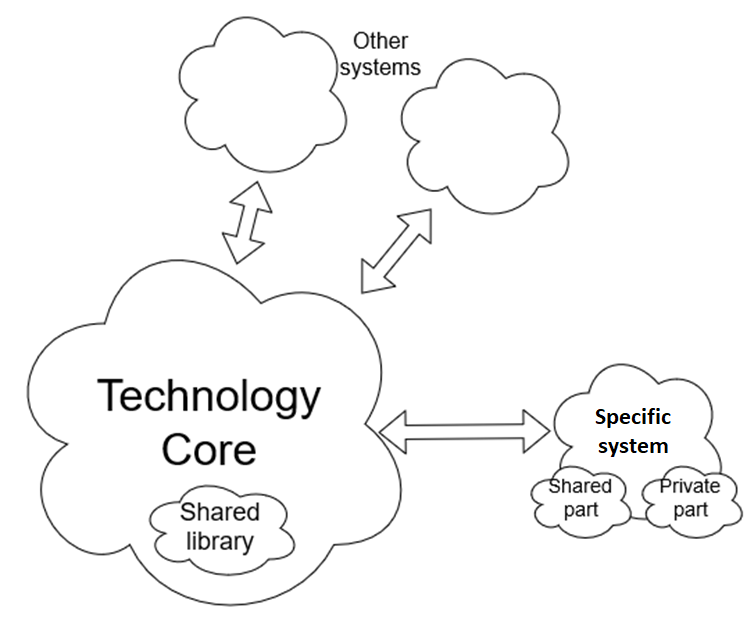
\includegraphics[width=0.6\textwidth]{figures/chapter0/ecosystem.png}}

\scnheader{Технология OSTIS}
\scnrelfromvector{текущие проекты}{Проект Экосистема OSTIS;Проект Метасистема IMS.ostis;Проект Семейство различных вариантов реализации универсального интерпретатора семантических моделей интеллектуальных систем\\
\scnaddlevel{1}
    \scnrelfromlist{подпроект}{Проект Программно реализованный на современных компьютерах универсальный интерпретатор семантических моделей интеллектуальных систем;Проект Семантический ассоциативный компьютер}
\scnaddlevel{-1}
;Проект Комплекс совместимых средств проектирования интеллектуальных систем\\
\scnaddlevel{1}
    \scnrelfromlist{подпроект}{Проект Встраиваемая типовая интеллектуальная система комплексной поддержки проектирования баз знаний;Проект Интеллектуальная система комплексной поддержки проектирования решателей задач интеллектуальных систем;Проект Интеллектуальная система комплексной поддержки проектирования вербальных интерфейсов интеллектуальных систем;Проект Интеллектуальная система комплексной поддержки проектирования невербальных интерфейсов}
\scnaddlevel{-1}
;Проект Семейство совместимых интеллектуальных справочных, обучающих и help-систем\\
\scnaddlevel{1}
    \scnrelfromlist{подпроект}{Проект Специализированные средства разработки совместимых интеллектуальных справочных, обучающих и help-систем различного назначения;Проект Комплекс семантически совместимых интеллектуальных справочных и обучающих систем по всем дисциплинам среднего образования;Проект Комплекс семантически совместимых интеллектуальных справочных и обучающих систем по всем дисциплинам, являющихся базовыми при подготовке инженеров по информационным специальностям;Проект Комплекс семантически совместимых интеллектуальных справочных и обучающих систем по всем специальным дисциплинам специальности ''Искусственный интеллект''{};Проект Семейство совместимых интеллектуальных справочных и обучающих систем по стандартам различного вида}
\scnaddlevel{-1}
;Проект Семейство совместимых интеллектуальных корпоративных систем ситуационного управления\\
\scnaddlevel{1}
    \scnrelfromlist{подпроект}{Проект Интеллектуальная корпоративная система ситуационного управления предприятием рецептурного производства;Проект Интеллектуальная корпоративная система ситуационного управления деятельностью выпускающей кафедры технического вуза}
\scnaddlevel{-1}
}
\scnrelfromvector{будущие проекты}{
Проект Семейство совместимых интеллектуальных систем автоматизации проектирования в различных областях;Проект Семейство совместимых порталов знаний\\
\scnaddlevel{1}
    \scnrelfrom{подпроект}{Проект Портал научных знаний по искусственному интеллекту}
\scnaddlevel{-1}
;Проект Семейство совместимых интеллектуальных систем экскурсионного обслуживания;Проект Семейство совместимых интеллектуальных геоинформационных систем;Проект Семейство совместимых интеллектуальных робототехнических систем и специализированных средств их разработки;Проект Семейство совместимых интеллектуальных систем персонального обслуживания и мониторинга\\
\scnaddlevel{1}
    \scnrelfromlist{подпроект}{Проект Интеллектуальная система персонального обслуживания и мониторинга пользователей и разработчиков компьютерных систем, входящих в Экосистему OSTIS;Проект Интеллектуальный персональный ассистент по взаимодействию с традиционными internet-системами и их пользователями;Проект Интеллектуальная система персонального комплексного медицинского мониторинга и контроля}
\scnaddlevel{-1}
}

\scnsegmentheader{Понятие технологии OSTIS}

\scnstartsubstruct

\scnheader{Технология OSTIS}
\scnidtf{Комплекс (семейство) технологий, обеспечивающих проектирование, производство, эксплуатацию и реинжиниринг интеллектуальных \textit{компьютерных систем (ostis-систем)}, предназначенных для автоматизации самых различных видов человеческой деятельности и в основе которых лежит смысловое представление и онтологическая систематизация знаний, а также агентно-ориентированная обработка знаний}
\scnidtf{Open Semantic Technology for Intelligent Systems}
\scnaddlevel{1}
\scntext{сокращение}{OSTIS}
\scnaddlevel{-1}
\scnidtf{Семейство (комплекс) \textit{ostis-технологий}}
\scnidtf{Комплексная открытая семантическая технология проектирования, производства, эксплуатации и реинжиниринга гибридных, семантически совместимых, активных и договороспособных \textit{интеллектуальных компьютерных систем}}
\scnheader{Технология OSTIS}
\scnrelfromset{принципы, лежащие в основе}{
\scnfileitem{Ориентация на разработку \textit{интеллектуальных компьютерных систем}, имеющих высокий уровень \textit{интеллекта} и, в частности, высокий уровень \textit{социализации}. Указанные системы, разработанные по \textit{Технологии OSTIS}, будем называть \textbf{ostis-системами}}
;\scnfileitem{Ориентация на \uline{комплексную} автоматизацию всех видов и областей \textit{человеческой деятельности} путем создания сети взаимодействующих и координирующих свою деятельность \textit{ostis-систем}. Указанную сеть \textit{ostis-систем} вместе с их пользователями будем называть \textbf{\textit{Экосистемой OSTIS}}}
;\scnfileitem{Поддержка перманентной эволюции \textit{ostis-систем} в ходе их эксплуатации.}
;\scnfileitem{\textit{Технология OSTIS} реализуется в виде сети \textit{ostis-систем}, которая является частью \textit{Экосистемы OSTIS}.
Ключевой \textit{ostis-системой} указанной сети является \textbf{Метасистема IMS.ostis} (Intelligent MetaSystem), реализующая \textbf{Ядро Технологии OSTIS}, которое включает в себя базовые (предметно независимые) методы и средства проектирования и производства \textit{ostis-систем} с интеграцией в их состав типовых встроенных подсистем поддержки эксплуатации и реинжиниринга \textit{ostis-систем}. Остальные \textit{ostis-системы}, входящие в состав рассматриваемой сети, реализуют различные специализированные \textit{ostis-технологии} проектирования различных классов \textit{ostis-систем}, обеспечивающих автоматизацию любых областей и \textit{видов человеческой деятельности}, кроме \textit{проектирования ostis-систем}.}
;\scnfileitem{Конвергенция и интеграция на основе смыслового представления знаний всевозможных научных направлений \textit{Искусственного интеллекта} (в частности, всевозможных базовых знаний и навыков решения интеллектуальных задач) в рамках \textit{Общей формальной семантической теории ostis-систем}.}
;\scnfileitem{Ориентация на разработку компьютеров нового поколения, обеспечивающих эффективную (в том числе, производительную) интерпретацию логико-семантических моделей \textit{ostis-систем}, представленных базами знаний этих систем и имеющих смысловое представление.}}

\scnsegmentheader{Понятие ostis-системы}

\scnstartsubstruct

\scnheader{ostis-система}
\scnidtf{\textit{интеллектуальная компьютерная система}, спроектированная и реализованная по требованиям и стандартам \textit{Технологии OSTIS}, которые задокументированы в \textit{Общей теории ostis-систем}}

\scnheader{ostis-система}
\scnidtf{интеллектуальная компьютерная система, построенная в соответствии с принципами и требованиями Технологии OSTIS}
\scnidtf{Множество ostis-систем различного назначения}
\scnaddlevel{1}
\scniselement{имя собственное}
\scnaddlevel{-1}
\scnidtf{Множество всевозможных интеллектуальных компьютерных систем, построенных по Технологии OSTIS}

\scnheader{ostis-система}
\scnsubset{интеллектуальная компьютерная система}
\scnidtf{\textit{интеллектуальная компьютерная система}, которая построена в соответствии с требованиями и стандартами \textit{Технологии OSTIS}, что обеспечивает существенное развитие целого ряда \textit{свойств} (способностей) этой \textit{компьютерной системы}, позволяющих значительно повысить \textit{уровень интеллекта} этой системы (и, прежде всего, ее \textit{уровень обучаемости} и \textit{уровень социализации})} 

\scnauthorcomment{Добавить классификацию из пояснения}

\scnsubdividing{индивидуальная ostis-система;коллективная ostis-система\\
\scnaddlevel{1}
    \scnsubdividing{простой коллектив ostis-систем;иерархический коллектив ostis-систем}   
\scnaddlevel{-1}
}

\scnheader{ostis-система}
\scnexplanation{интеллектуальная компьютерная система, разработанная, разрабатываемая или совершенствуемая по технологии OSTIS}
\scnnote{Когда речь идет о таком компоненте технологии OSTIS, как модели ostis-систем, фактически имеется в виду теория ostis-систем, включающая в себя строгое формальное уточнение того, как устроена ostis-система, какова ее архитектура, принципы организации памяти, принципы организации представления информации, принципы организации интерфейса с внешней средой (в том числе, с пользователями)}

\scnheader{ostis-система}
\scnrelfromset{принципы, лежащие в основе}{
\scnfileitem{Информация, хранимая в памяти \textit{ostis-системы}, имеет смысловое представление.}
;\scnfileitem{В основе организации решения задач в памяти \textit{ostis-системы} лежит \textit{агентно-ориентированная модель обработки информации}, управляемая ситуациями и событиями, возникающими в обрабатываемой информации (точнее, в обрабатываемой базе знаний).}
;\scnfileitem{Унификация базового набора (базовой системы) используемых понятий, что является основой обеспечения \textit{семантической совместимости} всех \textit{ostis-систем}.}
;\scnfileitem{В основе структуризации информации (базы знаний), хранимой в памяти \textit{ostis-системы}, лежит иерархическая система \textit{предметных областей} и соответствующих им \textit{формальных онтологий}.}
;\scnfileitem{Способность к пониманию (к семантическому погружению, к семантической интеграции) новых приобретаемых знаний (и, в том числе, новых навыков) в состав текущего состояния \textit{базы знаний}.}
;\scnfileitem{Способность к \textit{семантической конвергенции} (к обнаружению сходств) новых приобретаемых знаний (и, в частности, навыков) со знаниями, входящими в состав текущего состояния базы знаний \textit{ostis-системы}.}
;\scnfileitem{Способность \textit{ostis-системы} поддерживать высокий уровень своей \textit{семантической совместимости} (высокий уровень взаимопонимания) с другими \textit{ostis-системами}.}
;\scnfileitem{Способность ostis-системы согласовывать, координировать свою деятельность с другими \textit{ostis-системами}.}
;\scnfileitem{\scnauthorcomment{статья на OSTIS-2020}}
;\scnfileitem{\scnauthorcomment{статья на OSTIS-2020}}
;\scnfileitem{\scnauthorcomment{статья на OSTIS-2020}}
;\scnfileitem{\scnauthorcomment{статья на OSTIS-2020}}}
\scntext{следовательно}{Перечисленные свойства \textit{ostis-систем} свидетельствуют о том, что они имеют существенно более высокий \textit{уровень интеллекта} и, в частности, более высокий \textit{уровень социализации} по сравнению с современными \textit{интеллектуальными компьютерными системами}. \scnauthorcomment{См. начало Раздела 1.1}}

\scnheader{ostis-система}
\scnrelfromset{принципы, лежащие в основе}{
\scnfileitem{смысловое представление информации в памяти компьютерных систем, направленное на устранение недостатков современных компьютерных систем и технологий путем повышения уровня интеллектуальности компьютерных систем}
;\scnfileitem{децентрализация управления решателем задач
\begin{itemize}
	\item внутренняя МАС
	\item внешняя МАС
\end{itemize}}
;\scnfileitem{интеграция различных видов знаний}
;\scnfileitem{интеграция различных моделей решателей задач}
;\scnfileitem{ориентация на компьютеры нового поколения}
;\scnfileitem{обеспечение семантической совместимости компьютерных систем}
;\scnfileitem{обеспечение поддержания семантической совместимости компьютерных систем в ходе эволюции}
;\scnfileitem{способность к координации деятельности}}

\scnheader{ostis-система}
\scnrelfromset{принципы, лежащие в основе}{
\scnfileitem{Память ostis-системы является графодинамической (т.е. нелинейной (графовой) и структурно перестраиваемой). Переработка информации в памяти ostis-системы сводится не столько к изменению состояния элементов памяти (это происходит только при изменении синтаксического типа элементов и при изменении содержимого тех элементов, которые обозначают файлы), сколько к изменению \uline{конфигурации связей} между ними.}
;\scnfileitem{Хранение информации в памяти ostis-системы ориентируется на \uline{смысловое} представление информации – без синонимов, омонимов знаков и без семантической эквивалентности информационных конструкций.}
;\scnfileitem{С точки зрения архитектуры ostis-система представляет собой \uline{иерархическую} многоагентную систему с общедоступной памятью (т.е. с памятью, общедоступной \uline{всем} агентам ostis-системы). 
Заметим при этом, что общая память большинства исследуемых в настоящее время многоагентных систем является не общедоступной, а распределенной, т.е. представляет собой абстрактное (виртуальное) объединение, в состав которого входит память каждого агента многоагентной системы. Координация деятельности агентов ostis-системы при выполнении сложных \textit{действий в памяти} ostis-системы реализуется также через \textit{память ostis-системы} с помощью хранимых в памяти \textit{методов} решения различных классов задач, а также с помощью хранимых в памяти \textit{планов} решения конкретных задач.
На основании этого можно строить неограниченную иерархическую систему агентов ostis-системы – от элементарных агентов, обеспечивающих выполнение базовых действий в памяти ostis-системы, до неэлементарных агентов, представляющих собой коллективы (группы) элементарных и/или неэлементарных агентов, обеспечивающих решение различных типовых задач с помощью соответствующих методов и планов.}
;\scnfileitem{Организация выполнения \textit{ostis-системой действий во внешней среде} осуществляется следующим образом:
\begin{scnitemize}
	\item Выделяются классы \textit{элементарных действий во внешней среде}, для реализации каждого из которых вводятся \textit{эффекторные агенты} ostis-системы.
	\item Координация деятельности \textit{эффекторных агентов} ostis-системы при выполнении \textit{сложных действий во внешней среде} осуществляется через \textit{память ostis-системы} с помощью хранимых в памяти \textit{методов} и \textit{планов} решения различных задач во \textit{внешней среде}, а также с помощью \textit{рецепторных агентов} ostis-системы, обеспечивающих обратную связь и, соответственно, сенсомоторную координацию.
\end{scnitemize}}}

\scnheader{ostis-система}
\scnrelfromset{принципы, лежащие в основе}{
\scnfileitem{Способность понимать друг друга, а также любого своего пользователя
\scnaddlevel{-2}
\scnidtf {Совместимость используемых понятий (по терминам и по денотационной семантике)}
\scnidtf {Семантическая совместимость}
\scnaddlevel{2}}
;\scnfileitem{Способность поддерживать взаимопонимание в процессе индивидуальной эволюции, приводящей к расширению и/или корректировке системы используемых понятий}
;\scnfileitem{Способность координировать свою деятельность с другими системами при решении задач, которые усилиями одной (индивидуальной) интеллектуальной компьютерной системы не могут быть решены либо принципиально, либо за разумное время}}

\scnheader{ostis-система}
\scnrelfromset{принципы, лежащие в основе}{
\scnfileitem{Высокая степень индивидуальной обучаемости интеллектуальных компьютерных систем
\begin{itemize}
	\item гибкости
	\item стратифицированности
	\item рефлексивности
	\item универсальность средств представления и образования знаний
\end{itemize}}
;\scnfileitem{Высокая степень семантической совместимости и, как следствие, коллективной обучаемости интеллектуальных компьютерных систем
\begin{itemize}
	\item семантической совместимости
\end{itemize}}
;\scnfileitem{Основа для автоматизации рынка знаний}}

\scnmakeset{память*;ostis-система}
\scnrelfrom{сужение второго домена заданного отношения для заданного первого домена}{память ostis-системы}
\scnaddlevel{1}
\scnsubset{смысловая память}
\scnaddlevel{-1}


\scnmakeset{информация, хранимая в памяти кибернетической системы*;  ostis-система}
\scnrelfrom{сужение второго домена заданного отношения для заданного первого домена}{база знаний ostis-системы}
\scnaddlevel{1}
\scnsubset{смысловое представление информации}
\scnaddlevel{-1}


\scnheader{память ostis-системы}
\scnsubset{смысловая память}

\scnheader{информация, хранимая в памяти ostis-системы}
\scnsubset{смысловое представление информации}

\scnheader{решатель задач ostis-системы }
\scnsubset{агентно-ориентированная модель обработки информации в памяти}







































 

\scnendstruct

\end{SCn}


\scchapter[\scneditor{Шункевич Д.В.}]{Предметная область и онтология интеллектуальных компьютерных систем нового поколения}
\label{sem_mod_comp_sys}
\begin{SCn}

\scnsectionheader{\currentname}
\scnstartsubstruct

\scnrelfromlist{дочерний раздел}{\nameref{sd_sem_inf_rep}; \nameref{sd_agent_solvers};\nameref{sd_sem_ui}}
\scntext{аннотация}{Данный раздел и дочерние ему разделы являются уточнением и обоснованием наших предложений, направленных на построение компьютерных систем следующего поколения, основанных на смысловом представлении обрабатываемой информации.}
\scntext{основной тезис}{Для \uline{любой} \textit{компьютерной системы} можно построить эквивалентную ей логико-семантическую модель, основанную на смысловом представлении обрабатываемой информации}


\scnheader{Предметная область логико-семантических моделей компьютерных систем, основанных на смысловом представлении информации}
\scniselement{предметная область}
\scnsdmainclasssingle{логико-семантическая модель компьютерной системы}
\scnsdclass{семантическая совместимость компьютерных систем;компьютерная система, основанная на смысловом представлении информации}


\scnheader{логико-семантическая модель компьютерной системы}
\scnexplanation{Главным фактором обеспечения совместимости различных видов знаний, различных моделей решения задач и различных компьютерных систем в целом является 
\begin{scnitemize}
    \item унификация (стандартизация) представления информации в памяти компьютерных систем;
    \item унификация принципов организации обработки информации в памяти компьютерных систем.
\end{scnitemize}

Унификация представления информации, используемой в компьютерных системах, предполагает:
\begin{scnitemize}
    \item синтаксическую унификацию используемой информации – унификацию формы представления (кодирования) этой информации. При этом следует отличать:
    \begin{scnitemizeii}
    	\item кодирование информации в памяти компьютерной системы (внутреннее представление информации);
    	\item внешнее представление информации, обеспечивающее однозначность интерпретации (понимания, трактовки) этой информации разными пользователями и разными компьютерными системами;
    \end{scnitemizeii}
    \item семантическую унификацию используемой информации, в основе которой лежит согласование и точная спецификация всех (!) используемых понятий (концептов) с помощью иерархической системы формальных онтологий.
\end{scnitemize}}

\scnresetlevel
\scnheader{стандарт}
\scnhaselement{Стандарт OSTIS}
\scnaddlevel{1}
\scnidtf{Предлагаемый нами стандарт логико-семантических моделей компьютерных систем,  основанных на смысловом представлении информации, и технологии разработки таких моделей и соответствующих компьютерных систем}
\scnaddlevel{-1}
\scnidtf{знания о структуре и принципах функционирования искусственных систем соответствующего класса}
\scnidtf{онтология искусственных систем некоторого класса}
\scnidtf{теория искусственных систем некоторого класса}
\scnexplanation{Важно отметить, что грамотная унификация (стандартизация) должна не ограничивать творческую свободу разработчика, а гарантировать \uline{совместимость} его результатов с результатами других разработчиков. Подчеркнем также, что текущая версия любого \textit{стандарта} -- это не догма, а только опора для дальнейшего его совершенствования.

Целью качественного \textit{стандарта} является не только обеспечения совместимости технических решений, но и минимизация дублирования (повторения) таких решений. Один из важных критериев качества \textit{стандарта} -- ничего лишнего.

\textit{Стандарты}, как и другие важные для человечества \textit{знания}, должны быть формализованы и должны постоянно совершенствоваться с помощью специальных \textit{интеллектуальных компьютерных систем}, поддерживающих процесс эволюции стандартов путем согласования различных точек зрения.}
\scnaddlevel{-1}

\scnheader{семантическая совместимость компьютерных систем}
\scnexplanation{Уровень совместимости \textit{компьютерных систем} определяется трудоемкостью реализации процедур интеграции (объединения, соединения знаний этих систем), а также трудоемкостью и глубиной интеграции входящих в эти системы \textit{решателей задач} (интеграции навыков и интерпретаторов этих навыков). Подчеркнем при этом, что интеграция интеграции рознь -- от эклектики до гибридности и синергетичности дистанция огромного размера.
	
	Совместимые \textit{компьютерные системы} -- это компьютерные системы, для которых существует автоматически выполняемая процедура их интеграции, превращающая эти системы в единую \textit{гибридную систему}, в рамках которой каждая интегрируемая компьютерная система в процессе своего функционирования может свободно использовать любые необходимые информационные ресурсы (знания и навыки), входящие в состав другой интегрируемой компьютерной системы.
	
	Целостную \textit{компьютерную систему} можно рассматривать как решатель задач, интегрировавший несколько моделей решения задач и обладающий средствами взаимодействия с внешней для себя средой (с другими компьютерными системами, с пользователями).
	
	Таким образом, для того, чтобы повысить уровень совместимости \textit{компьютерных систем}, необходимо преобразовать их к виду \textit{многоагентных систем}, работающих над общей семантической памятью. Такие \textit{компьютерные системы} не всегда целесообразно непосредственно объединять (интегрировать) в более крупные \textit{компьютерные системы}. Иногда целесообразнее их объединять в \textit{коллективы взаимодействующих компьютерных систем}. Но при создании таких коллективов компьютерных систем унификация и совместимость таких систем также очень важны, т.к. существенно упрощают обеспечение высокого уровня их взаимопонимания. Так, например, противоречия между компьютерными системами, входящими в коллектив, можно обнаруживать путем анализа на непротиворечивость \textit{виртуальной объединенной базы знаний} этого коллектива. Более того, непротиворечивость указанной виртуальной базы знаний можно считать одним из критериев семантической совместимости систем, входящих в соответствующий коллектив.}

\scnheader{компьютерная система, основанная на смысловом представлении информации}
\scnexplanation{Предлагаемое нами устранение проблем современных информационных технологий путем перехода к \textit{смысловому представлению информации} в памяти компьютерных систем фактически преобразует современные компьютерные системы (в том числе и современные интеллектуальные компьютерные системы) в \textit{компьютерные системы, основанные на смысловом представлении информации}, которые являются не альтернативной ветвью развития \textit{компьютерных систем}, а естественным этапом их эволюции, направленным на обеспечение высокого уровня их \textit{обучаемости} и, в первую очередь, \textit{совместимости}.
	
	Архитектура \textit{компьютерных систем, основанных на смысловом представлении информации} (см. \textit{Рис. Архитектура компьютерных систем, основанных на смысловом представлении информации}) практически совпадает с архитектурой \textit{интеллектуальных компьютерных систем}, основанных на знаниях. Отличие здесь заключаются в том, что в \textit{компьютерных системах, основанных на смысловом представлении информации}:
	\begin{scnitemize}
		\item база знаний имеет смысловое представление;
		\item интерпретатор знаний и навыков представляет собой коллектив \textit{агентов}, осуществляющих обработку \textit{базы знаний}.
	\end{scnitemize}
	
	Как следствие этого, \textit{компьютерные системы, основанная на смысловом представлении информации}, обладают высоким уровнем \textit{обучаемости}, т.е. способностью быстро приобретать новые и совершенствовать уже приобретенные знания и навыки и при этом не иметь никаких ограничений на вид приобретаемых и совершенствуемых ею знаний и навыков, а также на их совместное использование.
	
	Более того, при согласовании соответствующих стандартов, а также при перманентном совершенствовании этих стандартов и при грамотной их поддержке в условиях интенсивной эволюции как самих стандартов, так и \textit{компьютерных систем, основанных на смысловом представлении информации} (речь идет о постоянной поддержке соответствия между текущим состоянием компьютерных систем и текущим состоянием эволюционируемых стандартов), \textit{компьютерные системы, основанные на смысловом представлении информации} и их компоненты обладают весьма высокой степенью \textit{совместимости}.
	
	Это, в свою очередь, практически исключает дублирование инженерных решений и дает возможность существенно ускорить разработку \textit{компьютерных систем, основанных на смысловом представлении информации} с помощью постоянно расширяемой библиотеки многократно используемых и совместимых между собой компонентов. 
	
	Основным лейтмотивом перехода от современных компьютерных систем (в том числе интеллектуальных) к \textit{компьютерным системам, основанным на смысловом представлении информации}, хранимой в ее памяти, является создание \textbf{\textit{общей семантической теории компьютерных систем}}, включающей в себя:
	\begin{scnitemize}
		\item cемантическую теорию \textit{знаний} и \textit{баз знаний};
		\item семантическую теорию \textit{задач} и \textit{моделей решения задач};
		\item cемантическую теорию \textit{взаимодействия информационных процессов};
		\item cемантическую теорию пользовательских и, в том числе, естественно-языковых интерфейсов;
		\item cемантическую теорию невербальных (сенсорно-эффекторных) интерфейсов;
		\item теорию универсальных интерпретаторов \textit{логико-семантических моделей компьютерных систем} и, в частности, теорию семантических компьютеров.
	\end{scnitemize}
	
	Эпицентром следующего этапа развития информационных технологий является решение проблемы обеспечения \textbf{\textit{семантической совместимости}} \textit{компьютерных систем} и их компонентов. Для решения этой проблемы необходим
	\begin{scnitemize}
		\item переход от традиционных компьютерных систем и от современных интеллектуальных компьютерных систем к \textit{компьютерным системам, основанным на смысловом представлении информации};
		\item разработка \textit{стандарта компьютерных систем, основанных на смысловом представлении информации}.
	\end{scnitemize}    
	
	Очевидно, что \textit{компьютерные системы, основанных на смысловом представлении информации} являются компьютерными системами нового поколения, устраняющие многие недостатки современных компьютерных систем. Но для массовой разработки таких систем необходима соответствующая технология, которая должна включать в себя  
	
	\begin{scnitemize}        
		\item теорию \textit{компьютерных систем, основанных на смысловом представлении информации} и комплекс всех стандартов, обеспечивающих совместимость разрабатываемых систем;
		\item методы и средства проектирования \textit{компьютерных систем, основанных на смысловом представлении информации};
		\item методы и средства перманентного совершенствования самой технологии.
	\end{scnitemize}
}

\scnheader{Рис. Архитектура компьютерных систем, \textit{основанных на смысловом представлении информации}}
\scneqfile{\\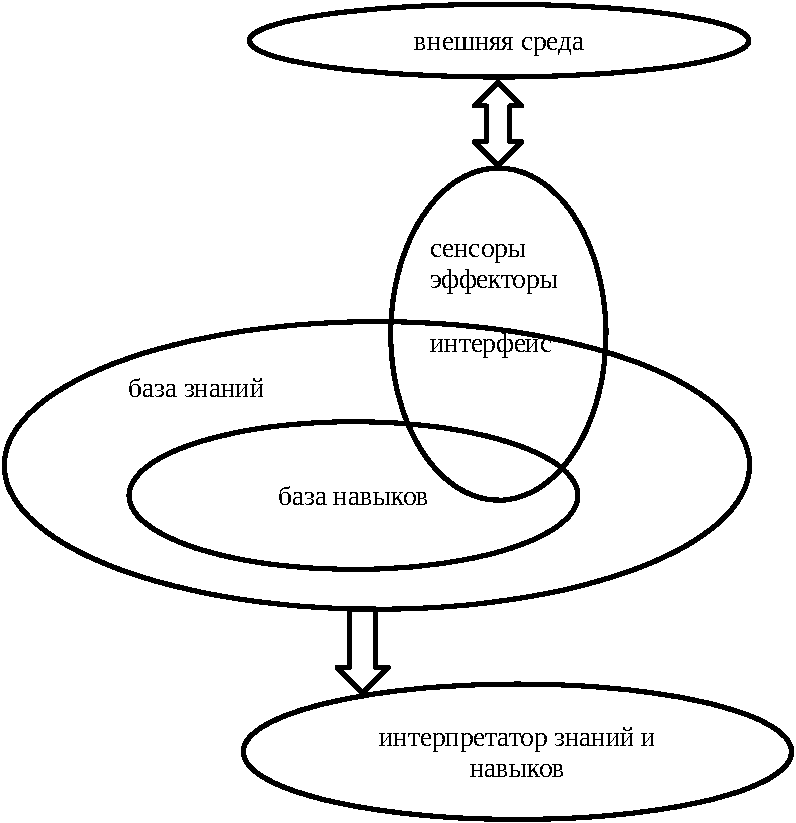
\includegraphics[width=0.5\linewidth]{figures/arch.pdf}\\}

\bigskip
\scnendstruct \scnendcurrentsectioncomment

\end{SCn}

\scsection[\scneditor{Банцевич К.А.}]{Предметная область и онтология смыслового представления информации}
\label{sd_sem_inf_rep}
\begin{SCn}

\scnsectionheader{\currentname}

\scnstartsubstruct

\scnrelto{частная предметная область и онтология}{Предметная область и онтология информационных конструкций}

\scnsdmainclasssingle{смысловое представление информации}

\scnsdclass{семантическая сеть\\
	\scnaddlevel{1}
	\scnsubdividing{нерафинированная семантическая сеть;рафинированная семантическая сеть}
	\scnsubdividing{абстрактная семантическая сеть\\
		\scnaddlevel{1}
		\scnidtf{семантическая сеть, абстрагирующаяся от того, как физически представлены ее элементарные (атомарные) фрагменты, а также связи инцидентности между этими фрагментами}
		\scnaddlevel{-1}
	;графически представленная семантическая сеть\\
		\scnaddlevel{1}
		\scnidtf{нарисованная семантическая сеть}
		\scnaddlevel{-1}
	;семантическая сеть, хранимая в графодинамической памяти\\
		\scnaddlevel{1}
		\scnrelboth{следует отличать}{представление семантической сети в адресной памяти}
			\scnaddlevel{1}
			\scnnotsubset{семантическая сеть}
			\scnidtf{представление семантической сети в виде линейной информационной конструкции, которая хранится в адресной памяти и которая, строго говоря, уже не является семантической сетью, но является информационной конструкцией, семантически эквивалентной соответствующей (представляемой) семантической сети}			
			\scnaddlevel{-1}
		\scnaddlevel{-1}}
	\scnaddlevel{-1}
;язык семантических сетей\\
	\scnaddlevel{1}
	\scnidtf{язык, все тексты которого являются семантическими сетями}
	\scnsubdividing{специализированный язык семантических сетей;универсальный язык семантических сетей}
	\scnsuperset{язык рафинированных семантических сетей}
	\scnaddlevel{-1}}

\scnrelfromvector{рассматриваемые вопросы}{
\scnfileitem{Что такое семантические сети и в чем их принципиальное отличие от других вариантов представления информации}
;\scnfileitem{До какой степени можно минимизировать алфавит элементов семантических сетей}
;\scnfileitem{Можно ли все описываемые связи свести к бинарным связям и почему это целесообразно}
;\scnfileitem{Можно ли разработать \uline{универсальный} язык семантических сетей}
;\scnfileitem{До какой степени можно упростить синтаксические структуры семантических сетей до, условно говоря, рафинированного вида}
;\scnfileitem{Какими достоинствами обладает семантические сети}}

\scnrelfromlist{ссылка}{Понятие Технологии OSTIS\\
	\scnaddlevel{1}
	\scntext{аннотация}{В указанном сегменте \textit{Стандарта OSTIS} рассматриваются принципы, лежащие в основе \textit{Технологии OSTIS}, основным из которых является ориентация на использование \textit{\uline{универсального} языка рафинированных семантических сетей} в качестве внутреннего языка \textit{интеллектуальных компьютерных систем}}
	\scnaddlevel{-1}
;Описание внутреннего языка ostis-систем\\
	\scnaddlevel{1}
	\scntext{аннотация}{В указанном разделе \textit{Стандарта OSTIS} рассматриваются принципы, лежащие в основе \textit{универсального языка рафинированных семантических сетей}, используемого в качестве внутреннего языка \textit{ostis-систем} -- \textit{интеллектуальных компьютерных систем} следующего поколения}
	\scnaddlevel{-1}
;Описание языка графического представления знаний ostis-систем\\
	\scnaddlevel{1}
	\scntext{аннотация}{В указанном разделе \textit{Стандарта OSTIS} рассматриваются принципы, лежащие в основе универсального языка графически представленных семантических сетей, используемого в \textit{пользовательском интерфейсе ostis-систем}}
	\scnaddlevel{-1}
;\scncite{Birukov1960};\scncite{Morris2001};\scncite{Pirs2009};\scncite{Stepanov1971};\scncite{MelchukST}}
	

\bigskip
\scnfragmentcaption

\scnheader{знак}
\scnidtf{фрагмент информационной конструкции, обладающий свойством, \uline{обозначать} некоторую сущность (объект), которая наряду с другими сущностями описывается указанной информационной конструкцией}
\scnnote{\uline{Форма} представления знаков в известной степени условна и является результатом соглашения между носителями соответствующего языка. Знак может быть, например, представлен:
	\begin{scnitemize}
	\item  в виде фрагмента речевого сообщения (последовательностью фонем);
	\item в виде строки символов (последовательности букв) в заданном алфавите;
	\item в виде иероглифа, пиктограммы;
	\item в виде жеста.
	\end{scnitemize}}
\scniselementrole{ключевой знак}{Предметная область и онтология информационных конструкций}
	\scnaddlevel{1}
	\scnhaselement{раздел Базы знаний IMS.ostis}
	\scnaddlevel{-1}
\scntext{характеристика элементов данного множества}{Знаки, используемые в различных языках, характеризуются:
	\begin{scnitemize}
	\item синтаксической структурой, по совпадению (изоморфизму) которых для разных знаокв предполагается их синонимия;
	\item денотационной семантикой, т.е. той сущностью, которая обозначается соответствующим знаком;
	\item типом (классом) обозначаемой сущности, которая может быть:
	 	\begin{scnitemizeii}
		\item материальным(физическим) элементом (точкой) абстрактного пространства, множеством, которое может быть:
			\begin{scnitemizeiii}
			\item связью;
			\item классом;
			\item структурой;
			\end{scnitemizeiii}
		\item реальной и вымышленной сущностью;
		\item константной (конкретной) и переменной (произвольной) сущностью;
		\item постоянно существующей и временно существующей сущностью (прошлой, настоящей, будущей);		
		\end{scnitemizeii}
	\item множеством тех связей, которые связывают сущность, обозначаемую данным знаком с другими сущностями, а также, если данный знак обозначает некоторую связь, множеством сущностей, которые связаны этой связью, т.е. сущностей, являющихся компонентом этой связи;
	\item текущим статусом самого знака в памяти кибернетической системы, который может быть:
		\begin{scnitemizeii}
			\item логически удаленным знаком;
			\item настоящим знаком;
			\item предлагаемым (возможно, будущим) знаком.
		\end{scnitemizeii}
	\end{scnitemize}}
	
\scnheader{денотат*}
\scnidtf{денотат заданного знака*}
\scnidtf{объект, обозначаемый заданным знаком*}
\scnidtf{денотационная семантика заданного знака*}
\scnidtf{смысл заданного знака*}
\scnidtf{Бинарное ориентированное отношение, каждая пара которого связывает:
	\begin{scnitemize}
			\item некоторый знак, представленный в той или иной форме в тексте исследуемого языка;
			\item \uline{со знаком} той сущности, которая обозначается указанным выше знаком в рамках используемого метаязыка.
		\end{scnitemize}}
\scnnote{Данное отношение используется, когда с помощью одного языка необходимо описать денотационную семантику другого языка. Фактически речь идет о переводе заданного знака, входящего в состав некоторого рассматриваемого текста, принадлежащего некоторому исследуемому языку (языку-объекту), на некоторый метаязык (в нашем случае на SC-код), денотационная семантика которого нам считается априори известной. Указанный перевод есть связь заданного знака с синонимичным ему знаком, входящим в состав текста, принадлежащего указанному метаязыку.}
\scnrelboth{обратное отношение}{внешний sc-идентификатор*}
\scnaddlevel{1}
\scnidtf{быть знаком, обозначающим заданную сущность*}
\scnaddlevel{-1}
\scniselementlist{ключевой знак}{Описание внешних идентификаторов знаков, входящих в тексты внутреннего языка ostis-систем\\
	\scnaddlevel{1}
	\scniselement{раздел Базы знаний IMS.ostis}
	\scnaddlevel{-1}
;Предметная область и онтология знаков, входящих в тексты внутреннего языка ostis-систем\\
	\scnaddlevel{1}
	\scniselement{раздел Базы знаний IMS.ostis}
	\scnaddlevel{-1}}
	
\scnheader{информационная конструкция}
\scnidtf{информация}
\scnnote{В общем случае информационная конструкция представляет собой сложную иерархическую структуру, каждому уровню иерархии которой соответствует определенный класс информационных конструкций.}
\scnsuperset{синтаксически элементарный фрагмент информационной конструкции}
	\scnaddlevel{1}
	\scnidtf{атомарный фрагмент информационной конструкции}
	\scnidtf{элемент информационной конструкции}
	\scnnote{Примерами таких элементарных фрагментов информационных конструкций являются буквы}
	\scnsuperset{буква}
	\scnaddlevel{-1}
\scnsuperset{простой знак}
	\scnaddlevel{1}
	\scnidtf{семантически элементарный фрагмент информационной конструкции}
	\scnsubset{знак}
	\scnaddlevel{-1}
\scnsuperset{выражение}
\scnaddlevel{1}
	\scnidtf{сложный (непростой) знак}
	\scnidtf{знак, являющийся одновременно некоторым знанием обозначаемой сущности (спецификацией этой сущности)}
	\scnidtf{знак, построенный как выражение вида "тот, который..."{}}
	\scnidtf{знак, в состав которого входят другие знаки}
	\scnsubset{знак}
	\scnaddlevel{-1}
\scnsuperset{простой текст}
	\scnaddlevel{1}
	\scnidtf{минимальная синтаксически целостная и корректная (правильная) информационная конструкция, включающая в себя:
	\begin{scnitemize}
	\item знак некоторой описываемой связи;
	\item минимальную спецификацию указанного знака связи (указание отношения, которому это связь принадлежит);
	\item указание \uline{всех} компонентов описываемой связи (знаков всех сущностей, связываемых этой связью, и/или всех знаков, связываемых этой связью -- описываемая связь может связывать не только "внешние"{} описываемые сущности, но и сами знаки);
	\item если описываемая связь не является бинарной, то связи с её компонентами могут потребовать явного представления знаков этих связей с дополнительным указанием роли этих компонентов.
	\end{scnitemize}}
	\scnsubset{текст}
	\scnaddlevel{-1}
\scnsuperset{сложный текст}
	\scnaddlevel{1}
	\scnidtf{информационная конструкция, являющаяся результатом соединения нескольких простых текстов}
	\scnsubset{текст}
	\scnaddlevel{-1}
\scnsuperset{простое знание}
	\scnaddlevel{1}
	\scnidtf{минимальная семантические целостная информационная конструкция}
	\scnidtf{знание, в состав которого не входят другие знания}
	\scnsubset{знание}
	\scnaddlevel{-1}	
\scnsuperset{сложное знание}
	\scnaddlevel{1}
	\scnidtf{информационная конструкция, являющаяся результатом соединения нескольких простых знаний}
	\scnidtf{знание, в состав которого не входят другие знания}
	\scnsubset{знание}
	\scnaddlevel{-1}	
\scniselementrole{ключевой знак}{Предметная область и онтология информационных конструкций}
\scnaddlevel{1}
	
\scnaddlevel{-1}

\bigskip
\scnfragmentcaption

\scnheader{смысловое представление информации}
\scnidtf{смысловая форма представления информации}
\scnidtf{смысловое представление информационной конструкции}
\scnidtf{знаковая конструкция (текст), представленная в смысловой форме}
\scnidtf{смысловое представление информационной конструкции}
\scnidtftext{часто используемый sc-идентификатор}{смысл}
\scnidtf{смысловое представление}
\scnidtf{семантическое представление информации}

\scntext{основной принцип}{Как можно меньше лишнего, не имеющего отношения к смыслу представляемой информации.}
\scnidtf{такое представление информационной конструкции, которое существенно прощает соответствие между структурой самой этой информационной конструкции и описываемой (отображаемой) ею конфигурацией связей между рассматриваемыми (исследуемыми) сущностями}
\scnidtf{смысловое представление знаковой конструкции}
\scnidtf{абстрактная знаковая конструкция, являющаяся \uline{инвариантом} соответствующего максимального класса семантически эквивалентных знаковых конструкций}
\scnidtf{смысл информационной конструкции}
\scnidtf{денотационная семантика информационной конструкции}
\scnidtf{смысловое представление информационной конструкции}


\scnnote{Суть (смысл, денотационная семантика) любой информационной конструкции (информационной модели) сводится к описанию системы (конфигурации) связей между списываемыми (рассматриваемыми) сущностями. Важно, чтобы эта суть не была \uline{закамуфлирована} различными "синтаксическими"{} деталями, не имеющими никакого отношения к указанному смыслу (синтаксическая структура знаков, многократное повторение одного и того же знака, синонимия, омонимия, местоимения, предлоги, знаки препинания, разделители, ограничители, падежи и т.п.) а обусловленными \uline{формой} представления информационных конструкций, например, их линейностью.}


\scnexplanation{Смысловое представление любой информации в конечном счете сводится:
	\scnaddlevel{1}
	\begin{scnitemize}
		\item{к перечню знаков конкретных описываемых сущностей - как первичных сущностей, так и вторичных сущностей, которые сами являются информационными конструкциями (фрагментами данной конструкции)};
		\item{к явному описанию связи между знаками вторичных сущностей и самими этими сущностями (т.е. фрагментами информационной конструкции)};
		\item{к описанию других связей между описываемыми сущностями}
	\end{scnitemize}
}
\scnaddlevel{-1}

\scnexplanation{Формализация смысла представляемой информации, т.е. строгое уточнение того, что такое \textit{смысловое представление информации}, является объективной основой для \uline{унификации} представления информации в \textit{памяти компьютерных систем} и \uline{ключом} к решению многих проблем семантической совместимости и эволюции компьютерных систем и технологий.

Согласно \textit{Мартынову В. В.} (\scncite{Martynov}), <<фактически всякая мыслительная деятельность человека (не только научная), как полагают многие ученые, использует \uline{внутренний семантический код}, на который переводят с естественного языка и с которого переводят на естественный язык. Поразительная способность человека к идентификации огромного множества структурно различных фраз с одинаковым \textit{смыслом} и способность \uline{запомнить смысл вне этих фраз} убеждает нас в этом.>>

Приведем также слова \textit{Мельчука И. А.} (\scncite{MelchukST}):

<<Идея была следующая -- язык надо описывать следующим образом: надо уметь записывать смыслы фраз. \uline{Не фразы, а их \textit{смыслы}}, что отдельно. Плюс построить систему, которая по смыслу строит фразу. Это та область или тот поворот исследований, при котором интуиция способного лингвиста работает лучше всего: как выразить на данном языке данный смысл. Это -- то, для чего лингвистов учат..

Лингвистический \textit{смысл} научного текста -- это совсем не то, что ты, читая его, из него извлекаешь. Это, очень грубо говоря, инвариант синонимических перифраз. Ты можешь один и тот же смысл выразить очень многими способами. Когда ты говоришь, то можешь сказать по-разному: ``Сейчас я налью тебе вина'', или: ``Дай, я тебе предложу вина'', или: ``Не выпить ли нам по бокалу?'', -- все это имеет один и тот же смысл. И вот можно придумать, как записывать этот \textit{смысл}. Именно его. Не фразу, а \textit{смысл}. И работать надо от этого \textit{смысла} к реальным фразам. Синтаксис там по дороге тоже нужен, но он нужен именно по дороге, он не может быть ни конечной целью, ни начальной точкой. Это -- промежуточное дело.>> (\scncite{Melchuk}).
}

\scnnote{Грамотная унификация (стандартизация) \textit{смыслового представления информации} не должна привести к ограничению творческой свободы авторов различного вида публикуемых научно-технических знаний (и, в том числе, разработчиков \textit{баз знаний}), не должна гарантировать \textit{семантическую совместимость} различных \textit{знаний}, представленных различными авторами (разумеется, при условии соблюдения соответствующих правил построения этих \textit{знаний}). При этом любые \textit{стандарты} (в том числе и принятые стандарты \textit{смыслового представления информации}) должны постоянно эволюционировать. Текущая версия любого стандарта должна быть не догмой, а точкой опоры для дальнейшего совершенствования этого стандарта.}

\scnsuperset{УСК}
\scnaddlevel{1}
\scnidtf{Универсальный Семантический Код}
\scnrelfrom{автор}{Мартынов В. В.}
\scnnote{Разработанный Мартыновым В. В. Универсальный Семантический Код стал важнейшим этапом создания универсальных формальных средств смыслового представления знаний. Основная методологическая идея \textit{Мартынова В. В.}, касающаяся построения \textit{языка смыслового представления знаний}, заключается в том, чтобы выделить смысловые "кирпичики"{}, имеющие достаточно общий характер, а многообразие конкретных смыслов конструировать комбинаторно за счёт различных комбинаций (конфигураций) из этих "кирпичей"{}. Это можно назвать принципом минимизации типов атомарных смысловых фрагментов.}
\scnrelto{ключевой знак}{\scncite{Martynov1984}}


\scnheader{смысловое представление информации*}
\scnidtfexp{\textit{Бинарное ориентированное отношение}, каждая \textit{пара} которого связывает некоторую \textit{информационную конструкцию} со смысловым представлением этой \textit{информационной конструкции*}.}

\scnsubset{формализация*}

\bigskip
\scnfragmentcaption

\scnheader{формализация*}
\scniselement{бинарное ориентированное отношение}
\scnidtf{формализация информации*}
\scnidtf{пара, связывающая менее формализованное и более формализованное представление некоторой информации*}
\scnidtf{формализация информационной модели некоторой описываемой (моделируемой) системы взаимосвязанных сущностей*}
\scnidtf{Бинарное ориентированное отношение, каждая \textit{пара} которого, связывает два \textit{семантически эквивалентных} знания, второе из которых является более точным (более точно сформированным) знанием по сравнению с первым \textit{знанием}*.}
\scnexplanation{Повышение точности (строгости) формулировки знания -- минимизация (а в идеале -- исключение) \uline{неоднозначной} семантической интерпретации этой формулировки, т.е. несоответствия того, что хотел "сказать"{} автор формулировки, и того, как его поняли. Формализация знаний предполагает (1) точное (строгое) описание \textit{синтаксиса и денотационной семантики} того \textit{языка}, на котором формулируются \textit{знания} и (2) максимально возможное \uline{упрощение} синтаксических и семантических принципов, лежащих в основе указанного \textit{языка}. Очевидно, что \textit{естественные языки} указанным требованиям не удовлетворяют и, следовательно, не могут быть основой для точной формулировки \textit{научно-технических знаний} и, соответственно, для представления этих \textit{знаний} в \textit{памяти интеллектуальных компьютерных систем}. Очевидно также, что разработка \textit{\uline{универсального} языка} формального представления научно-технических знаний является \uline{основой} для глубокой конвергенции различных научно-технических дисциплин, для расширения областей применения современной математики и даже для появления новых разделов математики, которые, например, изучают общие свойства \textit{универсального смыслового пространства} и, в частности, свойство семантического расстояния(семантической близости) как между различными \textit{знаками}, так и между различными \textit{знаковыми конструкциями} (конфигурациями знаков).}
\scnaddlevel{1}
\scnnote{Слово "математика"{} означает "точное знание"{}.}
\scnaddlevel{1}
\scnrelto{цитата}{\scncite{Arnold2012}}
\scnaddlevel{-2}

\scnnote{Формализация информационной модели есть не что иное как "движение"{} в сторону семантического (смыслового) представления этой модель, т.е. переход к такому представлению этой модели, в котором мы избавляемся от всего, не имеющего отношения к сути моделируемой системы и касающегося только способа построения этой модели (т.е. её синтаксической структуры). }
\scnnote{Нет проблемы записать любое \textit{знание} в компьютерную \textit{память}. Для этого надо придумать соответствующий формат их кодирования. Но есть проблема представить это \textit{знание} так, чтобы с ним было легко работать, чтобы с использованием этого \textit{знания} можно было достаточно удобно (без лишних накладных расходов, обусловленных выбранным способом представления) решать самые различные информационные \textit{задачи} (задачи интеграции знаний, информационного поиска по базе знаний, верификации и оптимизации баз знаний, логического вывода, поиска способов решения задач, хранимых в базе знаний и т. д.).
Какими характеристиками должно обладать удобное представление знаний, удовлетворяющее указанным требованиям. Очевидно, что такое представление есть не что иное, как формальная (математическая) модель, семантически эквивалентная этим знаниям. Т.е. удобно представить знание -- это фактически построить соответствующую этому знанию \textit{математическую модель}.
Для интеллектуальных компьютерных систем важно не просто приобрести знания, но и представить их в такой форме, которая была бы удобна не только для человека (пользователя и разработчика), но и для различных компьютерных систем, т.е. не требовала бы переоформление (перезаписи) этих знаний для различных компьютерных систем. Очевидно, что такая форма записи (представления) знаний должна быть абсолютно не зависящий от различных компьютерных платформ.
Это и есть главная цель формализации знаний, обеспечивающей эффективную автоматизацию обработки этих знаний.}
\scnheader{формальное представление информации}\\
\scnsubset{информация}
\scnaddlevel{1}
\scnidtf{информационная конструкция}
\scnaddlevel{-1}
\scntext{вопрос}{Почему разработка и использование формальных моделей (математических моделей) представления \textit{информации} является важнейшим этапом развития любой научной и научно-технической дисциплины.
}\scnaddlevel{1}
\scnrelfromset{ответ}{\scnfileitem{Формализация любой \textit{предметной области} даёт возможность более конструктивно накапливать, интегрировать, понимать и систематизировать новые \textit{знания} об этой \textit{предметной области}};
\scnfileitem{Формализация \textit{предметной области} обеспечивает более строгую верификацию, обоснование (аргументацию, доказательство) и согласование различных точек зрения};
\scnfileitem{Формализация \textit{предметной области} создает условия для разработки строгих и легко воспроизводимых (реализуемых) \textit{методов} решения различных \textit{классов задач}}}
\scnaddlevel{1}
\scnrelto{достоинства}{формальное представление информации}
\scnaddlevel{-2}
\scnidtf{формальное (формализованное) представление информационной конструкции}
\scnsubset{смысловое представления информации}
\scnnote{Высшим уровнем качества \textit{формального представления информации} является смысловое представление этой информации}
\scnidtf{формальная модель системы описываемых взаимосвязанных сущностей}
\scnidtf{математическая модель системы описываемых взаимосвязанных сущностей}
\scnidtf{формула}
\scnnote{Сам термин ``\textit{формальное представление информации}'' свидетельствует о том, что при таком представлении \textit{информации} сама \uline{форма} представляемой информационной конструкции (т.е. синтаксическая структура этой конструкции) имеет очевидную аналогию с описываемой конфигурацией связей между соответствующими соответствующими описываемыми \textit{сущностями}.
В предельном "идеальном"{} случае указанная аналогия между формой и смыслом информационной конструкции должна быть изоморфизмом.}
\scnnote{Формализация формализации рознь и, соответственно, степень приближения формы представления информации к "идеальному"{} смысловому представлению может быть различной. Разработка такого "идеального"{} \textit{языка смыслового представления информации} должна руководствоваться следующими основными критериями:
	\begin{scnitemize}		
		\item максимально возможное упрощения синтаксиса (как можно меньше синтаксических излишеств и синтаксического разнообразия).
		\item обеспечение \uline{универсальности} языка.
	\end{scnitemize}

Подчеркнем, что обеспечение универсальности \textit{языка смыслового представления информации} является весьма нетривиальной задачей, т.к. сложно одновременно достигнуть две противоречащие друг другу цели- обеспечить простоту синтаксиса языка и его неограниченную семантическую мощность. Косвенным подтверждением этого является большое количество созданных человечеством специализированных \textit{формальных языков}, \textit{языков смыслового представления информации} и даже \textit{языков семантических сетей}, что свидетельствует о востребованности \textit{смыслового представления информации}.}
\scnsubdividing{формальное представление информации, не являющееся смысловым
;смысловое представление информации, не являющееся семантической сетью
;нерафинированная семантическая сеть
\scnaddlevel{1}
\scnidtf{смысловое представления информации 2-го уровня}
\scnaddlevel{-1}
;рафинированная семантическая сеть
\scnaddlevel{1}
\scnidtf{смысловое представление информации 3-го уровня}
\scnaddlevel{-1}}

\bigskip
\scnfragmentcaption

\scnheader{смысловое представление информации, не являющееся семантической сетью}
\scnnote{Данному уровню смыслового представления информации соответствуют предлагаемые нами универсальные формальные языки SCs-код и SCn-код}

\scnsuperset{SCs-код}
\scnaddlevel{1}
\scniselement{универсальный формальный язык}
\scniselementrole{ключевой знак}{Описание языка линейного представления знаний ostis-систем}
\scnaddlevel{-1}
\scnsuperset{SCn-код}
\scnaddlevel{1}
\scniselement{универсальный формальный язык}
\scniselementrole{ключевой знак}{Описание языка структурированного представления знаний ostis-систем}
\scnaddlevel{-1}

\scnreltovector{принципы, лежащие в основе}{\scnfileitem{В состав \textit{смыслового представления информации, не являющегося семантической сетью} могут входить все уровни иерархии представления информационной конструкции --
\begin{scnitemize}
		\item синтаксически элементарные фрагменты информационной конструкции, из которых строятся простые знаки описываемых сущностей, а также разделители и ограничители;
		\item простые знаки;
		\item выражения;
		\item простые тексты;
		\item сложные тексты;
		\item простые знания;
		\item сложные знания.
\end{scnitemize}};
\scnfileitem{Множество всех описываемых сущностей, \uline{не являющихся связями}, разбивается на два подмножества:
\begin{scnitemize}
	\item каждой сущности, принадлежащей первому подмножеству, \uline{взаимно однозначно} соответствует множество \uline{синтаксически эквивалентных} (синтаксически одинаковых) \textit{простых знаков}, каждый из которых обозначает указанную сущность;
	\item каждой сущности, принадлежащей второму подмножеству, соответствует в общем случае \uline{семейство} множеств, кажо из которых является максимальным множеством синтаксически эквивалентных выражений, обозначающих указанную сущность.
\end{scnitemize}
}
\scnaddlevel{1}
\scntext{следовательно}{Здесь синонимия \textit{простых знаков}, имеющих \uline{разную} синтаксическую структуру, отсутствует, а вот синонимия \textit{выражений}, имеющих разную синтаксическую структуру, вполне возможна. Подчеркнем при этом, что в рамках \textit{смыслового представления информации, не являющегося семантической сетью}, \scnbigspace \textit{знаки} (как \textit{простые знаки}, так и \textit{выражения}), имеющие одинаковую синтаксическую структуру, считаются также и семантически эквивалентными, т.е. обозначающими одну и ту же сущность. Это означает отсутствие омонимии синтаксически эквивалентных знаков.}
\scntext{следовательно}{В рамках \textit{смыслового представления информации, не являющегося семантической сетью}, простые знаки, обозначающие \uline{разные} сущности, имеют легко устанавливаемое отличие своих синтаксических структур, а простые знаки, обозначающие одну и ту же сущность имеют легко устанавливаемое сходство своих синтаксических структур. Таким образом, в рамках \textit{смыслового представления информации, не являющегося семантической сетью}, \scnbigspace \uline{дублирование знаков}, т.е. многократное вхождение \textit{знаков} одной и той же сущности, \uline{допускается}.}
\scnaddlevel{-1};
\scnfileitem{Связи как вид описываемых сущностей имеют очень важные особенности:
\begin{scnitemize}
	\item каждой описываемой \textit{связи} \uline{однозначно}, а в подавляющем числе случаев и \uline{взаимно однозначно} соответствует \textit{простой текст}, являющийся контекстом (спецификацией) этой \textit{связи};
	\item весьма редки \textit{кратные связи}, т.е. \textit{свзяи}, принадлежащие одному и тому же \textit{отношению} и связывающие одинаковым образом одни и те же \textit{сущности};
	\item довольно редко \textit{связи} являются компонентами других \textit{связей}.
\end{scnitemize}}
\scnaddlevel{1}
\scntext{следовательно}{Для подавляющего числа описываемых \textit{связей} нет никакой необходимости вводить обозначающие их \textit{знаки}, если эти \textit{связи} описываются соответствующими \textit{простыми текстами}. Вместо таких \textit{знаков} можно ввести условные представления этих \textit{связей}, отражающие их вид и направленность. Такие условные представления (изображения) описываемых \textit{связей} можно считать \textit{знаками}, но \textit{знаками}, семантические свойства которых принципиально отличаются от тех \textit{знаков} описываемых \textit{сущностей}, которые мы рассматривали выше. Любые данного вида разные \textit{знаки} описываемых \textit{связей} даже, если, они являются \textit{синтаксически эквивалентными}, т.е. имеют одинаковую структуру, считаются \textit{знаками} \uline{разных} описываемых \textit{связей}. Синонимия таких \textit{знаков} принципиально возможна, но только в том случае, если \textit{простые тексты}, описывающие соответствующие \textit{связи}, будут полностью \uline{продублированы}.}
\scnaddlevel{-1};
\scnfileitem{Для описания связей между описываемыми сущностями в смысловом представлении информации нет необходимости использовать такие приемы естественных языков, как склонения, спряжения, семантическая значимость последовательности знаков.};
\scnfileitem{В случае, если с помощью \textit{простых текстов} необходимо описать контекст (спецификацию) нескольких \uline{кратных} \textit{связей}, все эти \textit{связи} необходимо обозначить \textit{знаками} первого типа -- знаками, \textit{синтаксическая структура} каждого из которых \uline{уникальна.}
Кроме этого, необходимо ввести знак, который обозначает \textit{связь инцидентности} между описываемой \textit{связью} и компонентом этой \textit{связи}, и который относится к числу \textit{знаков} второго типа -- \textit{знаков}, разные экземпляры (разные вхождения) которого считаются обозначениями \uline{разных} \textit{связей}};
\scnfileitem{Для явного указания синонимии двух разных \textit{знаков} первого типа, имеющих разную \textit{синтаксическую структуру}, вводится фиктивная \textit{связь равенства}, которая сама не является описываемой \textit{связью}, а только указывает факт синонимии двух \textit{знаков}, по крайней мере один из которых должен быть \textit{выражением}.};
\scnfileitem{Каждая описываемая \textit{сущность} должна быть специфицирована путем указания типа этой \textit{сущности}. Описываемая \textit{сущность} может быть:
\begin{scnitemize}
	\item \textit{материальной сущностью};
		  \newline
		  \textit{точкой абстрактного пространства};
		  \newline
		  \textit{множеством}:
		  \begin{scnitemizeii}
		  	\item \textit{связью};
		  	\item \textit{классом};
		  	\item \textit{структурой};
		  \end{scnitemizeii}
	\item \textit{реальной сущностью};
		  \newline
		  \textit{вымышленной сущностью};
	\item \textit{константой};
		  \newline
		  \textit{переменной};
	\item \textit{постоянной сущностью};
		  \newline
		  \textit{временной сущностью}:
		  \begin{scnitemizeii}
		  	\item \textit{прошлой сущностью};
		  	\item \textit{настоящей сущностью};
		  	\item \textit{будующей сущностью}.
		  \end{scnitemizeii}
\end{scnitemize}
Кроме того, сам \textit{знак} описываемой сущности может иметь следующий статус:
\begin{scnitemize}
	\item \textit{логически удаленный знак};
	\item \textit{настоящий знак};
	\item \textit{будущий знак}.
\end{scnitemize}};
\scnfileitem{Возможно дублирование информации, т.е. могут присутствовать семантически эквивалентные информационные конструкции, входящие в остав одной информационной конструкции (например, в состав информации, хранимой в памяти одной компьютерной системы). Но при этом есть принципиальная возможность обнаружить такое дублирование информации.}}

\bigskip
\scnfragmentcaption

\scnheader{графовая структура}

\scnidtfdef{абстрактная (математическая) структура, которая задается:
\begin{scnitemize}
	\item множеством ее элементов:
		\begin{scnitemizeii}
		 \item множеством ее вершин (узлов);
		 \item множеством ее связок:
		 \begin{scnitemizeiii}
		 \item множеством ее ребер (неориентированных пар 		элементов графовой структуры);
		 \item множеством ее дуг (ориентированных пар элементов графовой структуры);
		 \item множеством ее гиперребер, каждое из которых является конечным множеством элементов графовой структуры, имеющим мощность больше двух
		 \end{scnitemizeiii}
		 \end{scnitemizeii}
	\item бинарным ориентированным отношением инцидентности, связывающим каждую связку графовой структуры с каждым компонентом (элементом) этой связки.
\end{scnitemize}}

\scnheader{следует отличать*}
\scnhaselementset{\scnfileitem{\textit{графовую структуру} как абстрактный математический объект, в рамках которого не уточняется то, как выглядят (представляются, изображаются) элементы графовой структуры и связи их инцидентности}
;\scnfileitem{представление (изображение) \textit{графовой структуры} -- ее рисунок, ее представление в компьютерной памяти в виде матрицы инцидентности, матрицы смежности, списковой структуры}}


\scnheader{графовая структура}
\scnidtftext{часто используемый sc-идентификатор}{дискретная информационная конструкция}
\scnnote{Поскольку любая \textit{графовая структура} является дискретной математической моделью, которая может описывать любое множество \textit{сущностей}, связанных между собой заданным множеством \textit{связей}, все \textit{графовые структуры} с полным основанием можно считать дискретными \textit{информационными конструкциями}. Более того, любая дискретная \textit{информационная конструкция} (в том числе, и обычная цепочка символов) с формальной точки зрения является \textit{графовой структурой}. Тот факт, что теория графов рассматривает "синтаксические"{} свойства \textit{графовых структур} с точностью до их изоморфизма, не лишает \textit{графовые структуры} соответствующих "семантических"{} свойств.}
\scnexplanation{С семантической точки зрения графовая структура -- это нелинейная (в общем случае) знаковая конструкция, в состав которой могут входить знаки \uline{любых} сущностей. При этом указанные знаки \uline{синтаксически} разбиваются на два класса --
	\begin{scnitemize}
		\item на \textit{знаки} сущностей, которые не являются \uline{связями} между сущностями -- в теории графов такие знаки называются узлами (вершинами);
		\item на знаки \uline{связей} между \textit{сущностями} -- к таким \textit{знакам} относятся ребра неориентированных графов, гиперребра гиперграфов, дуги ориентированных графов.
	\end{scnitemize}	
Кроме того, на множестве знаков \textit{сущностей}, входящих в состав \textit{графовой структуры}, задаются \textit{отношения инцидентности}, которые связывают \textit{знаки} связей, входящих  в состав \textit{графовой структуры}, со знаками тех \textit{сущностей} которые являются компонентами указанных \textit{связей}.


Теория графов рассматривает только "синтаксические"{} аспекты \textit{графовых структур}.
Семантика \textit{графовой структуры} задается \textit{онтологией}, специфицирующей систему понятий, экземплярами которых являются элементы этой графовой структуры, т.е. \textit{знаки}, входящие в состав этой \textit{графовой структуры}.}


\scnheader{семантическая сеть}
\scnidtf{\textit{графовая структура}, являющаяся \uline{формальным уточнением} одного из видов \textit{смыслового представления информации}}
\scnsubset{графовая структура}
\scnsubset{смысловое представление информации}
	\scnaddlevel{1}
	\scnsubset{знаковая структура}
	\scnaddlevel{-1}
\scnidtf{графовая структура, \uline{вершины} (узлы) которой трактуются как знаки некоторых описываемых сущностей, а \uline{связки} (ребра, дуги, гиперребра, гипердуги) которой трактуются как знаки связей между описываемыми сущностями и/или знаками этих сущностей} 
\scnidtf{\uline{абстрактная} графовая и в общем случае нелинейная знаковая конструкция (знаковая структура), являющаяся вариантом \uline{смыслового} представления соответствующей информации}
\scnidtfexp{информационная конструкция, в которой \uline{явно} выделены знаки \uline{всех} описываемых сущностей, а также знаки связей, которые также считаются описываемыми сущностями и которые связывают либо сами описываемые сущности, либо описываемые сущности со знаками других описываемых сущностей, лиюо знаки описываемых сущностей}
\scnnote{Теоретико-графовая трактовка (уточнение) \textit{смыслового представления информации} является вполне естественной, т.к. любая описываемая сущность может иметь неограниченное количество связей с другими описываемыми сущностями, и очень часто анализ свойств какой-либо описываемой сущности предполагает анализ всех представленных (описанных) связей этой сущности с различными другими сущностями. Более того, для любых описываемых сущностей существует связывающая их связь (все в Мире взаимосвязано). Вопрос в том, какая это связь и нужно ли ее описывать. Далеко не все то, что можно описывать, целесообразно описывать.}
\scnrelfromvector{общие предпосылки}{
\scnfileitem{Информация в знаковой конструкции содержится не в самих знаках, а в конфигурации связей между знаками, обозначающими описываемые сущности}
;\scnfileitem{Конфигурация связей между описываемыми сущностями \uline{в общем случае} \uline{не} являются линейной} 
;\scnfileitem{Идеальным \textit{смысловым представлением информации} следует считать такую знаковую конструкцию, синтаксическая конфигурация связей между знаками которой \uline{изоморфна} конфигурации связей между описываемыми сущностями}}
\scnnote{Понятие семантической сети является основным понятием для \textit{Технологии OSTIS}. Ранее семантические сети рассматривались не как основа технологии разработки интеллектуальных компьютерных систем, а как наглядная иллюстрация представления знаний, не имеющая практической перспективы из-за сложности реализации, не обладающая универсализмом.


Для нас семантические сети -- это
	\begin{scnitemize}
	\item формальный подход к построению знаковых конструкций:
	\item формальный подход, позволяющий создавать целое \uline{семейство} языков и в том числе языков \uline{универсальных}:
	\item основа организации памяти нового типа -- структурно перестраиваемой (реконфигурируемой) памяти, обработка информации в которой сводится к реконфигурации связей между ее элементами.
	\end{scnitemize}}

\scnrelfromlist{достоинства}{\scnfileitem{\textit{Семантическая сеть} наряду с системами правил является весьма распространенным способом представления знаний в интеллектуальных системах. Особое значение этот способ представления знаний приобретает в связи с развитием сети интернет. Кроме ряда особенностей, позволяющих применять семантические сети в тех случаях, когда системы правил не применимы, \textit{семантические сети} обладают следующим важным свойством: они дают возможность \uline{соединения в одном представлении синтаксиса и семантики} или синтаксического и семантического аспектов описаний знаний предметной области. Происходит это благодаря тому, что в семантических сетях наряду с переменными для обозначения тех или иных объектов (элементов множеств, некоторых конструкций из них) присутствуют и сами эти элементы и конструкции; присутствуют и связи, сопоставляющие тем или иным переменным множества допустимых интерпретаций. Эти обстоятельства позволяют во многих случаях резко \uline{уменьшить реальную вычислительную сложность решаемых задач}.
\newline
Помимо изобразительных возможностей, семантические сети обладают более серьезными достоинствами. То обстоятельство, что \uline{вся информация об индивиде} представлена в единственном месте -- в одной вершине -- означает, что вся эта информация непосредственно доступна в этой вершине, что, в свою очередь, \uline{сокращает время поиска}, в частности, при выполнении унификации и подстановки в задачах логического вывода.
Существует еще одна, более тонкая особенность расширенных семантических сетей -- они позволяют интегрировать в одном представлении \textit{синтаксис} и \textit{семантику} (т.е. интерпретацию) клаузальных форм. Это позволяет в процессе вывода обеспечивать взаимодействие синтаксических и семантических, теоретико-модельных подходов, что, в свою очередь, также является фактором, зачастую делающим вывод практически более эффективным}\\
	\scnaddlevel{1}
	\scnrelto{цитата}{Осипов.Г.С.МетодыИИ-2015кн,с.43-54}
	\scnaddlevel{1}
	\scnrelto{часть}{\scncite{Osipov2015}}
	\scnaddlevel{-2}
;\scnfileitem{Все связи между \textit{знаками}, входящими в состав \textit{семантической сети} представляются с помощью специальных связующих элементов \textit{семантической сети} (дуг, ребер) и, следовательно, для описания указанных связей в \textit{семантической сети} нет необходимости использовать такие средства, как предлоги, союзы, падежи, склонения, спряжения, различные разделители и ограничители, что существенно упрощает обработку \textit{знаний}.}
;\scnfileitem{Соединение синтаксических и семантических аспектов в \textit{семантической сети} проявляется в том, что дуга или ребро, "синтаксически"{} соединяющая элементы \textit{семантической сети} описывает наличие соответствующей \textit{связи} между \textit{сущностями}, обозначаемыми указанными элементами \textit{семантической сети}.}}

\bigskip
\scnfragmentcaption

\scnheader{нерафинированная семантическая сеть}
\scnnote{Переход от смыслового представления информации, не являющегося семантической сетью, к нерафинированным семантическим сетям представляет собой переход к информационным конструкциям, имеющим более простую синтаксическую структуру и денотационную семантику.\\
\newline
К нерафинированным семантическим сетям можно отнести тексты предлагаемого нами универсального формального SCg-кода, а также используемые в Semantic Web rdf-графы}

\scnsuperset{SCg-код}
\scnaddlevel{1}
\scnhaselement{универсальный формальный язык}
\scnhaselementrole{ключевой знак}{Описание языка графического представления знаний ostis-систем}
\scnaddlevel{-1}
\scnsuperset{rdf-граф}

\scnreltovector{принципы, лежащие в основе}{\scnfileitem{Поскольку в \textit{информационной конструкции} информация содержится не в самих \textit{знаках} (если не считать \textit{знаки}, являющиеся \textit{выражениями}), а в конфигурации связей между \textit{знаками}, очень важно \uline{явно} формально представить саму эту конфигурацию \textit{знаков}. И как нельзя лучше для этого подходит понятие \textit{графовой структуры} и, соответственно, понятие \textit{семантической сети}.\\
Что касается \textit{выражений}, то каждое из них легко трансформируется в \textit{семантически эквивалентную} информационную конструкцию, не являющиюся \textit{выражением}. Заметим, что \textit{выражения} используются исключительно для минимизации числа вводимых \textit{знаков} (имен) с уникальной синтаксической структурой.}
;\scnfileitem{\uline{Все} элементы, входящие в состав нерафинированной семантической сети и представленные узлами, ребрами или дугами, являются \textit{знаками}, обозначающими соответствующие описываемые \textit{сущности}, причём \textit{знаками} второго типа, которые, обозначая соответствующую \textit{сущность}, входят в \textit{информационную конструкцию} \uline{однократно} (отсутствует многократное вхождение \textit{знаков}, обозначающих одну и ту же \textit{сущность}). Также \textit{знаки} могут иметь синтаксическую структуру, которая не является уникальной для обозначаемой \textit{сущности}, а отражает только принадлежность этой сущности к соответствующих классам.
Таким образом, в \textit{нерафинированной семантической сети} в отличие от \textit{смыслового представления информации не являющегося семантической сетью}, доминируют не \textit{знаки} первого типа, а \textit{знаки} второго типа, которыми в \textit{нерафинированной семантической сети} представлены (обозначены) \uline{все} описываемые \textit{сущности}, а в \textit{смысловом представлении информации, не являющемся семанитеской сетью}, представлены \uline{только} \textit{бинарные связи} \uline{и то не все}.}
;\scnfileitem{\uline{Все} ребра \textit{нерафинированной семантической сети} являются знаками \textit{бинарных неориентированных связей} и формально трактуются как знаки \textit{двухмощных множеств}, каждым \textit{элементом} которых являются либо знак \textit{сущности}, соединяемой указанной \textit{бинарной связью}, либо \textit{знак}, который сам является \textit{сущностью}, соединяемой этой \textit{бинарной связью}. Более того, \uline{все} \textit{двухмощные множества}, не являющиеся \textit{кортежами} (ориентированными парами) в \textit{нерафинированной семантической сети} обозначаются \textit{ребрами} этой сети.}
;\scnfileitem{\uline{Все} дуги \textit{нерафинированной семантической сети} являются знаками \textit{бинарных ориентированных связей} и формально трактуются как знаки \textit{двухмощных кортежей} (ориентированных пар), каждым \textit{элементом} которых является либо знак \textit{сущности}, соединяемой указанной \textit{бинарной связи}, либо \textit{знак}, который сам является \textit{сущностью}, соединяемой этой \textit{бинарной связью}. Более того, \uline{все} \textit{ориентированные пары} в \textit{нерафинированной семантической сети} обозначаются \textit{дугами} этой сети.}
;\scnfileitem{\uline{Каждая} небинарная связь, описываемая в нерафинированной семантической сети, трактуется как множество, мощность которого не равна двум и обозначается соответствующим узлом этой сети, который соединяется дугами, принадлежащими отношению принадлежности со всеми знаками, которые либо обозначаются сущности, связывающие рассматриваемой небинарной связью, либо сами являются такими сущностями. Для описания ориентированных небинарных связей (в частности, небинарных кортежей) выделяется несколько подмножеств отношения принадлежности, соответствующих различным ролям элементов (компонентов) ориентированных небинарных связей.}
;\scnfileitem{В рамках нерафинированной семантической сети \uline{все} рассматриваемые связи между описываемыми сущностями представляются \uline{явно} в виде знаков, обозначающих эти связи.}
;\scnfileitem{В рамках нерафинированной семантической сети не используются такие средства, как разделители, ограничители и др.}
;\scnfileitem{Узлами \textit{нерафинированной семантической сети}, которые обозначают различного вида \uline{ключевые} описываемые \textit{сущности} (прежде всего, различные \textit{понятия}) приписываются уникальные \textit{знаки} (имена) этих \textit{ключевых сущностей}. Очевидно, что каждый такой \textit{узел} и приписываемое ему \textit{имя} -- это \textit{синонимичные знаки}, обозначающие одну и ту же \textit{сущность}, но являющиеся \textit{знаками} двух разных типов -- (1) \textit{знаком}, который \uline{однократно} представлен в рамках \textit{информационной конструкции}; (2) \textit{знаком}, синтаксическая структура которого \uline{взаимно однозначно} соответствует обозначаемой им \textit{сущности}.}
;\scnfileitem{Большинству узлов, обозначающих небинарные связи, большинству ребер и дуг, а также некоторым другим узлам нерафинированной семантической сети могут быть приписаны уникальные знаки (в частности, имена) понятий (чаще всего, отношений), которым принадлежат указанные узлы, ребра и дуги.}}

\bigskip
\scnfragmentcaption

\scnheader{рафинированная семантическая сеть}
\scntext{основной принцип}{Абсолютно ничего лишнего, не имеющего отношения к смыслу представляемой информации}
\scnidtf{\uline{предельно} компактная (сжатая) смысловая информационная модель соответствующей системы рассматриваемых (описываемых, исследуемых, моделируемых) сущностей}
\scnnote{Указанная система рассматриваемых сущностей представляет собой конфигурацию связей между этими сущностями. Подчеркнем при этом, что указанные связи между рассматриваемыми сущностями также входят в число рассматриваемых сущностей.}

\scnidtf{\textit{информационная конструкция}, являющаяся результатом максимально возможного упрощения ее \textit{синтаксической структуры} при обеспечении представления \uline{любой} \textit{информации}, что приводит к фактическому слиянию синтаксических и семантических аспектов представления \textit{информации}}
\scnidtf{\textit{семантическая сеть} "внутреннего"\ потребления, используемая для \textit{смыслового представления информации} в памяти \textit{компьютерных систем}}
\scnidtf{уточнение принципов \textit{смыслового представления информации}, которое основано, \uline{во-первых}, на четком противопоставлении \textit{внутреннего языка компьютерной системы}, используемого для хранения информации в памяти компьютера, и \textit{внешних языков компьютерной системы}, используемых для общения (обмена сообщений) \textit{компьютерной системы} с пользователями и другими \textit{компьютерными системами} (рафинированная семантическая сеть используется исключительно для \textit{внутреннего представления информации} в памяти \textit{компьютерной системы}), и, \uline{во-вторых} на максимально возможном упрощении \textit{синтаксиса внутреннего языка компьютерной системы} при обеспечении \uline{универсальности} путем исключения из такого внутреннего универсального языка средств, обеспечивающих коммуникационную функцию \textit{языка} (т.е. обмен сообщениями). 
\newline
Так, например, для \textit{внутреннего языка компьютерной системы} излишними являются такие коммуникационные средства \textit{языка}, как союзы, предлоги, разделители, ограничители, склонения, спряжения и другие.
\newline
\textit{Внешние языки компьютерной системы} могут быть как близки ее внутреннему языку, так и весьма далеки от него (как, например, \textit{естественные языки}).}
\scnidtf{\uline{абстрактная} знаковая конструкция, принадлежащая \uline{универсальному} внутреннему языку компьютерных систем и являющаяся \uline{инвариантом} соответствующего максимального множества семантически эквивалентных знаковых конструкций (текстов), принадлежащих самым различным языкам}

\scnrelfromvector{принципы лежащие в основе}{\scnfileitem{Каждый фрагмент \textit{рафинированной семантической сети} является либо \textit{знаком} (элементарным фрагментом, представленным либо \textit{узлом}, либо \textit{ребром}, либо \textit{дугой}), либо множеством \textit{знаков}, связанных между собой отношением \textit{инцидентности} элементов \textit{рафинированной семантической сети}. Указанное отношение \textit{инцидентности} является \textit{бинарным ориентированным отношением}, связывающим \textit{знаки} описываемых \textit{связей} (которые представляются \textit{ребрами}, \textit{дугами} и \textit{узлами}, если описываемая связь является небинарной) со \textit{знаками}, которые либо обозначают связываемые \textit{сущности}, либо сами являются такими сущностями}
\scnaddlevel{1}
\scntext{следовательно}{В состав \textit{рафинированной семантической сети} не входят такие средства синтаксической структуризации знаковых конструкций, как \textit{разделители} и \textit{ограничители}. Любая структуризация \textit{рафинированных семантических сетей} описывается явно с помощью метаязыковых средств путем:
\begin{scnitemize}
	\item введения узлов \textit{рафинированной семантической сети}, обозначающих различные \uline{не\-э\-ле\-мен\-тар\-ные} фрагменты этой семантической сети, являющиеся \textit{множествами} узлов, ребер и дуг, входящих в состав обозначаемого фрагмента;
	\item введения \textit{дуг принадлежности}, связывающих введенные \textit{узлы}, обозначающие неэлементарные фрагменты \textit{рафинированной семантической сети}, с элементами обозначаемых ими \textit{множеств};
	\item введения целого ряда \textit{отношений}, связывающих неэлементарные фрагменты \textit{рафинированной семантической сети} с другими фрагментами, а также с сущностями других видов;
	\item введения различных классов неэлементарных фрагментов \textit{рафинированной семантической сети}.
\end{scnitemize}}
\scnaddlevel{-1};
\scnfileitem{Абсолютно все \textit{знаки}, входящие в состав \textit{рафинированной семантической сети}, являются синтаксически элементарными (атомарными) фрагментами \textit{рафинированной семантической сети}, т.е. фрагментами, "внутренняя"\ структура которых не имеет никакого значения для семантического анализа и понимания \textit{рафинированной семантической сети}. Множеству \textit{знаков}, входящих в \textit{рафинированную семантическую сеть}, как и множеству \textit{букв}, входящих в обычный \textit{текст}, ставится в соответствие \textit{алфавит}, определяющий \uline{синтаксическую типологию} таких элементарных фрагментов \textit{рафинированной семантической сети}. При этом, если \textit{алфавит} букв обычного \textit{текста} не имеет никакой семантической интерпретации, то \textit{алфавит} элементарных фрагментов \textit{рафинированной семантической сети} имеет четкую семантическую интерпретацию -- каждый элемент этого \textit{алфавита} обозначает класс знаков \textit{сущности}, \uline{синтаксический тип} которых соответствует указанному элементу \textit{алфавита} (задается этим элементом \textit{алфавита знаков}, входящих в состав \textit{рафинированной семантической сети}).}
\scnaddlevel{1}
\scntext{следовательно}{Таким образом, \textit{знаки}, входящие в \textit{рафинированную семантическую сеть}, не являются \textit{именами} (терминами) и, следовательно, не привязаны ни к какому \textit{естественному языку} и не зависят от субъективных терминотворческих пристрастий различных авторов. Это значит, что при коллективной разработке \textit{рафинированных семантических сетей}, соответствующих каким-либо информационным ресурсам, терминологические споры практически исключены.}
\scntext{следовательно}{В \textit{рафинированной семантической сети} нет необходимости использовать синтаксически элементарные фрагменты, \uline{не} являющиеся знаками описываемых \textit{сущностей}, т.е. фрагменты \textit{информационной конструкции}, из которых сторятся \textit{простые знаки}, \textit{выражения}, а также различные разделители и ограничители. Более того, в \textit{рафинированной семантической сети} нет необходимости противопоставлять \textit{простые знаки} и \textit{выражения}. Как \textit{простым знакам}, так и \textit{выражениям} в \textit{рафинированной семантической сети} соответствуют элементы этой сети, имеющие аналогичные \textit{денотаты}. Но при этом \textit{выражениям} дополнительно соответствуют семантически эквивалентные неэлементарные фрагменты \textit{рафинированной семантической сети}, которые специфицируют \textit{сущности}, обозначаемые этими \textit{выражениями}.}
\scnaddlevel{-1};
\scnfileitem{Абсолютно ве описываемые \textit{связи} между описываемыми сущностями в \textit{рафинированной семантической сети} представляются \uline{явно} в виде соответствующих \textit{знаков}, обозначающих эти \textit{связи} и инцидентных знакам связываемых \textit{сущностей}. Для бинарных связей, связывающих \uline{две} описываемые сущности, \textit{знаком} связей являются \textit{ребра} или \textit{дуги} \textit{рафинированной семантической сети}.}
\scnaddlevel{1}
\scntext{следовательно}{В \textit{рафинированных семантических сетях} нет необходимости использовать такие средства, как склонения, спряжения, род (мужской, женский, средний), семантически интерпретируемая последовательность слов.}
\scnaddlevel{-1};
\scnfileitem{Все \textit{знаки}, входящие в состав \textit{рафинированной семантической сети}, входят в нее \uline{однократно}. Т.е. в рамках \textit{рафинированной семантической сети} отсутствуют пары \textit{синонимичных знаков}, т.е. \textit{знаков}, имеющих один и тот же \textit{денотат}. Таким образом, разные элементы \textit{рафинированной семантической сети} априори считаются знаками \uline{разных} сущностей. При этом эти знаки могут принадлежать одному и тому же синтаксическому типу, т.е. одному и тому же элементу алфавита соответствующего языка \textit{рафинированных семантических сетей}. Таким образом, в \textit{рафинированных семантических сетях} отсутствует синонимия не только \textit{знаков}, имеющих одинаковую синтаксическую структуру, не только знаков, имеющих одинаковый синтаксический тип, но также и просто \uline{разных} знаков.}
\scnaddlevel{1}
\scntext{следовательно}{Появление в рафинированной семантической сети синонимичных знаков превращает эту семантическую сеть в некорректную и требует отождествления (склеивания) обнаруженных синонимичных знаков.}
\scnaddlevel{-1};
\scnfileitem{В рамках \textit{рафинированной семантической сети} отсутствуют \textit{синонимичные знаки}, т.е. \textit{знаки}, которые имеют не один, а несколько \textit{денотатов}, каждому из которых соответствует свой контекст (ракурс) семантической трактовки этого \textit{знака}.}
\scnaddlevel{1}
\scnnote{Когда речь идет об омонимии знаков в привычных нам языках, имеется в виду омонимия \uline{разных} знаков, имеющих одинаковую синтаксическую структуру, т.е. омонимия разных вхождений, разных экземпляров \uline{синтаксически эквивалентных}, но семантически различных знаков. Очевидным примером такого рода омонимии являются различного вида местоимения.}
\scnaddlevel{-1};
\scnfileitem{В рамках каждой \textit{рафинированной семантической сети} отсутствует дублирование информации не только в виде многократного вхождения \textit{синонимичных знаков}, т.е. \textit{знаков} с одинаковыми денотатами, но также и в виде многократного вхождения \textit{семантически эквивалентных} \textit{рафинированных семантических сетей}. Две \textit{рафинированные семантические сети} являются \textit{семантически эквивалентными} в том и только в том случае, если:
\begin{scnitemize}
	\item они \textit{изоморфны};
	\item пары соответствия указанного \textit{изоморфизма} связывают \textit{синонимичные знаки}. 
\end{scnitemize}
Таким образом, полное исключение \textit{омонимии знаков} является необходимым и достаточным условием исключения \textit{семантически эквивалентных рафинированных семантических сетей}. Подчеркнем при этом, что запрет \textit{семантической эквивалентности} в рамках \textit{рафинированной семантической сети} не означает запрета \textit{логической эквивалентности} фрагментов \textit{рафинированной семантической сети}. Логическая эквивалентность необходима для обеспечения компактности представления некоторых знаний. Тем не менее, логической эквивалентностью хранимых в памяти знаковых конструкций увлекаться не следует, т.к. \uline{\textit{логически эквивалентные}} знаковые конструкции -- это представление одного и того же \textit{знания}, но с помощью \uline{\textit{разных наборов понятий}}. В отличие от этого \uline{\textit{семантически эквивалентные}} \textit{знаковые конструкции} -- это представление одного и того же \textit{знания} с помощь одних и тех же \textit{понятий}. Очевидно, что многообразие возможных вариантов представления одних и тех же \textit{знаний} в памяти компьютерной системы существенно усложняет решение \textit{задач}. Поэтому, полностью исключив \textit{семантическую эквивалентность} в смысловой памяти, необходимо стремиться к минимизации \textit{логической эквивалентности}. Для этого необходимо грамотное построение системы используемых \textit{понятий} в виде иерархической системы формальных \textit{онтологий}.}
\scnaddlevel{1}
\scntext{следовательно}{Интеграция (соединение, объединение) двух \textit{рафинированных семантических сетей}, в результате чего могут появиться семантически эквивалентные фрагменты, сводится к тому, чтобы результат такого соединения был приведен в соответствие с требованием отсутствия синонимии элементов и семантической эквивалентности фрагментов \textit{рафинированной семантической сети}.}
\scnaddlevel{-1};
\scnfileitem{\textit{Рафинированные семантические сети} должны быть \uline{универсальными}, т.е. должны обеспечивать представление \uline{любой} информации, в том числе, и \textit{метаинформации}, обеспечивающей описание различных связей, свойств и закономерностей самих \textit{рафинированных семантических сетей}, на множестве которых, в частности, заданно \textit{отношение} "быть подструктурой*"\, которое связывает \textit{рафинированные семантические сети} с их фрагментами (частями), т.е. с теми \textit{рафинированными семантическими сетями}, которые входят в их состав.
\newline
Каждая \textit{рафинированная семантическая сеть} трактуется как множество \textit{знаков} \uline{взаимно однозначно} соответствующих обозначаемым ими \textit{сущностям} (денотатам этих \textit{знаков}) и множество \textit{связей} между этими \textit{знаками}.
\newline
Каждая \textit{связь} между \textit{знаками} трактуется, с одной стороны, как множество \textit{знаков}, связываемых этой \textit{связью}, а, с другой стороны, как описание (отражение, модель) соответствующей \textit{связи}, которая связывает денотаты указанных \textit{знаков} или денотаты одних \textit{знаков} непосредственно с другими \textit{знаками}, или сами эти \textit{знаки}. Примером первого вида \textit{связи} между \textit{знаками} является связь между \textit{знаками} \textit{материальных сущностей}, одна из которых является частью другой. Примером второго вида \textit{связи} между \textit{знаками} является \textit{связь} между знаком, входящим в состав внутреннего смыслового представления информации, и знаком файла, являющегося электронным отражением структуры представления указанного \textit{знака} во внешних \textit{знаковых конструкциях}. Примерами третьего вида \textit{связи} между \textit{знаками} является \textit{связь} между синонимичными знаками.
\newline
Денотатами \textit{знаков} могут быть \uline{любые} описываемые сущности, причем: (1) не только конкретные (константные, фиксированные), но и произвольные (переменные, нефиксированные)  сущности, "пробегающие"\ различные множества знаков (возможных значений), (2) не только реальные (материальные), но и абстрактные сущности (например, числа, точки различных абстрактных пространств), (3) не только "внешние"\, но и "внутренние"{} сущности, являющиеся множествами знаков, входящих в состав той же самой знаковой конструкции, хранимой в памяти компьютерной системы.};
\scnfileitem{Поскольку \textit{рафинированные семантические сети} ориентированы на \textit{смысловое представление информации} в памяти \textit{компьютеров нового поколения}, необходимо, с одной стороны, использовать накопленный полезный опыт представления информации в \textit{современных компьютерах}, а, с другой стороны, обеспечить взаимодействие \textit{компьютерных систем}, построенных на \textit{современных компьютерах}, с \textit{компьютерными системами}, построенными на \textit{компьютерах нового поколения}. Для этой цели в памяти \textit{компьютеров нового поколения} можно и нужно обеспечить обработку и хранение различного вида \textit{информационных конструкций}, представленных в различных широко используемых форматах. И ничто не препятствует такие \textit{информационные конструкции}, хранимые в памяти \textit{компьютера нового поколения} и не являющиеся \textit{рафинированными семантическими сетями}, рассматривать как \textit{сущности}, описываемые \textit{рафинированной семантической сетью}, хранимой в памяти этого \textit{компьютера нового поколения}. Такой вид \textit{сущностей}, описываемых \textit{рафинированной семантической сетью} и хранимых в той же \textit{памяти}, будем называть \textit{файлами}, описываемыми соответствующуей \textit{рафинированной семантической сетью}, т.е. "электронными"{} \ образами (копиями) соответствующих \textit{информационных конструкций}. Таким образом, среди \textit{узлов рафинированной семантической сети} появляются \textit{узлы}, являющиеся знаками \textit{файлов}, т.е. \textit{узлы}, денотаты (обозначаемые \textit{сущности}) которых находятся (хранятся) в той же памяти, что и обозначающие их \textit{узлы}.}
\scnaddlevel{1}
\scntext{следовательно}{Ничто не мешает в виде \textit{файла}, описываемого \textit{рафинированной семантической сетью}, хранить \textit{имя} (термин) какой-либо \textit{сущности}, описываемой этой же семантической сетью, а также связать это \textit{имя} (точнее, узел, обозначающий это \textit{имя}) с тем элементом \textit{рафинированной семантической сети}, который обозначает ту же описываемую \textit{сущность}.}
\scnaddlevel{-1};
\scnfileitem{Следствием указанных принципов \textit{рафинированных семантических сетей} является также то, что эти принципы приводят к нелинейным \textit{знаковым конструкциям} (к \textit{графовым структурам}), что усложняет реализацию \textit{памяти компьютерных систем}, но существенно упрощает ее логическую организацию (в частности, ассоциативный доступ).
\newline
Нелинейность \textit{рафинированных семантических сетей} обусловлена тем, что:
\begin{scnitemize}
	\item каждая описываемая \textit{сущность}, т.е. \textit{сущность}, имеющая соответствующий ей \textit{знак}, может иметь неограниченное число \textit{связей} с другими описываемыми \textit{сущностями};
	\item каждая описываемая \textit{сущность} в смысловом представлении имеет единственный \textit{знак}, т.к. синонимия \textit{знаков} здесь запрещена;
	\item все \textit{связи} между описываемыми \textit{сущностями} описываются (отражаются, моделируются) \textit{связями} между \textit{знаками} этих описываемых \textit{сущностей}.
\end{scnitemize}}
\scnaddlevel{1}
\scnnote{Напомним, что нелинейность информационных конструкций характерна не только для рафинированных, но и для нерафинированных семантических сетей.}
\scnaddlevel{-1}
}

\scnsuperset{SC-код}
\scnaddlevel{1}
\scnidtf{Semantic Computer Code}
\scniselement{универсальный формальный язык}
\scniselementrole{ключевой знак}{Описание внутреннего языка ostis-сиcтем}
\scnaddlevel{1}

\scnaddlevel{-1}
\scnexplanation{В качестве \textit{стандарта} \uline{универсального} \textit{смыслового представления информации} \textit{в памяти компьютерных систем} нами предложен SC-код (Semantic Computer Code). В отличие от УСК \textit{Мартынова В.В.}, он, во-первых, носит нелинейный характер и, во-вторых, специально ориентирован на кодирование информации в памяти компьютеров \uline{нового поколения}, ориентированных на разработку семантически совместимых \textit{интеллектуальных компьютерных систем} и названных нами \textit{семантическими ассоциативными компьютерами}. Более подробно это понятие (\textit{SC-код}) рассмотрено в разделе \textit{Предметная область и онтология внутреннего языка osts-систем}. Таким образом, основым лейтмотивом предлагаемого нами \textit{смыслового представления информации} является ориентация на формальную модель памяти \textit{компьютерных} \uline{не}фон-неймановского \textit{компьютера}, предназначенного для реализации \textit{интеллектуальных систем}, использующих \textit{смысловое представление информации}. Особенностями такого представления являются следующие:
\begin{scnitemize}
	\item ассоциативность памяти;
	\item поскольку при смысловом представлении информациия содержится в конфигурации связей между знаками, переработка информации сводится к реконфигурации этих связей (к графодинамическим процессам);
	\item прозрачная семантическая интерпретируемость и, как следствие, \textit{семантическая совместимость}.
\end{scnitemize}
Подчеркнем что, неявная привязка к фон-неймановским \textit{компьютерам} присутствует во всех известных \textit{моделях представления знаний}. Одним из примеров такой зависимости, является, например, обязательность именования описываемых объектов.} 
\scnaddlevel{-1}
\scnrelfromset{достоинства}{\scnfileitem{рафинированная семантическая сеть есть \uline{объективный}, не зависящий от субъективизма и многообразия синтаксических решений, способ представления информации};
\scnfileitem{в рамках \textit{рафинированной семантической сети} существенно упрощается процедура \textit{интеграции знаний} и погружения новых знаний в \textit{базу знаний}};
\scnfileitem{существенно упрощается процедура приведения различного вида \textit{знаний} к общему виду (к согласованной системе используемых \textit{понятий})};
\scnfileitem{существенно упрощается процедура интеграции различных \textit{решателей задач} и целых \textit{компьютерных систем}};
\scnfileitem{существенно упрощается автоматизация перманентного процесса \textit{поддержки семантической совместимости} (согласованности \textit{понятий} и \textit{онтологий}) для \textit{компьютерных систем} в условиях их постоянного совершенствования};
\scnfileitem{в рамках \textit{рафинированных семантических сетей} достаточно легко осуществляется переход от информационных конструкций к информационным \uline{мета}конструкциям путем введения узлов \textit{семантической сети}, обозначающих \textit{информационные конструкции}, а также дуг, связывающих эти узлы со всеми элементами обозначаемой ими \textit{информационной конструкции}};
\scnfileitem{на основе \textit{рафинированных семантических сетей} существенно упрощается интеграция различных дисциплин в области \textit{Искуственного интеллекта}, т.е. построение \textit{Общей формальной теории интеллектуальных компьютерных систем}, так как для построения общей формальной модели \textit{интеллектуальных компьютерных систем} необходим базовый \textit{язык}, в рамках которого можно было бы легко переходить от информации (от \textit{знаний}) к \textit{метаинформации} (к метазнаниям, к спецификациям исходных \textit{знаний}). Это потверждается тем, что:
\begin{scnitemize}
	\item подавляющее число \textit{понятий} \scnbigspace \textit{Искусственного интеллекта} носит метаязыковой характер;
	\item формальное смысловое уточнение почти каждого \textit{понятия} \scnbigspace \textit{Искусственного интеллекта} требует предшествующего формального уточнения соответсвующего языка-объекта. Так, например, как можно строго говорить о \textit{языке онтологий} (т.е. \textit{языке} спецификации \textit{предметных областей}), не уточнив \textit{язык} представления самих этих \textit{предметных областей}. как можно строго говорить о \textit{языке} описания способов обработки \textit{информации}, не уточнив \textit{язык }представления самой этой обрабатываемой \textit{информации}.
\end{scnitemize}}}

\bigskip
\scnfragmentcaption

\scnheader{язык смыслового представления информации}
\scnidtf{смысловой язык}
\scnidtf{семантический язык}
\scnsubdividing{язык смыслового представления информации, не являющийся языком семантических сетей;
язык семантических сетей}

\scnheader{язык семантических сетей}
\scnexplanation{Несмотря на то, что синтаксическая структура семантической сети во многом носит \uline{объективный} характер, поскольку определяется конфигурацией описываемых связей между описываемыми сущностями. Тем не менее, можно говорить о разных \textit{языках семантических сетей}, каждому из которых соответствует свой \textit{алфавит*} элементов (синтаксически атомарных фрагментов) \textit{семантических сетей}. При атом языки семантических сетей могут быть как специализированными, так и универсальными. Задача каждого из этих \textit{языков} -- обеспечить в рамках \textit{языка} полное отсутствие многообразия синтаксических форм представления одной и той же информации.}

\scnsubset{язык}
\scnaddlevel{1}
\scnidtf{множество информационных конструкций, для которого существуют, причем не обязательно в формализованном виде, (1) правила построения синтаксически корректных информационных конструкций, а также (2) правила, позволяющие установить семантическую корректность правильно построенных (синтаксически корректных) информационных конструкций}
\scnaddlevel{-1}
\scnidtf{язык, информационными конструкциями которого являются семантические сети и в рамках которого обеспечивается полное отсутствие многообразия форм представления одной и той же информации}
\scnidtf{графовый (нелинейный) язык смыслового представления информации}

\scnsubdividing{специализированный язык семантических сетей
\scnaddlevel{1}
\scnidtf{язык семантических сетей, семантическая мощность которого ограничена соответствующей предметной областью}
\scnaddlevel{-1};
универсальный язык емантических сетей
\newline
\scnaddlevel{1}
\scnnote{Человечество давно и широко использует различные специализированные языки семантических сетей -- язык принципиальных электрических схем, язык блок-схем программ, язык генеалогических деревьев и др. Но в настоящее время актуальным является создание такого \textit{универсального языка семантических сетей}
\begin{scnitemize}
	\item синтаксис и семантика которого были бы максимально просты;
	\item по отношению к которому все используемые специализированные языки были бы его подъязыками*;
	\item который был бы приспособлен к использованию в качестве внутреннего языка интеллектуальных компьютерных систем и компьютеров следующего поколения;
	\item который был бы удобной основой как для обмена информацией между интеллектуальными компьютерными системами, так и для общения интеллектуальных клмпьютерных систем с их пользователями
\end{scnitemize}
\scnaddlevel{-1}
}}
\scnsubdividing{язык нерафинированных семантических сетей;
язык рафинированных семантических сетей}

\scnheader{следует отличать*}
\scnhaselementset{язык семантических сетей
\scnaddlevel{1}
\scnidtf{язык семантических сетей, рассматриваемых как \uline{абстрактные} графовые структуры, в которых не уточняется способ их кодирования}
\scnhaselement{SC-код}
\scnaddlevel{-1};
графодинамический язык семантических сетей
\scnaddlevel{1}
\scnidtf{язык графического изображения (визуализации) семантических сетей}
\scnidtf{язык, текстами которого являются рисунки семантичеких сетей}
\scnhaselement{SCg-код}
\scnaddlevel{-1}}

\scnheader{универсальный язык семантических сетей}
\scnnote{Если ставить задачу разработки \uline{универсального}(!) языка, текстами которого являются графовые структуры, то классических графовых структур явно недостаточно. Так, например:
\begin{scnitemize}
	\item по аналогии с переходом от ребер к ребрам и гиперребрам необходим переход от дуг к ориентированным связкам, связывающим более чем два компонента и в рамках которых эти компоненты могут иметь разные роли, которые необходимо явно указывать (классическим видом таких связок являются кортежи);
	\item в семантических сетях, представляющих некоторые виды знаний, некоторые связки (ребра, дуги, гиперребра, ориентированные связки, связывающие более двух компонентов) могут быть компонентами других связок;
	\item в семантических сетях, представляющих различного вида метазнания необходимо вводить узлы, обозначающие целые фрагменты (подграфы) этих же семантических сетей, и, соответственно, вводить дуги, связывающие каждый из этих узлов со всеми элементами подграфа, обозначаемого этим узлом.
\end{scnitemize}}

\bigskip
\scnfragmentcaption

\scnheader{семантическая модель базы знаний}
\scnidtfexp{смысловое представление всей \textit{базы знаний} \textit{интеллектуальной компьютерной системы} в виде \textit{семантической сети}, принадлежащей \textit{универсальному языку семантических сетей}}
\scnexplanation{Для того, чтобы семантические сети могли быть использованы в качестве средства представления \textit{знаний} в памяти \textit{интеллектуальной компьютерной системы} необходимо:
\begin{scnitemize}
	\item рассмотреть \textit{семантические сети} как тексты, представляющие \uline{различного вида} \textit{знания};
	\item уточнить синтаксис и семантику \uline{универсального} (!) \textit{языка представления знаний}, текстами которого являются \textit{семантические сети} [\scncite{Inform2008} -- стр.195].
	Считается, что \textit{семантические сети} являются теоретической моделью \textit{представления знаний}, не используемой на практике. [\scncite{Inform2008} -- стр. 207]
	Однако, если реализовать \textit{графодинамическую память} и разработать \textit{языки программирования}, ориентированные на обработку информации в такой памяти, то уникальные достоинства \textit{семантических сетей} будут практически использованы в полной мере.
\end{scnitemize}}


\scnheader{семантическая модель базы знаний}
\scnrelfromvector{достоинства}{\scnfileitem{\textit{семантическая модель базы знаний}, построенная на основе \textit{универсального языка семантических сетей}, обеспечивает высокий уровень ассоциативности доступа к требуемым фрагментам \textit{базы знаний} благодаря широкому многообразию реализуемых видов запросов и существенному снижению реальной вычислительной сложности алгоритмов доступа (информационного поиска)};
\scnfileitem{\textit{семантическая модель базы знаний} позволяет реализовать эффективную семантическую навигацию по текущему состоянию \textit{базы знаний} (при просмотре \textit{базы знаний}) путем отображения различного вида \textit{семантических окрестностей} для указываемых \textit{элементов семантической сети}. При этом \textit{семантическая модель базы знаний} позволяет реализовать \uline{наглядную} двумерную или трехмерную визуализацию просматриваемого фрагмента \textit{базы знаний} (просматриваемой \textit{семантической сети}). Таким образом, \textit{семантическая сеть} является средством представления \textit{знаний}, удобным как для самой \textit{интеллектуальной компьютерной системы}, так и для её пользователей.};
\scnfileitem{сущностями, вписываемыми в \textit{семантической модели базы знаний} и, соответственно, обозначаемыми \textit{знаками} этих сущностей, могут быть не только \textit{части внешней среды} соответствующие \textit{интеллектуальной компьютерной системе}, но и \textit{части} (фрагменты) самой \textit{базы знаний}.  Это дает возможность \textit{базе знаний} включать в себя описание собственной структуры с любой степенью детализации и рассматривающее самые разные аспекты такой структуризации.};
\scnfileitem{\textit{семантическая модель базы знаний} позволяет \uline{явно} выделить фрагменты \textit{базы знаний}, представляющие различные \textit{предметные области} и соответствующие им \textit{онтологии}, а также \uline{явно} описать иерархию выделенных \textit{предметных областей} и иные связи мужду ними (например, различного рода морфизмы). Такая семантическая структуризация \textit{базы знаний} позволяет осуществлять локализацию области действия каждой конкретной операции обработки \textit{базы знаний}, что существенно упрощает реализацию этих операций. Каждая \textit{предметная область} выделенная в рамках \textit{семантической модели базы знаний}, описывающая соответствующий класс исследуемых (описываемых) \textit{сущностей} (объектов исследования) и соответствующих подклассов этого \textit{класса} с помощью соответствующего набора \textit{отношений} (в том числе, \textit{функций} и \textit{алгебраических операций}) и соответствующего набора \textit{свойств} (параметров), представляет собой результат интеграции (соединения) текстов соответствующего \textit{специализированного языка семантической сети}.};
\scnfileitem{размещение каждой информации, хранимой в составе \textit{семантической модели базы знаний}, и, соответственно, доступ к этой информации (поиск её в \textit{базе знаний}) определяются \uline{исключительно} семантическими характеристиками этой информации (т.е. её смыслом) и не зависят от особенностей реализации памяти \textit{интеллектуальной компьютерной системы}. Т.е. смысл информации \uline{однозначно} определяет её "местоположение" в \textit{семантической модели базы знаний}, а, точнее, её связи с остальной частью этой \textit{базы знаний}};
\scnfileitem{если объем представления \textit{информационной конструкции} определить как пару, состоящую (1) из количества синтаксически элементарных (атомарных) фрагментов этой конструкции и (2) из числа элементов \textit{алфавита} указанных элементарных фрагментов, и если рассмотреть множество всевозможных \uline{\textit{семантически эквивалентных*}} представлений каждой \textit{информационной конструкции}, то наиболее \uline{компактным} (сжатым) её представлением окажется представление в виде \textit{рафинированной семантической сети}. Более того, при расширении \textit{базы знаний} (при увеличении числа описываемых \textit{сущностей} и, в частности, числа описываемых \textit{связей}) компактность \textit{рафинированных семантических сетей} повышается, т.к. новые описываемые \textit{связи} далеко не всегда рассматривают связи между \uline{новыми} \textit{сущностями}, которые до этого не описывались.};
\scnfileitem{\textit{семантические сети} позволяют говорить о принципиально ином характере соединения ("конкатенации"\, интеграции) двух текстов в один интегрированный текст. \textit{Интеграция} двух \textit{семантических сетей} предполагает склеивание (отождествление) \uline{синонимичных} элементов интегрируемых \textit{семантических сетей}. Такая \textit{интеграция}, в частности, происходит при вводе (погружении) новой информации в состав \textit{семантической модели базы знаний}.};
\scnfileitem{семантические модели баз знаний дают возможность:
\begin{scnitemize}
\item конструктивно осуществлять анализ \textit{семантической связности базы знаний}, путем уточнения понятия семантической силы связи между различными элементами и фрагментами базы знаний;
\item конструктивно осуществлять кластеризацию баз знаний;
\item задавать метрику семантического расстояния между знаками, входящими в состав базы знаний;
\item осуществлять в рамках базы знаний описания различного вида соответствий (морфизмов) между различными фрагментами базы знаний (изоморфизмов, гомоморфизмов, аналогий и отличий различного вида). Так, например, большое значение имеет исследование таких соответствий между различными \textit{предметными областями};
\item широко использовать мощный арсенал теоретико-графовых \textit{алгоритмов} для выполнения различного рода операций обработки \textit{баз знаний}.
\end{scnitemize}}}

\bigskip
\scnfragmentcaption

\scnheader{следует отличать*}
\scnhaselementset{предельно омонимичный класс синтаксически эквивалентных знаков
\scnaddlevel{1}
\scnidtf{класс синтаксически эквивалентных знаков, все экземпляры (все вхождения) которого являются знаками \uline{разных} сущностей}
\scnaddlevel{1}
\scntext{следовательно}{В рамках рассматриваемого класса знаков синонимия знаков отсутствует}
\scnaddlevel{-1}
\scnidtf{максимальный класс синтаксически эквивалентных знаков, среди которых отсутствуют синонимичные знаки}
\scnaddlevel{-1};
частично омонимичный класс синтаксически эквивалентных знаков
\scnaddlevel{1}
\scnidtf{класс синтаксически эквивалентных знаков, среди экземпляров которого встречаются как синонимичные знаки, так и знаки \uline{разных} сущностей}
\scnaddlevel{-1};
неомонимичный класс синтаксически эквивалентных знаков
\scnaddlevel{1}
\scnidtf{класс синтаксически эквивалентных знаков, \uline{все} экземпляры которого являются знаками одной и той же сущности}
\scnidtf{класс синтаксически эквивалентных знаков, синтаксическая структура которых однозначно идентифицирует (соответствует) обозначаемую ими сущность}
\scnaddlevel{-1};
множество особенностей (характеристик), которыми обладает сущность, обозначаемая заданным знаком*
}
\bigskip
\scnhaselementset{смысловое представление информации*
\newline
\scnaddlevel{1}
\scnidtftext{часто используемый sc-идентификатор}{смысл*}
\scnaddlevel{-1};
смысловое представление информации
\newline
\scnaddlevel{1}
\scnrelto{второй домен}{смысловое представление информации*}
\scnaddlevel{-1};
синтаксическая структура информационной конструкции*;
синтаксическая структура информационной конструкции
\newline
\scnaddlevel{1}
\scnrelto{второй домен}{синтаксическая структура информационной конструкции*}
\scnaddlevel{-1};
денотационная семантика информационной конструкции*
\scnaddlevel{1}
\scnidtf{\textit{соответствие} (морфизм) между синтаксической структурой заданной информационной конструкции и ее \textit{смысловым представлением*}}
\scnnote{\textit{соответствие} между знаками входящими в состав \textit{рафинированной семантической сети} и их \textit{денотатами*} (обозначаемыми сущностями) являются \uline{взаимно однозначными}
\scnaddlevel{-1}}
}
\bigskip
\scnhaselementset{смысловое пространство
\newline
\scnaddlevel{-1}
\scnhaselement{SC-пространство}
\scnaddlevel{2}
\scnidtf{семантическое пространство}
\scnexplanation{объединение (соединение) всевозможных корректных абстрактных семантических сетей, принадлежащих некоторому языку абстрактных \textit{рафинированных семантических сетей}}
\scnidtf{глобальная (максимальная) абстрактная \textit{рафинированная семантическая сеть}, включающая в себя всевозможные абстрактные рафинированные семантические сети соответствующего языка}
\scnidtf{абстрактное смысловое пространство}
\scnaddlevel{-1};
абстрактная смысловая память
\scnaddlevel{1}
\scnidtf{абстрактная семантическая память}
\scnidtf{среда, обеспечивающая хранение абстрактных рафинированных семантических сетей, а также редактирование этих семантических сетей и при этом абстрагирующаяся от деталей этих процессов}
\scnidtf{абстрактная графодинамическая память, обеспечивающая хранение и редактирование абстрактных рафинированных семантических сетей}
\scnaddlevel{-1};
реальная смысловая память
\scnaddlevel{1}
\scnidtf{физическая реализация абстрактной смысловой памяти}
\scnaddhind{-1}
\scnrelboth{следует отличать}{программная реализация \uline{модели} абстрактной смысловой памяти на современных компьютерах}
\scnaddlevel{-1}}

\bigskip

\scnendstruct \scnendcurrentsectioncomment

\end{SCn}

\scsection[\scneditor{Шункевич Д.В.}]{Предметная область и онтология многоагентных онтологических моделей решателей задач, основанных на смысловом представлении информации}
\label{sd_agent_solvers}
\begin{SCn}

\scnsectionheader{\currentname}

\scnstartsubstruct

\scnheader{Предметная область многоагентных моделей решения задач, основанных на смысловом представлении информации}
\scniselement{предметная область}
\scnsdmainclasssingle{многоагентный подход к обработке информации}
\scnsdclass{интеграция решателей задач}
\scnsdrelation{совместимость моделей решения задач*}

\scnheader{агентно-ориентированный подход к обработке информации}
\scnnote{В качестве основы унификации принципов обработки информации в компьютерных системах предлагается использовать \textit{агентно-ориентированный подход к обработке информации}, обладающий рядом важных достоинств.}
\scnrelfromset{достоинства}{\scnfileitem{Автономность (независимость) агентов, что позволяет локализовать изменения, вносимые в систему при ее эволюции, и снизить соответствующие трудозатраты.};
\scnfileitem{Децентрализация обработки, т.е. отсутствие единого контролирующего центра, что также позволяет локализовать вносимые в систему изменения.};
\scnfileitem{Возможность параллельной работы разных информационных процессов, соответствующих как одному агенту, так и разным агентам, как следствие, -- возможность распределенного решения задач. Однако возможность параллельного выполнения информационных процессов подразумевает наличие средств синхронизации такого выполнения, разработка которых является отдельной задачей.};
\scnfileitem{Активность агентов и многоагентной системы в целом, дающая возможность при общении с такой системой не указывать явно способ решения поставленной задачи, а формулировать задачу в \uline{декларативном ключе}.}}
\scnaddlevel{1}
	\scnrelfrom{источник}{\scncite{Wooldridge2009}}
\scnaddlevel{-1}
\scnrelfromset{недостатки современного состояния}{\scnfileitem{Знания агента представляются при помощи узкоспециализированных языков, зачастую не предназначенных для представления знаний в широком смысле и онтологий в частности.};
\scnfileitem{Большинство современных многоагентных систем предполагает, что взаимодействие агентов осуществляется путем обмена сообщениями непосредственно от агента к агенту.};
\scnfileitem{Логический уровень взаимодействия агентов жестко привязан к физическому уровню реализации многоагентной системы.};
\scnfileitem{Среда, с которой взаимодействуют агенты, уточняется отдельно разработчиком для каждой многоагентной системы, что приводит к существенным накладным расходам и несовместимости таких многоагентных систем.}}
\scnaddlevel{1}
\scnrelfromset{принципы устранения}{
\scnfileitem{Коммуникацию агентов предлагается осуществлять путем спецификации (в общей памяти компьютерной системы) действий (процессов), выполняемых агентами и направленных на решение задач.}
\scnaddlevel{1}
	\scntext{детализация}{Коммуникацию агентов предлагается осуществлять по принципу ``доски объявлений'', однако в отличие от классического подхода в роли сообщений выступают спецификации в общей семантической памяти выполняемых агентами действий (процессов), направленных на решение каких-либо задач, а в роли среды коммуникации выступает сама эта семантическая память. Такой подход позволяет: 
	\begin{scnitemize}
		\item исключить необходимость разработки специализированного языка для обмена сообщениями;
		\item обеспечить "обезличенность"{} общения, т. е. каждый из агентов в общем случае не знает, какие еще агенты есть в системе, кем сформулирован и кому адресован тот или иной запрос. Таким образом, добавление или удаление агентов в систему не приводит к изменениям в других агентах, что обеспечивает модифицируемость всей системы;
		\item агентам, в том числе конечному пользователю, формулировать задачи в \uline{декларативном ключе}, т. е. не указывать для каждой задачи способ ее решения. Таким образом, агенту заранее не нужно знать, каким образом система решит ту или иную задачу, достаточно лишь специфицировать конечный результат;
		\item сделать средства коммуникации агентов и синхронизации их деятельности более понятными разработчику и пользователю системы, не требующими изучения специальных низкоуровневых типов данных и форматов сообщений. Таким образом повышается доступность предлагаемых решений широкому кругу разработчиков.
	\end{scnitemize}
	Следует отметить, что такой подход позволяет при необходимости организовать обмен сообщениями между агентами напрямую и, таким образом, может являться основой для моделирования многоагентных систем, предполагающих другие способы взаимодействия между агентами.}
\scnaddlevel{-1}
;
\scnfileitem{В роли внешней среды для агентов выступает та же общая память, в которой формулируются задачи и посредством которой осуществляется взаимодействие агентов. Такой подход обеспечивает унификацию среды для различных систем агентов, что, в свою очередь, обеспечивает их совместимость.};
\scnfileitem{Спецификация каждого агента описывается средствами языка представления знаний в той же памяти, что позволяет:
	\begin{scnitemize}
		\item минимизировать число специализированных средств, необходимых для спецификации агентов, как языковых, так и инструментальных;
		\item с одной стороны -- минимизировать необходимую в общем случае спецификацию агента, которая включает условие его инициирования и программу, описывающую алгоритм работы агента, с другой стороны -- обеспечить возможность произвольного расширения спецификации для каждого конкретного случая, в том числе возможность реализации различных современных моделей спецификации агента.
	\end{scnitemize}};
\scnfileitem{Синхронизацию деятельности агентов предполагается осуществлять на уровне выполняемых ими процессов, направленных на решение тех или иных задач в общей семантической памяти. Таким образом, каждый агент трактуется как некий абстрактный процессор, способный решать задачи определенного класса. При таком подходе необходимо решить задачу обеспечения взаимодействия параллельных асинхронных процессов в общей семантической памяти, для решения которой можно заимствовать и адаптировать решения, применяемые в традиционной линейной памяти. При этом вводится дополнительный класс агентов -- метаагенты, задачей которых является решение возникающих проблемных ситуаций, таких как взаимоблокировки};
\scnfileitem{Каждый информационный процесс в любой момент времени имеет ассоциативный доступ к необходимым фрагментам базы знаний, хранящейся в семантической памяти, за исключением фрагментов, заблокированных другими процессами в соответствии с соответствующим механизмом синхронизации. Таким образом, с одной стороны, исключается необходимость хранения каждым агентом информации о внешней среде, с другой стороны, каждый агент, как и в классических многоагентных системах, обладает только частью всей информации, необходимой для решения задачи.\\
Важно отметить, что в общем случае невозможно априори предсказать, какие именно знания, модели и способы решения задач понадобятся системе для решения конкретной задачи. В связи с этим необходимо обеспечить, с одной стороны, возможность доступа ко всем необходимым фрагментам базы знаний (в пределе -- ко всей базе знаний), с другой стороны -- иметь возможность локализовать область поиска пути решения задачи, например, рамками одной \textit{предметной области}.\\
Каждый из агентов обладает набором ключевых элементов (как правило, понятий), которые он использует в качестве отправных точек при ассоциативном поиске в рамках базы знаний. Набор таких элементов для каждого агента уточняется на этапах проектирования многоагентной системы в соответствии с рассматриваемой ниже методикой. Уменьшение числа ключевых элементов агента делает его более универсальным, однако снижает эффективность его работы за счет необходимости выполнения дополнительных  операций.}}
\scnaddlevel{1}
\scnnote{Предлагаемый подход позволяет рассматривать решатель задач как иерархическую систему. Некий целостный коллектив агентов, реализующий какую-либо подсистему решателя (например, машину дедуктивного вывода, подсистему верификации базы знаний и т. д.), может рассматриваться как единый неатомарный агент, поскольку коллективы агентов и отдельные агенты работают в соответствии с одними и теми же принципами.}
\scnaddlevel{-2}

\scnheader{совместимость моделей решения задач*}
\scnnote{\textbf{\textit{совместимость моделей решения задач*}} -- это возможность одновременного использования разными моделями решения задач одних и тех же информационных ресурсов.}
\scnrelfromset{принципы реализации}{
\scnfileitem{Вся информация, хранимая в памяти каждой ostis-системы и используемая \textit{\textbf{решателем задач}} (как собственно обрабатываемая информация, так и хранимые в памяти интерпретируемые методы, например, различного вида программы), записывается в форме смыслового представления этой информации}; 
\scnfileitem{Собственно решение каждой задачи осуществляется коллективом агентов, работающих над общей для них смысловой (семантической) памятью и выполняющих интерпретацию хранимых в этой же памяти \textit{методов}.}}

\scnheader{интеграция решателей задач}
\scnsubset{процесс}
\scnrelfromvector{алгоритм реализации}{
\scnfileitem{Объединение множества методов первого решателя и множества методов второго решателя};	
\scnfileitem{Интеграция множества методов первого решателя и множества методов второго решателя путем взаимного погружения соответствующих информационных конструкций друг в друга, т.е. путем склеивания синонимов, а также путем выравнивания используемых ими понятий.};
\scnfileitem{Объединение множества агентов, входящих в состав первого решателя, со множеством агентов, входящих во второй решатель задач.}}
\scnexplanation{Таким образом, унификация моделей решения задач путем приведения этих моделей к виду семантических моделей (т. е. моделей обработки информации, представленной в смысловой форме) повышает уровень совместимости этих моделей благодаря наличию прозрачной процедуры интеграции информации, представленной в смысловой форме, и тривиальной процедуры объединения множеств \textit{агентов}. Простота процедуры объединения множеств \textit{агентов}, соответствующих разным решателя задач, обусловлена тем, что непосредственного взаимодействия между этими агентами нет, а инициирование каждого из них определяется им самим, а также \uline{текущим состоянием} хранимой в памяти информации.}

\bigskip

\scnendstruct \scnendcurrentsectioncomment

\end{SCn}

\scsection[\scneditor{Садовский М.Е.}]{Предметная область и онтология онтологических моделей интерфейсов интеллектуальных компьютерных систем, основанных на смысловом представлении информации}
\label{sd_sem_ui}
\begin{SCn}
	
\scnsectionheader{\currentname}
	
\scnstartsubstruct

\scnheader{Предметная область логико-семантических моделей интерфейсов компьютерных систем, основанных на смысловом представлении информации}
\scniselement{предметная область}
\scnsdmainclasssingle{подход к построению пользовательского интерфейса}
\scnsdclass{подход к построению пользовательского интерфейса на основе специализированных языков описания;контекстно-зависимый подход к построению пользовательского интерфейса;подход к построению пользовательского интерфейса на основе данных;онтологический подход к построению пользовательского интерфейса;онтологический подход к построению пользовательского интерфейса на основе логико-семантической модели}

\scnheader{подход к построению пользовательского интерфейса}
\scnsuperset{подход к построению пользовательского интерфейса на основе специализированных языков описания}
\scnsuperset{контекстно-зависимый подход к построению пользовательского интерфейса}
\scnsuperset{подход к построению пользовательского интерфейса на основе данных}
\scnsuperset{онтологический подход к построению пользовательского интерфейса}
\scnaddlevel{1}
\scnsuperset{онтологический подход к построению пользовательского интерфейса на основе логико-семантической модели}
\scnaddlevel{-1}

\scnheader{подход к построению пользовательского интерфейса на основе специализированных языков описания}
\scnexplanation{подход на основе специализированных языков описания предполагает представление конкретного пользовательского интерфейса в платформенно независимом виде. В качестве примеров языков описания интерфейса можно привести UIML (\scncite{ABRAMS19991695}), UsiXML (\scncite{UsiXML}), XForms (\scncite{XForms}) и FXML (\scncite{fxml}). Ключевой идеей представленных языков является создание модели диалогов и форм интерфейса в независимом от используемой технологии виде, описание визуальных элементов, а также взаимосвязей между ними и их свойств для создания конкретного пользовательского интерфейса.}
\scnrelfromset{недостатки современного состояния}{\scnfileitem{как  правило,  спецификация  модели  интерфейса является  неполной,  что  приводит  к  сложности автоматизации процесса генерации пользовательского интерфейса};
	\scnfileitem{как правило, созданные модели специфичны для конкретной платформы либо конкретной реализации пользовательского интерфейса, что препятствует их повторному использованию для других целей.};
	\scnfileitem{решения,   которые   предлагают   платформенно независимое  описание,  позволяют  генерировать лишь  простые  ограниченные  по  функционалу пользовательские интерфейсы (приложения-опросники, диаграммы и т.д.).}}

\scnheader{контекстно-зависимый подход к построению пользовательского интерфейса}
\scnexplanation{Контекстно-зависимый подход интегрирует использование структурного описания интерфейса на основе языков описания с поведенческой спецификацией, то есть генерация интерфейса основывается на действиях пользователя. В рамках подхода специфицируются переходы между различными видами конкретного пользовательского интерфейса. В качестве примеров языков, реализующих идеи такого подхода можно привести CAP3 (\scncite{CAP3}) и MARIA (\scncite{MARIA}).}

\scnheader{подход к построению пользовательского интерфейса на основе данных}
\scnexplanation{подход на основе данных или моделеориентированный подход использует модель предметной области в качестве основы для создания пользовательских интерфейсов. Указанный подход реализуется в таких проектах, как JANUS (\scncite{JANUS}) и Mecano (\scncite{Mecano}).}

\scnheader{онтологический подход к построению пользовательского интерфейса}
\scnexplanation{cуществующие онтологические подходы как правило основаны на представленных ранее подходах и используют онтологии в качестве способа представления информации о конкретном пользовательском интерфейсе. Например, по аналогии с подходом на основе специализированных языков описания, был предложен фреймворк  (\scncite{ui_model-based-approach}), использующий онтологию для описания пользовательского интерфейса на основе понятий, хранящихся в базе знаний. По аналогии с контекстно-зависимым подходом в рамках работы \scncite{gaulke} используется модель предметной области совместно с моделью пользовательского интерфейса, ассоциированная с онтологией действий. Проект ActiveRaUL (\scncite{ActiveRaUL}) совмещает UIML с моделеориентированным подходом. В рамках данного проекта онтологическая модель предметной области сопоставляется с онтологическим представлением пользовательского интерфейса. Подход, предложенный в работе ~\scncite{hitz}, совмещает данные приложения с онтологией пользовательского интерфейса для создания единого описания в базе знаний с целью последующей автоматической генерации различных вариантов интерфейса для приложений-опросников с готовыми сценариями взаимодействия с пользователем. Следует также отметить работы ~\scncite{vladivostok1}~ и ~\scncite{vladivostok2}, в рамках которых предложена концепция, позволяющая объединить однородную по содержанию информацию в компоненты модели интерфейса, освободить разработчика интерфейса от кодирования и формировать информацию для каждого компонента модели интерфейса с помощью редакторов, управляемых соответствующими моделями онтологий.}
\scnrelfromset{недостатки современного состояния}{\scnfileitem{актуальна проблема совместимости различных онтологий в рамках единой системы};
	\scnfileitem{отсутствие способности адаптироватьсяк запросам пользователя и анализировать его действия длясамостоятельного совершенствования.}}
\scnrelfromset{достоинства}{\scnfileitem{позволяет интегрировать ранее предложенные подходы за счет единого способа представления знаний.};
	\scnfileitem{позволяет создать наиболее полное описание различных аспектов пользовательского интерфейса.};
	\scnfileitem{упрощает повторное использование интерфейса.}}

\scnheader{онтологический подход к построению пользовательского интерфейса на основе логико-семантической модели}
\scnnote{для проектирования пользовательских интерфейсов предлагается использовать \textbf{\textit{онтологический подход к построению пользовательского интерфейса на основе логико-семантической модели}}, обладающий рядом важных достоинств.}
\scnrelfromset{достоинства}{\scnfileitem{возможность переноса пользовательских интерфейсов с одной платформы реализации на другую.};
	\scnfileitem{наличие общих    принципов построения пользовательских интерфейсов, что позволяет повторно использовать уже разработанные компоненты   и  снижает сроки  обучения  пользователя  новым  для  него пользовательским интерфейсам.};
	\scnfileitem{возможность модификации пользовательского интерфейса в процессе работы.};
	\scnfileitem{возможность гибкой адаптации пользовательского интерфейса под нужды конкретного пользователя.};}
\scnexplanation{подход предполагает создание полной семантической модели интерфейса, содержащей  "лексическое"{} описание  интерфейса(описание компонентов, из которых формируется интерфейс), "синтаксическое"{} описание интерфейса(правила  формирования  корректного  и  полного интерфейса из его компонентов), но также и его семантическое описание (знание о том, знаком какой сущности является отображаемый компонент). При этом семантическое описание также включает всебя назначение, область применения компонентов интерфейса, описание интерфейсной деятельности пользователя.}
 \scnrelfromset{основные принципы}{
	\scnfileitem{пользовательский интерфейс представляет собой специализированную ostis-систему, ориентированную на решение интерфейсных задач,и имеющую в составе базу знаний и машину обработки знаний пользовательского интерфейса,что даёт возможность пользователю адресовать пользовательскому интерфейсу различного рода вопросы};
	\scnfileitem{используется онтологический подход к проектированию пользовательского интерфейса, что
		способствует чёткому разделению деятельности различных разработчиков пользовательских интерфейсов, а также унификации принципов проектирования};
	\scnfileitem{используется SC-код в качестве формального
		языка внутреннего представления знаний (онтологий, предметных областей и др.), благодаря
		чему обеспечивается легкость интерпретации
		этих знаний и системой, и человеком - пользователем или разработчиком, а также однозначность восприятия этой информации ими};
	\scnfileitem{средствами SC-кода с помощью соответствующих онтологий описываются синтаксис и семантика всевозможных используемых внешних
		языков};
	\scnfileitem{трансляции с внутреннего языка на внешний и
		обратно организовываются так, чтобы механизмы трансляции не зависели от внешнего языка, для реализации нового специализированного
		языка в таком случае необходимо будет только
		описать его синтаксис и семантику, универсальная же модель трансляции не будет зависеть от
		данного описания};
	\scnfileitem{каждый элемент управления пользовательского
		интерфейса является внешним отображением
		некоторого sc-элемента, хранящегося в семантической памяти (sc-памяти), что позволяет
		использовать их в качестве аргументов пользовательских команд и правильно трактовать
		прагматику и семантику объектов интерфейсной деятельности};
	\scnfileitem{предполагается выбор стилей визуализации,
		осуществляемый в зависимости от вида отображаемых знаний (например, использование различных элементов визуализации для одних видов знаний и других - для других), что позволит пользователю быстрее обучаться новым
		специализированным языкам, а также сделать
		простым и понятным отображение знаний};
	\scnfileitem{модель пользовательского интерфейса строится
		независимо от реализации платформы интерпретации такой модели, что позволяет легко
		переносить разработанную модель на разные
		платформы.}
}

\bigskip
	
\scnendstruct \scnendcurrentsectioncomment
	
\end{SCn}



\scchapter[\scnidtf{Предметная область и онтология \textit{Технологии OSTIS} -- Open Semantic Technology for Intelligent Systems}\protect\scnidtf{Принципы, лежащие в основе \textit{Технологии OSTIS}}]{Предметная область и онтология предлагаемой комплексной технологии создания и эксплуатации интеллектуальных компьютерных систем нового поколения}
\label{sd_ostis_tech}

\scsection[\scnidtf{ключевые знаки}]{Ключевые знаки}
\scsection[\scnidtf{Система ключевых знаков}]{Система ключевых знаков}
\label{key_signs}
\input{Contents/chapter1/sd_key_sec}

\begin{SCn}

	\scnstartsubstruct
	\scnsectionheader{Система ключевых знаков}
	\scnexplanation{Система ключевых знаков Стандарта OSTIS должна стать целостным дополнением  к оглавлению  Стандарта OSTIS}
	\scnrelfrom{}{иерархия и последовательнось  ключевыз знаков  должно  четко соответствовать  иерархии и последовательности  разделов  стандарта}
  	\scnrelfrom{}{система ключевых знаков  Стандарта OSTIS, как и его Оглавление должна восприниматься (читаться) как целостный понятный текст}
	\scnhaselement{неатомарный раздел}
	\scnhaselement{атомарный раздел}
	\scnrelfrom{ключевой знак}{\scnrelfrom{ключевая сущность}{\scnidtf{SC-код}\scnidtf{SCg-код}\scnidtf{SCs-код}\scnidtf{SCn-код}}}
	\scnhaselement{декомпозиция* \\ 
		\scnaddlevel{1}
		\scnhaselement{конкатенация*}
		\scnaddlevel{-1}
}
	\scnheader{Предметная область}
	\scnidtf{\textit{sc-модель предметной области}}
	\scnidtf{sc-текст является представлением предметной области}
	\scnhaselement{максимальный класс объекта иследоавния\\}
	
	\scnlistitem{онтология'}
	\scnlistitem{немаксимальный \textit{класс объекта иследоавния}\\ 
		\scnaddlevel{1}
		\scnidtf{подкласс максимального объекта исследования'} 
	\scnaddlevel{-1}}
	\scnlistitem{иследуемое отношение'}
	\scnlistitem{исследуемый парамерт'}
	\\ 
	\scnlistitem{алфавит*(языка)}
	\\
	\scnlistitem{сформированное множество\scnaddlevel{1} \scnidtf{конечное множество все элементы которого представленны соответствующими sc-элементами}
	\scnaddlevel{-1}}
	\scnlistitem{бинарное отношение}
	\scnlistitem{ориентированное отношение}
	\scnlistitem{первый домен*}
	\scnlistitem{второй домен*}
	\scnlistitem{\textit{пояснение*}}
	\scnlistitem{\textit{семантическая эквивалентность*}}
	\scnlistitem{\textit{следствие*}}
	\scnlistitem{\textit{примечание*}}
	\scnlistitem{\textit{опредедение*}}
	

	\scnheader{Стандарт OSTIS}
	\scnrelfrom{ключевой объект спецификации}{
		Технология OSTIS\\
		\scnrelfrom{основные создаваемые продукты}{
			ostis-система
			\scnidtf{множество всевохможных ostis-систем}
			\scnidtf{компьютерная система построенная на Технологии OSTIS }
			\scnrelfromvector{ключевые понятия,соответсвующие принципам легразим}{\\
				\scnlistitem{cмысловые предсталения информации}
				\scnlistitem{агенто-ориентированная обработка информации}
				\scnlistitem{интерфейс компьютерной системы
					\scnaddlevel{1}
					\scnidtf{интерфес компьютерной системы,построенный на основе онтологий}
					\scnidtf{ontology based interface}
					\scnaddlevel{-1}
				}
				\scnlistitem{мультимодальность}
				\scnlistitem{конвергенция}
				\scnlistitem{семантическая совместимость}
				\scnlistitem{унификация}
				\scnlistitem{мультимодальная база знаний}
				\scnlistitem{универсальный язык смыслового представления знаний}
				\scnlistitem{мультимодальный решатель задач }
				\scnlistitem{мультимодальный интерфейс компьютерной системы}			\scnlistitem{гибридная интеллектульная компьютерная система
					\scnaddlevel{1}	
					\scnidtf{мультимодальная интеллектульная компьютерная система}
				}
				\scnaddlevel{-1}	
				\scnlistitem{мультимодальный(гибридный) характер ИКС в целом}
				\scnlistitem{мультимодальный характер баз знаний ИКС(интеллектульная компьютерная система)}
				\scnlistitem{мультимодальный(мультиязычный)интерфейс ИКС}
				\scnlistitem{конвергенция ИКС семантическая совместимость ИКС(знаний, моделей, решателей задач моделей взаимодействий с внешней средой моделей общения с внешним субъектом)}
				\scnlistitem{онтологическая логико-семантическая модель ИКС}
				\scnlistitem{онтологическая модель базы знаний ИКС}
				\scnlistitem{онтологическая моддель решения задач ИКС}
				\scnlistitem{онтологическая модель интерфейса  ИКС}
			}
			\scnaddlevel{-1}	
			\scnheader{онтологическая модель}
			\scnaddlevel{1}	\scnidtf{модель основанная на иерархической системе онтологий обеспечивающей четких спецификацией всех используемые понятий}
			\scnaddlevel{-1}
		}
	}
   \scnaddlevel{2}
	\scnrelfromvector{ключевые знаки}{
			база знаний OSTIS-системы
			\scnaddlevel{1}	
			\scnidtf{база знаний, предстваленная в sc-коде}
			\scnidtf{sc-модель в базе знаний}
		\scnaddlevel{-1}	
		\scnlistitem{технология проектирования баз знаний остис системы}
		\scnlistitem{агентно-ориентированная модель обработки информации \scnaddlevel{1} \scnidtf{многоагентная модель обработки информации} \scnidtf{\textit{модель обработки информации},рассматривющая \textit{процесс обработки информации }как \textit{деятельность},выполняемую некоторым \textit{коллективом} самостоятельных \textit{информациионных агентов}(агентов обработки информации) }
		\scnaddlevel{-1}}
		\scnlistitem{
			логическая sc-модель обработки знаний
		}
		\scnlistitem{
			технология проектирования логических sc-моделей обработки знаний
		}
		\scnlistitem{
			продукционной sc-моделей обработки знаний
		}
		\scnlistitem{
			технология проектирования продукционных sc-моделей обработки знаний
		}
		\scnlistitem{
			sc-модель искусственной нейронной сети 
		}
		\scnlistitem{
			технология проектирования  sc-моделей искусственных нейронных сетей
		}
		\scnlistitem{
			sc-модель интерфейса ostis-системы
		}
		\scnlistitem{
			технология проектирования  sc-моделей интерфейсов ostis-системы
		}
		\scnlistitem{
			sc-модель \#sc-интерфейса ostis-системы
			\scnaddlevel{1}	
			\scnidtf{онтологическая модель sc-интерфейса построенная на основе sc-кода}	
		}
		\scnaddlevel{-1}	
		\scnlistitem{технология проектирования  sc-моделей \#sc-интерфейсов ostis-системы}\\
		\scnlistitem{программная плотформа реализации ostis-системы, построенная на основе систем управления графовыми базами данных
			\scnaddlevel{1}	
			\scnidtf{программная система интерпритации логик-семантических моделей ostis-систем, постровенных на основе графовой с.у.б.д.(СУБД)}\\
			\scnidtf{система управления базами знаний(с.у.б.з,СУБЗ) ostis-систем, построенная на основе с.у.б.д(СУБД)}}
		\scnaddlevel{-1}	
		\scnlistitem{
			ассоциатиный семантический компьютер для ostis-систем
			\scnaddlevel{1}	
			\scnidtf{компьютер с ассоциативной графодинамической (структурно реконфигурируемой),памятью ориентированный на реализацию ostis-систем}\\
			\scnidtf{компьютер с ассоциативной графодинамической памятью обеспечивающий интерпритацию логико-семантических моделей ostis-систем}\\
			\scnidtf{аппаратная плотформа реализации ostis-систем}
		}
		\scnaddlevel{-1}	
		\scnlistitem{Экосистема с OSTIS	\scnaddlevel{1} \scnidtf{Экосистема ostis-систем и их пользователей}\\
			\scnidtf{Вариант построения smart-общества(общества 5.0) на основе ostis-систем}
			\scnaddlevel{-1}
		}
   	}


	\bigskip
	
	\scnendstruct 
\end{SCn}


\scsection[\scnidtf{Предметная область экосистем}]{экосистема}
\label{seg_ecosystem}
\begin{SCn}
	\scnsectionheader{Предметная область экосистем}
	\scnheader{Проект OSTIS}
		\scnidtf{Проект,направленный на создание \textit{Технологии OSTIS} и, в частности, на разраьотку  \textit{Стандарта OSTIS}}
		\scnrelfromlist{продукт}{
		Технология OSTIS\\
		\scnlistitem{Метасистема I.M.S. ostis}
		\scnlistitem{Стандарт OSTIS}\scnlistitem{Экосистема OSTIS}\\
		\scnrelfrom{подпроект}{Проект разработки Метасистемы I.M.S.ostis\\ \scnrelfrom{подпроект}{Проект разработки Стандарта OSTIS}}
	\scnlistitem{Проект разработки Экосистемы OSTIS}}
	
	
\end{SCn}

\scsection[\scneditors{Никифоров С.А.;Бобёр  Е.С.}\protect\scnmonographychapter{Глава 2.6. Языковые средства формального описания синтаксиса и денотационной семантики различных языков в интеллектуальных компьютерных системах нового поколения}]{Предметная область и онтология информационных конструкций и языков}
\label{intro_lang}

\begin{SCn}

\scnsectionheader{\currentname}
\scnstartsubstruct

\scniselement{раздел базы знаний}
\scnrelfromlist{дочерний раздел}{\nameref{intro_sc_code};\nameref{intro_idtf};\nameref{intro_scg};\nameref{intro_scs};\nameref{intro_scn}}

\scntext{аннотация}{Поскольку предлагаемая Вашему вниманию \textit{Публикация Стандарта OSTIS-2021} представляет собой внешний текст основной части \textit{базы знаний} ostis-системы (\textit{Метасистемы IMS.ostis}), необходимо сразу во вводном разделе этого Стандарта пояснить основные принципы, лежащие в основе внутреннего представления \textit{баз знаний} в памяти \textit{ostis-систем}, а также некоторые правила и условные обозначения, используемые в оформлении внешних текстов \textit{баз знаний ostis-систем}.\\
Подчеркнем, что все эти принципы, правила и условные обозначения детально рассмотрены в соответствующих разделах \textit{Стандарта OSTIS}, но некоторые из них необходимо пояснить до начала ознакомления с основными положениями \textit{Технологии OSTIS}. Фактически речь идет о кратком руководстве конечных пользователей \textit{ostis-систем}.

Прежде, чем рассматривать \textit{внутренний язык*} и \textit{внешние языки*}, используемые \textit{ostis-системами}, необходимо уточнить понятие \textit{информационной конструкции}, понятие \textit{знака}, понятие \textit{текста}, понятие \textit{языка}.}\\

\scnheader{Предметная область информационных конструкций и языков}
\scniselement{предметная область}
\scnsdmainclasssingle{информационная конструкция}
\scnsdclass{дискретная информационная конструкция; элемент дискретной информационной конструкции; соответствие, заданное на множестве дискретных информационных конструкций; знак; знаковая конструкция;язык;семантически выделяемый класс дискретных информационных конструкций;язык ostis-системы;ограничитель;идентификатор;имя;предложение;sc.g-текст;sc.s-текст;sc.n-текст}

\scnhaselementlist{исследуемый класс классов первичных объектов исследования}{отношение, заданное на множестве элементов дискретных информационных конструкций\scnsupergroupsign ;параметр, заданный на множестве дискретных информационных конструкций\scnsupergroupsign ;отношение, заданное на множестве знаков\scnsupergroupsign ;отношение, заданное на множестве знаковых конструкций\scnsupergroupsign ;класс знаковых конструкций\scnsupergroupsign ;параметр, заданный на множестве знаковых конструкций\scnsupergroupsign ;отношение, заданное на множестве языков\scnsupergroupsign ;параметр, заданный на множестве языков\scnsupergroupsign}


\scnsdrelation{операционная семантика информационной конструкции*;алфавит*;ограничители*;разделители*;внешний идентификатор*;предложения*}


\scnheader{ostis-система}
\scnidtf{компьютерная система, построенная по Технологии OSTIS}

\scnheader{информационная конструкция}
\scnidtf{информация}
\scnidtf{конструкция (структура), содержащая некоторые сведения о некоторых сущностях}
\scnnote{Форма представления ("изображения"{}, "материализации"), форма структуризации (синтаксическая структура), а также \textit{смысл*} (денотационная семантика) \textit{информационных конструкций} могут быть самыми различными.}

\scnheader{дискретная информационная конструкция}
\scnsubset{информационная конструкция}
\scnexplanation{Каждая \textit{дискретная информационная конструкция} — это \textit{информационная конструкция}, смысл которой задается (1) множеством элементов (синтаксически атомарных фрагментов) этой информационной конструкции, (2) алфавитом этих элементов — семейством классов синтаксически эквивалентных элементов информационной конструкции, (3) принадлежностью каждого элемента информационной конструкции соответствующему классу синтаксически эквивалентных элементов информационной конструкции, (4) конфигурацией связей инцидентности между элементами информационной конструкции.}
    \scnaddlevel{1}
    \scntext{следствие}{Форма представления элементов дискретной информационной конструкции для анализа её смысла не требует уточнения. Главным является (1) наличие простой процедуры выделения (сегментации) элементов дискретной информационной конструкции (2) наличие простой процедуры установления синтаксической эквивалентности разных элементов дискретной информационной конструкции и (3) наличие простой процедуры установления принадлежности каждого элемента дискретной информационной конструкции соответствующему классу синтаксически эквивалентных элементов (т.е. соответствующему элементу алфавита).}
    \scnaddlevel{-1}

\scnheader{элемент дискретной информационной конструкции}
\scnidtf{синтаксически атомарный фрагмент (символ), входящий в состав дискретной информационной конструкции}
\scnnote{Поскольку дискретные информационные конструкции могут иметь общие элементы (атомарные фрагменты) и даже некоторые из них могут быть частями других информационных конструкций, элемент дискретной информационной конструкции может входить в состав сразу нескольких информационных конструкций.}
\scnrelto{второй домен}{элемент дискретной информационной конструкции*}

\scnheader{отношение, заданное на множестве элементов дискретных информационных конструкций\scnsupergroupsign}
\scnhaselement{элемент дискретной информационной конструкции*}
	\scnaddlevel{1}
	\scnidtf{быть элементарным (синтаксически атомарным) фрагментом заданной дискретной информационной конструкции*}
	\scnidtf{быть элементом (атомарным фрагментом) заданной дискретной информационной конструкции*}
	\scnidtf{Бинарное ориентированное отношение, каждая пара которого связывает (1) знак некоторой дискретной информационной конструкции и (2) знак одного из элементов этой дискретной информационной конструкции*}
	\scnrelfrom{второй домен}{элемент дискретной информационной конструкции}
	\scnaddlevel{-1}
\scnhaselement{синтаксическая эквивалентность элементов дискретных информационных конструкций*}
	\scnaddlevel{1}
	\scnidtf{быть синтаксически эквивалентными элементами (атомарными фрагментами) одной и той же или разных дискретных информационных конструкций, т.е. элементами, принадлежащими одному и тому же классу синтаксически эквивалентных элементов дискретных информационных конструкций*}
	\scnaddlevel{-1}
\scnhaselement{инцидентность элементов дискретных информационных конструкций*}
	\scnaddlevel{1}
	\scniselement{бинарное ориентированное отношение\scnsupergroupsign}
	\bigskip
	\scnnote{Для \textit{линейных информационных конструкций} -- это последовательность элементов (символов), входящих в состав этих конструкций.\\
	Для дискретных информационных конструкций, конфигурация которых имеет нелинейный характер, отношение инцидентности их элементов может быть разбито на несколько частных отношений инцидентности, каждое из которых является \uline{подмножеством} объединенного отношения инцидентности. Например, для двухмерных дискретных информационных конструкций это (1) инцидентность элементов информационных конструкций "по горизонтали"{} и (2) инцидентность элементов информационных конструкций "по вертикали".}
	\scnaddlevel{-1}

\scnhaselement{неэлементарный фрагмент дискретной информационной конструкции*}
	\scnaddlevel{1}
	\scnidtf{быть дискретной информационной конструкцией, которая является \uline{подструктурой} для заданной дискретной информационной конструкции, в состав которой входит (1) подмножество элементов заданной информационной конструкции и, соответственно, (2) подмножество пар инцидентности элементов заданной информационной конструкции.}
	\scnaddlevel{-1}
\scnhaselement{алфавит дискретной информационной конструкции*}
	\scnaddlevel{1}
	\scnidtf{быть семейством попарно непересекающихся \uline{классов} синтаксически эквивалентных элементов заданной дискретной информационной конструкции*}
	\scnaddlevel{-1}
\scnhaselement{первичная синтаксическая структура дискретной информационной конструкции*}
	\scnaddlevel{1}
	\scnidtf{быть \textit{графовой структурой}, которая полностью описывает конфигурацию заданной \textit{дискретной информационной конструкции} и которая включает в себя: (1) знаки всех тех классов синтаксически эквивалентных элементов, которым принадлежат элементы описываемой дискретной информационной конструкции, (2) знаки всех элементов (атомарных фрагментов) описываемой информационной конструкции, (3) пары, описывающие инцидентность элементов описываемой информационной конструкции, (4) пары, описывающие принадлежность элементов описываемой информационной конструкции соответствующим классам синтаксически эквивалентных элементов этой информационной конструкции.}
	\scnaddlevel{-1}
\scnhaselement{синтаксическая эквивалентность дискретных информационных конструкций*}
	\scnaddlevel{1}
	\scndefinition{Дискретные информационные конструкции $\bm{Ti}$ и $\bm{Tj}$ являются синтаксически эквивалентными в том и только в том случае, если между конструкцией $\bm{Ti}$ и конструкцией $\bm{Tj}$ существует \uline{изоморфизм}, в рамках которого каждому элементу конструкции $\bm{Ti}$ соответствует синтаксически эквивалентный элемент конструкции $\bm{Tj}$, т.е. элемент, принадлежащий тому же классу синтаксически эквивалентных элементов дискретных информационных конструкций. И наоборот.}
	\scnaddlevel{-1}
\scnhaselement{копия дискретной информационной конструкции*}
	\scnaddlevel{1}
	\scnsubset{синтаксическая эквивалентность дискретных информационных конструкций*}
	\scnidtfdef{быть дискретной информационной конструкцией, которая не только синтаксически эквивалентна заданной, но и содержит информацию о форме представления элементов копируемой информационной конструкции*}
	\scnaddlevel{-1}
\scnhaselement{семантическая эквивалентность дискретных информационных конструкций*}
	\scnaddlevel{1}
	\scndefinition{Информационная конструкция $\bm{Ti}$ и информационная конструкция $\bm{Tj}$ являются \uline{семантически эквивалентными} в том и только в том случае, если \uline{каждая} сущность (в том числе, и каждая связь между сущностями), описываемая в информационной конструкции $\bm{Ti}$ описывается также и в информационной конструкции $\bm{Tj}$. И наоборот.}
	\scnaddlevel{-1}
\scnhaselement{семантическое расширение дискретной информационной конструкции*}
	\scnaddlevel{1}
	\scndefinition{Информационная конструкция $\bm{Tj}$ является семантическим расширением информационной конструкции $\bm{Ti}$ в том и только в том случае, если \uline{каждая} сущность, описываемая в $\bm{Ti}$, описывается также и в $\bm{Tj}$, но обратное неверно.}
	\scnaddlevel{-1}
\scnhaselement{синтаксис информационной конструкции*}
	\scnaddlevel{1}
	\scnidtf{синтаксическая структура информационной конструкции*}
	\scnidtf{быть синтаксической структурой для заданной информационной конструкции*}
	\scnidtf{Бинарное ориентированное отношение, каждая пара которого связывает знак некоторой информационной конструкции с синтаксической структурой этой конструкции*}
	\scnidtf{описание того, из каких частей состоит заданная информационная конструкция и как эти части (фрагменты) связаны между собой*}
	\scnrelfrom{первый домен}{информационная конструкция}
	\scnaddlevel{-1}
\bigskip
\scnhaselement{смысл*}
	\scnaddlevel{1}
	\scnidtf{смысл информационной конструкции*}
	\scnidtf{денотационная семантика информационной конструкции*}
	\scnidtf{семантическая (смысловая) структура информационной конструкции*}
	\scnidtf{быть семантической (смысловой) структурой для заданной информационной конструкции*}
	\scnidtf{быть смыслом заданной информационной конструкции*}
	\scnidtf{быть явным (формальным) представлением того, какие сущности описывает данная информационная конструкция и как эти сущности связаны между собой*}
	\scnidtf{Бинарное ориентированное отношение, каждая пара которого связывает некоторую информационную конструкцию с ее смыслом (смысловой структурой)*}
	\scnaddlevel{-1}
\scnhaselement{операционная семантика информационной конструкции*}
	\scnaddlevel{1}
	\scnidtf{правила трансформации заданной информационной конструкции*}
	\scnidtf{описание того, на основании каких правил можно осуществлять действия по преобразования (обработке, трансформации) заданной информационной конструкции, оставляя ее в рамках класса синтаксически и семантически правильных информационных конструкций*}
	\scnidtf{Бинарное ориентированное отношение, каждая пара которого связывает знак некоторой информационной конструкции со множеством правил ее трансформации*}
    \scnaddlevel{-1}
	
\scnheader{операционная семантика информационной конструкции*}
\scnrelfrom{второй домен}{операционная семантика информационной конструкции}
	
\scnheader{соответствие, заданное на множестве дискретных информационных конструкций}
\scnhaselement{соответствие между синтаксической структурой информационной конструкции и смыслом этой конструкции*}
\scnaddlevel{1}
	\scnidtf{Множество ориентированных пар, первым компонентом которых является ориентированная пара, состоящая из (1) знака синтаксической структуры некоторой информационной конструкции и (2) знака смысловой структуры этой конструкции, а вторым компонентом которых является множество ориентированных пар, связывающих фрагменты синтаксической структуры заданной информационной конструкции (которые описывают либо структуру фрагментов заданной конструкции, либо связи между фрагментами этой конструкции) с теми фрагментами смысловой структуры заданной информационной конструкции, которые семантически эквивалентны либо синтаксически представленным фрагментам заданной информационной конструкции, либо синтаксически представленным связям между такими фрагментами*}
	\scnsubset{соответствие*}
\scnaddlevel{-1}

\scnheader{параметр, заданный на множестве дискретных информационных конструкций\scnsupergroupsign}
\scnhaselement{размерность дискретных информационных конструкций\scnsupergroupsign}
	\scnaddlevel{1}
	\scnidtf{типология дискретных информационных конструкций, определяемая их размерностью}
	\scnexplanation{Это параметр дискретных информационных конструкций, определяющий характер \uline{инцидентности} элементов таких конструкций.}
	\scnhaselement{линейная информационная конструкция}
		\scnaddlevel{1}
		\scnidtfexp{дискретная информационная конструкция, каждый элемент которой может иметь не более двух инцидентных ему элементов (один слева, другой справа)}
		\scnaddlevel{-1}
	\scnhaselement{двухмерная информационная конструкция}
		\scnaddlevel{1}
		\scnidtfexp{дискретная информационная конструкция, каждый элемент которой может иметь не более четырех инцидентных ему элементов (слева-справа, сверху-снизу)}
		\scnaddlevel{-1}
	\scnhaselement{трехмерная информационная конструкция}
		\scnaddlevel{1}
		\scnidtfexp{дискретная информационная конструкция, каждый элемент которой может иметь не более шести инцидентных ему элементов (слева-справа, сверху-снизу, сзади-спереди)}
		\scnaddlevel{-1}
	\scnhaselement{четырехмерная информационная конструкция}
		\scnaddlevel{1}
		\scnidtfexp{дискретная информационная конструкция, каждый элемент которой может иметь не более восьми инцидентных ему элементов (например, слева-справа, сверху-снизу, сзади-спереди, раньше-позже)}
		\scnaddlevel{-1}
	\scnhaselement{графовая информационная конструкция}
		\scnaddlevel{1}
		\scnidtfexp{дискретная информационная конструкция, множество элементов которой разбивается на два подмножества — связки и узлы. При этом узлы могут иметь \uline{неограниченное} количество инцидентных им связок}
			\scnaddlevel{1}
			\scnnote{А в некоторых графовых информационных конструкциях и связки могут иметь неограниченное количество инцидентных им других связок}
			\scnaddlevel{-1}
		\scnaddlevel{-1}
	\scnaddlevel{-1}
\scnhaselement{типология дискретных информационных конструкций, определяемая их носителем\scnsupergroupsign}
    \scnaddlevel{1}
        \scnhaselement{некомпьютерная форма представления дискретных информационных конструкций}
	    \scnaddlevel{1}
	    \scnsuperset{аудио-сообщение}
    		\scnaddlevel{1}
		    \scnidtf{речевое сообщение}
		    \scnidtf{информационная конструкция, представленная в звуковой форме}
		    \scnaddlevel{-1}
	    \scnsuperset{информационная конструкция, представленная на языке жестов}
	    \scnsuperset{информационная конструкция, представленная в письменной форме}
    		\scnaddlevel{1}
		    \scnnote{Конкретный вид носителя для письменной формы представления информации может быть разным — бумага, папирус, береста, камень...}
		    \scnaddlevel{-1}
	\scnaddlevel{-1}
	\scnhaselement{файл}
		\scnaddlevel{1}
		\scnidtf{компьютерная ("электронная") форма (формат) представления и хранения информационных конструкций}
		\scnnote{Представление информационных конструкций в виде файлов ориентировано на представление \uline{дискретных} (!) информационных конструкций. Поэтому "файловое"{} представление недискретных информационных конструкций (например, различного рода сигналов) предполагает "дискретизацию"{} таких конструкций, т.е. преобразование их в дискретные. Так преобразуются аудио-сигналы (в частности, речевые сообщения), изображения, видео-сигналы и др.}
		\scnaddlevel{-1}
	\scnaddlevel{-1}
\scnhaselement{уровень унификации представления синтаксически эквивалентных элементов дискретных информационных конструкций\scnsupergroupsign}
	\scnaddlevel{1}
	\scnidtf{уровень "членораздельности"{} дискретных информационных конструкций}
	\scnnote{Чем выше уровень унификации представления элементов дискретных информационных конструкций, тем проще реализуется (1) процедура выделения (сегментации) элементов дискретной информационной конструкции, (2) процедура установления синтаксической эквивалентности этих элементов и (3) процедура их распознавания, т.е. процедура установления их принадлежности соответствующим классам синтаксически эквивалентных элементов.}
	\scnhaselement{дискретная информационная конструкция с низким уровнем унификации представления элементов}
		\scnaddlevel{1}
		\scnsuperset{аудио-сообщение}
		\scnsuperset{информационная конструкция, представленная на языке жестов}
		\scnsuperset{рукопись или её копия}
		\scnaddlevel{-1}
	\scnhaselement{дискретная информационная конструкция с высоким уровнем унификации представления элементов}
		\scnaddlevel{1}
		\scnsuperset{печатный текст}
		\scnsuperset{файл}
		\scnaddlevel{-1}
	\scnaddlevel{-1}
\scnaddlevel{-1}	

\scnheader{знак}
\scnexplanation{фрагмент информационной конструкции, который условно представляет (изображает) некоторую описываемую сущность, которую называют денотатом знака}
\scnsubdividing{знак, являющийся элементом дискретной информационной конструкции;знак, являющийся неатомарным фрагментом дискретной информационной конструкции}
\scnnote{Отсутствие знака, обозначающего некоторую сущность, не означает отсутствие самой этой сущности. Это означает только то, что мы даже не догадываемся о её существовании и, следовательно, не приступили к её исследованию.}

\newpage
\scnheader{отношение, заданное на множестве знаков\scnsupergroupsign}
\scnnote{Поскольку все знаки являются дискретными информационными конструкциями, множество знаков является областью задания всех отношений, заданных на множестве дискретных информационных конструкций. Тем не менее есть как минимум одно отношение, специфичное для множества знаков.}
\scnhaselement{синонимия знаков*}
	\scnaddlevel{1}
	\scndefinition{Знаки являются синонимичными в том и только в том случае, если они обозначают одну и ту же сущность.}
	\scnnote{Синонимичные знаки могут быть синтаксически эквивалентными, а могут и не быть таковыми.}
	\scnaddlevel{-1}

\scnheader{знаковая конструкция}
\scnsubset{дискретная информационная конструкция}
\scnidtfexp{дискретная информационная конструкция, которая в общем случае представляет собой конфигурацию знаков и специальных фрагментов информационной конструкции, обеспечивающих структуризацию конфигурации знаков — различного вида разделителей и ограничителей}
	\scnaddlevel{1}
	\scnnote{Для некоторых знаковых конструкций и даже для некоторых языков необходимость в разделителях и ограничителях может отсутствовать.}
	\scnaddlevel{-1}	
	
\scnheader{отношение, заданное на множестве знаковых конструкций\scnsupergroupsign}
\scnhaselement{знак*}
	\scnaddlevel{1}
	\scnidtf{быть знаком для заданной знаковой конструкции*}
	\scnaddlevel{-1}
\scnhaselement{разделитель знаковой конструкции*}
\scnhaselement{разделители знаковой конструкции*}
	\scnaddlevel{1}
	\scnidtf{Множество всех разделителей, входящих в состав заданной знаковой конструкции*}
	\scnaddlevel{-1}
\scnhaselement{ограничитель знаковой конструкции*}
\scnhaselement{ограничители знаковой конструкции*}
\scnhaselement{семантическая смежность знаковых конструкций*}
	\scnaddlevel{1}
	\scndefinition{Знаковые конструкции $\bm{Ti}$ и $\bm{Tj}$ являются смежными в том и только в том случае, если существуют синонимичные знаки $\bm{Ti}$ и $\bm{Tj}$, один из которых входит в состав конструкции $\bm{Ti}$, а второй — в состав конструкции $\bm{Tj}$}
	\scnaddlevel{-1}
\scnhaselement{конкатенация знаковых конструкций*}
	\scnaddlevel{1}
	\scnidtf{декомпозиция заданной знаковой конструкции на последовательность знаковых конструкций*}
	\scnaddlevel{-1}
	
\scnheader{класс знаковых конструкций\scnsupergroupsign}
\scnhaselement{семантически элементарная знаковая конструкция}
	\scnaddlevel{1}
	\scnidtf{знаковая конструкция, описывающая некоторую (одну) связь между некоторыми сущностями}
	\scnaddlevel{-1}
\scnhaselement{семантически связная знаковая конструкция}
	\scnaddlevel{1}
	\scnidtfdef{знаковая конструкция, которую можно представить в виде конкатенации семантически элементарных знаковых конструкций, каждая из которых семантически смежна предшествующей и последующей семантически элементарной знаковой конструкции}
	\scnaddlevel{-1}

\scnheader{параметр, заданный на множестве знаковых конструкций\scnsupergroupsign}
\scnhaselement{семантическая связность знаковых конструкций\scnsupergroupsign}
	\scnaddlevel{1}
	\scnhaselement{семантически связная знаковая конструкция}
	\scnhaselement{семантически несвязная знаковая конструкция}
	    \scnaddlevel{1}
    	\scnhaselementrole{пример}{\scnfilelong{В огороде бузина, а в Киеве дядька}}
    	\scnaddlevel{-1}
	\scnaddlevel{-1}
\scnhaselement{наличие разделителей и ограничителей\scnsupergroupsign}
	\scnaddlevel{1}
	\scnhaselement{знаковая конструкция, содержащая разделители и-или ограничители}
	\scnhaselement{знаковая конструкция без разделителей и ограничителей}

\newpage
\scnheader{язык}
\scnidtfexp{класс знаковых конструкций, для которого существуют (1) общие правила их построения и (2) общие правила их соотнесения с теми сущностями и конфигурациями сущностей, которые описываются (отражаются) указанными знаковыми конструкциями}
\scnidtf{класс знаковых конструкций, эквивалентных с точки зрения правил их построения и правил их семантической интерпретации}
\scnsubdividing{язык, у которого все знаки, входящие в состав его знаковых конструкций, являются элементарными фрагментами этих конструкций\\
	\scnaddlevel{1}
	\scnnote{Для языков такого типа существенно упрощаются методы обработки их текстов.}
	\scnaddlevel{-1}
;язык, у которого знаки, входящие в состав его знаковых конструкций, в общем случае не являются элементарными фрагментами этих конструкций}
\scnsubdividing{язык, знаковые конструкции которого содержат разделители и ограничители;язык, знаковые конструкции которого не содержат разделителей и ограничителей\\
	\scnaddlevel{1}
	\scntext{следствие}{Знаковые конструкции такого языка состоят \uline{только} из знаков.}
	\scnaddlevel{-1}}

\scnheader{отношение, заданное на множестве языков\scnsupergroupsign}
\scnidtf{отношение, область определения которого включает в себя множество всевозможных языков}
\scnhaselement{текст заданного языка*}
	\scnaddlevel{1}
	\scnidtf{знаковая конструкция, принадлежащая заданному языку*}
	\scnidtf{синтаксически правильная (правильно построенная) знаковая конструкция заданного языка*}
	\scnidtf{синтаксически корректная и целостная знаковая конструкция для заданного языка*}
	\scneq{{\normalfont(}синтаксически корректная знаковая конструкция для заданного языка* $\cap$ синтаксически целостная знаковая конструкция для заданного языка*{\normalfont)}}
	\scnaddlevel{-1}
\scnhaselement{синтаксически корректная знаковая конструкция для заданного языка*}
	\scnaddlevel{1}
	\scnidtf{знаковая конструкция, не содержащая синтаксических ошибок для заданного языка}
	\scnaddlevel{-1}
\scnhaselement{синтаксически целостная знаковая конструкция для заданного языка*}
\scnhaselement{синтаксически неправильная знаковая конструкция для заданного языка*}
	\scnaddlevel{1}
	\scneq{{\normalfont(}синтаксически некорректная знаковая конструкция для заданного языка* $\cup$ синтаксически нецелостная знаковая конструкция для заданного языка*{\normalfont)}}
	\scnsuperset{синтаксически некорректная знаковая конструкция для заданного языка*}
	\scnsuperset{синтаксически нецелостная знаковая конструкция для заданного языка*}
	\scnaddlevel{-1}
\scnhaselement{знание, представленное на заданном языке*}
	\scnaddlevel{1}
	\scnidtf{семантически правильный текст заданного языка*}
	\scneq{(семантически корректный текст заданного языка* $\cap$ семантически целостный текст заданного языка*)}
	\scnidtf{истинный текст заданного языка*}
	\scnidtf{истинное высказывание, представленное на заданном языке*}
	\scnaddlevel{-1}
\scnhaselement{семантически корректный текст заданного языка*}
	\scnaddlevel{1}
	\scnidtf{текст заданного языка, не содержащий семантических ошибок, противоречащих признанным закономерностям и фактам*}
	\scnaddlevel{-1}
\scnhaselement{семантически целостный текст заданного языка*}
	\scnaddlevel{1}
	\scnidtf{текст заданного языка, содержащий достаточную информацию для установления его истинности*}
	\scnaddlevel{-1}
\scnhaselement{семантически неправильный текст для заданного языка*}
	\scnaddlevel{1}
	\scneq{(семантически некорректный текст для заданного языка* $\cup$ семантически нецелостный текст для заданного языка*)}
	\scnsuperset{семантически некорректный текст для заданного языка*}
	\scnsuperset{семантически нецелостный текст для заданного языка*}
	\scnaddlevel{-1}
\scnhaselement{алфавит*}
	\scnaddlevel{1}
	\scnidtf{алфавит заданной информационной конструкции или заданного языка*}
	\scnidtf{семейство классов, синтаксически эквивалентных элементов (элементарных фрагментов) заданной информационной конструкции или информационных конструкций заданного языка*}
	\scnaddlevel{-1}
\scnhaselement{семейство классов синтаксически эквивалентных разделителей*}
	\scnaddlevel{1}
	\scnidtf{семейство классов синтаксически эквивалентных разделителей, входящих в состав заданной информационной конструкции или в состав информационных конструкций заданного языка*}
	\scnaddlevel{-1}
\scnhaselement{семейство классов синтаксически эквивалентных ограничителей*}
	\scnaddlevel{1}
	\scnidtf{семейство классов синтаксически эквивалентных ограничителей, входящих в состав заданной информационной конструкции или в состав информационных конструкций заданного языка*}
	\scnaddlevel{-1}	
\scnhaselement{синтаксис языка*}
	\scnaddlevel{1}
	\scnidtf{быть теорией правильно построенных информационных конструкций, принадлежащих заданному языку*}
	\scnidtf{определение понятия правильно построенной информационной конструкции заданного языка*}
	\scnidtf{синтаксические правила заданного языка*}
	\scnidtf{быть синтаксическими правилами заданного языка *}
	\scnidtf{Бинарное ориентированное отношение, каждая пара которого связывает знак некоторого языка с описанием синтаксически выделяемых классов фрагментов конструкций заданного языка, с описанием отношений, заданных на этих классах и с конъюнкцией кванторных высказываний, являющихся синтаксическими правилами заданного языка, то есть правилами, которым должны удовлетворять все синтаксические правильные (правильно построенные) конструкции (тексты) указанного языка*}
	\scnnote{При представлении синтаксиса (синтаксических правил) заданного языка используются все те понятия, которые вводятся для представления синтаксических структур информационных конструкций, принадлежащих указанному языку. Это и синтаксически выделяемые классы фрагментов указанных информационных конструкций, и отношения, заданные на множестве таких фрагментов.}
	\scnrelfrom{второй домен}{синтаксис языка}
	\scnaddlevel{-1}
\scnhaselement{описание синтаксических понятий языка*}
    \scnaddlevel{1}
    \scnidtf{описание синтаксически выделяемых классов фрагментов конструкций заданного языка*}
    \scnrelfrom{второй домен}{описание синтаксических понятий языка}
    \scnaddlevel{1}
        \scnrelto{обобщенное включение}{синтаксис языка}
    \scnaddlevel{-2}
\scnhaselement{синтаксические правила языка*}
    \scnaddlevel{1}
    \scnidtf{синтаксические правила заданного языка*}
    \scnrelfrom{второй домен}{синтаксические правила языка}
    \scnaddlevel{-1}
\scnhaselement{денотационная семантика языка*}
	\scnaddlevel{1}
	\scnidtf{быть теорией морфизмов, связывающих правильно построенные информационные конструкции заданного языка с описываемыми конфигурациями описываемых сущностей*}
	\scnaddlevel{-1}

\scnhaselement{денотационная семантика языка*}
	\scnaddlevel{1}
	\scnidtf{семантические правила заданного языка*}
	\scnidtf{быть семантическими правилами заданного языка *}
	\scnidtf{Бинарное ориентированное отношение, каждая пара которого связывает знак некоторого языка с описанием основных семантических понятий заданного языка и конъюнкцией кванторных высказываний, являющихся семантическими правилами заданного языка, то есть правилами, которым должны удовлетворять семантически правильные \uline{смысловые} информационные конструкции, соответствующие (семантические эквивалентные) синтаксически правильным конструкциям (текстам) заданного языка*}
	\scnnote{При формулировке семантических правил заданного языка используются понятия, введенные в рамках базовых онтологий (онтологий самого высокого уровня, в которых рассматриваются самые общие классы описываемых сущностей, самые общие отношения и параметры).}
	\scnrelfrom{второй домен}{денотационная семантика языка}
	\scnaddlevel{-1}
\scnhaselement{описание семантических понятий языка*}
	\scnaddlevel{1}
	\scnrelfrom{второй домен}{описание семантических понятий языка}
	\scnaddlevel{-1}
\scnhaselement{семантические правила языка*}
	\scnaddlevel{1}
	\scnrelfrom{второй домен}{семантические правила языка}
	\scnaddlevel{-1}
\bigskip
\scnhaselement{семантическая эквивалентность языков*}
	\scnaddlevel{1}
	\scnidtf{быть семантически эквивалентными языками*}
	\scndefinition{Язык $\bm{Li}$ и язык $\bm{Lj}$ будем считать \textit{семантически эквивалентными языками*} в том и только в том случае, если для каждого текста, принадлежащего языку $\bm{Li}$, существует \textit{семантически эквивалентный текст*}, принадлежащий языку $\bm{Lj}$, и наоборот.}
	\scnaddlevel{-1}
\scnhaselement{семантическое расширение языка*}
	\scnaddlevel{1}
	\scnrelboth{обратное отношение}{семантическое сужение языка*}
	\scndefinition{Язык $\bm{Lj}$ будем считать \textit{семантическим расширением*} языка $\bm{Li}$ в том и только в том случае, есть ли для каждого текста, принадлежащего языку $\bm{Li}$, существует \textit{семантически эквивалентный текст*}, принадлежащий языку $\bm{Lj}$, но обратное неверно.}
	\scnaddlevel{-1}
\scnhaselement{синтаксическое расширение языка*}
	\scnaddlevel{1}
	\scnidtf{быть семантически эквивалентным надмножеством заданного языка*}
	\scndefinition{Язык $\bm{Lj}$ будем считать \textit{синтаксическим расширением*} языка $\bm{Li}$ в том и только в том случае, если:
    \begin{scnitemize}
    \item $\bm{L_j} \supset \bm{Li}$ (то есть все тексты языка $\bm{Li}$ являются также и текстами языка $\bm{Lj}$, но обратное неверно);
    \item Язык $\bm{Lj}$ и язык $\bm{Li}$ являются \textit{семантически эквивалентными языками*}.
    \end{scnitemize}
    }
	\scnaddlevel{-1}
\scnhaselement{синтаксическое ядро языка*}
	\scnaddlevel{1}
	\scnidtf{быть синтаксическим ядром заданного языка*}
	\scnidtf{быть семантически эквивалентным подмножеством заданного языка, имеющим минимальную синтаксическую сложность*}
	\scnaddlevel{-1}
\scnhaselement{направление синтаксического расширения ядра заданного языка*}
	\scnaddlevel{1}
	\scnidtf{быть правилом трансформации информационных конструкций, принадлежащих заданному языку, которое описывает одно из направлений перехода от множества конструкций ядра этого языка ко множеству всех принадлежащих ему информационных конструкций*}
	\scnaddlevel{-1}
\scnhaselement{операционная семантика языка*}
	\scnaddlevel{1}
	\scnidtf{Бинарное ориентированное отношение, каждая пара которого связывает знак некоторого языка со множеством правил трансформации текстов этого языка*}
	\scnrelfrom{второй домен}{операционная семантика языка}
	\scnaddlevel{-1}
\scnhaselement{внутренний язык*}
	\scnaddlevel{1}
	\scnidtf{быть внутренним языком для заданной системы, основанной на обработке информации, или заданного множества таких систем*}
	\scnidtf{быть языком внутреннего представления информации в памяти заданной системы, основанной на обработке информации или заданного класса таких систем*}
	\scnaddlevel{-1}
\scnhaselement{внешний язык*}
	\scnaddlevel{1}
	\scnidtf{быть внешним языком для заданной системы, основанной на обработке информации, или заданного множества таких систем*}
	\scnidtf{быть языком, используемым для обмена информацией заданной системы, основанной на обработке информации, или заданного множества таких систем с другими системами, основанными на обработке информации, (в том числе, и с себе подобными)*}
	\scnaddlevel{-1}
\scnhaselement{используемый язык*}
	\scnaddlevel{1}
	\scneq{{\normalfont(}внутренний язык* $\cup$ внешний язык*{\normalfont)}}
	\scnidtf{язык, используемый заданной системой, основанной на обработке информации или заданного множества таких систем*}
	\scnidtf{язык, носителем которого является (которым владеет) данная система, основанная на обработке информации}
	\scnaddlevel{-1}
\scnhaselement{используемые языки*}

\scnheader{параметр, заданный на множестве языков\scnsupergroupsign}
\scnidtf{признак классификации языков}
\scnidtf{свойство, которым обладают языки}
\scnidtf{свойство языков, на основании которого можно осуществлять их классификацию}
\scnidtf{семейство классов эквивалентности языков, трактуемой в контексте того или иного свойства (характеристики), присущего языкам}
\scnhaselement{семантическая мощность языка\scnsupergroupsign}
	\scnaddlevel{1}
	\scnidtf{класс языков, семантически эквивалентных друг другу}
	\scnhaselement{универсальный язык}
		\scnaddlevel{1}
		\scnidtf{класс всевозможных универсальных языков}
		\scnnote{Очевидно, что все универсальные языки (если они действительно таковыми являются, а не только претендуют на это) семантически эквивалентны друг другу, т.е. имеют одинаковую семантическую мощность.}
		\scnaddlevel{-1}
	\scnaddlevel{-1}
\scnhaselement{уровень синтаксической сложности представления знаков в текстах языка\scnsupergroupsign}
	\scnaddlevel{1}
	\scnhaselement{язык, в текстах которого все знаки представлены синтаксически элементарными фрагментами}
	\scnhaselement{язык, в текстах которого знаки в общем случае представлены синтаксически неэлементарными фрагментами}
	\scnaddlevel{-1}
\scnhaselement{использование разделителей и ограничителей в текстах языка\scnsupergroupsign}
	\scnaddlevel{1}
	\scnhaselement{язык, в текстах которого не используются разделители и ограничители}
	\scnhaselement{язык, в текстах которого используются разделители и ограничители}
	\scnaddlevel{-1}
\scnhaselement{уровень сложности процедуры установления синонимии знаков в текстах языка\scnsupergroupsign}
	\scnaddlevel{1}
	\scnhaselement{язык, в рамках каждого текста которого синонимичные знаки отсутствуют}
		\scnaddlevel{1}
		\scnexplanation{В текстах такого языка знак каждой описываемой сущности входит \uline{однократно}.}
		\scnaddlevel{-1}
	\scnhaselement{язык, в рамках которого синонимичные знаки представлены синтаксически эквивалентными фрагментами текстов}
	\scnhaselement{флективный язык}
		\scnaddlevel{1}
		\scnidtf{язык, в рамках которого синонимичные знаки могут быть представлены синтаксически неэквивалентными фрагментами, но фрагментами, являющимися модификациями некоторого "ядра"{} этих фрагментов (при склонении и спряжении этих знаков).}
		\scnaddlevel{-1}
	\scnhaselement{язык, в рамках которого синонимичные знаки в общем случае могут быть представлены синтаксически неэквивалентными текстовыми фрагментами, структура которых носит непредсказуемый характер}
	\scnaddlevel{-1}
\scnhaselement{наличие омонимии в текстах языка\scnsupergroupsign}
	\scnaddlevel{1}
	\scnhaselement{язык, в текстах которого присутствует омонимия знаков}
		\scnaddlevel{1}
		\scnidtf{язык, в текстах которого присутствуют синтаксически эквивалентные, не синонимичные знаки}
		\scnaddlevel{-1}
	\scnhaselement{язык, в текстах которого омонимия знаков отсутствует}
	\scnaddlevel{-1}

\scnheader{семантически выделяемый класс дискретных информационных конструкций}
\scnhaselement{синтаксическая структура информационной конструкции}
    \scnaddlevel{1}
    \scnrelto{второй домен}{синтаксис информационной конструкции*}
    \scnsuperset{первичная синтаксическая структура информационной конструкции}
    \scnsuperset{вторичная синтаксическая структура информационной конструкции}
    \scnaddlevel{-1}
\scnhaselement{синтаксис языка}
\scnhaselement{описание синтаксических понятий языка}
\scnhaselement{синтаксические правила языка}
\scnhaselement{денотационная семантика языка}
\scnhaselement{описание семантических понятий языка}
\scnhaselement{семантические правила языка}
\scnhaselement{операционная семантика языка}
\scnhaselement{смысл}
    \scnaddlevel{1}
    \scnrelto{второй домен}{смысл*}
    \scnidtf{смысловая информационная конструкция}
    \scnidtf{смысловое представление информационной конструкции}
    \scnidtf{явное (формальное) представление описываемых сущностей и связей между ними}
    \scnidtf{смысловое представление информации}
    \scnnote{Для явного представления описываемых сущностей и связей между ними требуется существенное упрощение синтаксической структуры информационных конструкций}
    \scnaddlevel{-1}
    
\scnheader{язык ostis-системы}
\scnidtf{язык, используемый ostis-системами}
\scnidtf{язык представления информационных конструкций в ostis-системах}
\scnidtf{Множество языков, которыми "владеют"\ ostis-системы}
\scnsubset{формальный язык}
\scnsubset{универсальный язык}
\scnrelto{используемые языки}{ostis-система}

\scnhaselement{SC-код}
\scnaddlevel{1}
\scnidtf{Semantic Computer Code}
\scnrelto{внутренний язык}{ostis-система}
\scniselement{универсальный язык}
\scnaddlevel{-1}

\scnhaselement{SCg-код}
\scnaddlevel{1}
\scnidtf{Semantic Code graphical}
\scnidtf{\textit{внешний язык*} ostis-систем, тексты которого представляют собой графовые структуры общего вида с точно заданной \textit{денотационной семантикой*}}
\scnrelto{внешний язык}{ostis-система}
\scniselement{универсальный язык}
\scnaddlevel{-1}

\scnhaselement{SCs-код}
\scnaddlevel{1}
\scnidtf{Semantic Code string}
\scnidtf{\textit{внешний язык*} ostis-систем, тексты которого представляют собой строки (цепочки) символов}
\scnrelto{внешний язык}{ostis-система}
\scniselement{универсальный язык}
\scnaddlevel{-1}

\scnhaselement{SCn-код}
\scnaddlevel{1}
\scnidtf{Semantic Code natural}
\scnidtf{\textit{внешний язык*} ostis-систем, тексты которого представляют собой двухмерные матрицы символов, являющиеся результатом форматирования, двухмерной структуризации текстов SCs-кода.}
\scnrelto{внешний язык}{ostis-система}
\scniselement{универсальный язык}
\scnaddlevel{-1}
\scnexplanation{Для представления \textit{баз знаний ostis-систем} используется целый ряд как \textit{универсальных языков}, так и \textit{специализированных языков}, как \textit{формальных языков}, так и \textit{естественных языков}, как \textit{внутренних языков}, обеспечивающих представление информации в памяти \textit{ostis-систем}, так и \textit{внешних языков}, обеспечивающих представление информации, вводимой в память \textit{ostis-систем}, либо выводимой из этой памяти. \textit{Естественные языки} используются исключительно для представления \textit{файлов}, хранимых в памяти \textit{ostis-системы} и формально специфицируемых в рамках \textit{базы знаний} этой \textit{ostis-системы}. 

Для эксплуатации \textit{интеллектуальных компьютерных систем}, построенных на основе \textit{SC-кода}, кроме способа абстрактного внутреннего представления баз знаний (\textit{SC-кода}) потребуются несколько способов внешнего изображения абстрактных \textit{sc-текстов}, удобных для пользователей и используемых при оформлении исходных текстов \textit{баз знаний} указанных интеллектуальных компьютерных систем и исходных текстов фрагментов этих \textit{баз знаний}, а также используемых для отображения пользователям различных фрагментов \textit{баз знаний} по пользовательским запросам. В качестве таких способов внешнего отображения \textit{sc-текстов} и предлагаются указанные выше внешние языки ostis-систем (\textit{SCg-код}, \textit{SCs-код} и  \textit{SCn-код}).

Для описания перечисленных \textit{языков}, используемых \textit{ostis-системами}, в каждом из них мы выделим \textit{ядро языка*}, которое является \textit{семантически эквивалентным языком*} для соответствующего языка и имеет минимальную синтаксическую сложность. Описание каждого из указанных языков строится как описание нескольких направлений синтаксического расширения выделенного \textit{языка-ядра}.
}

\scnnote{Все основные внешние формальные языки, используемые ostis-системами (\textit{SCg-код}, \textit{SCs-код}, \textit{SCn-код}) являются различными вариантами внешнего представления текстов внутреннего языка ostis-систем -- SC-кода. Указанные языки являются универсальными и, следовательно, \textit{семантически эквивалентными языками*}.}
\newpage
\scnnote{Каждая ostis-система может приобрести способность использовать любой внешний язык (как универсальный, так и специализированный, как естественный, так и искусственный), если синтаксис и денотационная семантика этого языка будут описаны в памяти ostis-системы на ее внутреннем языке (SC-коде).}

\scnheader{следует отличать*}
\scnhaselementset{семантическое расширение языка*\\
\scnaddlevel{1}
\scnidtf{расширение семантической мощности языка*}
\scnaddlevel{-1}
;синтаксическое расширение языка*\\
\scnaddlevel{1}
\scnidtf{расширение синтаксиса языка при сохранении его семантической мощности*}
\scnaddlevel{-1}
}
\bigskip
\scnhaselementset{синтаксическое расширение языка*;направление синтаксического расширения ядра заданного языка*\\
\scnaddlevel{1}
\scnidtf{одно из (или группа) правил синтаксической трансформации текстов заданного языка, расширяющих множество синтаксически правильных текстов этого языка}
\scnnote{Таких направлений синтаксического расширения заданного языка может быть несколько.}
\scnaddlevel{-1}}
\bigskip
\scnhaselementset{
\scnmakesetlocal{синтаксис дискретной информационной конструкции*;синтаксическая структура дискретной информационной конструкции}\\
\scnaddlevel{1}
\scniselement{следует отличать*}
\scnaddlevel{-1};
\scnmakesetlocal{первичная синтаксическая структура дискретной информационной конструкции*;первичная синтаксическая структура дискретной информационной конструкции}\\
\scnaddlevel{1}
\scniselement{следует отличать*}
\scnaddlevel{-1};
\scnmakesetlocal{смысл*;смысл\\
\scnaddlevel{1}
\scnidtf{смысловая информационная конструкция}
\scnaddlevel{-1}}\\
\scnaddlevel{1}
\scniselement{следует отличать*}
\scnaddlevel{-1};
\scnmakesetlocal{синтаксис языка*;синтаксис языка}\\
\scnaddlevel{1}
\scniselement{следует отличать*}
\scnaddlevel{-1};
\scnmakesetlocal{денотационная семантика языка*;денотационная семантика языка}\\
\scnaddlevel{1}
\scniselement{следует отличать*}
\scnaddlevel{-1};
\scnmakesetlocal{операционная семантика языка*;операционная семантика языка}\\
\scnaddlevel{1}
\scniselement{следует отличать*}
\scnaddlevel{-1}
}\bigskip
\scnhaselementset{смысловое представление знака*\\
\scnaddlevel{1}
\scnidtf{Бинарное ориентированное отношение, каждая пара которого связывает фрагмент синтаксической структуры некоторой дискретной информационной конструкции (точнее, фрагмент смыслового представления этой синтаксической структуры) с элементом смыслового представления исходной дискретной информационной конструкции}
\scnaddlevel{-1}
;смысл*\\
\scnaddlevel{1}
\scnidtf{смысловое представление дискретной информационной конструкции*}
\scnaddlevel{-1}
;денотационная семантика языка}\bigskip
\scnhaselementset{информационная трансформация\\
\scnaddlevel{1}
\scnidtf{трансформация информационной конструкции}
\scnidtf{действие по преобразованию (обработке, трансформации) информационной конструкции}
\scnsubset{действие}
\scnaddlevel{-1}
;класс однотипных информационных конструкций;правило выполнения однотипных информационных трансформаций\\
\scnaddlevel{1}
\scnidtf{обобщенная спецификация класса однотипных информационных трансформаций, описывающая обобщенное условие выполнения произвольной трансформации указанного класса, ее результат и соответствие между условием и реультатом}
\scnaddlevel{-1}
;программа выполнения однотипных информационных трансформаций\\
\scnaddlevel{1}
\scnidtf{обобщенная декомпозиция произвольной информационной трансформации заданного класса на систему взаимосвязанных трансформаций более низкого уровня}
\scnaddlevel{-1}
;агент выполнения однотипных информационных трансформаций
}\bigskip

\scnheader{следует отличать*}
\scnhaselementset{денотационная семантика*\\
;описание денотационной семантики*
;операционная семантика*
;описание операционной семантики*}
\scnheader{следует отличать*}
\scnhaselementset{денотационная семантика знака\\
	;денотационная семантика текста
	;денотационная семантика языка
}
\scnheader{следует отличать*}
\scnhaselementset{синтаксис \\
	\scnaddlevel{1}
	\scnidtf{синтаксис языка}
	\scnaddlevel{-1}
		\scnaddlevel{1}
	\scnidtf{отношение, связывающее тексты некоторого языка и соответствующие тексты того же или другого языка, описывающие синтаксическую структуру этих текстов}
	\scnaddlevel{-1}
	;синтаксис*
	\scnaddlevel{1}
\scnidtf{отношение, связывающее язык и его синтаксис}
\scnaddlevel{-1}
	;синтаксическая конструкция текста
		\scnaddlevel{1}
	\scnidtf{информационная конструкция, описывающая синтаксическую структуру текста некоторого языка}
	\scnaddlevel{-1}
	;описание синтаксиса
			\scnaddlevel{1}
	\scnidtf{информационная конструкция, описывающая синтаксис некоторого языка и его свойства, включают правила построения синтаксически корректных конструкций данного языка
}
	\scnaddlevel{-1}
}

\scnheader{язык ostis-системы}
\scnnote{Следует отличать:
	\begin{scnitemize}
		\item саму описываемую сущность;
		\item текст, являющийся описанием некоторой сущности;
		\item текст, являющийся описанием некоторого другого текста, а возможно и самого себя (т.е. текст может быть описываемой сущностью);
		\item знак (обозначение) описываемой сущности в рамках заданного текста;
		\item обозначение описываемой сущности в sc-тексте (это всегда sc-элемент того или иного вида);
		\item коммуникативный (внешний для ostis-системы) уникальный (основной) идентификатор (чаще всего строковый идентификатор-имя), обозначающий соответствующую описываемую сущность и являющийся внешним идентификатором (именем) для соответствующего синонимичного ему sc-элемента. Такие идентификаторы взаимно однозначно соответствуют sc-элементам, которые имеют такие идентификаторы;
		\item вспомогательные (неосновные) внешние идентификаторы sc-элементов. Такие идентификаторы могут обладать и свойством омонимии (когда один идентификатор соответствует нескольким sc-элементам) и синонимии (когда разные идентификаторы соответствует одному sc-элементу);
		\item обозначение описываемой сущности в sc.g-тексте -- это всегда графически представленный sc.g-элемент, являющийся \uline{изображением} соответствующего sc-элемента;
		\item обозначение описываемой сущности в sc.s-предложении и в sc.n-предложении -- это всегда строка символов (либо \uline{омонимичное} изображение sc-коннекторов различного семантического типа, либо \uline{основной} строковый идентификатор, соответствующий некоторому sc-элементу, либо выражение, являющееся \uline{неатомарным} идентификатором, содержащим некоторую информацию о соответствующей именуемой сущности).
	\end{scnitemize}
	
	Подчеркнем, что каждое \uline{обозначение} описываемой сущности в SCg-коде, SCs-коде, SCn-коде рассматривается нами как \uline{изображение} соответствующего ему (синонимичного ему) sc-элемента, обозначающего ту же описываемую сущность. Таким образом, указанные языки (SCg-код, SCs-код; SCn-код) рассматриваются нами как различные варианты изображения текстов SCg-кода.}

\scnnote{Для формального описания различного рода языков, включая рассматриваемые нами языки (SCg-код, SCs-код, SCn-код) используется целый ряд метаязыковых понятий.
	
Перечислим некоторые из них: \textit{идентификатор}, \textit{класс синтаксически эквивалентных идентификаторов}, \textit{имя}, \textit{простое имя}, \textit{выражение}, \textit{внешний идентификатор*}, \textit{алфавит*}, \textit{разделители*}, \textit{ограничители*}, \textit{предложения*}}
\scnnote{Синтаксис \textit{языков представления знаний в ostis-системах} может быть формально описан различными способами. Так, например, можно использовать метаязык Бэкуса-Наура для описания синтаксиса SCs-кода или его расширение для описания синтаксиса SCn-кода. Однако значительно более логично и целесообразно описывать синтаксис всех форм внешнего отображения sc-текстов с помощью самого SC-кода. Такой подход позволит ostis-системам самостоятельно понимать, анализировать и генерировать тексты указанных языков на основе принципов, общих для любых форм внешнего представления информации, в том числе нелинейных.}

\scnheader{алфавит*}
\scnidtf{быть алфавитом для заданного множества текстов*}
\scnidtf{быть семейством максимальных множеств синтаксически однотипных элементарных (атомарных) фрагментов текстов, принадлежащих заданному множеству текстов*}

\scnheader{ограничители*}
\scnidtf{Отношение, связывающее заданный класс информационных конструкций с соответствующим классом их ограничителей}
\scnidtf{быть ограничителями, используемыми в заданном множестве информационных конструкций*}

\scnheader{ограничитель}
\scnsuperset{sc.g-ограничитель}
\scnsuperset{sc.s-ограничитель}
\scnsuperset{sc.n-ограничитель}
\scnsuperset{ограничитель, используемый в ея-файлах ostis-систем}

\scnheader{SCg-код}
\scnrelfrom{ограничители}{sc.g-ограничитель}
\scnaddlevel{1}
\scnidtf{Множество ограничителей, используемых в sc.g-текстах}
\scnaddlevel{-1}

\scnheader{разделители*}
\scnidtf{быть разделителями, используемыми в заданном множестве информационных конструкций*}
\scnrelfrom{второй домен}{разделитель}
\scnaddlevel{1}
\scnsuperset{sc.g-разделитель}
\scnaddlevel{1}
\scneq{sc.g-коннектор}
\scnaddlevel{-1}
\scnsuperset{sc.s-разделитель}
\scnsuperset{sc.n-разделитель}
\scnsuperset{разделитель, используемый в ея-файлах ostis-систем}
\scnaddlevel{-1}

\scnheader{идентификатор}
\scnsuperset{sc.s-идентификатор}
\scnidtf{cтруктурированный знак соответствующей (обозначаемой) сущности, который чаще всего представляет собой строку (цепочку символов), которую будем называть именем соответствующей сущности.} 
\scnnote{В формальных текстах (в том числе текстах SC-кода, SCg-кода, SCs-кода, SCn-кода) основные используемые идентификаторы не должны быть омонимичными, то есть должны \uline{однозначно} соответствовать идентифицируемым сущностям. Следовательно, каждая пара идентификаторов, имеющих \uline{одинаковую} структуру, должны обозначать одну и ту же сущность.}

\scnheader{следует отличать*}
\scnhaselementset{идентификатор\\
	\scnaddlevel{1}
	\scnidtf{Множество всевозможных конкретных \uline{экземпляров}, конкретных вхождений идентификаторов, имеющих различную структуру, во всевозможные тексты}
	\scnaddlevel{-1}
	;класс синтаксически эквивалентных идентификаторов\\
	\scnaddlevel{1}
	\scnidtf{класс идентификаторов, имеющих одинаковую структуру}
	\scnidtf{Семейство всевозможных множеств, каждое из которых является максимальным множеством синтаксически эквивалентных идентификаторов}
	\scnaddlevel{-1}
}

\scnheader{имя}
\scnsubset{идентификатор}
\scnidtf{строковый идентификатор}
\scnidtf{идентификатор, представляющий собой строку (цепочку) символов}
\scnsubdividing{простое имя\\
	\scnaddlevel{1}
	\scnidtf{атомарное имя}
	\scnidtf{имя, в состав которого другие имена не входят}
	\scnaddlevel{-1}
	;выражение\\
	\scnaddlevel{1}
	\scnidtf{неатомарное имя}
	\scnaddlevel{-1}
}
\scnsuperset{sc.s-идентификатор}

\scnheader{внешний идентификатор*}
\scniselement{отношение}
\scnidtf{Бинарное ориентированное отношение, каждая связка (sc-дуга) которого связывает некоторый элемент с файлом, содержимым которого является внешний идентификатор (чаще всего, имя), соответствующий указанному элементу}
\scnidtf{быть внешним идентификатором*}
\scnidtf{внешний идентификатор sc-элемента*}
\scnrelfrom{второй домен}{идентификатор}
\scnnote{Понятие внешнего идентификатора является понятием относительным и важным для ostis-систем, поскольку внутреннее для ostis-систем представление информации (в виде текстов SC-кода) оперирует не идентификаторами описываемых сущностей, а знаками, структура которых никакого значения не имеет}

\scnheader{следует отличать*}
\scnhaselementset{sc-элемент, обозначающий файл ostis-системы;sc.g-элемент, обозначающий файл ostis-системы;простой sc.s-идентификатор, обозначающий файл ostis-системы\\
	\scnaddlevel{1}
	\scnidtf{простое имя файла ostis-системы}
	\scnaddlevel{-1}
	;изображение файла ostis-системы, ограниченное sc.g-рамкой;изображение файла ostis-системы, ограниченное sc.n-рамкой;изображение строки символов, ограниченное квадратными скобками}
\scnheader{следует отличать*}
\scnhaselementset{файл-экземпляр;файл-класс\\
	\scnaddlevel{1}
	\scnidtf{файл, обозначающий класс файлов-экземпляров, синтаксически эквивалентных заданному образцу}
	\scnaddlevel{-1}
}

\scnheader{предложения*}
\scnidtf{быть множеством всех предложений заданного текста, не являющихся встроенными предложениями, то есть предложениями, входящими в состав других предложений*}
\scnrelfrom{второй домен}{предложение}

\scnheader{предложение}
\scnexplanation{минимальный семантически целостный фрагмент текста, представляющий собой конфигурацию знаков, входящих в этот фрагмент и связываемых между собой отношениями инцидентности (в частности, отношением непосредственной последовательности в строке), а также различного вида разделителями и ограничителями}

\scnheader{sc.g-текст}
\scnidtf{текст SCg-кода}
\scnsubdividing{семантически связный sc.g-текст\\
	\scnaddlevel{1}
	\scnidtf{sc.g-текст, который семантически эквивалентен \uline{связному} sc-тексту}
	\scnaddlevel{-1}
	;семантически несвязный sc.g-текст}
\scnsubdividing{синтаксически связный sc.g-текст;синтаксически несвязный sc.g-текст}

\scnheader{sc.s-текст}
\scnidtf{текст SCs-кода}
\scnsubdividing{семантически связный sc.s-текст\\
	\scnaddlevel{1}
	\scnidtf{sc.s-текст, который семантически эквивалентен \uline{связному} sc-тексту}
	\scnaddlevel{-1}
	;семантически несвязный sc.s-текст}
\scnsubdividing{синтаксически связный sc.s-текст;синтаксически несвязный sc.s-текст}

\scnheader{sc.n-текст}
\scnidtf{текст SCn-кода}
\scnsubdividing{семантически связный sc.n-текст\\
	\scnaddlevel{1}
	\scnidtf{sc.n-текст, который семантически эквивалентен \uline{связному} sc-тексту}
	\scnaddlevel{-1}
	;семантически несвязный sc.n-текст\\}
\scnsubdividing{синтаксически связный sc.n-текст\\
	;синтаксически несвязный sc.n-текст\\
}

\scnheader{следует отличать*}
\scnhaselementset{денотационная семантика*;описание денотационной семантики*;операционная семантика*;описание операционной семантики*}
\bigskip
\scnhaselementset{денотационная семантика знака;денотационная семантика текста;денотационная семантика языка}
\bigskip
\scnhaselementset{синтаксис
	\scnaddlevel{1}
	\scnidtf{синтаксис языка}
	\scnidtf{отношение, связывающее тексты некоторого языка и соответствующие тексты того же или другого языка, описывающие синтаксическую структуру этих текстов}
	\scnaddlevel{-1}
	;синтаксис*
	\scnaddlevel{1}
	\scnidtf{Отношение, связывающее язык и его синтаксис}
	\scnaddlevel{-1}
	;синтаксическая структура текста
	\scnaddlevel{1}
	\scnidtf{информационная конструкция, описывающая синтаксическую структуру текста некоторого языка}
	\scnaddlevel{-1}
	;описание синтаксиса
	\scnaddlevel{1}
	\scnidtf{информационная конструкция, описывающая синтаксис некоторого языка и его свойства, включая правила построения синтаксически корректных конструкций данного языка}
	\scnaddlevel{-1}
}


\bigskip
\scnendstruct \scnendcurrentsectioncomment

\end{SCn}
\bigskip

\scsection{Описание внутреннего языка ostis-систем}
\label{intro_sc_code}

\begin{SCn}

\scnsectionheader{\currentname}

\scnstartsubstruct

\scnreltovector{конкатенация сегментов}{Основные положения внутреннего языка ostis-систем;Описание Ядра SC-кода;SC-код как синтаксическое расширение Ядра SC-кода;Использование SC-кода для формального описания собственного синтаксиса}

\scnsegmentheader{Основные положения внутреннего языка ostis-систем}
\scnstartsubstruct

\scnheader{SC-код}
\scnidtf{Язык унифицированного смыслового представления знаний в памяти \textit{интеллектуальных компьютерных систем}}
\scnidtf{Внутренний язык \textit{ostis-систем}}
\scnrelto{внутренний язык}{ostis-система}
\scntext{эпиграф}{Информация содержится не в самих знаках, а в конфигурации связей между ними.}
\scntext{эпиграф}{Он вскочил на коня и поскакал во все стороны.}

\scntext{основной внешний идентификатор sc-элемента}{\textbf{SC-код}}
\scnaddlevel{1}
\scniselement{имя собственное}
\scnaddlevel{-1}
\scntext{часто используемый неосновной внешний идентификатор sc-элемента}{sc-текст}
\scnaddlevel{1}
\scniselement{имя нарицательное}
\scnaddlevel{-1}
\scniselement{абстрактный язык}
\scnaddlevel{1}
    \scnidtf{Язык, для которого не уточняется способ представления символов (синтаксически элементарных фрагментов), входящих в состав текстов этого языка, а задается только \uline{алфавит*} этих символов, то есть семейство классов символов, считающихся синтаксически эквивалентными друг другу.}
    \scnaddlevel{1}
        \scnnote{Каждому абстрактному языку можно поставить в соответствие целое семейство \textit{реальных языков}, обеспечивающих \uline{изоморфное} реальное представление текстов указанного абстрактного языка путем уточнения способов представления (изображения, кодирования) символов, входящих в состав этих текстов, а также путем уточнения правил установления синтаксической эквивалентности этих символов. Очевидно, что во всём остальном синтаксис и денотационная семантика указанных реальных языков полностью совпадает с синтаксисом и денотационной семантикой соответствующего абстрактного языка.}
        \scnaddlevel{1}
            \scnnote{Для \textit{SC-кода} как абстрактного языка необходима разработка как минимум трех синтаксически и семантически эквивалентных ему реальных языков: (1) язык кодирования текстов \textit{SC-кода} в памяти традиционных компьютеров; (2) язык кодирования текстов \textit{SC-кода} в семантической ассоциативной памяти; (3) \textit{Ядро SCg-кода} -- язык, синтаксически и семантически эквивалентный \textit{SC-коду} и обеспечивающий графическое представление текстов \textit{SC-кода}.}
        \scnaddlevel{-1}
    \scnaddlevel{-1}
\scnaddlevel{-1}
\scniselement{графовый язык}
\scnaddlevel{1}
    \scnexplanation{язык, каждый текст которого 
    \begin{scnitemize}
    \item задается множеством входящих в него элементарных фрагментов (символов), которое, в свою очередь, состоит
    \begin{scnitemizeii}
    \item из множества узлов (вершин), возможно, синтаксически разного вида
    \item из множества связок, которые также могут принадлежать разным синтаксически выделяемым классам
    \end{scnitemizeii}
    \item задается в общем случае несколькими отношениями инцидентности связок с компонентами этих связок (при этом указанными компонентами в общем случае могут быть не только вершины, но и другие связки)
    \end{scnitemize}
    }
\scnaddlevel{-1}

\scnidtf{Универсальный язык, обеспечивающий внутреннее представление и структуризацию \uline{всех}(!), используемых ostis-системой в процессе своего функционирования.}
\scnidtf{Универсальный язык, являющийся результатом унификации (уточнения) синтаксиса и денотационной семантики семантических сетей.}
\scnaddlevel{1}
    \scnexplanation{Универсальность SC-кода обеспечивается и тем, что элементами текстов SC-кода могут быть знаки описываемых сущностей \uline{любого} вида, в том числе, и  знаки связей между описываемыми сущностями и/или их знаками}
    \scnaddlevel{1}
        \scntext{следствие}{Тексты SC-кода являются графовыми структурами расширенного вида, в которых знаки описываемых связей могут соединять не только вершины (узлы) графовой структуры, но и знаки других связей.}
    \scnaddlevel{-1}
\scnaddlevel{-1}
\scnidtf{Базовый универсальный язык внутреннего представления знаний в памяти ostis-систем.}
\scnidtf{Базовый внутренний язык ostis-систем.}
\scnidtf{Максимальный внутренний язык ostis-систем, по отношению к которому все остальные (специализированные) внутренние языки являются его подъязыками (подмножествами)}
\scnidtf{Множество всевозможных текстов SC-кода}
\scnaddlevel{1}
\scniselement{имя собственное}
\scnaddlevel{-1}
\scnidtf{текст SC-кода}
\scnaddlevel{1}
\scniselement{имя нарицательное}
\scnaddlevel{-1}


\filemodetrue
\scnrelfromvector{принципы, лежащие в основе}{\textit{Знаки} (обозначения) всех \textit{сущностей}, описываемых в \textit{sc-текстах} (текстах \textit{\textbf{SC-кода}}) представляются в виде синтаксически элементарных (атомарных) фрагментов \textit{sc-текстов} и, следовательно, не имеющих внутренней структуры, не состоящих из более простых фрагментов \textit{текста}, как, например, имена (термины), которые представляют \textit{знаки} описываемых \textit{сущностей} в привычных \textit{языках} и состоят из \textit{букв}.;\textit{Имена} (термины), \textit{естественно-языковые тексты} и другие информационные конструкции, не являющиеся \textit{sc-текстами}, могут входить в состав \textit{sc-текста}, но только как \textit{файлы}, описываемые (специфицируемые) \textit{sc-текстами}. Таким образом, в состав базы знаний \textit{интеллектуальной компьютерной системы}, построенной на основе \textit{\textbf{SC-кода}}, могут входить \textit{имена} (термины), обозначающие некоторые описываемые \textit{сущности} и представленные соответствующими \textit{файлами}. Каждый \textit{sc-элемент} будем называть внутренним обозначением некоторой \textit{сущности}, а \textit{имя} этой \textit{сущности}, представленное соответствующим файлом, будем называть \textit{внешним идентификатором} (внешним обозначением) этой \textit{сущности}. При этом каждый именуемый (идентифицируемый) \textit{sc-элемент} связывается дугой, принадлежащей отношению ``быть \textit{\textbf{внешним идентификатором*}}~'', с \textit{узлом}, содержимым которого является \textit{файл} идентификатора (в частности, \textit{имени}), обозначающего ту же \textit{сущность}, что и указанный выше \textit{sc-элемент}. \textit{Внешним идентификатором} может быть не только \textit{имя} (термин), но и иероглиф, пиктограмма, озвученное имя, жест. Особо отметим, что \textit{внешние идентификаторы} описываемых \textit{сущностей} в \textit{интеллектуальной компьютерной системе}, построенной на основе \textit{\textbf{SC-кода}}, используются только (1) для анализа информации, поступающей в эту систему из вне из различных источников, и ввода (понимания и погружения) этой информации в \textit{базу знаний}, а также (2) для синтеза различных \textit{сообщений}, адресуемых различным субъектам (в т.ч. пользователям).;Тексты \textit{\textbf{SC-кода}} (\textit{sc-тексты}) имеют в общем случае нелинейную (графовую) структуру, поскольку (1) \textit{знак} каждой описываемой сущности входит в состав \textit{sc-текста} однократно и (2) каждый такой \textit{знак} может быть инцидентен неограниченному числу других \textit{знаков}, поскольку каждая описываемая \textit{сущность} может быть связана неограниченным числом связей с другими описываемыми \textit{сущностями}.;
\textit{База знаний}, представленная текстом \textit{\textbf{SC-кода}}, является \textit{графовой структурой} специального вида, алфавит элементов которой включает в себя множество \textit{узлов}, множество \textit{ребер}, множество \textit{дуг}, множество \textit{базовых дуг} -- дуг специально выделенного типа, обеспечивающих структуризацию \textit{баз знаний}, а также множество специальных \textit{узлов}, каждый из которых имеет содержимое, являющееся \textit{файлом}, хранящимся в памяти \textit{интеллектуальной компьютерной системы}. Структурная особенность данной \textit{графовой структуры} заключается в том, что ее \textit{дуги} и \textit{ребра} могут связывать не только \textit{узел} с \textit{узлом}, но и \textit{узел} с \textit{ребром} или \textit{дугой}, \textit{ребро} или \textit{дугу} с другим \textit{ребром} или \textit{дугой}.;
\uline{Все элементы} (\textit{sc-элементы}) указанной выше \textit{графовой структуры} (текста \textit{\textbf{SC-кода}}), т.е. все ее узлы (\textit{sc-узлы}), ребра (\textit{sc-ребра}) и дуги (\textit{sc-дуги}) являются обозначениями различных сущностей. При этом ребро является обозначением бинарной неориентированной связки между двумя сущностями, каждая из которых либо представлена в рассматриваемой графовой структуре соответствующим знаком, либо является самим этим знаком. Дуга является обозначением бинарной ориентированной связки между двумя сущностями. Дуга специального вида (\textit{\textbf{базовая дуга}}) является знаком связи между узлом, обозначающим некоторое множество элементов рассматриваемой графовой структуры, и одним из элементов этой графовой структуры, который принадлежит указанному множеству. Узел, имеющий содержимое (узел, для которого содержимое существует, но может в текущий момент быть неизвестным) является знаком файла, который является содержимым этого узла. Узел, не являющийся знаком файла, может обозначать какой-либо материальный объект, первичный абстрактный объект(например, число, точку в некотором абстрактном пространстве), какую-либо бинарную связь, какое-либо множество (в частности, понятие, структуру, ситуацию, событие, процесс). При этом сущности, обозначаемые элементами рассматриваемой графовой структуры, могут быть постоянными (существующими всегда) и временными (сущностями, которым соответствует отрезок времени их существования). Кроме того, сущности, обозначаемые элементами рассматриваемой графовой структуры, могут быть константными (конкретными) сущностями и переменными (произвольными) сущностями. Каждому элементу рассматриваемой графовой структуры, являющемуся обозначением переменной сущности, ставится в соответствие область возможных значений этого обозначения. Область возможных значений каждого переменного ребра является подмножеством множества всевозможных константных ребер, область возможных значений каждой переменной дуги является подмножеством множества всевозможных константных дуг, область возможных значений каждого переменного узла является подмножеством множества всевозможных константных узлов.;
В рассматриваемой графовой структуре, являющейся представлением базы знаний в \textit{\textbf{SC-коде}}, могут, но не должны существовать разные элементы графовой структуры, обозначающие одну и ту же сущность. Если пара таких элементов обнаруживается, то эти элементы склеиваются (отождествляются). Таким образом, синонимия внутренних обозначений в базе знаний интеллектуальной компьютерной системы, построенной на основе \textit{\textbf{SC-кода}}, запрещена. При этом синонимия внешних обозначений считается нормальным явлением. Формально это означает, что из некоторых элементов рассматриваемой графовой структуры выходит несколько дуг, принадлежащих отношению ``быть \textit{\textbf{внешним идентификатором*}}~''. Из всех указанных дуг, принадлежащих отношению ``быть \textit{\textbf{внешним идентификатором*}}~'' и выходящих из одного элемента рассматриваемой графовой структуры, обязательно выделяется одна (очень редко две) путем включения их в число дуг, принадлежащих отношению ``быть \textit{\textbf{основным внешним идентификатором*}}~''. Это означает, что указываемый таким образом внешний идентификатор не является омонимичным, т.е. не может быть использован как внешний идентификатор, соответствующий другому элементу рассматриваемой графовой структуры.;
Кроме файлов, представляющих различные внешние обозначения (имена, иероглифы, пиктограммы), в памяти интеллектуальной компьютерной системе, построенной на основе \textit{\textbf{SC-кода}}, могут хранится файлы различных текстов (книг, статей, документов, примечаний, комментариев, пояснений, чертежей, рисунков, схем, фотографий, видео-материалов, аудио-материалов).;
\uline{Любую сущность}, требующую описания, в тексте \textit{\textbf{SC-кода}} можно обозначить в виде \textit{sc-элемента}. Это являетс яодним из факторов, обеспечивающих универсальность \textit{\textbf{SC-кода}}. Особо подчеркнем, что sc-элементы являются не просто обозначениями различных описываемых сущностей, а обозначениями, которые являются элементарными (атомарными) фрагментами знаковой конструкции, т.е. фрагментами, детализация структуры которых не требуется для "прочтения"{} и понимания этой знаковой конструкции.;
Текст \textit{\textbf{SC-кода}}, как и любая другая графовой структура, является абстрактным математическим объектом, не требующим детализации (уточнения) его кодирования в памяти компьютерной системы (например, в виде матрицы смежности, матрицы инцидентности, списковой структуры). Но такая детализация потребуется для технической реализации памяти, в которой хранятся и обрабатываются \textit{sc-тексты}.;
Важнейшим дополнительным свойством \textit{\textbf{SC-кода}} является то,что он удобен не просто для внутреннего представления знаний в памяти интеллектуальной компьютерной системы, но также и для внутреннего представления информации в памяти компьютеров, специально предназначенных для интерпретации семантических моделей интеллектуальных компьютерных систем. Т.е., \textit{\textbf{SC-код}} определяет синтаксические, семантические и функциональные принципы организации памяти компьютеров нового поколения, ориентированных на реализацию интеллектуальных компьютерных систем, -- принципы организации графодинамической ассоциативной семантической памяти.;
\textit{\textbf{SC-код}} рассматривается нами как объединение трех его подъязыков, в число которых входит \textit{\textbf{Ядро SC-кода}}, подъязык \textit{\textbf{SC-кода}}, обеспечивающий представление текстов \textit{\textbf{SC-кода}} (\textit{sc-текстов}) в форме орграфов классического вида, являющихся подразбиениями текстов \textit{\textbf{Ядра SC-кода}} и, соответственно, использующих \uline{явное} представление пар инцидентности элементов sc-текстов (sc-элементов), синтаксическое \textit{\textbf{Расширение Ядра SC-кода}}, обеспечивающее представление в памяти ostis-системы информационных конструкций инородного для \textit{\textbf{SC-кода}} вида.
}
\filemodefalse 
\scnaddlevel{1}
\scninlinesourcecommentpar{Завершили Описание принципов, лежащих в основе \textit{SC-кода}}
\scnaddlevel{-1}

\scnheader{SC-код}
\scnnote{Следует особо подчеркнуть, что  унификация и максимально возможное упрощение  \textbf{\textit{синтаксиса}} и \textbf{\textit{денотационной семантики}} внутреннего языка интеллектуальных компьютерных систем прежде всего необходимы потому, что подавляющий объем \textbf{\textit{знаний}}, хранимых в составе  базы знаний интеллектуальной компьютерной системы, представляют собой \textbf{\textit{метазнания}}, описывающие свойства других знаний. К \textit{метазнаниям}, в частности, следует отнести и различного вида логические высказывания и всевозможного вида программы, описания методов (навыков), обеспечивающих решение различных классов задач. Необходимо исключить зависимость формы представляемого знания от вида этого знания. Форма (структура) внутреннего представления знания любого вида должна зависеть \uline{только}(!) от смысла этого знания. Более того, конструктивное (формальное) развитие теории интеллектуальных компьютерных систем невозможно без уточнения (унификации, стандартизации) и обеспечения семантической совместимости различных видов знаний, хранимых в базе знаний интеллектуальной компьютерной  системы.  Очевидно, что многообразие форм представления семантически эквивалентных знаний делает разработку общей теории  интеллектуальных компьютерных систем практически невозможной.}

\scnheader{SC-пространство}
\scnnote{Понятие \textit{SC-пространства} наряду с понятием \textit{SC-кода} играет важнейшую роль для уточнения и формализации понятия смысла информационных конструкций, для унификации смыслового представления информации и для максимально возможного исключения субъективизма в трактовке понятия смысла. Смысл информационной конструкции в конечном счете определяется (1) конфигурацией смыслового представления этой конструкции и (2) и "местоположением" (контекстом) смыслового представления указанной информационной конструкции в рамках смыслового пространства, т.е. в рамках объединенного смыслового представления \uline{всевозможных} информационных конструкций, либо в рамках объединенного смыслового представления информации, накопленной к заданному моменту времени некоторым индивидуальным субъектом или коллективом субъектов. Таким объединенным смысловым представлением информации, в частности, является смысловое представление глобальной базы всех знаний, накопленных человечеством к текущему моменту.}
\scnexplanation{Объединение (вместилище) \uline{всевозможных} унифицированных семантических сетей (текстов SC-кода)}
\scnaddlevel{1}
    \scnnote{При теоретико-множественном объединении текстов \textit{SC-кода} семантически эквивалентные (синонимичные) элементы (синтаксически элементарные фрагменты) этих текстов считаются совпадающими элементами и при объединении указанных текстов "склеиваются".}
\scnaddlevel{-1}
\scnrelto{объединение}{SC-код}
\scnidtf{Унифицированное смысловое пространство}
\scntext{достоинство}{Важнейшим достоинством \textit{SC-пространства} является возможность уточнения таких понятий, как понятие аналогичности (сходства и отличия) различных описываемых "внешних" сущностей, аналогичности унифицированных семантических сетей (текстов \textit{SC-кода}), понятие семантической близости описываемых сущностей (в том числе, и текстов \textit{SC-кода}).}

\bigskip
\scnendstruct \scnendsegmentcomment{Основные положения внутреннего языка ostis-систем}

\scnsegmentheader{Описание Ядра SC-кода}
\scnstartsubstruct

\scnstructheader{Синтаксис Ядра SC-кода}
\scnstartsubstruct

\scnheader{Синтаксис Ядра SC-кода}
\scnnote{\textit{Синтаксис Ядра SC-кода} задается: (1) \textit{Алфавитом Ядра SC-кода}, (2) Отношением \textit{инцидентности sc-коннекторов*}, (3) Отношением \textit{инцидентности входящих sc-дуг*}}
\scnrelto{синтаксис}{Ядро SC-кода}

\scnheader{Ядро SC-кода}
\scnrelfrom{множество всех элементов конструкций данного языка}{sc-элемент}
\scnaddlevel{1}
    \scnidtf{элемент конструкции \textit{Ядра SC-кода}}
    \scnidtf{синтаксически элементарный (атомарный) фрагмент дискретной информационной конструкции, принадлежащей \textit{Ядру SC-кода}}
    \scnidtf{Класс элементов конструкций \textit{Ядра SC-кода}}
    \scnidtf{Множество всех элементов всевозможных конструкций \textit{Ядра SC-кода}}
\scnaddlevel{-1}
\scnrelfrom{алфавит}{Алфавит Ядра SC-кода\scnsupergroupsign}

\scnheader{Алфавит Ядра SC-кода\scnsupergroupsign}
\scnidtf{Множество (Семейство) всех классов синтаксически эквивалентных sc-элементов Ядра SC-кода}
\scnidtf{класс синтаксически эквивалентных sc-элементов Ядра SC-кода}
\scnidtf{класс синтаксически эквивалентных элементов конструкций Ядра SC-кода}
\scnidtf{элемент Алфавита Ядра SC-кода}
\scnidtf{синтаксический тип sc-элемента Ядра SC-кода}
\scneqtoset{sc-узел общего вида;sc-ребро общего вида;sc-дуга общего вида;базовая sc-дуга}

\scnheader{sc-элемент}
\scnrelfrom{разбиение}{Алфавит Ядра SC-кода\scnsupergroupsign}
\scnaddlevel{1}
    \scnnote{\textit{Алфавит Ядра SC-кода} является одним из признаков классификации sc-элементов.}
    \scnnote{В процессе обработки текстов \textit{Ядра SC-кода} синтаксический тип \textit{sc-элементов} может меняться -- \textit{sc-узел} может трансформироваться в \textit{sc-ребро}, \textit{sc-ребро} -- в \textit{sc-дугу}, \textit{sc-дуга} общего вида -- в \textit{базовую sc-дугу}.}
\scnaddlevel{-1}

\scnheader{синтаксически выделяемый класс sc-элементов в рамках Ядра SC-кода\scnsupergroupsign}
\scnidtf{класс \textit{sc-элементов}, определяемый на основе \textit{Алфавита Ядра SC-кода}}
\scnhaselement{sc-коннектор}
\scnhaselement{sc-дуга}
\scnsuperset{Алфавит Ядра SC-кода\scnsupergroupsign}

\scnheader{sc-дуга}
\scnsubdividing{sc-дуга общего вида;базовая sc-дуга}

\scnheader{sc-коннектор}
\scnsubdividing{sc-ребро общего вида;sc-дуга общего вида}

\scnstructheader{Синтаксическая классификация sc-элементов в рамках Ядра SC-кода}
\scnstartsubstruct

\scnheaderlocal{sc-элемент}
\scnsubdividing{sc-узел общего вида;sc-коннектор\\
    \scnaddlevel{1}
    \scnsubdividing{sc-ребро общего вида;sc-дуга\\
    \scnaddlevel{1}
        \scnsubdividing{sc-дуга общего вида;базовая sc-дуга}
    \scnaddlevel{-1}
    }
    \scnaddlevel{-1}
    }
\bigskip
\scnendstruct

\scninlinesourcecommentpar{Завершили представление \textit{Синтаксической классификации sc-элементов в рамках Ядра SC-кода}}

\scnnote{Все классы \textit{sc-элементов}, входящие в состав синтаксической классификации sc-элементов являются синтаксически выделяемыми классами \textit{sc-элементов}}

\scnheader{инцидентность sc-коннекторов*}
\scnidtfdef{Бинарное ориентированное отношение, первым компонентом каждой ориентированной пары которого является некоторый sc-коннектор, а вторым компонентом является один из sc-элементов, соединяемых указанным sc-коннектором с некоторым другим sc-элементом, который указывается в другой паре инцидентности для этого же sc-коннектора}

\scnheader{инцидентность входящих sc-дуг*}
\scnidtfdef{Бинарное ориентированное отношение, первым компонентом каждой ориентированной пары которого является некоторая sc-дуга, а вторым компонентом --- sc-элемент, в который указанная sc-дуга входит, т.е. sc-элемент, который является вторым компонентом, соединяемым (связываемым) указанной sc-дугой}

\scnheader{Ядро SC-кода}
\scnrelfrom{синтаксические правила}{\scnstructidtf{Синтаксические правила Ядра SC-кода}}
\scnaddlevel{1}
\scnhassubstruct{
\scnstartsetlocal\\
\scnaddlevel{1}
\scnheaderlocal{инцидентность sc-коннекторов*}\\
\scnsuperset{инцидентность входящих sc-дуг*}
\scniselement{бинарное ориентированное отношение}
\scnendstruct
\scnaddlevel{-1}
;\scnfileitem{Для каждого sc-коннектора существует две и только две пары \textit{инцидентности sc-коннекторов*}, указанный sc-коннектор является первым связующим компонентом. При этом для каждой sc-дуги из двух указанных пар инцидентности \uline{одна} должна принадлежать отношению инцидентности \textit{входящей sc-дуги*}.}
;\scnfileitem{Пары инцидентности sc-коннекторов могут быть \uline{кратными}. То есть sc-коннектор может соединять (связывать) sc-элемент с самим собой. Такие sc-коннекторы будем называть петлевыми sc-коннекторами (петлевыми sc-ребрами и петлевыми sc-дугами).}
;\scnfileitem{Само \textit{Отношение инцидентности sc-коннекторов*} и, следовательно, \textit{Отношение инцидентности входящих sc-дуг*} не имеет кратных пар инцидентности. То есть sc-коннектор не может быть инцидентен самому себе.}
;\scnfileitem{В область определения \textit{Отношения инцидентности sc-коннекторов*} и \textit{Отношения инцидентности входящих sc-дуг*} входят не только sc-узлы общего вида, но и sc-коннекторы. Это значит, что sc-коннектор может соединять (связывать) не только sc-узел с sc-узлом, но также sc-узел с sc-коннектором и даже sc-коннектор с sc-коннектором.}}
\scnaddlevel{1}
\scninlinesourcecommentpar{Завершили перечень синтаксических правил Ядра SC-кода}
\scnaddlevel{-2}
\bigskip
\scnendstruct \scninlinesourcecommentpar{Завершили изложение \textit{Синтаксиса Ядра SC-кода}}

\scnstructheader{Денотационная семантика Ядра SC-кода}
\scnstartsubstruct

\scnheader{Ядро SC-кода}
\scnrelfrom{денотационная семантика}{Денотационная семантика Ядра SC-кода}
\scnaddlevel{1}
    \scnidtf{Описание соответствия информационных конструкций, принадлежащих \textit{Ядру SC-кода}, и сущностей, описываемых этими конструкциями}
\scnaddlevel{-1}

\scnheader{параметр, заданный на множестве sc-элементов}
\scnhaselement{Алфавит Ядра SC-кода\scnsupergroupsign}
\scnhaselement{Алфавит SC-кода\scnsupergroupsign}
\scnhaselement{Структурная типология sc-элементов\scnsupergroupsign}
\scnhaselement{Типология sc-элементов по признаку константности\scnsupergroupsign}
\scnhaselement{Типология sc-элементов по признаку постоянства обозначаемой сущности\scnsupergroupsign}
\scnhaselement{Типология sc-элементов по признаку доступности sc-элемента в процессе эксплуатации и эволюции базы знаний\scnsupergroupsign}

\scnstructheader{Семантическая классификация sc-элементов}
\scnstartsubstruct

\scnheader{sc-элемент}
\scnidtf{обозначение описываемой сущности}
\scnrelfrom{разбиение}{\scnkeyword{Структурная типология sc-элементов\scnsupergroupsign}}
\scnaddlevel{1} 
    \scneqtoset{обозначение терминальной сущности\\
    \scnaddlevel{1} 
    \scnsubdividing{обозначение материальной сущности\\
    \scnaddlevel{1} 
        \scnnote{К материальным сущностям относятся физические тела, поля, биологические объекты, технические системы и многое другое.}
    \scnaddlevel{-1}
    ;обозначение абстрактной терминальной сущности\\
    \scnaddlevel{1} 
        \scnnote{Примерами абстрактных терминальных сущностей являются предельно малые физические тела, точки различных пространств, числа.}
    \scnaddlevel{-1}
    ;обозначение дискретной информационной конструкции, не принадлежащей SC-коду\\
    \scnaddlevel{1} 
        \scnidtf{обозначение информационной конструкции, не являющейся конструкцией \textit{SC-кода} и тем более \textit{Ядра SC-кода}}
        \scnidtf{обозначение "инородной"{} для \textit{SC-кода} информационной конструкции}
        \scnsuperset{обозначение файла}
        \scnaddlevel{1}
            \scnidtf{обозначение внешней информационной конструкции, представленной в электронной форме}
        \scnaddlevel{-1}
    \scnaddlevel{-1}
    }
    \scnaddlevel{-1}
    ;обозначение множества\\
    \scnaddlevel{1}
    \scnsubdividing{обозначение связки;обозначение класса;обозначение структуры}
    \scnaddlevel{-1}
    }
\scnaddlevel{-1}

\scnheader{обозначение связки}
\scnsubdividing{обозначение небинарной связки;обозначение sc-пары\\
\scnaddlevel{1}
    \scnsubdividing{обозначение неориентированной sc-пары;обозначение ориентированной пары неизвестной направленности;обозначение ориентированной sc-пары\\
    \scnaddlevel{1}
        \scnsuperset{обозначение sc-пары принадлежности}
        \scnaddlevel{1}
            \scnsubdividing{обозначение позитивной sc-пары принадлежности;обозначение негативной sc-пары принадлежности;обозначение нечеткой sc-пары принадлежности}
        \scnaddlevel{-1}
    \scnaddlevel{-1}
    }
\scnaddlevel{-1}
}

\scnheader{sc-элемент}
\scnrelfrom{разбиение}{\scnkeyword{Типология sc-элементов по признаку константности\scnsupergroupsign}}
\scnaddlevel{1}
    \scneqtoset{sc-константа\\
    \scnaddlevel{1}
        \scnidtf{константный sc-элемент}
        \scnidtf{обозначение конкретной (фиксированной) сущности}
    \scnaddlevel{-1}
    ;sc-переменная\\
    \scnaddlevel{1}
        \scnidtf{переменный sc-элемент}
        \scnidtf{обозначение произвольной сущности из некоторого множества сущностей}
        \scnidtf{sc-элемент, имеющий (принимающий) произвольное значение из некоторого множества sc-элементов}
    \scnaddlevel{-1}
    }
\scnaddlevel{-1}
\scnrelfrom{разбиение}{\scnkeyword{Типология sc-элементов по постоянству обозначаемых сущностей\scnsupergroupsign}}
\scnaddlevel{1}
    \scneqtoset{обозначение постоянной сущности;обозначение временной сущности\\
    \scnaddlevel{1}
        \scnidtf{обозначение нестационарной сущности, факт существования которой зависит от времени}
        \scnsubdividing{обозначение прошлой сущности\\
        \scnaddlevel{1}
            \scnidtf{обозначение сущности, существовавшей до текущего момента времени}
        \scnaddlevel{-1}
        ;обозначение настоящей сущности\\
        \scnaddlevel{1}
            \scnidtf{обозначение сущности, существующей в текущий момент времени}
        \scnaddlevel{-1};обозначение будущей сущности\\
        \scnaddlevel{1}
            \scnidtf{обозначение сущности, существование которой прогнозируется или планируется в будущем}
        \scnaddlevel{-1}}
    \scnaddlevel{-1}
    }
\scnaddlevel{-1}
\scnaddhind{1}
\scnrelfrom{разбиение}{\scnkeyword{Типология sc-элементов по признаку доступности sc-элемента в процессе эксплуатации и эволюции базы знаний\scnsupergroupsign}}
\scnaddhind{-1}
\scnaddlevel{1}
    \scneqtoset{удаленный sc-элемент\\
        \scnaddlevel{1}
            \scnidtf{sc-элемент, считающийся логически удаленным, но присутствующим в описании истории эксплуатации и эволюции базы знаний}
        \scnaddlevel{-1};настоящий sc-элемент\\
        \scnaddlevel{1}
            \scnidtf{sc-элемент, входящий в состав эксплуатируемой части базы знаний}
        \scnaddlevel{-1};будущий sc-элемент\\
        \scnaddlevel{1}
            \scnidtf{sc-элемент, планируемый для включения в состав эксплуатируемой части базы знаний}
        \scnaddlevel{-1}}
\scnaddlevel{-1}

\scnheader{обозначение множества}
\scnidtf{обозначение множества sc-элементов}
\scnsubdividing{произвольное множество\\
    \scnaddlevel{1}
        \scnidtf{sc-переменная, обозначающая произвольное множество из некоторого семейства множеств}
        \scnidtf{переменное множество}
    \scnaddlevel{-1}
;множество\\
    \scnaddlevel{1}
        \scnidtf{конкретное (константное, фиксированное) множество sc-элементов}
    \scnaddlevel{-1}}

\scnheader{множество}
\scnidtf{множество sc-элементов}
\scnsubdividing{множество sc-констант\\
    \scnaddlevel{1}
        \scnidtf{множество, элементами которого являются только sc-константы}
    \scnaddlevel{-1}
    ;множество sc-переменных\\
    \scnaddlevel{1}
        \scnidtf{множество, элементами которого являются только sc-переменные}
        \scnsuperset{sc-переменная}
        \scnaddlevel{1}
            \scnidtf{множество, элементами которого являются всевозможные sc-переменные и только они}
            \scnsuperset{произвольное множество}
            \scnaddlevel{1}
                \scnidtf{sc-переменная, значениями которой являются всевозможные обозначения множеств и только они}
            \scnaddlevel{-1}
        \scnaddlevel{-1}
    \scnaddlevel{-1}
    ;множество sc-констант и sc-переменных\\
    \scnaddlevel{1}
        \scnidtf{множество, в число элементов которого входят как sc-константы, так и sc-переменные}
        \scnsuperset{обозначение множества}
            \scnaddlevel{1}
                \scnidtf{множество, элементами которого являются всевозможные sc-переменные и sc-константы, обозначающие множества и только они}
            \scnaddlevel{-1}
    \scnaddlevel{-1}}

\scnheader{обозначение связки}
\scnidtf{обозначение связи между sc-элементами и/или обозначаемыми ими сущностями}
\scnsubdividing{произвольная связка\\
    \scnaddlevel{1}
        \scnidtf{sc-переменная, значениями которой являются обозначения связок}
    \scnaddlevel{-1}
    ;связка\\
    \scnaddlevel{1}
        \scnidtf{конкретная связка sc-элементов}
    \scnaddlevel{-1}
    }
\scnsuperset{обозначение sc-пары}
\scnaddlevel{1}
    \scnidtf{обозначение связки двух sc-элементов либо одного sc-элемента с самим собой}
    \scnsuperset{sc-пара}
    \scnaddlevel{1}
        \scnidtf{конкретная sc-пара}
        \scnsubset{sc-константа}
        \scnsuperset{sc-коннектор}
        \scnsuperset{ориентированная sc-пара}
        \scnaddlevel{1}
            \scnsuperset{sc-пара принадлежности}
            \scnaddlevel{1}
                \scnsubdividing{позитивная sc-пара принадлежности\\
                    \scnaddlevel{1}
                        \scnsuperset{позитивная постоянная sc-пара принадлежности}
                        \scnaddlevel{1}
                        \scnsuperset{базовая sc-дуга}
                        \scnaddlevel{-1}
                    \scnaddlevel{-1}
                ;негативная sc-пара принадлежности;нечеткая sc-пара принадлежности}
            \scnaddlevel{-1}
        \scnaddlevel{-1}
    \scnaddlevel{-1}
\scnaddlevel{-1}

\scnheader{обозначение класса}
\scnidtf{обозначение множества sc-элементов, которые в соответствующем смысле эквивалентны друг другу, т.е. имеют одинаковые свойства}
\scnsubdividing{произвольный класс\\
    \scnaddlevel{1}
        \scnsubset{sc-переменная}
        \scniselement{sc-константа}
    \scnaddlevel{-1}
    ;класс\\
    \scnaddlevel{1}
        \scnsubset{sc-константа}
    \scnaddlevel{-1}
    }
    
\scnheader{класс}
\scnsubdividing{класс терминальных сущностей;класс множеств\\
    \scnaddlevel{1}
        \scnsubdividing{класс связок\\
            \scnaddlevel{1}
                \scnsuperset{sc-отношение}
            \scnaddlevel{-1}
        ;класс классов\\
            \scnaddlevel{1}
                \scnsuperset{параметр}
            \scnaddlevel{-1}
        ;класс структур\\
            \scnaddlevel{1}
                \scnsuperset{sc-язык}
                \scnaddlevel{1}
                    \scnidtf{специализированный язык, являющийся подъязыком SC-кода, и обеспечивающий представление всевозможных знаний в рамках соответствующей предметной области, которая, в свою очередь, специфицируется соответствующей комплексной онтологией}
                \scnaddlevel{-1}
            \scnaddlevel{-1}
        }
    \scnaddlevel{-1}
    }
\scnhaselement{обозначение множества}
\scnaddlevel{1}
    \scnsuperset{множество}
\scnaddlevel{-1}
\scnhaselement{множество}
\scnhaselement{обозначение связки}
\scnaddlevel{1}
    \scnsuperset{связка}
\scnaddlevel{-1}
\scnhaselement{связка}
\scnhaselement{обозначение класса}
\scnaddlevel{1}
    \scnsuperset{класс}
\scnaddlevel{-1}
\scnhaselement{класс}
\scnhaselement{обозначение структуры}
\scnaddlevel{1}
    \scnsuperset{структура}
\scnaddlevel{-1}
\scnhaselement{структура}
\scnhaselement{обозначение дискретной информационной конструкции}
\scnaddlevel{1}
    \scnsuperset{дискретная информационная конструкция}
    \scnaddlevel{1}
        \scnsuperset{файл}
        \scnaddlevel{1}
            \scnsuperset{файл ostis-системы}
            \scnaddlevel{1}
                \scnsuperset{внутренний файл ostis-системы}
            \scnaddlevel{-1}
        \scnaddlevel{-1}
    \scnaddlevel{-1}
    \scnsuperset{обозначение структуры}
\scnaddlevel{-1}
\scnnote{Все семантически и синтаксически выделяемые классы sc-элементов, а также всевозможные подклассы этих классов являются экземплярами (элементами) \textit{класса}}

\scnheader{обозначение структуры}
\scnidtf{обозначение множества, не являющегося ни связкой, ни классом}
\scnsubdividing{произвольная структура\\
    \scnaddlevel{1}
        \scnsubset{sc-переменная}
    \scnaddlevel{-1}
;структура\\
    \scnaddlevel{1}
        \scnidtf{конкретная структура}
        \scnsubset{sc-константа}
    \scnaddlevel{-1}}

\scnendstruct \scninlinesourcecommentpar{Завершили представление \textit{Семантической классификации sc-элементов}}


\scnstructheader{Соотношение между семантически и синтаксически выделяемыми классами sc-элементов в рамках Ядра SC-кода}
\scnstartsubstruct

\scnheader{семантически выделяемый класс sc-элементов}
\scnidtf{класс sc-элементов, определяемый сущностями, которые обозначаются этими sc-элементами, также доступностью (активностью использования) sc-элементов в процессе эксплуатации и эволюции базы знаний}
\scniselement{обозначение терминальной сущности}
\scnaddlevel{1}
\scnsuperset{\scnkeyword{sc-узел общего вида}}
\scnaddlevel{-1}
\scniselement{обозначение небинарной связки}
\scnaddlevel{1}
\scnsuperset{\scnkeyword{sc-узел общего вида}}
\scnaddlevel{-1}
\scniselement{обозначение sc-пары}
\scnaddlevel{1}
\scnrelboth{пара пересекающихся множеств}{sc-узел общего вида}
\scnsuperset{\scnkeyword{sc-коннектор}}
\scnnote{\textit{обозначение sc-пары} может быть представлено либо \textit{sc-узлом общего вида}, либо \textit{sc-коннектором}. При этом каждый \textit{sc-коннектор} представляет собой \textit{обозначение sc-пары}.}
\scnaddlevel{-1}
\scniselement{обозначение неориентированной sc-пары}
\scnaddlevel{1}
\scnidtf{обозначение бинарной неориентированной связи между sc-элементами}
\scnrelbothlist{пара пересекающихся множеств}{\scnkeyword{sc-узел общего вида};\scnkeyword{sc-ребро общего вида}}
\scnnote{\textit{обозначение неориентированной sc-пары} может быть представлено либо \textit{sc-узлом общего вида}, либо \textit{sc-ребром}. При этом не каждое \textit{sc-ребро} представляет обозначение \textit{неориентированный sc-пары}. Некоторые из них представляют \textit{обозначения ориентированных sc-пар неизвестной направленности}.}
\scnaddlevel{-1}
\scniselement{обозначение ориентированной sc-пары неизвестной направленности}
\scnaddlevel{1}
\scnrelbothlist{пара пересекающихся множеств}{\scnkeyword{sc-узел общего вида};\scnkeyword{sc-ребро общего вида}}
\scnaddlevel{-1}
\scniselement{обозначение ориентированной sc-пары}
\scnaddlevel{1}
\scnidtf{обозначение бинарной ориентированной связи между sc-элементами}
\scnrelbothlist{пара пересекающихся множеств}{\scnkeyword{sc-узел общего вида};\scnkeyword{sc-ребро общего вида}}
\scnsuperset{sc-дуга общего вида}
\scnaddlevel{-1}
\scniselement{константная постоянная позитивная sc-пара принадлежности}
\scnaddlevel{1}
\scnrelbothlist{пара пересекающихся множеств}{\scnkeyword{sc-узел общего вида};\scnkeyword{sc-ребро общего вида};\scnkeyword{sc-дуга общего вида}}
\scnsuperset{\scnkeyword{базовая sc-дуга}}
\scnreltoset{пересечение множеств}{sc-константа;обозначение постоянной сущности;обозначение sc-пары принадлежности}
\scnaddlevel{-1}
\scniselement{обозначение класса}
\scnaddlevel{1}
\scnsubset{\scnkeyword{sc-узел общего вида}}
\scnaddlevel{-1}
\scniselement{обозначение структуры}
\scnaddlevel{1}
\scnsubset{\scnkeyword{sc-узел общего вида}}
\scnaddlevel{-1}

\scnendstruct \scninlinesourcecommentpar{Завершили \textit{Описание Соотношения между семантически и синтаксически выделяемыми классами sc-элементов в рамках Ядра SC-кода}. В этом описании жирным курсивом выделены идентификаторы (имена) синтаксически выделяемых классов sc-элементов}

\scnheader{Ядро SC-кода}
\scnrelfrom{семантические правила}{\scnstructidtf{Семантические правила Ядра SC-кода}}
\scnaddlevel{1}
\scnhassubstruct{\scnfileitem{Каждый sc-элемент является знаком (обозначением) некоторой описываемой сущности.};\scnfileitem{Любая сущность может быть обозначена sc-элементом и, соответственно, описана в виде конструкции Ядра SC-кода.};\scnfileitem{С помощью sc-элементов можно описать любые связи между sc-элементами и/или между сущностями, которые обозначаются этими sc-элементами. При этом указанные связи трактуются как множества связываемых sc-элементов и обозначаются sc-ребрами, sc-дугами, а в случае небинарных связей -- sc-узлами.};\scnfileitem{Поскольку каждый sc-коннектор семантически трактуется как обозначение пары sc-элементов, связываемых (соединяемых) этим sc-коннектором, каждая пара инцидентности sc-коннектора семантически интерпретируется как обозначение пары принадлежности, связывающей sc-коннектор с одним из элементов обозначаемой им пары sc-элементов.};\scnfileitem{\uline{Любая} описываемая сущность может быть обозначена sc-узлом общего вида, но обратное неверно, т.к. некоторые сущности могут быть обозначены sc-ребрами общего вида, sc-дугами общего вида, базовыми sc-дугами.};\scnfileitem{Каждое sc-ребро является обозначением либо бинарной неориентированной связи между sc-элементами, либо бинарной ориентированной связи неизвестной направленности между sc-элементами.};\scnfileitem{Любая бинарная неориентированная связь между sc-элементами может быть обозначена sc-ребром, но обратное неверно.}}
\scnaddlevel{-1}
\bigskip

\scnendstruct \scninlinesourcecommentpar{Завершили описание \textit{Денотационной семантики Ядра SC-кода}}

\scnheader{Правила синтаксической трансформации sc-элементов в рамках Ядра SC-кода}
\scnidtf{Правила модификации синтаксического типа sc-элементов в рамках Ядра SC-кода}
\scnhassubstruct{\scnfileitem{Если \textit{sc-узел общего вида} является \textit{обозначением sc-пары}, то он трансформируется в \textit{sc-коннектор}};\scnfileitem{Если \textit{sc-узел общего вида} является \textit{обозначением неориентированной sc-пары} или \textit{обозначением ориентированной sc-пары неизвестной направленности}, то он трансформируется в \textit{sc-ребро общего вида}};\scnfileitem{Если \textit{sc-узел общего вида} или \textit{sc-ребро общего вида} являются \textit{обозначением ориентированной sc-пары} и при этом дополнительно указана направленность этой sc-пары, то она трансформируется в \textit{sc-дугу общего вида}.};\scnfileitem{Если \textit{sc-узел общего вида} или \textit{sc-ребро общего вида} или \textit{sc-дуга общего вида} являются \textit{константными постоянными позитивными парами принадлежности}, то они трансформируются в \textit{базовую sc-дугу}.}
}

\scnheader{следует отличать*}
\scnhaselementset{синтаксически выделяемый класс sc-элементов в рамках Ядра SC-кода;синтаксически выделяемый класс sc-элементов в рамках SC-кода;семантически выделяемый класс sc-элементов}

\bigskip
\scnendstruct \scnendsegmentcomment{Описание Ядра SC-кода}

\scnsegmentheader{SC-код как синтаксическое расширение Ядра SC-кода}
\scnstartsubstruct

\scnstructheader{Сравнение SC-кода и Ядра SC-кода}
\scnstartsubstruct
\scnheader{SC-код}
\scnrelto{синтаксическое расширение языка}{Ядро SC-кода}
\scnidtf{Синтаксическое расширение Ядра SC-кода}
    \scnaddlevel{1}
    \scnnote{Синтаксическое расширение Ядра SC-кода заключается во введении дополнительного класса синтаксически эквивалентных элементарных фрагментов конструкций Ядра SC-кода -- sc-элементов, обозначающих внутренние файлы, хранимые в памяти ostis-системы}
    \scnaddlevel{-1}
\scnrelboth{семантическая эквивалентность языков}{Ядро SC-кода}
\scnnote{Семантическая эквивалентность \textit{SC-кода} и \textit{Ядра SC-кода} является следствием того, что \textit{SC-код} является \uline{синтаксическим} расширением \textit{Ядра SC-кода}}
\scnidtf{Результат введения в \textit{Ядро SC-кода} sc-узлов, имеющих содержимое и обозначающих файлы, хранимые в памяти ostis-системы, т.е. внутренние файлы ostis-системы}
\scnnote{Результатом просмотренного расширения \textit{Ядра SC-кода} является расширение \textit{Алфавита Ядра SC-кода}}
\scnnote{Все \textit{файлы}, представляющие собой электронные образы инородных для \textit{SC-кода} информационных конструкций, можно представить в \textit{SC-коде} с помощью графовых структур, в которых \textit{sc-элементы} обозначают буквы текстов или пиксели изображений. Но такой вариант кодирования внешних для \textit{ostis-системы} информационных конструкций не дает возможности непосредственно использовать накопленный человечеством арсенал электронных информационных ресурсов.}
\scnnote{Важнейшим видом внутренних \textit{файлов ostis-систем} являются внутренние файлы \textit{внешних идентификаторов sc-элементов} (в частности, имен sc-элементов), представляющих \textit{sc-элементы} в текстах внешних языков (в том числе, в текстах \textit{SCs-кода} и \textit{SCn-кода})} 

\bigskip
\scnfilelong{Множество всех элементов конструкций \textit{Ядра SC-кода} и Множество всех элементов конструкций \textit{SC-кода} полностью совпадают, т.к. для каждого элемента конструкции \textit{Ядра SC-кода} существует синонимичный ему элемент конструкции \textit{SC-кода} и наоборот. Из этого следует, что семантическая классификации \textit{элементов информационных конструкций}~~~\textit{SC-кода} и \textit{Ядра SC-кода} также полностью совпадают.

Семантика \textit{SC-кода} ничем не отличается от семантики \textit{Ядра SC-кода}. То есть все, что может быть обозначено и описано текстами \textit{SC-кода}, может быть обозначено и описано текстами \textit{Ядра SC-кода}. Отличие \textit{SC-кода} от \textit{Ядра SC-кода} заключается только в том, что в \textit{SC-код} добавляется новый синтаксически выделяемый класс sc-элементов -- класс sc-элементов, являющихся знаками конкретных (константных) файлов, хранимых в памяти ostis-системы. 

Такие \textit{"внутренние"{} файлы} необходимы для того, чтобы в \textit{памяти ostis-системы} можно было хранить и обрабатывать \textit{информационные конструкции}, не являющиеся текстами \textit{SC-кода}, что необходимо при вводе (восприятии) информации, поступающей извне, а также при генерации \textit{информационных конструкций}, передаваемых другим субъектам. 

Включение в \textit{SC-код} специальных \uline{синтаксически} выделяемых \textit{sc-узлов}, обозначающих хранимые в \textit{sc-памяти} электронные образы (файлы) различного вида \textit{информационных конструкций}, не являющихся конструкциями \textit{SC-кода}, дает возможность непосредственно в \textit{памяти ostis-системы}, то есть в одной и той же запоминающий среде обрабатывать не только конструкции \textit{SC-кода}, но и "инородные"{} для него конструкции, что для необходимо для реализации \textit{интерфейса ostis-системы}, обеспечивающего ее взаимодействие с \textit{внешней средой}. 

Без такой реализации \textit{интерфейса ostis-системы} невозможно реализовать синтаксический анализ, семантический анализ и понимание, а также невозможно реализовать синтез (генерацию) внешних информационных конструкций, принадлежащих заданному внешнему языку и семантически эквивалентных заданному смыслу. 

Поскольку все синтаксические и семантические свойства \textit{SC-кода} и \textit{Ядра SC-кода} являются весьма близкими, при описании \textit{SC-кода} акцентируется внимание на его отличия от \textit{Ядра SC-кода}, а также на более детальное рассмотрение семантической классификации элементов.
}

\scnendstruct \scninlinesourcecommentpar{Завершили \textit{Сравнение SC-кода и Ядра SC-кода}}

\scnstructheader{Синтаксис SC-кода}
\scnstartsubstruct
\scnheader{SC-код}
\scnrelfrom{синтаксис}{синтаксис SC-кода}
\scnaddlevel{1}
\scntext{примечание}{\textit{Синтаксис SC-кода} отличается от \textit{Синтаксиса Ядра SC-кода} только тем, что в \textit{Алфавит SC-кода} дополнительно вводится класс sc-узлов, являющихся знаками \textit{файлов}, хранимых в памяти \textit{ostis-системы}}
\scnaddlevel{-1}
\scnrelfrom{множество всех экземпляров конструкций данного языка}{sc-элемент}
\scnaddlevel{1}
\scnidtf{элемент конструкции SC-кода}
\scntext{примечание}{Множество всех элементов конструкций SC-кода совпадает со множеством всех элементов конструкций Ядра SC-кода. Просто в конструкциях SC-кода некоторые sc-элементы, имеющие "синтаксическую метку"{} (синтаксический тип) \textit{sc-узла общего вида}, будут иметь "метку"{} sc-узла, являющегося знаком \textit{внутреннего файла},  хранимого в памяти \textit{ostis-системы}}
\scnaddlevel{-1}
\scnexplanation{\textit{Синтаксис SC-кода} задается
\begin{scnitemize}
\item типологией (алфавитом) sc-элементов (атомарных фрагментов текстов SC-кода);
\item правилами соединения (инцидентности) sc-элементов (например, sc-элементы каких типов не могут быть инцидентными друг другу);
\item типологией конфигураций sc-элементов (связки, классы, структуры), связями между конфигурациями sc-элементов (в частности, теоретико-множественными)
\end{scnitemize}
}
\scnheader{Алфавит SC-кода}
\scnrelto{алфавит}{SC-код}
\scnrelfrom{разбиение}{sc-элемент}
\scneq{{\normalfont(}Алфавит Ядра SC-кода $\cup$ \scnset{\scnkeyword{внутренний файл ostis-системы}}{\normalfont)}}
\scneq{\scnmakesetlocal{sc-узел общего вида; \textit{\scnkeyword{внутренний файл ostis-системы}}; sc-ребро общего вида; sc-дуга общего вида; базовая sc-дуга}}

\scnheader{Алфавит SC-кода}
\scnidtf{Алфавит sc-элементов в рамках SC-кода}
\scnidtf{Семейство всех максимальных множеств синтаксически эквивалентных (в рамках SC-кода) sc-элементов}
\scnidtf{Семейство классов синтаксически эквивалентных sc-элементов SC-кода}
\scnidtf{Семейство всех множеств, в каждое из которых входят все синтаксически эквивалентные друг другу (в рамках SC-кода) sc-элементы и только они}
\scnidtf{Фактор-множество отношения "синтаксическая эквивалентность sc-элементов в рамках SC-кода"{}}
\scneq{фактор-множество*{\normalfont(}синтаксическая эквивалентность sc-элементов в рамках SC-кода*{\normalfont)}}
\scnaddlevel{1}
\scniselement{сложный внешний идентификатор sc-элемента}
\scnaddlevel{-1}
\scnidtf{Семейство множеств sc-элементов, являющихся результатом разбиения максимального множества sc-элементов SC-кода (класса всевозможных sc-элементов) по признаку синтаксической эквивалентности sc-элементов}
\scnidtf{Признак (параметр) синтаксической эквивалентности sc-элементов}

\scnheader{внутренний файл ostis-системы}
\scnidtf{sc-узел, имеющий содержимое}
\scnidtf{sc-ссылка}
\scnidtf{множество всевозможных sc-узлов, имеющих содержимое, хранимое в памяти ostis-системы}
\scnidtf{внутренний файл, хранимый в памяти ostis-системы}
\scnidtf{внутренний файл для заданной ostis-системы (той ostis-системы, в памяти которой хранится sc-узел, обозначающий этот файл)}
\scnidtf{sc-узел, являющийся знаком конкретного файла, хранимого в той же sc-памяти (в качестве содержимого sc-узла), в которой находится и сам указанный sc-узел}
\scnidtf{файл, знак которого находится в той же sc-памяти, в которой находится и сам файл}
\scnidtf{"свой"{} файл ostis-системы} 
\scnsubset{внутренняя информационная конструкция}
\scnheader{синтаксически выделяемый класс sc-элементов в рамках SC-кода}
\scnidtf{класс sc-элементов, определяемый на основе Алфавита SC-кода}
\scnsuperset{Алфавит SC-кода}
\scnhaselement{sc-узел, не являющийся знаком внутреннего файла ostis-системы}
\scnstructheader{Синтаксическая классификация sc-элементов в рамках SC-кода}
\scnstartstruct

\scnheaderlocal{sc-элемент}
\scnsubdividing{sc-узел общего вида\\
    \scnaddlevel{1}
    \scnsubdividing{sc-узел, не являющийся знаком внутреннего файла ostis-системы;внутренний файл ostis-системы}
    \scnaddlevel{-1}
    ;sc-коннектор\\
    \scnaddlevel{1}
    \scnsubdividing{sc-ребро общего вида;sc-дуга\\
    \scnaddlevel{1}
    \scnsubdividing{sc-дуга общего вида;базовая sc-дуга}
    \scnaddlevel{-1}
    }
    \scnaddlevel{-1}
    }
\bigskip
\scnendstruct

\scnnote{Данная \textit{Синтаксическая классификация sc-элементов} от \textit{Синтаксической классификации sc-элементов Ядра SC-кода} отличается только дополнительным уточнением синтаксической типологии \textit{sc-узлов}}
\scnendstruct \scninlinesourcecommentpar{Завершили представление \textit{Синтаксиса SC-кода}}

\scnstructheader{Денотационная семантика SC-кода}
\scnstartsubstruct
\scnheader{Денотационная семантика SC-кода}
\scntext{аннотация}{\textit{Денотационную семантику SC-кода} рассмотрим как расширение и уточнение \textit{Денотационной семантики Ядра SC-кода} (смотрите предыдущий сегмент "\textit{Описание Ядра SC-кода}"{}). Изложение построим как последовательное уточнение следующих понятий:
\begin{scnitemize}
\item \textit{sc-переменная}
\item \textit{обозначение дискретной информационной конструкции}
\item\textit{дискретная информационная конструкция} (рассмотрим различные параметры и отношения, заданные на множестве дискретных информационных конструкций)
\item \textit{знание} (как частный вид дискретных информационных конструкций)
\item \textit{файл} (как \textit{sc-константа}, являющаяся \textit{обозначением файла})
\item \textit{внутренний файл ostis-системы}
\item\textit{структура} (как \textit{дискретная информационная конструкция}, принадлежащая \textit{SC-коду})
\end{scnitemize}}

\scnheader{SC-код}
\scnrelfrom{денотационная семантика}{Денотационная семантика SC-кода}
\scnaddlevel{1}
\scnexplanation{\textit{Денотационная семантика SC-кода} задается
\begin{scnitemize}
\item семантической интерпретацией sc-элементов и их конфигураций;
\item семантической интерпретацией инцидентности sc-элементов;
\item иерархической системой \textit{предметных областей};
\item структурой используемых понятий в каждой предметной; области (исследуемые классы объектов, исследуемые отношения, исследуемые классы объектов отношений из смежных предметных областей, ключевые экземпляры исследуемых классов объектов);
\item \textit{онтологиями предметных областей};
\end{scnitemize}}

\scnstructheader{Классификация sc-переменных}
\scnstartsubstruct
\scnheader{sc-переменная}
\scnidtf{sc-элемент, представляющий собой обозначение произвольной (переменной) сущности из некоторого дополнительно уточняемого множества обозначений других сущностей, которые считаются возможными значениями указанной произвольной сущности}
\scnrelto{область задания}{значение переменной*}
\scnaddlevel{1}
\scnidtf{Бинарное ориентированное отношение, связывающее sc-переменные с их возможными значениями*}
\scnexplanation{Это одно из отношений, заданных на множестве sc-переменных}
\scnheader{sc-переменная}
\scnrelfrom{разбиение}{\scnkeyword{Структурная типология sc-переменных}}
\scnaddlevel{1}
\scneq{\scnmakesetlocal{произвольная терминальная сущность
\scnaddlevel{1}
\scnidtf{sc-переменная, обозначающая терминальную сущность}
\scnidtf{sc-переменная, значением или значением значения и т.д. которой является терминальная сущность}
\scnidtf{sc-переменная, "конечным"{} значением которой является терминальная сущность}
\scnidtf{обозначение произвольной терминальной сущности}
\scnaddlevel{-1}
;произвольное множество sc-элементов
}}
\scnaddlevel{-1}
\scnsubdividing{sc-переменная, у которой логический уровень всех ее значений одинаков\\
\scnaddlevel{1}
\scnsuperset{первичная sc-переменная}
\scnaddlevel{1}
\scnidtf{sc-переменная, все значения которой являются sc-константами}
\scnaddlevel{-1}
\scnsuperset{вторичная sc-переменная}
\scnaddlevel{1}
\scnidtf{sc-переменная, все значения которой являются первичными sc-переменными}
\scnaddlevel{-1}
\scnsuperset{sc-переменная третьего уровня}
\scnaddlevel{1}
\scnidtf{sc-переменная, все значения которой являются вторичными sc-переменными}
\scnaddlevel{-2}
;sc-переменная, значения которой имеют различный логический уровень
}
\scnsubdividing{sc-переменная, у которой синтаксический тип всех её значений одинаков\\
\scnaddlevel{1}
\scnsuperset{переменный sc-узел}
\scnaddlevel{1}
\scnidtf{sc-переменная, все значения которой являются sc-узлами}
\scnaddlevel{-1}
\scnsuperset{переменное sc-ребро}
\scnsuperset{переменная sc-дуга}
\scnaddlevel{-1}
;sc-переменная, значения которой имеют различный синтаксический тип
}
\scnendstruct \scninlinesourcecommentpar{Завершили \textit{Классификации sc-переменных}}

\scnheader{обозначение дискретной информационной конструкции}
\scnsubdividing{обозначение дискретной информационной конструкции, не принадлежащей SC-коду;\scnkeyword{обозначение структуры}
\scnaddlevel{1}
\scnidtf{обозначение дискретной информационной конструкции, принадлежащей SC-коду}
\scnidtf{обозначение sc-конструкции}
\scnaddlevel{-1}}
\scnsubdividing{произвольная дискретная информационная конструкция\\
\scnaddlevel{1}
\scnidtf{sc-переменная, обозначающая дискретную информационную конструкцию}
\scnaddlevel{-1}
;\scnkeyword{дискретная информационная структура}
\scnaddlevel{1}
\scnidtf{sc-константа, обозначающая конкретную дискретную информационную конструкцию}
\scnaddlevel{-1}}

\scnstructheader{Описание параметров и отношений, заданных на дискретных информационных конструкциях}
\scnstartsubstruct

\scnheader{параметр, заданный на множестве дискретных информационных конструкций\scnsupergroupsign}
\scnhaselement{типология дискретных информационных конструкций, определяемая их носителем\scnsupergroupsign}
	\scnaddlevel{1}
	\scnhaselement{некомпьютерная форма представления дискретных информационных конструкций\scnsupergroupsign}
	\scnhaselement{файл}
	    \scnaddlevel{1}
	    \scnidtf{компьютерная форма предcтавления дискретных информационных конструкций в линейной адресной памяти}
	    \scnaddlevel{-1}
	\scnhaselement{структура}
	    \scnaddlevel{1}
	    \scnidtf{компьютерная форма представления дискретных информационных конструкций в графодинамической ассоциативной памяти}
	    \scnidtf{представление дискретных информационных конструкций в виде конструкций SC-кода в памяти ostis-систем}
	    \scnaddlevel{-1}
	\scnaddlevel{-1}

\scnhaselement{типология дискретных информационных конструкций, определяемая их соотношением с памятью ostis-систем\scnsupergroupsign}
    \scnaddlevel{1}
    \scnhaselement{внешняя дискретная информационная конструкция ostis-системы}
        \scnaddlevel{1}
        \scnidtf{дискретная информационная конструкция, которая находится вне памяти той ostis-системы, в которой находится sc-узел, обозначающий эту информационную конструкцию}
        \scnsubdividing{некомпьютерная форма представления дискретных информационных конструкций\\
            \scnaddlevel{1}
            \scnnote{Очевидно, что информационные конструкции такого вида принципиально не могут быть внутренними информационными конструкциями ostis-систем, хранимыми в их памяти.}
            \scnaddlevel{-1};
            внешний файл ostis-системы\\
            \scnaddlevel{1} 
            \scnsubdividing{файл компьютерной системы, которая не является ostis-системой\\
            \scnaddlevel{1}
            \scnidtf{файл, который не хранится в памяти данной ostis-системы, но о которой известно, какая система, не являющаяся ostis-системой, им "владеет"{} и как его "скачать"{}}
            \scnidtf{внешний файл ostis-системы, принадлежащий компьютерной системе, которая не является ostis-системой}
            \scnaddlevel{-1};
            файл другой ostis-системы\\
            \scnaddlevel{1}
            \scnidtf{файл, который не является внутренним файлом данной ostis-системы, в памяти которой находится знак этого файла, но является внутренним знаком другой ostis-системы}
            \scnidtf{внешний файл ostis-системы, принадлежащий другой ostis-системе}
            \scnaddlevel{-1}
            }\scnaddlevel{-1};
        внешняя структура ostis-системы
            \scnaddlevel{1}
            \scnidtf{структура, хранимая в памяти другой ostis-системы}
            \scnidtf{структура другой ostis-системы}
            \scnaddlevel{-1}
        }
    \scnaddlevel{-1}
    
    \scnhaselement{внутренняя информационная конструкция ostis-системы}
        \scnaddlevel{1}
        \scnidtf{внутренняя для заданной ostis-системы информационная конструкция}
        \scnidtf{внутренняя информационная конструкция той ostis-системы, в памяти (sc-памяти) которой хранится знак (sc-узел) этой информационной конструкции}
        \scnnote{Внутренние информационные конструкции ostis-систем (т.е. конструкции, обрабатываемые в их памяти) могут быть только дискретными, хотя и не обязательно знаковыми.}
        \scnsubdividing{внутренний файл ostis-системы;внутренняя структура
        \scnaddlevel{1}
            \scnidtf{структура, которой в памяти данной ostis-системы соответствует не только знак этой структуры, но и она сама}
            \scnidtf{структура, хранимая и обрабатываемая в памяти данной ostis-системы}
            \scnidtf{внутренняя структура ostis-системы}
        \scnaddlevel{-1}}
    \scnsubdividing{сформированная внутренняя информационная конструкция ostis-системы;частично сформированная внутренняя информационная конструкция ostis-системы;внутренняя информационная конструкция ostis-системы на начальной стадии формирования}
    \scnaddlevel{-2}
    
\scnhaselement{типология дискретных информационных конструкций, определяемая правилами, которым они должны удовлетворять\scnsupergroupsign}
\scnaddlevel{1}
    \scnhaselement{информационная конструкция Русского языка}
    \scnhaselement{информационная конструкция Английского языка}
    \scnhaselement{структура}
    \scnaddlevel{1}
        \scnidtf{информационная конструкция SC-кода}
    \scnaddlevel{-1}
    \scnhaselement{sc.g-конструкция}
    \scnaddlevel{1}
        \scnidtf{информационная конструкция SCg-кода}
    \scnaddlevel{-1}
    \scnhaselement{sc.s-конструкция}
    \scnaddlevel{1}
        \scnidtf{информационная конструкция SCs-кода}
    \scnaddlevel{-1}
    \scnhaselement{sc.n-конструкция}
    \scnaddlevel{1}
        \scnidtf{информационная конструкция SCn-кода}
    \scnaddlevel{-1}
\scnaddlevel{-1}

\scnhaselement{наличие синтаксической связности\scnsupergroupsign}
\scnaddlevel{1}
    \scnhaselement{синтаксически связная дискретная информационная конструкция}
    \scnaddlevel{1}
        \scnidtfdef{дискретная информационная конструкция, у которой для каждой пары её элементов существует маршрут, соединяющий эти элементы и проходящий по связям их инцидентности}
    \scnaddlevel{-1}
    \scnhaselement{синтаксически несвязная дискретная информационная конструкция}
    \scnnote{Можно оценивать "силу"{} синтаксической связности -- наличие и число "мостов"{} в графе инцидентности элементов дискретной информационной конструкции, наличие и число точек "сочленения"{}, минимальное число элементов конструкции, удаление которых приводит к несвязности. Можно также оценивать уровень синтаксической несвязности дискретной информационной конструкции числом компонентов связности этой конструкции.}
\scnaddlevel{-1}
    
\scnhaselement{наличие семантической связности\scnsupergroupsign}
\scnaddlevel{1}
    \scnnote{Свойством семантической связности могут обладать только знаковые конструкции.}
    \scnhaselement{семантически связная дискретная информационная конструкция}
    \scnaddlevel{1}
    \scndefinition{Это конструкция, которая обладает следующим свойством: для любой ее декомпозиции на два синтаксически правильных компонента всегда найдется пара синонимичных знаков, один из которых находится в одном компоненте, а другой -- в другом.}
    \scnaddlevel{-1}
    \scnhaselement{семантически несвязная дискретная информационная конструкция}
\scnaddlevel{-1}

\scnheader{отношение, заданное на множестве дискретных информационных конструкций\scnsupergroupsign}
\scnhaselement{дискретная информационная конструкция заданного языка*}
\scnaddlevel{1}
    \scniselement{отношение, заданное на множестве языков\scnsupergroupsign}
    \scnsubdividing{синтаксически неправильная дискретная информационная конструкция заданного языка*\\
    \scnaddlevel{1}
        \scnreltoset{объединение}{синтаксически некорректная дискретная информационная конструкция заданного языка*;синтаксически нецелостная дискретная информационная конструкция заданного языка*}
    \scnaddlevel{-1}
    ;\scnkeyword{текст заданного языка*}\\
    \scnaddlevel{1}
        \scnreltoset{пересечение}{синтаксически корректная дискретная информационная конструкция заданного языка*;синтаксически целостная дискретная информационная конструкция заданного языка*}
        \scnsubdividing{семантически неправильный текст заданного языка*\\
        \scnaddlevel{1}
            \scnreltoset{объединение}{семантически некорректный текст заданного языка*;семантически нецелостный текст заданного языка*}
        \scnaddlevel{-1}
        ;знание, представленное в заданном языке*\\
        \scnaddlevel{1}
            \scnreltoset{пересечение}{семантически корректный текст заданного языка*;семантически целостный текст заданного языка*}
        \scnaddlevel{-1}
        }
    \scnaddlevel{-1}
    }
    
\scnaddlevel{-1}


\scnendstruct \scninlinesourcecommentpar{Завершили \textit{Описание параметров и отношений, заданных на дискретных информационных конструкциях}}

\scnheader{знание}
\scnidtf{дискретная информационная конструкция, являющаяся знанием, представленная в некотором (дополнительно уточняемом) языке}
\scnrelto{второй домен}{знание, представленное в заданном языке*}
\scnsubset{знаковая конструкция}
\scntext{примечание}{Каждое знание является знаковой конструкцией, но не каждая знаковая конструкция является знанием, а только та, смысловое представление которой удовлетворяет определенным требованиям корректности и целостности.}
\scniselement{семантически выделяемый класс дискретных информационных конструкций\scnsupergroupsign}

\scnheader{обозначение файла}
\scnsubdividing{произвольный файл\\
\scnaddlevel{1}
\scnidtf{sc-переменная, каждым значением которой является обозначение файла}
\scnidtf{обозначение произвольного файла}
\scnidtf{sc-переменнная, обозначающая файл}
\scnaddlevel{-1}
;\scnkeyword{файл}\\
\scnaddlevel{1}
\scnidtf{знак конкретного файла} 
\scnidtf{sc-константа, обозначающая конкретный файл}
\scnaddlevel{-1}
}

\scnsubdividing{обозначение внешнего файла ostis-системы\\
\scnaddlevel{1}
\scnsubdividing{произвольный внешний файл ostis-системы\\
;внешний файл ostis-системы\\
}
\scnaddlevel{-1}
;обозначение внутреннего файла ostis-системы\\
\scnaddlevel{1}
\scnsubdividing{произвольный внутренний файл ostis-системы\\
;внутренний файл ostis-системы\\
}
\scnaddlevel{-1}
}

\scnheader{файл}
\scnidtf{sc-узел, обозначающий файл}
\scnidtf{знак файла}
\scnsubdividing{ея-файл\\
\scnaddlevel{1}
\scnidtf{естественно-языковой файл}
\scnaddlevel{-1}
;файл, являющийся текстом формального языка\\
\scnaddlevel{1}
\scnsuperset{sc.g-файл}
\scnsuperset{sc.s-файл}
\scnsuperset{sc.n-файл}
\scnaddlevel{-1}
;файл, отражающий процесс изменения sc.g-текста\\
;графический файл\\
;файл-изображение\\
;видео-файл\\
;аудио-файл\\
}
\scnsubdividing{файл-экземпляр\\
\scnaddlevel{1}
\scnidtf{файл, являющийся конкретным электронным документом или электронным образом конкретной внешней информационной конструкции}
\scnaddlevel{-1}
;файл-образец\\
\scnaddlevel{1}
\scnidtf{файл-класс ostis-системы}
\scnidtf{файл, являющийся одновременно также и знаком множества всевозможных экземпляров (копий) этого файла}
\scnaddlevel{-1}
}
\scnsubdividing{внешний файл ostis-системы\\
;\scnkeyword{внутренний файл ostis-системы}\\
}

\scnheader{внутренний файл ostis-системы}
\scniselement{синтаксически выделяемый класс sc-элементов в рамках SC-кода}
\scniselement{семантически выделяемый класс sc-элементов в рамках SC-кода}
\scntext{примечание}{Данный класс sc-элементов, являющихся знаками файлов, хранимых в памяти ostis-систем, в отличие от других синтаксически выделяемых классов sc-элементов, представляет собой одновременно  синтаксически и семантически выделяемый класс sc-элементов. Это обусловлено (1) тем, что каждый экземпляр данного класса sc-элементов является знаком конкретного файла, хранимого в памяти ostis-системы, и (2) тем, что каждый файл, хранимый в памяти ostis-системы, может и должен быть обозначен только таким sc-элементом, который является экземпляром рассматриваемого класса sc-элементов.}
\scntext{примечание}{sc-узел может быть знаком файла, находящегося в памяти другой ostis-системы (не в той, в которой хранится этот sc-узел). Но в этом случае указанный sc-узел не будет принадлежать рассматриваемому классу sc-узлов.}
\scnidtf{знак файла ostis-системы, хранимого в "моей"{} памяти} 
\scntext{примечание}{Следует отличать синтаксическую эквивалентность файлов, семантическую эквивалентность файлов и совпадение файлов (когда речь идет об одном и том же файле). Т.е. копия файла и один и тот же файл -- это разные вещи.}

\scnstructheader{Классификация структур}
\scnstartsubstruct
\scnheader{структура}
\scnidtf{структура, элементами которой являются sc-элементы}
\scnidtf{множество sc-элементов (множество), не являющиеся ни связкой (связкой sc-элементов), ни классом (множеством всех sc-элементов, эквивалентных в определенном смысле)}
\scnidtf{знак конкретной (константной) структуры}
\scnidtf{Класс всех тех и только тех sc-элементов, каждый из которых является знаком конкретной структуры}
\scnidtf{Знак класса всех sc-элементов, являющихся знаками конкретных структур}
\scnidtf{Константный sc-элемент (точнее, sc-узел), являющийся знаком конкретного класса всех sc-элементов, являющихся знаками конкретных структур}
\scnidtf{sc-конструкция}
\scnidtf{информационная конструкция, принадлежащая SC-коду}
\scnsuperset{\scnkeyword{sc-текст}}
\scnaddlevel{1}
\scnidtf{структура, удовлетворяющая синтаксическим правилам SC-кода}
\scnsuperset{\scnkeyword{знание}}
\scnaddlevel{1}
\scnidtf{семантически корректный и целостный sc-текст}
\scnaddlevel{-2}

\scnrelfrom{разбиение}{\scnkeyword{Наличие sc-переменных, входящих в состав структуры}}
\scnaddlevel{1}
\scneq{\scnmakesetlocal{структура, в составе которой sc-переменные не входят;структура, в состав которой входят sc-переменные\\
\scnaddlevel{1}
\scnnote{Такие структуры при представлении логических высказываний в SC-коде являются аналогами атомарных логических формул.}
\scnaddlevel{-1}
}\scnaddlevel{-1}}

\scnrelfrom{разбиение}{\scnkeyword{Темпоральная характеристика структур}}
\scnaddlevel{1}
\scneq{\scnmakesetlocal{ситуативная структура\\
\scnaddlevel{1}
\scnidtf{ситуация, представленная в SC-коде}
\scnidtf{ситуация}
\scnidtf{структура, в состав которой входят знаки временных сущностей и которая сама является временной сущностью (при этом время существования такой структуры совпадает с временем одновременного существования всех временных сущностей, знаки которых входят в состав этой ситуативной структуры).}
\scnsubdividing{ситуация во внешней среде;ситуация в sc-памяти}
\scnaddlevel{-1}
;структура, не содержащая знаков временных сущностей;динамическая структура\\
\scnaddlevel{1}
\scnexplanation{В отличие от ситуативной структуры конфигурация динамической структуры меняется во времени в зависимости от момента появления и момента завершения существования каждой временной сущности (в том числе временной связи), знак которой входит в состав динамической структуры. Каждой динамической структуре можно поставить в соответствие темпоральную последовательность состояний (ситуаций) и событий.}
}}
\scnaddlevel{-2}
\scnrelfrom{разбиение}{\scnkeyword{Наличие связности структур}}
\scnaddlevel{1}
\scneq{\scnmakesetlocal{связная структура\\
\scnaddlevel{1}
\scnrelfrom{разбиение}{Связность структур\scnsupergroupsign}
\scnaddlevel{1}
\scnidtf{Минимальное число sc-элементов, удаление которых преобразует связную структуру в несвязную}
\scniselement{одно-связная структура}
\scnaddlevel{1}
\scnrelto{разбиение}{Признак классификации структур по числу точек сочленения\scnsupergroupsign}
\scnrelto{разбиение}{Признак классификации структур по числу мостов\scnsupergroupsign}
\scnaddlevel{-3}
;несвязная структура\\
\scnaddlevel{1}
\scnrelto{разбиение}{Признак классификации структур по числу компонентов связности\scnsupergroupsign}
\scnsubset{тривиальная структура}
\scnaddlevel{1}
\scnidtf{структура, в состав элементов которой sc-коннекторы не входят}
\scnaddlevel{-2}}
\scnnote{Важнейшей особенностью SC-кода является то, что для конструкций SC-кода (для структур) нет необходимости противопоставлять синтаксическую и семантическую связность, то есть все синтаксически связные структуры являются также и семантически связными и наоборот.}
\scnaddlevel{-1}}

\scnrelfrom{разбиение}{\scnkeyword{Рефлексивность структур}}
\scnaddlevel{1}
\scneq{\scnmakesetlocal{рефлексивная структура\\
\scnaddlevel{1}
\scnidtf{структура, в число элементов которой входит sc-узел, обозначающий саму эту структуру}
\scnsubset{рефлексивное множество}
\scnaddlevel{-1}
;нерефлексивная структура
}}
\scnaddlevel{-1}
\scnrelfrom{разбиение}{\scnkeyword{Целостность структур по связкам}}
\scnaddlevel{1}
\scneq{\scnmakesetlocal{структура, содержащая все компоненты всех своих связок;структура, не содержащая все компоненты всех своих связок
}}
\scnaddlevel{-1}
\scnsubdividing{синтаксически неправильная структура\\
\scnaddlevel{1}
\scnidtf{синтаксически неправильно построенная структура}
\scnreltoset{объединение}{синтаксически некорректная структура\\
\scnaddlevel{1}
\scnidtf{структура, содержащая фрагменты, противоречащие \textit{Синтаксическим правилам SC-кода} (ошибочные фрагменты)}
\scnaddlevel{-1}
;синтаксически нецелостная структура\\
\scnaddlevel{1}
\scnidtf{структура, в которой имеется синтаксически выявленная недостаточность, неполнота (то есть имеется некоторое количество информационных дыр)}
\scnaddlevel{-1}}
\scnnote{Разделение \textit{Синтаксических правил SC-кода} на правила анализа синтаксической корректности и правила анализа синтаксической целостности (полноты) существенно упрощает процедуру синтаксического анализа \textit{структур}.}
\scnaddlevel{-1}
;\scnkeyword{sc-текст}
\scnaddlevel{1}
\scnidtf{синтаксически правильная структура}
\scnidtf{синтаксически правильно построенная структура}
\scnreltoset{пересечение}{синтаксически корректная структура;синтаксически целостная структура}
\scnsubdividing{семантически неправильный sc-текст\\
\scnaddlevel{1}
\scnreltoset{объединение}{семантически некорректный sc-текст;семантически нецелостный sc-текст}
\scnaddlevel{-1}
;\scnkeyword{знание}
\scnaddlevel{1}
\scnidtf{семантически правильно построенный sc-текст}
\scnreltoset{пересечение}{семантически корректный sc-текст;семантически целостный sc-текст}
\scnaddlevel{-1}}
\scnaddlevel{-1}
}
\scnendstruct \scninlinesourcecommentpar{Завершили \textit{Классификацию структур}}

\scnheader{следует отличать*}
\scnhaselementset{\scnmakesetlocal{дискретная информационная конструкция;текст;знание}
\scnaddlevel{1}
\scniselement{следует отличать*}
\scnaddlevel{-1}
;\scnmakesetlocal{структура;sc-текст;знание}
\scnaddlevel{1}
\scniselement{следует отличать*}
\scnaddlevel{-1}
}
\scnendstruct \scninlinesourcecommentpar{Завершили представление \textit{Денотационной семантики SC-кода}}
\bigskip
\scnendstruct \scnendsegmentcomment{SC-код как синтаксическое расширение Ядра SC-кода}


\scnsegmentheader{Использование SC-кода для формального описания собственного синтаксиса}
\scnstartsubstruct

\bigskip
\scnfilelong{В предыдущем сегменте ``\textit{SC-код как синтаксическое расширение Ядра SC-кода}'' рассмотрен \textit{Синтаксис SC-кода} путём:
\begin{scnitemize}
\item введения \textit{синтаксически выделяемых классов sc-элементов} в рамках \textit{SC-кода}\char59
\item описания \textit{теоретико-множественных связей} между указанными классами \textit{sc-элементов} (к такому описанию, в частности, относится \textit{Синтаксическая классификация sc-элементов в рамках SC-кода})\char59
\item введения двух отношений инцидентности \textit{sc-элементов} -- \textit{Отношения инцидентности sc-коннекторов*} и \textit{Отношения инцидентности входящих sc-дуг*}\char59
\item описания \textit{Синтаксических правил SC-кода}, которые, прежде всего, описывают формальные свойства указанных выше отношений инцидентности \textit{sc-элементов}.
\end{scnitemize}

Однако для того, чтобы получить возможность \uline{все} (!) \textit{Синтаксические правила SC-кода} записать средствами самого \textit{SC-кода}, необходимо иметь \uline{явное} представление \textit{пар} отношений инцидентности \textit{sc-элементов} в виде \textit{sc-дуг}, принадлежащим этим отношениям. В случае, если указанные \textit{sc-дуги} инцидентности являются \textit{sc-переменными}, логико-семантических проблем не возникнет. И этого, кстати, вполне достаточно, чтобы \textit{Синтаксические правила SC-кода}, сформулированные в виде \textit{логических высказываний}, записать средствами \textit{SC-кода}. Но, если разрешить \textit{sc-дугам} инцидентности быть \textit{sc-константами}, то, во-первых, в \textit{Синтаксические правила SC-кода} необходимо добавить Правило удаления \textit{константной sc-дуги инцидентности}, если эта инцидентность представлена неявно, а, во-вторых, в \textit{Правила синтаксической трансформации sc-элементов} необходимо добавить Правило трансформации (замены) \textit{константной sc-дуги инцидентности} на неявное представление этой инцидентности.

В теоретическом и, возможно, даже в практическом плане может быть интересна такая синтаксическая модификация (синтаксическое расширение) \textit{SC-кода}, в котором: 
\begin{scnitemize}
\item \uline{все} неявно представленные \textit{пары инцидентности sc-элементов} заменяются на \textit{константные sc-дуги инцидентности} -- неявно представленными \textit{парами инцидентности} остаются \uline{только} \textit{пары инцидентности} константных \textit{sc-дуг} инцидентности с компонентами этих \textit{sc-дуг}\char59
\item В \textit{Алфавит SC-кода} вводятся два новых \textit{синтаксически выделяемых класса sc-элементов} -- \textit{класс sc-дуг инцидентности sc-коннекторов}, а также \textit{класс sc-дуг инцидентности входящих sc-дуг}.
\end{scnitemize}

В результате такого преобразования конструкций \textit{SC-кода} конструкции \textit{SC-кода} перестают быть графовыми конструкциями нетрадиционного вида, в которых рёбра, гиперрёбра, дуги могут быть инцидентны другим рёбрам, гиперребрам и дугам, а становятся классическими графами с двумя типами дуг (с \textit{sc-дугами инцидентности sc-коннекторов} и с \textit{sc-дугами инцидентности входящих sc-дуг}) и с пятью типами вершин (с вершинами, представляющими \textit{sc-узлы общего вида}, с вершинами, представляющими \textit{sc-узлы}, являющиеся знаками \textit{внутренних файлов ostis-системы}, с вершинами, представляющими \textit{sc-рёбра общего вида}, с вершинами, представляющими \textit{sc-дуги общего вида}, с вершинами, представляющими \textit{базовые sc-дуги}).

Рассмотренное преобразование конструкций \textit{SC-кода} в теории графов называется поздразделением или подразбиением графа (Смотрите \scncite{Trudeau1993}).}

\bigskip
\scnendstruct \scnendsegmentcomment{Использование SC-кода для формального описания собственного синтаксиса}

\bigskip
\scnendstruct \scnendcurrentsectioncomment

\end{SCn}


\scsection{Предметная область и онтология внешних идентификаторов знаков, входящих в информационные конструкции внутреннего языка ostis-систем}
\label{intro_idtf}

\begin{SCn}

\scnsectionheader{\currentname}

\scnstartsubstruct

\scnreltovector{конкатенация сегментов}{Понятие внешнего идентификатора sc-элемента;Понятие простого идентификатора sc-элемента;Понятие сложного идентификатора sc-элемента;Итоговый сегмент введения в описание внешних идентификаторов sc-элементов}

\scnheader{Предметная область внешних идентификаторов знаков, входящих в информационные конструкции внутреннего языка ostis-систем}
\scniselement{предметная область}
\scnsdmainclasssingle{sc-идентификатор}
\scnsdclass{основной sc-идентификатор;строковый sc-идентификатор;системный sc-идентификатор;нетранслируемый sc-идентификатор;простой sc-идентификатор;простой строковый sc-идентификатор;имя нарицательное;имя собственное;sc-выражение;ограничитель sc-выражений}


\scnsdrelation{sc-идентификатор*}

\scnsegmentheader{Понятие внешнего идентификатора sc-элемента}

\scnstartsubstruct

\scnheader{sc-идентификатор}
\scnidtf{внешний идентификатор sc-элемента}
\scntext{пояснение}{Внешние идентификаторы \textit{sc-элементов} (или, сокращенно \scnkeyword{sc-идентификаторы}) необходимы \textit{ostis-системе} исключительно для того, чтобы осуществлять обмен информацией с другими \textit{ostis-системами} или со своими пользователями. Для того чтобы представить свою \textit{базу знаний}, решать самые различные \textit{задачи}, связанные с анализом текущего состояния и эволюцией своей \textit{базы знаний}, задачи, связанные с анализом текущего состояния (текущих ситуаций) окружающей среды, принятием соответствующих решений (целей) и организацией соответствующих \textit{действий}, направленных на выполнение принятых решений (на достижение поставленных целей), \textit{ostis-системе} не нужны никакие внешние идентификаторы (в частности, имена) соответствующие \textit{sc-элементам}. Но для \uline{понимания} сообщений, принимаемых от других субъектов (что для \textit{ostis-системы} означает построение \textit{sc-текста},~~ \textit{семантически эквивалентного} принятому сообщению) и для анализа сообщений, передаваемых другим субъектам (что для \textit{ostis-системы} означает синтез \textit{внешнего текста},~~\textit{семантически эквивалентного} заданному \textit{sc-тексту} и удовлетворяющего некоторым дополнительным требованиям, например, эмоционального характера) \textit{ostis-системе} необходимо знать, как в принимаемом или передаваемом сообщении изображаются (представляются) \textit{знаки}, \uline{синонимичные sc-элементам}, которые уже хранятся или могут храниться в составе \textit{базы знаний}~~\textit{ostis-системы}. В качестве внешних идентификаторов \textit{sc-элементов} чаще всего используются имена (термины) соответствующих (обозначаемых) сущностей, представленные отдельными словами или словосочетаниями на различных естественных языках, но также могут использоваться иероглифы, условные обозначения, пиктограммы.

В общем случае \textit{sc-элементу} может соответствовать несколько синонимичных ему имен на разных \textit{естественных языках}. Более того, \textit{sc-элементу} может соответствовать несколько синонимичных ему имен на одном и том же \textit{естественном языке}. В этом случае одно из этих имен объявляется как основной внешний идентификатор для соответствующего \textit{sc-элемента} и соответствующего \textit{естественного языка}. Основное требование, предъявляемое к таким внешним идентификаторам это отсутствие как синонимов, так и омонимов в рамках множества основных внешних идентификаторов sc-элементов для каждого естественного языка. 

Каждый внешний идентификатор \textit{sc-элемента}, используемый ostis-системой, может быть описан (представлен) в её памяти в виде \textit{внутреннего файла ostis-системы}, т.е. в виде электронного образа всевозможных вхождений данного внешнего идентификатора во всевозможные внешние тексты соответствующего внешнего языка. В некоторых случаях явное представление в памяти не требуется, например, в случае \textit{нетранслируемых sc-идентификаторов}.}
\scnidtf{внешний идентификатор sc-элемента}
\scnsubdividing{простой sc-идентификатор\\
\scnaddlevel{1}
\scnidtf{простой внешний идентификатор sc-элемента}
\scnaddlevel{-1}
;sc-выражение\\
\scnaddlevel{1}
\scnidtf{сложный внешний идентификатор sc-элемента, в состав которого входит один или несколько идентификаторов других sc-элементов} 
\scnaddlevel{-1}
}
\scnsubdividing{основной sc-идентификатор\\
\scnaddlevel{1}
\scnidtf{основной sc-идентификатор для носителей дополнительно указываемого языка общения (например, соответствующего естественного языка)}
\scntext{примечание}{\textit{основной sc-идентификатор} является уникальным (не имеет синонимов и омонимов) в рамках соответствующего естественного языка}
\scnsuperset{основной международный sc-идентификатор}
\scnaddlevel{1}
\scntext{примечание}{В качестве \textit{основных sc-идентификаторов} могут использоваться также общепринятые международные условные обозначения некоторых сущностей, например, обозначения часто используемых функций (sin, cos, tg, log, и т.д.), единиц измерения, денежных единиц и многое другое. Формально каждый основной международный sc-идентификатор считается основным sc-идентификатором также и для каждого естественного языка, несмотря на то, что символы, используемые в основных международных sc-идентификаторах, могут не соответствовать алфавиту некоторых или даже всех естественных языков.}
\scnaddlevel{-2}
;неосновной sc-идентификатор\\
\scnaddlevel{1}
\scntext{примечание}{С помощью неосновных sc-идентификаторов указываются возможные \textit{синонимы*} соответствующего \textit{основного sc-идентификатора}, которые в частности, могут пояснять или даже определять обозначаемую сущность, указывает на важные свойства этой сущности.}
\scnsuperset{{\normalfont(}неосновной sc-идентификатор $\cap$ пояснение{\normalfont)}}
\scnaddlevel{1}
\scnidtf{неосновной sc-идентификатор, являющийся одновременно и пояснением обозначаемой сущности}
\scnsuperset{{\normalfont(}неосновной sc-идентификатор $\cap$ определение{\normalfont)}}
\scnaddlevel{1}
\scnidtf{неосновной sc-идентификатор, являющийся одновременно и определением обозначаемого понятия}
\scnaddlevel{-2}
\scnsuperset{неосновной часто используемый sc-идентификатор}
\scnaddlevel{1}
\scntext{пояснение}{Для некоторых sc-элементов могут часто использоваться не только основные, но и неосновные sc-идентификаторы (особенно в неформальных текстах -- в пояснениях, примечаниях и т.п.). Явное выделение такого класса sc-идентификаторов позволяет упростить семантический анализ исходных текстов баз знаний.}
\scnaddlevel{-2}
;системный sc-идентификатор\\
\scnaddlevel{1}
\scnexplanation{\textit{cистемный sc-идентификатор} -- это \textit{sc-идентификатор}, являющийся уникальным в рамках всей базы знаний \textit{Экосистемы OSTIS} (\textit{Глобальной базы знаний}). Данный \textit{sc-идентификатор}, как правило, используется в исходных текстах базы знаний, при обмене сообщениями между \textit{ostis-системами}, а также для взаимодействия \textit{ostis-системы} с компонентами, реализованными с использованием средств, внешних с точки зрения \textit{Технологии OSTIS}, например, программ, написанных на традиционных языках программирования. Алфавит системных sc-идентификаторов максимально упрощен для того, чтобы обеспечить удобство автоматической обработки таких sc-идентификаторов с использованием современных технических средств, в частности, запрещены пробелы и различные специальные символы.}
\scnaddlevel{1}
\scntext{примечание}{В качестве указанного языка общения между ostis-системами может использоваться SCs-код.}
\scnaddlevel{-2}
}
\scntext{примечание}{Каждому sc-элементу может соответствовать целое семейство внешних идентификаторов этого sc-элемента, которые обычно являются терминами, именующими обозначаемую сущность. Среди этих внешних идентификаторов для каждого идентифицируемого sc-элемента выделяется один как основной идентификатор. А неосновные термины (имена), соответствующие этим sc-элементам (в том числе и sc-классам), поясняют денотационную семантику указанного sc-элемента.}

\bigskip
\scnstartset
\scnheader{основной sc-идентификатор}
\scnsubset{файл-образец ostis-системы}
\scnendstruct

\scnrelboth{семантическая эквивалентность}{\scnfilelong{Все основные идентификаторы sc-элементов в памяти ostis-системы оформляются в виде копируемых фалов-образцов ostis-системы.}}
\scnaddlevel{1}
\scntext{пояснение}{Копии основных sc-идентификаторов входят в состав внешних текстов различных языков (SCg-кода, SCs-кода, SCn-кода), а также в различных падежах, склонения, спряжениях в состав файлов ostis-систем.}
\scnaddlevel{-1}
\scntext{примечание}{Аналогичное утверждение справедливо и для неосновных часто используемых sc-идентификаторов. Все остальные неосновные sc-идентификаторы считаются вспомогательными файлами-экземплярами.}

\scnheader{sc-идентификатор}
\scnsubdividing{строковый sc-идентификатор\\
\scnaddlevel{1}
\scnidtf{sc-идентификатор, представленный строкой символов, которая является именем обозначаемой сущности}
\scnidtf{имя сущности, обозначаемой идентифицируемым sc-элементом}
\scnidtf{имя (термин, словосочетание), синонимичное соответствующему (идентифицируемому) sc-элементу и представленное в соответствующем алфавите символов}
\scnaddlevel{-1}
;нестроковый sc-идентификатор\\
\scnaddlevel{1}
    \scnexplanation{В общем случае в качестве \textit{sc-идентификатора} некоторого \textit{sc-элемента} может выступать произвольный \textit{внутренний файл ostis-системы}, например, пиктограмма, условное обозначение или даже аудиофрагмент.}
\scnaddlevel{-1}}
\scntext{примечание}{Введенные нами sc-идентификаторы используются во всех внешних языках, близких SC-коду -- в SCg-коде, в SCs-коде и в SCn-коде.}

\scnheader{строковый sc-идентификатор}
\scnidtf{имя, приписываемое идентифицируемому sc-элементу}
\scnidtf{имя сущности, обозначаемой идентифицируемым sc-элементом}
\scnidtf{строка символов, синонимичная соответствующему идентифицируемому sc-элементу}
\scnsuperset{основной строковый sc-идентификатор}
\scnaddlevel{1}
\scnidtf{уникальное для каждого естественного языка внешнее имя, приписываемое идентифицируемому sc-элементу}
\scnsuperset{основной русскоязычный sc-идентификатор}
\scnsuperset{системный sc-идентификатор}
\scnsuperset{основной англоязычный sc-идентификатор}
\scnsuperset{основной германоязычный sc-идентификатор}
\scnsuperset{основной франкоязычный sc-идентификатор}
\scnsuperset{основной италоязычный sc-идентификатор}
\scnsuperset{основной китайскоязычный sc-идентификатор}
\scnaddlevel{-1}
\scnsuperset{системный sc-идентификатор}

\scnheader{sc-идентификатор}
\scntext{примечание}{Представление знаков в виде неатомарных фрагментов информационных конструкций (в частности, в виде имен обозначаемых сущностей, построенных в фиксированном алфавите), взаимно однозначно соответствующих обозначенным сущностям, необходимо только для того, чтобы иметь простую процедуру установления синонимии знаков, входящих в состав одной или разных информационных конструкций.}

\scnheader{системный sc-идентификатор}
\scnrelfromset{правила построения}{\scnfileitem{Символами, использующимися в \textit{системном sc-идентификаторе}, могут быть буквы латинского алфавита, цифры, знак нижнего подчеркивания и знак тире. Для обеспечения интернационализации рекомендуется формировать \textit{системные sc-идентификаторы} на основании основных англоязычных \textit{sc-идентификаторов}. Таким образом, наиболее целесообразно формировать \textit{системный sc-идентификатор} \textit{sc-элемента} из основного англоязычного путем замены всех символов, не входящих в описанный выше алфавит на символ нижнее подчеркивание (``\_''). Кроме того, заглавные буквы чаще всего заменяются на соответствующие строчные.}\\
\scnaddlevel{1}
    \scnrelfrom{пример применения}{\scnstartsetlocal\\
    \scnheaderlocal{Раздел. Предметная область и онтология множеств}
    \scnrelfrom{основной sc-идентификатор}{\scnfilelong{Section. Subject domain and ontology of sets}}
    \scnaddlevel{1}
        \scniselement{Английский язык}
        \scniselement{основной sc-идентификатор}
    \scnaddlevel{-1}
    \scnrelfrom{системный sc-идентификатор}{\scnfilelong{section\_subject\_domain\_and\_ontology\_of\_sets}}
    \scnaddlevel{1}
        \scniselement{системный sc-идентификатор}
    \scnaddlevel{-1}\\
    \scnendstruct}
\scnaddlevel{-1};
\scnfileitem{Для именования sc-элементов, являющихся знаками \textit{ролевых отношений}, вместо знака ``\scnrolesign'' в \textit{системном sc-идентификаторе} используется приставка ``rrel'' и далее после нижнего подчеркивания записывается имя \textit{ролевого отношения}.}\\
\scnaddlevel{1}
    \scnrelfrom{пример применения}{\scnstartsetlocal\\
    \scnheaderlocal{слагаемое\scnrolesign}
    \scnrelfrom{системный sc-идентификатор}{\scnfilelong{rrel\_summand}}
    \scnaddlevel{1}
        \scniselement{системный sc-идентификатор}
    \scnaddlevel{-1}\\
    \scnendstruct}
\scnaddlevel{-1};
\scnfileitem{Для именования sc-элементов, являющихся знаками \textit{неролевых отношений}, вместо знака ``*'' в \textit{системном sc-идентификаторе} используется приставка ``nrel'' и далее после нижнего подчеркивания записывается имя \textit{неролевого отношения}.}\\
\scnaddlevel{1}
    \scnrelfrom{пример применения}{\scnstartsetlocal\\
    \scnheaderlocal{включение*}
    \scnrelfrom{системный sc-идентификатор}{\scnfilelong{nrel\_inclusion}}
    \scnaddlevel{1}
        \scniselement{системный sc-идентификатор}
    \scnaddlevel{-1}\\
    \scnendstruct}
\scnaddlevel{-1};
\scnfileitem{Для именования sc-элементов, являющихся знаками классов \textit{понятий}~~в~~\textit{системном sc-идентификаторе} используется приставка ``concept'' и далее после нижнего подчеркивания записывается имя \textit{класса}.}\\
\scnaddlevel{1}
    \scnrelfrom{пример применения}{\scnstartsetlocal\\
    \scnheaderlocal{треугольник}
    \scnrelfrom{системный sc-идентификатор}{\scnfilelong{concept\_triangle}}
    \scnaddlevel{1}
        \scniselement{системный sc-идентификатор}
    \scnaddlevel{-1}\\
    \scnendstruct}
\scnaddlevel{-1};
\scnfileitem{Для именования sc-элементов, являющихся знаками \textit{структур}~~в~~\textit{системном sc-идентификаторе} используется приставка ``struct'' и далее после нижнего подчеркивания записывается имя \textit{структуры}.}\\
\scnaddlevel{1}
    \scnrelfrom{пример применения}{\scnstartsetlocal\\
    \scnheaderlocal{Треугольник(ТочкаA;ТочкаB;ТочкаC)}
    \scnrelfrom{системный sc-идентификатор}{\scnfilelong{struct\_Triangle\_A\_B\_C}}
    \scnaddlevel{1}
        \scniselement{системный sc-идентификатор}
    \scnaddlevel{-1}\\
    \scnendstruct}
\scnaddlevel{-1};
\scnfileitem{Для именования sc-элементов, являющихся знаками \textit{связок}~~в~~\textit{системном sc-идентификаторе} используется приставка ``tuple'' и далее после нижнего подчеркивания записывается имя \textit{связки}.}}

\scnheader{нетранслируемый sc-идентификатор}
\scnsubset{системный sc-идентификатор}
\scnidtf{sc-идентификатор, не представляемый в базе знаний ostis-системы}
\scnidtf{sc-идентификатор, существующий только вне базы знаний ostis-системы}
\scnexplanation{\textit{нетранслируемые sc-идентификаторы} используются только в рамках исходных текстов \textit{баз знаний} (в том числе, \textit{sc.s-текстов}) и при обмене сообщениями между \textit{ostis-системами} в тех случаях, когда необходимо в нескольких фрагментах исходного текста \textit{базы знаний} или передаваемого сообщения использовать имя одного и того же \textit{sc-элемента}, но при этом указанный \textit{sc-элемент} не имеет \textit{системного sc-идентификатора} и вводить его нецелесообразно. Использование \textit{нетранслируемых sc-идентификаторов} позволяет повысить читабельность и структурированность исходных текстов \textit{баз знаний}, а также позволяет обратиться к одному и тому же неименуемому (в рамках базы знаний) \textit{sc-элементу} в разных файлах исходных текстов \textit{баз знаний} или в разных сообщениях, передаваемых между \textit{ostis-системами}. В качестве таких \textit{sc-элементов} часто выступают знаки \textit{структур} и \textit{связок}.

Таким образом, \textit{нетранслируемые sc-идентификаторы} существуют только вне \textit{базы знаний ostis-системы} и при формировании базы знаний из исходных текстов или при погружении в базу знаний полученного сообщения соответствующий им \textit{внутренний файл ostis-системы} не создается.
}
\scntext{правило построения}{\textit{нетранслируемые sc-идентификаторы} строятся по тем же принципам, что и системные sc-идентификаторы, но в начале \textit{нетранслируемого sc-идентификатора} ставится одна или несколько точек (``.''), количество которых определяет область видимости данного \textit{нетранслируемого sc-идентификатора}.}
\scnaddlevel{1}
    \scnnote{Данное правило справедливо и для построения \textit{sc-идентификаторов}~~~\textit{sc-переменных}}
    \scnaddlevel{1}
        \scnexplanation{..\_var1}
    \scnaddlevel{-1}
\scnaddlevel{-1}
\scnsuperset{глобальный нетранслируемый sc-идентификатор}
\scnaddlevel{1}
    \scnexplanation{\textit{глобальные нетранслируемые sc-идентификаторы} считаются уникальными в рамках всего имеющегося набора исходных текстов \textit{баз знаний} и/или передаваемых между \textit{ostis-системами} сообщений. Таким образом, \textit{sc-элементы}, имеющие на уровне исходных текстов (в том числе, в разных файлах исходных текстов) одинаковые \textit{глобальные нетранслируемые sc-идентификаторы}, считаются синонимичными и в \textit{базе знаний ostis-системы} представляются одним и тем же \textit{sc-элементом}.
    
    Можно сказать, что областью видимости \textit{глобальных нетранслируемых sc-идентификаторов} является весь набор (репозиторий) исходных текстов некоторой базы знаний.
    }
    \scntext{правило построения}{В начале \textit{глобальных нетранслируемых sc-идентификаторов} ставится одна точка}
    \scnhaselementlist{пример}{\scnfileitem{.operator1};\scnfileitem{.node123}}
\scnaddlevel{-1}
\scnsuperset{локальный нетранслируемый sc-идентификатор}
\scnaddlevel{1}
    \scnexplanation{\textit{локальные нетранслируемые sc-идентификаторы} считаются уникальными в рамках \uline{конкретного} файла исходных текстов \textit{баз знаний} и/или передаваемого между \textit{ostis-системами} сообщения. Таким образом, \textit{sc-элементы}, имеющие в рамках одного файла исходных текстов одинаковые \textit{локальные нетранслируемые sc-идентификаторы}, считаются \uline{синонимичными}, в то время как \textit{sc-элементы}, имеющие в рамках \uline{разных} файлов исходных текстов одинаковые \textit{локальные нетранслируемые sc-идентификаторы} будут считаться \uline{разными} \textit{sc-элементами}.
    
    Можно сказать, что областью видимости \textit{локальных нетранслируемых sc-идентификаторов} является конкретный файл исходных текстов базы знаний.}
    \scntext{правило построения}{В начале \textit{глобальных нетранслируемых sc-идентификаторов} ставится две точки}
    \scnhaselementlist{пример}{\scnfileitem{..operator1};\scnfileitem{..node123}}
\scnaddlevel{-1}
\scnsuperset{уникальный нетранслируемый sc-идентификатор}
\scnaddlevel{1}
    \scneqfileclass{...}
    \scnexplanation{\textit{уникальные нетранслируемые sc-идентификаторы} используются для однократного обозначения конкретного неименуемого \textit{sc-элемента} в рамках исходных текстов \textit{баз знаний} и/или передаваемых между \textit{ostis-системами} сообщений.
    
    Кроме того, \textit{уникальные нетранслируемые sc-идентификаторы} могут использоваться при визуализации баз знаний в виде, например, sc.s-текстов или sc.n-текстов, в тех случаях, когда необходимо визуализировать sc-элемент, не имеющий sc-идентификатора.
    
    Каждое вхождение \textit{уникального нетранслируемого sc-идентификатора} в исходный текст \textit{базы знаний} или передаваемое сообщение считается обозначением \uline{разных} \textit{sc-элементов} (чаще всего, \textit{sc-узлов}).}
\scnaddlevel{-1}

\scnheader{sc-идентификатор*}
\scnsuperset{основной sc-идентификатор*}
\scnaddlevel{1}
\scnidtf{Бинарное ориентированное отношение, каждая пара которого связывает \textit{sc-элемент} с внутренним файлом \textit{ostis-системы}, который содержит \textit{основной sc-идентификатор} указанного \textit{sc-элемента}.}
\scnnote{Отношение, связывающее \textit{sc-элементы} с файлами, содержащими их \textit{основные sc-идентификаторы}, само имеет свой \textit{основной sc-идентификатор}, который представляет собой строку символов, имеющую вид ``основной sc-идентификатор*''. Заметим, что в состав первого домена отношения ``\textit{основной sc-идентификатор*}'' входит также и \textit{sc-узел}, обозначающий само это отношение.}
\scnaddlevel{-1}
\scnsuperset{системный sc-идентификатор*}
\scnaddlevel{1}
\scnidtf{Бинарное ориентированное отношение, каждая пара которого связывает \textit{sc-элемент} с внутренним файлом \textit{ostis-системы}, который содержит \textit{системный sc-идентификатор} указанного \textit{sc-элемента}.}
\scnaddlevel{-1}

\scnheader{следует отличать*}
\scnhaselementset{системный sc-идентификатор;основной sc-идентификатор}
\scnaddlevel{1}
\scntext{отличие}{Системные идентификаторы отличаются от основных, во-первых, требованием к уникальности в рамках всей базы знаний \textit{Экосистемы OSTIS} (а, значит, независимостью от внешнего языка), а во-вторых, более простым алфавитом, удобным для автоматической обработки.}
\scnaddlevel{-1}

\scnhaselementset{системный sc-идентификатор;нетранслируемый sc-идентификатор}
\scnaddlevel{1}
\scntext{сходство}{\textit{системные sc-идентификаторы} и \textit{нетранслируемые sc-идентификаторы} выполняют схожие функции, связанные с именованием \textit{sc-элементов} на уровне исходных текстов \textit{баз знаний} или передаваемых между \textit{ostis-системами} сообщений.}
\scntext{отличие}{Каждый \textit{системный sc-идентификатор} представляется в базе знаний в виде \textit{внутреннего файла ostis-системы} и связан с соответствующим \textit{sc-элементом} парой отношения \textit{системный sc-идентификатор*}. \textit{нетранслируемые sc-идентификаторы} не представляются в рамках \textit{базы знаний}, не имеют соответствующих \textit{внутренних файлов ostis-системы} и на уровне \textit{базы знаний} никак не связаны с идентифицируемыми ими \textit{sc-элементами}.}
\scnaddlevel{-1}

\scnendstruct \scninlinesourcecommentpar{Завершили Сегмент 1 Раздела \ref{intro_idtf} ``\textit{Понятие внешнего идентификатора sc-элемента}''}

\scnsegmentheader{Понятие простого идентификатора sc-элемента}

\scnstartsubstruct
\scnheader{простой sc-идентификатор}
\scnidtf{идентификатор sc-элемента,в состав которого идентификаторы других sc-элементов не входят и который не содержит \textit{транслируемую в SC-код} информацию об обозначаемой им сущности}
\scnidtf{простой идентификатор sc-элемента}
\scnsuperset{простой строковый sc-идентификатор}
\scnaddlevel{1}
\scnidtf{простой sc-идентификатор, представляющий собой строку (цепочку) символов, которая является именем (названием) той же сущности, что и идентифицируемый sc-элемент}
\scnnote{простые строковые sc-идентификаторы являются наиболее распространненым видом идентификаторов, приписываемых sc-элементам}

\scnheader{простой строковый sc-идентификатор}
\scnsuperset{системный sc-идентификатор}
\scnsuperset{простой строковый идентификатор sc-переменной}
\scnaddlevel{1}
\scnhaselementrole{пример}{\scnfilelong{\_var1}}
\scnaddlevel{-1}
\scnsuperset{простой строковый sc-идентификатор неролевого отношения}
\scnaddlevel{1}
\scnidtf{простой строковый идентификатор sc-узла, являющегося знаком неролевого отношения}
\scnhaselementrole{пример}{\scnfilelong{включение множеств*}}
\scnaddlevel{-1}
\scnsuperset{простой строковый sc-идентификатор ролевого отношения}
\scnaddlevel{1}
\scnidtf{простой строковый идентификатор sc-узла, являющегося знаком ролевого отношения}
\scnhaselementrole{пример}{\scnfilelong{слагаемое\scnrolesign}}
\scnaddlevel{-1}
\scnsuperset{простой строковый sc-идентификатор класса классов}
\scnaddlevel{1}
\scnidtf{простой строковый идентификатор sc-узла, являющегося знаком класса классов}
\scnhaselementrole{пример}{\scnfilelong{длина\scnsupergroupsign}}
\scnaddlevel{-1}
\scnsuperset{sc-идентификатор внешнего файла ostis-системы}
\scnaddlevel{1}
\scnidtf{URL-идентификатор}
\scnexplanation{Sc-идентификаторы данного класса предназначены для описания местоположения внешних файлов ostis-систем и представляют собой строку символов, которая строится в соответствии со стандартом URL, а затем берется в двойные кавычки. Кавычки нужны для однозначности определения того, где начинается и заканчивается данный sc-идентификатор, поскольку в общем случае в URL разрешены пробелы. Целесообразность этого обусловлена тем, что sc-идентификаторы данного типа часто используются в файлах исходных текстов баз знаний ostis-систем.

Sc-идентификаторы внешних файлов ostis-систем с точки зрения Технологии OSTIS являются простыми строковыми sc-идентификаторами, хотя и могут содержать специальные символы, например "\%" или "/". Это связано с тем, что указанные идентификаторы не несут в себе семантически значимой информации о свойствах самого sc-элемента, обозначаемого таким sc-идентификатором, а только информацию о его расположении в текущем состоянии внешнего мира ostis-системы.}
\scnhaselementrole{пример}{\scnfilelong{"file:///home/user/image1.png"}}
    \scnaddlevel{1}
        \scnnote{Данный sc-идентификатор описывает абсолютный путь к файлу под названием "image1.png"}
    \scnaddlevel{-1}
\scnhaselementrole{пример}{\scnfilelong{"file://image1.png"}}
    \scnaddlevel{1}
        \scnnote{Данный sc-идентификатор описывает относительный путь к файлу под названием "image1.png"}
    \scnaddlevel{-1}
\scnhaselementrole{пример}{\scnfilelong{"https://conf.ostis.net/content/image1.png"}}
    \scnaddlevel{1}
        \scnnote{Данный sc-идентификатор описывает путь к файлу под названием "image1.png", расположенному на удаленном сервере.}
    \scnaddlevel{-1}
\scnaddlevel{-1}

\scnheader{имя нарицательное}
\scnidtf{простой строковый sc-идентификатор, являющийся именем нарицательным}
\scnaddlevel{1}
\scniselement{имя нарицательное}
\scnaddlevel{-1}
\scnidtf{Множество всевозможных имен нарицательных}
\scnaddlevel{1}
\scniselement{имя собственное}
\scnaddlevel{-1}
\scnidtf{имя некоторого класса сущностей (а, точнее, имя класса sc-элементов, обозначающих сущности некоторого класса), которое, с одной стороны, является знаком всего указанного класса, а, с другой стороны, соответствует (может быть приписано) любому экземпляру этого класса}
\filemodetrue
\scnrelfromset{примеры}{треугольник; отношение\scnsupergroupsign{}; разбиение*; параметр\scnsupergroupsign{}; длина\scnsupergroupsign{}; язык\scnsupergroupsign{}; sc-текст; sc-константа; sc-переменная; персона; публикация; город}
\filemodefalse
\scnnote{\textit{имя нарицательное} всегда начинается с маленькой буквы}

\scnheader{имя собственное}
\scnidtf{\textit{простой строковый sc-идентификатор}, являющийся именем собственным}
\scnaddlevel{1}
\scniselement{имя нарицательное} 
\scnaddlevel{-1}
\scnidtf{Множество всевозможных имен собственных}
\scnaddlevel{1}
\scniselement{имя собственное}
\scnaddlevel{-1}
\scnsuperset{sc-идентификатор внешнего файла ostis-системы}
\scnidtfexp{имя, которое либо не является обозначением какого-либо класса сущностей, либо является обозначением (именем) некоторого класса сущностей, но построенным без использования нарицательного имени этого класса, либо является именем некоторого класса сущностей, построенным с использованием нарицательного имени этого класса либо путем преобразования имени нарицательного во множественное число, либо путем дополнительного использования в начале формулируемого имени таких слов или словосочетаний, как ``Знак класса'', ``Класс'', ``Знак множества'', ``Множество'', ``Знак множества всевозможных'', ``Множество всевозможных''}
\scnnote{\textit{имя собственное} всегда начинается с большой буквы}
\scnrelfromset{примеры}{\scnfileitem{Иванов Петр Николаевич};
\scnfileitem{Минск}\\
\scnaddlevel{1}
\scnrelboth{синонимия внешних идентификаторов}{\scnfilelong{Город/Минск}}
\scnaddlevel{-1};
\scnfileitem{Точка/А};
\scnfileitem{SC-код}\\
\scnaddlevel{1}
\scnrelboth{синонимия внешних идентификаторов}{\scnfilelong{Знак множества всевозможных sc-текстов}}
\scnrelboth{синонимия внешних идентификаторов}{\scnfilelong{Множество всевозможных sc-текстов}}
\scnrelboth{синонимия внешних идентификаторов}{\scnfilelong{Класс sc-текствов}}
\scnrelboth{синонимия внешних идентификаторов}{\scnfilelong{sc-текст}}
\scnaddlevel{1}
\scniselement{имя нарицательное}
\scnaddlevel{-2}}

\scnheader{простой строковый sc-идентификатор}
\scnrelfrom{правила построения}{Правила построения простых строковых sc-идентификаторов}
\scnaddlevel{1}
\scnexplanation{\textit{Правила построения простых строковых sc-идентификаторов} включают в себя:
\begin{scnitemize}
    \item \textit{Алфавит символов, используемых в простых строковых sc-идентификаторах};
    \item Префиксы и суффиксы, используемые в простых строковых sc-идентификаторах;
    \item Разделители и ограничители, используемые в простых строковых sc-идентификаторах;
    \item Правила построения \textit{имен собственных} и \textit{имен нарицательных}, являющихся простыми строковыми sc-идентификаторами;
    \item Правила построения простых строковых sc-идентификаторов, определяемые различными классами идентифицируемых sc-элементов.
\end{scnitemize}}\bigskip
\scneqtovector{\scnfileitem{Общим правилом построения \textit{простых sc-идентификаторов} является стремление максимально возможным образом использовать сложившуюся терминологию. Но при этом следует подчеркнуть, что необходимость исключения омонимии в \textit{sc-идентификаторах} требует строгого формального \underline{уточнения} семантической интерпретации каждого используемого термина. Особо подчеркнем то, что в \textit{ostis-системах} процесс построения новых терминов (\textit{sc-идентификаторов}) и процесс совершенствования существующей терминологии по отношению к процессу эволюции \textit{баз знаний}, представленных в \textit{SC-коде}, с технической точки зрения абсолютно не зависят друг от друга. Кроме того, следует помнить, что \underline{далеко не все} \textit{sc-элементы}, входящие в состав базы знаний ostis-системы, должны иметь соответствующие им sc-идентификаторы (быть идентифицированными). Существенно подчеркнуть то, что далеко не все sc-элементы должны иметь \textit{простые sc-идентификаторы} по той простой причине, что для многих sc-элементов в случае необходимости можно достаточно легко построить идентифицирующее их \textit{sc-выражение} (sc-выражение). Тем не менее, для целого ряда сущностей (например, для понятий, исторических событий и т.п.) обойтись без простых sc-идентификаторов очень сложно. Очевидно, что идентифицированными (именованными) должны быть все используемые понятия, вводимые в соответствующих предметных областях и специфицируемые соответствующими онтологиями. Идентифицированными также должны быть обладающие особыми свойствами ключевые экземпляры (элементы) некоторых понятий, различные социально значимые объекты (персоны, населенные пункты, географические объекты, страны, организации, библиографические источники, исторические события и многое другое).};
\scnstartsetlocal\\
\scnaddlevel{1}
\scnheaderlocal{простой sc-идентификатор}
\scnaddhind{-1}
\scnrelfrom{алфавит}{Алфавит символов, используемых в простых строковых sc-идентификаторах}
\scnaddlevel{1}
\scnsuperset{Объединение заглавных и строчных букв алфавитов всевозможных естественных языков}
\scnsuperset{Алфавит символов, используемых в URL}
\scnsuperset{цифра}
\scnhaselement{запятая}
\scnhaselement{точка}
\scnhaselement{прямые кавычки}
\scnaddlevel{1}
    \scneqfileclass{ \dq }
    \scnidtf{ограничитель метафорических словосочетаний}
    \scnnote{указанный символ также может использоваться и во внутренних файлах ostis-систем, и в рамках нетранслируемых комментариев}
\scnaddlevel{-1}
\scnhaselement{знак подчеркивания}
\scnaddlevel{1}
\scnidtf{знак нижнего подчеркивания}
\scnnote{используется в начале sc-идентификаторов sc-переменных. При этом 
\begin{scnitemize}
 \item если в начале sc-идентификатора sc-переменной стоит один знак подчеркивания, то по умолчанию такая sc-переменная считается \textit{первичной sc-переменной}, если явно не указано иное\char59
 \item если в начале sc-идентификатора sc-переменной стоит подряд два знака подчеркивания, то по умолчанию такая sc-переменная считается \textit{вторичной sc-переменной}\char59
 \item если необходимо использовать \textit{sc-переменную третьего уровня} или \textit{sc-переменную, значения которой имеют различный логический уровень}, то в начале sc-идентификатора такой sc-переменной ставится один знак подчеркивания, а ее принадлежность соответствующему классу sc-переменных указывается явно
\end{scnitemize}}
\scnaddlevel{-1}
\scnhaselement{звездочка}
\scnaddlevel{1}
\scnidtf{надстрочная звездочка}
\scneqfileclass{*}
\scnnote{используется в конце \textit{простых sc-идентификаторов}, соответствующих \textit{неролевым отношениям}}
\scnaddlevel{-1}
\scnhaselement{штрих}
\scnaddlevel{1}
\scneqfileclass{\scnrolesign}
\scnidtf{прямой апостроф}
\scnnote{используется в конце \textit{простых sc-идентификаторов}, соответствующих \textit{ролевым отношениям}}
\scnaddlevel{-1}
\scnhaselement{циркумфлекс}
\scnaddlevel{1}
\scneqfileclass{\scnsupergroupsign}
\scnidtf{"крышка"}
\scnnote{используется в конце \textit{простых sc-идентификаторов}, соответствующих \textit{классам классов}}
\scnaddlevel{-1}
\scnhaselement{дефис}
\scnaddlevel{1}
\scneqfileclass{-}
\scnaddlevel{-1}
\scnhaselement{косая черта}
\scnaddlevel{1}
\scneqfileclass{/}
\scnidtf{слэш}
\scnnote{используется про формировании \textit{простых sc-идентификаторов} для экземпляров некоторого заданного \textit{класса} путем конкатенации \textit{sc-идентификатора} указанного \textit{класса} и некоторого sc-иден\-ти\-фи\-ка\-то\-ра (необязательно уникального, часто условного), соответствующего рассматриваемому экземпляру указанного класса}
\scnrelfromlist{пример применения}{\scnfileitem{точка/А};\scnfileitem{множество/Si};\scnfileitem{город/Минск};\scnfileitem{озеро/Нарочь}}
\scnaddlevel{-1}\\
\scnendstruct\\
\scnaddlevel{-2};
\scnfileitem{Первым символом каждого \textit{простого строкового sc-идентификатора}, идентифицирующего \textit{sc-переменную} (переменный \textit{sc-элемент}), является знак подчеркивания. При этом, если после указанного знака подчеркивания указывается \textit{имя нарицательное} некоторого \textit{класса sc-элементов}, то рассматриваемый \textit{простой строковый sc-идентификатор} становится уже \textit{sc-выражением}, содержащим информацию о том, что \textit{областью возможных значений*} идентифицируемой \textit{sc-переменной} является указанный \textit{класс sc-элементов}.};
\scnfileitem{Последним символом простого sc-идентификатора, идентифицирующего sc-узел, обозначающий неролевое отношение, заданное на множестве sc-элементов, является надстрочная \textit{звездочка}.};
\scnfileitem{Последним символом простого sc-идентификатора, идентифицирующего sc-узел, обозначающий заданное на множестве sc-элементов ролевое отношение (т.е. отношение, являющееся подмножеством отношения принадлежности), является \textit{штрих} (прямой апостроф)};
\scnfileitem{Последним символом простого sc-идентификатора, идентифицирующего sc-узел, обозначающий понятие, являющееся классом классов (таковыми в частности, являются различного рода параметры -- длина, площадь, объем, масса) является символ \textit{циркумфлекс} ("крышка"). Однако, если отсутствует омонимичный идентификатор без этого суффикса, то указанный символ можно не приписывать.};
\scnfileitem{Простой строковый sc-идентификатор может рассматриваться как последовательное \underline{сокращение} sc-идентификаторов одного и того же sc-элемента с преобразованием имен собственных в имена нарицательные и наоборот.}
\scnaddlevel{1}
\scnrelfrom{пример}{\scnstartsetlocal\\
\scnheaderlocal{sc-множество}
\scnidtf{SC-узел, являющийся знаком множества всевозможных множеств, элементами которых являются sc-элементы}
\scnaddlevel{1}
\scnhaselement{имя собственное}
\scnnote{здесь можно убрать слова ``SC-узел, являющийся''}
\scnaddlevel{-1}
\scnidtf{Знак множества всевозможных множеств sc-элементов}
\scnaddlevel{1}
\scnhaselement{имя собственное}
\scnnote{здесь можно убрать слово ``Знак''}
\scnaddlevel{-1}
\scnidtf{Множество всевозможных множеств sc-элементов}
\scnaddlevel{1}
\scnhaselement{имя собственное}
\scnnote{здесь можно убрать слова ``Множество всевозможных''}
\scnaddlevel{-1}
\scnidtf{множество sc-элементов}
\scnaddlevel{1}
\scnhaselement{имя нарицательное}
\scnaddlevel{-1}
\scnidtf{множество}
\scnaddlevel{1}
\scnnote{такое сокращение возможно, т.к. \underline{любое} множество можно представить в виде sc-множества}\\
\scnaddlevel{-1}
\scnendstruct
\scnaddlevel{-1}};
\scnfileitem{При наличии синонимичных \textit{имен собственных} и \textit{имен нарицательных} при выборе \textit{основного sc-идентификатора} преимущество имеют \textit{имена нарицательные}. Так, например, основным идентификатором sc-узла, обозначающего \textit{SC-код}, является термин ``\textit{sc-текст}'', а термин ``\textit{SC-код}'', являющийся \textit{именем собственным}, считается \textit{неосновным часто используемым sc-идентификатором}. Подчеркнем при этом, что имя нарицательное -- это всегда имя некоторого класса сущностей (в частности, понятия). В конце этого имени может быть указан либо признак класса классов, либо признак неролевого отношения (класса связок), либо признак ролевого отношения (подмножества отношения принадлежности), либо не указано ничего. Последнее означает, что именуется класс, не являющийся ни классом классов, ни классом связок. А это, в свою очередь, означает, что именуемым классом является либо класс первичных (терминальных) сущностей, либо класс структур.};
\scnfileitem{Одно и тоже словосочетание, которому приписываются разные дополнительные признаки, может быть основой для внешних идентификаторов разных sc-элементов}
\scnaddlevel{1}
\scnrelfrom{пример}{\scnstartsetlocal\\
\scnheaderlocal{следует различать*}
\scnhaselementset{элемент информационной конструкции\\
\scnaddlevel{1}
    \scnidtfexp{Множество всевозможных элементов всевозможных информационных конструкций}
\scnaddlevel{-1};
Элемент информационной конструкции/i\\
\scnaddlevel{1}
    \scnidtfexp{Некоторый конкретный элемент некоторой информационной конструкции}
\scnaddlevel{-1};
элемент информационной конструкции*\\
\scnaddlevel{1}
    \scnidtfexp{Отношение, связывающее информационные конструкции с множествами элементов этих информационных конструкций}
\scnaddlevel{-1};
Элемент информационной конструкции*/i\\
\scnaddlevel{1}
    \scnidtfexp{Некоторая конкретная пара (связка), принадлежащая Отношению, связывающему информационные конструкции с множествами элементов этих информационных конструкций}
    \scnidtfexp{Некоторая конкретная пара (связка), связывающая некоторую информационную конструкцию с множеством ее элементов}
\scnaddlevel{-1};
элемент информационной конструкции\scnrolesign\\
\scnaddlevel{1}
    \scnidtfexp{Ролевое отношение, связывающее информационные конструкции с конкретными элементами этих информационных конструкций}
\scnaddlevel{-1};
Элемент информационной конструкции\scnrolesign/i\\
\scnaddlevel{1}
    \scnidtfexp{Пара (связка) отношения принадлежности, связывающая некоторую конкретную информационную конструкцию с ее конкретным элементом}
\scnaddlevel{-1};
\_элемент информационной конструкции/i\\
\scnaddlevel{1}
    \scnidtfexp{\textit{sc-переменная}, значениями которой могут быть произвольные элементы произвольных информационных конструкций}
\scnaddlevel{-1};
\_элемент информационной конструкции*/i\\
\scnaddlevel{1}
    \scnidtfexp{\textit{sc-переменная}, значениями которой могут пары (связки) отношения ``элемент информационной конструкции*''}
\scnaddlevel{-1};
\_элемент информационной конструкции\scnrolesign/i\\
\scnaddlevel{1}
    \scnidtfexp{\textit{sc-переменная}, значениями которой могут пары принадлежности, принадлежащие ролевому отношению ``элемент информационной конструкции\scnrolesign''}
\scnaddlevel{-1}}\\
\scnendstruct\\
\scnaddlevel{-1}};
\scnfileitem{В рамках \textit{SC-кода} целесообразно вводить правила унифицированного построения \textit{простых sc-идентификаторов} и целого ряда других классов идентифицируемых сущностей -- \textit{персон}, \textit{библиографических источников} (публикаций), \textit{разделов баз знаний ostis-систем}, \textit{файлов ostis-систем}, самих \textit{ostis-систем}.}
}
\scnaddlevel{-1}
\scnendstruct \scninlinesourcecommentpar{Завершили Сегмент 2 Раздела \ref{intro_idtf} ``Понятие простого идентификатора sc-элемента''}

\scnsegmentheader{Понятие сложного идентификатора sc-элемента}

\scnstartsubstruct

\scnheader{sc-выражение}
\scnidtf{идентификатор, который не только обозначает соответствующую сущность, но также содержит информацию, представляющую собой \uline{однозначную} спецификацию указанной сущности}
	\scnaddlevel{1}
	\scnnote{Однозначную спецификацию сущности, которая является понятием, называют \uline{определением} этого понятия.}
	\scnaddlevel{-1}
\scnidtf{имя соответствующей {\normalfont(}именуемой{\normalfont)} сущности построенное по принципу "та {\normalfont(}тот{\normalfont)}, которая {\normalfont(}который{\normalfont)} указываемым образом связана с другими указываемыми сущностями"{}}
\scnidtf{выражение, идентифицирующее sc-элемент}
\scnidtf{идентификатор sc-элемента, в состав которого входят другие идентификаторы и денотационная семантика которого точно определяется конкретным набором правил построения таких сложных (комплексных) идентификаторов, состоящих из определенным образом связанных между собой других идентификаторов}
\scnidtf{сложный идентификатор, состоящий из других идентификаторов}
\scnidtf{идентификатор, который представляет собой конструкцию, состоящую из нескольких других идентификаторов, а также из некоторых разделителей и ограничителей, и денотационная семантика которого \uline{однозначно} задается конфигурацией указанной конструкции}
\scnidtf{сложный sc-идентификатор}
\scnidtf{сложный (составной) внешний идентификатор sc-эелемента}
\scnidtf{выражение, идентифицирующее sc-элемент}
\scnidtf{sc-идентификатор, в состав которого входит один или несколько простых sc-идентификаторов}
\scnsubdividing{sc-выражение неориентированного sc-множества\\
	\scnaddlevel{1}
	\scnidtf{sc-выражение в фигурных скобках}
	\scnidtf{sc-выражение, ограниченное фигурными скобками}
	\scnsubdividing{sc-выражение sc-множества, заданного перечислением\\
		\scnaddlevel{1}
		\scnidtf{sc-выражение, обозначающее sc-множество, все элементы которого перечислены своими sc-идентификаторами}
		\scnexplanation{В качестве разделителя sc-идентификаторов sc-элементов, входящих в указанное множество может выступать точка с запятой (";") или круглый маркер ("$\bullet$").}
		\scnhaselementrole{пример}{\scnfilelong{\scnset{\textit{e1}; \textit{e2}; \textit{e3}}}}
		\scnaddlevel{1}
		\scnrelboth{семантическая эквивалентность}{\scnfilelong{Дано множество с элементами \textbf{\textit{e1}}, \textbf{\textit{e2}},\textbf{\textit{e3}}.}}%TODO пример в SCg
		\scnrelboth{семантическая эквивалентность}{\scnfilescg{figures/intro/idtf/sc_expr_example_set.png}}
			\scnaddlevel{1}
			\scniselement{sc.g-текст}
		\scnaddlevel{-1}
	\scnaddlevel{-1}
		\scnaddhind{-2}
		\scnsuperset{sc-выражение sc-множества, заданного перечислением элементов с указанием их роли}
	\scnaddlevel{1}
	\scnnote{В рамках такого sc-выражения можно не только перечислять sc-идентификаторы элементов множества, обозначаемого рассматриваемым sc-выражением, но и указывать роль этих элементов в рамках обозначаемого множества.}
	\scnhaselementrole{пример}{\scnfilelong{\scnset{\textit{ai}\scnrolesign : \textit{e1}; \textit{aj}\scnrolesign : \textit{e2}; \textit{e3}}}}
		\scnaddlevel{1}
		\scnrelboth{семантическая эквивалентность}{\scnfilelong{Дано множество с элементами \textbf{\textit{e1}}, \textbf{\textit{e2}}, \textbf{\textit{e3}}. При этом элемент \textbf{\textit{e1}} в рамках указанного множества имеет атрибут (роль) \textbf{\textit{ai\scnrolesign}}, а элемент \textbf{\textit{e2}} -- атрибут (роль) \textbf{\textit{aj\scnrolesign}}.}}%TODO пример в SCg
		\scnrelboth{семантическая эквивалентность}{\scnfilescg{figures/intro/idtf/sc_expr_example_role_set.png}}
			\scnaddlevel{1}
			\scniselement{sc.g-текст}
		\scnaddlevel{-1}
	\scnaddlevel{-1}
\scnaddlevel{-1}
	\scnaddlevel{-1}
	;sc-выражение sc-структуры\\
		\scnaddlevel{1}
		\scnidtf{sc-выражение, обозначающее sc-структуру, представленную на любом известном и легко определяемом языке (Русском, Английском, SCg-коде, SCs-коде, SCn-коде)}
		\scnexplanation{sc-выражение sc-структуры обозначает sc-структуру, содержащую sc-текст, семантически эквивалентный тому тексту (на некотором известном языке), который заключен в фигурные скобки. Чаще всего такой текст записывается на формальном языке, например, SCs-коде, и может быть автоматически однозначно интерпретирован. Возможна ситуация, когда указанный текст записан на менее неформальном языке, например, Русском, но в этом случае его автоматическая интерпретация значительно усложняется и в общем случае не всегда однозначна.}
		\scnnote{В текущей реализации средств разработки исходных текстов баз знаний в соответствии с более старой версией правил простроения sc-выражений вместо фигурных скобок \textit{sc-выражение sc-структуры} ограничивается квадратными скобками со звездочками ("[*" и "*]")}
		\scnaddlevel{-1}
	}
\scnaddlevel{-1}
;sc-выражение ориентированного sc-множества\\
	\scnaddlevel{1}
	\scnidtf{sc-выражение sc-кортежа}
	\scnidtf{sc-выражение, ограничиваемое угловыми скобками и обозначающее упорядоченное (ориентированное) множество sc-элементов, порядок которых задаётся последовательностью перечисляемых их sc-идентификаторов}
	\scnhaselementrole{пример}{\scnfilelong{\scnvector{\textit{e1}; \textit{e2}; \textit{e3}; \textit{e4}}}}
		\scnaddlevel{1}
		\scnrelboth{семантическая эквивалентность}{\scnfilelong{\scnset{\textit{1\scnrolesign}: \textit{e1};  \textit{2\scnrolesign}: \textit{e2};  \textit{3\scnrolesign}: \textit{e3};  \textit{4\scnrolesign}: \textit{e4}}}}
	    \scnaddlevel{1}
			\scnnote{Здесь \textit{1\scnrolesign} -- это ролевое отношение ``быть первым компонентом кортежа'', \textit{2\scnrolesign} -- ролевое отношение ``быть вторым компонентом кортежа''.}
		\scnaddlevel{-1}
	\scnaddlevel{-1}
\scnaddlevel{-1}
;sc-выражение внутреннего файла ostis-системы\\
	\scnaddlevel{1}
	\scnidtf{sc-выражение, ограниченное квадратными скобками}
	\scnidtf{sc-выражение, обозначающее \textit{внутренний файл ostis-системы}, визуальное представление (изображение) которого ограничивается квадратными скобками}
	\scnsubset{sc-идентификатор внутреннего файла ostis-системы}
	\scnexplanation{\textit{sc-выражение внутреннего файла ostis-системы} обозначает \textit{внутренний файл ostis-системы}, содержимое которого заключено в квадратные скобки, ограничивающие данное sc-выражение.}
	\scnnote{Дополнительная спецификация \textit{внутреннего файла ostis-системы} легко осуществляется с помощью \textit{SC-кода}. Сюда входит \textit{язык}, на котором представлена \textit{информационная конструкция}, являющаяся содержимым \textit{файла}, формат кодирования, \textit{автор}* и многое другое.}
\scnaddlevel{-1};
sc-выражение, обозначающее файл-образец ostis-системы\\
    \scnaddlevel{1}
    \scnidtf{sc-выражение, ограниченное ограниченное квадратными скобками с восклицательными знаками}
    \scnsuperset{файл-образец}
    \scnaddlevel{1}
        \scnrelfrom{смотрите}{Принципы SC-кода}
        \scnaddlevel{1}
        \scniselement{сегмент раздела базы знаний}
    \scnaddlevel{-2}
    \scnhaselementrole{пример}{\scnfileclass{-}}
    \scnhaselementrole{пример}{\scnfileclass{$\sim$}}
    \scnaddlevel{-1}
;sc-выражение, построенное на основе бинарного отношения\\ 
	\scnaddlevel{1}
	\scnidtf{sc-выражение, в состав которого входят \uline{либо} (1) sc-идентификатор, обозначающий бинарное ориентированное отношение, и (2) в круглых скобках sc-идентификатор одного из элементов первого домена указанного бинарного ориентированного отношения, \uline{либо} (1) sc-идентификатор, обозначающий бинарное \uline{не}ориентированное отношение и (2) в круглых скобках sc-идентификатор одного из элементов области определения указанного бинарного неориентированного отношения}
	\scnidtf{sc-выражение, построенное путём указания некоторого бинарного отношения (обычно функционального) и одного из его аргументов (в круглых скобках)}
	\scnhaselementrole{пример}{\scnfilelong{\textit{центр*}(\textit{O})}}
    \scnsuperset{sc-выражение, построенное на основе квазибинарного отношения}
	\scnaddlevel{1}
	\scnidtf{sc-выражение, построенное путем указания некоторого sc-идентификатора квазибинарного отношения (обычно функционального) и (в фигурных скобках или угловых скобках) неупорядоченного или упорядоченного перечня аргументов указанного отношения}
	\scntext{примеры}{\textit{объединение}*($si$; $sj$; $sk$); \textit{пересечение}*($si$; $sj$; $sk$); \textit{разность множеств}*($si$; $sj$); \textit{сумма*}\{$x$; $z$\}; \textit{произведение*}($x$; $y$; $z$); \textit{sin*}($x$); \textit{cos*}($x$)}
\scnaddlevel{-2}
;sc-выражение, построенное на основе алгебраической операции\\
	\scnaddlevel{1}
	\scnidtf{sc-выражение, ограниченное круглыми скобками и построенное путем указания sc-идентификаторов, разделенных знаком алгебраической операции}
	\scnnote{Для каждого sc-выражения данного вида существует синонимическое ему sc-выражение, построенное на основе квазибинарного отношения}
	\scntext{примеры}{($s_i \cup s_j \cup s_k$); ($s_i \cap s_j \cap s_k$); ($s_i \backslash s_j$); ($x+y+z$); ($x \times y \times z$)}
\scnaddlevel{-1}
;sc-выражение, идентифицирующее sc-коннектор\\
\scnaddlevel{1}
    \scnidtf{sc-выражение, ограниченное круглыми скобками и идентифицирующее sc-коннектор, инцидентный двум указанным sc-элементам и имеющий тип, задаваемый путем изображения соответствующего sc.s-коннектора}
    \scntext{принцип}{Для упрощения восприятия и обработки \textit{sc-выражений, идентифицирующих sc-коннектор} вводится следующее ограничение: первым и третьим компонентом такого sc-выражения может быть только \textit{простой sc-идентификатор}. В рамках sc.s-текстов внутри \textit{sc-выражений, идентифицирующих sc-коннектор} допускается также использование sc.s-модификаторов.}
    \scnhaselementrole{пример}{\scnfilelong{(\textbf{\textit{e1}} $\in$ \textbf{\textit{s1}})}}
	\scnaddlevel{1}
	    \scnrelboth{семантическая эквивалентность}{\scnfilelong{(\textbf{\textit{e1}} <- \textbf{\textit{s1}})}}
		\scnrelboth{семантическая эквивалентность}{\scnfilelong{Дана базовая sc-дуга, связывающая sc-элемент \textbf{\textit{e1}} с sc-элементом \textbf{\textit{s1}}.}}
		\scnrelboth{семантическая эквивалентность}{\scnfilescg{figures/intro/idtf/sc_expr_example_affiliation.png}}
			\scnaddlevel{1}
			\scniselement{sc.g-текст}
		\scnaddlevel{-1}
\scnaddlevel{-2}
}
\scnexplanation{Использование sc-выражений позволяет существенно сократить число "придумываемых"\ sc-идентификаторов, каковыми в конечном счете становятся только простые sc-идентификаторы, поскольку, зная то, как связан идентифицируемый sc-элемент с теми sc-элементами, которые уже имеют sc-идентификаторы, во многих случаях можно построить sc-выражение, идентифицирующее указанный sc-элемент. Кроме того, каждое sc-выражение, являясь внешним идентификатором, является также и \uline{транслируемым} формальным текстом, содержащим некоторую информацию об обозначаемой ею сущности.}
\scnrelfrom{правило интерпретации}{\scnfilelong{Очевидно, что некоторые sc-выражения могут интерпретироваться неоднозначно. Например, два одинаковых \textit{sc-выражения, идентифицирующих sc-коннектор}, могут изображать как один и тот же sc-коннектор, так и кратные sc-коннекторы одного и того же вида, связывающие одни и те же два sc-элемента. Аналогичная неоднозначность может возникать при использовании \textit{sc-выражений, построенных на основе бинарного отношения} (\textit{подмножество*(S)}) и ряда других \textit{sc-выражений}.

В то же время, некоторые sc-выражения являются однозначными, то есть всегда идентифицируют одну и ту же сущность в любом тексте, в состав которого входят. Например выражение "\textit{sin(x)}" является однозначным (при условии, что "x" в разных текстах обозначает одно и то же). Однако, однозначность или неоднозначность sc-выражений зависит от их семантики, таким образом установить факт однозначности на уровне внешнего текста достаточно сложно.

Для решения проблемы неоднозначности интерпретации sc-выражений такого рода будем считать, что каждое вхождение какого-либо sc-выражения в различные тексты (например, sc.s-тексты) обозначает \uline{разные} sc-элементы. После трансляции таких текстов в sc-текст может оказаться, что некоторые из указанных sc-выражений на самом деле обозначали одну и ту же сущность, в этом случае соответствующие sc-элементы будут "склеены"\, но уже на уровне sc-текста, а не на уровне внешнего текста.

Следует отметить, что факт совпадения sc-выражений в рамках некоторого внешнего текста может являться поводом для анализа идентифицируемых этими sc-выражениями sc-элементов на возможную синонимичность и явно фиксироваться, например, на этапе погружения внешнего текста в sc-память.}}
\scnaddlevel{1}
    \scnrelfrom{пояснение}{\scnfilescg{figures/intro/idtf/sc_expr_example_subsets.png}}
    \scnrelfrom{пояснение}{\scnfilescg{figures/intro/idtf/sc_expr_example_arcs.png}}
\scnaddlevel{-1}

\scnheader{ограничитель sc-выражений}
\scnidtf{ограничитель, используемый в sc-выражениях}
\scnidtf{ограничитель, ограничивающий sc-выражения или их компоненты}
\scnsubdividing{левый ограничитель sc-выражений\\
    \scnaddlevel{1}
    \scnidtf{начальный ограничитель sc-выражений}
    \scnidtf{открывающий ограничитель sc-выражений}
    \scnaddlevel{-1}
;правый ограничитель sc-выражений\\
    \scnaddlevel{1}
    \scnidtf{конечный ограничитель sc-выражений}
    \scnidtf{закрывающий ограничитель sc-выражений}
    \scnaddlevel{-1}}
\scnrelboth{пара пересекающихся множеств}{фигурная скобка}
    \scnaddlevel{1}
        \scneq{{\normalfont(}\scnfileclass{ \{ } $\cup$ \scnfileclass{ \} }{\normalfont)}}
        \scnexplanation{Фигурные скобки ограничивают sc-выражение, обозначающее либо множество sc-элементов, задаваемое путем перечисления sc-идентификаторов его элементов (при необходимости с указанием ролей, под которыми эти элементы входят в указанное множество), либо множество sc-элементов, входящих в состав sc-текста, который является результатом трансляции в SC-код текста (например, sc.s-текста или ея-текста), ограниченного фигурными скобками.}
    \scnaddlevel{-1}
\scnrelboth{пара пересекающихся множеств}{квадратная скобка}
    \scnaddlevel{1}
        \scneq{{\normalfont(}\scnfileclass{ [ } $\cup$ \scnfileclass{ ] }{\normalfont)}}
        \scnexplanation{Квадратные скобки ограничивают sc-выражение, обозначающее файл-экземпляр ostis-системы, содержимое (тело) которого изображается и ограничивается указанными квадратными скобками.}
    \scnaddlevel{-1}
\scnrelboth{пара пересекающихся множеств}{квадратная скобка со звездочкой}
    \scnaddlevel{1}
        \scniselement{устаревающее понятие}
        \scneq{{\normalfont(}\scnfileclass{ [* } $\cup$ \scnfileclass{ *] }{\normalfont)}}
        \scnexplanation{Данный ограничитель в текущей версии средств разработки исходных текстов баз знаний используется в качестве ограничителя \textit{sc-выражений sc-структур} вместо фигурных скобок. Такой способ записи \textit{sc-выражений sc-структур} является устаревающим, однако используется в настоящее время.}
    \scnaddlevel{-1}
\scnrelboth{пара пересекающихся множеств}{квадратная скобка с восклицательным знаком}
    \scnaddlevel{1}
        \scneq{{\normalfont(}\scnfileclass{ ![ } $\cup$ \scnfileclass{ ]! }{\normalfont)}}
        \scnexplanation{Данный ограничитель sc-выражений ограничивает sc-выражение, обозначающее файл-класс ostis-системы, содержимое (тело) которого изображается и ограничивается указанными sc-ограничителями.}
    \scnaddlevel{-1}
\scnrelboth{пара пересекающихся множеств}{круглая скобка}
    \scnaddlevel{1}
        \scneq{{\normalfont(}\scnfileclass{ ( } $\cup$ \scnfileclass{ ) }{\normalfont)}}
        \scnexplanation{В sc-выражениях круглые скобки могут ограничивать:
        \begin{scnitemize}
         \item перечень (через точку с запятой) sc-идентификаторов, обозначающих аргументы заданного квазибинарного ориентированного отношения в рамках \textit{sc-выражений, построенных на основе бинарных отношений} и \textit{sc-выражений, построенных на основе алгебраических операций}\char59
         \item \textit{sc-выражение, идентифицирующее sc-коннектор}.
         \end{scnitemize}
        }
        \scnaddlevel{-1}
\scnnote{Очевидно, что многие о\textit{граничители sc-выражений} могут использоваться также в рамках \textit{внутренних файлов ostis-систем}, содержащих естественно-языковые тексты или математические выражения.}

\scnheader{sc-выражение}
\scnhaselementrole{пример}{\scnfilelong{(\textit{ei} \textit{ki} \textit{ej})}}
\scnaddlevel{1}
    \scniselement{sc-выражение, идентифицирующее sc-коннектор}
    \scnrelboth{семантическая эквивалентность}{\scnfilescg{figures/intro/idtf/sc_expr_example_connector.png}}
\scnaddlevel{-1}
\scnhaselementrole{пример}{\scnfilelong{\scnset{$\bullet$\textit{ei}~$\bullet$\textit{ej}~$\bullet$\textit{ek}}}}
\scnaddlevel{1}
    \scniselement{sc-выражение sc-множества, заданного перечислением}
    \scnrelboth{семантическая эквивалентность}{\scnfilelong{\scnset{\textit{ei};~\textit{ej};~\textit{ek}}}}
    \scnrelboth{семантическая эквивалентность}{\scnfilescg{figures/intro/idtf/sc_expr_example_enum_set.png}}
\scnaddlevel{-1}
\scnhaselementrole{пример}{\scnfilelong{(\textit{si} $\cup$ \textit{sj} $\cup$ \textit{sk} $\cup$ ...)}}
\scnaddlevel{1}
    \scniselement{sc-выражение, построенное на основе алгебраической операции}
    \scnrelboth{семантическая эквивалентность}{\scnfilescg{figures/intro/idtf/sc_expr_example_union_set.png}}
\scnaddlevel{-1}
\scnhaselementrole{пример}{\scnfilelong{\scnset{\textit{si}; \textit{sj}; \textit{sk}; ...}}}
\scnaddlevel{1}
    \scniselement{sc-выражение sc-множества, заданного перечислением}
    \scnrelboth{семантическая эквивалентность}{\scnfilescg{figures/intro/idtf/sc_expr_example_enumeration_set.png}}
\scnaddlevel{-1}
\scnhaselementrole{пример}{\scnfilelong{\scnset{$ei => ri: ej;;$}}}
\scnaddlevel{1}
    \scniselement{sc-выражение sc-структуры}
    \scnrelboth{семантическая эквивалентность}{\scnfilescg{figures/intro/idtf/sc_expr_example_struct.png}}
\scnaddlevel{-1}
\scnhaselementrole{пример}{\scnfilelong{\textit{конкатенация*}(\scnvector{\textit{e1}; \textit{e2}}; \scnvector{\textit{e2}; \textit{e3}}; \scnvector{\textit{e3}; \textit{e4}})}}
\scnaddlevel{1}
    \scniselement{sc-выражение, построенное на основе квазибинарного отношения}
    \scnrelboth{семантическая эквивалентность}{\scnfilescg{figures/intro/idtf/sc_expr_example_concat.png}}
\scnaddlevel{-1}
\scnhaselementrole{пример}{\scnfilelong{\textit{пересечение}*($si$; $sj$; $sk$)}}
\scnaddlevel{1}
    \scniselement{sc-выражение, построенное на основе квазибинарного отношения}
    \scnrelboth{семантическая эквивалентность}{\scnfilescg{figures/intro/idtf/sc_expr_example_intersection.png}}
\scnaddlevel{-1}
\scnhaselementrole{пример}{\scnfilelong{\scnvector{\textit{e1}; \textit{e2}; \textit{e3}}}}
\scnaddlevel{1}
    \scniselement{sc-выражение в угловых скобках}
    \scnrelboth{семантическая эквивалентность}{\scnfilescg{figures/intro/idtf/sc_expr_example_role.png}}
\scnaddlevel{-1}

\bigskip

\scnstartset
\scnheader{sc-выражение}
\scnhaselementrole{пример}{\scnfilelong{\textit{степень*}(\textit{x}, \textit{n})}}
\scnhaselementrole{пример}{\scnfilelong{\textit{корень*}(\textit{y}, \textit{n})}}
\scnhaselementrole{пример}{\scnfilelong{\textit{log*}(\textit{x}, \textit{y})}}
\scnendstruct\\
\scnnote{В данном примере представлены три разных, но логически эквивалентных друг другу квазибинарных отношения: \textit{степень*}, \textit{корень*} и \textit{log*}. В базе знаний соответствующая конструкция записывается с использованием отношения \textit{возведение в степень*}.}
\scnaddlevel{1}
    \scnrelfrom{пояснение}{\scnfilescg{figures/intro/idtf/sc_expr_example_log_root_degree.png}}
\scnaddlevel{-1}

\bigskip
 
\scnstartset
\scnheader{sc-выражение}
\scnhaselementrole{пример}{\scnfilelong{\textit{подмножество*}(\textit{si}) /\textit{i}}}
\scnhaselementrole{пример}{\scnfilelong{\textit{надмножество*}(\textit{sj}) /\textit{i}}}
\scnendstruct\\
\scnnote{Отношения \textit{подмножество*} и  \textit{надмножество*} не являются функциональными, таким образом необходимо явно уточнить при помощи символа ``/'' и некоторого уточняющего индекса (в данном случае просто ``\textit{i}''), что имеется в виду некоторое конкретное подмножество множества \textbf{\textit{si}} и некоторое конкретное надмножество множества \textbf{\textit{sj}}.}
\scnnote{В данном примере представлены два отношения (\textit{подмножество*} и  \textit{надмножество*}), которые по отношению друг к другу являются \textit{обратными отношениями*}. В базе знаний соответствующая конструкция записывается при помощи отношения \textit{включение множеств*}.}
\scnaddlevel{1}
    \scnrelfrom{пояснение}{\scnfilescg{figures/intro/idtf/sc_expr_example_subset_superset.png}}
\scnaddlevel{-1}

\scnheader{Правила построения sc-идентификаторов}
\scnnote{Правила построения sc-идентификаторов легко записываются на языке Бэкуса-Наура, который является формальным метаязыком, ориентированным на описание синтаксиса всевозможных линейных языков (языков, текстами которых являются строки символов-линейные информационные конструкции). Но, поскольку в рамках технологии OSTIS любые виды знаний (в том числе и описания синтаксиса различных языков) представляются в виде текстов SC-кода, в рамках \textit{SC-кода} должен существовать подъязык, семантически эквивалентный язык Бэкуса-Наура. Такой язык рассмотрен в разделе ``***''.}

\scnendstruct \scninlinesourcecommentpar{Завершили Сегмент 3 Раздела \ref{intro_idtf} ``\textit{Понятие сложного идентификатора sc-элемента}''}

\scnsegmentheader{Итоговый сегмент введения в описание внешних идентификаторов sc-элементов}
\scnstartsubstruct

\scnheader{следует отличать*}
\scnhaselementset{sc-элемент;sc-идентификатор\\
    \scnaddlevel{1}
    \scnidtf{внешний идентификатор sc-элемента}
    \scnidtf{имя, соответствующее (приписываемое) sc-элементу}
    \scnaddlevel{-1}}\bigskip
\scnhaselementset{простой sc-идентификатор;sc-выражение}\bigskip
\scnhaselementset{sc-выражение sc-структуры;sc-выражение внутреннего файла ostis-системы}
    \scnaddlevel{1}
    \scnnote{Для каждого \textit{sc-выражения sc-структуры}, существует \textit{sc-выражение внутреннего файла ostis-системы}, отличающееся от \textit{sc-выражения sc-структуры} только заменой фигурных скобок на квадратные.}
    \scnaddlevel{-1}\bigskip
\scnhaselementset{sc-идентификатор;Правила построения sc-идентификаторов}\bigskip
\scnhaselementset{
\scnfileitem{\textit{si} $\Rightarrow$ \textit{пересечение*:} \scnset{\textit{sj}; \textit{sk}}};
\scnfileitem{\textit{si}~$\bm{=}$~(\textit{sj} $\cap$ \textit{sk})};
\scnfileitem{\textit{si}~$\bm{\coloneqq}$~\scnfileshort{(\textit{sj} $\cap$ \textit{sk})}}
}
\scnaddlevel{1}
\scnexplanation{Из перечисленных трех текстов первый и второй \textit{семантически эквивалентны} друг другу и логически следуют из третьего, в котором дополнительно указывается, что у sc-элемента, имеющий основной sc-идентификатор "\textit{si}"\ ,  добавляется еще один, но не основной sc-идентификатор "(\textit{sj} $\cap$ \textit{sk})"\ .}
\scnaddlevel{-1}

\bigskip

\scnendstruct \scninlinesourcecommentpar{Завершили ``Итоговый сегмент введения в описание внешних идентификаторов sc-элементов''}

\scnendstruct \scnendcurrentsectioncomment

\end{SCn}
    
\scsubsection[\scnmonographychapter{Глава 2.2. Семейство внешних языков интеллектуальных компьютерных систем нового поколения, близких языку внутреннего смыслового представления знаний (SCg, SCs, SCn)}]{Предметная область и онтология языка внешнего графического представления информационных конструкций внутреннего языка ostis-систем}
\label{intro_scg}

\begin{SCn}

\scnsectionheader{\currentname}

\scnstartsubstruct

\scnidtf{Описание SCg-кода}
\scnreltovector{конкатенация сегментов}{Основные положения языка графического представления знаний ostis-систем;Описание Ядра SCg-кода;Описание Первого расширения Ядра SCg-кода;Описание Второго расширения Ядра SCg-кода;Описание Третьего расширения Ядра SCg-кода;Описание Четвертого расширения Ядра SCg-кода;Описание Пятого расширения Ядра SCg-кода;Описание Шестого расширения Ядра SCg-кода;Описание Седьмого расширения Ядра SCg-кода}

\scnsegmentheader{Основные положения языка графического представления знаний ostis-систем}

\scnstartsubstruct

\scnheader{SCg-код}
\scnidtf{Semantic Code graphical}
\scnidtf{Язык визуального (графического) представления баз знаний ostis-систем}
\scniselement{графовый язык}
\scnrelto{графическое уточнение}{SC-код}
\scnexplanation{\textit{SCg-код} представляет собой способ визуализации \textit{sc-текстов} (информационных конструкций SC-кода) в виде рисунков этих абстрактных конструкций. Подчеркнем, что абстрактная \textit{графовая структура} и её рисунок (графическое изображение) -- это не одно и то же даже если они \textit{изоморфны} друг другу. \mbox{\textit{SCg-код}} рассматривается нами как объединение \textit{Ядра SCg-кода}, обеспечивающего изоморфное графическое изображение любого \textit{sc-текста}, а также нескольких направлений расширения этого ядра, обеспечивающих повышение компактности и "читабельности"{} текстов \textit{SCg-кода} (\textit{sc.g-текстов}).}
\scnnote{\textit{SCg-код} -- это рассмотрение множества всевозможных графически представленных (визуализированных) графовых структур как \underline{универсального} языка представления знаний с соответствующим синтаксисом и семантикой.}
\scnnote{С помощью SCg-кода осуществляется
	отображение на экране не только пользовательских
	сообщений, адресуемых системе, и не только
	сообщений, адресуемых пользователю, но и всей
	остальной информации, необходимой для
	организации работы пользователя (прежде всего –
	это элементы управления интерфейсом). Такая
	унификация отображаемой пользователю
	информации дает возможность организовать
	взаимодействие пользователя с help-системой точно
	так же, как и его взаимодействие с основной
	(предметной) системой}
\scnaddlevel{1}
\scnrelfrom{цитата}{\scncite{Golenkov2012}}
\scnaddlevel{-1}

\scnheader{SCg-код}
\scnexplanation{Основная цель \textit{SCg-кода} – иметь четкие синтаксические графические признаки изображения \textit{sc.g-элементов}, позволяющие легко выделить и различать такие классы \textit{sc.g-элементов}, как:
	
	\begin{scnitemize}
		\item \textit{sc.g-константы} (знаки константных сущностей) и \textit{sc.g-переменные} (изображения переменных, значениями которых являются соответствующие sc-элементы);
		\item \textit{sc.g-переменные}, значениями которых являются \textit{sc-константы}, и \textit{sc.g-переменные}, значениями которых являются \textit{sc-переменные};
		\item знаки постоянных (стабильных) сущностей и знаки временных (нестабильных, временно существующих, ситуативных) сущностей;
		\item \textit{sc.g-коннекторы} (знаки бинарных связей) и \textit{sc.g-элементы}, не являющиеся \textit{sc.g-коннекторами};
		\item неориентированные sc.g-коннекторы (\textit{sc.g-ребра}) и ориентированные (\textit{sc.g-дуги});
		\item \textit{sc.g-дуги принадлежности} и sc.g-дуги, не являющиеся таковыми;
		\item \textit{sc.g-дуги позитивной принадлежности}, негативной принадлежности и нечеткой принадлежности.
	\end{scnitemize}
	
	В файле ``\textit{SCg-текст. Алфавит SCg-кода}'' приведен перечень элементов \textit{Алфавита SCg-кода}.
	Этот перечень оформлен в виде \textit{sc.g-текста} и представляет собой изображение примеров всех введенных видов \textit{sc.g-элементов} (по одному примеру каждого вида). При этом, указанные примеры \textit{sc.g-элементов} разбиты на пять групп (\textit{SCg-текст. Алфавит SCg-кода}). Первая группа (верхняя строка) включает в себя \textit{sc.g-элементы}, для которых константность и постоянство обозначаемых ими сущностей требует дополнительного уточнения. Остальные четыре группы \textit{sc.g-элементов} аналогичны друг другу и включают в себя соответственно:
	
	\begin{scnitemize}
		\item знаки \textit{\uline{константных постоянных} сущностей};
		\item знаки \textit{\uline{константных временных} сущностей};
		\item изображения \textit{sc-переменных}, значениями которых или значениями значений которых (в случае, если значениями переменных являются переменные) являются знаки \textit{константных \uline{постоянных} сущностей};
		\item изображения \textit{sc-переменных}, значениями которых или значениями значений которых (в случае, если значениями переменных являются переменные) являются знаки \textit{константных \uline{временных} сущностей}.
	\end{scnitemize}
	
	Особое место в \textit{SCg-коде} занимает изображение sc-элементов, являющихся \textit{обозначениями пар принадлежности*}, путём явного использования этого \textit {\uline{семантически} выделяемого класса sc-элементов}.
	Данный \textit{sc.g-элемент} используется тогда, когда нам необходимо изобразить \textit{sc-дугу}, о которой известно, что она является \textit{обозначением пары принадлежности*}, но неизвестно о какой принадлежности идет речь -- о константной или переменной, о постоянной или временной, о позитивной, негативной или нечеткой.
	
	Кроме\textit{ sc.g-элементов}, перечисленных в файле ``\textit{SCg-текст. Алфавит SCg-кода}'', в состав \textit{Алфавита SCg-кода} входят также следующие \textit{sc.g-элементы}:
	\begin{scnitemize}
		\item внешние идентификаторы \textit{sc-элементов}, идентичные (приписываемые) соответствующим \textit{sc.g-элементам}.
		\item sc.g-контура, каждый из которых является знаком некоторого sc-текста (структуры, состоящей из sc-элементов). Каждый такой sc-текст может быть:
		\begin{scnitemizeii}
			\item либо константной постоянной структурой;
			\item либо константной временной структурой (ситуацией);
			\item либо переменной структурой, значениями которой являются \uline{постоянные} структуры изоморфной  конфигурации;
			\item либо переменной структурой, значениями которой являются \uline{временные} структуры (ситуации) изоморфной  конфигурации;
		\end{scnitemizeii}
		
		\item \textit{sc.g-рамки} увеличенного размера являются ограничителями изображения различных файлов, хранимых в памяти ostis-системы;
		\item \textit{sc.g-шины}, являющиеся обозначениями тех же сущностей, что и инцидентные им sc.g-элементы.
	\end{scnitemize}
	
	Заметим также, что, кроме всех перечисленных элементов \textit{Алфавита SCg-кода}, каждый из которых имеет вполне определенную денотационную  семантику, для формализации синтаксиса SCg-кода необходимо ввести целый ряд более "мелких"\ синтаксических объектов, например:
	\begin{scnitemize}
		\item точек инцидентности \textit{sc.g-коннекторов} с \textit{sc.g-узлами}, с другими \textit{sc.g-коннекторами}, с \textit{sc.g-контурами}, с \textit{sc.g-рамками};
		\item точек инцидентности \textit{sc.g-шин};
		\item точек излома линейных \textit{sc.g-элементов} (sc.g-коннекторов, sc.g-контуров, sc.g-рамок, sc.g-шин).
	\end{scnitemize}
}

\scnheader{следует отличать*}
\scnhaselementset{\scnmakesetlocal{
		SCg-код;Введение в язык графического представления знаний ostis-систем
	}
	\scnaddlevel{1}
	\scniselement{следует отличать*}
	\scnaddlevel{-1}
	;\scnmakesetlocal{Ядро SCg-кода; Описание Ядра SCg-кода}
	\scnaddlevel{1}
	\scniselement{следует отличать*}
	\scnaddlevel{-1};
	\scnmakesetlocal{Первое направление расширения Ядра SCg-кода;  Описание Первого направления расширения Ядра SCg-кода}
	\scnaddlevel{1}
	\scniselement{следует отличать*}
	\scnaddlevel{-1};
}
\scnaddlevel{1}
\scnnote{Следует отличать сами описываемые сущности (в данном случае -- различные языки) от текстов, описывающих эти сущности.}
\scnaddlevel{-1}

\newpage
\scnheader{SCg-текст. Алфавит SCg-кода}
\scneqscg{figures/intro/scg/SCg-full.png}



\scnheader{Примеры sc.g-текстов, трансформируемых по различным направлениям расширений SCg-кода}
\scnstructinclusion

\scnmakeset{\scgfileitem{figures/intro/scg/examples/scg_examples_transf_1_1.png}\\
\scnaddlevel{1}
    \scnrelfrom{синтаксическая трансформация}{\scnfilescg{figures/intro/scg/examples/scg_examples_transf_1_2.png}}\\
    \scnaddlevel{1}
        \scnrelfrom{синтаксическая трансформация}{\scnfilescg{figures/intro/scg/examples/scg_examples_transf_1_3.png}}\\
        \scnaddlevel{1}
            \scnrelfrom{синтаксическая трансформация}{\scnfilescg{figures/intro/scg/examples/scg_examples_transf_1_4.png}}
\scnaddlevel{-3};
\scgfileitem{figures/intro/scg/examples/scg_examples_transf_2_1.png}\\
\scnaddlevel{1}
    \scnrelfrom{синтаксическая трансформация}{\scnfilescg{figures/intro/scg/examples/scg_examples_transf_2_2.png}}\\
    \scnaddlevel{1}
        \scnrelfrom{синтаксическая трансформация}{\scnfilescg{figures/intro/scg/examples/scg_examples_transf_2_3.png}}
\scnaddlevel{-2};
\scgfileitem{figures/intro/scg/examples/scg_examples_transf_3_1.png}\\
\scnaddlevel{1}
    \scnrelfrom{синтаксическая трансформация}{\scnfilescg{figures/intro/scg/examples/scg_examples_transf_3_2.png}}\\
    \scnaddlevel{1}
        \scnrelfrom{синтаксическая трансформация}{\scnfilescg{figures/intro/scg/examples/scg_examples_transf_3_3.png}}
\scnaddlevel{-2}
}

\bigskip
\scnendstruct \scnendsegmentcomment{Основные положения языка графического представления знаний ostis-систем}

\newpage
\scnsegmentheader{Описание Ядра SCg-кода}

\scnstartsubstruct

\scnheader{Алфавит Ядра SCg-кода}
\scnidtf{Алфавит sc.g-элементов, графически изображающих sc-элементы}
\scnrelto{ключевой знак}{Таблица. Алфавит Ядра SCg-кода}
\scnexplanation{\textit{Алфавит Ядра SCg-кода} взаимно однозначно соответствует \textit{Алфавиту SC-кода}. Указанное соответствие представлено в файле ``Таблица. Алфавит Ядра SCg-кода''.}

\scnheader{Таблица. Алфавит Ядра SCg-кода}
\scneqfile{\\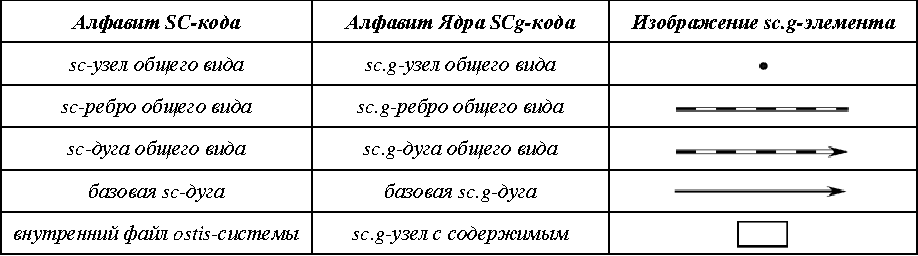
\includegraphics{figures/intro/scg/SCg-core-alphabet.pdf}\\}

%TODO сверить пропорции sc.g-элементов и изменить описание
\scnheader{sc.g-узел общего вида}
\scnidtf{\textit{sc.g-элемент}, являющийся графическим изображением \textit{sc-узла общего вида}}
\scnexplanation{Все \textit{sc-узлы}, не являющиеся знаками файлов, в тексте (конструкции) \textit{Ядра SCg-кода}, изображаются в виде небольших чёрных кругов одинакового диаметра, который обозначим через $\bm{d}$, и точная величина которого зависит от масштаба отображения \textit{sc.g-текста}.}

\scnheader{sc.g-ребро общего вида}
\scnidtf{\textit{sc.g-элемент}, являющийся графическим изображением \textit{sc-ребра общего вида}}
\scnexplanation{Каждое \textit{sc-ребро} в \textit{Ядре SCg-кода} изображается в виде широкой линии, в которой чередуются фрагменты со сплошной заливкой и без заливки, не имеющей самопересечений и имеющей общую толщину, равную примерно $\bm{0.7d}$.}

\scnheader{sc.g-дуга общего вида}
\scnidtf{\textit{sc.g-элемент}, являющийся графическим изображением \textit{sc-дуги общего вида}}
\scnexplanation{Каждая \textit{sc-дуга} в \textit{Ядре SCg-кода} изображается в виде широкой линии, в которой чередуются фрагменты со сплошной заливкой и без заливки, не имеющей самопересечений, имеющей общую толщину, равную примерно $\bm{0.7d}$ и имеющей изображение стрелочки на одном из концов этой линии.}

\scnheader{базовая sc.g-дуга}
\scnidtf{\textit{sc.g-элемент}, являющийся графическим изображением \textit{базовой sc-дуги}}
\scnexplanation{Каждая входящая в состав sc-текста \textit{базовая sc-дуга} в \textit{Ядре SCg-кода} изображается в виде линии произвольной формы, не имеющий самопересечений, имеющий толщину $\bm{0.4d}$, и имеющей изображение стрелочки на одном из ее концов.}

\scnheader{внутренний файл ostis-системы}
\scnidtf{sc-узел с содержимым}
\scnaddlevel{1}
\scniselement{часто используемый sc-идентификатор}
\scnaddlevel{-1}
\scnidtf{sc-узел, являющийся знаком внутреннего файла ostis-системы}
\scnidtf{sc-знак внутреннего файла ostis-системы}

\scnheader{sc.g-узел с содержимым}
\scnidtf{sc.g-узел, имеющий содержимое}
\scnidtf{sc.g-узел, являющийся знаком внутреннего файла ostis-системы}
\scnidtf{sc.g-знак внутреннего файла ostis-системы}
\scnidtf{sc.g-рамка, ограничивающая изображение (представление) внутреннего файла ostis-системы, обозначаемого этой sc.g-рамкой}
\scnidtf{sc.g-рамка}
\scnaddlevel{1}
\scnnote{\textit{sc.g-рамка} -- это всегда прямоугольник, максимальный размер которого не ограничивается, но минимальный фиксируется и соответствует \textit{sc.g-рамке}, внутри которой обозначаемый ею \textit{файл} не отображается.}
\scnaddlevel{-1}
\scnexplanation{Каждый входящий в sc-текст \textit{sc-узел, имеющий содержимое}, в \textit{Ядре SCg-кода} изображается в виде прямоугольника произвольного размера с толщиной линии $\bm{0.6d}$. Внутри этого прямоугольника отображается \textit{файл}, обозначаемый изображаемым \textit{sc-узлом}. Если нет необходимости изображать в тексте сам \textit{файл}, то \textit{sc-узел}, обозначающий такой \textit{файл}, в \textit{sc.g-тексте} изображается в виде прямоугольника со сторонами $\bm{2d}$ по вертикали и $\bm{4d}$ по горизонтали.}

\scnheader{Алфавит Ядра SCg-кода}
\scnnote{Трудно сразу поверить, что на основе такого простого алфавита можно построить удобный и \uline{универсальный} графовый язык. В рамках \textit{Документации Технологии OSTIS} мы постараемся Вас в этом убедить. Кроме того, нас не должна настораживать простота алфавита, поскольку человечество имеет большой опыт кодирования, хранения в памяти и передачи по каналам связи самых различных информационных ресурсов, используя алфавит, состоящий только из двух классов элементов -- единиц и нулей. 

Мы ведем речь о принципиально ином (графовом) способе кодирования информации в \textit{компьютерных системах}, но стараемся при этом свести это кодирование к достаточно простому алфавиту хотя бы для того, чтобы искусственно не усложнять проблему создания нового поколения компьютеров, основанных на указанном способе кодирования информации. 

Расширения \textit{Ядра SCg-кода} рассмотрим как направления перехода от текстов \textit{Ядра SCg-кода} к более компактным текстам. Но, поскольку это приводит к усложнению \textit{Синтаксиса SCg-кода} и, в первую очередь, к расширению \textit{Алфавита SCg-кода}, делать такие расширения необходимо обоснованно с учетом частоты встречаемости в рамках \textit{баз знаний ostis-систем} соответствующих фрагментов.}

\bigskip
\scnendstruct \scnendsegmentcomment{Описание Ядра SCg-кода}

\scnsegmentheader{Описание Первого направления расширения Ядра SCg-кода}
\scnstartsubstruct

\scnheader{Первое направление расширения Ядра SCg-кода}

\scnexplanation{\textit{Первое направление синтаксического расширения Ядра SCg-кода} -- это \uline{приписывание} некоторым \mbox{sc.g-элементам} \textit{основных sc-идентификаторов*} (чаще всего - строковых идентификаторов, то есть имен) \textit{sc-элементов} , изображаемых этими \textit{sc.g-элементами}. Указываемые идентификаторы являются уникальным для каждого идентифицируемого (именуемого) \textit{sc.g-элемента}. Приписывание \textit{sc.g-элементам} уникальных идентификаторов дает возможность в рамках одного \textit{sc.g-текста} дублировать (копировать) некоторые \textit{sc.g-узлы} при условии, если \uline{всем} таким копиям будут приписаны соответствующие идентификаторы. Такое дублирование \textit{sc.g-узлов} является дополнительным средствам \uline{наглядного} размещения \textit{sc.g-текстов}. Кроме того, приписывание \textit{sc.g-элементу} соответствующего ему основного (уникального) \textit{sc-идентификатора*} представляет собой более компактный вариант изображения \textit{sc.g-текстов}.}

\newpage
\scnheader{Пример sc.g-текста, трансформируемого по Первому направлению расширения Ядра SCg-кода}
\scneqscg{figures/intro/scg/scg_transf1.png}
\scniselement{sc.g-текст}
\scnexplanation{Здесь (в левом нижнем углу приведенного sc.g-текста) представлен \textit{sc.g-узел общего вида}, изображающий \textit{sc-узел общего вида}, которому соответствует \textit{основной sc-идентификатор*} в виде строки ``\textbf{\textit{ei}}''}
\scnrelfrom{трансформация sc.g-текста по Первому направлению расширения Ядра SCg-кода}{\scnfilescg{figures/intro/scg/scg_transf2.png}}
\scnaddlevel{1}
    \scniselement{sc.g-текст}
    \scnexplanation{\textit{sc.g-узлу общего вида} изображающему \textit{sc-узел}, внешним идентификатором которого является строка ``\textit{основной sc-идентификатор*}'' и который, соответственно является знаком \textit{бинарного ориентированного отношения}, каждая \textit{пара} которого связывает идентифицируемый \textit{sc-элемент} с его основным внешним sc-идентификатором, приписывается указанный внешний идентификатор изображаемого им \textit{sc-элемента}.}
    \scnrelfrom{трансформация sc.g-текста по Первому направлению расширения Ядра SCg-кода}{\scnfilescg{figures/intro/scg/scg_transf3.png}}
    \scnaddlevel{1}
        \scniselement{sc.g-текст} 
        \scnexplanation{В результате данной трансформации исходный \mbox{\textit{sc.g-текст}} трансформируется в один \textit{sc.g-общего вида}, которому приписывается \textit{основной sc-идентификатор} ``\textit{\textbf{ei}}''.}
    \scnaddlevel{-1}
\scnaddlevel{-1}


\scnheader{трансформация sc.g-текста по Первому направлению расширения Ядра SCg-кода*}
\scnidtf{Бинарное ориентированное отношение, каждая пара которого связывает исходный вид трансформируемого sc.g-текста и результат этой трансформации}
\scnnote{Подчеркнем, что рассматриваемая трансформация преобразует исходный текст Ядра \textit{SCg-кода} в текст, семантически эквивалентный, но принадлежащий не Ядру \textit{SCg-кода}, а его расширению.
}

\scnheader{синтаксическая трансформация*}
\scnidtf{синтаксическая трансформация информационной конструкции*}
\scnsuperset{синтаксическая трансформация sc.g-текста*}
\scnaddlevel{1}
\scnsuperset{трансформация sc.g-текста по Первому направлению расширения Ядра SCg-кода*}
\scnaddlevel{-1}

\bigskip
\scnendstruct \scnendsegmentcomment{Описание первого направления расширения Ядра SCg-кода}

\newpage
\scnsegmentheader{Описание Второго направления расширения Ядра SCg-кода}
\scnstartsubstruct

\scnheader{Второе направление расширения Ядра SCg-кода}
\scnexplanation{\textit{Второе направление расширения Ядра SCg-кода} -- это уточнение типологии \textit{константных постоянных сущностей} и расширение \textit{Алфавита Ядра SCg-кода}, позволяющее типологию \textit{константных постоянных сущностей} привести в соответствие с синтаксической типологией новых вводимых элементов \textit{Алфавита SCg-кода}. Рассмотрим подробнее sc.g-элементы, знаки \textit{константных постоянных сущностей} различного вида. Графическим признаком \textit{константных постоянных sc-узлов} в конструкциях SCg-кода является их изображение в виде \uline{окружностей} диаметра $3d$, где $d$ -- диаметр sc.g-узла общего вида. Такое изображение является более компактной записью факта принадлежности заданного sc-узла (назовем его $\bm{vi}$) классу sc-констант и классу обозначений постоянных сущностей. Запись этого факта в \textit{Ядре SCg-кода} потребует (1) явного изображения sc-узла, обозначающего класс всевозможных константных sc-элементов (класс \textit{sc-констант}), (2) явного изображения базовой sc-дуги, соединяющего изображение sc-узла, обозначающего класс sc-констант, с изображением заданного константного sc-узла, (3) явного изображение sc-узла, обозначающего класс всевозможных sc-элементов, обозначающих \textit{постоянные сущности}, (4) явного изображения базовой sc-дуги, соединяющего изображение sc-узла, обозначающего класс обозначений \textit{постоянных сущностей} с изображением рассматриваемого sc-узла $\bm{vi}$ (Смотрите \textit{Файл. Изображение спецификации sc.g-элемента средствами Ядра SCg-кода и Первого расширения Ядра SCg-кода}).

Общепринятая запись данного факта выглядит следующим образом:

``\textit{sc-константа} $\ni \bm{vi}$; \textit{постоянная сущность} $\ni \bm{v_i};$''

\textit{Константные постоянные sc-ребра} в конструкциях SCg-кода изображаются в виде двойной линии, каждая из которых имеет толщину примерно $d/7$, а расстояние между ними равно примерно $3d/7$. 

\textit{Константные постоянные sc-дуги} изображаются в виде такой же двойной линии, но со стрелочкой. Все \textit{базовые sc-дуги}, а также все sc-узлы, имеющие содержимое, по определению являются \textit{константными постоянными sc-элементами}. 

\textit{Константные sc.g-узлы}, изображаемые окружностями диаметра $3d$ и толщиной границы $d/5$, обозначают \textit{константные постоянные сущности}, о которых мало что известно, но известно то, что они не являются парами (то есть множествами, \textit{мощность*} которых равна 2) и, следовательно, не могут быть изображёны в виде sc.g-дуг или sc.g-рёбер. Но, если при этом об обозначаемой \textit{константной постоянной сущности} ($\bm{vi}$) известно, что она является классом сущностей, то явное указание принадлежности sc-элемента \textit{vi} всевозможных классов можно заменить на специальное графическое изображение sc-элемента \textit{vi}, предполагаемое указанную принадлежность. Это приводит к расширению  \textit{Алфавита SCg-кода} (см. \textit{Примеры sc.g-текстов, трансформируемых по Второму направлению расширения Ядра SCg-код}).

Аналогичным образом (см. \textit{Примеры sc.g-текстов, трансформируемых по Второму направлению расширения Ядра SCg-код}) вводятся: 
\begin{scnitemize}
\item sc.g-узел, являющийся изображением \textit{класса};  
\item sc.g-узел, являющийся изображением \textit{класса классов};  
\item sc.g-узел, являющийся изображением \textit{отношения}; 
\item sc.g-узел, являющийся изображением \textit{ролевого отношения}; 
\item sc.g-узел, являющийся изображением \textit{структуры};  
\item sc.g-узел, являющийся изображением \textit{небинарной связки};
\item sc.g-узел, являющийся изображением \textit{первичной сущности} (терминальной сущности, которая не является множеством, а также файлом, хранимым в памяти ostis-системы).
\end{scnitemize}

Важное место среди константных постоянных сущностей занимают \textit{константные постоянные пары принадлежности}, обозначаемое соответствующими \textit{sc.g-дугами}. Такие пары принадлежности и обозначающие их sc.g-дуги бывают позитивными, негативными и нечеткими. Константная постоянная позитивная sc.g-дуга принадлежности есть ничто иное, как \textit{базовая sc.g-дуга}. Константная постоянная негативная sc.g-дуга принадлежности изображается в виде \textit{базовой sc.g-дуги}, перечеркнутой штриховыми черточками. Константная постоянная нечёткая sc.g-дуга принадлежности изображается в виде "недочеркнутой"{} \textit{базовой sc.g-дуги}, с каждой стороны которой отображаются штрихи, по длине равные половине от длины штрихов, которыми перечеркнута \textit{константная постоянная негативная sc.g-дуга}.}

\scnheader{Файл. Изображение спецификации sc.g-элемента средствами Ядра SCg-кода и Второго направления расширения Ядра SCg-кода}
\scneqscg{figures/intro/scg/scg2ex.png}

\scnheader{Примеры sc.g-текстов, трансформируемых по Второму направлению расширения Ядра SCg-кода}
\scnstructinclusion

\scnmakeset{\scgfileitem{figures/intro/scg/scg2_ex1.png}\\
\scnaddlevel{1}
    \scnrelfrom{синтаксическая трансформация}{\scnfilescg{figures/intro/scg/scg2_ex1_1.png}}
    \scnaddlevel{1}
        \scnexplanation{Здесь вводится новый синтаксический вид \textit{sc.g-элементов} -- \textit{константный постоянный sc.g-узел общего вида}, изображаемый окружностью диаметра $3d$ и толщиной границы $d/5$.}
    \scnaddlevel{-1}
\scnaddlevel{-1};
\scgfileitem{figures/intro/scg/nodes/const_perm/scg_const_perm_class1.png}\\
\scnaddlevel{1}
    \scnrelfrom{синтаксическая трансформация}{\scnfilescg{figures/intro/scg/nodes/const_perm/scg_const_perm_class2.png}}
    \scnaddlevel{1}
        \scnexplanation{Здесь вводится новый синтаксический вид \textit{sc.g-элементов} -- \textit{константный постоянный sc.g-узел, обозначающий класс}, изображаемый как \textit{константный постоянный sc.g-узел} с "решеткой"{} внутри.}
    \scnaddlevel{-1}
\scnaddlevel{-1}
\newpage;
\scgfileitem{figures/intro/scg/nodes/const_perm/scg_const_perm_class_of_classes1.png}\\
\scnaddlevel{1}
    \scnrelfrom{синтаксическая трансформация}{\scnfilescg{figures/intro/scg/nodes/const_perm/scg_const_perm_class_of_classes2.png}}
    \scnaddlevel{1}
        \scnexplanation{Здесь вводится новый синтаксический вид \textit{sc.g-элементов} -- \textit{константный постоянный \mbox{sc.g-узел}, обозначающий класс классов}, изображаемый как \textit{константный постоянный \mbox{sc.g-узел}} с направленным вверх углом внутри.}
    \scnaddlevel{-1}
\scnaddlevel{-1};
\scgfileitem{figures/intro/scg/nodes/const_perm/scg_const_perm_norole1.png}\\
\scnaddlevel{1}
    \scnrelfrom{синтаксическая трансформация}{\scnfilescg{figures/intro/scg/nodes/const_perm/scg_const_perm_norole2.png}}
    \scnaddlevel{1}
        \scnexplanation{Здесь вводится новый синтаксический вид \textit{sc.g-элементов} -- \textit{константный постоянный \mbox{sc.g-узел}, обозначающий неролевое отношение}, изображаемый как \textit{константный постоянный sc.g-узел} с "крестиком"{} внутри.}
    \scnaddlevel{-1}
\scnaddlevel{-1};
\scgfileitem{figures/intro/scg/nodes/const_perm/scg_const_perm_role1.png}\\
\scnaddlevel{1}
    \scnrelfrom{синтаксическая трансформация}{\scnfilescg{figures/intro/scg/nodes/const_perm/scg_const_perm_role2.png}}
    \scnaddlevel{1}
        \scnexplanation{Здесь вводится новый синтаксический вид \textit{sc.g-элементов} -- \textit{константный постоянный sc.g-узел, обозначающий ролевое отношение}, изображаемый как \textit{константный постоянный sc.g-узел} с "плюсом"{} внутри.}
    \scnaddlevel{-1}
\scnaddlevel{-1}
\newpage;
\scgfileitem{figures/intro/scg/nodes/const_perm/scg_const_perm_structure1.png}\\
\scnaddlevel{1}
    \scnrelfrom{синтаксическая трансформация}{\scnfilescg{figures/intro/scg/nodes/const_perm/scg_const_perm_structure2.png}}
    \scnaddlevel{1}
        \scnexplanation{Здесь вводится новый синтаксический вид \textit{sc.g-элементов} -- \textit{константный постоянный \mbox{sc.g-узел}, обозначающий структуру}, изображаемый как \textit{константный постоянный \mbox{sc.g-узел}} с точкой внутри.}
    \scnaddlevel{-1}
\scnaddlevel{-1};
\scgfileitem{figures/intro/scg/nodes/const_perm/scg_const_perm_primary_entity1.png}\\
\scnaddlevel{1}
    \scnrelfrom{синтаксическая трансформация}{\scnfilescg{figures/intro/scg/nodes/const_perm/scg_const_perm_primary_entity2.png}}
    \scnaddlevel{1}
        \scnexplanation{Здесь вводится новый синтаксический вид \textit{sc.g-элементов} -- \textit{константный постоянный \mbox{sc.g-узел}, обозначающий первичную сущность}, изображаемый как \textit{константный постоянный \mbox{sc.g-узел}} с  косой штриховкой внутри.}
    \scnaddlevel{-1}
\scnaddlevel{-1};
\scgfileitem{figures/intro/scg/nodes/const_perm/scg_const_perm_tuple1.png}\\
\scnaddlevel{1}
    \scnrelfrom{синтаксическая трансформация}{\scnfilescg{figures/intro/scg/nodes/const_perm/scg_const_perm_tuple2.png}}
    \scnaddlevel{1}
        \scnexplanation{Здесь вводится новый синтаксический вид \textit{sc.g-элементов} -- \textit{константный постоянный \mbox{sc.g-узел}, обозначающий небинарную связку}, изображаемый как \textit{константный постоянный sc.g-узел} с горизонтальной линией внутри.}
    \scnaddlevel{-1}
\scnaddlevel{-1}
\newpage;
\scgfileitem{figures/intro/scg/arcs/const/scg_const_perm_noorien1.png}\\
\scnaddlevel{1}
    \scnrelfrom{синтаксическая трансформация}{\scnfilescg{figures/intro/scg/arcs/const/scg_const_perm_noorien2.png}}
    \scnaddlevel{1}
        \scnexplanation{Здесь вводится новый синтаксический вид \textit{sc.g-элементов} -- \textit{константное постоянное sc.g-ребро}, изображаемое двумя непрерывными параллельными линиями.}
    \scnaddlevel{-1}
\scnaddlevel{-1};
\scgfileitem{figures/intro/scg/arcs/const/scg_const_perm_orient1.png}\\
\scnaddlevel{1}
    \scnrelfrom{синтаксическая трансформация}{\scnfilescg{figures/intro/scg/arcs/const/scg_const_perm_orient2.png}}
    \scnaddlevel{1}
        \scnexplanation{Здесь вводится новый синтаксический вид \textit{sc.g-элементов} -- \textit{константная постоянная \mbox{sc.g-дуга}}, изображаемая двумя непрерывными параллельными линиями с общей стрелкой на одном из концов.}
    \scnaddlevel{-1}
\scnaddlevel{-1};
\scgfileitem{figures/intro/scg/arcs/const/scg_const_perm_positive1.png}\\
\scnaddlevel{1}
    \scnrelfrom{синтаксическая трансформация}{\scnfilescg{figures/intro/scg/arcs/const/scg_const_perm_positive2.png}}
    \scnaddlevel{1}
        \scnexplanation{\textit{Константная постоянная позитивная sc.g-дуга принадлежности} есть ничто иное, как \textit{базовая sc.g-дуга}.}
    \scnaddlevel{-1}
\scnaddlevel{-1}
\newpage;
\scgfileitem{figures/intro/scg/arcs/const/scg_const_perm_negative1.png}\\
\scnaddlevel{1}
    \scnrelfrom{синтаксическая трансформация}{\scnfilescg{figures/intro/scg/arcs/const/scg_const_perm_negative2.png}}
    \scnaddlevel{1}
        \scnexplanation{Здесь вводится новый синтаксический вид \textit{sc.g-элементов} -- \textit{константная постоянная негативная sc.g-дуга принадлежности}, изображается в виде \textit{базовой sc.g-дуги}, перечеркнутой штриховыми черточками.}
    \scnaddlevel{-1}
\scnaddlevel{-1};
\scgfileitem{figures/intro/scg/arcs/const/scg_const_perm_fuzzy1.png}\\
\scnaddlevel{1}
    \scnrelfrom{синтаксическая трансформация}{\scnfilescg{figures/intro/scg/arcs/const/scg_const_perm_fuzzy2.png}}
    \scnaddlevel{1}
        \scnexplanation{Здесь вводится новый синтаксический вид \textit{sc.g-элементов} -- \textit{константная постоянная нечеткая sc.g-дуга принадлежности}, которая изображается в виде "недочеркнутой"{} \textit{базовой sc.g-дуги}, с каждой стороны которой отображаются штрихи, по длине равные половине от длины штрихов, которыми перечеркнута \textit{константная постоянная негативная sc.g-дуга}.}
    \scnaddlevel{-1}
\scnaddlevel{-1}
}

\newpage
\scnheader{Примеры sc.g-текста, записанного средствами Второго направления расширения Ядра SCg-кода}
\scnstructinclusion

\scnmakeset{\scgfileitem{figures/intro/scg/examples/scg_example_triangle.png}
\scnaddlevel{1}
\scniselementrole{пример}{sc.g-текст}
\scnexplanation{Данный sc.g-текст содержит следующую информацию:
\begin{scnitemize}
\item Сущности \textit{Треугольник ABC}~~ и ~~\textit{Треугольник CDE} являются треугольниками (принадлежат классу \textit{треугольников}). При этом известно, что площадь \textit{Треугольника CDE} в 4 раза больше, чем площадь \textit{Треугольника ABC}, но конкретные значения ллощадей не известны\char59
\item Сущность \textit{Отрезок DE} является отрезком (принадлежит классу \textit{отрезков}) и является стороной \textit{Треугольника CDE}. Кроме того, у \textit{Отрезка DE} есть длина, измерение которой в сантиметрах составляет 5. Обратите внимание, что в данном случае для упрощения понимания использовано бинарное отношение \textit{длина*}, которое является \textit{неосновным понятием} и в базе знаний заменяется на \textit{базовую sc-дугу}, связывающую величину как класс эквивалентности с конкретной сущностью, входящей в данный класс, в данном случае -- \textit{Отрезок DE}\char59  
\item Сущность \textit{Треугольник AEB} является треугольником и имеет \textit{внутренний угол*}~~~ \textit{Угол AEB}. В свою очередь, \textit{Угол AEB} является \textit{углом} и имеет \textit{косинус*}, равный 0,5\char59
\item \textit{Треугольник AEB} имеет \textit{сторону*} (не указывается, какая именно из сторон имеется в виду), \textit{средней точкой*} которой является \textit{Точка O}. В свою очередь, \textit{Точка O} является центром некоторой \textit{Окружности O}, которая относится к классу \textit{окружностей}.
\end{scnitemize}
}\scnaddlevel{-1}
\newpage;
\scgfileitem{figures/intro/scg/examples/scg_example_alice.png}
\newpage
\scnaddlevel{1}
	\scnexplanation{Данный sc.g-текст основан на популярном примере, наглядно иллюстрируещем понятие семантической сети, известном как ``Социальная сеть Алисы''. Как видно из примера, данный текст описывает различные взаимосвязи персоны по имени Алиса, при этом некоторые из используемых отношений является ориентированными (например, ``работник*''), а некоторые -- неориентированными (например, ``друг*'').}
\scnaddlevel{-1}
}

\bigskip
\scnendstruct \scnendsegmentcomment{Описание Второго направления расширения Ядра SCg-кода}

\scnsegmentheader{Описание Третьего направления расширения Ядра SCg-кода}

\scnstartsubstruct

\scnheader{Третье направление расширения Ядра SCg-кода}
\scnexplanation{\textit{Третье направление расширения Ядра SCg-кода} -- это расширение его алфавита путем введения дополнительных sc.g-элементов, обозначающих \textit{константные временные сущности} различного вида. Признаком sc.g-элементов, обозначающих \textit{константные временные сущности} являются точечные линии (линии, состоящие из точек, размер которых равен размеру изображаемой линии и которые близко расположены друг к другу на расстоянии, равном половине их размера), с помощью которых рисуются окружности при изображении sc-узлов, а также линии при изображении sc-коннекторов.

Результатом \textit{Третьего направления расширения Ядра SCg-кода} является введение следующих видов sc.g-элементов (см. \textit{Примеры sc.g-текстов, трансформируемых по Третьему направлению расширения Ядра SCg-кода}).}

\scnheader{Примеры sc.g-текстов, трансформируемых по Третьему направлению расширения Ядра SCg-кода}
\scnstructinclusion
\scnmakeset{\scgfileitem{figures/intro/scg/nodes/const_temp/scg_const_temp_general_view1.png}\\
\scnaddlevel{1}
    \scnrelfrom{синтаксическая трансформация}{\scnfilescg{figures/intro/scg/nodes/const_temp/scg_const_temp_general_view2.png}}
    \scnaddlevel{1}
        \scnexplanation{Здесь вводится новый синтаксический вид \textit{sc.g-элементов} -- \textit{константный временный \mbox{sc.g-узел общего вида}}, изображаемый точечной окружностью диаметра $3d$ и толщиной границы $d/5$.}
    \scnaddlevel{-1}
\scnaddlevel{-1};
\scgfileitem{figures/intro/scg/nodes/const_temp/scg_const_temp_class1.png}\\
\scnaddlevel{1}
    \scnrelfrom{синтаксическая трансформация}{\scnfilescg{figures/intro/scg/nodes/const_temp/scg_const_temp_class2.png}}
    \scnaddlevel{1}
        \scnexplanation{Здесь вводится новый синтаксический вид \textit{sc.g-элементов} -- \textit{константный временный \mbox{sc.g-узел}, обозначающий класс}, изображаемый как \textit{константный временный \mbox{sc.g-узел}} с "решеткой"{} внутри.}
    \scnaddlevel{-1}
\scnaddlevel{-1};
\scgfileitem{figures/intro/scg/nodes/const_temp/scg_const_temp_class_of_classes1.png}\\
\scnaddlevel{1}
    \scnrelfrom{синтаксическая трансформация}{\scnfilescg{figures/intro/scg/nodes/const_temp/scg_const_temp_class_of_classes2.png}}
    \scnaddlevel{1}
        \scnexplanation{Здесь вводится новый синтаксический вид \textit{sc.g-элементов} -- \textit{константный временный \mbox{sc.g-узел}, обозначающий класс классов}, изображаемый как \textit{константный временный \mbox{sc.g-узел}} с направленным вверх углом внутри.}
    \scnaddlevel{-1}
\scnaddlevel{-1};
\scgfileitem{figures/intro/scg/nodes/const_temp/scg_const_temp_norole1.png}\\
\scnaddlevel{1}
    \scnrelfrom{синтаксическая трансформация}{\scnfilescg{figures/intro/scg/nodes/const_temp/scg_const_temp_norole2.png}}
    \scnaddlevel{1}
        \scnexplanation{Здесь вводится новый синтаксический вид \textit{sc.g-элементов} -- \textit{константный временный \mbox{sc.g-узел}, обозначающий неролевое отношение}, изображаемый как \textit{константный временный sc.g-узел} с "крестиком"{} внутри.}
    \scnaddlevel{-1}
\scnaddlevel{-1};
\scgfileitem{figures/intro/scg/nodes/const_temp/scg_const_temp_role1.png}\\
\scnaddlevel{1}
    \scnrelfrom{синтаксическая трансформация}{\scnfilescg{figures/intro/scg/nodes/const_temp/scg_const_temp_role2.png}}
    \scnaddlevel{1}
    \newpage
        \scnexplanation{Здесь вводится новый синтаксический вид \textit{sc.g-элементов} -- \textit{константный временный \mbox{sc.g-узел}, обозначающий ролевое отношение}, изображаемый как \textit{константный временный \mbox{sc.g-узел}} с "плюсом"{} внутри.}
    \scnaddlevel{-1}
\scnaddlevel{-1};
\scgfileitem{figures/intro/scg/nodes/const_temp/scg_const_temp_structure1.png}\\
\scnaddlevel{1}
    \scnrelfrom{синтаксическая трансформация}{\scnfilescg{figures/intro/scg/nodes/const_temp/scg_const_temp_structure2.png}}
    \scnaddlevel{1}
        \scnexplanation{Здесь вводится новый синтаксический вид \textit{sc.g-элементов} -- \textit{константный временный \mbox{sc.g-узел}, обозначающий структуру}, изображаемый как \textit{константный временный \mbox{sc.g-узел}} с точкой внутри.}
    \scnaddlevel{-1}
\scnaddlevel{-1};
\scgfileitem{figures/intro/scg/nodes/const_temp/scg_const_temp_primary_entity1.png}\\
\scnaddlevel{1}
    \scnrelfrom{синтаксическая трансформация}{\scnfilescg{figures/intro/scg/nodes/const_temp/scg_const_temp_primary_entity2.png}}
    \scnaddlevel{1}
        \scnexplanation{Здесь вводится новый синтаксический вид \textit{sc.g-элементов} -- \textit{константный временный \mbox{sc.g-узел}, обозначающий первичную сущность}, изображаемый как \textit{константный временный \mbox{sc.g-узел}} с косой штриховкой внутри.}
    \scnaddlevel{-1}
\scnaddlevel{-1};
\scgfileitem{figures/intro/scg/nodes/const_temp/scg_const_temp_tuple1.png}\\
\scnaddlevel{1}
    \scnrelfrom{синтаксическая трансформация}{\scnfilescg{figures/intro/scg/nodes/const_temp/scg_const_temp_tuple2.png}}
    \scnaddlevel{1}
    \newpage
        \scnexplanation{Здесь вводится новый синтаксический вид \textit{sc.g-элементов} -- \textit{константный временный \mbox{sc.g-узел}, обозначающий небинарную связку}, изображаемый как \textit{константный временный \mbox{sc.g-узел}} с горизонтальной линией внутри.}
    \scnaddlevel{-1}
\scnaddlevel{-1};
\scgfileitem{figures/intro/scg/arcs/const/scg_const_temp_noorien1.png}\\
\scnaddlevel{1}
    \scnrelfrom{синтаксическая трансформация}{\scnfilescg{figures/intro/scg/arcs/const/scg_const_temp_noorien2.png}}
    \scnaddlevel{1}
        \scnexplanation{Здесь вводится новый синтаксический вид \textit{sc.g-элементов} -- \textit{константное временное \mbox{sc.g-ребро}}, изображаемое двумя точечными параллельными линиями.}
    \scnaddlevel{-1}
\scnaddlevel{-1};
\scgfileitem{figures/intro/scg/arcs/const/scg_const_temp_orient1.png}\\
\scnaddlevel{1}
    \scnrelfrom{синтаксическая трансформация}{\scnfilescg{figures/intro/scg/arcs/const/scg_const_temp_orient2.png}}
    \scnaddlevel{1}
        \scnexplanation{Здесь вводится новый синтаксический вид \textit{sc.g-элементов} -- \textit{константная временная \mbox{sc.g-дуга}}, изображаемая двумя точечными параллельными линиями с общей стрелкой на одном из концов.}
    \scnaddlevel{-1}
\scnaddlevel{-1};
\scgfileitem{figures/intro/scg/arcs/const/scg_const_temp_positive1.png}\\
\scnaddlevel{1}
    \scnrelfrom{синтаксическая трансформация}{\scnfilescg{figures/intro/scg/arcs/const/scg_const_temp_positive2.png}}
    \scnaddlevel{1}
    \newpage
        \scnexplanation{Здесь вводится новый синтаксический вид \textit{sc.g-элементов} -- \textit{константная временная позитивная sc.g-дуга принадлежности}, изображаемая точечной линией со стрелкой на конце.}
    \scnaddlevel{-1}
\scnaddlevel{-1};
\scgfileitem{figures/intro/scg/arcs/const/scg_const_temp_negative1.png}\\
\scnaddlevel{1}
    \scnrelfrom{синтаксическая трансформация}{\scnfilescg{figures/intro/scg/arcs/const/scg_const_temp_negative2.png}}
    \scnaddlevel{1}
        \scnexplanation{Здесь вводится новый синтаксический вид \textit{sc.g-элементов} -- \textit{константная временная негативная sc.g-дуга принадлежности}, изображаемая точечной линией, перечеркнутой штриховыми черточками, со стрелкой на конце.}
    \scnaddlevel{-1}
\scnaddlevel{-1};
\scgfileitem{figures/intro/scg/arcs/const/scg_const_temp_fuzzy1.png}\\
\scnaddlevel{1}
    \scnrelfrom{синтаксическая трансформация}{\scnfilescg{figures/intro/scg/arcs/const/scg_const_temp_fuzzy2.png}}
    \scnaddlevel{1}
        \scnexplanation{Здесь вводится новый синтаксический вид \textit{sc.g-элементов} -- \textit{константная временная нечеткая sc.g-дуга принадлежности}, которая изображается в виде "недочеркнутой"{} \textit{\textit{константной временной позитивная sc.g-дуги принадлежности}, с каждой стороны которой отображаются штрихи, по длине равные половине от длины штрихов, которыми перечеркнута \textit{константная постоянная негативная sc.g-дуга}.}
    \scnaddlevel{-1}
{-1}}}

\bigskip
\scnendstruct \scnendsegmentcomment{Описание Третьего направления расширения Ядра SCg-кода}

\scnsegmentheader{Описание Четвёртого направления расширения Ядра SCg-кода}

\scnstartsubstruct

\scnheader{Четвёртое направление расширения Ядра SCg-кода}
\scnexplanation{\textit{Четвёртое направление расширения Ядра SCg-кода} -- это расширение его алфавита путем введения дополнительных элементов, обозначающих \textit{переменные постоянные сущности} различного вида. Признаком sc.g-элементов, обозначающих сущности указанного класса, являются квадратики для изображения обозначений \textit{переменных постоянных сущностей}, не являющихся бинарными связями, а также пунктирные и штрих-пунктирные линии для изображения \textit{переменных постоянных бинарных связей}. 

Подчеркнем, что \textit{переменные постоянные сущности} могут отличаться друг от друга по характеру их \textit{области значений*}. Этими значениями в общем случае могут быть как \textit{константные постоянные сущности}, так и \textit{переменные постоянные сущности}. В любом случае, значение \textit{переменной сущности} является либо \textit{константной сущностью}, либо \textit{переменной сущностью}. Если каждое значение переменной является константой, то такую переменную будем называть \textit{переменной первого уровня}. Если каждое значение переменной является \textit{переменной первого уровня}, то такую переменную будем называть \textit{переменной второго уровня}. 

\textit{Переменная постоянная сущность первого уровня } (первичная sc-переменная), не являющаяся бинарной связью -- это переменная, каждым значением которой является \textit{константная постоянная сущность}, не являющаяся бинарной связью. Такая переменная изображается квадратиком, который ориентирован по вертикали и горизонтали. 

\textit{переменная постоянная сущность второго уровня} (вторичная sc-переменная), не являющаяся бинарной связью, изображается квадратиком, повернутым на 45$^\circ$. 

Указанная выше семантика таких изображений приписывается \uline{по умолчанию}. Это означает, что, если обозначаемая sc-переменная имеет более сложную структуру области её значений (является sc-переменной третьего и выше уровня или sc-переменной, значения которой имеют различный логический уровень), то эта область должна быть специфицирована явно, при этом такая sc-переменная в SCg-коде изображается так же, как первичная sc-переменная.}

\scnheader{Примеры sc.g-текстов, трансформируемых по Четвертому направлению расширения Ядра SCg-кода}
\scnstructinclusion
\scnmakeset{\scgfileitem{figures/intro/scg/nodes/var_perm/scg_var_perm_general_view1.png}\\
\scnaddlevel{1}
    \scnrelfrom{синтаксическая трансформация}{\scnfilescg{figures/intro/scg/nodes/var_perm/scg_var_perm_general_view2.png}}
    \scnaddlevel{1}
        \scnexplanation{Здесь вводится новый синтаксический вид \textit{sc.g-элементов} -- \textit{переменный постоянный \mbox{sc.g-узел} общего вида}, изображаемый квадратиком cj со стороной длины $3d$ и толщиной границы $d/5$.}
    \scnaddlevel{-1}
\scnaddlevel{-1};
\scgfileitem{figures/intro/scg/nodes/var_perm/scg_var_perm_class1.png}\\
\scnaddlevel{1}
    \scnrelfrom{синтаксическая трансформация}{\scnfilescg{figures/intro/scg/nodes/var_perm/scg_var_perm_class2.png}}
    \scnaddlevel{1}
        \scnexplanation{Здесь вводится новый синтаксический вид \textit{sc.g-элементов} -- \textit{переменный постоянный sc.g-узел, обозначающий класс}, изображаемый как \textit{переменный постоянный sc.g-узел} с "решеткой"{} внутри.}
    \scnaddlevel{-1}
\scnaddlevel{-1}
\newpage;
\scgfileitem{figures/intro/scg/nodes/var_perm/scg_var_perm_class_of_classes1.png}\\
\scnaddlevel{1}
    \scnrelfrom{синтаксическая трансформация}{\scnfilescg{figures/intro/scg/nodes/var_perm/scg_var_perm_class_of_classes2.png}}
    \scnaddlevel{1}
        \scnexplanation{Здесь вводится новый синтаксический вид \textit{sc.g-элементов} -- \textit{переменный постоянный \mbox{sc.g-узел}, обозначающий класс классов}, изображаемый как \textit{переменный постоянный \mbox{sc.g-узел}} с направленным вверх углом внутри.}
    \scnaddlevel{-1}
\scnaddlevel{-1};
\scgfileitem{figures/intro/scg/nodes/var_perm/scg_var_perm_norole1.png}\\
\scnaddlevel{1}
    \scnrelfrom{синтаксическая трансформация}{\scnfilescg{figures/intro/scg/nodes/var_perm/scg_var_perm_norole2.png}}
    \scnaddlevel{1}
        \scnexplanation{Здесь вводится новый синтаксический вид \textit{sc.g-элементов} -- \textit{переменный постоянный \mbox{sc.g-узел}, обозначающий неролевое отношение}, изображаемый как \textit{переменный постоянный \mbox{sc.g-узел}} с "крестиком"{} внутри.}
    \scnaddlevel{-1}
\scnaddlevel{-1};
\scgfileitem{figures/intro/scg/nodes/var_perm/scg_var_perm_role1.png}\\
\scnaddlevel{1}
    \scnrelfrom{синтаксическая трансформация}{\scnfilescg{figures/intro/scg/nodes/var_perm/scg_var_perm_role2.png}}
    \scnaddlevel{1}
        \scnexplanation{Здесь вводится новый синтаксический вид \textit{sc.g-элементов} -- \textit{переменный постоянный sc.g-узел, обозначающий ролевое отношение}, изображаемый как \textit{переменный постоянный sc.g-узел} с "плюсом"{} внутри.}
    \scnaddlevel{-1}
\scnaddlevel{-1}
\newpage;
\scgfileitem{figures/intro/scg/nodes/var_perm/scg_var_perm_structure1.png}\\
\scnaddlevel{1}
    \scnrelfrom{синтаксическая трансформация}{\scnfilescg{figures/intro/scg/nodes/var_perm/scg_var_perm_structure2.png}}
    \scnaddlevel{1}
        \scnexplanation{Здесь вводится новый синтаксический вид \textit{sc.g-элементов} -- \textit{переменный постоянный \mbox{sc.g-узел}, обозначающий структуру}, изображаемый как \textit{переменный постоянный \mbox{sc.g-узел}} с точкой внутри.}
    \scnaddlevel{-1}
\scnaddlevel{-1};
\scgfileitem{figures/intro/scg/nodes/var_perm/scg_var_perm_primary_entity1.png}\\
\scnaddlevel{1}
    \scnrelfrom{синтаксическая трансформация}{\scnfilescg{figures/intro/scg/nodes/var_perm/scg_var_perm_primary_entity2.png}}
    \scnaddlevel{1}
        \scnexplanation{Здесь вводится новый синтаксический вид \textit{sc.g-элементов} -- \textit{переменный постоянный \mbox{sc.g-узел}, обозначающий первичную сущность}, изображаемый как \textit{переменный постоянный \mbox{sc.g-узел}} с  косой штриховкой внутри.}
    \scnaddlevel{-1}
\scnaddlevel{-1};
\scgfileitem{figures/intro/scg/nodes/var_perm/scg_var_perm_tuple1.png}\\
\scnaddlevel{1}
    \scnrelfrom{синтаксическая трансформация}{\scnfilescg{figures/intro/scg/nodes/var_perm/scg_var_perm_tuple2.png}}
    \scnaddlevel{1}
        \scnexplanation{Здесь вводится новый синтаксический вид \textit{sc.g-элементов} -- \textit{переменный постоянный \mbox{sc.g-узел}, обозначающий небинарную связку}, изображаемый как \textit{переменный постоянный \mbox{sc.g-узел}} с горизонтальной линией внутри.}
    \scnaddlevel{-1}
\scnaddlevel{-1}
\newpage;
\scgfileitem{figures/intro/scg/arcs/var/scg_var_perm_noorien1.png}\\
\scnaddlevel{1}
    \scnrelfrom{синтаксическая трансформация}{\scnfilescg{figures/intro/scg/arcs/var/scg_var_perm_noorien2.png}}
    \scnaddlevel{1}
        \scnexplanation{Здесь вводится новый синтаксический вид \textit{sc.g-элементов} -- \textit{переменное постоянное \mbox{sc.g-ребро}}, изображаемое двумя пунктирными параллельными линиями.}
    \scnaddlevel{-1}
\scnaddlevel{-1};
\scgfileitem{figures/intro/scg/arcs/var/scg_var_perm_orient1.png}\\
\scnaddlevel{1}
    \scnrelfrom{синтаксическая трансформация}{\scnfilescg{figures/intro/scg/arcs/var/scg_var_perm_orient2.png}}
    \scnaddlevel{1}
        \scnexplanation{Здесь вводится новый синтаксический вид \textit{sc.g-элементов} -- \textit{переменная постоянная sc.g-дуга}, изображаемая двумя пунктирными параллельными линиями с общей стрелкой на одном из концов.}
    \scnaddlevel{-1}
\scnaddlevel{-1};
\scgfileitem{figures/intro/scg/arcs/var/scg_var_perm_positive1.png}\\
\scnaddlevel{1}
    \scnrelfrom{синтаксическая трансформация}{\scnfilescg{figures/intro/scg/arcs/var/scg_var_perm_positive2.png}}
    \scnaddlevel{1}
        \scnexplanation{\textit{переменная постоянная позитивная sc.g-дуга принадлежности}, изображаемая пунктирной линией со стрелкой на конце.}
    \scnaddlevel{-1}
\scnaddlevel{-1}
\newpage;
\scgfileitem{figures/intro/scg/arcs/var/scg_var_perm_negative1.png}\\
\scnaddlevel{1}
    \scnrelfrom{синтаксическая трансформация}{\scnfilescg{figures/intro/scg/arcs/var/scg_var_perm_negative2.png}}
    \scnaddlevel{1}
        \scnexplanation{Здесь вводится новый синтаксический вид \textit{sc.g-элементов} -- \textit{переменная постоянная негативная sc.g-дуга принадлежности}, изображается в виде \textit{переменной постоянной позитивной sc.g-дуги принадлежности}, перечеркнутой штриховыми черточками.}
    \scnaddlevel{-1}
\scnaddlevel{-1};
\scgfileitem{figures/intro/scg/arcs/var/scg_var_perm_fuzzy1.png}\\
\scnaddlevel{1}
    \scnrelfrom{синтаксическая трансформация}{\scnfilescg{figures/intro/scg/arcs/var/scg_var_perm_fuzzy2.png}}
    \scnaddlevel{1}
        \scnexplanation{Здесь вводится новый синтаксический вид \textit{sc.g-элементов} -- \textit{переменная постоянная нечеткая sc.g-дуга принадлежности}, которая изображается в виде "недочеркнутой"{} \textit{переменной постоянной позитивной sc.g-дуги принадлежности}, с каждой стороны которой отображаются штрихи, по длине равные половине от длины штрихов, которыми перечеркнута \textit{переменная постоянная негативная sc.g-дуга}.}
    \scnaddlevel{-1}
\scnaddlevel{-1};
\scgfileitem{figures/intro/scg/nodes/metavar_perm/scg_metavar_perm_general_view1.png}\\
\scnaddlevel{1}
    \scnrelfrom{синтаксическая трансформация}{\scnfilescg{figures/intro/scg/nodes/metavar_perm/scg_metavar_perm_general_view2.png}}
    \scnaddlevel{1}
        \scnexplanation{Здесь вводится новый синтаксический вид \textit{sc.g-элементов} -- \textit{метапеременный постоянный sc.g-узел общего вида}, изображаемый квадратиком, повернутым на 45 градусов.}
    \scnaddlevel{-1}
\scnaddlevel{-1}
\newpage;
\scgfileitem{figures/intro/scg/nodes/metavar_perm/scg_metavar_perm_class1.png}\\
\scnaddlevel{1}
    \scnrelfrom{синтаксическая трансформация}{\scnfilescg{figures/intro/scg/nodes/metavar_perm/scg_metavar_perm_class2.png}}
    \scnaddlevel{1}
        \scnexplanation{Здесь вводится новый синтаксический вид \textit{sc.g-элементов} -- \textit{метапеременный постоянный sc.g-узел, обозначающий класс}, изображаемый как \textit{метапеременный постоянный sc.g-узел} с "решеткой"{} внутри.}
    \scnaddlevel{-1}
\scnaddlevel{-1};
\scgfileitem{figures/intro/scg/nodes/metavar_perm/scg_metavar_perm_class_of_classes1.png}\\
\scnaddlevel{1}
    \scnrelfrom{синтаксическая трансформация}{\scnfilescg{figures/intro/scg/nodes/metavar_perm/scg_metavar_perm_class_of_classes2.png}}
    \scnaddlevel{1}
        \scnexplanation{Здесь вводится новый синтаксический вид \textit{sc.g-элементов} -- \textit{метапеременный постоянный sc.g-узел, обозначающий класс классов}, изображаемый как \textit{метапеременный постоянный sc.g-узел} с направленным вверх углом внутри.}
    \scnaddlevel{-1}
\scnaddlevel{-1};
\scgfileitem{figures/intro/scg/nodes/metavar_perm/scg_metavar_perm_norole1.png}\\
\scnaddlevel{1}
    \scnrelfrom{синтаксическая трансформация}{\scnfilescg{figures/intro/scg/nodes/metavar_perm/scg_metavar_perm_norole2.png}}
    \scnaddlevel{1}
        \scnexplanation{Здесь вводится новый синтаксический вид \textit{sc.g-элементов} -- \textit{метапеременный постоянный sc.g-узел, обозначающий неролевое отношение}, изображаемый как \textit{метапеременный постоянный sc.g-узел} с "крестиком"{} внутри.}
    \scnaddlevel{-1}
\scnaddlevel{-1}
\newpage;
\scgfileitem{figures/intro/scg/nodes/metavar_perm/scg_metavar_perm_role1.png}\\
\scnaddlevel{1}
    \scnrelfrom{синтаксическая трансформация}{\scnfilescg{figures/intro/scg/nodes/metavar_perm/scg_metavar_perm_role2.png}}
    \scnaddlevel{1}
        \scnexplanation{Здесь вводится новый синтаксический вид \textit{sc.g-элементов} -- \textit{метапеременный постоянный sc.g-узел, обозначающий ролевое отношение}, изображаемый как \textit{метапеременный постоянный sc.g-узел} с "плюсом"{} внутри.}
    \scnaddlevel{-1}
\scnaddlevel{-1};
\scgfileitem{figures/intro/scg/nodes/metavar_perm/scg_metavar_perm_structure1.png}\\
\scnaddlevel{1}
    \scnrelfrom{синтаксическая трансформация}{\scnfilescg{figures/intro/scg/nodes/metavar_perm/scg_metavar_perm_structure2.png}}
    \scnaddlevel{1}
        \scnexplanation{Здесь вводится новый синтаксический вид \textit{sc.g-элементов} -- \textit{метапеременный постоянный sc.g-узел, обозначающий структуру}, изображаемый как \textit{метапеременный постоянный \mbox{sc.g-узел}} с точкой внутри.}
    \scnaddlevel{-1}
\scnaddlevel{-1};
\scgfileitem{figures/intro/scg/nodes/metavar_perm/scg_metavar_perm_primary_entity1.png}\\
\scnaddlevel{1}
    \scnrelfrom{синтаксическая трансформация}{\scnfilescg{figures/intro/scg/nodes/metavar_perm/scg_metavar_perm_primary_entity2.png}}
    \scnaddlevel{1}
        \scnexplanation{Здесь вводится новый синтаксический вид \textit{sc.g-элементов} -- \textit{метапеременный постоянный sc.g-узел, обозначающий первичную сущность}, изображаемый как \textit{метапеременный постоянный sc.g-узел} с  косой штриховкой внутри.}
    \scnaddlevel{-1}
\scnaddlevel{-1}
\newpage;
\scgfileitem{figures/intro/scg/nodes/metavar_perm/scg_metavar_perm_tuple1.png}\\
\scnaddlevel{1}
    \scnrelfrom{синтаксическая трансформация}{\scnfilescg{figures/intro/scg/nodes/metavar_perm/scg_metavar_perm_tuple2.png}}
    \scnaddlevel{1}
        \scnexplanation{Здесь вводится новый синтаксический вид \textit{sc.g-элементов} -- \textit{метапеременный постоянный sc.g-узел, обозначающий небинарную связку}, изображаемый как \textit{метапеременный постоянный \mbox{sc.g-узел}} с горизонтальной линией внутри.}
    \scnaddlevel{-1}
\scnaddlevel{-1};
\scgfileitem{figures/intro/scg/arcs/meta/scg_metavar_perm_noorien1.png}\\
\scnaddlevel{1}
    \scnrelfrom{синтаксическая трансформация}{\scnfilescg{figures/intro/scg/arcs/meta/scg_metavar_perm_noorien2.png}}
    \scnaddlevel{1}
        \scnexplanation{Здесь вводится новый синтаксический вид \textit{sc.g-элементов} -- \textit{метапеременное постоянное sc.g-ребро}, изображаемое двумя штрих-пунктирными параллельными линиями.}
    \scnaddlevel{-1}
\scnaddlevel{-1};
\scgfileitem{figures/intro/scg/arcs/meta/scg_metavar_perm_orient1.png}\\
\scnaddlevel{1}
    \scnrelfrom{синтаксическая трансформация}{\scnfilescg{figures/intro/scg/arcs/meta/scg_metavar_perm_orient2.png}}
    \scnaddlevel{1}
        \scnexplanation{Здесь вводится новый синтаксический вид \textit{sc.g-элементов} -- \textit{метапеременная постоянная sc.g-дуга}, изображаемая двумя штрих-пунктирными непрерывными параллельными линиями с общей стрелкой на одном из концов.}
    \scnaddlevel{-1}
\scnaddlevel{-1}
\newpage;
\scgfileitem{figures/intro/scg/arcs/meta/scg_metavar_perm_positive1.png}\\
\scnaddlevel{1}
    \scnrelfrom{синтаксическая трансформация}{\scnfilescg{figures/intro/scg/arcs/meta/scg_metavar_perm_positive2.png}}
    \scnaddlevel{1}
        \scnexplanation{\textit{метапеременная постоянная позитивная sc.g-дуга принадлежности}, изображаемая штрих-пунктирной линией со стрелкой на конце.}
    \scnaddlevel{-1}
\scnaddlevel{-1};
\scgfileitem{figures/intro/scg/arcs/meta/scg_metavar_perm_negative1.png}\\
\scnaddlevel{1}
    \scnrelfrom{синтаксическая трансформация}{\scnfilescg{figures/intro/scg/arcs/meta/scg_metavar_perm_negative2.png}}
    \scnaddlevel{1}
        \scnexplanation{Здесь вводится новый синтаксический вид \textit{sc.g-элементов} -- \textit{метапеременная постоянная негативная sc.g-дуга принадлежности}, изображается в виде \textit{метапеременной постоянной позитивной sc.g-дуги принадлежности}, перечеркнутой штриховыми черточками.}
    \scnaddlevel{-1}
\scnaddlevel{-1};
\scgfileitem{figures/intro/scg/arcs/meta/scg_metavar_perm_fuzzy1.png}\\
\scnaddlevel{1}
    \scnrelfrom{синтаксическая трансформация}{\scnfilescg{figures/intro/scg/arcs/meta/scg_metavar_perm_fuzzy2.png}}
    \scnaddlevel{1}
        \scnexplanation{Здесь вводится новый синтаксический вид \textit{sc.g-элементов} -- \textit{метапеременная постоянная нечеткая sc.g-дуга принадлежности}, которая изображается в виде "недочеркнутой"{} \textit{метапеременной постоянной позитивной sc.g-дуги принадлежности}, с каждой стороны которой отображаются штрихи, по длине равные половине от длины штрихов, которыми перечеркнута \textit{метапеременная постоянная негативная sc.g-дуга}.}
    \scnaddlevel{-1}
\scnaddlevel{-1}
}

\bigskip
\scnendstruct \scnendsegmentcomment{Описание Четвёртого направления расширения Ядра SCg-кода}

\scnsegmentheader{Описание Пятого направления расширения Ядра SCg-кода}

\scnstartsubstruct

\scnheader{Пятое направление расширения Ядра SCg-кода}
\scnexplanation{\textit{Пятое направление расширения Ядра SCg-кода} -- это расширение его алфавита путем введения дополнительных \textit{sc.g-элементов}, обозначающих \textit{переменные временные сущности} различного вида. Указанные дополнительные \textit{sc.g-элементы} аналогичны тем, которые введены в рамках \textit{Четвертого направления расширения Ядра SCg-кода}, и отличаются только тем, что в \textit{Пятом направлении расширении Ядра SCg-кода} речь идёт о переменных \uline{временных} сущностях, а в \textit{Четвертом направлении расширения Ядра SCg-кода} -- о переменных \uline{постоянных} сущностях.}

\scnheader{Примеры sc.g-текстов, трансформируемых по Пятому направлению расширения Ядра SCg-кода}
\scnstructinclusion

\scnmakeset{\scgfileitem{figures/intro/scg/nodes/var_temp/scg_var_temp_general_view1.png}\\
\scnaddlevel{1}
    \scnrelfrom{синтаксическая трансформация}{\scnfilescg{figures/intro/scg/nodes/var_temp/scg_var_temp_general_view2.png}}
    \scnaddlevel{1}
        \scnexplanation{Здесь вводится новый синтаксический вид \textit{sc.g-элементов} -- \textit{переменный временный sc.g-узел общего вида}, изображаемый точечным квадратиком диаметра $3d$ и толщиной границы $d/5$.}
    \scnaddlevel{-1}
\scnaddlevel{-1};
\scgfileitem{figures/intro/scg/nodes/var_temp/scg_var_temp_class1.png}\\
\scnaddlevel{1}
    \scnrelfrom{синтаксическая трансформация}{\scnfilescg{figures/intro/scg/nodes/var_temp/scg_var_temp_class2.png}}
    \scnaddlevel{1}
        \scnexplanation{Здесь вводится новый синтаксический вид \textit{sc.g-элементов} -- \textit{переменный временный sc.g-узел, обозначающий класс}, изображаемый как \textit{переменный временный sc.g-узел} с "решеткой"{} внутри.}
    \scnaddlevel{-1}
\scnaddlevel{-1}
\newpage;
\scgfileitem{figures/intro/scg/nodes/var_temp/scg_var_temp_class_of_classes1.png}\\
\scnaddlevel{1}
    \scnrelfrom{синтаксическая трансформация}{\scnfilescg{figures/intro/scg/nodes/var_temp/scg_var_temp_class_of_classes2.png}}
    \scnaddlevel{1}
        \scnexplanation{Здесь вводится новый синтаксический вид \textit{sc.g-элементов} -- \textit{переменный временный \mbox{sc.g-узел}, обозначающий класс классов}, изображаемый как \textit{переменный временный sc.g-узел} с направленным вверх углом внутри.}
    \scnaddlevel{-1}
\scnaddlevel{-1};
\scgfileitem{figures/intro/scg/nodes/var_temp/scg_var_temp_norole1.png}\\
\scnaddlevel{1}
    \scnrelfrom{синтаксическая трансформация}{\scnfilescg{figures/intro/scg/nodes/var_temp/scg_var_temp_norole2.png}}
    \scnaddlevel{1}
        \scnexplanation{Здесь вводится новый синтаксический вид \textit{sc.g-элементов} -- \textit{переменный временный sc.g-узел, обозначающий неролевое отношение}, изображаемый как \textit{переменный временный sc.g-узел} с "крестиком"{} внутри.}
    \scnaddlevel{-1}
\scnaddlevel{-1};
\scgfileitem{figures/intro/scg/nodes/var_temp/scg_var_temp_role1.png}\\
\scnaddlevel{1}
    \scnrelfrom{синтаксическая трансформация}{\scnfilescg{figures/intro/scg/nodes/var_temp/scg_var_temp_role2.png}}
    \scnaddlevel{1}
        \scnexplanation{Здесь вводится новый синтаксический вид \textit{sc.g-элементов} -- \textit{переменный временный sc.g-узел, обозначающий ролевое отношение}, изображаемый как \textit{переменный временный sc.g-узел} с "плюсом"{} внутри.}
    \scnaddlevel{-1}
\scnaddlevel{-1}
\newpage;
\scgfileitem{figures/intro/scg/nodes/var_temp/scg_var_temp_structure1.png}\\
\scnaddlevel{1}
    \scnrelfrom{синтаксическая трансформация}{\scnfilescg{figures/intro/scg/nodes/var_temp/scg_var_temp_structure2.png}}
    \scnaddlevel{1}
        \scnexplanation{Здесь вводится новый синтаксический вид \textit{sc.g-элементов} -- \textit{переменный временный sc.g-узел, обозначающий структуру}, изображаемый как \textit{переменный временный sc.g-узел} с точкой внутри.}
    \scnaddlevel{-1}
\scnaddlevel{-1};
\scgfileitem{figures/intro/scg/nodes/var_temp/scg_var_temp_primary_entity1.png}\\
\scnaddlevel{1}
    \scnrelfrom{синтаксическая трансформация}{\scnfilescg{figures/intro/scg/nodes/var_temp/scg_var_temp_primary_entity2.png}}
    \scnaddlevel{1}
        \scnexplanation{Здесь вводится новый синтаксический вид \textit{sc.g-элементов} -- \textit{переменный временный sc.g-узел, обозначающий первичную сущность}, изображаемый как \textit{переменный временный sc.g-узел} с  косой штриховкой внутри.}
    \scnaddlevel{-1}
\scnaddlevel{-1};
\scgfileitem{figures/intro/scg/nodes/var_temp/scg_var_temp_tuple1.png}\\
\scnaddlevel{1}
    \scnrelfrom{синтаксическая трансформация}{\scnfilescg{figures/intro/scg/nodes/var_temp/scg_var_temp_tuple2.png}}
    \scnaddlevel{1}
        \scnexplanation{Здесь вводится новый синтаксический вид \textit{sc.g-элементов} -- \textit{переменный временный sc.g-узел, обозначающий небинарную связку}, изображаемый как \textit{переменный временный \mbox{sc.g-узел}} с горизонтальной линией внутри.}
    \scnaddlevel{-1}
\scnaddlevel{-1}
\newpage;
\scgfileitem{figures/intro/scg/arcs/var/scg_var_temp_noorien1.png}\\
\scnaddlevel{1}
    \scnrelfrom{синтаксическая трансформация}{\scnfilescg{figures/intro/scg/arcs/var/scg_var_temp_noorien2.png}}
    \scnaddlevel{1}
        \scnexplanation{Здесь вводится новый синтаксический вид \textit{sc.g-элементов} -- \textit{переменное временное sc.g-ребро}, изображаемое двумя пунктирными точечными параллельными линиями.}
    \scnaddlevel{-1}
\scnaddlevel{-1};
\scgfileitem{figures/intro/scg/arcs/var/scg_var_temp_orient1.png}\\
\scnaddlevel{1}
    \scnrelfrom{синтаксическая трансформация}{\scnfilescg{figures/intro/scg/arcs/var/scg_var_temp_orient2.png}}
    \scnaddlevel{1}
        \scnexplanation{Здесь вводится новый синтаксический вид \textit{sc.g-элементов} -- \textit{переменная временная sc.g-дуга}, изображаемая двумя пунктирными точечными параллельными линиями с общей стрелкой на одном из концов.}
    \scnaddlevel{-1}
\scnaddlevel{-1};
\scgfileitem{figures/intro/scg/arcs/var/scg_var_temp_positive1.png}\\
\scnaddlevel{1}
    \scnrelfrom{синтаксическая трансформация}{\scnfilescg{figures/intro/scg/arcs/var/scg_var_temp_positive2.png}}
    \scnaddlevel{1}
        \scnexplanation{\textit{Переменная временная позитивная sc.g-дуга принадлежности}, изображаемая в виде пунктирной точечной линией со стрелкой на конце.}
    \scnaddlevel{-1}
\scnaddlevel{-1}
\newpage;
\scgfileitem{figures/intro/scg/arcs/var/scg_var_temp_negative1.png}\\
\scnaddlevel{1}
    \scnrelfrom{синтаксическая трансформация}{\scnfilescg{figures/intro/scg/arcs/var/scg_var_temp_negative2.png}}
    \scnaddlevel{1}
        \scnexplanation{Здесь вводится новый синтаксический вид \textit{sc.g-элементов} -- \textit{переменная временная негативная sc.g-дуга принадлежности}, изображается в виде \textit{переменной временной позитивной sc.g-дуги}, перечеркнутой штриховыми черточками.}
    \scnaddlevel{-1}
\scnaddlevel{-1};
\scgfileitem{figures/intro/scg/arcs/var/scg_var_temp_fuzzy1.png}\\
\scnaddlevel{1}
    \scnrelfrom{синтаксическая трансформация}{\scnfilescg{figures/intro/scg/arcs/var/scg_var_temp_fuzzy2.png}}
    \scnaddlevel{1}
        \scnexplanation{Здесь вводится новый синтаксический вид \textit{sc.g-элементов} -- \textit{переменная временная нечеткая sc.g-дуга принадлежности}, которая изображается в виде "недочеркнутой"{} \textit{переменной временной позитивной sc.g-дуги}, с каждой стороны которой отображаются штрихи, по длине равные половине от длины штрихов, которыми перечеркнута \textit{переменная временная негативная sc.g-дуга}.}
    \scnaddlevel{-1}
\scnaddlevel{-1};
\scgfileitem{figures/intro/scg/nodes/metavar_temp/scg_metavar_temp_general_view1.png}\\
\scnaddlevel{1}
    \scnrelfrom{синтаксическая трансформация}{\scnfilescg{figures/intro/scg/nodes/metavar_temp/scg_metavar_temp_general_view2.png}}
    \scnaddlevel{1}
        \scnexplanation{Здесь вводится новый синтаксический вид \textit{sc.g-элементов} -- \textit{метапеременный временный sc.g-узел общего вида}, изображаемый точечным квадратиком, повернутым на 45 градусов.}
    \scnaddlevel{-1}
\scnaddlevel{-1}
\newpage;
\scgfileitem{figures/intro/scg/nodes/metavar_temp/scg_metavar_temp_class1.png}\\
\scnaddlevel{1}
    \scnrelfrom{синтаксическая трансформация}{\scnfilescg{figures/intro/scg/nodes/metavar_temp/scg_metavar_temp_class2.png}}
    \scnaddlevel{1}
        \scnexplanation{Здесь вводится новый синтаксический вид \textit{sc.g-элементов} -- \textit{метапеременный временный sc.g-узел, обозначающий класс}, изображаемый как \textit{метапеременный временный sc.g-узел} с "решеткой"{} внутри.}
    \scnaddlevel{-1}
\scnaddlevel{-1};
\scgfileitem{figures/intro/scg/nodes/metavar_temp/scg_metavar_temp_class_of_classes1.png}\\
\scnaddlevel{1}
    \scnrelfrom{синтаксическая трансформация}{\scnfilescg{figures/intro/scg/nodes/metavar_temp/scg_metavar_temp_class_of_classes2.png}}
    \scnaddlevel{1}
        \scnexplanation{Здесь вводится новый синтаксический вид \textit{sc.g-элементов} -- \textit{метапеременный временный sc.g-узел, обозначающий класс классов}, изображаемый как \textit{метапеременный временный sc.g-узел} с направленным вверх углом внутри.}
    \scnaddlevel{-1}
\scnaddlevel{-1};
\scgfileitem{figures/intro/scg/nodes/metavar_temp/scg_metavar_temp_norole1.png}\\
\scnaddlevel{1}
    \scnrelfrom{синтаксическая трансформация}{\scnfilescg{figures/intro/scg/nodes/metavar_temp/scg_metavar_temp_norole2.png}}
    \scnaddlevel{1}
        \scnexplanation{Здесь вводится новый синтаксический вид \textit{sc.g-элементов} -- \textit{метапеременный временный \mbox{sc.g-узел}, обозначающий неролевое отношение}, изображаемый как \textit{метапеременный временный sc.g-узел} с "крестиком"{} внутри.}
    \scnaddlevel{-1}
\scnaddlevel{-1}
\newpage;
\scgfileitem{figures/intro/scg/nodes/metavar_temp/scg_metavar_temp_role1.png}\\
\scnaddlevel{1}
    \scnrelfrom{синтаксическая трансформация}{\scnfilescg{figures/intro/scg/nodes/metavar_temp/scg_metavar_temp_role2.png}}
    \scnaddlevel{1}
        \scnexplanation{Здесь вводится новый синтаксический вид \textit{sc.g-элементов} -- \textit{метапеременный временный \mbox{sc.g-узел}, обозначающий ролевое отношение}, изображаемый как \textit{метапеременный временный sc.g-узел} с "плюсом"{} внутри.}
    \scnaddlevel{-1}
\scnaddlevel{-1};
\scgfileitem{figures/intro/scg/nodes/metavar_temp/scg_metavar_temp_structure1.png}\\
\scnaddlevel{1}
    \scnrelfrom{синтаксическая трансформация}{\scnfilescg{figures/intro/scg/nodes/metavar_temp/scg_metavar_temp_structure2.png}}
    \scnaddlevel{1}
        \scnexplanation{Здесь вводится новый синтаксический вид \textit{sc.g-элементов} -- \textit{метапеременный временный sc.g-узел, обозначающий структуру}, изображаемый как \textit{метапеременный временный sc.g-узел} с точкой внутри.}
    \scnaddlevel{-1}
\scnaddlevel{-1};
\scgfileitem{figures/intro/scg/nodes/metavar_temp/scg_metavar_temp_primary_entity1.png}\\
\scnaddlevel{1}
    \scnrelfrom{синтаксическая трансформация}{\scnfilescg{figures/intro/scg/nodes/metavar_temp/scg_metavar_temp_primary_entity2.png}}
    \scnaddlevel{1}
        \scnexplanation{Здесь вводится новый синтаксический вид \textit{sc.g-элементов} -- \textit{метапеременный временный \mbox{sc.g-узел}, обозначающий первичную сущность}, изображаемый как \textit{метапеременный временный \mbox{sc.g-узел}} с косой штриховкой внутри.}
    \scnaddlevel{-1}
\scnaddlevel{-1}
\newpage;
\scgfileitem{figures/intro/scg/nodes/metavar_temp/scg_metavar_temp_tuple1.png}\\
\scnaddlevel{1}
    \scnrelfrom{синтаксическая трансформация}{\scnfilescg{figures/intro/scg/nodes/metavar_temp/scg_metavar_temp_tuple2.png}}
    \scnaddlevel{1}
        \scnexplanation{Здесь вводится новый синтаксический вид \textit{sc.g-элементов} -- \textit{метапеременный временный \mbox{sc.g-узел}, обозначающий небинарную sc-связку}, изображаемый как \textit{метапеременный временный \mbox{sc.g-узел}} с горизонтальной линией внутри.}
    \scnaddlevel{-1}
\scnaddlevel{-1};
\scgfileitem{figures/intro/scg/arcs/meta/scg_metavar_temp_noorien1.png}\\
\scnaddlevel{1}
    \scnrelfrom{синтаксическая трансформация}{\scnfilescg{figures/intro/scg/arcs/meta/scg_metavar_temp_noorien2.png}}
    \scnaddlevel{1}
        \scnexplanation{Здесь вводится новый синтаксический вид \textit{sc.g-элементов} -- \textit{метапеременное временное sc.g-ребро}, изображаемое двумя штрих-пунктирными параллельными линиями.}
    \scnaddlevel{-1}
\scnaddlevel{-1};
\scgfileitem{figures/intro/scg/arcs/meta/scg_metavar_temp_orient1.png}\\
\scnaddlevel{1}
    \scnrelfrom{синтаксическая трансформация}{\scnfilescg{figures/intro/scg/arcs/meta/scg_metavar_temp_orient2.png}}
    \scnaddlevel{1}
        \scnexplanation{Здесь вводится новый синтаксический вид \textit{sc.g-элементов} -- \textit{метапеременная временная \mbox{sc.g-дуга}}, изображаемая двумя штрих-пунктирными параллельными линиями с общей стрелкой на одном из концов.}
    \scnaddlevel{-1}
\scnaddlevel{-1}
\newpage;
\scgfileitem{figures/intro/scg/arcs/meta/scg_metavar_temp_positive1.png}\\
\scnaddlevel{1}
    \scnrelfrom{синтаксическая трансформация}{\scnfilescg{figures/intro/scg/arcs/meta/scg_metavar_temp_positive2.png}}
    \scnaddlevel{1}
        \scnexplanation{\textit{метапеременная временная позитивная sc.g-дуга принадлежности}, изображаемая штрих-пунктирной точечной линией со стрелкой на конце.}
    \scnaddlevel{-1}
\scnaddlevel{-1};
\scgfileitem{figures/intro/scg/arcs/meta/scg_metavar_temp_negative1.png}\\
\scnaddlevel{1}
    \scnrelfrom{синтаксическая трансформация}{\scnfilescg{figures/intro/scg/arcs/meta/scg_metavar_temp_negative2.png}}
    \scnaddlevel{1}
        \scnexplanation{Здесь вводится новый синтаксический вид \textit{sc.g-элементов} -- \textit{метапеременная временная негативная sc.g-дуга принадлежности}, изображается в виде \textit{метапеременной временной позитивной sc.g-дуги}, перечеркнутой штриховыми черточками.}
    \scnaddlevel{-1}
\scnaddlevel{-1};
\scgfileitem{figures/intro/scg/arcs/meta/scg_metavar_temp_fuzzy1.png}\\
\scnaddlevel{1}
    \scnrelfrom{синтаксическая трансформация}{\scnfilescg{figures/intro/scg/arcs/meta/scg_metavar_temp_fuzzy2.png}}
    \scnaddlevel{1}
        \scnexplanation{Здесь вводится новый синтаксический вид \textit{sc.g-элементов} -- \textit{метапеременная временная нечеткая sc.g-дуга принадлежности}, которая изображается в виде "недочеркнутой"{} \textit{метапеременной временной позитивной sc.g-дуги}, с каждой стороны которой отображаются штрихи, по длине равные половине от длины штрихов, которыми перечеркнута \textit{метапеременная временная негативная sc.g-дуга}.}
    \scnaddlevel{-1}
\scnaddlevel{-1}
} \scninlinesourcecommentpar{Завершили перечень \textit{Примеров sc.g-текстов, трансформируемых по Пятому направлению расширения Ядра SCg-кода}}

\bigskip
\scnendstruct \scnendsegmentcomment{Описание Пятого направления расширения Ядра SCg-кода}

\scnsegmentheader{Описание Шестого направления расширения Ядра SCg-кода}

\scnstartsubstruct

\scnheader{Шестое направление расширения Ядра SCg-кода}
\scnexplanation{\textbf{\textit{Шестое направление расширения Ядра SCg-кода}} -- это введение в SCg-код \textit{sc.g-контуров} и \textit{sc.g-шин} как средств структуризации sc.g-текстов и повышения наглядности при их размещении. Подчеркнем, что и sc.g-контуры, и sc.g-шины, и sc.g-рамки являются специальными видами sc.g-элементов. При этом sc.g-контуры и sc.g-рамки являются sc.g-ограничителями (ограничителями SCg-кода).}

\scnheader{sc.g-контур}
\scnexplanation{Каждый \textit{sc.g-контур} изображается (в 2D-модификации) в виде замкнутой ломаной линии со скругленными изломами, ограничивающей некоторый фрагмент sc.g-текста и обозначает множество всех \uline{sc-элементов}, sc.g-изображения которых оказались внутри этого контура. Толщина указанной линии составляет примерно $\bm{0.4d}$, где \textbf{\textit{d}} - диаметр \textit{sc.g-узла общего вида}.

Обозначение множества sc-элементов, изображаемое sc.g-контуром, может быть как константным, так и переменным. Соответственно этому линия, изображающая sc.g-контур может быть: 

\begin{scnitemize}
\item сплошной непунктирной линией,
\item точечной непунктирной линией,
\item сплошной пунктирной линией,
\item точечной пунктирной линией.
\end{scnitemize}

Семантическим эквивалентом sc.g-контуру является sc.g-узел, обозначающий структуру. Использование sc.g-контура вместо указанного sc.g-узла исключает необходимость явно изображать SC-дуги принадлежности, выходящие из этого sc.g-узла. Это существенно повышает уровень наглядности sc.g-текста.

Если представленный внутри sc.g-контура текст не является sc.g-текстом, то считается, что что на самом деле внутренностью sc.g-контура является sc.g-текст, являющийся результатом перевода предоставленного текста в SCg-код.}

\scnheader{sc.g-шина}
\scnexplanation{Каждая sc.g-шина представляет собой замкнутую или незамкнутую линию толщиной примерно равной диаметру \textit{sc.g-узла общего вида}, которая инцидентна только одному sc.g-элементу и семантически ему эквивалентна. Идея введения sc.g-шин заключается в увеличении «размеров» sc.g-элементов для расширения их области инцидентности. Особенно актуально это для sc.g-узлов, имеющих большое число инцидентных им sc.g-коннекторов.}

\scnheader{Примеры sc.g-текстов, трансформируемых по Шестому направлению расширения Ядра SCg-кода}
\scnstructinclusion
\scnmakeset{
\scgfileitem{figures/intro/scg/scg_transf6-1-1.png}
\scnaddlevel{1}
\scniselement{sc.g-текст}
\scnexplanation{В данном примере представлена тривиальная \textit{структура} \textbf{\textit{si}}, которая содержит три \textit{sc-элемента} -- \textbf{\textit{e1}}, \textbf{\textit{e2}}, \textbf{\textit{e3}}.}
\scnrelfrom{трансформация sc.g-текста по Шестому направлению расширения Ядра SCg-кода}{\scnfilescg{figures/intro/scg/scg_transf6-1-2.png}}
\scnaddlevel{1}
    \scnexplanation{В результате трансформации \textit{sc.g-узел}, являющийся изображением структуры \textbf{\textit{si}} заменен на \textit{sc.g-контур}, внутри которого изображены \textit{sc.g-узлы}, изображающие \textit{sc-элементы} \textbf{\textit{e1}}, \textbf{\textit{e2}}, \textbf{\textit{e3}}, при этом соответствующие \textit{sc.g-дуги} не изображаются. Как видно из приведенного \textit{sc.g-текста}, при необходимости \textit{sc.g-контуру} также может ставиться в соответствие идентификатор, который изображается в произвольном месте вблизи границы \textit{sc.g-контура}.}
\scnaddlevel{-2}
;\scgfileitem{figures/intro/scg/scg_transf6-2-1.png}
\scnaddlevel{1}
\scniselement{sc.g-текст}
\scnexplanation{В данном примере \textit{структура} содержит \textit{sc-элементы} различных типов.}
\scnrelfrom{трансформация sc.g-текста по Шестому направлению расширения Ядра SCg-кода}{\scnfilescg{figures/intro/scg/scg_transf6-2-2.png}}
\scnaddlevel{-1}
;\scgfileitem{figures/intro/scg/scg_transf6-3-1.png}
\scnaddlevel{1}
\scniselement{sc.g-текст}
\scnexplanation{В приведенном примере из \textit{sc.g-узла} ``\textit{геометрическая фигура}'', выходит несколько \textit{sc.g-дуг}, с увеличением количества которых \textit{sc.g-текст} становится менее читабельным.}
\scnrelfrom{трансформация sc.g-текста по Шестому направлению расширения Ядра SCg-кода}{\scnfilescg{figures/intro/scg/scg_transf6-3-2.png}}
\scnaddlevel{-1}
} \scninlinesourcecommentpar{Завершили перечень \textit{Примеров sc.g-текстов, трансформируемых по Шестому направлению расширения Ядра SCg-кода}}

\bigskip
\scnendstruct \scnendsegmentcomment{Описание Шестого направления расширения Ядра SCg-кода}

\scnsegmentheader{Описание Седьмого направления расширения Ядра SCg-кода}

\scnstartsubstruct

\scnheader{Седьмое направление расширения Ядра SCg-кода}
\scnexplanation{\textbf{\textit{Седьмое направление синтаксического расширения Ядра SCg-кода}} -- это переход от 2D-изображений sc.g-текстов к 3D-изображениям.
Одним из вариантов трехмерного изображения sc.g-текстов является следующий:

\begin{scnitemize}
\item все sc.g-узлы изображаются, как и ранее, \uline{плоскими} графическими примитивами. При изменении точки просмотра они \uline{всегда} "поворачиваются"\ параллельно плоскости экрана, но их масштаб (размер на экране) при удалении от  точки просмотра \uline{уменьшается};
\item аналогичным "плоским"\ образом изображаются sc.g-рамки с их "внутренним"\ содержанием, а также внешние идентификаторы, приписываемые sc.g-элементам;
\item sc.g-коннекторы изображаются \uline{непересекающимися} линиями в трехмерном пространстве (заметим, что при изображении sc.g-текстов на плоскости пересечение sc.g-коннекторов часто снижает наглядность, "читабельность"\ sc.g-текстов). Т.е. sc.g-коннекторы, которые на плоскости изображаются двойными линиями, в пространстве  цилиндрическими, "трубчатыми линиями"\ с находящейся внутри тонкой, но просвечивающейся осевой линией;
\item sc.g-контур в пространстве визуализируется несколькими (!) специального вида точками -- например там, где есть точки инцидентности sc.g-контура с \uline{внешними} sc.g-коннекторами. При этом sc.g-контур становится виден только по команде просмотра указываемого контура (указание контура – это указание одной из его точек инцидентности). По этой команде цветом выделяются все граничные точки контура (точки инцидентности) и все внутренние sc.g-элементы контура. Если просматривается  несколько контуров, то используется несколько цветов.
\end{scnitemize}

Вторым вариантом 3D-визуализации sc.g-текстов является размещение sc.g-текстов на параллельных плоскостях (слоях) с “прошивками”\ между этими слоями, соединяющими синонимичные sc.g-узлы, т.е. sc.g-узлы, имеющие одинаковые приписываемые им внешние идентификаторы. Такой вариант плоской, но многослойной визуализации sc.g-текстов дает возможность широко использовать те средства просмотра и редактирования sc.g-текстов, которые разработаны для плоской их визуализации.}

\bigskip
\scnendstruct \scnendsegmentcomment{Описание Седьмого направления расширения Ядра SCg-кода}

\bigskip
\scnendstruct \scnendcurrentsectioncomment

\end{SCn}

\scsubsubsection[\scnmonographychapter{Глава 2.2. Семейство внешних языков интеллектуальных компьютерных систем нового поколения, близких языку внутреннего смыслового представления знаний (SCg, SCs, SCn)}]{Предметная область и онтология синтаксиса языка внешнего графического представления информационных конструкций внутреннего языка ostis-систем}
\label{intro_scg_syntax}

\scsubsubsection[\scnmonographychapter{Глава 2.2. Семейство внешних языков интеллектуальных компьютерных систем нового поколения, близких языку внутреннего смыслового представления знаний (SCg, SCs, SCn)}]{Предметная область и онтология денотационной семантики языка внешнего графического представления информационных конструкций внутреннего языка ostis-систем}
\label{intro_scg_semantic}

\scsubsubsection[\scnmonographychapter{Глава 2.2. Семейство внешних языков интеллектуальных компьютерных систем нового поколения, близких языку внутреннего смыслового представления знаний (SCg, SCs, SCn)}]{Предметная область и онтология иерархического семейства подъязыков, семантически эквивалентных языку внешнего графического представления информационных конструкций внутреннего языка ostis-систем}
\label{intro_scg_sublang}

\scsubsection{Описание языка линейного представления знаний ostis-систем}
\label{intro_scs}

\begin{SCn}

\scnsectionheader{\currentname}

\scnstartsubstruct

\scnidtf{Описание \textit{SCs-кода}}
\scnreltovector{конкатенация сегментов}{Первый сегмент Введения в язык линейного представления знаний ostis-систем;Описание Алфавита SCs-кода;Описание sc.s-разделителей и sc.s-ограничителей;Описание sc.s-предложений;Описание Ядра SCs-кода и различных направлений его расширения}

\scnsegmentheader{Первый сегмент Введения в язык линейного представления знаний ostis-систем}

\scnstartsubstruct

\scnheader{SCs-код}
\scnidtf{Semantic Code string}
\scnidtf{Язык линейного представления знаний ostis-систем}
\scnidtf{Множество всевозможных текстов \textit{SCs-кода}}
\scnidtf{Тексты \textit{SCs-кода}}	
\scnaddlevel{1}
\scniselement{имя собственное}
\scnaddlevel{-1}
\scnidtf{текст \textit{SCs-кода}}	
\scnaddlevel{1}
\scniselement{имя нарицательное}
\scnaddlevel{-1}
\scnidtf{sc.s-текст}
\scniselement{линейный язык}
\scnrelfrom{алфавит}{Алфавит SCs-кода}
\scnrelfrom{разделители}{sc.s-разделитель}
\scnrelfrom{ограничители}{sc.s-ограничитель}
\scnrelfrom{предложения}{sc.s-предложение}
\scnrelfrom{неоднозначные обозначения описываемых сущностей}{неоднозначное sc.s-изображение sc-элемента}
\scnidtfexp{Множество линейных текстов (\textit{sc.s-текстов}), каждый из которых состоит из предложений (\textit{sc.s-предложений}), разделенных друг от друга двойной \textit{точкой с запятой} (разделителем \textit{sc.s-предложений}). При этом \textit{sc.s-предложение} представляет собой последовательность \textit{sc-идентификаторов}, являющихся именами описываемых \textit{сущностей} и разделяемых между собой различными \textit{sc.s-разделителями} и \textit{sc.s-ограничителями}}

\scnheader{неоднозначное sc.s-изображение sc-элемента}
\scnrelboth{пара пересекающихся множеств}{sc-выражение}
\scnidtf{условное обозначение неименуемой (неидентифицируемой) сущности}
\scnsuperset{sc.s-коннектор}
\scnaddlevel{1}
    \scnidtf{неоднозначное sc.s-изображение \textit{sc-коннектора}, являющееся также одновременно одним из видов \textit{sc.s-разделителей}}
    \scnsubset{sc.s-разделитель}
\scnaddlevel{-1}
\scnsuperset{неоднозначное sc.s-изображение sc-узла}
\scnaddlevel{1}
    \scnsuperset{условное обозначение неименуемого множества sc-элементов}
    \scnaddlevel{1}
        \scnexplanation{условное обозначение неименуемого множества sc-элементов в \textit{SCs-коде} представляется строкой из двух символов -- \textit{левой фигурной скобки} и \textit{правой фигурной скобки}.}
    \scnaddlevel{-1}
    \scnsuperset{условное обозначение неименуемого кортежа sc-элементов}
    \scnaddlevel{1}
        \scnexplanation{В \textit{SCs-коде} такое обозначение представляется двух-символьной \textit{строкой}, состоящей из \textit{левой угловой скобки} и \textit{правой угловой скобки}}
    \scnaddlevel{-1}
	\scnsuperset{условное обозначение неименуемого файла-экземпляра ostis-системы}
	\scnaddlevel{1}
		\scnexplanation{В \textit{SCs-коде} такое обозначение представляется двух-символьной \textit{строкой}, состоящей из \textit{левой квадратной скобки} и \textit{правой квадратной скобки}}
	\scnaddlevel{-1}
	\scnsuperset{условное обозначение неименуемого файла-образца ostis-системы}
	\scnaddlevel{1}
		\scnexplanation{В \textit{SCs-коде} такое обозначение представляется \textit{строкой}, состоящей из \textit{восклицательного знака}, \textit{левой квадратной скобки}, \textit{правой квадратной скобки} и еще одного \textit{восклицательного знака}}
	\scnaddlevel{-1}
\scnaddlevel{-1}
	
\scnendstruct

\scnsegmentheader{Описание Алфавита SCs-кода}
\scnstartsubstruct

\scnheader{Алфавит SCs-кода}
\scnidtf{Алфавит символов SCs-кода}
\scnidtf{множество символов SCs-кода}
\scnidtf{символ, используемый в текстах SCs-кода}
\scnreltoset{объединение}{Алфавит символов, используемых в sc.s-разделителях;Алфавит символов, используемых в sc.s-ограничителях;Алфавит символов, используемых в sc-идентификаторах\\
\scnaddlevel{1}
    \scnreltoset{объединение}{Алфавит символов, используемых в простых строковых sc-идентификаторах;Алфавит символов, используемых в sc-выражениях}
\scnaddlevel{-1}
;Алфавит символов, используемых в неоднозначных sc.s-изображениях sc-узлов
}
\scnrelfromlist{принципы}{\scnfileitem{Алфавит SCs-кода строится на основе современных общепринятых наборов символов, что позволяет упростить разработку средств для работы с sc.s-текстами с использованием современных технологий.};
\scnfileitem{В состав sc.s-текстов, как и в состав текстов любых других языков, являющихся вариантами внешнего отображения текстов SC-кода, могут входить различные файлы, в том числе естественно-языковые или даже файлы, содержащие другие sc.s-тексты. В общем случае в таких файлах могут использоваться самые разные символы, в связи с чем будем считать, что в Алфавит SCs-кода эти символы не включаются.}}

\scnheader{Алфавит символов, используемых в sc.s-разделителях}
\scnhaselements{\textit{пробел}; \textit{точка с запятой}; \textit{двоеточие}; \textit{круглый маркер}; \textit{знак равенства}}
\scnsuperset{Алфавит символов, используемых в sc.s-разделителях, изображающих связь инцидентности sc-элементов}
\scnaddlevel{1}
\scnhaselements{\scnfileclass{<};~\scnfileclass{>};~\scnfileclass{|};~\scnfileclass{-}}
\scnaddlevel{-1}
\scnsuperset{Алфавит символов, используемых в sc.s-коннекторах}
\scnaddlevel{1}
\scnsuperset{Расширенный алфавит символов, используемых в sc.s-коннекторах}
\scnaddlevel{1}
\scnidtf{Расширенный алфавит sc.s-коннекторов}
\scnhaselements{\scnfileclass{$\in$};~\scnfileclass{$\ni$};~\scnfileclass{$\notin$};~\scnfileclass{$\not \ni$};~\scnfileclass{$\subseteq$};~\scnfileclass{$\supseteq$};~\scnfileclass{$\subset$};~\scnfileclass{$\supset$};~\scnfileclass{$\leq$};~\scnfileclass{$\geq$};~\scnfileclass{$\Leftarrow$};~\scnfileclass{$\Rightarrow$};~\scnfileclass{$\Leftrightarrow$};~\scnfileclass{$\leftarrow$};~\scnfileclass{$\rightarrow$};~\scnfileclass{$\leftrightarrow$}}
\scnsuperset{Базовый алфавит символов, используемых в sc.s-коннекторах}
\scnaddlevel{1}
\scnidtf{Базовый алфавит sc.s-коннекторов}
\scnhaselements{\scnfileclass{$\sim$};~\textit{знак подчеркивания};~ \textit{знак равенства};~\scnfileclass{>};~ \scnfileclass{<};~\textit{двоеточие};~\scnfileclass{-};~\scnfileclass{|};~\scnfileclass{/}}
\scnaddlevel{-2}
\scnnote{Как в Базовом, так и в Расширенном Алфавитах sc.s-коннекторов используются следующие общие признаки, характеризующие тип изображаемого sc-коннектора:
\begin{scnitemize}
    \item \textit{знак подчеркивания} как признак изображений переменных sc-коннекторов (один  \textit{знак подчеркивания} для sc-коннекторов, являющихся первичными sc-переменными, два  \textit{знака подчеркивания} для sc-коннекторов, являющихся вторичными sc-переменными (sc-метапеременными));
    \item \textit{вертикальная черта} ("|") как признак изображений негативных sc-дуг принадлежности;
    \item \textit{косая черта} ("/") как признак изображений нечетких sc-дуг принадлежности;
    \item \textit{тильда} ("$\sim$") как признак изображений временных sc-дуг принадлежности
\end{scnitemize}

При необходимости комбинации указанных признаков перечисленные символы комбинируются так, как показано в сегменте "\textit{Описание sc.s-разделителей и sc.s-ограничителей}".
}
\scnaddlevel{-1}

\bigskip
\scnmakeset{Расширенный алфавит символов, используемых в sc.s-коннекторах; Базовый алфавит символов, используемых в sc.s-коннекторах}
\scnexplanation{Для упрощения процесса разработки исходных текстов баз знаний с использованием SCs-кода и создания соответствующих средств вводятся два алфавита символов. \textit{Базовый алфавит символов, используемых в sc.s-коннекторах} включает только символы, входящие в переносимый набор символов (portable character set) и имеющиеся на стандартной современной клавиатуре. Таким образом, для разработки исходных текстов баз знаний, использующих только \textit{Базовый алфавит символов, используемых в sc.s-коннекторах} достаточно обычного текстового редактора. \textit{Расширенный алфавит символов, используемых в sc.s-коннекторах} включает также дополнительные символы, которые позволяют сделать sc.s-тексты (и sc.n-тексты) более читабельными и наглядными. Для визуализации и разработки sc.s-текстов с использованием расширенного алфавита требуется наличие специализированных средств.}

\scnheader{Алфавит символов, используемых в sc.s-ограничителях}
\scnhaselements{\scnfileclass{(};~\scnfileclass{)};~\scnfileclass{*}}

\scnheader{Алфавит символов, используемых в неоднозначных sc.s-изображениях sc-узлов}
\scnhaselements{\scnfileclass{\{};~\scnfileclass{\}};~\scnfileclass{-};~\scnfileclass{!};~\scnfileclass{[};~\scnfileclass{]}}

\scnendstruct \scninlinesourcecommentpar{Завершили Описание Алфавита SCs-кода}

\scnsegmentheader{Описание sc.s-разделителей и sc.s-ограничителей}
\scnstartsubstruct

\scnheader{sc.s-разделитель}	
\scnidtf{разделитель, используемый в sc.s-текстах}
\scnsubdividing{sc.s-разделитель, используемый для структуризации sc.s-предложений\\
\scnaddlevel{1}
    \scnsuperset{sc.s-коннектор}
    \scnsuperset{sc.s-разделитель, изображающий связь инцидентности sc-элементов}
    \scnsuperset{двоеточие}
    \scnaddlevel{1}
        \scneqfileclass{$\colon$}
        \scnnote{Разделяет sc-идентификатор бинарного отношения и второй компонент одной из связок этого отношения в случае, если указанное бинарное отношение и его связка связаны \uline{константной} sc-дугой принадлежности.}
    \scnaddlevel{-1}
    \scnsuperset{двойное двоеточие}
    \scnaddlevel{1}
        \scneqfileclass{$\colon\colon$}
        \scnnote{Разделяет sc-идентификатор бинарного отношения и второй компонент одной из связок этого отношения в случае, если указанное бинарное отношение и его связка связаны \uline{переменной} sc-Другой принадлежности.}
    \scnaddlevel{-1}
\scnaddlevel{-1}
;sc.s-разделитель sc.s-предложений\\
\scnaddlevel{1}
    \scneqfileclass{;;}
    \scnidtf{двойная точка с запятой}
\scnaddlevel{-1}}

\scnheader{sc.s-ограничитель}
\scnsuperset{sc.s-ограничитель присоединенных sc.s-предложений}
\scnaddlevel{1}
    \scneq{{\normalfont(}\scnfileclass{ (* } $\cup$ \scnfileclass{ *) }{\normalfont)}}
        \scnexplanation{Круглые скобки со звездочкой ограничивают присоединенные sc.s-предложения, которые, в свою очередь, могут иметь в своем составе другие присоединенные sc.s-предложения.}
\scnaddlevel{-1}

\scnheader{sc.s-коннектор}
\scnidtf{изображение \textit{sc-коннектора} во внешнем тексте SCs-кода или SCn-кода}
\scnsubset{sc.s-разделитель}
\scnnote{типология sc.s-коннекторов полностью соответствует типологии sc.g-коннекторов, и, тем более, sc-коннекторов, т.к. она учитывает устоявшиеся традиции изображения связок целого ряда конкретных отношений}
\scnsubdividing{ориентированный sc.s-коннектор;неориентированный sc.s-коннектор}
\scnaddhind{-1}
\scnsubdividing{sc.s-коннектор, соответствующий sc.g-дуге принадлежности;sc.s-коннектор, соответствующий sc.g-коннектору, который не является sc.g-дугой принадлежности}

\scnheader{sc.s-разделитель, изображающий связь инцидентности sc-элементов}
\scnsubdividing{знак инцидентности “правого” sc-коннектора\\
\scnaddlevel{1}
\scnidtf{знак инцидентности sc-коннектора, sc-идентификатор которого находится справа}
\scneqfileclass{|-}
\scnaddlevel{-1}
;знак инцидентности “левого” sc-коннектора\\
\scnaddlevel{1}
\scnidtf{знак инцидентности sc-коннектора, sc-идентификатор которого находится слева}
\scneqfileclass{-|}
\scnaddlevel{-1}
;знак инцидентности входящей sc-дуги справа\\
\scnaddlevel{1}
\scnidtf{знак инцидентности sc-дуги, sc-идентификатор который находится справа}
\scneqfileclass{|<}
\scnaddlevel{-1}
;знак инцидентности входящей sc-дуги слева\\
\scnaddlevel{1}
\scnidtf{знак инцидентности sc-дуги, sc-идентификатор который находится слева}
\scneqfileclass{>|}
\scnaddlevel{-1}}
\scnexplanation{На множестве sc-элементов задано бинарное ориентированное отношение инцидентности sc-элементов, а так же подмножество этого отношения -- отношение инцидентности входящих sc-дуг, каждая пара которого связывает sc-дугу с тем sc-элементом, в который она входит.
В SC-коде sc-коннекторы могут соединять между собой не только sc-узел с sc-узлами, но и sc-узел с sc-коннектором и даже sc-коннектор с sc-коннектором. В последнем случае, указывая инцидентность sc-коннекторов, необходимо уточнить, какой из них является соединяемым (связываемым), а какой-соединяющим (связующим). Поэтому отношение инцидентности, заданное на множестве sc-элементов является ориентированным. Первый компонент пары этого отношения -- связующий sc-коннектор, а второй -- связуемый sc-элемент. Очевидно, что связующий sc-элемент всегда является sc-коннектором, а sc-узел может быть только связуемым.}
\scnnote{указанные sc.s-разделители с точки зрения синтаксической структуры sc.s-предложений аналогичны sc.s-коннекторам, но с точки зрения их денотационной семантики в отличие от sc.s-коннекторов они не являются изображениями соответствующих sc-коннекторов}

\scnheader{Описание изображения sc.s-коннекторов в Базовом и Расширенном алфавите}
\begin{scnstruct}
    \scnheader{константная постоянная позитивная sc.s-дуга принадлежности}
    \scnidtf{базовая sc.s-дуга}
    \begin{scnrelfromlist}{изображение в базовом алфавите sc.s-коннекторов}
        \scnitem{\scnfileclass{->}}
        \scnitem{\scnfileclass{<-}}
    \end{scnrelfromlist}
    \begin{scnrelfromlist}{изображение в расширенном алфавите sc.s-коннекторов}
        \scnitem{\scnfileclass{$\ni$}}
        \scnitem{\scnfileclass{$\in$}}
    \end{scnrelfromlist}
    \begin{scnrelfromlist}{изображение в SCg-коде}
        \scnitem{\scnfileimage[20em]{figures/intro/scs/sc.s-connectors/posTermOrientMembership.png}}
        \scnitem{\scnfileimage[20em]{figures/intro/scs/sc.s-connectors/posTermOrientMembership2.png}}
    \end{scnrelfromlist}
    \scnheader{константная постоянная негативная sc.s-дуга принадлежности}
    \begin{scnrelfromlist}{изображение в базовом алфавите sc.s-коннекторов}
        \scnitem{\scnfileclass{-| >}}
        \scnitem{\scnfileclass{< |-}}
    \end{scnrelfromlist}
    \begin{scnrelfromlist}{изображение в расширенном алфавите sc.s-коннекторов}
        \scnitem{\scnfileclass{$\not \ni$}}
        \scnitem{\scnfileclass{$\notin$}}
    \end{scnrelfromlist}
    \begin{scnrelfromlist}{изображение в SCg-коде}
        \scnitem{\scnfileimage[20em]{figures/intro/scs/sc.s-connectors/negPermOrient.png}}
        \scnitem{\scnfileimage[20em]{figures/intro/scs/sc.s-connectors/negPermOrient2.png}}
    \end{scnrelfromlist}
    \scnheader{константная постоянная нечеткая sc.s-дуга принадлежности}
    \begin{scnrelfromlist}{изображение в базовом алфавите sc.s-коннекторов}
        \scnitem{\scnfileclass{-/ >}}
        \scnitem{\scnfileclass{< /-}}
    \end{scnrelfromlist}
    \begin{scnrelfromlist}{изображение в расширенном алфавите sc.s-коннекторов}
        \scnitem{\scnfileclass{/ $\ni$}}
        \scnitem{\scnfileclass{ $\in$ /}}
    \end{scnrelfromlist}
    \begin{scnrelfromlist}{изображение в SCg-коде}
        \scnitem{\scnfileimage[20em]{figures/intro/scs/sc.s-connectors/fuzPermOrient.png}}
        \scnitem{\scnfileimage[20em]{figures/intro/scs/sc.s-connectors/fuzPermOrient2.png}}
    \end{scnrelfromlist}
    \scnheader{константная временная позитивная sc.s-дуга принадлежности}
    \begin{scnrelfromlist}{изображение в базовом алфавите sc.s-коннекторов}
        \scnitem{\scnfileclass{$\sim>$}}
        \scnitem{\scnfileclass{$<\sim$}}
    \end{scnrelfromlist}
    \begin{scnrelfromlist}{изображение в расширенном алфавите sc.s-коннекторов}
        \scnitem{\scnfileclass{$\sim\ni$}}
        \scnitem{\scnfileclass{ $\in\sim$}}
    \end{scnrelfromlist}
    \begin{scnrelfromlist}{изображение в SCg-коде}
        \scnitem{\scnfileimage[20em]{figures/intro/scs/sc.s-connectors/posTempOrient.png}\newpage}
        \scnitem{\scnfileimage[20em]{figures/intro/scs/sc.s-connectors/posTempOrient2.png}}
    \end{scnrelfromlist}
    \scnheader{константная временная негативная sc.s-дуга принадлежности}
    \begin{scnrelfromlist}{изображение в базовом алфавите sc.s-коннекторов}
        \scnitem{\scnfileclass{$\sim$ |>}}
        \scnitem{\scnfileclass{<| $\sim$}}
    \end{scnrelfromlist}
    \begin{scnrelfromlist}{изображение в расширенном алфавите sc.s-коннекторов}
        \scnitem{\scnfileclass{$\sim \not\ni$}}
        \scnitem{\scnfileclass{ $\notin \sim$}}
    \end{scnrelfromlist}
    \begin{scnrelfromlist}{изображение в SCg-коде}
        \scnitem{\scnfileimage[20em]{figures/intro/scs/sc.s-connectors/negTempOrient.png}}
        \scnitem{\scnfileimage[20em]{figures/intro/scs/sc.s-connectors/negTempOrient2.png}}
    \end{scnrelfromlist}
    \scnheader{константная временная нечеткая sc.s-дуга принадлежности}
    \begin{scnrelfromlist}{изображение в базовом алфавите sc.s-коннекторов}
        \scnitem{\scnfileclass{$\sim$ />}}
        \scnitem{\scnfileclass{</ $\sim$}}
    \end{scnrelfromlist}
    \begin{scnrelfromlist}{изображение в расширенном алфавите sc.s-коннекторов}
        \scnitem{\scnfileclass{$\sim/\ni$}}
        \scnitem{\scnfileclass{ $\in/\sim$}}
    \end{scnrelfromlist}
    \begin{scnrelfromlist}{изображение в SCg-коде}
        \scnitem{\scnfileimage[20em]{figures/intro/scs/sc.s-connectors/fuzTempOrient.png}}
        \scnitem{\scnfileimage[20em]{figures/intro/scs/sc.s-connectors/fuzTempOrient2.png}}
    \end{scnrelfromlist}
    \scnheader{переменная постоянная позитивная sc.s-дуга принадлежности}
    \begin{scnrelfromlist}{изображение в базовом алфавите sc.s-коннекторов}
        \scnitem{\scnfileclass{\textunderscore->}}
        \scnitem{\scnfileclass{<-\textunderscore}}
    \end{scnrelfromlist}
    \begin{scnrelfromlist}{изображение в расширенном алфавите sc.s-коннекторов}
        \scnitem{\scnfileclass{\textunderscore$\ni$}}
        \scnitem{\scnfileclass{\textunderscore$\in$}}
    \end{scnrelfromlist}
    \begin{scnrelfromlist}{изображение в SCg-коде}
        \scnitem{\scnfileimage[20em]{figures/intro/scs/sc.s-connectors/varPosPermOrient.png}}
        \scnitem{\scnfileimage[20em]{figures/intro/scs/sc.s-connectors/varPosPermOrient2.png}}
    \end{scnrelfromlist}
    \scnheader{переменная постоянная негативная sc.s-дуга принадлежности}
    \begin{scnrelfromlist}{изображение в базовом алфавите sc.s-коннекторов}
        \scnitem{\scnfileclass{\textunderscore-|>}}
        \scnitem{\scnfileclass{<|-\textunderscore}}
    \end{scnrelfromlist}
    \begin{scnrelfromlist}{изображение в расширенном алфавите sc.s-коннекторов}
        \scnitem{\scnfileclass{\textunderscore$\not\ni$}}
        \scnitem{\scnfileclass{$\notin$\textunderscore}}
    \end{scnrelfromlist}
    \begin{scnrelfromlist}{изображение в SCg-коде}
        \scnitem{\scnfileimage[20em]{figures/intro/scs/sc.s-connectors/varNegPermOrient.png}}
        \scnitem{\scnfileimage[20em]{figures/intro/scs/sc.s-connectors/varNegPermOrient2.png}}
    \end{scnrelfromlist}
    \scnheader{переменная постоянная нечеткая sc.s-дуга принадлежности}
    \begin{scnrelfromlist}{изображение в базовом алфавите sc.s-коннекторов}
        \scnitem{\scnfileclass{\textunderscore-/>}}
        \scnitem{\scnfileclass{</-\textunderscore}}
    \end{scnrelfromlist}
    \begin{scnrelfromlist}{изображение в расширенном алфавите sc.s-коннекторов}
        \scnitem{\scnfileclass{\textunderscore$/\ni$}}
        \scnitem{\scnfileclass{$\in/$\textunderscore}}
    \end{scnrelfromlist}
    \begin{scnrelfromlist}{изображение в SCg-коде}
        \scnitem{\scnfileimage[20em]{figures/intro/scs/sc.s-connectors/varFuzPermOrient.png}}
        \scnitem{\scnfileimage[20em]{figures/intro/scs/sc.s-connectors/varFuzPermOrient2.png}}
    \end{scnrelfromlist}
    \scnheader{переменная временная позитивная sc.s-дуга принадлежности}
    \begin{scnrelfromlist}{изображение в базовом алфавите sc.s-коннекторов}
        \scnitem{\scnfileclass{\textunderscore$\sim$>}}
        \scnitem{\scnfileclass{<$\sim$\textunderscore}}
    \end{scnrelfromlist}
    \begin{scnrelfromlist}{изображение в расширенном алфавите sc.s-коннекторов}
        \scnitem{\scnfileclass{\textunderscore$\sim\ni$}}
        \scnitem{\scnfileclass{$\in\sim$\textunderscore}}
    \end{scnrelfromlist}
    \begin{scnrelfromlist}{изображение в SCg-коде}
        \scnitem{\scnfileimage[20em]{figures/intro/scs/sc.s-connectors/varPosTempOrient.png}}
        \scnitem{\scnfileimage[20em]{figures/intro/scs/sc.s-connectors/varPosTempOrient2.png}}
    \end{scnrelfromlist}
    \scnheader{переменная временная негативная sc.s-дуга принадлежности}
    \begin{scnrelfromlist}{изображение в базовом алфавите sc.s-коннекторов}
        \scnitem{\scnfileclass{\textunderscore$\sim$|>}}
        \scnitem{\scnfileclass{<|$\sim$\textunderscore}}
    \end{scnrelfromlist}
    \begin{scnrelfromlist}{изображение в расширенном алфавите sc.s-коннекторов}
        \scnitem{\scnfileclass{\textunderscore$\sim\not\ni$}}
        \scnitem{\scnfileclass{$\notin\sim$\textunderscore}}
    \end{scnrelfromlist}
    \newpage\begin{scnrelfromlist}{изображение в SCg-коде}
        \scnitem{\scnfileimage[20em]{figures/intro/scs/sc.s-connectors/varNegTempOrient.png}}
        \scnitem{\scnfileimage[20em]{figures/intro/scs/sc.s-connectors/varNegTempOrient2.png}}
    \end{scnrelfromlist}
    \scnheader{переменная временная нечеткая sc.s-дуга принадлежности}
    \begin{scnrelfromlist}{изображение в базовом алфавите sc.s-коннекторов}
        \scnitem{\scnfileclass{\textunderscore$\sim$/>}}
        \scnitem{\scnfileclass{</$\sim$\textunderscore}}
    \end{scnrelfromlist}
    \begin{scnrelfromlist}{изображение в расширенном алфавите sc.s-коннекторов}
        \scnitem{\scnfileclass{\textunderscore$\sim/\ni$}}
        \scnitem{\scnfileclass{$\in/\sim$\textunderscore}}
    \end{scnrelfromlist}
    \begin{scnrelfromlist}{изображение в SCg-коде}
        \scnitem{\scnfileimage[20em]{figures/intro/scs/sc.s-connectors/varFuzTempOrient.png}}
        \scnitem{\scnfileimage[20em]{figures/intro/scs/sc.s-connectors/varFuzTempOrient2.png}}
    \end{scnrelfromlist}
    \scnheader{метапеременная постоянная позитивная sc.s-дуга принадлежности}
    \begin{scnrelfromlist}{изображение в базовом алфавите sc.s-коннекторов}
        \scnitem{\scnfileclass{\textunderscore\textunderscore->}}
        \scnitem{\scnfileclass{<-\textunderscore\textunderscore}}
    \end{scnrelfromlist}
    \begin{scnrelfromlist}{изображение в расширенном алфавите sc.s-коннекторов}
        \scnitem{\scnfileclass{\textunderscore\textunderscore$\ni$}}
        \scnitem{\scnfileclass{$\in$\textunderscore\textunderscore}}
    \end{scnrelfromlist}
    \begin{scnrelfromlist}{изображение в SCg-коде}
        \scnitem{\scnfileimage[20em]{figures/intro/scs/sc.s-connectors/metaPosPermOrient.png}}
        \scnitem{\scnfileimage[20em]{figures/intro/scs/sc.s-connectors/metaPosPermOrient2.png}}
    \end{scnrelfromlist}
    \scnheader{метапеременная постоянная негативная sc.s-дуга принадлежности}
    \begin{scnrelfromlist}{изображение в базовом алфавите sc.s-коннекторов}
        \scnitem{\scnfileclass{\textunderscore\textunderscore-|>}}
        \scnitem{\scnfileclass{<|-\textunderscore\textunderscore}}
    \end{scnrelfromlist}
    \begin{scnrelfromlist}{изображение в расширенном алфавите sc.s-коннекторов}
        \scnitem{\scnfileclass{\textunderscore\textunderscore$\not\ni$}}
        \scnitem{\scnfileclass{$\notin$\textunderscore\textunderscore}}
    \end{scnrelfromlist}
    \begin{scnrelfromlist}{изображение в SCg-коде}
        \scnitem{\scnfileimage[20em]{figures/intro/scs/sc.s-connectors/metaNegPermOrient.png}\newpage}
        \scnitem{\scnfileimage[20em]{figures/intro/scs/sc.s-connectors/metaNegPermOrient2.png}}
    \end{scnrelfromlist}
    \scnheader{метапеременная постоянная нечеткая sc.s-дуга принадлежности}
    \begin{scnrelfromlist}{изображение в базовом алфавите sc.s-коннекторов}
        \scnitem{\scnfileclass{\textunderscore\textunderscore-/>}}
        \scnitem{\scnfileclass{</-\textunderscore\textunderscore}}
    \end{scnrelfromlist}
    \begin{scnrelfromlist}{изображение в расширенном алфавите sc.s-коннекторов}
        \scnitem{\scnfileclass{\textunderscore\textunderscore$/\ni$}}
        \scnitem{\scnfileclass{$\in$/\textunderscore\textunderscore}}
    \end{scnrelfromlist}
    \begin{scnrelfromlist}{изображение в SCg-коде}
        \scnitem{\scnfileimage[20em]{figures/intro/scs/sc.s-connectors/metaFuzPermOrient.png}}
        \scnitem{\scnfileimage[20em]{figures/intro/scs/sc.s-connectors/metaFuzPermOrient2.png}}
    \end{scnrelfromlist}
    \scnheader{метапеременная временная позитивная sc.s-дуга принадлежности}
    \begin{scnrelfromlist}{изображение в базовом алфавите sc.s-коннекторов}
        \scnitem{\scnfileclass{\textunderscore\textunderscore$\sim$>}}
        \scnitem{\scnfileclass{<$\sim$\textunderscore\textunderscore}} 
    \end{scnrelfromlist}
    \begin{scnrelfromlist}{изображение в расширенном алфавите sc.s-коннекторов}
        \scnitem{\scnfileclass{\textunderscore\textunderscore$\sim\ni$}}
        \scnitem{\scnfileclass{$\in\sim$\textunderscore\textunderscore}}
    \end{scnrelfromlist}
    \begin{scnrelfromlist}{изображение в SCg-коде}
        \scnitem{\scnfileimage[20em]{figures/intro/scs/sc.s-connectors/metaPosTempOrient.png}}
        \scnitem{\scnfileimage[20em]{figures/intro/scs/sc.s-connectors/metaPosTempOrient2.png}}
    \end{scnrelfromlist}
    \scnheader{метапеременная временная негативная sc.s-дуга принадлежности}
    \begin{scnrelfromlist}{изображение в базовом алфавите sc.s-коннекторов}
        \scnitem{\scnfileclass{\textunderscore\textunderscore$\sim$ |>}}
        \scnitem{\scnfileclass{<| $\sim$\textunderscore\textunderscore}}
    \end{scnrelfromlist}
    \begin{scnrelfromlist}{изображение в расширенном алфавите sc.s-коннекторов}
        \scnitem{\scnfileclass{\textunderscore\textunderscore$\sim\not\ni$}}
        \scnitem{\scnfileclass{$\notin\sim$\textunderscore\textunderscore}}
    \end{scnrelfromlist}
    \begin{scnrelfromlist}{изображение в SCg-коде}
        \scnitem{\scnfileimage[20em]{figures/intro/scs/sc.s-connectors/metaNegTempOrient.png}}
        \scnitem{\scnfileimage[20em]{figures/intro/scs/sc.s-connectors/metaNegTempOrient2.png}} 
    \end{scnrelfromlist}
    \scnheader{метапеременная временная нечеткая sc.s-дуга принадлежности}
    \begin{scnrelfromlist}{изображение в базовом алфавите sc.s-коннекторов}
        \scnitem{\scnfileclass{\textunderscore\textunderscore$\sim$/>}}
        \scnitem{\scnfileclass{</$\sim$\textunderscore\textunderscore}}
    \end{scnrelfromlist}
    \begin{scnrelfromlist}{изображение в расширенном алфавите sc.s-коннекторов}
        \scnitem{\scnfileclass{\textunderscore\textunderscore$\sim/\ni$}}
        \scnitem{\scnfileclass{$\in/\sim$\textunderscore\textunderscore}}
    \end{scnrelfromlist}
    \begin{scnrelfromlist}{изображение в SCg-коде}
        \scnitem{\scnfileimage[20em]{figures/intro/scs/sc.s-connectors/metaFuzTempOrient.png}}
        \scnitem{\scnfileimage[20em]{figures/intro/scs/sc.s-connectors/metaFuzTempOrient2.png}}
    \end{scnrelfromlist}
    \scnheader{sc.s-ребро общего вида}
    \scnrelfrom{изображение в базовом алфавите sc.s-коннекторов}{\scnfileclass{<>}}
    \scnrelfrom{изображение в расширенном алфавите sc.s-коннекторов}{\scnfileclass{$\leftrightarrow$}}
    \scnrelfrom{изображение в SCg-коде}{\scnfileimage[20em]{figures/intro/scs/sc.s-connectors/noorient.png}}
    \scnheader{sc.s-дуга общего вида}
    \begin{scnrelfromlist}{изображение в базовом алфавите sc.s-коннекторов}
        \scnitem{\scnfileclass{>}}
        \scnitem{\scnfileclass{<}}
    \end{scnrelfromlist}
    \begin{scnrelfromlist}{изображение в расширенном алфавите sc.s-коннекторов}
        \scnitem{\scnfileclass{$\rightarrow$}}
        \scnitem{\scnfileclass{$\leftarrow$}}
    \end{scnrelfromlist}
    \begin{scnrelfromlist}{изображение в SCg-коде}
        \scnitem{\scnfileimage[20em]{figures/intro/scs/sc.s-connectors/orient.png}}
        \scnitem{\scnfileimage[20em]{figures/intro/scs/sc.s-connectors/orient2.png}}
    \end{scnrelfromlist}
    \scnheader{константное постоянное sc.s-ребро общего вида}
    \scnrelfrom{изображение в базовом алфавите sc.s-коннекторов}{\scnfileclass{<=>}}
    \scnrelfrom{изображение в расширенном алфавите sc.s-коннекторов}{\scnfileclass{$\Leftrightarrow$}}
    \scnrelfrom{изображение в SCg-коде}{\scnfileimage[20em]{figures/intro/scs/sc.s-connectors/constPermNoorien.png}}
    \scnheader{константная постоянная sc.s-дуга общего вида}
    \begin{scnrelfromlist}{изображение в базовом алфавите sc.s-коннекторов}
        \scnitem{\scnfileclass{=>}}
        \scnitem{\scnfileclass{<=}}
    \end{scnrelfromlist}
    \begin{scnrelfromlist}{изображение в расширенном алфавите sc.s-коннекторов}
        \scnitem{\scnfileclass{$\Rightarrow$}}
        \scnitem{\scnfileclass{$\Leftarrow$}}
    \end{scnrelfromlist}
    \newpage\begin{scnrelfromlist}{изображение в SCg-коде}
        \scnitem{\scnfileimage[20em]{figures/intro/scs/sc.s-connectors/constPermOrient.png}}
        \scnitem{\scnfileimage[20em]{figures/intro/scs/sc.s-connectors/constPermOrient2.png}}
    \end{scnrelfromlist}
    \scnheader{константное временное sc.s-ребро общего вида}
    \scnrelfrom{изображение в базовом алфавите sc.s-коннекторов}{\scnfileclass{$\sim<=>$}}
    \scnrelfrom{изображение в расширенном алфавите sc.s-коннекторов}{\scnfileclass{$\sim\Leftrightarrow$}}
    \scnrelfrom{изображение в SCg-коде}{\scnfileimage[20em]{figures/intro/scs/sc.s-connectors/constTempNoorien.png}}
    \scnheader{константная временная sc.s-дуга общего вида}
    \begin{scnrelfromlist}{изображение в базовом алфавите sc.s-коннекторов}
        \scnitem{\scnfileclass{$\sim=>$}}
        \scnitem{\scnfileclass{$<=\sim$}}
    \end{scnrelfromlist}
    \begin{scnrelfromlist}{изображение в расширенном алфавите sc.s-коннекторов}
        \scnitem{\scnfileclass{$\sim\Rightarrow$}}
        \scnitem{\scnfileclass{$\Leftarrow\sim$}}
    \end{scnrelfromlist}
    \begin{scnrelfromlist}{изображение в SCg-коде} 
        \scnitem{\scnfileimage[20em]{figures/intro/scs/sc.s-connectors/constTempOrient.png}}
        \scnitem{\scnfileimage[20em]{figures/intro/scs/sc.s-connectors/constTempOrient2.png}}
    \end{scnrelfromlist}
    \scnheader{переменное постоянное sc.s-ребро общего вида}
    \scnrelfrom{изображение в базовом алфавите sc.s-коннекторов}{\scnfileclass{$\textunderscore<=>$}}
    \scnrelfrom{изображение в расширенном алфавите sc.s-коннекторов}{\scnfileclass{$\textunderscore\Leftrightarrow$}}
    \scnrelfrom{изображение в SCg-коде}{\scnfileimage[20em]{figures/intro/scs/sc.s-connectors/varPermNoorien.png}}
    \scnheader{переменная постоянная sc.s-дуга общего вида}
    \begin{scnrelfromlist}{изображение в базовом алфавите sc.s-коннекторов}
        \scnitem{\scnfileclass{$\textunderscore=>$}}
        \scnitem{\scnfileclass{$<=\textunderscore$}}
    \end{scnrelfromlist}
    \begin{scnrelfromlist}{изображение в расширенном алфавите sc.s-коннекторов}
        \scnitem{\scnfileclass{$\textunderscore\Rightarrow$}}
        \scnitem{\scnfileclass{$\Leftarrow\textunderscore$}}
    \end{scnrelfromlist}
    \newpage\begin{scnrelfromlist}{изображение в SCg-коде}    
        \scnitem{\scnfileimage[20em]{figures/intro/scs/sc.s-connectors/varPermOrient.png}}
        \scnitem{\scnfileimage[20em]{figures/intro/scs/sc.s-connectors/varPermOrient2.png}}
    \end{scnrelfromlist}
    \scnheader{переменное временное sc.s-ребро общего вида}
    \scnrelfrom{изображение в базовом алфавите sc.s-коннекторов}{\scnfileclass{$\textunderscore\sim<=>$}}
    \scnrelfrom{изображение в расширенном алфавите sc.s-коннекторов}{\scnfileclass{$\textunderscore\sim\Leftrightarrow$}}
    \scnrelfrom{изображение в SCg-коде}{\scnfileimage[20em]{figures/intro/scs/sc.s-connectors/varTempNoorien.png}}
    \scnheader{переменная временная sc.s-дуга общего вида}
    \begin{scnrelfromlist}{изображение в базовом алфавите sc.s-коннекторов} 
        \scnitem{\scnfileclass{$\textunderscore\sim=>$}}
        \scnitem{\scnfileclass{$<=\sim\textunderscore$}}
    \end{scnrelfromlist}
    \begin{scnrelfromlist}{изображение в расширенном алфавите sc.s-коннекторов}
        \scnitem{\scnfileclass{$\textunderscore\sim\Rightarrow$}}
        \scnitem{\scnfileclass{$\Leftarrow\sim\textunderscore$}} 
    \end{scnrelfromlist}
    \begin{scnrelfromlist}{изображение в SCg-коде} 
        \scnitem{\scnfileimage[20em]{figures/intro/scs/sc.s-connectors/varTempOrient.png}}
        \scnitem{\scnfileimage[20em]{figures/intro/scs/sc.s-connectors/varTempOrient2.png}}
    \end{scnrelfromlist}
    \scnheader{метапеременное постоянное sc.s-ребро общего вида}
    \scnrelfrom{изображение в базовом алфавите sc.s-коннекторов}{\scnfileclass{$\textunderscore\textunderscore<=>$}}
    \scnrelfrom{изображение в расширенном алфавите sc.s-коннекторов}{\scnfileclass{$\textunderscore\textunderscore\Leftrightarrow$}}
    \scnrelfrom{изображение в SCg-коде}{\scnfileimage[20em]{figures/intro/scs/sc.s-connectors/metaPermNoorien.png}}
    \scnheader{метапеременная постоянная sc.s-дуга общего вида}
    \begin{scnrelfromlist}{изображение в базовом алфавите sc.s-коннекторов}
        \scnitem{\scnfileclass{$\textunderscore\textunderscore=>$}}
        \scnitem{\scnfileclass{$<=\textunderscore\textunderscore$}}
    \end{scnrelfromlist}
    \begin{scnrelfromlist}{изображение в расширенном алфавите sc.s-коннекторов}
        \scnitem{\scnfileclass{$\textunderscore\textunderscore\Rightarrow$}}
        \scnitem{\scnfileclass{$\Leftarrow\textunderscore\textunderscore$}}
    \end{scnrelfromlist}
    \newpage\begin{scnrelfromlist}{изображение в SCg-коде}
        \scnitem{\scnfileimage[20em]{figures/intro/scs/sc.s-connectors/metaPermOrient.png}}
        \scnitem{\scnfileimage[20em]{figures/intro/scs/sc.s-connectors/metaPermOrient2.png}}
    \end{scnrelfromlist}
    \scnheader{метапеременное временное sc.s-ребро общего вида}
    \scnrelfrom{изображение в базовом алфавите sc.s-коннекторов}{\scnfileclass{$\textunderscore\textunderscore\sim<=>$}}
    \scnrelfrom{изображение в расширенном алфавите sc.s-коннекторов}{\scnfileclass{$\textunderscore\textunderscore\sim\Leftrightarrow$}}
    \scnrelfrom{изображение в SCg-коде}{\scnfileimage[20em]{figures/intro/scs/sc.s-connectors/metaTempNoorien.png}}
    \scnheader{метапеременная временная sc.s-дуга общего вида}
    \begin{scnrelfromlist}{изображение в базовом алфавите sc.s-коннекторов}
        \scnitem{\scnfileclass{$\textunderscore\textunderscore\sim=>$}}
        \scnitem{\scnfileclass{$<=\sim\textunderscore\textunderscore$}}
    \end{scnrelfromlist}
    \begin{scnrelfromlist}{изображение в расширенном алфавите sc.s-коннекторов}
        \scnitem{\scnfileclass{$\textunderscore\textunderscore\sim\Rightarrow$}}
        \scnitem{\scnfileclass{$\Leftarrow\sim\textunderscore\textunderscore$}}
    \end{scnrelfromlist}
    \begin{scnrelfromlist}{изображение в SCg-коде} 
        \scnitem{\scnfileimage[20em]{figures/intro/scs/sc.s-connectors/metaTempOrient.png}}
        \scnitem{\scnfileimage[20em]{figures/intro/scs/sc.s-connectors/metaTempOrient2.png}}   
    \end{scnrelfromlist}
\end{scnstruct}
\scntext{примечание}{Аналогичным образом может быть описано изображение всех классов sc.s-коннекторов, представленных в \textit{Таблица. Алфавит sc.s-коннекторов, соответствующих sc.g-дугам принадлежности} и \textit{Таблица. Алфавит sc.s-коннекторов, соответствующих sc.g-дугам принадлежности}}

\scnheader{Примеры синтаксической трансформации sc.s-предложений с использованием Расширенного алфавита sc.s-коннекторов}
\scnstartsubstruct

\bigskip
\scnfilelong{\textbf{\textit{si}}~$\Rightarrow$~\textit{включение*}:~\textbf{\textit{sj}}}
\scnrelfrom{синтаксическая трансформация}{
	\scnfilelong{\textbf{\textit{si}}~$\supseteq$~\textbf{\textit{sj}}}}
\scnaddlevel{1}
\scnrelboth{семантическая эквивалентность}{\scnfilescg{figures/intro/scs/sc.s-connectors/examples/scs_transf_inclusion_const.png}}
\scnaddlevel{-1}

\bigskip
\scnfilelong{\textbf{\textit{si}}~$\textunderscore\Rightarrow$~\textit{включение*}::~\textbf{\textit{sj}}}
\scnrelfrom{синтаксическая трансформация}{
	\scnfilelong{\textbf{\textit{si}}~$\textunderscore\supseteq$~\textbf{\textit{sj}}}}
\scnaddlevel{1}
\scnrelboth{семантическая эквивалентность}{\scnfilescg{figures/intro/scs/sc.s-connectors/examples/scs_transf_inclusion_var.png}}
\scnaddlevel{-1}

\bigskip
\scnfilelong{\textbf{\textit{si}}~$\textunderscore\textunderscore\Rightarrow$~\textit{включение*}:::~\textbf{\textit{sj}}}
\scnrelfrom{синтаксическая трансформация}{
	\scnfilelong{\textbf{\textit{si}}~$\textunderscore\textunderscore\supseteq$~\textbf{\textit{sj}}}}
\scnaddlevel{1}
\scnrelboth{семантическая эквивалентность}{\scnfilescg{figures/intro/scs/sc.s-connectors/examples/scs_transf_inclusion_meta.png}}
\scnaddlevel{-1}

\bigskip
\scnfilelong{\textbf{\textit{si}}~$\Rightarrow$~\textit{строгое включение*}:~\textbf{\textit{sj}}}
\scnrelfrom{синтаксическая трансформация}{
	\scnfilelong{\textbf{\textit{si}}~$\supset$~\textbf{\textit{sj}}}}
\scnaddlevel{1}
\scnrelboth{семантическая эквивалентность}{\scnfilescg{figures/intro/scs/sc.s-connectors/examples/scs_transf_strict_inclusion_const.png}}
\scnaddlevel{-1}

\bigskip
\scnfilelong{\textbf{\textit{si}}~$\textunderscore\Rightarrow$~\textit{строгое включение*}::~\textbf{\textit{sj}}}
\scnrelfrom{синтаксическая трансформация}{
	\scnfilelong{\textbf{\textit{si}}~$\textunderscore\supset$~\textbf{\textit{sj}}}}
\scnaddlevel{1}
\scnrelboth{семантическая эквивалентность}{\scnfilescg{figures/intro/scs/sc.s-connectors/examples/scs_transf_strict_inclusion_var.png}}
\scnaddlevel{-1}

\bigskip
\scnfilelong{\textbf{\textit{si}}~$\textunderscore\textunderscore\Rightarrow$~\textit{строгое включение*}:::~\textbf{\textit{sj}}}
\scnrelfrom{синтаксическая трансформация}{
	\scnfilelong{\textbf{\textit{si}}~$\textunderscore\textunderscore\supset$~\textbf{\textit{sj}}}}
\scnaddlevel{1}
\scnrelboth{семантическая эквивалентность}{\scnfilescg{figures/intro/scs/sc.s-connectors/examples/scs_transf_strict_inclusion_meta.png}}
\scnaddlevel{-1}

\bigskip
\scnfilelong{\textbf{\textit{si}}~$\Rightarrow$~\textit{порядок величин*}:~\textbf{\textit{sj}}}
\scnrelfrom{синтаксическая трансформация}{
	\scnfilelong{\textbf{\textit{si}}~$\geq$~\textbf{\textit{sj}}}}
\scnaddlevel{1}
\scnrelboth{семантическая эквивалентность}{\scnfilescg{figures/intro/scs/sc.s-connectors/examples/scs_transf_value_order_const.png}}
\scnaddlevel{-1}

\bigskip
\scnfilelong{\textbf{\textit{si}}~$\textunderscore\Rightarrow$~\textit{порядок величин*}::~\textbf{\textit{sj}}}
\scnrelfrom{синтаксическая трансформация}{
	\scnfilelong{\textbf{\textit{si}}~$\textunderscore\geq$~\textbf{\textit{sj}}}}
\scnaddlevel{1}
\scnrelboth{семантическая эквивалентность}{\scnfilescg{figures/intro/scs/sc.s-connectors/examples/scs_transf_value_order_var.png}}
\scnaddlevel{-1}

\bigskip
\scnfilelong{\textbf{\textit{si}}~$\textunderscore\textunderscore\Rightarrow$~\textit{порядок величин*}:::~\textbf{\textit{sj}}}
\scnrelfrom{синтаксическая трансформация}{
	\scnfilelong{\textbf{\textit{si}}~$\textunderscore\textunderscore\geq$~\textbf{\textit{sj}}}}
\scnaddlevel{1}
\scnrelboth{семантическая эквивалентность}{\scnfilescg{figures/intro/scs/sc.s-connectors/examples/scs_transf_value_order_meta.png}}
\scnaddlevel{-1}

\bigskip
\scnfilelong{\textbf{\textit{si}}~$\Rightarrow$~\textit{строгий порядок величин*}:~\textbf{\textit{sj}}}
\scnrelfrom{синтаксическая трансформация}{
	\scnfilelong{\textbf{\textit{si}}~$>$~\textbf{\textit{sj}}}}
\scnaddlevel{1}
\scnrelboth{семантическая эквивалентность}{\scnfilescg{figures/intro/scs/sc.s-connectors/examples/scs_transf_value_strict_order_const.png}}
\scnaddlevel{-1}

\bigskip
\scnfilelong{\textbf{\textit{si}}~$\textunderscore\Rightarrow$~\textit{строгий порядок величин*}::~\textbf{\textit{sj}}}
\scnrelfrom{синтаксическая трансформация}{
	\scnfilelong{\textbf{\textit{si}}~$\textunderscore>$~\textbf{\textit{sj}}}}
\scnaddlevel{1}
\scnrelboth{семантическая эквивалентность}{\scnfilescg{figures/intro/scs/sc.s-connectors/examples/scs_transf_value_strict_order_var.png}}
\scnaddlevel{-1}

\bigskip
\scnfilelong{\textbf{\textit{si}}~$\textunderscore\textunderscore\Rightarrow$~\textit{строгий порядок величин*}:::~\textbf{\textit{sj}}}
\scnrelfrom{синтаксическая трансформация}{
	\scnfilelong{\textbf{\textit{si}}~$\textunderscore\textunderscore>$~\textbf{\textit{sj}}}}
\scnaddlevel{1}
\scnrelboth{семантическая эквивалентность}{\scnfilescg{figures/intro/scs/sc.s-connectors/examples/scs_transf_value_strict_order_meta.png}}
\scnaddlevel{-1}

\bigskip
\scnfilelong{\textbf{\textit{si}}~$\Rightarrow$~\textit{внешний идентификатор*}:~\textbf{\textit{sj}}}
\scnrelfrom{синтаксическая трансформация}{
	\scnfilelong{\textbf{\textit{si}}~$:=$~\textbf{\textit{sj}}}}
\scnaddlevel{1}
\scnrelboth{семантическая эквивалентность}{\scnfilescg{figures/intro/scs/sc.s-connectors/examples/scs_transf_external_idtf_const.png}}
\scnaddlevel{-1}

\bigskip
\scnfilelong{\textbf{\textit{si}}~$\textunderscore\Rightarrow$~\textit{внешний идентификатор*}::~\textbf{\textit{sj}}}
\scnrelfrom{синтаксическая трансформация}{
	\scnfilelong{\textbf{\textit{si}}~$\textunderscore:=$~\textbf{\textit{sj}}}}
\scnaddlevel{1}
\scnrelboth{семантическая эквивалентность}{\scnfilescg{figures/intro/scs/sc.s-connectors/examples/scs_transf_external_idtf_var.png}}
\scnaddlevel{-1}

\bigskip
\scnfilelong{\textbf{\textit{si}}~$\textunderscore\textunderscore\Rightarrow$~\textit{внешний идентификатор*}:::~\textbf{\textit{sj}}}
\scnrelfrom{синтаксическая трансформация}{
	\scnfilelong{\textbf{\textit{si}}~$\textunderscore\textunderscore:=$~\textbf{\textit{sj}}}}
\scnaddlevel{1}
\scnrelboth{семантическая эквивалентность}{\scnfilescg{figures/intro/scs/sc.s-connectors/examples/scs_transf_external_idtf_meta.png}}
\scnaddlevel{-1}

\bigskip
\scnfilelong{\textbf{\textit{si}}~$\Leftrightarrow$~\textit{синонимия*}:~\textbf{\textit{sj}}}
\scnrelfrom{синтаксическая трансформация}{
	\scnfilelong{\textbf{\textit{si}}~$=$~\textbf{\textit{sj}}}}
\scnaddlevel{1}
\scnrelboth{семантическая эквивалентность}{\scnfilescg{figures/intro/scs/sc.s-connectors/examples/scs_transf_synonymy_const.png}}
\scnaddlevel{-1}


\bigskip
\scnfilelong{\textbf{\textit{si}}~$\Rightarrow$~\textit{погружение*}:~\textbf{\textit{sj}}}
\scnrelfrom{синтаксическая трансформация}{
	\scnfilelong{\textbf{\textit{si}}~$\supset=$~\textbf{\textit{sj}}}}
\scnaddlevel{1}
\scnrelboth{семантическая эквивалентность}{\scnfilescg{figures/intro/scs/sc.s-connectors/examples/scs_transf_insertion_const.png}}
\scnaddlevel{-1}

\scnendstruct\\

\scnnote{Аналогичным образом может быть описана трансформация предложений, содержащих любые классы \mbox{sc.s-коннекторов}, за исключением тех классов sc.s-коннекторов, которые соответствуют классам \mbox{sc-коннекторов}, входящим в Ядро SC-кода.}

\scnnote{В общем случае \textit{sc-элементы}, инцидентные \textit{sc-коннекторам}, классы которых описаны в данном примере, могут быть как \textit{sc-константами}, так и \textit{sc-переменными} (в том числе \textit{sc-метапеременными}). При этом как \textit{переменному sc-коннектору} может соответствовать \textit{константный sc-узел}, так и \textit{константному sc-коннектору} может соответствовать \textit{переменный sc-узел} (например, если возникает необходимость переменному sc-узлу приписать \textit{внешний идентификатор*}). Последняя ситуация встречается не очень часто и возникает в случае, когда область определения соответствующего \textit{отношения} имеет непустое пересечение с классом \textit{sc-переменных}.}

\scnheader{знак равенства}
\scneqfileclass{=}
\scnidtf{связь синонимии между sc-идентификаторами, по крайней мере один из которого является sc-выражением}
\scnnote{знак равенства является \textit{sc.s-разделителем} двух \textit{sc-идентификаторов}, которые идентифицируют (именуют) одну и ту же \textit{сущность} и, соответственно, являются \textit{sc-идентификаторами}* (внешними уникальными изображениями) одного и того же \textit{sc-элемента}. При этом из указанных двух sc-идентификаторов чаще всего один является простым sc-идентификатором, а второй -- sc-выражением. Реже оба эти sc-идентификатора являются sc-выражениями. И совсем редко оба они являются простыми sc-идентификаторами. Последнее обозначает то, что оба эти sc-идентификатора являются основными \textit{sc-идентификаторами}* одного и того же \textit{sc-элемента}. Пример:

\textit{SC-код} = \textit{sc.s-текст};;

Здесь первый \textit{sc-идентификатор} является \textit{именем собственным}, а второй -- \textit{именем нарицательным}.

При трансляции \textit{sc.s-текста} в \textit{SC-код} знаку равенства на некотором этапе может быть поставлено в соответствие \textit{sc-ребро}, принадлежащее отношению \textit{синонимии}* \textit{sc-элементов}, идентифицируемых \textit{sc-идентификаторами}, связанными знаком равенства. Но на последующем этапе указанное \textit{sc-ребро} \uline{удаляется}, а связанные им \textit{sc-элементы} \uline{склеиваются}. Таким образом \textit{sc-ребро}, принадлежащее отношению \textit{синонимии}* sc-элементов, имеет не только денотационную, но и операционную семантику.}

\scnheader{знак равенства с включением}
\scneq{{\normalfont(}\scnfileclass{$\supset$=} $\cup$ \scnfileclass{=$\subset$}{\normalfont)}}
\scnidtf{изображение \textit{sc-дуги}, принадлежащей отношению \textit{погружения}*, связывающей два \textit{sc-узла}, обозначающих \textit{sc-тексты}, первый из которых является погружающим, а второй (в который указанная \textit{sc-дуга} входит) является погружаемым, вводимым в состав первого \textit{sc-текста}}
\scnnote{\textit{sc-дуга}, принадлежащая отношению \textit{погружения}*, интерпретируется как команда погружения одного \textit{sc-текста} в состав другого. При выполнении этой команды (1) все \textit{sc-элементы} погружаемого \textit{sc-текста} становятся элементами, принадлежащими погружающему \textit{sc-тексту}, (2) все синонимичные \textit{sc-элементы}, оказавшиеся в составе погружающего \textit{sc-текста}, склеиваются, (3) \textit{sc-узел}, обозначающий погружаемый \textit{sc-текст}, а так же спецификация этого \textit{sc-текста} (включая перечень всех его \textit{sc-элементов}) погружается в историю эволюции \textit{базы знаний} вместе со спецификацией события погружения рассматриваемого \textit{sc-текста} в состав \textit{базы знаний}.}

\scnheader{{\normalfont(}знак равенства $\cup$ знак равенства с включением{\normalfont)}}
\scnnote{указанные sc.s-коннекторы отличаются от остальных sc.s-коннекторов тем, что они и соответствующие им sc-коннекторы (sc-ребра, принадлежащих отношению синонимии sc-элементов и sc-дуги, принадлежащие отношению погружения одного sc-текста в состав другого) имеют не только денотационную, но и операционную семантику, т.к. являются командами склеивания и командами погружения.}

\scnheader{sc.s-коннектор, соответствующий sc.g-дуге принадлежности}
\scnrelfrom{таблица}{Таблица. Алфавит sc.s-коннекторов, соответствующих sc.g-дугам принадлежности}

\scnheader{sc.s-коннектор, соответствующий sc.g-коннектору, который не является sc.g-дугой принадлежности}
\scnaddhind{1}
\scnrelfrom{таблица}{Таблица. Алфавит sc.s-коннекторов, соответствующих sc.g-коннекторам, которые не являются sc-дугами принадлежности}

\scnheader{Таблица. Алфавит sc.s-коннекторов, соответствующих sc.g-дугам принадлежности}
\scneqtable{
\begin{longtable}[l]{|m{4.6cm}|m{3.5cm}|m{2cm}|m{2cm}|m{2cm}|m{2cm}|}
	\hline
	\multicolumn{1}{|c}{\parbox[c]{4.6cm}{Класс \textit{sc-элементов}}} &
	\multicolumn{1}{|c}{\parbox[c]{3.5cm}{Изображение \textit{sc.g-коннектора}}} &
	\multicolumn{2}{|c}{\parbox[c]{4cm}{Изображение \textit{sc.s-коннектора} в Расширенном алфавите}} &
	\multicolumn{2}{|c|}{\parbox[c]{4cm}{Изображение \textit{sc.s-коннектора} в Базовом алфавите}}
	\hline
	\endhead
	
	\parbox[|m]{4.6cm}{\textit{ \\ константная постоянная позитивная sc-дуга принадлежности \\}} & \parbox[|m]{3.5cm}{\centering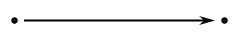
\includegraphics[width=0.8\linewidth]{figures/intro/scg/arcs/const/scg_const_perm_positive2.png}} & \parbox[|c]{2cm}{\centering\ni} & \parbox[|m]{2cm}{\centering\in} & \parbox[|c]{2cm}{\centering->} & \parbox[|m|]{2cm}{\centering<-} \\
	\hline
	
	\parbox[m|]{4.6cm}{\textit{\\ константная постоянная негативная sc-дуга принадлежности \\}} & \parbox[m|]{3.5cm}{\centering 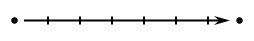
\includegraphics[width=0.8\linewidth]{figures/intro/scg/arcs/const/scg_const_perm_negative2.png}} & \parbox[m]{2cm}{\centering \not\ni} & \parbox[m|]{2cm}{\centering\notin} & \parbox[m|]{2cm}{\centering-|>} & \parbox[m]{2cm}{\centering<|-} \\
	\hline
	
	\parbox[m]{4.6cm}{\textit{\\ константная постоянная нечеткая sc-дуга принадлежности \\}} & \parbox[m]{3.5cm}{\centering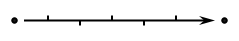
\includegraphics[width=0.8\linewidth]{figures/intro/scg/arcs/const/scg_const_perm_fuzzy2.png}} & \parbox[m]{2cm}{\centering / \ni} & \parbox[m]{2cm}{\centering \in /} & \parbox[m]{2cm}{\centering -/>} & \parbox[m]{2cm}{\centering </-} \\
	\hline
	
	\parbox[m]{4.6cm}{\textit{\\ константная временная позитивная sc-дуга принадлежности \\}} & \parbox[m]{3.5cm}{\centering 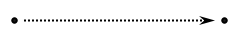
\includegraphics[width=0.8\linewidth]{figures/intro/scg/arcs/const/scg_const_temp_positive2.png}} & \parbox[m]{2cm}{\centering \sim \ni} & \parbox[m]{2cm}{\centering \in \sim} & \parbox[m]{2cm}{\centering \sim>} & \parbox[m]{2cm}{\centering <\sim} \\
	\hline
	
	\parbox[m]{4.6cm}{\textit{\\ константная временная негативная sc-дуга принадлежности \\}} & \parbox[m]{3.5cm}{\centering 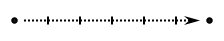
\includegraphics[width=0.8\linewidth]{figures/intro/scg/arcs/const/scg_const_temp_negative2.png}} & \parbox[m]{2cm}{\centering \sim \not\ni} & \parbox[m]{2cm}{\centering \notin \sim} & \parbox[m]{2cm}{\centering \sim|>} & \parbox[m]{2cm}{\centering <|\sim} \\
	\hline
	
	\parbox[m]{4.6cm}{\textit{\\ константная временная нечеткая sc-дуга принадлежности \\}} & \parbox[m]{3.5cm}{\centering 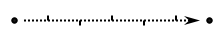
\includegraphics[width=0.8\linewidth]{figures/intro/scg/arcs/const/scg_const_temp_fuzzy2.png}} & \parbox[m]{2cm}{\centering \sim / \ni}  & \parbox[m]{2cm}{\centering \in/\sim} & \parbox[m]{2cm}{\centering \sim/>} & \parbox[m]{2cm}{\centering </\sim} \\
	\hline
	
	\parbox[m]{4.6cm}{\textit{\\ переменная постоянная позитивная sc-дуга принадлежности \\}} & \parbox[m]{3.5cm}{\centering 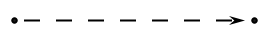
\includegraphics[width=0.8\linewidth]{figures/intro/scg/arcs/var/scg_var_perm_positive2.png}} & \parbox[m]{2cm}{\centering \textunderscore \ni} & \parbox[m]{2cm}{\centering \textunderscore \in} & \parbox[m]{2cm}{\centering \textunderscore->} & \parbox[m]{2cm}{\centering <-\textunderscore} \\
	\hline
	
	\parbox[m]{4.6cm}{\textit{\\ переменная постоянная негативная sc-дуга принадлежности \\}} & \parbox[m]{3.5cm}{\centering 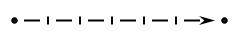
\includegraphics[width=0.8\linewidth]{figures/intro/scg/arcs/var/scg_var_perm_negative2.png}} & \parbox[m]{2cm}{\centering \textunderscore \not\ni} & \parbox[m]{2cm}{\centering \notin \textunderscore} & \parbox[m]{2cm}{\centering \textunderscore-|>} & \parbox[m]{2cm}{\centering <|-\textunderscore} \\
	\hline
	
	\parbox[m]{4.6cm}{\textit{\\ переменная постоянная нечеткая sc-дуга принадлежности \\}} & \parbox[m]{3.5cm}{\centering 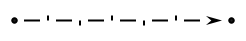
\includegraphics[width=0.8\linewidth]{figures/intro/scg/arcs/var/scg_var_perm_fuzzy2.png}} & \parbox[m]{2cm}{\centering \textunderscore /\ni} & \parbox[m]{2cm}{\centering \in/\textunderscore} & \parbox[m]{2cm}{\centering \textunderscore-/>} & \parbox[m]{2cm}{\centering </-\textunderscore} \\
	\hline
	
	\parbox[m]{4.6cm}{\textit{\\ переменная временная позитивная sc-дуга принадлежности \\}} & \parbox[m]{3.5cm}{\centering 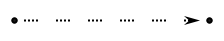
\includegraphics[width=0.8\linewidth]{figures/intro/scg/arcs/var/scg_var_temp_positive2.png}} & \parbox[m]{2cm}{\centering \textunderscore \sim \ni} & \parbox[m]{2cm}{\centering \in \sim \textunderscore} & \parbox[m]{2cm}{\centering \textunderscore \sim >} & \parbox[m]{2cm}{\centering < \sim \textunderscore} \\
	\hline
	
	\parbox[m]{4.6cm}{\textit{\\ переменная временная негативная sc-дуга принадлежности \\}} & \parbox[m]{3.5cm}{\centering 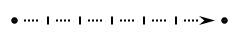
\includegraphics[width=0.8\linewidth]{figures/intro/scg/arcs/var/scg_var_temp_negative2.png}} & \parbox[m]{2cm}{\centering \textunderscore \sim \not$\ni$} & \parbox[c]{2cm}{\centering \notin \sim \textunderscore} & \parbox[m]{2cm}{\centering \textunderscore \sim |>} & \parbox[m]{2cm}{\centering <| \sim \textunderscore} \\
	\hline
	
	\parbox[m]{4.6cm}{\textit{\\переменная временная нечеткая sc-дуга принадлежности\\}} & \parbox[m]{3.5cm}{\centering 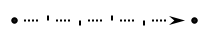
\includegraphics[width=0.8\linewidth]{figures/intro/scg/arcs/var/scg_var_temp_fuzzy2.png}} & \parbox[m]{2cm}{\centering \textunderscore \sim / \ni} & \parbox[m]{2cm}{\centering \in/\sim\textunderscore} & \parbox[m]{2cm}{\centering \textunderscore \sim />} & \parbox[m]{2cm}{\centering </\sim \textunderscore} \\
	\hline
	
	\parbox[m]{4.6cm}{\textit{\\метапеременная постоянная позитивная sc-дуга принадлежности\\}} & \parbox[m]{3.5cm}{\centering 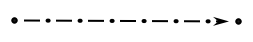
\includegraphics[width=0.8\linewidth]{figures/intro/scg/arcs/meta/scg_metavar_perm_positive2.png}} & \parbox[m]{2cm}{\centering\textunderscore \textunderscore\ni} & \parbox[m]{2cm}{\centering\in\textunderscore\textunderscore} & \parbox[m]{2cm}{\centering\textunderscore\textunderscore->} & \parbox[m]{2cm}{\centering <-\textunderscore\textunderscore} \\
	\hline
	
	\parbox[m]{4.6cm}{\textit{\\ метапеременная постоянная негативная sc-дуга принадлежности \\}} & \parbox[m]{3.5cm}{\centering 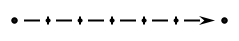
\includegraphics[width=0.8\linewidth]{figures/intro/scg/arcs/meta/scg_metavar_perm_negative2.png}} & \parbox[m]{2cm}{\centering \textunderscore\textunderscore \not\ni} & \parbox[m]{2cm}{\centering \notin\textunderscore\textunderscore} & \parbox[m]{2cm}{\centering \textunderscore\textunderscore-|>} & \parbox[m]{2cm}{\centering <|-\textunderscore\textunderscore} \\
	\hline
	
	\parbox[m]{4.6cm}{\textit{\\ метапеременная постоянная нечеткая sc-дуга принадлежности \\}} & \parbox[m]{3.5cm}{\centering 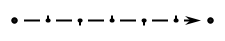
\includegraphics[width=0.8\linewidth]{figures/intro/scg/arcs/meta/scg_metavar_perm_fuzzy2.png}} & \parbox[m]{2cm}{\centering\textunderscore\textunderscore/\ni} & \parbox[m]{2cm}{\centering\in/\textunderscore\textunderscore} & \parbox[m]{2cm}{\centering\textunderscore\textunderscore-/>} & \parbox[m]{2cm}{\centering </-\textunderscore\textunderscore} \\
	\hline
	
	\parbox[m]{4.6cm}{\textit{\\ метапеременная временная позитивная sc-дуга принадлежности \\}} & \parbox[m]{3.5cm}{\centering 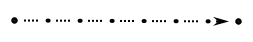
\includegraphics[width=0.8\linewidth]{figures/intro/scg/arcs/meta/scg_metavar_temp_positive2.png}} & \parbox[m]{2cm}{\centering\textunderscore\textunderscore\sim\ni} & \parbox[m]{2cm}{\centering\in\sim\textunderscore\textunderscore} & \parbox[m]{2cm}{\centering\textunderscore\textunderscore\sim>} & \parbox[m]{2cm}{\centering <\sim\textunderscore\textunderscore} \\
	\hline
	
	\parbox[m]{4.6cm}{\textit{\\ метапеременная временная негативная sc-дуга принадлежности \\}} & \parbox[m]{3.5cm}{\centering 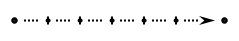
\includegraphics[width=0.8\linewidth]{figures/intro/scg/arcs/meta/scg_metavar_temp_negative2.png}} & \parbox[m]{2cm}{\centering \textunderscore\textunderscore\sim \not\ni} & \parbox[m]{2cm}{\centering\notin\sim\textunderscore\textunderscore} & \parbox[m]{2cm}{\centering\textunderscore\textunderscore\sim|>} & \parbox[m]{2cm}{\centering <|\sim\textunderscore\textunderscore} \\
	\hline
	
	\parbox[m]{4.6cm}{\textit{\\ метапеременная временная нечеткая sc-дуга принадлежности \\}} & \parbox[m]{3.5cm}{\centering 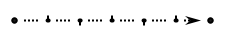
\includegraphics[width=0.8\linewidth]{figures/intro/scg/arcs/meta/scg_metavar_temp_fuzzy2.png}} & \parbox[m]{2cm}{\centering \textunderscore\textunderscore\sim/\ni} & \parbox[m]{2cm}{\centering\in/\sim\textunderscore\textunderscore} & \parbox[m]{2cm}{\centering\textunderscore\textunderscore\sim/>} & \parbox[m]{2cm}{\centering</\sim\textunderscore\textunderscore} \\
	\hline
\end{longtable}
}
%---------------------------------------------
\scnheader{Таблица. Алфавит sc.s-коннекторов, соответствующих sc.g-коннекторам, которые не являются sc.g-дугами принадлежности}
\scneqtable{
\begin{longtable}[l]{|m{6.2cm}|m{2.5cm}|m{2.5cm}|m{2.5cm}|m{2.5cm}|}
	\hline
	\multicolumn{1}{|c}{\parbox[c]{6.2cm}{Изображение \textit{sc-коннектора} в SCg}} &
	\multicolumn{2}{|c}{\parbox[c]{5cm}{Изображение \textit{sc.s-коннектора} в Расширенном алфавите}} &
	\multicolumn{2}{|c|}{\parbox[c]{5cm}{Изображение \textit{sc.s-коннектора} в Базовом алфавите}}
	\hline
	\endhead
	
	\parbox[|c]{6.2cm}{\\\centering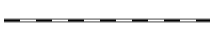
\includegraphics[width=0.8\linewidth]{figures/intro/scs/sc.s-connectors/noorient.png}\\} & \multicolumn{2}{c|}{ \parbox[c]{5cm}{\centering\leftrightarrow}} & \multicolumn{2}{c|}{ \parbox[c]{5cm}{\centering<>}} \\
	\hline
	
	\parbox[c]{6.2cm}{\\\centering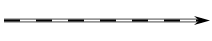
\includegraphics[width=0.8\linewidth]{figures/intro/scs/sc.s-connectors/orient.png} \\} &\parbox[c]{2.5cm}{\\\centering\rightarrow\\} & \parbox[c]{2.5cm}{\\\centering\leftarrow\\} & \parbox[c]{2.5cm}{\\\centering >>\\} & \parbox[c|]{2.5cm}{\\\centering <<\\} \\
	\hline
	
	\parbox[c]{6.2cm}{\\\centering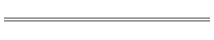
\includegraphics[width=0.8\linewidth]{figures/intro/scs/sc.s-connectors/constPermNoorien.png}\\} & \multicolumn{2}{c|}{\parbox[c]{5cm}{\centering\Leftrightarrow}} & \multicolumn{2}{c|}{\parbox[c]{5cm}{\centering<=>}} \\
	\hline
	
	\parbox[c]{6.2cm}{\\\centering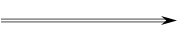
\includegraphics[width=0.8\linewidth]{figures/intro/scs/sc.s-connectors/constPermOrient.png}\\} & \parbox[c]{2.5cm}{\centering\Rightarrow} & \parbox[c]{2.5cm}{\centering\Leftarrow} & \parbox[c]{2.5cm}{\centering =>} & \parbox[c|]{2.5cm}{\centering <=} \\
	\hline
	
	\parbox[c]{6.2cm}{\\\centering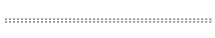
\includegraphics[width=0.8\linewidth]{figures/intro/scs/sc.s-connectors/constTempNoorien.png}\\} & \multicolumn{2}{c|}{\parbox[c]{5cm}{\centering\sim\Leftrightarrow}} & \multicolumn{2}{c|}{\parbox[c|]{5cm}{\centering\sim<=>}} \\
	\hline
	
	\parbox[c]{6.2cm}{\\\centering 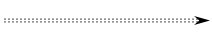
\includegraphics[width=0.8\linewidth]{figures/intro/scs/sc.s-connectors/constTempOrient.png}\\} & \parbox[c]{2.5cm}{\centering\sim\Rightarrow} & \parbox[c]{2.5cm}{\centering\Leftarrow\sim} & \parbox[c]{2.5cm}{\centering\sim=>} & \parbox[c|]{2.5cm}{\centering <=\sim} \\
	\hline
	
	\parbox[c]{6.2cm}{\\\centering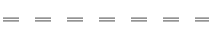
\includegraphics[width=0.8\linewidth]{figures/intro/scs/sc.s-connectors/varPermNoorien.png}\\} & \multicolumn{2}{c|}{\parbox[c]{5cm}{\centering\textunderscore\Leftrightarrow}} & \multicolumn{2}{c|}{\parbox[c|]{5cm}{\centering\textunderscore<=>}} \\
	\hline
	
	\parbox[c]{6.2cm}{\\\centering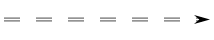
\includegraphics[width=0.8\linewidth]{figures/intro/scs/sc.s-connectors/varPermOrient.png}\\} & \parbox[c]{2.5cm}{\centering\textunderscore\Rightarrow} & \parbox[c]{2.5cm}{\centering\Leftarrow\textunderscore} & \parbox[c]{2.5cm}{\centering\textunderscore=>} & \parbox[c|]{2.5cm}{\centering <=\textunderscore} \\
	\hline
	
	\parbox[c]{6.2cm}{\\\centering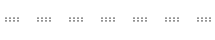
\includegraphics[width=0.8\linewidth]{figures/intro/scs/sc.s-connectors/varTempNoorien.png}\\} & \multicolumn{2}{c|}{\parbox[c]{5cm}{\centering\textunderscore\sim\Leftrightarrow}} & \multicolumn{2}{c|}{\parbox[c]{5cm}{\centering\textunderscore\sim<=>}} \\
	\hline
	
	\parbox[c]{6.2cm}{\\\centering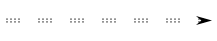
\includegraphics[width=0.8\linewidth]{figures/intro/scs/sc.s-connectors/varTempOrient.png}\\} & \parbox[c]{2.5cm}{\centering\textunderscore\sim\Rightarrow} & \parbox[c]{2.5cm}{\centering\Leftarrow\sim\textunderscore} & \parbox[c]{2.5cm}{\centering\textunderscore\sim=>} & \parbox[c|]{2.5cm}{\centering <=\sim\textunderscore} \\
	\hline
	
	\parbox[c]{6.2cm}{\\\centering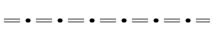
\includegraphics[width=0.8\linewidth]{figures/intro/scs/sc.s-connectors/metaPermNoorien.png}\\} & \multicolumn{2}{c|}{\parbox[c]{5cm}{\centering\textunderscore\textunderscore\Leftrightarrow}} & \multicolumn{2}{c|}{\parbox[c|]{5cm}{\centering\textunderscore\textunderscore<=>}} \\
	\hline
	
	\parbox[c]{6.2cm}{\\\centering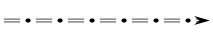
\includegraphics[width=0.8\linewidth]{figures/intro/scs/sc.s-connectors/metaPermOrient.png}\\} & \parbox[c]{2.5cm}{\centering\textunderscore\textunderscore\Rightarrow} & \parbox[c]{2.5cm}{\centering\Leftarrow\textunderscore\textunderscore} & \parbox[c]{2.5cm}{\centering\textunderscore\textunderscore=>} & \parbox[c|]{2.5cm}{\centering <=\textunderscore\textunderscore} \\
	\hline
	
	\parbox[c]{6.2cm}{\\\centering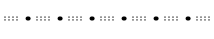
\includegraphics[width=0.8\linewidth]{figures/intro/scs/sc.s-connectors/metaTempNoorien.png}\\} & \multicolumn{2}{c|}{\parbox[c]{5cm}{\centering\textunderscore\textunderscore\sim\Leftrightarrow}} & \multicolumn{2}{c|}{\parbox[c]{5cm}{\centering\textunderscore\textunderscore\sim<=>}} \\
	\hline
	
	\parbox[c]{6.2cm}{\\\centering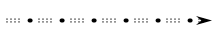
\includegraphics[width=0.8\linewidth]{figures/intro/scs/sc.s-connectors/metaTempOrient.png}\\} & \parbox[c]{2.5cm}{\centering\textunderscore\textunderscore\sim\Rightarrow} & \parbox[c]{2.5cm}{\centering\Leftarrow\sim\textunderscore\textunderscore} & \parbox[c]{2.5cm}{\centering\textunderscore\textunderscore\sim\Rightarrow} & \parbox[c|]{2.5cm}{\centering\Leftarrow\sim\textunderscore\textunderscore} \\
	\hline
	
	\parbox[c]{6.2cm}{\\\centering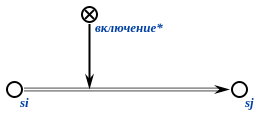
\includegraphics[width=0.8\linewidth]{figures/intro/scs/sc.s-connectors/examples/scs_transf_inclusion_const.png}\\} & \parbox[c]{2.5cm}{\centering\supseteq} & \parbox[c]{2.5cm}{\centering\subseteq} & \multicolumn{2}{c|}{\parbox[c]{5cm}{}} \\
	\hline
	
	\parbox[c]{6.2cm}{\\\centering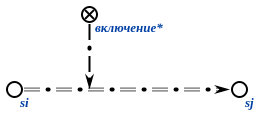
\includegraphics[width=0.8\linewidth]{figures/intro/scs/sc.s-connectors/examples/scs_transf_inclusion_meta.png}\\} & \parbox[c]{2.5cm}{\centering\textunderscore\supseteq} & \parbox[c]{2.5cm}{\centering\subseteq\textunderscore} & \multicolumn{2}{c|}{\parbox[c|]{5cm}{\centering}} \\
	\hline
	
	\parbox[c]{6.2cm}{\\\centering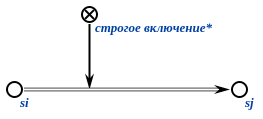
\includegraphics[width=0.8\linewidth]{figures/intro/scs/sc.s-connectors/examples/scs_transf_strict_inclusion_const.png}\\} & \parbox[c]{2.5cm}{\centering\supset} & \parbox[c]{2.5cm}{\centering\subset} & \multicolumn{2}{c|}{\parbox[c|]{5cm}{}} \\
	\hline
	
	\parbox[c]{6.2cm}{\\\centering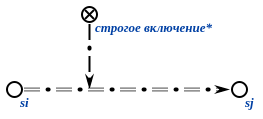
\includegraphics[width=0.8\linewidth]{figures/intro/scs/sc.s-connectors/examples/scs_transf_strict_inclusion_meta.png}\\} & \parbox[c]{2.5cm}{\centering\textunderscore\supset} & \parbox[c]{2.5cm}{\centering\subset\textunderscore} & \multicolumn{2}{c|}{\parbox[c|]{5cm}{}} \\
	\hline
	
	\parbox[c]{6.2cm}{\\\centering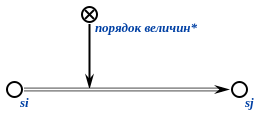
\includegraphics[width=0.8\linewidth]{figures/intro/scs/sc.s-connectors/examples/scs_transf_value_order_const.png}\\} & \parbox[c]{2.5cm}{\centering\geq} & \parbox[c]{2.5cm}{\centering\leq} & \multicolumn{2}{c|}{\parbox[c|]{5cm}{}} \\
	\hline
	
	\parbox[c]{6.2cm}{\\\centering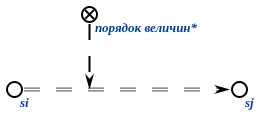
\includegraphics[width=0.8\linewidth]{figures/intro/scs/sc.s-connectors/examples/scs_transf_value_order_var.png}\\} & \parbox[c]{2.5cm}{\centering\textunderscore\geq} & \parbox[c]{2.5cm}{\centering\textunderscore\leq} & \multicolumn{2}{c|}{\parbox[c]{5cm}{}}  \\
	\hline
	
	\parbox[c]{6.2cm}{\\\centering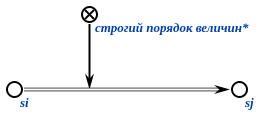
\includegraphics[width=0.8\linewidth]{figures/intro/scs/sc.s-connectors/examples/scs_transf_value_strict_order_const.png}\\} & \parbox[c]{2.5cm}{\centering >} & \parbox[c]{2.5cm}{\centering <} & \multicolumn{2}{c|}{\parbox[c]{5cm}{}} \\
	\hline
	
	\parbox[c]{6.2cm}{\\\centering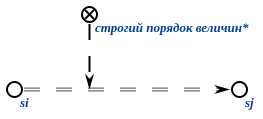
\includegraphics[width=0.8\linewidth]{figures/intro/scs/sc.s-connectors/examples/scs_transf_value_strict_order_var.png}\\} & \parbox[c]{2.5cm}{\centering\textunderscore>} & \parbox[c]{2.5cm}{\centering <\textunderscore} & \multicolumn{2}{c|}{\parbox[c]{5cm}{}} \\
	\hline
	
	\parbox[c]{6.2cm}{\\\centering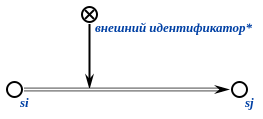
\includegraphics[width=0.8\linewidth]{figures/intro/scs/sc.s-connectors/examples/scs_transf_external_idtf_const.png}\\} & \multicolumn{2}{c|}{\parbox[c]{5cm}{\centering :=}} & \multicolumn{2}{c|}{\parbox[c]{5cm}{}} \\
	\hline
	
	\parbox[c]{6.2cm}{\\\centering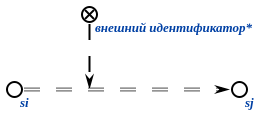
\includegraphics[width=0.8\linewidth]{figures/intro/scs/sc.s-connectors/examples/scs_transf_external_idtf_var.png}\\} & \multicolumn{2}{c|}{\parbox[c]{5cm}{\centering\textunderscore:=}} & \multicolumn{2}{c|}{\parbox[c]{5cm}{}} \\
	\hline
	
	\parbox[c]{6.2cm}{\\\centering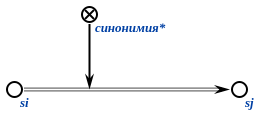
\includegraphics[width=0.8\linewidth]{figures/intro/scs/sc.s-connectors/examples/scs_transf_synonymy_const.png}\\} & \multicolumn{2}{c|}{\parbox[c]{5cm}{\centering =}} & \multicolumn{2}{c|}{\parbox[c]{5cm}{}} \\
	\hline
	
	\parbox[c]{6.2cm}{\\\centering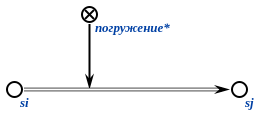
\includegraphics[width=0.8\linewidth]{figures/intro/scs/sc.s-connectors/examples/scs_transf_insertion_const.png}\\} & \parbox[c]{2.5cm}{\centering\supset=} & \parbox[c]{2.5cm}{\centering = \subset} &  \multicolumn{2}{c|}{\parbox[c]{5cm}{}}  \\
	\hline
\end{longtable}
}

\scnendstruct \scninlinesourcecommentpar{Завершили Описание sc.s-разделителей и sc.s-ограничителей}

\scnsegmentheader{Описание sc.s-предложений}
\scnstartsubstruct

\scnheader{sc.s-предложение}
\scnidtf{минимальный семантически целостный фрагмент sc.s-текста}
\scnidtf{минимальный sc.s-текст}
\scnsubset{sc.s-текст}
\scnsuperset{простое sc.s-предложение\\
    \scnaddlevel{1}
    \scnidtf{минимальное sc.s-предложение}
    \scnexplanation{\textit{sc.s-предложение}, (1) \uline{состоящее} или из двух \textit{sc-идентификаторов}, соединенных между собой \textit{sc.s-коннектором}, или из трех \textit{sc-идентификаторов}, разделенных \textit{sc.s-разделителями, изображающими связь инцидентности sc-элементов}, и (2) завершающееся \textit{двойной точкой с запятой}}
    \scnnote{Нетрудно заметить, что простые sc.s-предложения по сути аналогичны триплетам языка RDF (RDF-триплетам), за тем исключением, что \textit{простое sc.s-предложение} можно "развернуть"\ при помощи \textit{Операции конверсии sc.s-предложений*} не меняя при этом его смысл, а RDF-триплет нельзя. Это является одной из причин, по которой, в отличие от RDF-триплетов, в простых sc.s-предложениях \textit{sc.s-коннекторы} и \textit{sc.s-разделители, изображающие связь инцидентности sc-элементов} не могут быть опущены, поскольку они в том числе показывают направление изображаемой ими связи между sc-элементами.}
\scnrelfromlist{пример}{
    \scnfileitem{\textit{многоугольник} $\supset$ \textit{треугольник}}
    \scnaddlevel{1}
    \scnrelboth{семантическая эквивалентность}{\scnfilescg{figures/intro/scs/inclusion.png}}
    \scnaddlevel{-1};
    \scnfileitem{\textit{сторона*} $\ni$ (\textit{Четырехугк(ТчкА\char59ТчкВ\char59ТчкС\char59ТчкD)} $\Rightarrow$ \textit{Отр(ТчкВ\char59ТчкС)})\char59\char59}
    \scnaddlevel{1}
    \scnrelboth{семантическая эквивалентность}{\scnfilescg{figures/intro/scs/side.png}}
    \scnaddlevel{-1};
    \scnfileitem{\textit{Si} |- \textit{ai} >| \textit{ei}}
    \scnaddlevel{1}
    \scnrelboth{семантическая эквивалентность}{\scnfilescg{figures/intro/scs/inclusion_incident.png}}
    \scnaddlevel{-1}
    }
\scnaddlevel{-1}}
\scnnote{Признаком завершения любого \textit{sc.s-предложения}, т.е. последними его символами является \textit{двойная точка с запятой}, которую, следовательно, можно считать разделителем \textit{sc.s-предложений}.}
\scnrelfromlist{заданная операция}{Операция конверсии sc.s-предложения*\\
    \scnaddlevel{1}
    \scnsubset{синтаксическая трансформация*}
    \scnexplanation{Каждое \textit{sc.s-предложение} (в том числе, и \textit{простое sc.s-предложение}) можно преобразовать в семантически эквивалентное ему \textit{sc.s-предложение} путем конверсии ("разворота") цепочки компонентов \textit{sc.s-предложения}. Так, например, при конверсии ("развороте") простого \textit{sc.s-предложения} (1) первый его \textit{sc-идентификатор} (первый компонент этого \textit{sc.s-предложения}) становится третьим компонентом конвертированного\textit{ sc.s-предложения}, (2) второй его \textit{sc-идентификатор} (третий компонент исходного \textit{sc.s-предложения}) становится первым компонентом "конвертированного"\ \textit{sc.s-предложения} и (3) второй компонент исходного \textit{sc.s-предложения} (\textit{sc.s-коннектор} или \textit{sc.s-разделитель, изображающий связь инцидентности sc-элементов}, соединяющий указанные выше компоненты) остается вторым компонентом конвертированного \textit{sc.s-предложения}, но меняет направленность ("$\ni$"\ заменяется на "$\in$"\ и наоборот, "$\supset$"\ на "$\subset$"\ и наоборот, "$\Rightarrow$"\ на "$\Leftarrow$"\ и наоборот и т.д.)}
    \scnnote{Можно говорить не только о конверсии sc.s-предложения, но и о конверсии sc.s-коннектора, о конверсии sc.s-разделителя, изображающего связь инцидентности sc.s-элементов.}
    \scnrelfrom{sc.s-текст до трансформации}{\scnfilelong{\textit{треугольник $\ni$ Треуг(ТчкВ\char59ТчкС\char59ТчкD)}\char59\char59}}
    \scnrelfrom{sc.s-текст после трансформации}{\scnfilelong{\textit{Треуг(ТчкВ\char59ТчкС\char59ТчкD) $\in$ треугольник}\char59\char59}}
	\scnaddlevel{1}
    \scnrelboth{семантическая эквивалентность}{\scnfilescg{figures/intro/scs/conversion.png}}
    \scnaddlevel{-2}
;Операция присоединения sc.s-предложения*\\
    \scnaddlevel{1}
    \scnsubset{синтаксическая трансформация*}
    \scnidtf{Операция соединения двух sc.s-предложений при совпадении последнего компонента первого предложения с первым компонентом второго*}
    \scnexplanation{В результате выполнения данной операции:
    \begin{scnitemize}
        \item первый компонент второго sc.s-предложения удаляется\char59
        \item оставшаяся часть второго предложения окружается sc.s-ограничителем присоединенных предложений ("(*"\ и "*)"). Разделитель sc.s-предложений (";;") также попадает внутрь указанного ограничителя\char59
        \item полученная конструкция помещается между последним компонентом первого предложения и разделителем sc.s-предложений, которым заканчивалось первое предложение\char59
        \item второе предложение, таким образом, становится присоединенным sc.s-предложением.
    \end{scnitemize}
    Аналогичным образом к любому присоединенному sc.s-предложению могут "пристыковываться"\ другие присоединенные sc.s-предложения, в общем случае уровень такой вложенности не ограничен.
    }
    \scnaddlevel{-1}
;Операция слияния sc.s-предложений*\\
    \scnaddlevel{1}
    \scnsubset{синтаксическая трансформация*}
    \scnidtf{Операция присоединения простого sc.s-предложения к sc.s-предложению, у которого последний sc.s-коннектор совпадает с sc.s-коннектором простого sc.s-предложения, а предшествующий указанному sc.s-коннектору sc-идентификатор совпадает с первым sc-идентификатором простого sc.s-предложения*}
    \scnexplanation{В результате выполнения этой операции совпадающие sc-идентификаторы и sc.s-коннекторы соединяемых sc.s-предложений "склеиваются"\ , а последние sc-иден\-ти\-фи\-ка\-то\-ры соединяемых \textit{sc.s-предложений} становятся последними компонентами объединенного \textit{sc.s-предложения},
    разделенными \textit{точкой с запятой}. Аналогичным образом можно присоединять сколько угодно простых \textit{sc.s-предложений}.}
    \scnaddlevel{-1}
;Операция разложения sc.s-предложений на простые sc.s-предложения*\\
    \scnaddlevel{1}
    \scnsubset{синтаксическая трансформация*}
    \scnexplanation{Каждое \textit{sc.s-предложение} можно разложить на множество \textit{простых sc.s-предложений}, т.е. представить в виде последовательности \textit{простых sc.s-предложений}.}
    \scnaddlevel{-1}
;Операция разложения sc.s-предложений на простые sc.s-предложения с sc.s-разделителем, изображающим связь инцидентности sc-элементов*\\
    \scnaddlevel{1}
    \scnsubset{синтаксическая трансформация*}
    \scnexplanation{Каждое \textit{sc.s-предложение} (в том числе и \textit{простое sc.s-предложение} с \textit{sc.s-коннектором}) можно представить в виде семантически эквивалентной последовательности \textit{простых sc.s-предложений} с \textit{sc.s-разделителем, изображающим связь инцидентности sc-элементов}.}
    \scnnote{Данная операция осуществляет \uline{однозначное} (!) формирование множества \textit{простых sc.s-предложений} указанного вида.}
    \scnaddlevel{-1}
    }

\scnheader{sc.s-предложение}
\scnnote{Операции, заданные на множестве \textit{sc.s-предложений} можно разделить на три группы:
    \begin{scnitemize}
        \item группа операций конверсии \textit{sc.s-предложений}, состоящая из одной операции;
        \item группа операций соединения \textit{sc.s-предложений};
        \item группа операций декомпозиции \textit{sc.s-предложений} и, в частности, операций разложения \textit{sc.s-предложений}.
    \end{scnitemize}
Очевидно, что операции соединения \textit{sc.s-предложений} и операции декомпозиции \textit{sc.s-предложений} являются обратными друг другу операциями.}
\scnaddlevel{-1}

\scnheader{Описание примеров выполнения операций, заданных на множестве sc.s-предложений}
\scnstartsubstruct

\bigskip

\scnfilelong{\textit{треугольник $\ni$ Треугк(ТчкВ\char59ТчкС\char59ТчкD)}\char59\char59}
\scnrelfrom{Операция конверсии sc.s-предложения}{\scnfilelong{\textit{Треугк(ТчкВ\char59ТчкС\char59ТчкD) $\in$ треугольник}\char59\char59}}
\scnaddlevel{1}
\scnrelboth{семантическая эквивалентность}{\scnfilescg{figures/intro/scs/conversion.png}}
\scnaddlevel{-1}

\bigskip\bigskip

{\scnfilelong{\textit{треугольник $\ni$ Треугк(ТчкВ\char59ТчкС\char59ТчкD)\char59\char59
\newline
Треугк(ТчкВ\char59ТчкС\char59ТчкD) $\Rightarrow$ сторона*:включение*: Отр(ТчкВ\char59ТчкC)\char59\char59}}}
\scnrelfrom{Операция присоединения sc.s-предложения}{\scnfilelong{\textit{треугольник $\ni$ Треугк(ТчкВ\char59ТчкС\char59ТчкD) (* $\Rightarrow$ сторона*:включение*:Отр(ТчкВ\char59ТчкС)\char59\char59*) }\char59\char59}}
\scnaddlevel{1}
\scnrelboth{семантическая эквивалентность}{\scnfilescg{figures/intro/scs/joining_sentences.png}}
\scnaddlevel{-1}

\bigskip\bigskip

\scnfilelong{\textit{сторона* $\ni$ (Треугк(ТчкВ\char59Тчк С\char59ТчкD) $\Rightarrow$ Отр(ТчкВ\char59ТчкС))\char59\char59
\newline
сторона* $\ni$ (Треугк(ТчкВ\char59Тчк С\char59ТчкD) $\Rightarrow$ Отр(ТчкC\char59ТчкD))\char59\char59}}
\scnrelfrom{Операция слияния sc.s-предложений}{\scnfilelong{\textit{сторона* $\ni$ ((Треугк(ТчкВ\char59ТчкС\char59ТчкD) $\Rightarrow$ Отр(ТчкВ\char59ТчкС))\char59(Треуг(ТчкВ\char59ТчкС\char59ТчкD) $\Rightarrow$ Отр(ТчкC\char59ТчкD)))\char59\char59}}}
\scnaddlevel{1}
\scnrelfrom{синтаксическая трансформация}{\scnfilelong{\textit{Треугк(ТчкВ\char59ТчкС\char59ТчкD)}$\Rightarrow$\textit{сторона*}: \textit{Отр(ТчкВ\char59ТчкС)}\char59\textit{Отр(ТчкС\char59ТчкD)}\char59\char59}}
\scnrelboth{семантическая эквивалентность}{\scnfilescg{figures/intro/scs/joining_sentence.png}}
\scnaddlevel{-1}

\bigskip\bigskip

{\scnfilelong{\textit{Треугк(ТчкВ\char59ТчкС\char59ТчкD) $\Rightarrow$ сторона*:включение*:Отр(ТчкВ\char59ТчкС)\char59\char59}}}
\scnrelfrom{Операция разложения sc.s-предложений на простые sc.s-предложения}{\scnfilelong{\textit{сторона* $\ni$ (Треугк(ТчкВ\char59ТчкС\char59ТчкD) $\Rightarrow$ Отр(ТчкВ\char59ТчкС))\char59\char59
\newline включение* $\ni$ (Треугк(ТчкВ\char59ТчкС\char59ТчкD) $\Rightarrow$ Отр(ТчкВ\char59ТчкС))\char59\char59}}}
\scnaddlevel{1}
\scnrelboth{семантическая эквивалентность}{\scnfilescg{figures/intro/scs/dividing_sentences.png}}
\scnaddlevel{-1}

\bigskip\bigskip

{\scnfilelong{\textit{треугольник $\ni$ Треугк(ТчкВ\char59ТчкC\char59ТчкD)}}}
\scnrelfrom{Операция разложения sc.s-предложений на простые sc.s-предложения с sc.s-разделителем, изображающим связь инцидентности sc-элементов}{\scnfilelong{\textit{треугольник |- ai >| Треугк(ТчкВ\char59ТчкС\char59ТчкD)\char59\char59
\newline
константный постоянный sc-узел, обозначающий класс $\ni$ треугольник\char59\char59
\newline
константная постоянная позитивная sc-дуга принадлежности $\ni$ ai\char59\char59
\newline
константный постоянный sc-узел общего вида $\ni$ Треугк(ТчкВ\char59ТчкC\char59ТчкD)\char59\char59}}}
\scnaddlevel{1}
\scnrelboth{семантическая эквивалентность}{\scnfilescg{figures/intro/scs/dividing_sentences_incident.png}}
\scnaddlevel{-1}

\scnendstruct

\scnheader{присоединенное sc.s-предложение}
\scnidtf{встроенное sc.s-предложение}
\scnexplanation{Присоединенные sc.s-предложения используются для того, чтобы продолжить спецификацию какого-либо sc-элемента, sc-идентификатор которого является последним компонентом в рамках какого-либо sc.s-предложения, не начиная при этом нового sc.s-предложения и, таким образом, не дублируя указанный sc-идентификатор. Внутрь присоединенных sc.s-предложений также могут встраиваться другие присоединенные sc.s-предложения, в общем случае уровень вложенности таких предложений не ограничен. Таким образом присоединенные sc.s-предложения описывают "ветвление"\ sc.s-предложений, при этом точками такого "ветвления"\ выступают sc-идентификаторы, входящие в состав этих sc.s-предложений.

Благодаря введению присоединенных sc.s-предложений появляется возможность любой sc-текст изобразить в виде одного sc.s-предложения, содержащего необходимое количество присоединенных sc.s-предложений. Таким образом, SCs-код по выразительной мощности становится эквивалентным SCn-коду.}

\scnheader{sc.s-предложение}
\scntext{денотационная семантика}{С семантической точки зрения \textit{sc.s-предложение} представляет собой описание некоторого \uline{маршрута} в соответствующем sc-тексте, который является графовой структурой специального вида и структура которого описывается (изображается) с помощью \textit{sc.s-предложений}. Указанный маршрут "проводится"\ по sc-коннекторам и по связям инцидентности sc-элементов, если маршрут проходит через инцидентные sc-коннекторы. В описании указанного маршрута могут дополнительно указываться множества (чаще всего отношения), которым принадлежат sc-коннекторы, входящие в описываемый маршрут. Кроме того, указанный маршрут в начале и/или в конце может иметь разветвления, когда какой-либо sc-элемент \uline{одинаково} инцидентен нескольким \uline{однотипным} sc-коннекторам, соединяющим указанный sc-элемент с некоторыми другими sc-элементами.

Таким образом каждое указанное разветвление состоит из неограниченного числа ветвей, каждая из которых состоит из одного sc-коннектора и одного связываемого им sc-элемента.}

\scnheader{компонент sc.s-предложения*}
\scnexplanation{Каждое \textit{sc.s-предложение} представляет собой последовательность (1) \textit{sc-идентификаторов}, (2) \textit{sc.s-коннекторов} или \textit{sc.s-разделителей}, изображающих связь инцидентности \textit{sc-элементов}, (3) \textit{точек с запятыми}, (4) \textit{ограничителей присоединенных sc.s-предложений}, завершаемая \textit{двойной точкой с запятой}. При этом непосредственно соседствовать друг с другом не могут ни \textit{sc-идентификаторы}, ни \textit{sc.s-коннекторы}, ни, очевидно, \textit{точки с запятыми} и \textit{ограничители присоединенных sc.s-предложений}.\\
Между \textit{sc-идентификаторами} в рамках \textit{sc.s-предложения} может находиться либо \textit{точка с запятой}, либо \textit{sc.s-коннектор}, либо \textit{sc.s-разделитель}, изображающий связь инцидентности \textit{sc-элементов}. Слева и справа от \textit{sc.s-коннектора} и от \textit{sc.s-разделителя}, изображающего связь инцидентности \textit{sc-элементов}, должны находиться \textit{sc-идентификаторы}.

Указанные \textit{sc-идентификаторы}, \textit{sc.s-коннекторы} и \textit{sc.s-разделители}, изображающие связь инцидентности \textit{sc-элементов}, считаются компонентами соответствующего \textit{sc.s-предложения}. Понятие "быть компонентом sc.s-предложения"\ является относительным понятием (отношением), т.к. в состав некоторых компонентов \textit{sc.s-предложения} (в состав \textit{sc-идентификаторов}, являющихся \textit{sc.s-выражениями}, ограничиваемыми фигурными или квадратными скобками) могут входить других \textit{sc.s-предложения}, состоящие из своих компонентов.}
\scnrelfrom{первый домен}{sc.s-предложение}
\scnrelfrom{второй домен}{{\normalfont (} sc-идентификатор $\cup$ sc.s-разделитель $\cup$ sc.s-ограничитель {\normalfont )}}

\scnheader{sc.s-модификатор*}
\scnsubset{компонент sc.s-предложения*}
\scnexplanation{Это дополнительный вид компонентов \textit{sc.s-предложений}. Каждый \textit{sc.s-модификатор}, являющийся компонентом некоторого \textit{sc.s-предложения}, представляет собой \textit{sc-идентификатор}, обозначающий множество (чаще всего, отношение), которому принадлежит sc-коннектор, изображенный \textit{sc.s-коннектором}, который предшествует указанному \textit{sc-идентификатору}. Признаком \textit{sc.s-модификатора} является \textit{двоеточие} (или \textit{двойное двоеточие}), которое ставится после \textit{sc.s-модификатора} и отделяет его либо от следующего за ним другого \textit{sc.s-модификатора} для этого же \textit{sc.s-коннектора}, либо от следующего за ним \textit{sc-идентификатора}, соответствующего sc-элементу, который инцидентен sc-коннектору, изображенному \textit{sc.s-коннектором}, находящимся левее рассматриваемого \textit{sc-идентификатора} после одного или нескольких \textit{sc.s-модификаторов}. Обычное ("одинарное") \textit{двоеточие} обозначает, что sc-элемент, изображенный соответствующим sc.s-модификатором, связан с sc-коннектором, изображенным левее этого sc.s-модификатора, \textit{базовой sc-дугой} (\textit{константной постоянной позитивной sc-дугой принадлежности}), \textit{двойное двоеточие} обозначает, что указанные элементы связаны \textit{переменной постоянной позитивной sc-дугой принадлежности}.}
\scnrelfromlist{пример}{
    \scnfileitem{\textit{Четырехугк(ТчкА;ТчкВ;ТчкС;ТчкD)} $\Rightarrow$ \textit{сторона*} : \textit{включение*} : \textit{Отр(ТчкВ;ТчкС)};; }\\
    \scnaddlevel{1}
    \scnrelboth{семантическая эквивалентность}{\scnfilescg{figures/intro/scs/modifier.png}}
    \scnaddlevel{-1};
    \scnfileitem{\textit{Треугк(ТчкА;ТчкВ;ТчкС)} $\_\Rightarrow$ \textit{сторона*} :: \textit{\_s};; }\\
    \scnaddlevel{1}
    \scnrelboth{семантическая эквивалентность}{\scnfilescg{figures/intro/scs/modifier_var.png}}
    \scnaddlevel{-1}
    }

\scnheader{sc.s-текст}
\scnidtf{конкатенация \textit{sc.s-предложений}}
\scnidtf{последовательность \textit{sc.s-предложений}, разделяемых \textit{двойными точками с запятой}}
\scnsuperset{максимальный исходный sc.s-текст}
    \scnaddlevel{1}
    \scnidtf{конкатенция \textit{sc.s-предложений}, слева и справа от которой отсутствуют какие-либо символы SCs-кода}
    \scnaddlevel{-1}
\scnsuperset{максимальный sc.s-текст, включенный в sc-структуру}
    \scnaddlevel{1}
    \scnidtf{конкатенция всех \textit{sc.s-предложений}, входящих в состав \textit{sc.s-выражения sc-структуры}}
    \scnsuperset{sc.s-текст, включенный в структуру}
        \scnaddlevel{1}
        \scnidtf{часть цепочки \textit{sc.s-предложений}, входящих в состав максимального sc.s-текста, включенного в sc-структуру}
        \scnsuperset{sc.s-предложение, включенное в sc-структуру}
    \scnaddlevel{-2}
\scnnote{\textit{sc.s-предложение} является минимальным sc.s-текстом.}
\scntext{свойство}{Смысл sc.s-текста (а также \textit{sc.s-текста, включенного в sc-структуру} не зависит от порядка \textit{sc.s-предложений} в этих sc-текстах. Т.е. перестановка \textit{sc.s-предложений} в рамках таких sc.s-текстов смысла этих sc.s-текстов не меняет (т.е. приводит к семантически эквивалентным sc.s-текстам), но сильно влияет на трудоемкость человеческого восприятия (на "читабельность") этих текстов.}
\scnrelfrom{пример}{\scnfilelong{
		\textit{материальный объект} $\ni$ \textit{Земля} (* => \textit{вращаться вокруг}*: \textit{спутник}*: \textit{Луна};;*);;\\
		\textit{материальный объект} $\ni$ \textit{Луна}(* => \textit{основной идентификатор}*: [Moon] (* <- \textit{Английский язык};; *); [Луна] (* <- \textit{Русский язык};; *);; *);;\\
		\textit{материальный объект} $\ni$ \textit{Солнце} (* => \textit{вращаться вокруг}*: \textit{Земля}; \textit{Марс};; *);;\\
		\textit{материальный объект} $\ni$ \textit{Марс};;}
}    
\scnaddlevel{1}
\scnrelfrom{семантическая эквивалентность}{ \scnfilescg{figures/intro/scs/scs_text_example.png}}
\scnaddlevel{-1}
    

\newpage

\scnauthorcomment{пересмотреть фрагмент}

\scnheader{sc.s-текст}
\scnidtf{конкатенация \textit{sc.s-предложений}}
\scnidtf{последовательность \textit{sc.s-предложений}, разделяемых \textit{двойными точками с запятой}}
\scnsuperset{максимальный исходный sc.s-текст}
    \scnaddlevel{1}
    \scnidtf{конкатенция \textit{sc.s-предложений}, слева и справа от которой отсутствуют какие-либо символы SCs-кода}
    \scnaddlevel{-1}
\scnsuperset{максимальный sc.s-текст, включенный в sc-структуру}
    \scnaddlevel{1}
    \scnidtf{конкатенция всех \textit{sc.s-предложений}, входящих в состав \textit{sc.s-выражения sc-структуры}}
    \scnaddlevel{-1}
\scnsuperset{исходный sc.s-текст}
    \scnaddlevel{1}
    \scnidtf{часть цепочки \textit{sc.s-предложений}, входящих в состав максимального исходного sc.s-текста}
    \scnsuperset{исходное sc.s-предложение}
    \scnaddlevel{-1}
\scnsuperset{sc.s-текст, включенный в структуру}
    \scnaddlevel{1}
    \scnidtf{часть цепочки \textit{sc.s-предложений}, входящих в состав максимального sc.s-текста, включенного в sc-структуру}
    \scnsuperset{sc.s-предложение, включенное в sc-структуру}
    \scnaddlevel{-1}
\scnnote{\textit{sc.s-предложение} является минимальным sc.s-текстом.}
\scntext{свойство}{Смысл исходного sc.s-текста, а также \textit{sc.s-текста, включенного в sc-структуру} не зависит от порядка \textit{sc.s-предложений} в этих sc-текстах. Т.е. перестановка \textit{sc.s-предложений} в рамках таких sc.s-текстов смысла этих sc.s-текстов не меняет (т.е. приводит к семантически эквивалентным sc.s-текстам), но сильно влияет на трудоемкость человеческого восприятия (на "читабельность") этих текстов.}

\newpage

\scnendstruct \scninlinesourcecommentpar{Завершили Описание sc.s-предложений}

\scnsegmentheader{Описание Ядра SCs-кода и различных направлений его расширения}
\scnstartsubstruct

\scnheader{Ядро SCs-кода}
\scnidtf{Подъязык SCs-кода, который использует минимальный набор синтаксических средств, но при этом имеет семантическую мощность, эквивалентную мощности SCs-кода в целом}
\scntext{принципы, лежащие в основе}{В Ядре SCs-кода:
\begin{scnitemize}
    \item используются только \textit{простые sc-идентификаторы}, в том числе \textit{sc-идентификаторы внешних файлов ostis-систем} (sc-выражения не используются);
    \item используются только \textit{sc.s-разделители, изображающие связь инцидентности sc-элементов}, а также sc.s-коннектор, изображающий константную  постоянную позитивную пару принадлежности ("$\in$" и "$\ni$" в Расширенном алфавите и "{}->{}"\ и "{}<-{}"\ в Базовом алфавите). Другие \textit{sc.s-коннекторы} не используются;
    \item не используются \textit{sc.s-модификаторы} и, соответственно, двоеточия, являющиеся признаком завершения \textit{sc.s-модификаторов};
    \item используются только \textit{простые sc.s-предложения}, которые, как следует из вышеуказанных свойств Ядра SCs-кода, либо состоят из двух \textit{простых sc-идентификаторов}, соединяемых sc.s-коннектором, изображающим константную  постоянную позитивную пару принадлежности, либо трех \textit{простых sc-идентификаторов}, разделенных \textit{sc.s-разделителями, изображающими связь инцидентности sc-элементов}.
\end{scnitemize}

Из перечисленных свойств Ядра SCs-кода следует, что для представления (изображения) любого sc-текста средствами Ядра SCs-кода необходимо для \uline{всех} (!) sc-элементов этого sc-текста (кроме константных постоянных позитивных пар принадлежности) построить соответствующие им простые \textit{sc-идентификаторы}, т.е. необходимо проименовать все указанные sc-элементы. В свою очередь, тип каждого используемого sc-элемента (кроме константных постоянных позитивных пар принадлежности) задается явно путем указания принадлежности этих элементов соответствующим классам sc-элементов, в том числе классам, входящим в Ядро SC-кода.

Как видно из приведенного описания, Ядро SCs-кода соответствует Ядру SCg-кода, за исключением того, что в Ядре SCg-кода нет необходимости именовать все изображаемые sc-элементы, а также в Ядре SCg-кода присутствуют графические изображения для sc-элементов, принадлежащих соответствующим классам Ядра SC-кода и эту принадлежность нет необходимости указывать явно.
}
\scnnote{Очевидно, что широко практически применять Ядро SCs-кода для записи больших фрагментов баз знаний неудобно и неэффективно. Тем не менее, с практической точки зрения Ядро SCs-кода может использоваться, например, для обмена информацией со сторонними средствами представления графовых конструкций, рассчитанными на представление информации в виде триплетов (например, RDF-хранилищ).
Для обеспечения возможности более широкого практического использования необходимы синтаксические расширения Ядра SCs-кода в целях:
\begin{scnitemize}
    \item минимизации числа идентифицируемых (именуемых) sc-элементов путем использования \textit{sc-выражений} и ликвидации необходимости идентифицировать (именовать) \uline{все} (!) sc-элементы;
    \item сокращения текста путем минимизации числа повторений одного и того же \textit{sc-идентификатора} путем соединения \textit{sc.s-предложений};
    \item повышение уровня наглядности, "читабельности"\ sc.s-текстов.
\end{scnitemize}}
\scnhaselementrole{пример}{\scnfilelong{\textit{треугольник |- ai >| Треугк(ТчкВ\char59ТчкС\char59ТчкD)\char59\char59
\newline
Треугк(ТчкВ\char59ТчкС\char59ТчкD) |- bi >| Отр(ТчкВ\char59ТчкС)\char59\char59
\newline
сторона* |- сi >| bi\char59\char59
\newline
константный постоянный sc-узел, обозначающий класс $\ni$ треугольник\char59\char59
\newline
константный постоянный sc-узел, обозначающий отношение $\ni$ сторона*\char59\char59
\newline
константная постоянная позитивная sc-дуга принадлежности $\ni$ ai\char59\char59
\newline
константная постоянная sc-дуга $\ni$ bi\char59\char59
\newline
константная постоянная позитивная sc-дуга принадлежности $\ni$ ci\char59\char59
\newline
константный постоянный sc-узел общего вида $\ni$ Отр(ТчкВ\char59ТчкС)\char59\char59
\newline
константный постоянный sc-узел общего вида $\ni$ Треугк(ТчкВ\char59ТчкC\char59ТчкD)\char59\char59}}}
\scnaddlevel{1}
\scnrelboth{семантическая эквивалентность}{\scnfilescg{figures/intro/scs/kernel_incident.png}}
\scnaddlevel{-1}

\scnheader{Первое направление расширения Ядра SCs-кода}
\scnidtf{Первое направление расширения Ядра SCs-кода \uline{и всех иных его расширений}}
\scntext{принципы}{По сравнению с \textit{Ядром SCs-кода} в \textit{Первом направлении расширения Ядра SCs-кода} вместо \textit{sc-идентификаторов}, являющихся идентификаторами (именами), которые взаимно однозначно соответствуют синонимичным им (представляемым ими) sc-коннекторам, вводятся \textit{sc.s-коннекторы}, каждый из которых соответствует не одному конкретному sc-коннектору, а некоторому классу однотипных sc-коннекторов. Очевидно, что это ликвидирует необходимость \uline{каждому} sc-коннектору приписывать уникальный \textit{sc-идентификатор}. Кроме того, \textit{Алфавит sc.s-коннекторов} включает в себя элементы этого Алфавита (классы \uline{синтаксически} эквивалентных \textit{sc.s-коннекторов}), которые соответствуют \uline{всем} (!) элементам Алфавита sc-коннекторов, но при этом дополнительно включают в себя и другие элементы Алфавита \textit{sc.s-коннекторов}, которые соответствуют часто используемым \uline{семантически} явно выделяемым классам sc-коннекторов. К таким дополнительно вводимым классам \textit{sc.s-коннекторов} относятся \textit{константные sc.s-коннекторы} включения множеств ("$\supset$"\ или "$\subset$"), \textit{переменные sc.s-коннекторы} включения множеств ("$\_\supset$"\ или "$\subset\_$"), \textit{sc.s-коннектор} синонимии ("$=$"), \textit{sc.s-коннектор} погружения ("$=\subset$"\ или "$\supset=$") и др.

Заметим, что указанное расширение Алфавита \textit{sc.s-коннекторов} аналогично расширенному Алфавиту \textit{sc.g-коннекторов} в SCg-коде и ликвидирует необходимость (как и в SCs-коде) явно специфицировать (средствами SCs-кода) синтаксически выделяемые классы \textit{sc.s-коннекторов}.}

\scnheader{Второе направление расширения Ядра SCs-кода}
\scntext{принципы}{Во Втором направлении расширения Ядра SCs-кода вводятся модификаторы \textit{sc.s-коннекторов} (\textit{sc.s-модификаторы}), которые позволяют достаточно компактно дополнительно специфицировать sc-коннекторы, изображаемые (представляемые) соответствующими \textit{sc.s-коннекторами}. Речь идет о такой часто востребованной форме спецификации sc-коннекторов, как указание множества (возможно, нескольких множеств), которому принадлежит специфицируемый  sc-коннектор (чаще всего, таким множеством является \textit{бинарное отношение} (в частности, \textit{ролевое отношение}) или \textit{квазибинарное отношение}).}

\scnheader{sc.s-модификатор*}
\scniselement{отношение}
    \scnaddlevel{1}
    \scnidtf{относительное понятие}
    \scnaddlevel{-1}
\scnidtf{модификатор sc.s-коннектора*}
\scnexplanation{\textit{sc-идентификатор}, который (1) находится либо между \textit{sc.s-коннектором} и \textit{двоеточием}, либо между \textit{двоеточиями} и (2) обозначает множество (чаще всего, отношение), которому принадлежит sc-коннектор, изображаемый ближайшим предшествующим \textit{sc.s-коннектором}. Два подряд идущих двоеточия ("::") обозначают, что указанное множество связано с указанным sc-коннектором \textit{\uline{переменной} позитивной постоянной sc-дугой принадлежности}.

Очевидно, что, если не использовать \textit{sc.s-модификаторы}, указанного вида спецификация sc-коннекторов средствами SCs-кода будет выглядеть значительно более громоздкой.}

\scnheader{Третье направление расширения Ядра SCs-кода}
\scntext{принципы}{В \textit{Третьем направлении расширения Ядра SCs-кода} осуществляется переход от использования только \textit{простых sc-идентификаторов} к использованию как \textit{простых sc-идентификаторов}, так и \textit{sc-выражений}, а также к использованию \textit{sc.s-представлений некоторых неидентифицируемых sc-узлов}. Это существенно сокращает число придумываемых \textit{простых sc-идентификаторов}, т.к. каждое \textit{sc-выражение} в конечном счете — это комбинация \textit{простых sc-идентификаторов}, построенная по правилам, которые достаточно легко семантически интерпретируются. Если проводить аналогию с SCg-кодом, то очевидно, что \textit{sc-выражение}, ограничиваемое фигурными скобками, есть не что иное, как информационная конструкция, ограничиваемая \textit{sc.g-контуром}, а \textit{sc-выражение}, ограничиваемое квадратными скобками есть не что иное, как информационная конструкция, ограничиваемая \textit{sc.g-рамкой}. Отличие здесь заключается в том, что круглыми и квадратными скобками можно ограничивать только линейные информационные конструкции (цепочки символов).}

\scnheader{sc.s-представление неидентифицируемого sc-узла}
\scnidtf{изображение (представление) неидентифицируемого (неименуемого) sc-узла в sc.s-тексте}
\scnidtf{sc.s-обозначение неименуемой сущности, не являющейся парой, обозначаемой sc-коннектором}
\scnidtf{sc.s-представление sc-узла, не являющееся sc-идентификатором (именем этого sc-узла)}
\scnreltoset{разбиение}{sc.s-обозначение неименуемой структуры\\
    \scnaddlevel{1}
    \scnidtf{конкатенация левой фигурной скобки и правой фигурной скобки}
    \scnaddlevel{-1}
;sc.s-обозначение неименуемой неориентированной связки\\
    \scnaddlevel{1}
    \scnidtf{конкатенация левой фигурной скобки, дефиса и правой фигурной скобки}
    \scnaddlevel{-1}
;sc.s-обозначение неименуемого кортежа\\
    \scnaddlevel{1}
    \scnidtf{конкатенация левой угловой скобки, дефиса и правой угловой скобки}
    \scnaddlevel{-1}
;sc.s-обозначение неименуемого файла-экземпляра\\
    \scnaddlevel{1}
    \scnidtf{конкатенация левой квадратной скобки и правой квадратной скобки}
    \scnaddlevel{-1}
;sc.s-обозначение неименуемого файла-класса\\
    \scnaddlevel{1}
    \scnidtf{конкатенация восклицательного знака, левой квадратной скобки и правой квадратной скобки}
    \scnaddlevel{-1}
;sc.s-обозначение неименуемой терминальной сущности\\
    \scnaddlevel{1}
    \scnidtf{конкатенация левой круглой скобки, буквы "о"\ и правой круглой скобки}
    \scnaddlevel{-1}}
\scntext{примечание}{Если одно и то же обозначение неименуемой сущности встречается в \uline{разных} \textit{sc.s-предложениях}, то считается, что это обозначения \uline{разных} сущностей, т.е. изображения \uline{разных} sc-узлов.}

\scnheader{Четвертое направление расширения Ядра SCs-кода}
\scntext{принципы}{В \textit{Четвертом направлении расширения Ядра SCs-кода} осуществляется переход от использования только \textit{простых sc.s-предложений} к использованию также \textit{sc.s-предложений}, построенных с помощью \textit{Операции присоединения sc.s-предложения*}. В результате этого, благодаря "склеиванию"\ одинаковых \textit{sc-идентификаторов}, а также "склеиванию"\ синтаксически эквивалентных \textit{sc.s-коннекторов} с одинаковыми \textit{sc.s-модификаторами} (несмотря на то, что эти "склеиваемые"\ \textit{sc.s-коннекторы} соответствуют \uline{разным} sc-коннекторам), существенно сокращается число копий используемых \textit{sc-идентификаторов} и \textit{sc.s-коннекторов} с их \textit{sc.s-модификаторами}.}

\scnheader{Пятое направление расширения Ядра SCs-кода}
\scntext{принципы}{В \textit{Пятом направлении расширения Ядра SCs-кода} разрешается использование \textit{присоединенных sc.s-предложений}. В результате этого \textit{sc.s-тексты} становятся более компактными и удобными для восприятия за счет снижения числа дублируемых \textit{sc-идентификаторов} и более широких возможностей их структуризации.}

\scnendstruct \scninlinesourcecommentpar{Завершили \textit{Описание Ядра SCs-кода и различных направлений его расширения}}

\scnsegmentheader{Итоговый сегмент введения в SCs-код}
\scnstartsubstruct

\scnheader{следует отличать*}
\scnhaselementset{sc.s-представление неидентифицируемого sc-узла;sc.s-коннектор\\
    \scnaddlevel{1}
    \scnidtf{sc.s-представление неидентифицируемого sc-коннектора}
    \scnaddlevel{-1}}\bigskip
\scnhaselementset{sc-коннектор;sc.s-коннектор}\bigskip
\scnhaselementset{sc.s-коннектор;sc.s-модификатор*\\
    \scnaddlevel{1}
    \scnidtf{модификатор sc.s-коннектора*}
    \scniselement{отношение}
    \scnaddlevel{-1}}\bigskip
\scnhaselementset{sc.s-коннектор;Правила построения sc.s-коннекторов}\bigskip
\scnhaselementset{sc.s-предложение;Правила построения sc.s-предложений}\bigskip
\scnhaselementset{sc.s-коннектор;sc.g-коннектор}\bigskip
\scnhaselementset{sc.s-текст;sc.g-текст}

\scnheader{Примеры sc.s-текстов, трансформируемых по различным направлениям расширений SCs-кода}
\begin{scneqtoset}
    \scnfileitem{\textit{включение* $\ni$ pair1;;\\включение* $\ni$ pair2;;\\включение* $\ni$ pair3;;\\включение* $\ni$ pair4;;\\включение* $\ni$ pair5;;\\сторона* $\ni$ pair1;;\\сторона* $\ni$ pair2;;\\сторона* $\ni$ pair3;;\\сторона* $\ni$ pair4;;\\сторона* $\ni$ pair5;;\\Четырехугк(ТчкА;ТчкВ;ТчкС;ТчкD) |- pair1 >| Отр(ТчкВ;ТчкС);;\\Четырехугк(ТчкА;ТчкВ;ТчкС;ТчкD) |- pair2 >| Отр(ТчкC;ТчкD);;\\Треугк(ТчкВ;ТчкС;ТчкD) |- pair3 >| Отр(ТчкВ;ТчкС);;\\Треугк(ТчкВ;ТчкС;ТчкD) |- pair4 >| Отр(ТчкC;ТчкD);;\\Треугк(ТчкВ;ТчкС;ТчкD) |- pair5 >| Отр(ТчкB;ТчкD);;\\четырехугольник $\ni$ Четырехугк(ТчкА;ТчкВ;ТчкС;ТчкD);;\\треугольник $\ni$ Треугк(ТчкВ;ТчкС;ТчкD);;\\link1 |- pair6 >| Треугк(ТчкВ;ТчкС;ТчкD);;\\декомпозиция фигуры* $\ni$ pair6;;\\link1 $\ni$ Отр(ТчкВ;ТчкС);;\\link1 $\ni$ Отр(ТчкC;ТчкD);;\\link1 $\ni$ Отр(ТчкВ;ТчкD);;}}
    \begin{scnindent}
        \scnrelboth{семантическая эквивалентность}{\scnfileimage[20em]{Contents/part_kb/images/scs/scs_transf_example.png}}
        \scnrelfrom{синтаксическая трансформация}{\scnfilelong{\textit{сторона* $\ni$ (Четырехугк(ТчкА;ТчкВ;ТчкС;ТчкD) $\Rightarrow$ Отр(ТчкВ;ТчкС));;\\сторона* $\ni$ (Четырехугк(ТчкА;ТчкВ;ТчкС;ТчкD) $\supseteq$ Отр(ТчкC;ТчкD));;\\сторона* $\ni$ (Треугк(ТчкВ;ТчкС;ТчкD) $\supseteq$ Отр(ТчкВ;ТчкС));;\\сторона* $\ni$ (Треугк(ТчкВ;ТчкС;ТчкD) $\supseteq$ Отр(ТчкC;ТчкD));;\\сторона* $\ni$ (Треугк(ТчкВ;ТчкС;ТчкD) $\supseteq$ Отр(ТчкB;ТчкD));;\\Четырехугк(ТчкА;ТчкВ;ТчкС;ТчкD) $\supseteq$ Отр(ТчкВ;ТчкС);;\\Четырехугк(ТчкА;ТчкВ;ТчкС;ТчкD) $\supseteq$ Отр(ТчкC;ТчкD);;\\Треугк(ТчкВ;ТчкС;ТчкD) $\supseteq$ Отр(ТчкВ;ТчкС);;\\Треугк(ТчкВ;ТчкС;ТчкD) $\supseteq$ Отр(ТчкC;ТчкD);;\\Треугк(ТчкВ;ТчкС;ТчкD) $\supseteq$ Отр(ТчкB;ТчкD);;\\четырехугольник $\ni$ Четырехугк(ТчкА;ТчкВ;ТчкС;ТчкD);;\\треугольник $\ni$ Треугк(ТчкВ;ТчкС;ТчкD);;\\декомпозиция фигуры* $\ni$ (link1 $\Rightarrow$ Треугк(ТчкВ;ТчкС;ТчкD));;\\link1 $\ni$ Отр(ТчкВ;ТчкС);;\\link1 $\ni$ Отр(ТчкC;ТчкD);;\\link1 $\ni$ Отр(ТчкВ;ТчкD);;}}}
        \begin{scnindent}
            \scnrelfrom{синтаксическая трансформация}{\scnfilelong{\textit{Четырехугк(ТчкА;ТчкВ;ТчкС;ТчкD) $\supseteq$ сторона*: Отр(ТчкВ;ТчкС);;\\Четырехугк(ТчкА;ТчкВ;ТчкС;ТчкD) $\supseteq$ сторона*: Отр(ТчкC;ТчкD);;\\Треугк(ТчкВ;ТчкС;ТчкD) $\supseteq$ сторона*: Отр(ТчкВ;ТчкС);;\\Треугк(ТчкВ;ТчкС;ТчкD) $\supseteq$ сторона*: Отр(ТчкC;ТчкD);;\\Треугк(ТчкВ;ТчкС;ТчкD) $\supseteq$ сторона*: Отр(ТчкB;ТчкD);;\\четырехугольник $\ni$ Четырехугк(ТчкА;ТчкВ;ТчкС;ТчкD);;\\треугольник $\ni$ Треугк(ТчкВ;ТчкС;ТчкD);;\\link1 $\Rightarrow$декомпозиция фигуры*: Треугк(ТчкВ;ТчкС;ТчкD);;\\link1 $\ni$ Отр(ТчкВ;ТчкС);;\\link1 $\ni$ Отр(ТчкC;ТчкD);;\\link1 $\ni$ Отр(ТчкВ;ТчкD);;}}}
            \begin{scnindent}
                \scnrelfrom{синтаксическая трансформация}{\scnfilelong{\textit{Четырехугк(ТчкА;ТчкВ;ТчкС;ТчкD) $\supseteq$ сторона*: Отр(ТчкВ;ТчкС); Отр(ТчкC;ТчкD);;\\Треугк(ТчкВ;ТчкС;ТчкD) $\supseteq$ сторона*: Отр(ТчкВ;ТчкС); Отр(ТчкC;ТчкD); Отр(ТчкB;ТчкD);;\\четырехугольник $\ni$ Четырехугк(ТчкА;ТчкВ;ТчкС;ТчкD);;\\треугольник $\ni$ Треугк(ТчкВ;ТчкС;ТчкD);;\\link1 $\Rightarrow$декомпозиция фигуры*: Треугк(ТчкВ;ТчкС;ТчкD);;\\link1 $\ni$ Отр(ТчкВ;ТчкС); Отр(ТчкC;ТчкD); Отр(ТчкВ;ТчкD);;}}}
                \begin{scnindent}
                    \scnrelfrom{синтаксическая трансформация}{\scnfilelong{\textit{четырехугольник $\ni$ Четырехугк(ТчкА;ТчкВ;ТчкС;ТчкD)(* $\supseteq$ сторона*: Отр(ТчкВ;ТчкС); Отр(ТчкC;ТчкD);; *);;\\треугольник $\ni$ Треугк(ТчкВ;ТчкС;ТчкD)(* $\supseteq$ сторона*: Отр(ТчкВ;ТчкС); Отр(ТчкC;ТчкD); Отр(ТчкB;ТчкD);; *);;\\Треугк(ТчкВ;ТчкС;ТчкD) $\Leftarrow$декомпозиция фигуры*: link1(* $\ni$ Отр(ТчкВ;ТчкС); Отр(ТчкC;ТчкD); Отр(ТчкВ;ТчкD);; *);;}}}
                \end{scnindent}
            \end{scnindent}
        \end{scnindent}
    \end{scnindent}
\end{scneqtoset}

\scnendstruct \scninlinesourcecommentpar{Завершили ``Итоговый сегмент введения в SCs-код''}

\scnendstruct \scninlinesourcecommentpar{Завершили Раздел \ref{intro_scs} ``\nameref{intro_scs}''}

%END SCs

\end{SCn}
\scsubsection{Описание языка структурированного представления знаний ostis-систем}
\label{intro_scn}

\begin{SCn}

\bigskip

\scnsectionheader{\currentname}

\scnstartsubstruct

\scnheader{SCn-код}
\scnidtf{Язык структурированного представления знаний \textit{ostis-систем}}
\scnexplanation{\textit{SCn-код} является языком структурированного внешнего представления текстов \textit{SC-кода} и представляет собой синтаксическое расширение \textit{SCs-кода}, направленное на повышение наглядности и компактности текстов \textit{SCs-кода}. 
	
SCn-код позволяет перейти от линейных текстов \uline{SCs-кода} к форматированным и фактически двухмерным текстам, в которых появляется декомпозиция исходного линейного текста \uline{SCs-кода} на \uline{строчки}, размещенные "по вертикали". При этом начало всех \uline{строчек} текста фиксировано и определяется известным и ограниченным набором правил, что дает возможность использовать это при форматировании \uline{sc.n-текста} (текста, принадлежащего SCn-коду.}
\scniselement{язык двухмерных текстов}
\scnaddlevel{1}
\scnidtf{язык, каждый \textit{текст} которого задается (1) множеством входящих в него \textit{символов}, (2) отношением порядка (последовательности) \textit{символов} по "горизонтали"{}, (3) отношением порядка(последовательности) \textit{символов} по "вертикали".}
\scnaddlevel{1}
\scnexplanation{Символ, входящий в состав \textit{двухмерного текста}, в общем случае может иметь четыре "соседних"{}\textit{символа}: (1) \textit{символ}, находящийся от него \uline{слева} в рамках той же \textit{строчки}, (2) \textit{символ}, находящийся от него \uline{справа} в рамках этой же \textit{строчки}, (3) \textit{символ}, находящийся строго \uline{над} ним в предыдущей \textit{строчке} и (4) \textit{символ}, находящийся строго \uline{под ним} в следующей \textit{строчке} текста.}
\scnaddlevel{-1}
\scnaddlevel{-1}
\scntext{сравнительный анализ}{Благодаря тому, что в состав sc.n-текстов могут входить и sc.s-тексты, и sc.g-тексты (ограниченные sc.n-контуром), SCn-код можно считать интегратором различных внешних языков представления знаний.  Это дает возможность при визуализации и разработке базы знаний ostis-системы недостатки одного из предлагаемых вариантов внешнего представления sc-текстов (SCg-кода, SCs-кода, SCn-кода) компенсировать достоинствами других вариантов.}

\bigskip

\scnmakeset{SCn-код;SCs-код}
\scnrelfrom{описание связи}{\scnstartsetlocal\\
\scnheaderlocal{SCn-код}
\scnrelfrom{синтаксическое расширение;синтаксическое ядро языка}{SCs-код}
\scnendstruct
}
\scntext{отличие}{Переход от линейности sc.s-текстов к двухмерности sc.n-текстов.}
\scnaddlevel{1}
    \scntext{уточнение}{Важной особенностью SCn-кода является "двухмерный"{} характер его текстов. Это проявляется в том, что для каждого фрагмента текста SCn-кода важное значение имеет величина отступа от левого края \textit{строчки}.
    
    В тексте \textit{SCn-кода} в отличие от текста \textit{SCs-кода} для каждого фрагмента текста важное значение имеет не только то, как этот фрагмент связан с другими фрагментами "по горизонтали"{}(какой фрагмент находится \uline{левее} и какой \uline{правее} на одной и той же \textit{строчке}), но и то, как он связан с другими фрагментами "по вертикали"{}(какой фрагмент находится \uline{выше} на предыдущей \textit{строчке} и какой находится \uline{ниже} на следующей \textit{строчке}). Так, например, если в тексте \textit{SCn-кода} некоторый \textit{sc-идентификатор}(внешний идентификатор \textit{sc-элемента}) размещен сразу после вертикальной табуляционной линии и точно \uline{под ним} размещен некоторый \textit{sc.s-коннектор}, то это означает, что указанный \textit{sc-элемент} инцидентен \textit{sc-коннектору}, изображенному указанным \textit{sc.s-коннектором}.
    
    Для того, чтобы обеспечить точное задание(формулировку) правил двухмерной инцидентности элементов(элементарных фрагментов) sc.n-текстов, вводится понятие \textit{\textbf{страницы} sc.n-текста}, понятие \textit{\textbf{строчки} sc.n-текста}, а также используется специальная \uline{разметка}, представляющая собой вертикальные табуляционные линии, расстояние между которыми примерно равняется максимальной длине sc.s-коннектора (обычно это расстояние равно ширине 4-5 символов).}
\scnaddlevel{-1}

\scnheader{sc.n-текст}
\scnidtf{текст SCn-кода}
\scnidtf{последовательность предложений SCn-кода}
\scnidtf{последовательность предложений SCn-кода, каждое из которых не является частью какого-либо другого предложения из \uline{этой} последовательности}

\scnheader{страница sc.n-текста}
\scnidtf{страница, на которой размещается sc.n-текст}
\scnnote{если sc.n-текст является частью какого-либо другого файла, разделяемого на страницы, например, публикации какой-либо части базы знаний, то sc.n-страницей считается только часть страницы, на которой изображен sc.n-текст, в то время как страница указанного файла может быть больше за счет, например, белых полей по краям страницы, необходимых для последующей распечатки.}

\scnheader{строчка sc.n-текста}
\scnnote{Максимальное количество символов в строчках sc.n-текста для каждого sc.n-текста фиксировано и определяется конкретным вариантом размещения sc.n-текста. При этом, в зависимости от отступов в рамках конкретного sc.n-предложения, строчка sc.n-текста может начинаться не с левого края sc.n-текста (но всегда с какой-то из вертикальных линий разметки) и иметь произвольную длину, ограничиваемую правой границей sc.n-страницы.}

\scnheader{линия разметки sc.n-текста}
\scnidtf{табуляционная линия sc.n-текста}
\scnidtf{вертикальная линия разметки sc.n-текста}
\scnidtf{вертикальная табуляционная линия}
\scnidtf{вертикальная линия, используемая для упрощения восприятия sc.n-текстов и показывающая уровень отступа для компонентов sc.n-предложений}
\scnexplanation{1-я линия разметки ограничивает левый край sc.n-страницы, 2-я линия разметки располагается примерно между 5 и 6 символами строчки и т.д. Расстояние между линиями разметки может меняться в зависимости от размера шрифта, однако в рамках одного sc.n-текста всегда остается одинаковым. Общее количество линий разметки ограничивается максимально возможной шириной sc.n-страницы в конкретном файле ostis-системы, содержащем данный sc.n-текст.}

\scnheader{следует отличать*}
\scnhaselementset{страница sc.n-текста;строчка sc.n-текста;строка}

\bigskip

\scnmakeset{SCn-код;SCs-код}
\scnrelfrom{сходство}{\scnstartsetlocal\\
\scnheaderlocal{Алфавит SCs-кода}
\scnreltolist{алфавит}{SCs-код;SCn-код}
\scnendstruct
}
\scnaddlevel{1}
	\scnrelboth{семантически эквивалентная информационная конструкция}			{\scnfilelong{Алфавит символов \textit{SCs-кода} является также алфавитом символов и \textit{SCn-кода}, т.е. \textit{алфавиты}* этих языков совпадают.}}
\scnaddlevel{-1}
\scntext{сходство}{Все компоненты sc.s-текстов используются также и в sc.n-текстах:
\begin{scnitemize}
\item sc-идентификаторы
\item sc.s-коннекторы
\item модификаторы sc.s-коннекторов с соответствующими разделителями (двоеточиями)
\item разделители, используемые в sc-выражениях, обозначающих sc-множества, заданные перечислением элементов с соответствующими разделителями (\textit{точкой с запятой} или \textit{круглым маркером})
\item \textit{круглые маркеры} в перечислениях идентификаторов sc-элементов, связанных однотипными sc-коннекторами с однотипными модификаторами с заданным sc-элементом
\item разделители предложений (двойные точки с запятой) (опускаются при преобразовании sc.s-предложений в sc.n-предложения)
\item ограничители присоединенных sc.s-предложений (опускаются при преобразовании sc.s-предложений в sc.n-предложения)
\end{scnitemize}
}
\scntext{отличие}{В отличие от sc.s-текстов в sc.n-текстах:
\begin{scnitemize}
\item добавляются новые виды sc-выражений (а именно -- sc-выражений, имеющих двухмерный характер);
\item добавляется новый вид разделителей предложений -- пустая строчка;
\item меняется размещение предложений с учетом двухмерного характера такого размещения.
\end{scnitemize}
}
\scntext{отличие}{В \textit{SCn-коде} по сравнению с \textit{SCs-кодом} добавляются новые виды \textit{sc-выражений}:
\begin{scnitemize}
\item \textit{sc-выражение}, представляющее собой двухмерный \textit{sc.n-текст}, ограниченный \textit{sc.n-контуром} или \textit{sc.n-рамкой}. Каждый \textit{sc.n-контур} изображается условно в виде \textit{открывающей фигурной скобки} и расположенной строго \uline{под} ней через несколько строчек \textit{закрывающей фигурной скобки}. Внутри указанных скобок (начиная от линии вертикальной разметки, на которой расположены сами скобки, и до правого края \textit{страницы}) размещается sc.n-текст. Полученный sc.n-контур является изображением sc-структуры, являющейся результатом трансляции указанного sc.n-текста в SC-код. Каждая \textit{sc.n-рамка} изображается аналогичным образом, только вместо \textit{фигурных скобок} в ней используются \textit{квадратные скобки}, либо \textit{квадратные скобки} с \textit{восклицательным знаком} (в случае файла-образца);
\item \textit{sc-выражение}, представляющее собой двухмерный \textit{sc.g-текст}, ограниченный \textit{sc.n-контуром} или \textit{sc.n-рамкой}.
\item \textit{sc-выражение}, представляющее собой ограниченное \textit{sc.n-рамкой} двухмерное графическое изображение \textit{информационной конструкции}, закодированной в некотором \textit{файле ostis-системы}. Такой \textit{информационной конструкцией} может быть таблица, рисунок, фотография, диаграмма, график и многое другое.
\end{scnitemize}
}
\scnaddlevel{1}
	\scnnote{Нетрудно заметить, что \textit{sc.n-контур} является, по сути, двухмерным эквивалентом \textit{sc-выражения sc-структуры}, а \textit{sc.n-рамка} -- двухмерным эквивалентом \textit{sc-выражения внутреннего файла ostis-системы} или \textit{sc-выражения, обозначающего файл-образец ostis-системы}.}
\scnaddlevel{-1}

\scnheader{sc.n-рамка}
\scnidtf{ограничитель изображения файла \uline{ostis-системы}, используемый в \uline{sc.n-предложениях}}

\scnhaselementrole{пример}{\scnsourcecomment{начало sc.n-рамки}\vspace{\baselineskip}\scnfileimage{\bigskip}
	\scnsourcecommentpar{конец sc.n-рамки}}
\scnnote{С формальной точки зрения \textit{sc.n-рамка} всегда представляет собой \uline{одну} \textit{строчку sc.n-текста}. Это означает, что \textit{sc.n-рамка} не может быть синтаксически разделена на части в рамках того \textit{sc.n-текста}, в котором она используется, и внутрь нее не могут вставляться, например, \textit{присоединенные sc.n-предложения} или какой-либо другой текст (за исключением случаев, когда \textit{sc.n-рамка} содержит \textit{sc.n-текст}, но в этом случае указанный \textit{sc.n-текст} все равно будет рассматриваться как целостный внешний файл, а не как фрагмент окружающего его \textit{sc.n-текста}).}

\scnheader{sc.n-контур}
\scnidtf{используемый в \uline{sc.n-предложениях} ограничитель, являющийся изображением sc-структуры}
\scnhaselementrole{пример}{\scnsourcecomment{начало sc.n-контура}\\\settab\scnstartsetlocal \bigskip\\ \scnendstruct \scnsourcecommentpar{конец sc.n-контура}}

\bigskip

\scnmakeset{sc.s-предложение;sc.n-предложение}
\scntext{сходство}{Понятие \textit{sc.n-предложения} является естественным обобщением понятия \textit{sc.s-предложения}. Более того, \uline{аналогичным} для \textit{sc.s-предложений} образом вводятся понятия:
\begin{scnitemize}
%\item \textit{тривиального sc.n-предложения}
\item \textit{простого sc.n-предложения}
\item \textit{сложного sc.n-предложения}
\item \textit{sc.n-предложения, содержащего присоединенные sc.n-предложения}
\item \textit{sc.n-предложения, не содержащего присоединенные sc.n-предложения}
\item \textit{присоединенного sc.n-предложения}
\item \textit{неприсоединенного sc.n-предложения}
\end{scnitemize}}
\filemodetrue
\scnrelfromlist{отличие}{\uline{Если} каждое \textit{неприсоединенное sc.s-предложение} \uline{либо} являетcя первым предложением \textit{sc.s-текста}, \uline{либо} начинается после \textit{разделителя sc.s-предложений} (\textit{двойной точки с запятой}), \uline{то} каждое \textit{неприсоединенное sc.n-предложение} начинается с начала новой строчки;
\uline{Если} каждое \textit{присоединенное sc.s-предложение} начинается либо после открывающего ограничителя присоединенных sc.s-предложений (открывающей круглой скобки со звездочкой), \uline{либо} после \textit{разделителя sc.s-предложений}, \uline{то} каждое \textit{присоединенное sc.n-предложение} начинается с новой строчки под sc-идентификатором, которым завершается то sc.n-предложение (и соответственно, sc.s-предложение), в которое встраивается данное \textit{присоединенное sc.n-предложение}; 
Первый \textit{sc-идентификатор}, входящий в состав \textit{sc.n-предложения} до \textit{sc.s-коннектора} выделяется \uline{жирным} курсивом;
В \textit{sc.n-предложениях двойная точка с запятой} не используется в качестве признака завершения этих предложений и, соответственно, не используется в качестве разделителя \textit{sc.n-предложений}. Таким разделителем является \textit{пустая строчка}.}

\scntext{отличие}{Благодаря двухмерности SCn-кода появляются более широкие возможности (степени свободы) для наглядного и компактного размещения sc.n-предложений.}
\scnaddlevel{1}
\scnrelfromlist{уточнение}{При оформлении sc.n-предложения осуществляется четкая \uline{табуляция} всех присоединенных к нему sc.n-предложений, присоединяемых к исходному "по вертикали". Вертикальная линия табуляции задает левую границу исходного (максимального) sc.n-предложения или левую границу присоединенного sc.n-предложения, присоединяемого "по вертикали". Левая граница sc.n-предложения задает начало первого sc-идентификатора, входящего в состав этого sc.n-предложения, а также начало sc.s-коннектора, инцидентного указанному sc-идентификатору и размещаемого \uline{строго под} этим sc-идентификатором. Расстояние между вертикальными табуляционными линиями фиксировано и примерно равно максимальной длине sc.s-коннектора;
В отличие от sc.s-текстов: в sc.n-текстах sc.s-коннектор может быть инцидентен предшествующему sc-идентификатору (как простому, так и sc-выражению) не только "по горизонтали"{}, но и "по вертикали". Для этого sc.s-коннектор размещается строго \uline{под} предшествующим ему sc-идентификатором;
Кроме того "по вертикали"\ sc-идентификатор может быть инцидентен не одному, а \uline{нескольким} sc.s-коннекторам, которые последовательно "по вертикали"\ размещаются \uline{под} указанным sc-идентификатором. Это позволяет в рамках одного sc.n-предложения представлять произвольное число "ответвлений"\ от каждого sc-идентификатора, т.е. произвольное число sc.s-коннекторов, инцидентных этому sc-идентификатору;
Каждый sc-идентификатор, включая sc-выражение, ограничиваемого фигурными или квадратными скобками, должен размещаться сразу правее вертикальной разметочной линии, если \uline{под ним} размещается sc.s-коннектор;
Каждый sc.s-коннектор выделяется жирным некурсивным шрифтом и, если он находится \uline{под} инцидентным ему sc-идентификатором, размещается строго между двумя вертикальными разметочными линиями, прижимаясь при этом к левой из этих двух разметочных линий.}
\scnaddlevel{-1}
\filemodefalse

\scnheader{SCn-код}
\scntext{правило синтаксической трансформации}{Поскольку по отношению к SCn-коду SCs-код является \textit{синтаксическим ядром языка*}, SCn-код можно рассматривать как результат интеграции нескольких направлений расширения SCs-кода, в основе которых лежат правила синтаксической трансформации sc.s-текстов и sc.n-текстов, ориентированные на повышение эффективности использования тех возможностей обеспечения наглядности и компактности sc.n-текстов, которые открываются при переходе от линейности sc.s-текстов к двухмерности sc.g-текстов}

\scnheader{sc.n-предложение}
\scnrelfromlist{заданная операция}{Операция преобразования sc.s-предложения в sc.n-предложение*\\
	\scnaddlevel{1}
	\scnsubset{синтаксическая трансформация*}
	\scnexplanation{Каждое \textit{sc.s-предложение}, записываемое линейно ("горизонтально") может быть преобразовано в соответствующее двухмерное \textit{sc.n-предложение}. 
	Перечислим основные правила трансформации sc.s-предложений в sc.n-предложения:
	\begin{scnitemize}
		\item sc.s-коннектор может размещаться на следующей строчке под предшествующим sc-идентификатором, начиная с того же символа следующей строчки, что и указанный sc-идентификатор\char59
		\item если sc-идентификатор переносится на следующую строчку, то его продолжение на следующей строчке осуществляется с таким же отступом от начала строчки, с каким указанный sc-идентификатор начинается\char59
		\item перечисление sc-идентификаторов, разделенных точкой с запятой, может осуществляться не "в строчку"\ , а "в столбик"\ при размещении каждого следующего sc-идентификатора строго под предшествующим. При этом, разделительная точка с запятой может быть заменена \textit{круглым маркером}, который помещается \uline{перед} каждым перечисляемым sc-идентификатором\char59
		\item закрывающая фигурная или квадратная скобка может быть размещена строго \uline{под} соответствующей открывающей скобкой\char59
		\item sc-идентификатор в sc.n-предложении может быть связан с другими sc-идентификаторами через несколько разных sc.s-коннекторов. При этом, каждый из этих sc.s-коннекторов размещается строго под предшествующим, но только после того, когда будет завершена запись всей, в общем случае разветвленной, цепочки sc.s-коннекторов и sc-идентификаторов, которая начинается с предшествующего sc.s-коннектора. В SCs-коде аналога таким предложениям с неограниченной возможностью описания “разветвленных” связей sc-идентификаторов нет. Следовательно, если в sc.s-тексте sc-идентификатор может быть инцидентен не более, чем двум sc.s-коннекторам (слева и справа от него), то в sc.n-тексте sc-идентификатор может быть дополнительно инцидентен неограниченному числу (причем, не обязательно одинаковых) sc.s-коннекторов, которые размещаются “по вертикали” строго под ним.
	\end{scnitemize}}
	\scnaddlevel{-1}
	;Операция присоединения sc.n-предложения*\\
		\scnaddlevel{1}
	\scnsubset{синтаксическая трансформация*}
	\scnexplanation{Некоторое sc.n-предложение может быть присоединено к другому sc.n-предложению, если в этом другом sc.n-предложении есть sc-идентификатор (но не sc.s-модификатор), с которого начинается первое (присоединяемое) sc.n-предложение.
	Присоединение в происходит следующим образом:
	\begin{scnitemize}
		\item начальный sc-идентификатор присоединяемого предложения опускается\char59
		\item оставшаяся часть sc.n-предложения, начиная от sc.s-коннектора, записывается под таким же sc-идентификатором, но входящим в состав того sc.n-предложения, к которому присоединяется данное sc.n-предложение. С учетом этого смещаются все отступы в присоединяемом sc.n-предложении.
	\end{scnitemize}
	Таким образом может формироваться произвольное число любых разветвлений.}
	\scnaddlevel{-1}}
\scnnote{По сути, семантика sc.n-предложения -- множество маршрутов в sc-тексте, возможно пересекающихся и исходящих из заданного sc-элемента}

\scnheader{Описание примеров выполнения операций, заданных на множестве sc.n-предложений}
\scnstartsubstruct

\bigskip

\scnfilelong{\textit{Треугк(ТчкВ;ТчкС;ТчкD)} $\Rightarrow$ \textit{сторона*}: \textit{Отр(ТчкВ;ТчкС)} (* $\in$ \textit{отрезок};; *);;}\\
\scnrelfrom{Операция преобразования sc.s-предложения в sc.n-предложен ие}{\scnfilescn{
		\scnheader{Треугк(ТчкВ;ТчкС;ТчкD)}
		\scnrelfrom{сторона}{Отр(ТчкВ;ТчкС)}
		\scnaddlevel{1}
			\scniselement{отрезок}
		\scnaddlevel{-1}
		}}
\scnresetlevel

\bigskip
\bigskip

\scnfilescn{
	\scnheader{Треугк(ТчкВ;ТчкС;ТчкD)}
	\scnrelfrom{сторона}{Отр(ТчкВ;ТчкС)}

	\scnheader{Отр(ТчкВ;ТчкС)}
	\scniselement{отрезок}
}
\scnrelfrom{Операция присоединения sc.n-предложения}{\scnfilescn{
		\scnheader{Треугк(ТчкВ;ТчкС;ТчкD)}
		\scnrelfrom{сторона}{Отр(ТчкВ;ТчкС)}
		\scnaddlevel{1}
		\scniselement{отрезок}
		\scnaddlevel{-1}
}}
\scnresetlevel

\bigskip
\scnendstruct               
\bigskip

\scnendstruct \scninlinesourcecommentpar{Закрывающий ограничитель раздела  \textit{\nameref{intro_scn}}}

\end{SCn}

